\documentclass[a4paper,12pt,oneside]{book}
%\documentclass[a4paper,12pt,twoside,openright]{report}
\usepackage[left=3cm,right=3cm,top=5cm,bottom=3cm]{geometry}

%\documentclass[a4paper,11pt,twoside]{report}
%\usepackage[left=2cm,right=2cm,top=4cm,bottom=3cm]{geometry}

\usepackage[figuresright]{rotating}
\usepackage{amsmath,amssymb}
\usepackage{subfigure}
\usepackage{longtable}

\usepackage{amsmath}
%\usepackage{ps4pdf}

%\PSforPDF{
\usepackage[usenames,dvipsnames]{pstricks}
\usepackage{pst-node}
\usepackage{epsfig}
%}% end of ps4pdf
\usepackage{appendix}
\usepackage[boxed]{algorithm}
\usepackage{algorithmic}
\usepackage{natbib}
\usepackage{floatflt}
\usepackage[printonlyused]{acronym}
\usepackage{url}
\usepackage{multirow}
\usepackage{comment}

%% following 3 loaded in thesis.preamble
%\usepackage{verbatim}
%\usepackage{graphicx}
%\usepackage{setspace}

\makeatletter
\def\MyBox{\pst@object{MyBox}}
\def\MyBox@i#1#2#3{{%
	\use@par                        % Local parameters
	\if@star\solid@star\fi          % Stared version
	\pssetlength{\pst@dimc}{-\psframesep}
	\psaddtolength{\pst@dimc}{-\psframesep}
	\psaddtolength{\pst@dimc}{-\pslinewidth}
	\psaddtolength{\pst@dimc}{-\pslinewidth}
	\pssetlength{\pst@dima}{#1}
	\psaddtolength{\pst@dima}{\pst@dimc}
	\pssetlength{\pst@dimb}{#2}
	\psaddtolength{\pst@dimb}{\pst@dimc}
	\setbox\z@\vbox to\pst@dimb{\hsize\pst@dima\sloppy\vfil#3\vfil}%
	\psframebox{\box\z@}%
}}

\makeatother

\documentclass[a4paper,12pt,oneside]{book}
%\documentclass[a4paper,12pt,twoside,openright]{report}
\usepackage[left=3cm,right=3cm,top=5cm,bottom=3cm]{geometry}

%\documentclass[a4paper,11pt,twoside]{report}
%\usepackage[left=2cm,right=2cm,top=4cm,bottom=3cm]{geometry}

\usepackage[figuresright]{rotating}
\usepackage{amsmath,amssymb}
\usepackage{subfigure}
\usepackage{longtable}

\usepackage{amsmath}
%\usepackage{ps4pdf}

%\PSforPDF{
\usepackage[usenames,dvipsnames]{pstricks}
\usepackage{pst-node}
\usepackage{epsfig}
%}% end of ps4pdf
\usepackage{appendix}
\usepackage[boxed]{algorithm}
\usepackage{algorithmic}
\usepackage{natbib}
\usepackage{floatflt}
\usepackage[printonlyused]{acronym}
\usepackage{url}
\usepackage{multirow}
\usepackage{comment}

%% following 3 loaded in thesis.preamble
%\usepackage{verbatim}
%\usepackage{graphicx}
%\usepackage{setspace}

\makeatletter
\def\MyBox{\pst@object{MyBox}}
\def\MyBox@i#1#2#3{{%
	\use@par                        % Local parameters
	\if@star\solid@star\fi          % Stared version
	\pssetlength{\pst@dimc}{-\psframesep}
	\psaddtolength{\pst@dimc}{-\psframesep}
	\psaddtolength{\pst@dimc}{-\pslinewidth}
	\psaddtolength{\pst@dimc}{-\pslinewidth}
	\pssetlength{\pst@dima}{#1}
	\psaddtolength{\pst@dima}{\pst@dimc}
	\pssetlength{\pst@dimb}{#2}
	\psaddtolength{\pst@dimb}{\pst@dimc}
	\setbox\z@\vbox to\pst@dimb{\hsize\pst@dima\sloppy\vfil#3\vfil}%
	\psframebox{\box\z@}%
}}

\makeatother

\documentclass[a4paper,12pt,oneside]{book}
%\documentclass[a4paper,12pt,twoside,openright]{report}
\usepackage[left=3cm,right=3cm,top=5cm,bottom=3cm]{geometry}

%\documentclass[a4paper,11pt,twoside]{report}
%\usepackage[left=2cm,right=2cm,top=4cm,bottom=3cm]{geometry}

\usepackage[figuresright]{rotating}
\usepackage{amsmath,amssymb}
\usepackage{subfigure}
\usepackage{longtable}

\usepackage{amsmath}
%\usepackage{ps4pdf}

%\PSforPDF{
\usepackage[usenames,dvipsnames]{pstricks}
\usepackage{pst-node}
\usepackage{epsfig}
%}% end of ps4pdf
\usepackage{appendix}
\usepackage[boxed]{algorithm}
\usepackage{algorithmic}
\usepackage{natbib}
\usepackage{floatflt}
\usepackage[printonlyused]{acronym}
\usepackage{url}
\usepackage{multirow}
\usepackage{comment}

%% following 3 loaded in thesis.preamble
%\usepackage{verbatim}
%\usepackage{graphicx}
%\usepackage{setspace}

\makeatletter
\def\MyBox{\pst@object{MyBox}}
\def\MyBox@i#1#2#3{{%
	\use@par                        % Local parameters
	\if@star\solid@star\fi          % Stared version
	\pssetlength{\pst@dimc}{-\psframesep}
	\psaddtolength{\pst@dimc}{-\psframesep}
	\psaddtolength{\pst@dimc}{-\pslinewidth}
	\psaddtolength{\pst@dimc}{-\pslinewidth}
	\pssetlength{\pst@dima}{#1}
	\psaddtolength{\pst@dima}{\pst@dimc}
	\pssetlength{\pst@dimb}{#2}
	\psaddtolength{\pst@dimb}{\pst@dimc}
	\setbox\z@\vbox to\pst@dimb{\hsize\pst@dima\sloppy\vfil#3\vfil}%
	\psframebox{\box\z@}%
}}

\makeatother

\documentclass[a4paper,12pt,oneside]{book}
%\documentclass[a4paper,12pt,twoside,openright]{report}
\usepackage[left=3cm,right=3cm,top=5cm,bottom=3cm]{geometry}

%\documentclass[a4paper,11pt,twoside]{report}
%\usepackage[left=2cm,right=2cm,top=4cm,bottom=3cm]{geometry}

\usepackage[figuresright]{rotating}
\usepackage{amsmath,amssymb}
\usepackage{subfigure}
\usepackage{longtable}

\usepackage{amsmath}
%\usepackage{ps4pdf}

%\PSforPDF{
\usepackage[usenames,dvipsnames]{pstricks}
\usepackage{pst-node}
\usepackage{epsfig}
%}% end of ps4pdf
\usepackage{appendix}
\usepackage[boxed]{algorithm}
\usepackage{algorithmic}
\usepackage{natbib}
\usepackage{floatflt}
\usepackage[printonlyused]{acronym}
\usepackage{url}
\usepackage{multirow}
\usepackage{comment}

%% following 3 loaded in thesis.preamble
%\usepackage{verbatim}
%\usepackage{graphicx}
%\usepackage{setspace}

\makeatletter
\def\MyBox{\pst@object{MyBox}}
\def\MyBox@i#1#2#3{{%
	\use@par                        % Local parameters
	\if@star\solid@star\fi          % Stared version
	\pssetlength{\pst@dimc}{-\psframesep}
	\psaddtolength{\pst@dimc}{-\psframesep}
	\psaddtolength{\pst@dimc}{-\pslinewidth}
	\psaddtolength{\pst@dimc}{-\pslinewidth}
	\pssetlength{\pst@dima}{#1}
	\psaddtolength{\pst@dima}{\pst@dimc}
	\pssetlength{\pst@dimb}{#2}
	\psaddtolength{\pst@dimb}{\pst@dimc}
	\setbox\z@\vbox to\pst@dimb{\hsize\pst@dima\sloppy\vfil#3\vfil}%
	\psframebox{\box\z@}%
}}

\makeatother

\include{thesis.preamble}
\begin{document}
\symbolfootnote
\bibliographystyle{apalike}
%\bibliographystyle{abbrv}

\title{\LARGE {\bf Data Integration for Regulatory Module Discovery}\\
 \vspace*{6mm}
}

\author{Alok Mishra}
\submitdate{June 2009}


\frontmatter
\maketitle
%%\preface
\input{declaration/declaration}
\input{abstract/abstract}
\input{acknowledgements/acknowledgements}
\input{dedication/dedication}
%%\input{quotes/quotes}

\body
%\normallinespacing
\mediumlinespacing
\mainmatter
\chapter{Introduction}
\input{introduction/introduction}

\chapter{Regulatory Module Discovery Algorithms}
\input{background/background}

\chapter{Data Integration for Regulatory Module Discovery}
\input{chapter1/arraydata} 

\chapter{Semi-supervised Regulatory Module Discovery}
\input{chapter2/semi_sup}

\chapter{Maximum Entropy Kernel Integration for Regulatory Module Discovery} \label{chap_maxent}
\input{chapter3/max_entropy}

\chapter{Summary and Future Work}
\input{conclusion/conclusion}

\appendix
\addappheadtotoc
%\addtocontents{toc}{\protect\contentsline{chapter}{Appendix:}{}}

\chapter{GO Term Enrichment after Integration} \label{appendix:go_enrichment_results}
\input{appendices/semisup_stress_go_results}
\input{appendices/maxent_stress_go_results}

\aloklinespacing
\addcontentsline{toc}{chapter}{Bibliography}
\bibliography{/home/alok/phd/post_viva/thesis/bioinfo} 
%\bibliography{/homes/am2203/phd/bioinfo/bioinforeports/bioinfo}
\addcontentsline{toc}{chapter}{Acronyms}
\aloklinespacing
\input{acronyms/acronyms}

\end{document}

\begin{document}
\symbolfootnote
\bibliographystyle{apalike}
%\bibliographystyle{abbrv}

\title{\LARGE {\bf Data Integration for Regulatory Module Discovery}\\
 \vspace*{6mm}
}

\author{Alok Mishra}
\submitdate{June 2009}


\frontmatter
\maketitle
%%\preface
\begin{declaration}

I hereby declare that this submission is my own work and that, to the best of my knowledge and belief, it contains no material previously published or written by another person nor material which has been accepted for the award of any other degree or diploma of the university or other institute of higher learning, except where due acknowledgement has been made in the text.

\vspace{1in}
Name: Alok Mishra
\vspace{0.2in}

\raisebox{0.15in}{Signature:} 
\includegraphics[scale=0.7]{alok_sig.eps} \hspace{2.5in}  \raisebox{0.15in}{Date: 12 June 2009}

\end{declaration}



\addcontentsline{toc}{chapter}{Abstract}

\begin{abstract}

Genomic data relating to the functioning of individual genes and their products are rapidly being produced using many different and diverse experimental techniques. Each piece of data provides information on a specific aspect of the cell regulation process. Integration of these diverse types of data is essential in order to identify biologically relevant regulatory modules. In this thesis, we address this challenge by analyzing the nature of these datasets and propose new techniques of data integration.


Since microarray data is not available in quantities that are required for valid inference, many researchers have taken the blind integrative approach where data from diverse microarray experiments are merged. In order to understand the validity of this approach, we start this thesis with studying the heterogeneity of microarray datasets. We have used KL divergence between individual dataset distributions as well as an empirical technique proposed by us to calculate functional similarity between the datasets. Our results indicate that we should not use a blind integration of datasets and much care should be taken to ensure that we mix only similar types of data. We should also be careful about the choice of normalization method. 

Next, we propose a semi-supervised spectral clustering method which integrates two diverse types of data for the task of gene regulatory module discovery. The technique uses constraints derived from DNA-binding, PPI and TF-gene interactions datasets to guide the clustering (spectral) of microarray experiments. Our results on yeast stress and cell-cycle microarray data indicate that the integration is biologically meaningful. 

Finally, we propose a technique that integrates datasets under the principle of maximum entropy. We argue that this is the most valid approach in an unsupervised setting where we have no other evidence regarding the weights to be assigned to individual datasets. Our experiments with yeast microarray, PPI, DNA-binding and TF-gene interactions datasets show improved biological significance of results.

\end{abstract}



\cleardoublepage

\addcontentsline{toc}{chapter}{Acknowledgements}

\begin{acknowledgements}

First and foremost, I would like to thank my supervisor, Professor Duncan Gillies, for his support and advice over the past three years. Without his help and patience during many difficult periods, this thesis would not have been possible. Duncan is not only an excellent mentor but also a researcher in its truest meaning. I feel privileged that I had the opportunity to work with and learn from him to be humane while striving for excellence. I would also like to thank Duncan for providing me the opportunity to help three MSc students in their dissertation as well as tutorial opportunities. 

I would like to take this opportunity to thank my thesis examiners, Professor Michael Stumpf and Professor David Gilbert, for agreeing to examine my work. Also, my second supervisor, Professor Daniel Rueckert, for examining my transfer report and his valuable advice.

Imperial College and Beit Trust funded my stay for three years in this expensive city (London) with \textit{Imperial College Deputy Rector's Scholarship} and \textit{Beit Fellowship for Scientific Research}. I am thankful from the bottom of my heart for providing me this opportunity. I would also like to express my gratitude to the Department of Computing for funding my travel costs both within the United Kingdom and internationally. Many thanks to the Zebra Housing Association, for providing me a place to stay at subsidised cost, without which I would certainly have missed the joy and privilege of living in central London so close to the university. 

I would like to thank all the denizens of Room-433 of Imperial College DOC (Huxley Building) for lifelong memories. This includes non-logicians Georgia, Alexei, Joao, Peter, Simon and logicians Uri, Mohammed, Jonathan, Mark, Nick and Clemens.
	
A huge thanks to all my friends, most importantly, Lennon and Alexei for their company, support and help during various ups and downs. I would also like to thank Orlando for many a stimulating discussion and help with filling gaps in my education. 

My thanks go to the BR forum members and multitudes of other websites that provided much needed distraction when I was not working. A big thank you, to the coffee shops in and around Imperial College for the caffeine, when I was going through the daunting task of writing up this thesis.

I am grateful to my parents for their unending love, support and encouragement. Without the values that they taught me, I would not be here. I thank all my family members for encouraging me, and bearing my mood changes all along.

Finally, and most importantly, my wife Saswati, for her endless love, support and encouragement throughout this journey. It would not have been possible without you.

\end{acknowledgements}

\cleardoublepage

\begin{dedication}
  \centering \textit{To Ma, Papaji and Saswati} 
\end{dedication}

%%\input{quotes/quotes}

\body
%\normallinespacing
\mediumlinespacing
\mainmatter
\chapter{Introduction}
\begin{quote} ``We are drowning in information, while starving for wisdom'' - \textit{E.O. Wilson} \end{quote}

The most fundamental unit of life, a living cell, functions by a complex orchestration of various genes and their products (\acs{mRNA}, proteins etc.). In a more abstract manner we can say that genes are interrelated in highly structured networks of information flow in order for the cells to function. A network of such gene products (proteins) known as \acp{TF} which regulate the production of other transcription factors or other proteins is called a \acfi{TRN} or \acfi{GRN}. The understanding and reconstruction of this regulation process at a global level is one of the major challenges for the nascent field of bio-informatics \citep{kernel_methodsvert2004}. 

Considerable work has been done by molecular biologists over the past many years in identifying the functions of specific genes. In an ideal world it would be desirable to apply these results in order to build detailed models of regulation where the precise action of each gene is understood. However, the large number of genes and the complexity of the regulation process means that this approach has not been feasible. Research into discovering causal models based on the actions of individual genes has encountered a major difficulty in estimating a large number of parameters from a paucity of experimental data. Fortunately however, biological organisation opens up the possibility of modelling at a less detailed level. In nature, complex functions of living cells are carried out through the concerted activities of many genes and gene products which are organized into co-regulated sets also known as \textit{regulatory modules} \citep{segal03module}. Understanding the organization of these sets of genes will provide insights into the cellular response mechanism under various conditions. 

Recent advances in measurement technologies and computing resources have led to the wide availability of a considerable volume of genome-wide data on gene activity measured using several diverse techniques. By fusing this data using an integrative approach, we can try to unravel the regulation process at a more global level. Although an integrated model could never be as precise as one built from a small number of genes in controlled conditions, such global modelling can provide insights into higher processes where many genes are working together to achieve a task. Various techniques from statistics, machine learning \citep{hastie01statisticallearning} and computer science have been employed by researchers for the analysis and combination of the different types of data in an attempt to identify and understand the function of regulatory modules. 

There are two underlying problems resulting from the nature of the available data. Firstly, each of the different data types (microarray, DNA-binding, protein-protein interaction and sequence data) provides a partial and noisy picture of the regulatory process. They need to be integrated in order to obtain an improved and reliable picture of the whole underlying process. Secondly, the amount of data that is available from each of these techniques is severely limited. To learn good models we need lots of data \citep{yeung04fromexpr}, yet data is only available for a few experiments of each type. To alleviate this problem many researchers have taken the path of merging all available datasets before carrying out an analysis. Thus there can be some confusion regarding the term \textit{integrative} because it has been used to describe both of these two very different approaches to data integration: one among datasets of the same type, for example microarrays, but from different experiments, and the other among different types of data, for example microarray and DNA binding data. The goal of this thesis is to analyze the problems resulting from the existing integrative approaches and suggest better solutions for improved data integration.

\section{Biological Background}
This section presents a brief overview of elementary molecular biology concepts that are essential in order to fully understand this thesis. For a detailed understanding please refer to any standard text on molecular biology like \citet{alberts02molecular}\footnote{a free web book is available at \url{http://www.web-books.com/MoBio/}}; \citet{hunter_molbio93} has written a brief yet excellent introduction specially for people with computing background.

\begin{figure}
 \parbox[b]{0.5 \textwidth}{
 \begin{center}
 \scalebox{0.50}{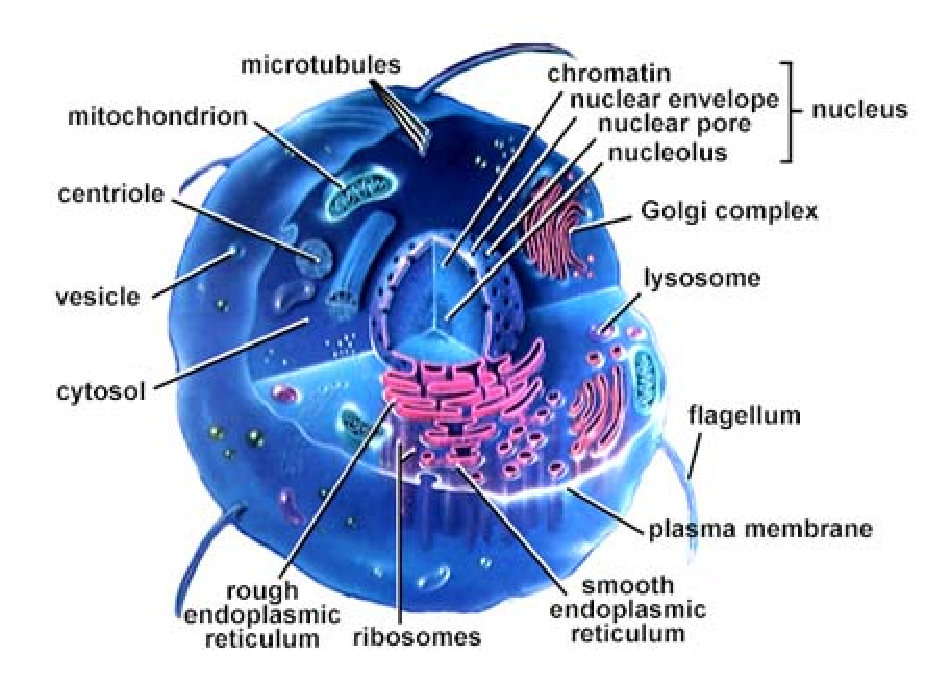
\includegraphics{introduction/eukaryote_cell.eps}}
 \vspace{0.1in}
 \caption{\label{fig:cell}Eukaryote cell}
 \end{center}
 }
 \hfill
 \parbox[b]{0.5 \textwidth}{
 \begin{center}
 \scalebox{0.6}{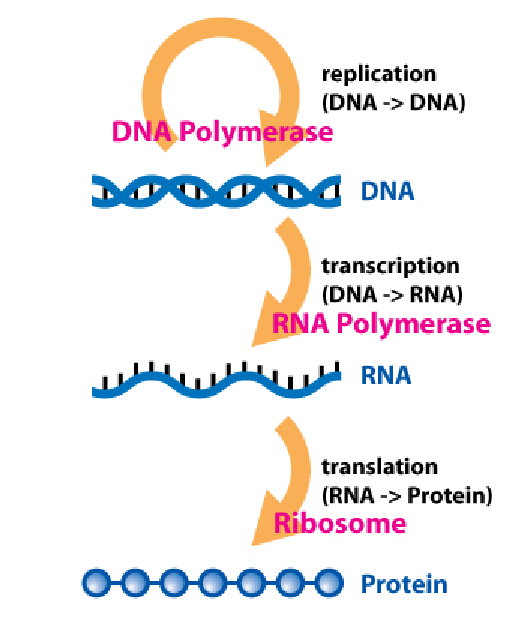
\includegraphics{introduction/central_dogma.eps}}
 \vspace{0.1in}
 \caption{\label{fig:central_dogma}Central dogma of molecular biology: $DNA \longrightarrow RNA \longrightarrow Protein $}
 \end{center}
 }
 \end{figure}

Cells, which are the most fundamental units of life, differ in higher organisms, e.g. multicellular animals and plants, known as \textit{eukaryotes} from those of the less evolved \textit{prokaryotes}, e.g. bacteria, in having a well-defined \textit{nucleus} (see Figure-\ref{fig:cell}\footnote{image taken from online book at \url{http://www.estrellamountain.edu/faculty/farabee/biobk/biobooktoc.html}}) which carries the genetic material. The nucleus is the most prominent structure inside the eukaryotic cell and the genetic information inside it is contained in the form of a \ac{DNA} molecule. \ac{DNA} has a \textit{double-helix} structure formed by two complementary strands, each made up of a sequence of \textit{nucleotides} which are composed of adenine, thymine, cytosine or guanine. 

The central dogma of molecular biology is that the sequence information on the DNA is converted into \ac{RNA} through the process of \textit{transcription}. This sometimes is also referred as \textit{gene expression}. \ac{RNA}, through the process of \textit{translation} is later converted into a sequence of amino acids that results in a \textit{protein} (see Figure-\ref{fig:central_dogma}\footnote{image source: \url{http://en.wikipedia.org/wiki/File:Central\_Dogma\_of\_Molecular\_Biochemistry\_with\_Enzymes.jpg}}). The functional unit on the DNA that codes for an individual protein is known as a \textit{gene}. The sequence of the nucleotides in the double helix within a gene specifies the primary structure of a protein. The complete sequence of nucleotides on the DNA is also referred to as the \textit{DNA sequence}. 
Higher organisms are made up of various different cell types each of which performs a specific role requiring a specific set of gene products. The fascinating fact is that each of these cells contains exactly the same set of genes (DNA) but a different set of gene products. The remarkable diversity among the cells is a result of a precisely controlled mechanism of expression and regulation of a subset of genes in each cell type. 

\begin{figure}[ht]
 \centering
 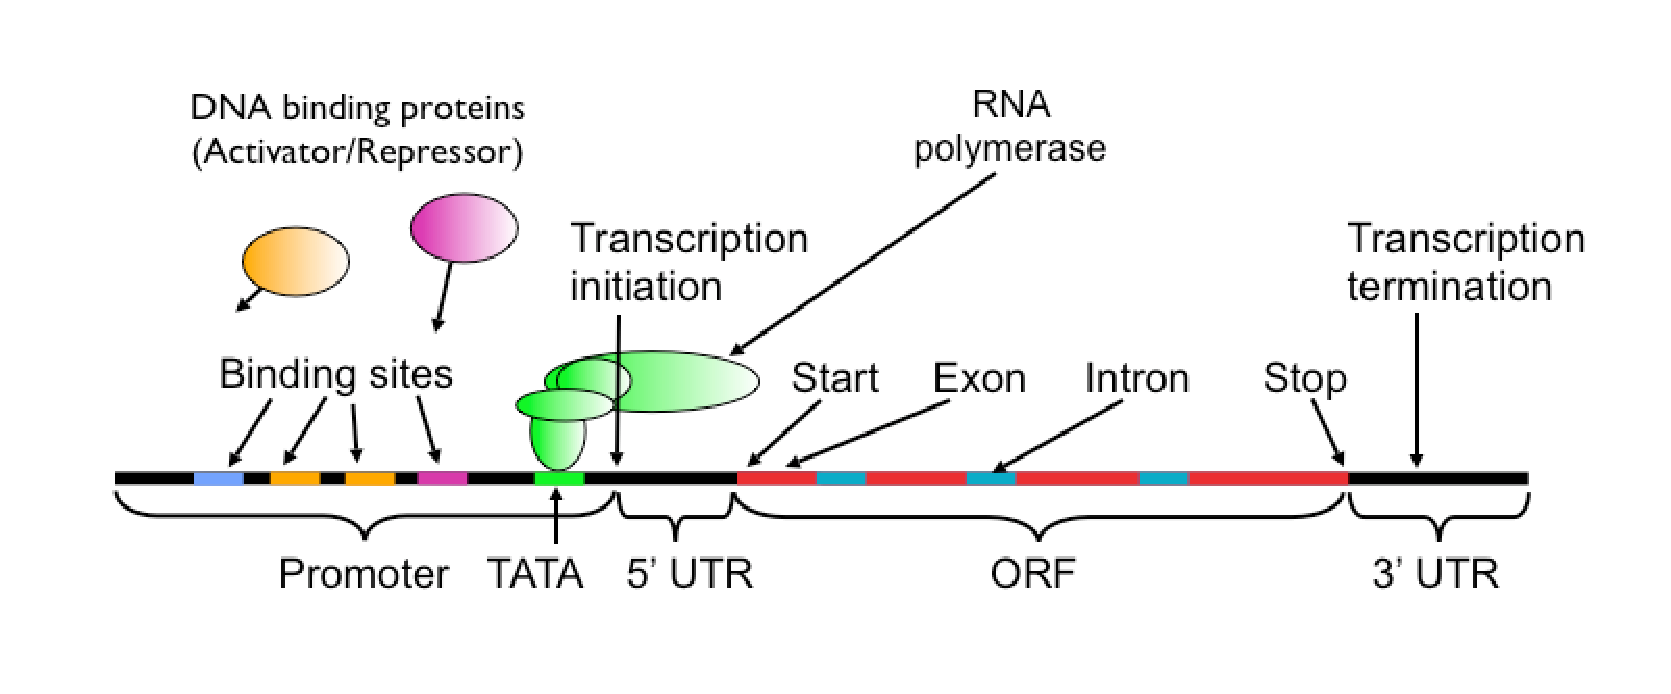
\includegraphics[scale=0.6]{introduction/gene_regulation.eps}
 \caption{Gene regulation}
 \label{fig:gene_regulation}
\end{figure}
The transcription process begins when \acp{TF} are activated by a trans-membrane receptor, leading them to bind to gene regulatory elements and to promote access to the DNA and facilitate the recruitment of RNA polymerase to the transcriptional start site as shown in Figure-\ref{fig:gene_regulation}. The gene regulatory elements of the DNA, also known as \textit{promoter regions}, are situated upstream of the gene at a distance which can vary from a few base pairs to hundreds of base pairs. The regulatory elements contain binding sites for multiple transcription factors allowing each gene to respond to multiple signalling pathways and facilitate fine-tuning of the \acp{mRNA} that are produced. Once the transcription factors are bound on the regulatory elements, they can either promote or inhibit gene expression. In the case of a promoter, the process of transcription starts. A protein called RNA polymerase starts to copy the information contained in the gene into \ac{mRNA}. These \ac{mRNA} molecules, being exact replicas of the gene, contain both \textit{exons} (which will be used in the later process) and \textit{introns} (which will be removed). A process known as \textit{splicing} removes the introns and the remaining \ac{mRNA}, called spliced \ac{mRNA}, is transported out of the nucleus into the cellular material. There it is translated into a polypeptide chain with the help of ribosomes and this chain then folds into a three-dimensional structure known as protein. 

The previous paragraph gives only a partial picture. Since transcription factors themselves are proteins, the same process may regulate them. In fact, there are genes that code just for transcription factors. This process is similar to a feedback loop in which transcription factors are regulated by other transcription factors. A major goal of bioinformatics is to understand how transcription factors affect gene expression and which groups of genes are co-regulated by certain sets of transcription factors. 

\section{Data Sources}\label{bkg:datasources}
Recent technological advances have led to an explosion in both the quantity and types of data being generated. Various observation techniques capture different facets of the cell regulatory process. These are primarily generated by molecular biologists using experimental techniques. Some of the types currently available are:
\begin{itemize}
  \item \ac{mRNA} expression measured using microarrays. 
  \item Whole genome transcription factor binding measured using \ac{ChIP} on chip. 
  \item \ac{TF} binding motifs from the promoter sequences of genes. 
  \item Protein-protein interactions using co-immunoprecipitation and other techniques. 
\end{itemize}

\subsection{Microarrays}
\begin{floatingfigure}[p]{0.45\textwidth}
%\centering
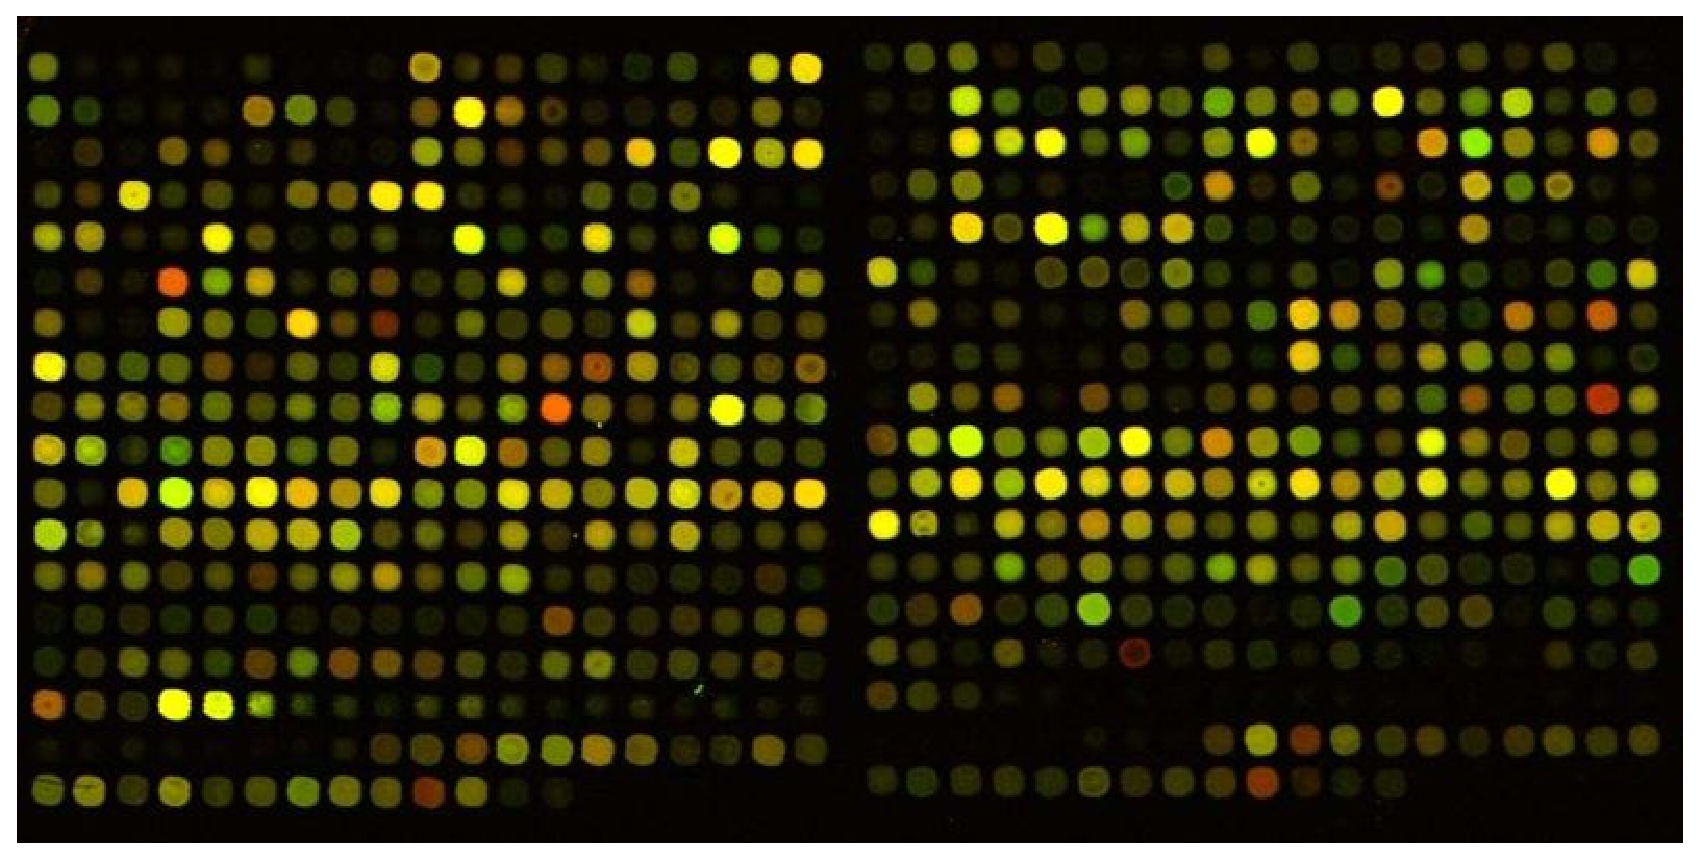
\includegraphics[scale=0.25]{introduction/cdnMicroarray.eps}
\caption{A cross-section of hybridized cDNA microarray}
\label{fig:microarray}
\end{floatingfigure}

One of the most important sources of data related to the transcription process is the genome-wide measurement of \ac{mRNA} expression levels carried out using microarrays. These have received considerable attention in the last six years and various technologies for microarray measurement have been developed \citep{Schulze01navigating}. A microarray allows simultaneous measurement of the expression levels of a large number of genes. It consists of a grid of a large number of microscopic \textit{spots} of DNA oligonucleotides on a silicon chip, each containing a specific DNA sequence. Depending on the specific technique of manufacturing, these are either called \textit{cDNA microarrays} or \textit{oligonucleotide microarrays}. Microarray technology is based on the concept of \textit{hybridization} which means that DNA has complementary strands and given the right conditions, complementary strands will bind to each other. We want to measure \ac{mRNA} content, and since \ac{mRNA} is complementary to the DNA strand from which it was created, it will bind to its complement on the probe. Therefore, each of the spots contain a short section of a gene or other DNA element that we want to study as a probe to \textit{hybridize} a complementary cDNA sample (\ac{mRNA}). Before hybridization, the target is tagged with a fluorescent dye so that after hybridization, the intensity of colour detected by a fluorescence-based detector indicates the abundance of the target.

\textit{Two-channel microarrays} as shown in Figure-\ref{fig:microarray} are hybridized with samples from two conditions, e.g. diseased tissue versus healthy tissue, and are tagged with two different colours. Fluorescent dyes Cy3 (green) and Cy5 (red) are commonly used for tagging these samples. The two coloured cDNA samples are mixed and hybridized to a single microarray that is then scanned. Relative intensities of each colour are then used to identify up-regulated and down-regulated genes. On the other hand, in \textit{single-channel microarrays}, the arrays are designed to give estimates of the absolute levels of gene expression. Therefore, comparison of two conditions requires two separate single-dye hybridizations. 

Similar expression profiles identify genes that may be controlled by a shared regulatory mechanism. Paul Spellman is one of the microarray pioneers who used it to study global expression of genes at various time points in yeast cell cycle \citep{spellman98comprehensive}. He along with some other researchers \citep{gasch00genomicexpn} also studied the response of the yeast genes when subjected to various kinds of stress. Processing microarray data to reduce the errors introduced at various stages is known as \textit{normalization}. \citet{Quackenbush06computational} provides a good overview of the techniques used for normalization and analyzing while \citet{Smythe03Statistical} discuss in detail the statistical issues involved in normalization. 

\subsection{ChIP on chip}

\ac{ChIP} on chip,  also referred to as \textit{ChIP-chip} assay is a technique which allows us to study genome wide binding of transcription factors to the DNA simultaneously. It combines \textit{\ac{ChIP}} with microarray technology (chip) to determine \textit{in vivo} all the regions of interest on the DNA's promoter regions, i.e., where each of the transcription factors bind. \cite{harbison04transcriptional} determined the global genomic occupancy of 203 transcription factors in yeast, which are all known to bind to DNA in the yeast genome. \cite{lee02transcriptional} produced a similar yeast dataset for a smaller number of transcription factors. Both these researchers reported results in the form of a confidence value (statistical P value) of a transcription factor attaching to the promoter region of a gene. The reason behind using statistical techniques was to average the errors in microarray technology and account for multiple cell populations. One of the prominent problems with such approaches is that in order to infer whether a transcription factor attached to the promoter sequence or not, we have to choose an arbitrary artificial threshold of the P-value. 

\subsection{Transcription factor binding motifs}
Transcription factor binding motifs are sequence patterns observed in the intergenic regions of the genome usually located upstream of the genes (promoter region). They are thought to be responsible for allowing access of transcription factors to binding sites which eventually leads to regulation of transcription. While \textit{ChIP-chip} provides \textit{in vivo} evidence of \ac{TF} binding, this is an indirect technique that was used before the advent of \textit{ChIP-chip}. The primary reason for considering this as an information source in the presence of \textit{ChIP-chip} data is that \textit{ChIP-chip} is very noisy and uses evidence from multiple experiments \citep{lee02transcriptional} to report the possibility of a \ac{TF} binding to the promoter region of a gene in the form of a p-value. 

Most of the approaches to identifying these were based on first clustering genes by co-expression, and then looking for common sequences in the upstream regions of the genes located in the same cluster. The upstream sequences are catalogued in the \ac{YPD}, as well as \ac{SCPD} which is dedicated to the curation of yeast genes' promoter sequences \citep{zhu1999scpd}. 

\subsection{Protein-protein interactions}
\begin{floatingfigure}[p]{0.5\textwidth}
%\centering
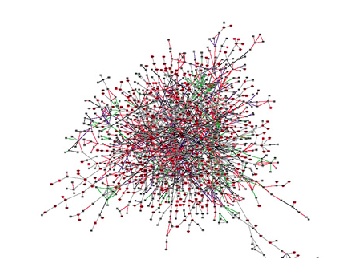
\includegraphics[scale=1.25]{introduction/ppi.eps}
\caption{Protein-protein interactions in yeast}
\label{fig:ppi_yeast}
\end{floatingfigure}
The interactions between proteins is important for many biological functions, e.g. signal transduction, where signals from outside a cell are transmitted to the inside by protein-protein interactions of the signaling molecules. This dataset is important for our study because proteins are gene products and proteins with similar functions and localization are more likely to interact in groups. This was shown by \citet{schwikowski2000protein} where they observed that proteins of known function and cellular location tend to cluster together with 63\% of the interactions between proteins with a common functional assignment and 76\% occurring between proteins found in the same subcellular compartment. Therefore, genes producing interacting proteins are more likely to be co-regulated and have similar functionality. This was verified by \citet{ge01correlation} who provide global evidence that genes with similar expression profiles are more likely to encode interacting proteins. Protein-protein interaction data for yeast is available as a result of advances in technologies like co-immunoprecipitation, mass-spectroscopy and yeast two-hybrid assays. There has been a tremendous growth in this type of data in the recent years. \citet{Gueldener2006MPact} have manually compiled a \ac{PPI} dataset from the literature and published large-scale experiments for yeast which is used as a reference and has been called a gold standard because of its quality and comprehensiveness \citep{yu2004annotation}.
 

\section{Research Goals and Our Approach}
The underlying problem that is addressed results from the nature of the available data. The problem is two fold: firstly, each of the current datasets, e.g. microarrays, DNA-binding, protein-protein interaction and sequence datasets, provide a \textit{partial} and \textit{noisy} picture of the whole process. Hence, we need to integrate them in order to obtain an improved and reliable picture of underlying process. Secondly, the amount of data that is available for each of these types is severely limited. To \textit{learn} good models we need lots of data. Yet, data is only available for few of the experiments of one type. To alleviate this problem many researchers have taken the path of merging available datasets and then learning clusters from it. So, we see that there are two \textit{distinct} types of integration happening, one among \textit{different types} of datasets and the other among datasets of the \textit{same type} but from \textit{different experiments}.

Results are very hard to replicate when the datasets are different even if they result from experiments with the same conditions but done by different experimenters. As clearly stated by \citet{orph02thehuman} there is no single model of regulation and each cell process has evolved its own detailed regulation model. There are certain motifs that can be seen in most of the processes but the actual details of the process are very different from one another. Furthermore, for each underlying motif, the real size of the motif is very different from process to process and geneset to geneset. So, even though many researchers have used this approach of integrating data-sets (both types), its not very clear what the implications on the final results are.

The first part of our research work focuses on \textit{understanding the impact of integration} of the latter type (using datasets of the same type but different experiments) on the global modelling related to the transcriptional gene regulation processes. Most of the algorithms have justified their results \textit{qualitatively} by interpreting their results with the help of biologists. We are interested in studying the \textit{quantitative information overlap} among various datasets and whether our current algorithms are able to leverage the integration of diverse datasets in meaningful \textit{biologically relevant} results. Specifically, we studied the correlation between the theoretical distribution difference among the datasets being merged (using \ac{KL} divergence among distributions) to the functional difference among them (computed using cluster similarity). We also studied how much the functional similarity (in our case, the cluster similarity) varied because of dataset integration as we slowly integrate increasingly diverse datasets. 

The second part of our research deals with proposing a framework and analysis of integrating datasets of different types, e.g. microarray, \textit{ChIP-chip} and PPI datasets. The exact amount of overlap and correlation among functional datasets is unclear \citep{werner2002comparative,kemmeren2002protein}, yet data integration has been shown to increase the accuracy of tasks like gene function prediction compared to single source of data \citep{ge01correlation,gerstein2002proteomics}. For data integration, spectral clustering has been used as our primary tool. The main reason behind this choice is that it is based on computing similarities of variables which results in \textit{affinity} matrices. Similarity computation allows us to normalize diverse datatypes (which were previously considered unintegrable) into a common format (affinity matrices) and then integrate them. Increasingly, biological datasets are non-vectorial, e.g. sequence and PPI data (which is available as a graph). There have been a lot of recent developments in various techniques of similarity computation among these non-vectorial datasets. With this as our foundation, two innovative techniques of integrating these datasets have been proposed.

\subsection{Thesis Scope}
Bioinformatics has grown into a vast field. It is not possible to describe in detail all of the techniques that have been followed or that have been used by the providers of publicly available data. We have not included the details of \textit{within array} normalization techniques of microarray data used by their experimenters and assume that all the microarray data is suitably normalized. 

Even though we have used k-means clustering algorithm, we have not discussed it as it is one of the most well known and elementary techniques. Similarly, we have not discussed the Gene Ontology in great detail. For all these, suitable references have been provided in the thesis.
\section{Thesis Contributions and Publications}
\begin{itemize}
    \item A comprehensive and critical review of research work done in this field has been published as
	\begin{itemize}
	\item Mishra, A. and Gillies, D. (2008). Data integration for regulatory gene module discovery. In Daskalaki, A., editor, \textit{Handbook of Research on Systems Biology Applications in Medicine}. IGI Global, Hershey, PA.
        \end{itemize}	
    \item Issues related to calculation of biological significance of clusters using Gene Ontology has been published as
       \begin{itemize} 
       \item Mishra, A. and Gillies, D. (to be published in 2010). Validation Issues in Regulatory Module Discovery. In: Huma Lodhi and Stephen Muggleton (eds.), Elements of Computational Systems Biology, John Wiley \& Sons, Inc. ISBN: 0470180935.
       \end{itemize}
    \item An empirical technique to calculate the functional similarity of datasets using the concept of cluster similarity has been developed. We propose this can be used as an index for dataset similarity after showing a very high correlation with underlying data distribution differences. We have also demonstrated that dataset integration should only be done by first choosing similar datasets, otherwise the signals present in the datasets could be overwhelmed by noise. Part of this work published as
	\begin{itemize}
	    \item Mishra, A. and Gillies, D. (2007). Effect of microarray data heterogeneity on regulatory gene module discovery. \textit{BMC Systems Biology}, 1(Suppl 1):S2
	\end{itemize}
    \item A semi-supervised spectral clustering technique to integrate two datasets where one is acting as a source of supervision on the clustering of the other has been developed. We validated the results using Gene Ontology.\nocite{mishra2007data,mishra2008Semisup,mishra2007elements} Part of this work published as
	\begin{itemize}
    		\item Mishra, A. and Gillies, D. (2008). Semi supervised spectral clustering for regulatory module discovery. In \textit{Data Integration in the Life Sciences}, pages 192-203.
 	\end{itemize}
    \item A principled technique to integrate two diverse datasets where no evidence is available regarding their individual weights (importance) has been developed using the principle of maximum entropy. We validated the results after spectral clustering of the integrated matrix using Gene Ontology.
    \item Modular and reusable software implementations of all the techniques has been developed using python\footnote{a popular programming language with efficient Linear Algebra library} and R\footnote{a software environment for statistical computing}.	
\end{itemize}

\section{Thesis Outline}
The outline of this thesis is as follows. In Chapter-2, we present a critical literature review related to the evolution of the research related to transcriptional regulatory networks and modules. Even though this field is relatively new, the amount of research done is enormous because of increasing focus and funding. This chapter tries to tie together all the past efforts into a coherent story. 

In Chapter-3, we study the effect of \textit{integrating increasingly diverse microarray datasets}. For functional similarity, we compute the cluster similarity among datasets using modified Rand's index. To estimate the theoretical difference between the underlying distributions of individual datasets, we use the \ac{KL} divergence. Finally, we study the correlation between the two measures (functional and theoretical).

In Chapter-4, we start with a discussion of spectral clustering and its theoretical foundations. In order to integrate microarray datasets with other datasets e.g., PPI and DNA-binding datasets, we propose a semi-supervised spectral clustering technique. We apply this technique on two of the popular yeast microarray datasets and evaluate the results of integration using the Gene Ontology. 

While the semi-supervised algorithm is heuristic in combining separate evidence of similarity, in Chapter-5, we propose a more principled approach to integration of similarity matrices. We merge similarity matrices derived from various datasets (microarray, PPI and DNA-binding) using the principle of maximum entropy \citep{jaynes57maxent} and analyze the results.

Finally, Chapter-6 concludes this thesis with remarks about the drawbacks and challenges faced in our approach. It details where the field is heading and what would be the future challenges. We also discuss the scope and direction of extending the current work in future. 


\chapter{Regulatory Module Discovery Algorithms}
In this chapter, we review the research done in data integration techniques for regulatory module discovery. Initial research in this area involved plain clustering of microarray data. This was followed by progressively sophisticated modelling as well as integration of various data types.
   
\section{Plain Clustering} 

When microarray data started becoming available in the late 1990s, a prime goal was to identify sets of genes that act together functionally to perform certain cellular tasks such as metabolism or cell-cycle functions. In this early phase of data analysis, various clustering algorithms, e.g. \citet{eisen1998cluster}, were applied in order to find such gene modules.  An assumption behind this clustering approach was that co-expression implied co-regulation. In other words, if sets of genes were showing similar patterns of microarray expression, they must be co-regulated and hence belong to the same module. So, co-expression was assumed to imply co-regulation and co-regulation was assumed to imply similar function. However, both these assumptions are not always correct. The validity of the resulting clusters could be tested by identifying common promoter elements on the upstream portion of genes within the same cluster on the assumption that genes are co-regulated because they have similar promoter elements. Another popular way to show validity was by using gene ontology to show that the majority of genes belonging to a module were similar in function. This was done by computing the enrichment of gene ontology terms in each of the clusters. Better clusters were expected to have more significant enrichment of these terms. In these early works, no external information was used to guide the process of clustering. A review of the early techniques based on ad-hoc as well as model based clustering can be found in \citet{jong02modeling}.

\section{Causal Networks} 
Naturally, the research community wanted to model the causal relationships among various genes in much more detail, and this precipitated a second phase of modelling in which mostly Bayesian networks and their variants, such as dynamic Bayesian networks (DBNs), were applied to model the gene regulatory processes \citep{friedman00using,husmeier03sensitivity,murphy99modelling,zou05dynamic}. \citet{friedman00using} were the first to utilise Bayesian networks for modelling gene expression data and they tried two types of local distribution - discrete (multinomial) and continuous (linear Gaussian) to express the relation between dependent genes. They tested the work on the microarray expression data of \citet{spellman98comprehensive}. When networks that modelled the data accurately were identified, two pairwise features were computed from them - Markov relations and order relations. The Markov relation just checks if each gene of a pair is in the Markov blanket of the other. This would imply a direct causal relationship between them indicating a biological relation. The order relation checks if X is ancestor of Y in all the networks of an equivalence class. This can be determined directly from the directed graph by checking whether there is a path from X to Y that is directed towards Y consistently. An order relation implies that the two genes have a role in some more complex regulatory process. Temporal aspects of data were incorporated into the model by adding a discrete variable as the root. They suggested that non-linear local and temporal models should be used for better accuracy. Their analysis of the results shows that the method is sensitive to the choice of local model and in the case of the multinomial distribution is also sensitive to the discretization method used. \citet{werhli06comparative} carried out a comparative study of the performance of modelling gene regulatory networks using \acp{GGM}, relevance networks and \acp{BN}. They used both laboratory data as well as simulated data to evaluate the different approaches. They observed that on both types of data, Bayesian networks outperformed both relevance networks and graphical Gaussian models. 

The major difficulty with this fine tuned modelling approach is that for such a high dimensional problem involving many thousands of genes, the amount of experimental data available is never enough for accurate modelling. Moreover, it is very hard to deal with the cyclical feedback nature of gene networks using Bayesian networks since, without the explicit incorporation of time, they only handle acyclic relationships among the variables. The end result of such models was that the performance was not good and not many verifiable findings were made \citep{husmeier03sensitivity}. In order to improve upon the results, work was done to incorporate better prior knowledge in the Bayesian network based modelling. \citet{imoto03combining} combined PPI, DNA binding, promoter element motifs as well as literature text mining. \citet{tamada03estimating,tamada05utilizing} also used similar diverse datasets to build Bayesian network models. 

\citet{ihmels02revealing} proposed an algorithm called \textit{Signature}, which performs bi-clustering, that is to say clustering genes, and conditions together based on expression data. It is unlike the more established bi-clustering algorithms in that it does not simultaneously generate data partitions but works in steps. The input to the algorithm is a set of genes and, in the first step, experimental conditions under which these genes change their expression above a threshold are chosen. In the second stage, all genes that have changed expression significantly under these conditions are selected. They evaluate the consistency of their clustering algorithm by analysing the recurrence of the output gene sets in their resulting modules when the input is mixed with irrelevant genes. The idea is that the results of any good algorithm should not deviate too much when slight perturbations are introduced in the data. A module is considered to be reliable if it is obtained from several distinct slightly perturbed input gene sets. Since it carries out a refinement of clusters in two stages, there can be no guarantee that the results would be clustered in a globally optimal manner. A better formulation might be to use the \ac{EM} algorithm in order to maximise their objective function. 
 

\section{Supervised Module Algorithms} 

After these initial frustrations in moving from very naive modelling (plain clustering) to highly detailed modelling (\acs{DBN}), research began to tread a path somewhere in the middle. This pragmatic approach did yield very good results and is still the basis of current research. One of the most complete studies using these types of weakly supervised methods was carried out by \citet{segal03module}. Their method, called \textit{Module Networks} algorithm, takes as input a gene expression data set and a large precompiled set of candidate regulatory genes and outputs groups of co-regulated genes (modules), their regulators, and a regulation program that specifies behaviours of the modules as a function of regulator's expression and the conditions under which regulation takes place. It uses an iterative procedure that searches for a regulation program for each module (set of genes) and is based on the \ac{EM} method that is initialised with the results of another clustering algorithm. For each cluster of genes, it searches for a regulation program that provides the best prediction of the expression profiles of genes in the module as a function of the expression of a small number of genes from the regulator set. After identifying regulation programs for all clusters, the algorithm re-assigns each gene to the cluster whose program best predicts its behaviour. It iterates till convergence, refining both the regulation program and the gene partition in each iteration. 

In their experiments, they compiled a set of regulators from the \ac{SGD} \citep{cherry98sgd} and the \ac{YPD} \citep{payne98ypd} based on annotations that broadly suggest that certain genes have a regulatory role, as either a transcription factor or a signalling protein. They also identified more potential regulators by finding genes similar to those above but removing the global regulators from the list. Microarray data for gene expression for yeast was collected from the \ac{SMD}. They chose a subset that had significant gene expression change and removed from this set the cluster known to be generic environmental response genes. Finally, they added all the genes from the regulator list above. With these two datasets (expression and regulators), they use a module network learning algorithm \citep{segal05learning} to find separate sets of regulators and the regulated modules. They obtained modules that showed significant similarity in promoter element motifs as well as annotations in the gene ontology compiled by the Gene Ontology \citet{GO}. 

At about this time, more significant prior knowledge started becoming available in the form of ChIP-chip DNA binding data and other sources as described in the previous chapter. The next step of research focused on ways of integrating these datasets in order to find gene modules. 

\citet{barjoseph03computational} describe an algorithm for discovering regulatory modules. Their algorithm is called \ac{GRAM}, and combines microarray expression data with DNA-binding data. This was one of the first papers to have combined these two sources in order to achieve better clusters. DNA-binding data provides direct physical evidence of regulation and thus offers an improvement on previous work where only indirect evidence of interaction, for example promoter sequences, were used for prior information. The GRAM algorithm begins by performing an exhaustive search over all possible combinations of transcription factors indicated by the DNA-binding dataset using certain (strict) threshold P-values. This yields sets of genes that are regulated by sets of transcription factors. This gene list is filtered by studying their expression patterns to find genes that show co-expression. These act as seeds for gene modules. The next pass revisits transcription factors and expands the seed modules by adding genes with a relaxed P-value criterion that show co-expression. GRAM allows a gene to be part of more than one module. They identified 106 modules with 655 distinct genes regulated by 68 transcription factors. Within a module, the role of each transcription factor was identified as activator or repressor by analysing the correlation between the transcription factor's expression and the expression of regulated genes. Validation was done by analysing the promoter gene sequences in same cluster using the TRANSFAC \citep{transfac1996} database to identify common sequences. 

\citet{AmosTanay04revealing} analysed several diverse datasets in an attempt to reveal the modular organisation of the yeast regulation system. They defined modules as groups of genes with statistically significant correlated behaviour across the diverse datasets. Their algorithm is called \ac{SAMBA} which is an extensible framework that can be easily updated when new datasets become available. In their analysis, they have integrated expression, PPI and DNA-binding datasets. In \ac{SAMBA}, all genomic information is modelled as weighted bi-partite graphs. Nodes on one side of graph represent genes while the other side represents properties of genes, for example proteins encoded by them. Edges between property nodes and gene nodes are assigned weights. A module is a sub graph of this bi-partite graph and a high quality module is defined as a heavy sub graph in the weighted bi-partite graph. The key point is that all sources of data are considered as properties of genes or proteins encoded by genes and there is one unified representation of all data as a bi-partite graph. Since their algorithm is based on combinatorial principles rather than graph theoretic (spectral) methods, there are no guarantees of a globally optimum partitioning. For evaluation, they found the biological significance of resulting clusters by calculating the enrichment score of all gene ontology (GO) terms associated with the genes of a module and later annotated the modules with the highest valued terms, that is to say those terms that are shared by the highest number of genes. They also analysed 600 base pairs in the upstream promoter region of the genes in a module for common motif enrichment. For each potential motif, they calculated the enrichment score among all the genes of the module. The positive aspect of their approach is that it utilises all sources of information in one uniform representation and only requires a measure of similarity of genes across a subset of properties. It also allows overlapping modules (with common genes), which is not a feature of traditional clustering algorithms. One of the limitations of their approach is that all sources of data are assigned equal weights and it isn't possible to weigh them separately according to reliability or importance. 

In a later piece of work, \citet{amos05integrative} extended the work described above by investigating the \ac{SAMBA} algorithm in more detail. They analysed more diverse datasets and focused more on the biological significance of the results, explaining them much more fully. The paper mainly describes a study of fresh data in the context of an extensive compendium of existing datasets using \ac{SAMBA}. They proposed that future work should be carried out on integration across species on the basis that transcription modules are highly conserved among species. 

The work of \citet{lemmens06Inferring} is similar to other module discovery algorithms in that they propose a very simple and intuitive algorithm to find co-regulated sets of genes that have similar expression profiles, the same binding transcription factors and a commonality of promoter motifs. The principal difference from other algorithms is that where others used motif information to validate their results, they have used it in order to find the modules itself. Their algorithm, known as ReMoDiscovery works in two passes. In the first pass, known as the \textit{seed discovery} step, tightly co-expressed genes having a minimum number of common transcription factors and a minimum number of common conserved motifs are put together in separate modules known as \textit{seed modules}. In the second pass, known as the \textit{seed extension} step, the size of the modules is increased by computing the mean of the module's gene expression and ranking the remainder of the genes in the dataset in order of their decreasing correlation with the mean profile. They compared their algorithm results with \ac{SAMBA} and \ac{GRAM} (discussed earlier) and reported their findings. All parameters, such as the cut off for various datasets, have been chosen without much justification, and the basic idea seems very similar to the work of \citet{barjoseph03computational}. Some of the comparison metrics used do not seem very sound, for example average functional enrichment values have been calculated for the modules without normalising to account for the size of the modules. Similarly, summary statistics like minimum and maximum number of genes in modules do not provide relevant information for comparison of algorithms . 

\citet{huang2006incorporating} investigated a traditional clustering method known as k-medoids which is a robust version of the k-means clustering method. Unlike k-means, which uses the mean of all genes in a cluster as its centre, k-medoids uses the most central gene (median). It is found by locating the one with minimum average dissimilarity to rest of the genes. They incorporated prior knowledge into it by modifying the distance metric used while clustering. They have used microarray expression data for clustering while biological knowledge about the known similarity between pairs of genes is derived from gene ontology. Previous approaches to include biological knowledge in distance based clustering methods have used gene ontology and metabolic pathways to estimate distance or similarity measures among gene pairs and then used these along with microarray expression based distance metrics to create an average distance, which is later used to cluster expression data. Huang and Pan used a \textit{shrinkage} approach for the distance metric to shrink it towards zero in cases where there is strong evidence that two genes are functionally related. Their algorithm has two steps in which the first step uses the shrunk distance metric to cluster genes whose functionality is known from gene ontology. The second step clusters the remaining genes. In the second step clustered genes are assigned to either one of the step one clusters or to a step two cluster, depending on their distance from the medoids. The shrinkage parameter is chosen using cross validation. They evaluated their algorithm using both simulated as well as real data. In a later piece of work, \citet{pan06incorporating} used known functions of genes from existing biological research to assign different prior probabilities for a gene to belong to a cluster. He developed an \ac{EM} algorithm for this stratified mixture model. 

The research described above concerns the evaluation of individual techniques to integrate data from multiple sources. Some researchers have also focused on creating generic frameworks for data integration. \citet{Troyanskaya2003Bayesian} developed a \textit{meta} framework for integration of diverse sources of data. We call it \textit{meta} because it doesn't directly integrate the datasets but uses results from other techniques like clustering algorithms and combines them with other evidence. Their proposed framework is known as MAGIC (Multisource Association of Genes by Integration of Clusters) and is based on a Bayesian network whose conditional probability tables have been built with the advice of yeast genetic experts. Given a pair of genes, it outputs the probability that they are functionally related after weighing the evidences from various sources. Evaluation of the predictions from the system is done using gene ontology data. 

Most of the techniques that we have described work well for real (numerical) data but are less effective when dealing with string data, for example gene sequences, or graph data such as protein interactions. In many cases ad-hoc techniques have been deployed. In an approach to this problem, \citet{lanck04statframework} have proposed a framework where such diverse data could be merged in a principled manner. It is based on kernel methods \citep{johnshaw2004kernelmethods} in which algorithms work on kernel matrices that are derived from pairwise similarity among variables using kernel functions. If a valid kernel function can be defined to encode the similarity between two variables, then the methods are applicable regardless of the different types of data - strings, vectorial or graphical - being used. This framework provides a means to integrate more diverse types of data as and when they become available in the future. The original paper proposed the framework only for supervised learning but extensions to unsupervised learning are possible. 



\chapter{Data Integration for Regulatory Module Discovery}
\section{Introduction}

As discussed in the first chapter, a transcriptional regulatory module is a set of genes that is regulated by a common set of \acp{TF}. A considerable amount of work has been carried out to determine the network of inter-relationships between these regulatory modules, with the aim of understanding how they act together in order to carry out the complex biological functions of a cell. Microarrays allow us to study a large proportion of genome expression simultaneously. These expression data have been used to build models of the regulatory networks. In some of the recent work, \textit{integrative genomics}, in which data from experiments relating to different conditions or even different organisms are merged together, has been suggested as a method to discover these regulatory modules \citep{amos05integrative,segal04module}. The approach compensates for the fact that the models have a very large number of variables (genes) whereas the number of repeats of microarray experiments is typically quite small. Thus, for a typical single experiment, there is not enough data to model the regulatory modules reliably. Another justification for the integrative approach is that, in evolution, many genes are believed to have similar roles in different organisms and so collective analysis should help to counter experimental error in individual experiments.  

The motivation behind the research presented in this chapter is that, in our view, \textit{blind} integrative genomics can lead to misleading or incorrect results. Researchers conduct experiments with clear objectives in mind. For example, research conducted on yeast to study meiosis will profile gene expression in sporulation media and will have clear meiotic signal in the data. But, hardly any of these conditions will be in common with the experiments related to stress conditions on yeast. Integration should be used when we are \textit{only} concerned about either the background patterns or the most dominant patterns, and are not interested in patterns that may be visible in certain individual experiments. The global regulatory module network is the sum of smaller local regulatory module networks and by taking the integrative approach we run the risk that significant information from individual networks will be masked by the pooling process.

We believe that integrative genomics can sometimes be a useful technique. Our hypothesis is that as microarrays from different experimental conditions but same experiment type, for example stress, are merged, we should be able to readily identify stress specific regulatory modules. The clusters of co-regulated genes obtained should reinforce the local (stress specific) regulatory modules while suppressing the noise. By contrast, when microarrays from various different experiment types are merged together then the local (dataset specific) regulatory modules would be masked by conflicting patterns from other diverse datasets. Only sets of the genes that are strongly expressed among the majority of the conditions for which datasets have been mixed would be observed to behave in a consistent manner while the other genes would be expressed in an unpredictable manner. This should result in regulatory modules that are not very similar to the modules obtained with the original datasets.

One possible way of determining the similarity between datasets is using a statistical measure like the Kullback-Leibler divergence between the distribution of the different datasets \citep{ernstwit2004statis_microarrays}. We computed the difference in data distributions of various distinct and progressively mixed microarray datasets as discussed later. However, the problem with Kullback-Leibler divergence or other statistical methods is that such a theoretical measure is not guaranteed to be a good indicator of \textit{functional} similarity. They don't say much about how the final clusters are affected when we mix datasets. Therefore we validated our results by taking the functional route and studying the eventual effects directly by calculating the similarity among the resulting modules. We carried out experiments in which we obtained regulatory modules from various datasets and their mixtures and then measure their similarities to each other. In this way, we show that progressive mixing of data of differing types inhibits the discovery of local regulatory modules at the cost of more dominant regulatory modules. 

For our experiments, we chose to use the Module Networks algorithm \citep{segal03module} (refer Chapter-2), which is a well established approach and has had recognised success in finding biologically relevant modules. For measuring the similarities among the regulatory gene modules resulting from this algorithm, we chose to use the \textit{modified Rand Index} \citep{hubert85comparing} which has been shown to be a very stable measure of partition similarity. To our knowledge, there hasn't been any thorough study investigating the effects of mixing diverse datasets on the resulting clusters. We also haven't seen any research on understanding the correlation between theoretical data distributions and its impact on the resulting clusters.

\section{Methodology}\label{method}
In order to validate our hypothesis, we chose to work with two very diverse datasets compiled from yeast experiments. One of them is from experiments to study the gene expression when yeast is exposed to stress conditions. The other dataset was from the study of cell-cycle related genes in which the pattern of activity is very different from the previous one. The expression of genes when stress conditions are created is much more drastic (both repressed and induced genes) than the normal cell-cycle, where optimal conditions are created for growth and the expression levels are much smaller. We want to show how progressive dilution of these two datasets with other dissimilar datasets affects the similarity among resulting clusters. We would expect that, as we dilute the datasets, the resulting cluster similarity to the original dataset cluster decreases.

All the data used in our analysis were taken from the \ac{SMD} \citep{sherlock01smd} which hosts c-DNA microarray data-sets from various experimenters. We decided to focus our study on yeast as the regulatory mechanisms in more complex organisms are more involved and yeast has been studied extensively in recent years. We started with analysing data by individual researchers for experiments related to stress. In particular, we used data from \citet{gasch00genomicexpn} submitted by A.P. Gasch which we refer to as DS-STRESS1 (76 microarrays), \citet {saldanha04nutritional} called DS-STRESS2 (49 microarrays) and \citet{gasch00genomicexpn} submitted by P. Spellman called DS-STRESS3 (41 microarrays). We merged all 183 stress related microarray slides available (not only the above three) to create the data set that we refer to as DS-STRESS. To compare these clustering against an entirely different category, we took 93 microarray data sets for cell-cycle experiments \citep{spellman98comprehensive} referred to as DS-CCYCLE. A further mixing of both stress and cell-cycle data created a data set that was named DS-STRESS-CCYCLE (276 microarrays). Finally, we pooled all the available data (523 microarrays) for yeast (not only stress and cell-cycle) and named it DS-ALL. The clusters resulting from all these different data groupings were compared. In order to have a reference point to compare the similarity values, we also generated a random microarray dataset for all the genes by sampling random numbers from a Gaussian distribution with zero mean and unit standard deviation. This dataset was named DS-RANDOM.

To analyze the data we did some standard pre-processing to the datasets. We used the $log_{2}$ of the ratio of the mean of Channel 2 (experimental expression) to the mean of Channel 1 (control expression). We also used total intensity normalization which is based on the assumption that the average log ratio on the array should be zero. Having organised the data, we did three types of studies with the following further processing.

\begin{enumerate}
\item We took all the data described above without further processing.

\item We filtered the genes by choosing those where log(base2) ratio had changed by two fold at least once among all experiments. This retains only those genes that have shown significant change in their expression.

\item We scale normalized each of the above data-sets (without any filtering) across slides to account for different experimental conditions or different data-sets by using a variant of \ac{MAD} \citep{yang02normalization}. Note that this is different from normalizing microarray replicates for removing noise. The data that we are using has already been normalized to account for that. \ac{MAD} is a measure of statistical dispersion and is a more robust estimator of scale than the sample variance or standard deviation. MAD is unaffected by the magnitude of the distances of a small number of outliers whereas in the standard deviation, the distances from the mean are squared, therefore, large deviations are weighted more heavily, and thus outliers can heavily influence it. For our computations, the \ac{MAD} for the $i_{th}$ slide (or condition) is given by
\begin{equation}
MAD_{i}=median_{j}\{\mid M_{ij}-median_{j}(M_{ij}) \mid\}
\end{equation} 
where $j$ ranges across all the genes, $i$ ranges across all the slides (conditions) and $M_{ij}$ is the individual microarray value. We compute the \ac{MAD} value for all the slides and then normalize this score for each slide by taking into account other slides.
\begin{eqnarray}
{a}_{i}&=&\frac{MAD_{i}}{\sqrt[I]{\Pi_{i=1}^{I}MAD_{i}}} \\
M_{ij}(final) &=& \frac{M_{ij}}{a_{i}^{2}} 
\end{eqnarray}

As suggested by the authors, we have divided each value for slide $i$ by $a_{i}^{2}$. This normalization takes into account the \acp{MAD} for all slides and has been found as a reliable way to normalize variation across slides in microarray studies \citep{yang02normalization}.

\end{enumerate}

\subsection{Kullback Leibler divergence among datasets}\label{kl-divergence}
Before we start computing the cluster similarity among datasets, we first need to understand how different (quantitatively) the underlying data distributions are. For this, we have used the \ac{KL} divergence which is a statistical measure to compare distributions. 

For two distributions F and G with densities f and g respectively, the \ac{KL} divergence between them is defined as 
\begin{equation}
d_{KL}(F,G) = \int_{-\infty}^{\infty}f(x)log\frac{f(x)}{g(x)}dx
\end{equation}

However, \ac{KL} divergence is not a distance measure as it lacks symmetry (($d_{KL}(F,G)\neq d_{KL}(G,F)$)), i.e., the \ac{KL} divergence from F to G is not the same as from G to F. There have been some suggestions regarding how to make it symmetric. \citet{Jeffreys46} suggest that it should be modified to 

\begin{equation}
d_{Jeffreys}(F,G) = \frac{d_{KL}(F,G) + d_{KL}(G,F)}{2} \label{KL-Jeffreys}
\end{equation}
which is the mean of both the values. \citet{Johnson01symmetrizing} suggest the harmonic mean and name it as resistor-average mean
\begin{equation}
\frac{1}{d_{Resistor}(F,G)} = \frac{1}{d_{KL}(F,G)} + \frac{1}{d_{KL}(G,F)} 
\end{equation}

We have used the $d_{Jeffreys}$ to validate our results. Determining the underlying distribution of microarray data is another challenge, and more so with so few replicates. We have assumed that the gene expression data across slides (experiments or conditions) has a Gaussian distribution following \citet{ernstwit2004statis_microarrays} who have found that after a logarithmic transformation, most microarray gene expression values across slides have a Gaussian distribution. Another key benefit is that a Gaussian distribution yields an analytically simple and elegant computable form. If $r_{F}$ and $r_{G}$ replicate arrays are spotted for conditions F and G and p is the total number of genes then the two microarray datasets (F and G) could be represented as
\begin{eqnarray*}
f_{ij}: i = 1,\dots p, j = 1,\dots ,r_{F} \\
g_{ij}: i = 1,\dots p, j = 1,\dots ,r_{G}
\end{eqnarray*} 

and the empirical \ac{KL} divergence under the assumption of normality (Gaussian distribution) can be calculated as \citep{ernstwit2004statis_microarrays}

\[
\hat{d}_{KL}(F,G) = \sum_{i=1}^{p} \big[ log \frac{\hat{\sigma}_{gi}}{\hat{\sigma}_{fi}} + \frac{1}{2} \big( \frac{\hat{\sigma}_{fi}^2}{\hat{\sigma}_{gi}^2} + \frac{(\hat{\mu}_{gi}-\hat{\mu}_{fi})^2}{\hat{\sigma}_{gi}^2} -1 \big) \big]
\]
 
where 
\begin{eqnarray}
\hat{\mu}_{fi} &=& \frac{1}{r_{F}}\sum_{j=1}^{r_{F}}f_{ij} \\
\hat{\sigma}_{fi} &=& \frac{1}{r_{F}-1}\sum_{j=1}^{r_{F}}(f_{ij}-\hat{\mu}_{fi})^2
\end{eqnarray}
are the sample mean and variance of the observations associated with the $i_{th}$ gene. It should be noted that this assumes that each of the genes have a univariate Gaussian distribution and they are independent of each other. In essence we are computing pairwise \ac{KL} divergence between corresponding gene replicate data from two different experiments.

\subsection{Cluster similarity}\label{cluster_similarity}
For clustering, we have used the software package Genomica \citep{segal03module} which has been provided by the authors of the Module Network algorithm. The reason we chose this algorithm was because it has been shown in literature to identify biologically meaningful clusters. Its clustering process is driven by the expression of known TFs. The algorithm works as follows: given a gene expression dataset and a precompiled set of candidate regulatory genes, it simultaneously searches for a partition of genes into modules, and for a regulation program for each module that explains the behaviour of the genes in the module. It uses an \ac{EM} approach to do the search. For each module, the procedure searches for a regulation program that provides the best prediction of expression profiles of the genes in the module as a function of the expression of a subset of genes from the candidate regulator set. The approach is iterative and runs till convergence, refining both the regulation program and the gene modules in each iteration. 

This algorithm, apart from microarray data, also requires a list of \acp{TF} as prior knowledge on which to base the clustering. Our TFs were taken from the Yeastract database \citep{Teixeira06yeastract}\footnote{using their web interface \url{http://yeastract.com/} in Sept. 2006 when it had 145 TFs}. 

Since we are comparing the results on different data-sets our goal is to check the closeness of these resulting clusters (on different data-sets). This closeness was validated using \textit{cluster similarity} as described in the next section.

\subsection{Cluster similarity indices}
In order to compare the clusterings obtained on the different datasets, we need a measure of similarity. We have chosen a well established measure of clustering similarity - the \textit{adjusted Rand's Index} - which was proposed by \citet{hubert85comparing}. 

The Rand's index works on the concept of pair-wise matching on each of the cluster sets that are being compared. Given a set of objects of cardinality $n$, $S = {s_1, . . . , s_n}$, suppose we obtain two clusterings $C1$ and $C2$ such that $C1 = {c1_1, . . . , c1_k}$ and $C2 = {c2_1, . . . , c2_k }$ where $\bigcup_{i=1}^{k}c1_{i} = S = \bigcup_{j=1}^{k}c2_{j}$. If:
\begin{eqnarray*}
N_{11} & = & \mbox{number of pairs of objects in the same cluster in both C1 and C2}\nonumber\\
N_{00} & = & \mbox{number of pairs of objects in different clusters in both C1 and C2}\nonumber\\
N_{01} & = & \mbox{number of pairs of objects in different clusters in C1 but same cluster in C2}\nonumber\\
N_{10} & = & \mbox{number of pairs of objects in the same cluster in C1 but different clusters in C2}\nonumber\\
\end{eqnarray*}

then \textit{agreement(A)} is the sum of $N_{11}$ and $N_{00}$ and \textit{disagreement(D)} is the sum of $N_{01}$ and $N_{10}$. \textit{A} is the sum of pairs where both clusterings agree and \textit{D}, where both disagree. The Rand's index is simply the fraction in \textit{agreement} to the total (\textit{agreement} + \textit{disagreement}), i.e.,
\[
R_{C1C2}=\frac{(N_{11} + N_{00})}{(N_{11} + N_{00}+N_{01} + N_{10})}
\]
and its value lies between 0 and 1. When the two partitions are identical, the Rand's index is 1. It falls to 0 when the two clusters have nothing in common. The biggest drawback of this index is that it doesn't have a good spread of values. Another problem with the Rand's index is that the \textit{expected} value of two random partitions does not take a constant value. This is an expected statistical property of any good index to compare clusterings. The modified version of the Rand's index - also known as \textit{adjusted} or \textit{modified Rand's index} corrects for this by assuming the general form
\[
R_{C1C2adj}=\frac{\text{index value - expected(index value)}}{\text{maximum(index value) - expected(index value)}}
\]
For a detailed derivation of the analytical form of this equation, please refer \citet{hubert85comparing}. 
\begin{table}[t]
\centering
\begin{tabular}{|c|c|c|}
\hline
Datasets & \multicolumn{2}{|c|}{Cluster Similarity Index} \\
& Rand's &  \textit{adjusted} Rand's \\
\hline
DS-STRESS3 \& DS-RANDOM & 0.945 & 0.001 \\
DS-STRESS3 \& DS-CCYCLE & 0.946 & 0.100 \\ 
DS-STRESS3 \& DS-STRESS3 (different runs) & 0.957 & 0.453 \\
\hline 
\end{tabular}
\caption{Comparison of Rand's Index and \textit{adjusted} Rand's Index}
\label{tab:rand_vs_adjustedrands}
\end{table}

Its maximum value is 1 and its expected value in the case of random clusters is 0. Based on an extensive empirical comparison of several such measures, \citet{milligan85exam} recommended this index as the best measure of agreement even when comparing partitions having different numbers of clusters. We did a comparison of Rand's and \textit{adjusted} Rand's index on our clustering results. Table-\ref{tab:rand_vs_adjustedrands} shows that the spread of values by Rand's index is skewed (all the values seem to be above 0.94). On the other hand, the \textit{adjusted} Rand's index shows a very wide spread of values. Based on this justification, we chose to use it for all our cluster comparisons. Our whole methodology is summarised in Algorithm-\ref{alg:cluster_comparison}.

\begin{algorithm}
\caption{Summary of methodology}
\label{alg:cluster_comparison}
\begin{algorithmic}[1]

\STATE Pre-process the datasets using the filtering and normalization steps discussed earlier to create 3 separate datasets (normal, filtered and scale normalized).
\STATE Process (mix) datasets so that they contain data from progressively diverse microarray experiments. 
\STATE Run clustering algorithm over each of these resulting datasets. 
\STATE Calculate cluster similarity among the resulting sets of clusters.
\STATE Compute \ac{KL} divergence among all these datasets.
\STATE Compute the correlation coefficient between the cluster similarities and \ac{KL} divergences.
\end{algorithmic}
\end{algorithm}

\section{Results}
\subsection{Cluster similarity among datasets}
\input{chapter1/cluster_similarity}

The results of cluster similarity computations are in Tables-\ref{results:unnorm}, \ref{results:filtered}, and \ref{results:norm}. The clustering algorithm groups together \textit{functionally} similar genes. By using the modified Rand index, we measure the similarity among the resulting sets of clusters. We ran the clustering algorithm 4 times for each dataset and have reported the mean values of all these runs. This was done because the initialization of the clustering algorithm is done by another non-deterministic algorithm. We observed that the final results did not have significant standard deviation (values in brackets in Table-\ref{results:unnorm}\subref{results:unnorm:intra_class_clustering_variation}). For clarity of presentation, we have not reported standard deviation values in remaining tables.

We first compared the individual stress datasets to each other to compare how similar the various runs of the same dataset are as well as to other stress datasets. We then compared each of the stress datasets against DS-STRESS, DS-STRESS-CCYCLE, DS-ALL, DS-CCYCLE which are increasingly distant from the stress datasets as described earlier. As a reference, we also compared them against DS-RANDOM which is a randomly generated dataset and gives us a baseline against which to compare the rest of the similarity values. 

The values in Table-\ref{results:unnorm}\subref{results:unnorm:intra_class_clustering_variation}, \ref{results:filtered}\subref{results:filtered:intra_class_clustering_variation}, and \ref{results:norm}\subref{results:norm:intra_class_clustering_variation} indicate the level of similarity among the same type of datasets. The results in all three suggest that even among datasets of the same type, e.g. stress, there is considerable variation in similarity values, for example DS-STRESS1 and DS-STRESS3 are much more similar to each other than to DS-STRESS2 which could be explained from the fact that they were done under similar conditions. We also observe that DS-STRESS1 is slightly more similar to DS-STRESS2 than DS-STRESS3 across all three classes. Another interesting observation is that DS-STRESS1 is more similar to DS-CCYCLE than DS-STRESS2 pointing to the fact that there could be large variations in results even under similar conditions.

Results in Table-\ref{results:unnorm}\subref{results:unnorm:stress_vs_mixed} show the expected trend. As diverse datasets are merged, the similarity of the resulting clusters to the original dataset falls progressively. We observe that all three stress datasets are most similar to the combined stress dataset (DS-STRESS). As the combined stress data is mixed with cell-cycle data, the similarity value falls. Since DS-ALL is even more diluted in stress data (it combines even more non-stress data), the similarity value has fallen further. All the stress datasets' similarity to DS-CCYCLE is very low, as we expected because of very different nature of expression in these diverse experiments. The similarity values for the random data-set are near zero in all the cases. Another interesting observation is that stress dataset seem to be very dominant in the final mixture (DS-ALL) as we see that the similarity values haven't fallen a lot between DS-STRESS and DS-ALL. Across all three stress datasets, we observe that the similarity values across DS-STRESS, DS-STRESS-CCYCLE and DS-ALL are much closer than the rest.

Table-\ref{results:unnorm}\subref{results:unnorm:cell-cycle_vs_mixed} shows the results at a more macro level using all stress data and all cell-cycle data. These results generalise and substantiate our earlier observations as the same trends are more robust here because of aggregation of data. Again we observe that similarity values across DS-STRESS, DS-STRESS-CCYCLE and DS-ALL are much closer than the rest.

When we filtered the datasets, retaining only those genes that changed their expression value by two fold at least once, the results, shown in Table-\ref{results:filtered} are somewhat different from the previous study. We observe that the similarity values are much higher when compared to the earlier unnormalized datasets. An explanation for this is that as we have retained only genes that are highly expressed, the total number of genes is smaller, and the uncorrelated background expression has been reduced. Results in Table-\ref{results:filtered}\subref{results:filtered:intra_class_clustering_variation} show similar trend as the earlier one where DS-STRESS1 and DS-STRESS3 are much more similar to each other than to DS-STRESS2. DS-STRESS1 is also slightly more similar to DS-STRESS2 than DS-STRESS3. Like the previous study, the similarity values in Table-\ref{results:filtered}\subref{results:filtered:stress_vs_mixed} indicate that DS-STRESS, DS-STRESS-CCYCLE and DS-ALL are quite similar to each other. The similarity values are in similar range and sometimes the trend is not very sharply delineated among them. 

A further look at Table-\ref{results:filtered}\subref{results:filtered:cell-cycle_vs_mixed} indicates that the cell-cycle data is almost equally dissimilar from each of the mixes (DS-STRESS, DS-STRESS-CCYCLE, and DS-ALL) like the previous study. This indicates that the stress data is somehow dominating other data in the combined datasets. The combined stress data is showing the expected trend as its similarity values are falling as more diverse data is mixed.

Our third study used scale normalization (with MAD) in order to bring all the expression values across various different experimental conditions into the same range. We chose to do this after observing that the stress expression values fall in a much larger range than the cell cycle values, which might explain the disparate similarity values found when the datasets were merged together in the previous two studies. After scale normalization, we got some interesting results as shown in Table-\ref{results:norm}. The similarity values fell considerably, especially among different types of datasets. We believe that the reason for this is that as the range of expression values have been brought to a similar scale, the clustering algorithm is not able to identify dominant clusters as clearly as earlier. 

Table-\ref{results:norm}\subref{results:norm:intra_class_clustering_variation} show similar trend as the earlier one where DS-STRESS1 and DS-STRESS3 are much more similar to each other than to DS-STRESS2. DS-STRESS1 is again slightly more similar to DS-STRESS2 than DS-STRESS3. Based on the results so far, it is possible that the DS-STRESS2 is not representative of the combined stress behaviour indicating that the data may be of lower quality. 

Table-\ref{results:norm}\subref{results:norm:stress_vs_mixed} shows that DS-STRESS, DS-STRESS-CCYCLE and DS-ALL are again quite similar to each other as the similarity values are in similar range and sometimes the trend is not very sharply delineated among them. Table-\ref{results:norm}\subref{results:norm:cell-cycle_vs_mixed} shows similar trends as seen previously.

\subsection{KL divergence among datasets}
\input{chapter1/kldivtables}

The results for KL divergence computations using Jeffreys' adjustment (refer eqn-\ref{KL-Jeffreys}) among various datasets are shown in Tables-\ref{results:unnorm:kldiv}, \ref{results:filtered:kldiv}, and \ref{results:norm:kldiv}. Table-\ref{results:unnorm:kldiv} shows the KL divergence among the non-scale normalized datasets. Table-\ref{results:filtered:kldiv} has the results for filtered (non-scale normalized) datasets while Table-\ref{results:norm:kldiv} has the results for the scale-normalized datasets. While cluster similarity was used for \textit{functional} difference among datasets, these denote the \textit{theoretical} difference among the datasets by computing the \ac{KL} divergence between the underlying distributions. One thing to note is that these are \textit{distances} while the values in the cluster similarity section were \textit{similarity} values. Therefore, smaller KL-divergence indicates more similarity. 

Like the computations using cluster similarity, we first compared the individual stress datasets to each other to study their similarity.  The values in Table-\ref{results:unnorm:kldiv}\subref{results:unnorm:kldiv:intra_class_kldivergence}, \ref{results:filtered:kldiv}\subref{results:filtered:kldiv:intra_class_kldivergence}, and \ref{results:norm:kldiv}\subref{results:norm:kldiv:intra_class_kldivergence} indicate the level of similarity among the same type of datasets. Like the results of cluster similarity, the results in all three suggest that even among datasets of the same type, e.g. stress, there is considerable variation in similarity values, for example DS-STRESS1 and DS-STRESS3 are much more similar to each other than to DS-STRESS2 which could be explained from the fact that they were done under similar conditions. We also observe that DS-STRESS1 is slightly less similar to DS-STRESS2 than DS-STRESS3 across all three classes. This is in contrast to the observations in cluster similarity where DS-STRESS1 is slightly more similar to DS-STRESS2 than DS-STRESS3. It could be explained by the fact that clustering involves a number of steps that could loose information.

We then compared each of the stress datasets against DS-STRESS, DS-STRESS-CCYCLE, DS-ALL, DS-CCYCLE which are increasingly distant from the stress datasets as described earlier. As seen in Table-\ref{results:unnorm:kldiv}\subref{results:unnorm:kldiv:stress_vs_mixed_kldivergence}, all the stress datasets' similarity to DS-CCYCLE is very low as we expected because of very different nature of expression in these diverse experiments. Again, as diverse datasets are merged, the similarity of the resulting clusters to the original dataset falls progressively. We again observe that this trend is not very distinct among DS-STRESS, DS-STRESS-CCYCLE and DS-ALL. Like previously, we attribute it to the fact that those datasets are quite similar. Table-\ref{results:unnorm:kldiv}\subref{results:unnorm:kldiv:cell-cycle_vs_mixed_kldivergence} shows the results of the tests at a more macro level using all stress data and all cell-cycle data. These results generalise and substantiate our earlier observations as the trends are more robust here because of aggregation of data. This table has another very interesting result. The values for divergence between DS-STRESS and DS-STRESS-CCYCLE and DS-ALL are extremely low (125.5 and 194.5). This means that they are very close from the perspective of their data distribution. This could be the reason why other datasets' similarity to them were in close range and many times overlapping among them.

When we filtered the datasets, retaining only those genes that changed their expression value by two fold at least once, the results, shown in Table-\ref{results:filtered:kldiv} are again (like cluster similarity) different from the unnormalized data as the similarity values are much higher when compared to the unnormalized datasets. Results in Table-\ref{results:filtered:kldiv}\subref{results:filtered:kldiv:intra_class_kldivergence} show similar trends to the earlier one where DS-STRESS1 and DS-STRESS3 are much more similar to each other than to DS-STRESS2. DS-STRESS1 is slightly less similar to DS-STRESS2 than DS-STRESS3. Like the previous study, the similarity values in Table-\ref{results:filtered:kldiv}\subref{results:filtered:kldiv:stress_vs_mixed_kldivergence} do not show a distinct trend. But Table-\ref{results:filtered:kldiv}\subref{results:filtered:kldiv:cell-cycle_vs_mixed_kldivergence} has the expected trend of falling similarity with increasingly diverse data. It also indicates that DS-STRESS, DS-STRESS-CCYCLE and DS-ALL are quite similar to each other. This reinforces the idea that the stress data is somehow dominating other data in the combined datasets.

Our third study used scale normalization (MAD) in order to bring all the expression values across various different experimental conditions into the same range. Like the results of cluster similarity, the similarity values fell considerably, specially among different types of datasets (Table-\ref{results:norm:kldiv}). Again, we believe that the reason for this is that as the range of expression values have been brought to a similar scale, the clustering algorithm is not able to identify dominant clusters as clearly as earlier. Table-\ref{results:norm:kldiv}\subref{results:norm:kldiv:intra_class_kldivergence} show similar trends to the earlier one where DS-STRESS1 and DS-STRESS3 are much more similar to each other than to DS-STRESS2. DS-STRESS3 is again slightly more similar to DS-STRESS2 than DS-STRESS1. Again the trend in Table-\ref{results:norm:kldiv}\subref{results:norm:kldiv:stress_vs_mixed_kldivergence} is not very distinct while  Table-\ref{results:norm:kldiv}\subref{results:norm:kldiv:cell-cycle_vs_mixed_kldivergence} shows expected trend as seen previously.

%%%%%%%%%%%%%%%%%%%%%%%%%%%%%%%%%%%%%%Correlation indices %%%%%%%%
\subsection{Correlation between KL divergence and cluster similarity}

\begin{table}[t]
\centering
\begin{tabular}{|c|c|c|c|}
\hline
& Non-Scale normalized & Filtered & Scale normalized \\
\hline

DS-STRESS1 & -0.726	& -0.834  & -0.812 \\ \hline
DS-STRESS2 & -0.731	& -0.807  & -0.433 \\ \hline
DS-STRESS3 & -0.776     & -0.932  & -0.576 \\ \hline
DS-STRESS  & -0.967     & -0.952  & -0.978 \\ \hline
DS-CCYCLE & -0.925  & -0.994  & -0.660 \\ \hline
\end{tabular}
\caption{Pearson's Correlation betwen KL divergence and Cluster similarity}
\label{results:correlation_clustering_kldivergence}
\end {table}

In order to correlate the findings of \ac{KL} divergence computations with the cluster similarities, we computed the Pearson's Correlation among the corresponding KL divergence values and the cluster similarity values. For each of datasets, DS-STRESS1, DS-STRESS2 and DS-STRESS3, all the observations were combined into a single vector of observations. The results of correlation calculations are shown in Table-\ref{results:correlation_clustering_kldivergence}. It is clear from the results, that for all the datasets, there is a very strong correlation among the results of KL divergence among the datasets and the cluster similarities. The negative values only indicate that the correlation is negative which is expected because cluster similarity values are \textit{similarity} while the KL divergence is a \textit{distance}. If we convert both of them to either similarity or distance then the correlation would turn positive with the magnitude remaining the same. For unnormalised and filtered data, the correlation values are high, indicating strong correlation. The interesting pattern here is that as we move from full data to filtered data (both non scale-normalised) there is a slight improvement in the correlation values. This indicates that filtering of unwanted genes that mostly act as noise makes the datasets cleaner. On the other hand, after normalization, the values are not so strong. As we saw earlier in Table-\ref{results:norm}, even the similarity values had fallen after normalisation. This is the reason why the correlation is not strong here consistently.

Based on the correlation results shown in Table-\ref{results:correlation_clustering_kldivergence}, we consider cluster similarity to be an excellent indicator of dataset similarity. The cluster similarity values are in the range of 0 to 1 and we would like to propose cluster similarity as an index of microarray dataset similarity. It is easy to compute, unlike KL divergence. This index would be especially helpful for researchers who are anyways doing clustering as part of their analysis. This extra step would help them understand if various datasets that they are working on are compatible or not.

\subsection{Effect of data heterogeneity}

\begin{figure}[t]\centering
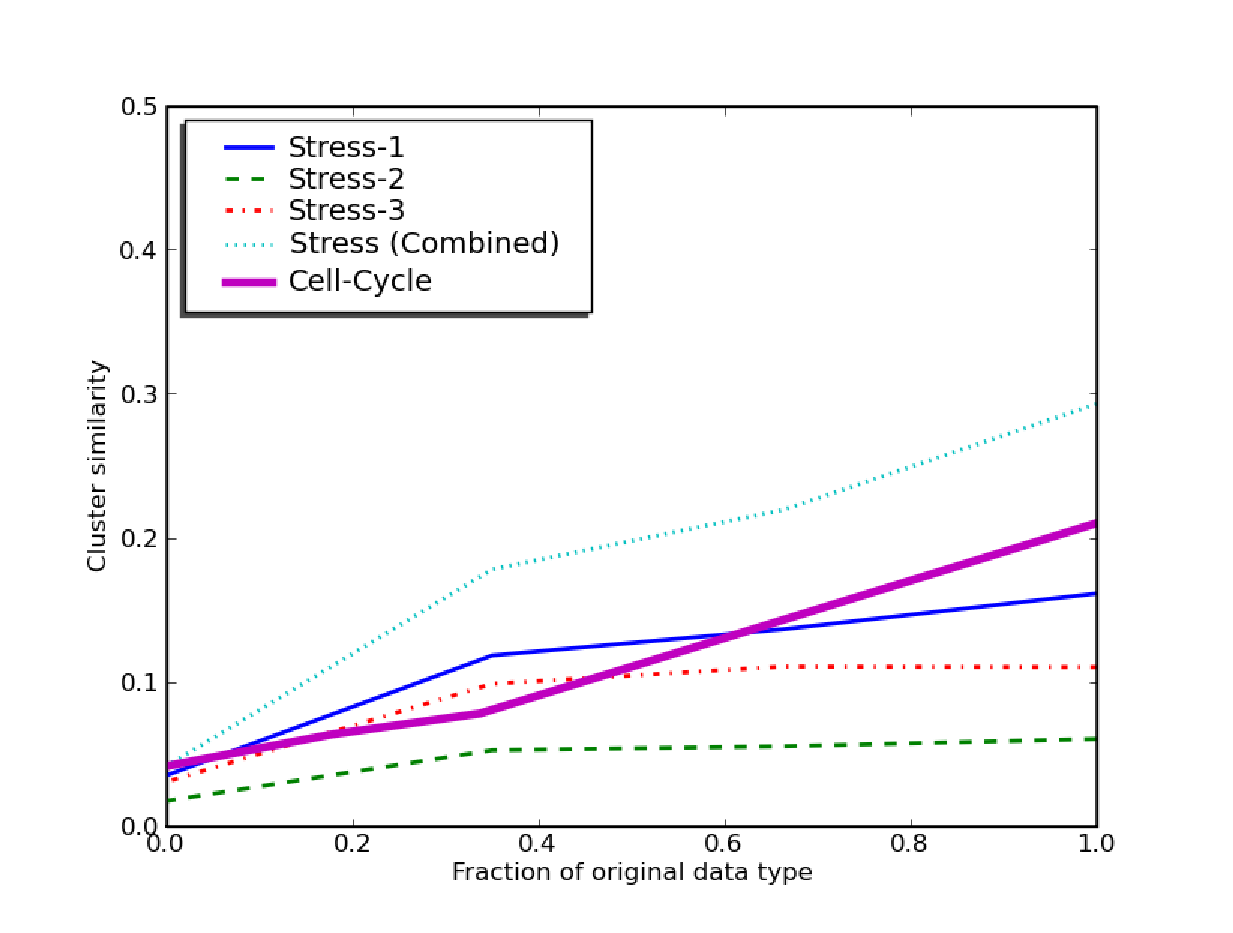
\includegraphics[scale=0.6]{chapter1/plot_unnorm.eps}
\caption{Full (non scale-normalized) data: Variation of cluster similarity with data homogeneity}
\label{graphs:all:unnorm}
\end{figure}

We also studied the variation of cluster similarity with the percentage of similar data as shown in Figures - (\ref{graphs:all:unnorm}, \ref{graphs:all:filtered} and \ref{graphs:all:norm}). For each mixed dataset, we calculated the fraction of original data type (e.g stress or cell-cycle) in the resulting mix. Similarity values were then plotted against these fractions. In all the figures, we see the general trend that as the fraction of the original datatype is increasing the cluster similarity values rises. We also observe that the combined datasets (both stress and cell-cycle) show a more consistent upward trend as compared to individual stress datasets. This is consistent with the observations we had in the earlier section and could be attributed to the dominance of stress data when mixed with other types. Figure-\ref{graphs:all:filtered} shows a gradually increasing trend though its not as smooth as Figure-\ref{graphs:all:unnorm} because of the increased dominance of the stress datasets when data is filtered. As seen from Figure-\ref{graphs:all:norm}, the general trend remains that similarity values increase with increasing fraction of similar data. These figures validate our hypothesis that we should be cautious towards integrating diverse datasets as they might be contributing to more noise and removing the original signals from the datasets. When we need to integrate different datasets, we should first compute their similarities and then only integrate similar ones while removing widely diverse ones.

\begin{figure}[t]\centering
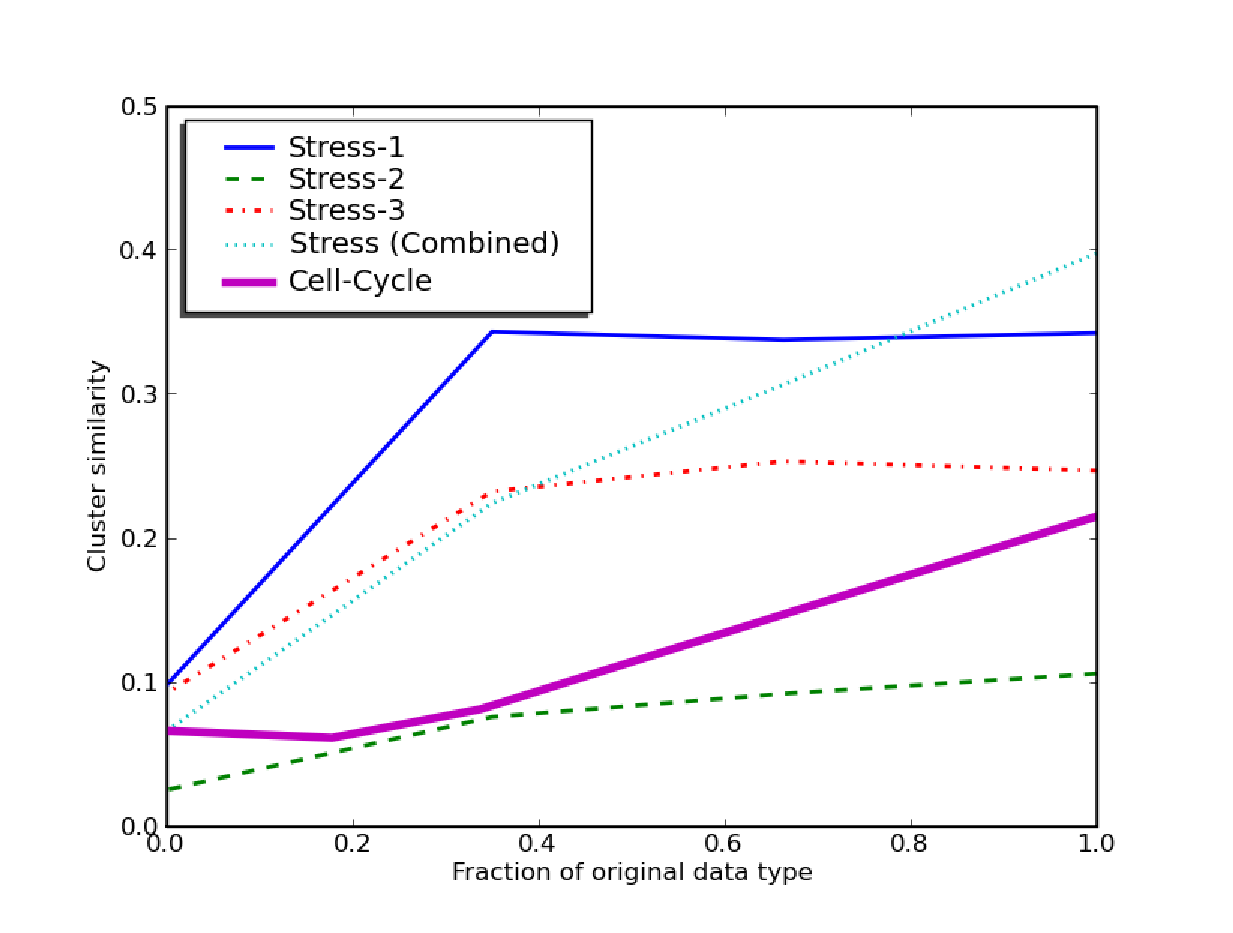
\includegraphics[scale=0.6]{chapter1/plot_filtered.eps}
\caption{Filtered (non scale-normalized) data: Variation of cluster similarity with data homogeneity}
\label{graphs:all:filtered}
\end{figure}

\begin{figure}[t]\centering
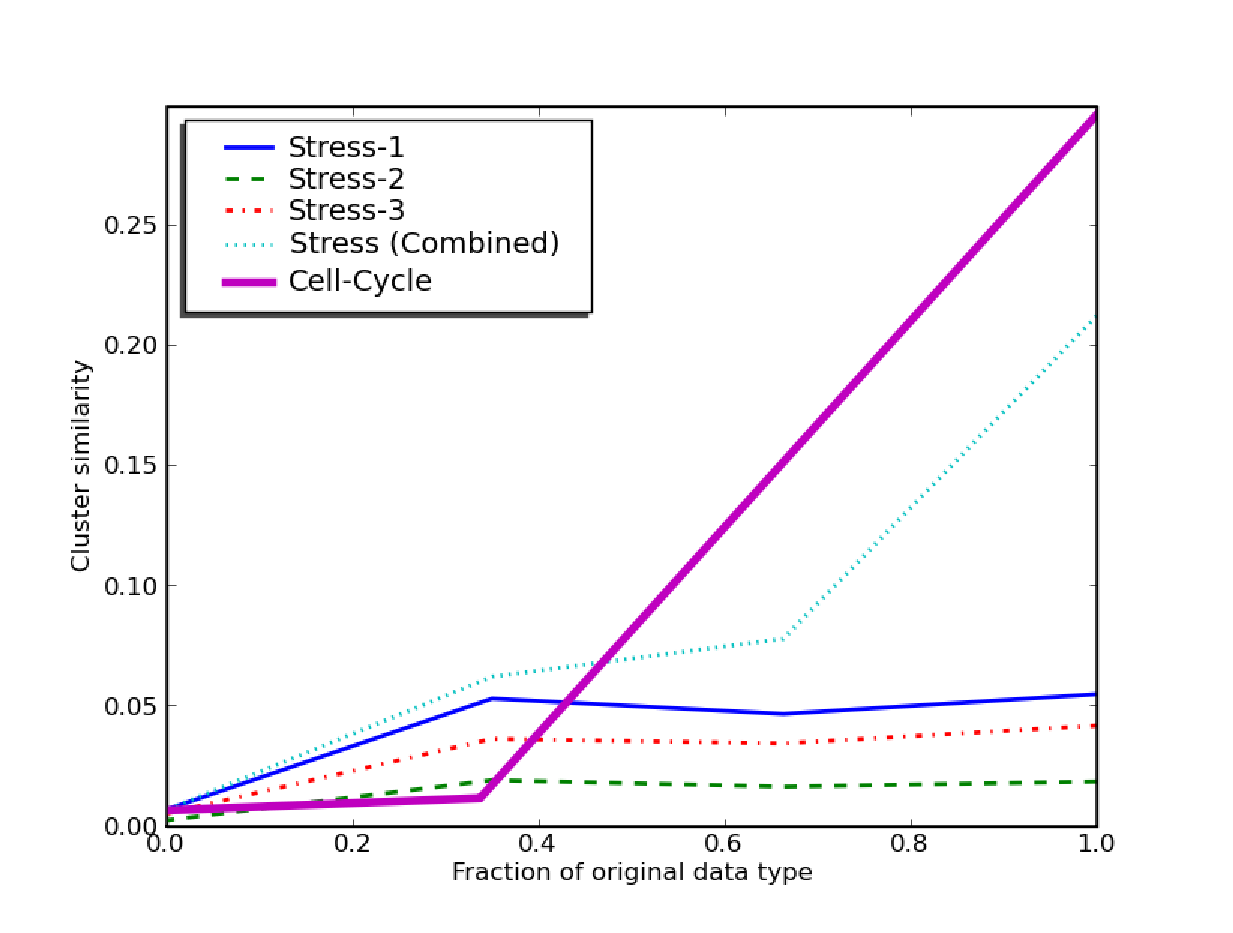
\includegraphics[scale=0.6]{chapter1/plot_norm.eps}
\caption{Full (scale normalized data): Variation of cluster similarity with data homogeneity}
\label{graphs:all:norm}
\end{figure}

\section{Discussion}
Learning the structure of genetic regulatory module networks has attracted a lot of attention in the past years. We saw a review of these techniques in Chapter-2. Recently, many researchers have focused on integrated approaches where they analyze a big compendium of microarrays gathered from various sources. \citet{hughes00functional} created a reference database or \textit{compendium} of whole-genome microarray data for yeast from 300 diverse mutations and chemical treatments under similar growth conditions. They used this to identify the pathways perturbed by an uncharacterized mutation by computing the similarity of expression of the uncharacterized mutation to the ones in the compendium. 

A similar compendium approach was followed by \citet{amos05integrative} who used data encompassing 1767 conditions from 60 different publications to find regulatory programs. The key difference from \citet{hughes00functional} is that while \citet{hughes00functional} had created the compendium from experiments under similar conditions in a single lab, \citet{amos05integrative} have used data from widely varying conditions. They followed the normalization methods suggested by individual authors to process the individual datasets. However, they did not do any combined (across all conditions) normalization to account for diversity across different datasets. This compendium was then used as a reference against which new data was compared. They used the SAMBA algorithm (refer Chapter-2) to transform all sources of information into generalized conditions (bi-partite graphs) and then analyzed them together. They also reported that stress data dominated their entire compendium because of extreme response of the organism to environmental stress.

\citet{myers2007context} have also addressed the problem of heterogeneous data integration. In research that was carried out after the publication of our research \citep{mishra2007effect}, they measured context-dependent variation for a wide variety of public genome data for yeast, including a large number of microarray, \ac{PPI} and sequence datasets. Not surprisingly, one of their finding is that the quality of datasets varies dramatically and the degree to which we should trust any dataset depends on the process we are interested in. They have proposed a Bayesian approach to perform context-sensitive integration of data for protein network recovery. 

 We have observed in both cluster similarities and KL divergences that stress data, which has much much higher levels of change in expression, has \textit{dominated} the final clusters when mixed with the cell-cycle data where the expression level changes are much lower. This is in line with the observations made by \citet{amos05integrative} in their large scale microarray integration study. They state that two opposite environmental stress responses dominate their entire compendium and the responses to stress are so strong and widespread that other, condition-specific regulatory programs are hard to detect without the combination of multiple studies and sensitive algorithms.  

One source of error in our results might be attributed to the fact that our similarity index is based on pairwise matches of genes in each sets and even though the adjusted Rand's index is one of the most stable indices for cluster similarity, yet it's not perfect. Another drawback of our \ac{KL} divergence computations between pairs of datasets is that we have assumed the covariance matrix is diagonal with no interactions among various genes. This assumption is a very naive one even though some researchers have found it to be quite useful \citep{ernstwit2004statis_microarrays} for practical purposes. The \ac{KL} divergence between two \textit{multivariate} Gaussian distributions $N_{0}(\mathbf{\mu}_{0},\Sigma_{0})$ and $N_{1}(\mathbf{\mu}_{1},\Sigma_{1})$ is given by \citep{kullback1997info},  
\begin{equation}
    KL(\mathit{N}_{0}\parallel \mathit{N}_{1})=\frac{1}{2}\ln |\Sigma_{1}\Sigma_{0}^{-1}|+\frac{1}{2}tr\Sigma_{1}^{-1}((\mathbf{\mu}_{0}-\mathbf{\mu}_{1})(\mathbf{\mu}_{0}-\mathbf{\mu}_{1})^{T}+\Sigma_{0}-\Sigma_{1})
\end{equation}
This involves estimating the covariance matrix. Because of the small number of experimental data available compared to the dimensionality of data, the resulting covariance matrix usually turns out to be singular and hence can not be inverted as required above. This forced us to use the independence assumption among genes which might have introduced some errors in KL divergence computations.

\section{Conclusion}
One of the original contributions of our work is that we have outlined an empirical technique to calculate functional similarity of datasets using the concept of cluster similarity. Based on its high correlation with underlying data distribution difference, we would like to propose it as an index of microarray dataset similarity. We have also showed that similarity values gradually fall with increasing fraction of dissimilar data. As argued in \citet{orph02thehuman}, all cellular regulatory mechanisms are very local in nature and trying to use a blind integrative approach is most likely going to prove futile in determining meaningful results. We have tried to establish this from a different point of view that as more diverse data-sets are merged then the similarity to individual data-sets (which have more local patterns) is reduced and the dominant ones overshadow the weaker signals. Therefore, before taking a blind integrative approach, much care should be taken to ensure that we mix only similar types of data. We should also be careful about the choice of normalization method. In our results we demonstrated that normalization can distort the data and affect the resulting clusters significantly.

The next chapter deals with data integration of a different type from that we have seen here. It deals with integration of different \textit{types} of data and details a framework for that.
 

\chapter{Semi-supervised Regulatory Module Discovery}
\begin{quote} ``Just as the constant increase of entropy is the basic law of the universe, so it is the basic law of life to be ever more highly structured and to struggle against entropy'' - \textit{Vaclav Havel}  \end{quote} 
 
While our previous chapter discussed the impact of data integration of the same type (microarrays), in this chapter we focus on the integration of the other type, where datasets of different types are used in a cooperative manner. Different datasets are not being merged \textit{literally}, but one is used to \textit{guide} the clustering of the other. We propose a type of clustering method with \textit{supervision} extracted from \textit{prior biological knowledge} in order to guide the process of clustering.

When a small amount of prior knowledge is available in the form of \textit{pairwise relationships} between genes, instead of simply using this knowledge for the external validation of the results of clustering, we can use it in order to guide the clustering process thus providing a limited form of supervision. We call these methods \textit{semi-supervised clustering} \footnote{This is different from Semi-Supervised Learning \citep{grira2005unsupsurvey} which is a class of machine learning techniques that make use of both labelled and unlabelled data for training. They are called semi-supervised because the available knowledge is far from being enough for fully supervised learning even in a transductive form.} because unlike supervised or constrained clustering \citep{bradley00constrained}, the final results of clustering is not required to enforce the constraints. The constraints act as guidelines and are enforced only if they are complementary to the data being clustered. For semi-supervised clustering to be profitable, the two sources of information, i.e., the similarity measure (used by all clustering methods) as well as the constraints available should not completely contradict each other.
In our novel formulation, named \acfi{SSSC}, supervision (prior knowledge) is provided in the form of binary constraints and clustering is done in the spectral space \citep{shi00normalized, ng2001onspectral}. The prior knowledge is derived from DNA binding data from ChIP-chip experiments, PPI data and known TF-gene interactions from a curated database. These are used to guide the process of clustering microarray data.

\section{Spectral Clustering}
The goal of any clustering is to partition a set of points into disjoint sets where the points within a partition are as similar as possible while points within different partitions are as dissimilar as possible. In this section, we discuss how spectral clustering achieves this objective. 
\subsection{Graph notations}
Given a set of data points, we can compute similarities between them using a suitable \textit{similarity function}. Given these similarities between the data points, a dataset can be represented as a \textit{graph} which is a set of \textit{vertices} and \textit{edges} connecting vertices \textit{(V,E)}. The vertices \textit{(V)} represent the data points while the edges \textit{(E)} represent the links between the data points. Usually a certain threshold of similarity value is chosen above which the edges are linked between data points. For \textit{weighted} graphs the edges also have the similarity values as \textit{weights}. Once we have this undirected weighted graph, the goal of a clustering algorithm is to partition it such that edge weights between the points \textit{within} a partition are high while the edge weights between points of \textit{different} partitions are low. We begin with some definitions.

Let $G = (V,E)$ be an \textit{undirected weighted} graph with vertices $V = {v_{1},\dots,v_{n}}$, edges $E= {e_{1},\dots,e_{n}}$ and each edge $e_{ij}$ between vertex $i$ and $j$  has a non-negative weight $w_{ij}$. The weights matrix $W = (w_{ij})_{i,j=1,\dots,n}$ is also known as the \textit{adjacency matrix} of this graph. For non existing edges, $w_{ij}=0$. The graph is assumed to have no self-edges, i.e., $w_{ii}=0$. In order to understand spectral clustering we need some more definitions for this graph.

The \textit{degree} ($d_{i}$) of a vertex $v_{i}$ is defined as
\[
d_{i} = \sum_{j=1}^{n}w_{ij}
\]

which intuitively is the row-wise sum for the respective row of the adjacency matrix. In the graph, this can also be understood in terms of sum of edge weights for that particular vertex. The \textit{degree matrix} $D$ is defined as the \textit{diagonal} matrix with the individual vertex degrees $d_{1}$, \dots, $d_{n}$ along the diagonal, everything else being $0$.

\subsection{Similarity matrices and graph Laplacians}
There are various ways of converting similarities between a given set of data points into a graph - both in choosing the similarity function to compute similarities 
among the data points as well as deciding about how to turn the similarity values into a graph.

A \textit{$\varepsilon$-neighbourhood} graph is obtained by joining edges between points whose similarity values are larger than  $\varepsilon$. 
Figure-\ref{fig:constraints_with_pval} shows two examples of such a graph using two different values of $\varepsilon$. A \ac{KNN} graph has edges between a 
point and $k$ other points that are most similar to it. This leads to a directed graph because the neighbourhood relation is not 
symmetric, i.e., $v_{a}$ might have $v_{b}$ as one of its k-nearest neighbours but the vice-versa might not be true. To convert this into an 
undirected one, we can either totally ignore the direction or take a more restrictive approach where two nodes are connected \textit{only} if 
both of them are \aclp{KNN} of each other. The latter type is also referred to as a \textit{mutual \acl{KNN} graph}.

A \textit{fully connected} graph is one where all pairs of points have positive similarity values and are connected. This leads to a denser 
graph in comparison to previous ones. While in the earlier ones, the local neighbourhood relationship was enforced with either a 
threshold ($\varepsilon$) or a maximum of $k$-neighbours, in a fully connected graph we have to choose a similarity function that should 
do this. For all our work, we have used the Gaussian similarity function which encodes this neighbourhood relation automatically. 
In this function, $exp \left( -\frac{{\parallel \textbf{x}-\textbf{x}^{'} \parallel}^{2}}{2\sigma^{2}}\right)$, $\sigma$ controls the width of 
the neighbourhood and $\textbf{x}$,$\textbf{x}^{'}$ represent the two variables between which similarity is being computed. The Gaussian similarity 
function is an exponential function, therefore depending on $\sigma$, the similarity falls non-linearly 
(exponentially) with increasing distance. This property makes it desirable to use where neighbourhood relations are important. Various 
other similarity functions for vector data are discussed in Chapter-\ref{chap_maxent}.

Spectral clustering is based on the \textit{Laplacian} matrix which has its origins in spectral graph theory \citep{chung1997spectralgraph}. There are various types of Laplacians. All of these assume that we have an undirected graph $G$ with positive weight matrix $W$ ($w_{ij} \geq 0$) and a corresponding degree matrix $D$. An \textit{unnormalized} Laplacian is defined as 

\[
	L = D-W
\] 
The matrix $L$ has the following properties
\begin{itemize}
    \item $L$ is always symmetric and positive semi-definite.
    \item $L$ has $n$ non-negative, real-valued eigenvalues $\lambda_{1}(=0) \leq \lambda_{2}\leq \dots \leq \lambda_{n}$. The number of smallest eigenvalues (=0), i.e., its multiplicity, corresponds to the number of connected components in the graph. 
\end{itemize}

There are two popular variants of the \textit{normalized} Laplacian. They are defined as

\begin{eqnarray}
	L_{symmetric} &=& D^{-1/2} L D^{-1/2} = I - D^{-1/2} W D^{-1/2} \label{eqn-lap_sym}\\
	L_{random walk} &=& D^{-1}L = I - D^{-1}W 
\end{eqnarray}
where $D^{-1/2}$ is the inverse square root of matrix $D$. Since $D$ is a diagonal matrix and the square root of a diagonal matrix D is formed by taking the square root of all the entries on the diagonal

\begin{displaymath}
    \mathbf{D^{\frac{-1}{2}}} = \begin{bmatrix} \frac{1}{\sqrt{d_{11}}} & 0 & \dots & 0\\
				 0 & \frac{1}{\sqrt{d_{22}}} & \dots & 0\\
                                 \vdots & \vdots & \ddots & \vdots\\
				 0 & 0 & \dots & \frac{1}{\sqrt{d_{nn}}}\\
                 \end{bmatrix}
\end{displaymath}
Like the unnormalized Laplacian, the normalized ones are also always symmetric and positive semi-definite. They too have non-negative, real-valued 
eigenvalues $\lambda_{1}(=0) \leq \lambda_{2}\leq \dots \leq \lambda_{n}$ and the multiplicity of the smallest eigenvalue is the number of 
connected components in the graph. Laplacians could be interpreted as \textit{gradients} on graphs and it is related to differential geometry. 
\subsection{Graph clustering}
As seen earlier, given a set of data points, a similarity function can be used to calculate the pairwise similarities among them, resulting in a similarity matrix. Given its graph representation, the clustering can be defined as a \textit{graph partitioning} problem where the edges between the points of the \textit{same} cluster have high weights while the edges between points belonging to \textit{different} clusters have low weights. Before we discuss the algorithm in detail, we discuss the general problem of graph clustering and its relation to spectral clustering. 

We know that the key objective of clustering is to find sets of points that are \textit{maximally similar to each other within a set} 
and \textit{maximally dissimilar to points in other sets}. If we have a similarity graph, as discussed earlier, the problem can be restated to 
find a partition of the given graph such that the edges between points within a partition have higher weights as compared to edges 
between points in different partitions. Graph clustering or partitioning is an old problem 
and has been exhaustively studied \footnote{For a good review, see \cite{schaeffer1997graphclustering}}. Spectral clustering can be derived as an approximation to the graph partitioning objectives \citep{luxberg2006tutorial_spectral}. Before we start, we need some definitions.

If we have two disjoint partitions A, B then 
\[
	Cut(A,B) = \sum_{i \in A,j \in B}w_{ij}
\] 
	
So, if we have a graph G with adjacency matrix $W$, then we can construct a partition by solving the \textit{min-cut} problem, which can be understood 
as choosing the partitions $A_{1},\dots,A_{k}$ such that we minimize the following cut.

\[
	Cut(A_{1},\dots,A_{k}) = \sum_{i=1}^{k}Cut(A_{i},\bar{A}_{i})
\] 
where \={A} is the complement of $A$. While theoretically it can be solved, yet in practice it may yield clusters of 
size 1 (trivial clusters), which is not usually the goal of clustering. We want clusters that are \textit{reasonably} big. This is 
specified in terms of two popular \textit{objective functions} namely \textit{RatioCut} and normalized cut or \textit{NCut}.

\begin{eqnarray}
    RatioCut(A_{1},\dots,A_{k}) &=& \sum_{i=1}^{k}\frac{Cut(A_{i},\bar{A}_{i})}{|A_{i}|} \\
    NCut(A_{1},\dots,A_{k}) &=& \sum_{i=1}^{k}\frac{Cut(A_{i},\bar{A}_{i})}{vol(A_{i})}
\end{eqnarray}

While in RatioCut the normalizing factor is the $|A_{i}|$, which is the total number of vertices (points) in the $i_{th}$ partition, in NCut, the normalizing factor is $vol(A_{i})$ which is the sum of all edge weights in the partition. The role of this normalizing factor is to make the partition \textit{balanced} as measured by number of vertices or sum of edge weights. Even though the formulation is simple and elegant, it is an NP-hard\footnote{NP-hard (nondeterministic polynomial-time hard) is a class of problem in computational complexity theory} problem. The spectral clustering algorithm is a way to solve a relaxed version of these objective functions. 

Another way to understand this is that in both RatioCut and NCut, the numerator tries to achieve the objective of making different clusters as dissimilar to each other as possible, i.e., minimize the between cluster similarity. This is one half of the key requirement of any clustering algorithm's objective. The other half is that the within-cluster similarity should also be maximized. In other words $\sum_{i,j \in A}w_{ij}$ and $\sum_{i,j \in \bar{A}}w_{ij}$ should be maximized. Let's see how this is satisfied in each of the objective functions. 

\begin{eqnarray}
 \sum_{i,j \in A}w_{ij} &=& \sum_{i \in A, j \in A \cup \bar{A}}w_{ij} - \sum_{i \in A, j \in \bar{A}}w_{ij} \\
                        &=& vol(A) - Cut(A,\bar{A})	 
\end{eqnarray}

We can see that NCut satisfies this by maximizing $vol(A)$ and minimizing $Cut(A,\bar{A})$. RatioCut doesn't lead to this objective. As shown in \citet{luxberg2006tutorial_spectral}, relaxing NCut leads to using the \textit{normalized} Laplacian in spectral clustering while relaxing RatioCut leads to the use of \textit{unnormalized} Laplacian. Therefore, normalized spectral clustering satisfies both the key clustering criteria while unnormalized spectral clustering only implements the first criteria. One key point to note is that there is no guarantee on the quality of the clustering solution of the relaxed problem compared to the exact solution. 

\subsection{Algorithm explanation}
Spectral clustering is a technique in which the eigenvectors of the Laplacian matrix (which is derived from the \textit{similarity} matrix) corresponding to 
the smallest eigenvalues are used to derive a clustering of the given data points. The methods are called spectral, because 
they make use of the \textit{spectrum}\footnote{The set of eigenvectors of the normalized Laplacian matrix is usually called 
the \textit{spectrum} of the Laplacian (or the spectrum of the associated graph)} of the graph. It has been applied to diverse 
domains, e.g. image segmentation \citep{shi00normalized, weiss1999segmentation} and bioinformatics \citep{speer05spectral}. Most spectral clustering algorithms 
can be considered to have three stages:
\begin{description}
    \item[Normalization] This consists of computing the similarity matrix from the raw data using a suitable similarity function. We call this the \textit{normalization} step because different types of data (vector, graph or string) get converted to a common format (similarity matrix).
    \item[Eigen Decomposition] This consists of computing the eigenvalues and the corresponding eigenvectors of the similarity matrix. This step could be considered as the mapping of original data to the spectral domain.
    \item[Clustering] This step consists of using a traditional clustering algorithm (usually k-means) to cluster the vectors in the spectral domain.	
\end{description}
Different spectral clustering algorithms differ in the number of eigenvectors used (single or many) as well as the type of Laplacian 
used (unnormalized or normalized). \citet{verma2003comparison} did a systematic comparison of different popular 
spectral \citep{shi00normalized, ng2001onspectral, meila2000learning} and traditional clustering algorithms on artificial as well as 
real-world datasets. They report that spectral methods are more stable to noise than other tested algorithms. 
Both \citet{shi00normalized} and \citet{meila2000learning} have used the $L_{random walk}$ normalized Laplacian while \citet{ng2001onspectral} 
have used the $L_{symmetric}$ normalized Laplacian. Apart from this, there is no major difference between the techniques of all these algorithms. 
Since \citet{verma2003comparison} did not find significant differences among the two normalized Laplacians, we have used the 
algorithm by \citet{ng2001onspectral} which is the most recent one. This algorithm is described in Algorithm-\ref{alg:spectral_clustering}.
\begin{algorithm}
\caption{Spectral clustering}
\label{alg:spectral_clustering}
\begin{algorithmic}[1]
\REQUIRE Dataset ($X$), number of clusters ($k$) 

\STATE Calculate the symmetric similarity matrix $K_{n \times n}$  using Gaussian similarity function  $K_{ij}=exp \left( -\frac{{\parallel x_{i}-x_{j} \parallel}^{2}}{2\sigma^{2}}\right)$ if $i\neq j$, and set $K_{ii}=0$. 

\STATE Calculate normalized Laplacian $L'=D^{-1/2}KD^{-1/2}$ where D is the diagonal matrix with $d_{jj}=\sum_{i}d_{ji}$ 

\STATE Find the eigenvectors $v^{1},v^{2},\dots,v^{k}$ corresponding to the largest k eigenvalues of $L'$. 

\STATE Use these k eigenvectors as columns to get $V_{n \times k}$. 

\STATE Normalize the row to have unit norm, i.e., $U_{n \times k}$ such that $u_{ij}= v_{ij}/(\sum_{k}{v_{ik}^{2}})^{\frac{1}{2}}$

\STATE Cluster the points representing the rows of this matrix $(u_{i})_{i=1,...,n}$ using k-means algorithm into k clusters, $C_{1},C_{2},\dots,C_{k}$.  

\STATE Output clusters $A_{1},A_{2},\dots,A_{k}$ such that $A_{i}=\{x_{j}|u_{j}\in C_{i}\}$. This assigns the original point $x_{j}$ to cluster $A_{i}$ if $u_{j}$ is in cluster $C_{i}$. 

\end{algorithmic}
\end{algorithm}

In the previous description of this algorithm, we had mentioned that the eigenvectors corresponding to the smallest eigenvalues are used. However, in the step-3 of algorithm, we are proposing to take the eigenvectors corresponding to the largest k eigenvalues. This is because here we are using the Laplacian $L'$ instead of the form $L_{symmetric=}I-L'$ described earlier (refer eqn-\ref{eqn-lap_sym}). This changes the eigenvalues from $\lambda_{i}$ to $1-\lambda_{i}$.

To summarize the functioning of this algorithm: it changes the representation of the data points from the original space to the spectral space after the various steps (1-5) of transformation as shown in Algorithm-\ref{alg:spectral_clustering}. After that, any clustering algorithm can be used to cluster the data points. The reason for this transformation is that it allows better identification of non-linear clusters. Non-linear patterns are very hard to identify using traditional clustering methods but after the spatial transformation it becomes trivial to find them. For a detailed understanding of why this algorithm works, refer \citet{ng2001onspectral}. 

Spectral clustering is very appealing because it yields a very standard linear algebra problem for which there are various efficient solvers (algorithm implementations) already available. It can be implemented for even large datasets if the similarity matrix is sparse. Unlike traditional clustering algorithms like k-means, there are no issues of dependency on starting point or getting stuck in local optimum. On the flip side, choosing the right similarity function and its parameters is non-trivial.

\section{Datasets and Our Algorithm} \label{chap2:sec:materials}

\subsection{Microarray datasets}
We have used two popular microarray datasets on which the clustering is carried out, both of them based on experiments done on yeast (Saccharomyces cerevisiae). The dataset by \citet{gasch00genomicexpn} was obtained by exposing yeast to diverse environmental (stress) conditions such as temperature shocks, hydrogen peroxide, the superoxide generating drug menadione, the sulfhydryl-oxidizing agent diamide, the disulfide-reducing agent dithiothreitol, hyper and hypo-osmotic shock, amino-acid starvation and nitrogen source depletion. More than 900 genes showed drastic response to these environmental changes. We selected only those genes that displayed a change of three fold in \textit{at least one experiment}. There were 1246 genes fulfilling this criterion. The assumption behind this selection strategy is that the majority of genes which do not show much change in their expression levels during a process are unrelated to it.

The second microarray dataset was based on cell-cycle experiments by \citet{spellman98comprehensive} where the objective was to identify yeast genes which were involved in cell-cycle regulation. This was achieved using DNA microarrays synchronized using three independent methods: $\alpha$ factor arrest, elutriation, and arrest of a cdc15 temperature sensitive mutant. Again, we selected only those genes that displayed a change of two fold in \textit{at least one experiment}. There were 1732 genes fulfilling this criterion. The reason why we only filtered for two fold change is because stress leads to a much more widespread expression change across the genome. Therefore, the number of genes that show change at two fold are too high. On the other hand, expression level changes are not that severe in a normal cell-cycle study. So, the number of genes at two fold change are not that high.

In both the datasets, for data imputation we use the R \textit{impute} package which uses \textit{k-nearest neighbour} algorithm to impute missing values. It uses a Euclidean distance metric for finding nearest neighbours. We used the $log_{2}$ of the ratio of the mean of Channel 2 (experimental expression) to the mean of Channel 1 (control expression) since this is likely to create a Gaussian distribution \citep{ernstwit2004statis_microarrays}.

For the experiments where we combined microarray with DNA-binding data, we needed to do other steps of pre-processing. We found the list of genes responsible for the TFs that were tested for binding. Then we ensured that our microarray dataset had those. The reasoning behind this is that some of them might be missing after the filtering step. In such a case, they were extracted from the original unfiltered dataset and incorporated in the final filtered one. The number of these is small compared to the total number of genes and we didn't want to loose any of them.

\subsection{DNA-binding dataset}
One of the datasets which we have used to guide the clustering process is the DNA-binding dataset on yeast \citep{harbison04transcriptional}. It was created using genome-wide 
location analysis techniques to determine the genomic occupancy of 203 DNA-binding transcriptional factors. In this dataset, the likelihood of a particular TF 
binding to the promoter region of another gene is reported in terms of a confidence value (p-value). A lower p-value indicates higher confidence. In order to extract binary 
constraints from this dataset, we need some threshold on these reported p-values of interactions. We investigated a range of p-value cut-offs, each corresponding to a 
certain set of constraints. This was to study the impact of \textit{number} and \textit{quality} of constraints on the biological significance of clustering. 
Since these are experimentally determined, we consider them as a more reliable evidence of genetic interaction. After extracting the constraints, we use them for 
guiding the clustering process. 

As stated, we used the p-value thresholds to convert the confidence value data into binary constraints. For example, if the p-value threshold is  
0.001 then all values below this are considered as \textit{definitely bound} and hence assigned a value of 1. The rest are assigned 0 (not bound). A significant point to 
note is that these p-value cut-offs have a dual role. They determine the number of constraints as well as the quality of constraints. As the p-value cutoff is increased, 
the number of constraints increases, but a higher p-value also indicates lower confidence, hence the quality of the constraints falls. Table-\ref{tab:no_constraints} shows 
the number of constraints corresponding to various p-value cut-offs. Figure-\ref{fig:constraints_with_pval} shows these constraints graphically where we can see that the 
graph density is very high at p=0.001 compared to at p=0.0001. 

Our constraints are transformed into a $m \times n $ matrix where $m$ is the number of genes and $n$ is the number of TFs. This constraints matrix is used to modify 
the similarity matrix that we obtain from the microarray data as discussed in Section-\ref{sec:sssc}.

\begin{figure}[p]
  \begin{center}
   \subfigure[Constraints at p=0.0001]{\label{fig:graph_constraints_0.0001}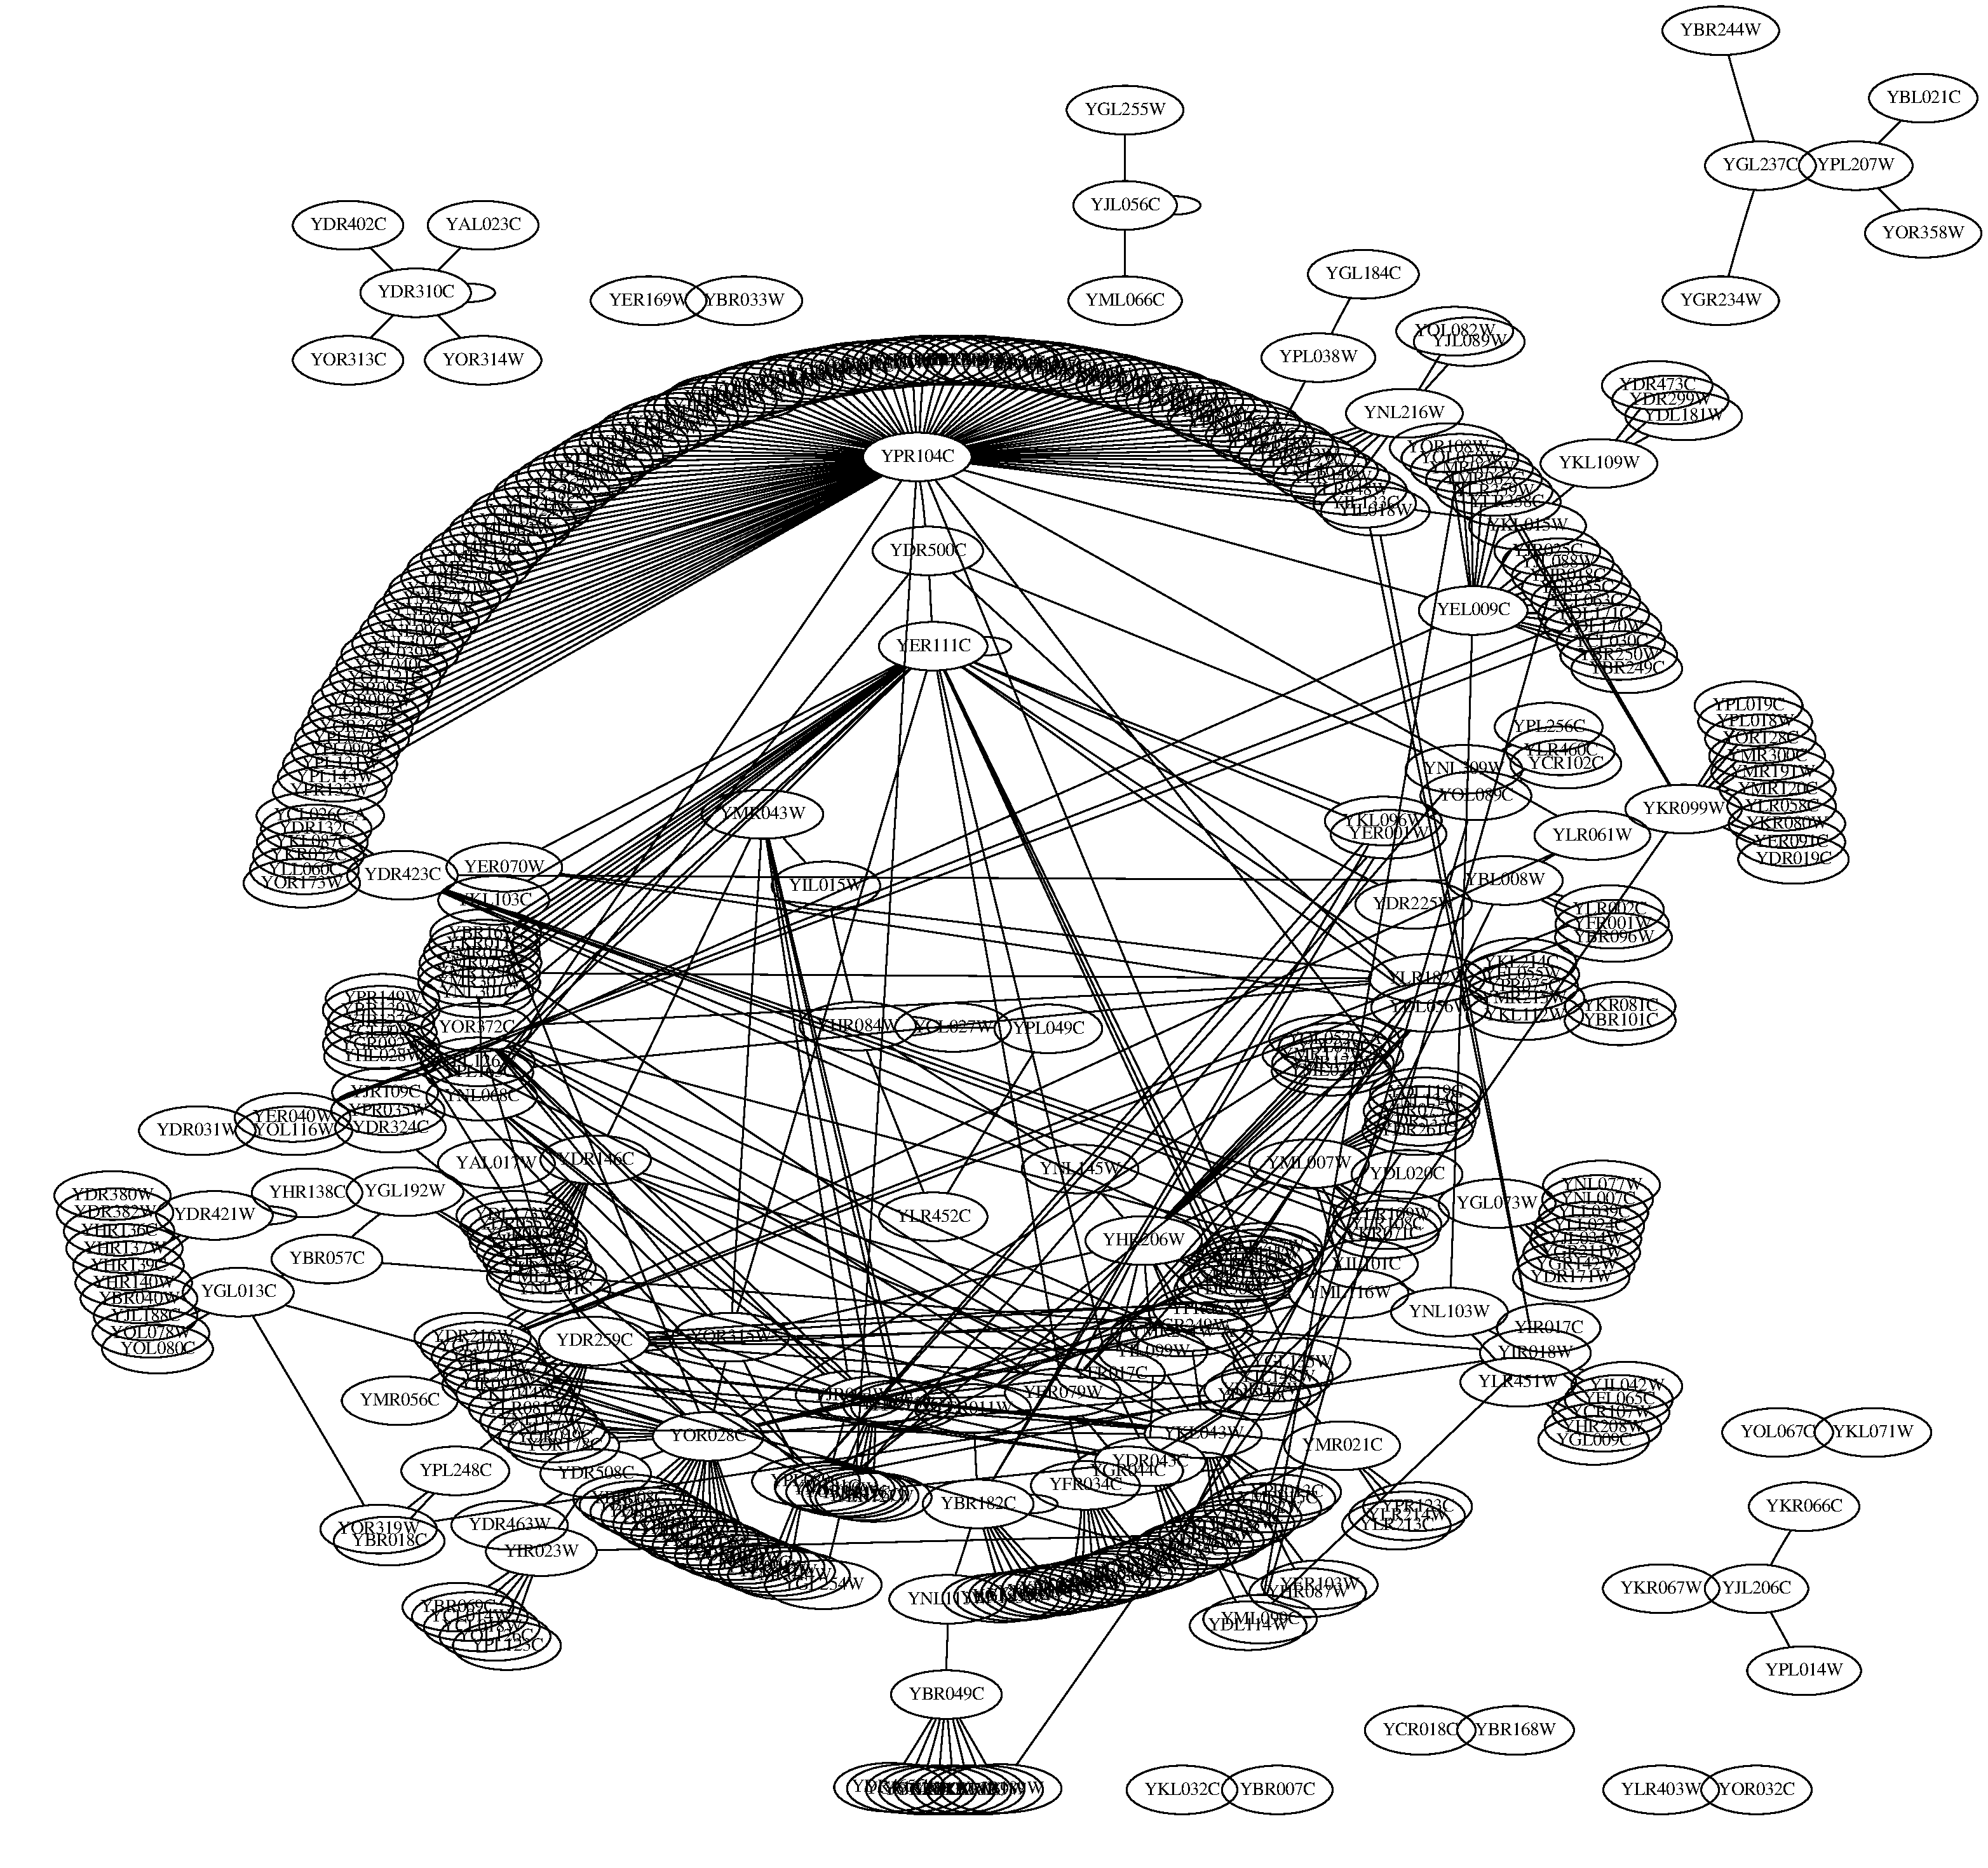
\includegraphics[scale=0.2]{chapter2/graph_0.0001.eps}}
   \subfigure[Constraints at p=0.001]{\label{fig:graph_constraints_0.001}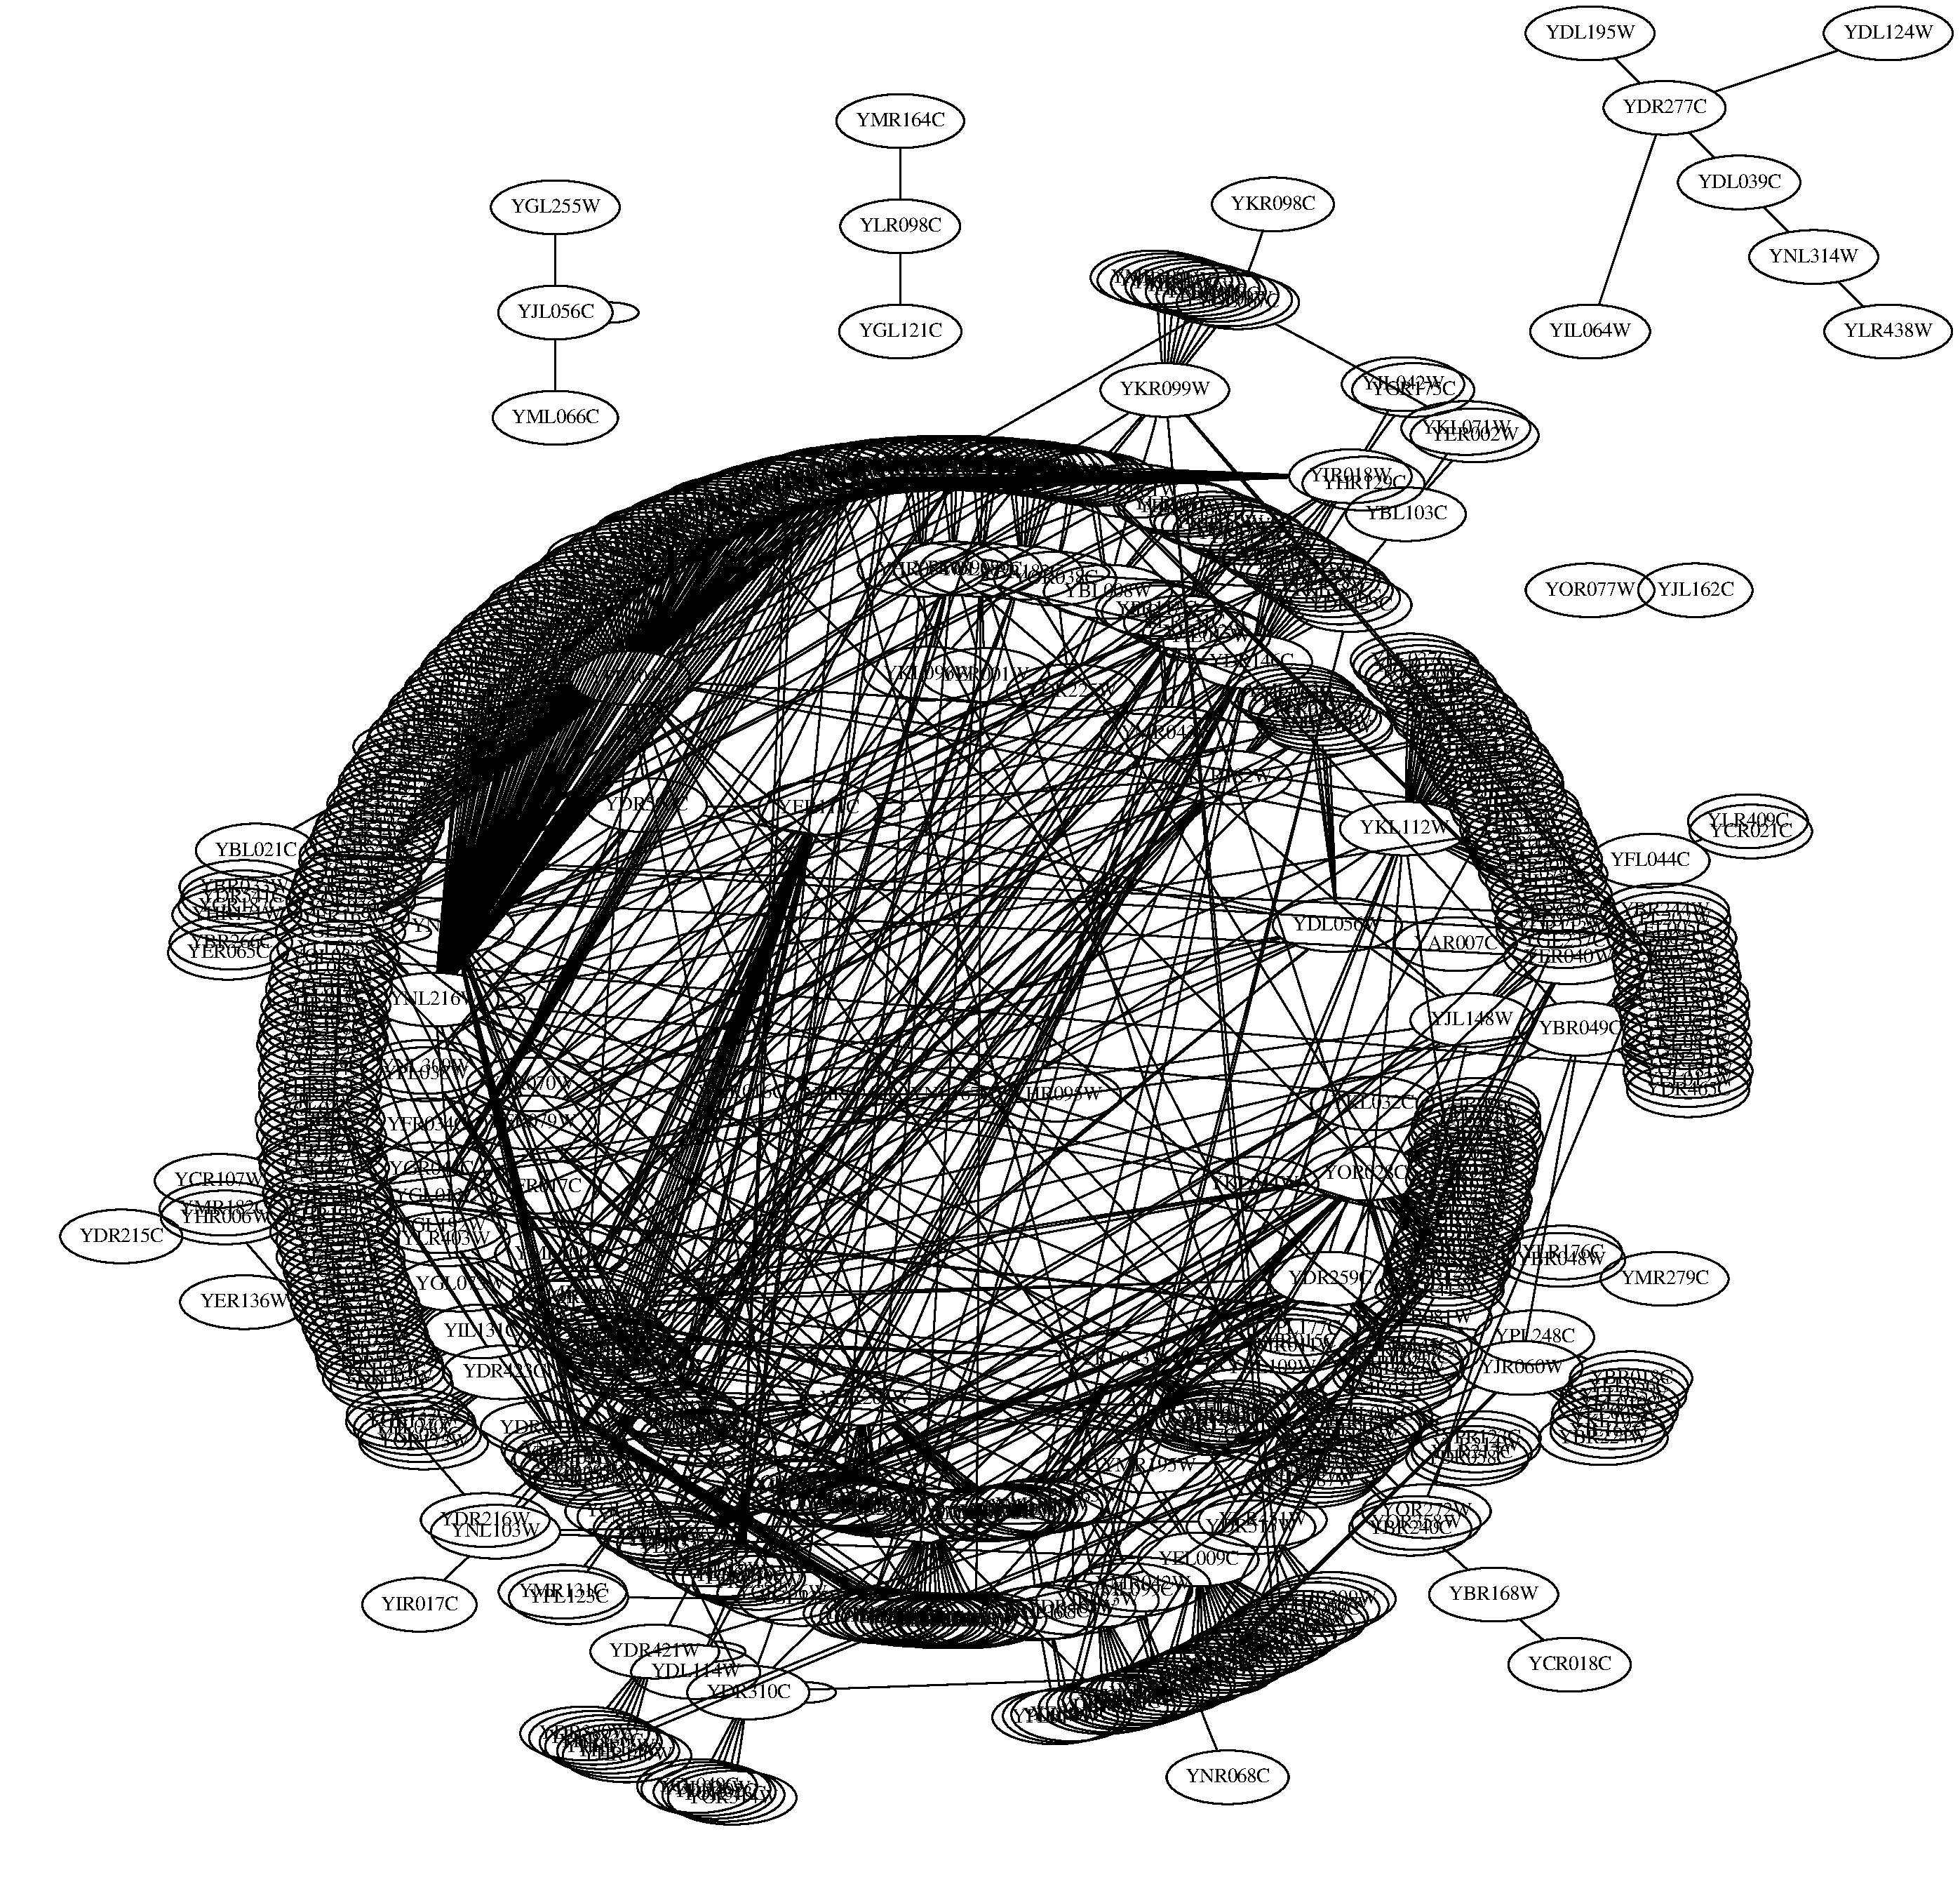
\includegraphics[scale=0.2]{chapter2/graph_0.001.eps}}

  \end{center}
\caption{Constraints derived from DNA-binding dataset at various p-value cutoffs}
\label{fig:constraints_with_pval}
\end{figure}

\begin{table}
\centering
\begin{tabular}{|c|c|c|c|}
\hline
p-value & \multicolumn{3}{|c|}{Number of Constraints} \\ \cline{2-4}
& All Genes & Common Genes (Stress) & Common Genes (Cell-cycle)\\
\hline
0.0001 & 2061  & 544   & 681\\
0.0005 & 3436  & 846   & 1032\\
0.001  & 4358  & 1053  & 1288\\
0.005  & 8562  & 1959  & 2442\\
0.01   & 12455 & 2776  & 3505\\
0.05   & 35917 & 7407  & 9713\\
0.1    & 63531 & 12579 & 17055\\
\hline 
\end{tabular}
\caption[Number of constraints from DNA-binding dataset at various p-value thresholds]{Number of constraints from DNA-binding dataset at various p-value thresholds. As the p-value 
cutoff is increased, the number of constraints increases.}
\label{tab:no_constraints}
\end{table}

\subsection{PPI dataset}
Another source of constraints is the popular PPI dataset from MIPS Comprehensive Yeast Genome Database (CYGD) \citep{Gueldener2006MPact}. It has been called a gold standard 
because of its quality and comprehensiveness \citep{yu2004annotation}. This dataset has information related to the proximity of proteins in yeast based on more than 
15446 protein-protein interaction records (9200 physical, 6400 genetic) which was compiled manually from the literature (3680 from single experiments) and published large-scale 
experiments. In addition to this, 268 manually extracted protein complexes as well as 783 complexes derived from large-scale experiments results in 87000 putative 
binary interactions. 

\subsection{TF-gene interactions dataset} \label{yeastract-db}
We also derived constrains from an independently curated database of known TF-gene interactions known as YEASTRACT(Yeast Search for Transcriptional Regulators And Consensus Tracking). 
YEASTRACT\footnote{interactions file created on 25/12/2008} \citep{Teixeira06yeastract} is a curated repository of 34471 regulatory associations between transcription factors and 
target genes in Saccharomyces cerevisiae, based on more than 1000 bibliographic references. In this database, the curators consider interaction to have occurred when there is change in the expression of the target gene owing to the deletion (or mutation) of the transcription factor-encoding gene. They also consider evidence based on TF binding to the promoter region of the target gene based on band-shift, footprinting or chromatin immunoprecipitation assays. They also describe potential associations but we have not considered them as we wanted to stick to known facts. 

\subsection{Semi-supervised spectral clustering} \label{sec:sssc}
We propose a semi supervised form of the spectral clustering method, which is detailed in Algorithm-\ref{alg:semi_sup_spectral_clustering} and shown in Figure-\ref{fig:semi_sup_spectral_clustering}. We are clustering microarray data, hence the genes can be considered the variables and their pairwise similarity values are calculated using a Gaussian affinity function. We have chosen this similarity function because it naturally encodes the local neighbourhood property and its value falls rapidly as the pairwise dissimilarity increases. Once we have this similarity matrix, we use the constraints derived from our secondary datasets to modify it. Since our constraints already encode our belief about potential interactions, we set each value in the similarity matrix to 1 (maximum similarity) if there is a 1 in the corresponding constraints matrix. All other values are left unchanged as we have no information regarding them. The idea behind changing the values to represent maximum similarity is to give the algorithm the maximum incentive to keep them in the same cluster. The resulting matrix is the final similarity matrix that we use for spectral clustering (Steps 3-7). We have used the algorithm suggested by \citet{ng2001onspectral}. The implementation was done in R using readily available libraries for linear algebra. 

We calculate the normalized Laplacian and then find its eigenvalues. If we believe there are $k$ clusters then eigenvectors corresponding to the $k$ smallest eigenvalues are chosen. If we arrange these $k$ eigenvectors column-wise then we end up with a $n \times k$ matrix. Each row of this matrix is then normalized to have unit norm. Then we cluster the rows using the k-means clustering algorithm. For all these integrated matrices, the k-means clustering of the eigenvectors was started from fixed centres. These 50 centres, each representing a cluster, were the genes encoding the TFs that had the highest numbers of DNA-interactions in the DNA-binding dataset. The idea behind this choice is to guide the clustering process to start from meaningful positions rather than random ones. Again, in step-4 of algorithm, we are proposing to take the eigenvectors corresponding to the largest k eigenvalues. This is because here we are using the Laplacian $L'$ instead of the form $L_{symmetric=}I-L'$ described earlier (refer eqn-\ref{eqn-lap_sym}). This changes the eigenvalues from $\lambda_{i}$ to $1-\lambda_{i}$. 

\begin{algorithm}
\caption{Semi-supervised spectral clustering}
\label{alg:semi_sup_spectral_clustering}
\begin{algorithmic}[1]
\REQUIRE Dataset ($X$), number of clusters ($k$) 

\STATE Calculate the symmetric similarity matrix $K_{n \times n}$  using Gaussian similarity function  $K_{ij}=exp \left( -\frac{{\parallel x_{i}-x_{j} \parallel}^{2}}{2\sigma^{2}}\right)$ if $i\neq j$, and set $K_{ii}=0$. 

\STATE Use the constraints to modify $K, K_{final}=K \oplus C$ where C is the constraints matrix. $K \oplus C$ implies that we set $K_{i,j}=1$ where $C_{i,j}=1$. 

\STATE Calculate the normalized Laplacian $L'=D^{-1/2}K_{final}D^{-1/2}$ where D is the diagonal matrix with $d_{jj}=\sum_{i}d_{ji}$ 

\STATE Find the eigenvectors $v^{1},v^{2},\dots,v^{k}$ corresponding to the largest k eigenvalues of $L'$. 

\STATE Use these k eigenvectors as columns to get $V_{n \times k}$. 

\STATE Normalize the rows to have unit norm, i.e., $U_{n \times k}$ such that $u_{ij}= v_{ij}/(\sum_{k}{v_{ik}^{2}})^{\frac{1}{2}}$

\STATE Cluster the points representing the rows of this matrix $(u_{i})_{i=1,...,n}$ using k-means algorithm into k clusters, $C_{1},C_{2},\dots,C_{k}$.  

\STATE Output clusters $A_{1},A_{2},\dots,A_{k}$ such that $A_{i}=\{x_{j}|u_{j}\in C_{i}\}$. This assigns the original point $x_{j}$ to cluster $A_{i}$ if $u_{j}$ is in cluster $C_{i}$. 

\end{algorithmic}
\end{algorithm}

\begin{figure*}[tp]
\centering
\scalebox{1.0}{
\begin{pspicture}(0,0)(16,12)
\psframe[framearc=0.1,linewidth=0.5mm](0,0)(16,12)

\rput(8.5,9.5){\Rnode{B}{$\begin{pmatrix}
1 & 1 & 0 & 0\\
0 & 0 & 0 & 1\\
1 & 0 & 1 & 1\\
0 & 0 & 0 & 0\\
\end{pmatrix}
$}}
\rput(5.1,9.5){\MyBox*[linecolor=lightgray]{4}{2}{Constraints Matrix derived from supervision sources}}

\pcline{->}(8.5,7)(8.5,5)
\pcline{->}(2.5,3.8)(3.5,3.8)

% microarray box and text
\rput(0.4,2.5){\Rnode{A}{\psgrid[gridwidth=0.02,subgridwidth=0.02,gridlabels=0.0pt,subgriddiv=4](0,0)(0,0)(2,3)}}
\rput(1.5,5.7){Conditions}
\rput(1.8,1.2){Microarray Data}
\rput{-270.0}(0.2,3.5){\rput(0,0){Genes}}

\rput(5.35,4){\Rnode{C}{$\begin{pmatrix}
0.2 & 0.5 & 0.6 & 0.2\\
0.3 & 0.3 & 0.3 & 0.3\\
0.2 & 0.4 & 0.6 & 0.2\\
0.7 & 0.4 & 0.3 & 0.6\\
\end{pmatrix}
$}}
\rput(5.5,1.2){Affinity Matrix}

\pcline{->}(7.6,3.8)(9.75,3.8)\nbput{\MyBox*[linecolor=lightgray]{3}{1}{set $A_{i,j}=1$ where $C_{i,j}=1$ }}
\rput(12,4){\Rnode{D}{$\begin{pmatrix}
1 & 1 & 0.6 & 0.2\\
0.3 & 0.3 & 0.3 & 1\\
1 & 0.4 & 1 & 1\\
0.7 & 0.4 & 0.3 & 0.6\\
\end{pmatrix}
$}}
\rput(12,1.2){Final Matrix}

\pcline{->}(14,3.8)(14.7,3.8)
\rput{-270.0}(15,3.8){\rput(0.1,-0.3){\MyBox*[linecolor=lightgray]{4}{1}{Spectral Clustering}}}

\end{pspicture} 
}

\caption{Visual representation of Semi-supervised spectral clustering}
\label{fig:semi_sup_spectral_clustering}
\end{figure*}

\subsection{Toy dataset explorations} \label{chap2:sec:spirals_dataset}
The semi-supervised problem can be stated as - there is a real distribution of data points that have certain pairwise similarities and an ideal clustering can be derived from it. 
We want to recover a clustering as close to the ideal one based on observing some noisy datasets and some facts (acting as constraints in our setup) that are known to us. Before we start work on real datasets 
we are going to show that semi-supervised clustering indeed is able to leverage external information in the form of pairwise constraints in order to better the clustering results. 

In order to do this, we take a toy dataset with non-linear patterns (points belonging to two classes are present in the form of two spirals) as seen in Figure-\ref{fig:spirals_original}. This data-set consists of two concentric clusters (300 points belonging to two classes) and was chosen because this is a specially 
hard problem on which many most traditional clustering algorithms fail. It also shows the effectiveness of spectral clustering in finding non-linear clusters which is not possible with 
traditional clustering algorithms. To represent the known facts or constraints, we extract some random constraints from it. Then to represent a noisy dataset, we skew the $\sigma$ with which pairwise similarities are computed from its optimum value to some random non-optimum value. After this, we study if the addition of progressively increasing quantities of the known relationships (constraints) improves the cluster quality of the noisy dataset.
We have used five-fold validation to study the effectiveness of our algorithm. So, in every run of the experiment 80\% of the data acts as training data 
while remaining 20\% is test data. The exact steps are detailed below 

\begin{enumerate}
 \item Take the spirals dataset which has two classes visually represented as red and black points as seen in Figure-\ref{fig:spirals_original}. 
We compute the optimal $\sigma$ with which to compute pairwise similarities by finding the least cumulative sum across all the clusters of sum of squared 
distance of all points in a cluster from its cluster centre as shown in Equation:\ref{maxent:eqn:withinss}. With this optimal $\sigma$ we compute the similarity matrix. 
We also generate a noisy version of it by changing the $\sigma$ to a random non-optimal value with which pairwise similarities are computed. 
The results of clustering with optimal and non-optimal $\sigma$ values are shown in Figures-\ref{fig:spirals_original} and \ref{fig:spirals_no_constraints} respectively.
 \item From the original dataset, we generate all possible pairs between all the points in each of the two classes respectively. Out of all these pairs, according to 5-fold cross validation procedure, take 4 parts as the training set and the remaining one as the testing set.
 \item Draw \textit{5} pairs of constraints from the training set randomly.
 \item Apply these pairwise constraints to the non-optimal similarity matrix, i.e., set the pairwise similarity of these data points to 1. Cluster it using spectral clustering.
 \item Compute the similarity between the resulting cluster and the original clustering using modified Rand's index (discussed in Chapter-3).
 \item Repeat this process 10 times by randomly drawing constraints from the training set.
 \item Increase the number of constraints used in Step-3 by 5 and repeat the whole process till perfect clustering is obtained all the time.
 \item Repeat this process 5 times for 5-fold cross validation.
 \end{enumerate}


\begin{figure}[p]
\centering
\subfigure[Original dataset clustering]{
\includegraphics[bb=0 0 720 720,scale=0.18]{images_only/semisup/spirals/100.eps}
\label{fig:spirals_original}
}
\subfigure[Noisy dataset clustering without any constraints]{
\includegraphics[bb=0 0 720 720,scale=0.18]{images_only/semisup/spirals/1.eps}
\label{fig:spirals_no_constraints}
}
\subfigure[Noisy dataset clustering with 5 constraints]{
\includegraphics[bb=0 0 720 720,scale=0.18]{images_only/semisup/spirals/5.eps}
\label{fig:spirals_5_constraints}
}
\subfigure[Noisy dataset clustering with 10 constraints]{
\includegraphics[bb=0 0 720 720,scale=0.18]{images_only/semisup/spirals/10.eps}
\label{fig:spirals_10_constraints}
}
\subfigure[Noisy dataset clustering with 15 constraints]{
\includegraphics[bb=0 0 720 720,scale=0.18]{images_only/semisup/spirals/15.eps}
\label{fig:spirals_15_constraints}
}
\subfigure[Noisy dataset clustering with 20 constraints]{
\includegraphics[bb=0 0 720 720,scale=0.18]{images_only/semisup/spirals/20.eps}
\label{fig:spirals_20_constraints}
}
\subfigure[Noisy dataset clustering with 25 constraints]{
\includegraphics[bb=0 0 720 720,scale=0.18]{images_only/semisup/spirals/25.eps}
\label{fig:spirals_25_constraints}
}
\subfigure[Noisy dataset clustering with 50 constraints]{
\includegraphics[bb=0 0 720 720,scale=0.18]{images_only/semisup/spirals/50.eps}
\label{fig:spirals_50_constraints}
}
\label{fig:spirals_visual}
\caption[Visual indication of Spirals dataset clustering quality improvement with increasing number of constraints.]{Visual indication of Spirals dataset clustering quality improvement with increasing number of constraints. With a relatively small number of 
constraints ($50$), we are able to retrieve the original clustering.}
\end{figure}


\begin{figure}[p]
\centering
\subfigure[Run-1]{
\includegraphics[bb=50 50 410 302,scale=0.5]{images_only/semisup/spirals/cv_fold1.eps}
\label{fig:spirals_cv_fold1}
}
\subfigure[Run-2]{
\includegraphics[bb=50 50 410 302,scale=0.5]{images_only/semisup/spirals/cv_fold2.eps}
\label{fig:spirals_cv_fold2}
}
\subfigure[Run-3]{
\includegraphics[bb=50 50 410 302,scale=0.5]{images_only/semisup/spirals/cv_fold3.eps}
\label{fig:spirals_cv_fold3}
}
\subfigure[Run-4]{
\includegraphics[bb=50 50 410 302,scale=0.5]{images_only/semisup/spirals/cv_fold4.eps}
\label{fig:spirals_cv_fold4}
}
\subfigure[Run-5]{
\includegraphics[bb=50 50 410 302,scale=0.5]{images_only/semisup/spirals/cv_fold5.eps}
\label{fig:spirals_cv_fold5}
}
\label{fig:spirals_cv}
\caption[Various runs showing clustering quality improvement with increasing number of known constraints.]{Various runs showing 
clustering quality improvement with increasing number of known constraints. The cluster similarity (to the original cluster) improves quickly with 
reducing standard deviation as the number of constraints increase.}
\end{figure}

In Figures-\ref{fig:spirals_no_constraints}-\ref{fig:spirals_50_constraints} we observe the results of one of the runs where increasing number of constraints are being applied. 
We see that the quality of clustering improves as the number of known constraints increase. We also observe that with a relatively small number of 
constraints ($50$), we are able to retrieve the original clustering.  

In Figures-\ref{fig:spirals_cv_fold1} to \ref{fig:spirals_cv_fold5}, we see that in all the runs, clustering quality improves quickly as the number of known constraints are applied. 
The cluster similarity (to the original cluster) improves quickly with reducing standard deviation as the number of constraints increase. The goal of 
semi-supervised clustering is to use external knowledge in the form of known pairwise relations between variables 
in order to improve the quality of clustering. We have shown that applying more constraints does indeed lead to better clustering.

\subsection{Parameter optimization} \label{chap2:sec:param_opt}
For any clustering algorithm, the most important decisions are the choice of the number of clusters and the free parameters. In our case, the similarity among gene pairs is calculated using a Gaussian similarity function and the only free parameter is the width of the Gaussian, $\sigma$. For any unsupervised task of an exploratory nature, the \textit{correct} number of clusters is data dependent. We chose to use 50 clusters in our experiments, based on earlier justifications by \citet{ihmels02revealing} and \citet{segal03module} which showed that the Saccharomyces Cerevisiae genome contains approximately 50 sets of functionally related genes. Both the authors have shown statistically that this number provides a better fit to the underlying data distribution, compared to a higher or lower numbers of modules.

In order to determine the value of $\sigma$, we chose to use cluster quality as the parameter to optimise in order to get the optimal value of $\sigma$. There are two major class of algorithms 
to validate the cluster quality. \textit{External} validation algorithms evaluate a clustering result based on the knowledge of the correct 
cluster class labels. This is external information that is not contained in the dataset, hence the name. This allows an objective evaluation and comparison of clustering algorithms based on known facts. In cases where no class labels are available, or the available labels are not reliable, 
we need to use \textit{internal} validation measures. Internal validation techniques do not use external class labels, but utilise information intrinsic to the data itself. They try to measure how well a given clustering corresponds to the natural cluster structure of the data.


\subsubsection{Internal Validation Indices} \label{chap2:subsec:cluster_validity_internal}
Internal measures take a clustering and the underlying dataset as the input, and use information intrinsic to the data to assess the quality of the clustering. 

\textit{Dunn's} index can be defined as 
\[
\text{Dunn's index}= \min_{C_{i}\in C} \left( \min_{C_{j} \in C \backslash i} \left( \frac{dist(C_{i},C_{j})}{\max_{C_{k}\in C}diam(C_{k})} \right) \right)
\]
where $diam(C_{k})$ is the maximum (complete) distance between two points within a cluster and $dist(C_{i},C_{j})$ is the minimum (single) distance between any two points in clusters $C_{i}$ and $C_{j}$. We can observe that the value of this index is high if the inter-cluster separation is high compared to the largest cluster diameter. This corresponds to a fundamental objective of good clustering, namely to maximize the inter-cluster separation and minimize the intra-cluster distances. Hence \textit{better} clustering will have \textit{higher} values of this index. This index, though very easy to comprehend, can be quite unstable especially in the presence of outliers. 

Another popular internal cluster quality validation index - \textit{Davies-Bouldin's} index that aims to identify sets of clusters that are compact and well separated, is defined as
\[
\text{Davies Bouldin's index}=\frac{1}{M} \sum_{i=1}^{M}\max_{\begin{subarray}{c}j=1\dots M \\ j\neq i \end{subarray}} \left( \frac{\sigma_{C_{i}}+\sigma_{C_{j}}}{\delta(C_{i},C_{j})} \right)
\]

where M is the total number of clusters, $\sigma_{C_{i}}$ is the average distance of all points in the $i_{th}$ cluster from the cluster centre and $\delta(C_{i},C_{j})$ is the distance between the cluster centres of the $i_{th}$ cluster and $j_{th}$ cluster. The value of this index decreases if clusters $i$ and $j$ are compact and their centres are far away from each other. Hence \textit{smaller} values of this index indicate better clustering.

The Silhouette index is another well known cluster validity index.
\[
s(i)=\frac{b(i)-a(i)}{max(a(i),b(i))} 
\]

For each datum $i$, let $a(i)$ be the average dissimilarity of $i$ with all other data within the same cluster. We can interpret $a(i)$ as how well matched $i$ is to the cluster it 
is assigned (the smaller the value, the better the matching). Then find the average dissimilarity of $i$ with the data of another single cluster. Repeat this for every cluster of 
which $i$ is not a member. Denote the lowest average dissimilarity to $i$ of any such cluster by $b(i)$. The cluster with this average dissimilarity is said to be the 
\textit{neighbouring cluster} of $i$ as it is, aside from the cluster $i$ is assigned, the cluster in which $i$ fits best.

From the above definition it is clear that
\[
-1<s(i)<1 
\]

For $s(i)$ to be close to 1 we require $a(i) \ll b(i)$. As $a(i)$ is a measure of how dissimilar $i$ is to its own cluster, a small value means it is well matched. 
A large $b(i)$ implies that $i$ is badly matched to its neighbouring cluster. Thus an $s(i)$ close to one means that the datum is appropriately clustered. If $s(i)$ is close to 
negative one, then by the same logic we see that $i$ would be more appropriate if it was clustered in its neighbouring cluster. The average $s(i)$ of a cluster is a measure of how tightly grouped all the 
data in the cluster are. Thus the average $s(i)$ of the entire dataset is a measure of how appropriately the data has been clustered. 

We chose to use Dunn's Index and Davies Bouldin's index in our studies to find the optimum value of $\sigma$.  The underlying logic of using this to choose $\sigma$ is to search for a value which results in the best quality clusters. 
We carried out this $\sigma$ optimization without using the supervision step, clustering only the microarray dataset because our objective is to study the impact of supervision. 
If we incorporate it prior to optimization then the constraints will impact the original similarity matrix.

We ran the spectral algorithm for a range of $\sigma$ values. The range of $\sigma$ values was determined as both the upper and lower extremes beyond which all the points 
resulted in a trivial clustering (single cluster).  For each $\sigma$ value, we did 10 runs as spectral clustering depends on k-means which has random starting points. 
We also repeated the k-means algorithm twenty five times, each run being initialised randomly, and chose the best clustering with the minimum total \textit{dispersion}. Dispersion was computed by taking the cumulative sum of within-cluster sum of squared distances (from each point to the centre) across all the clusters of a clustering run.  

\subsubsection{Stress dataset}

\begin{figure}[p]
 \centering
 \includegraphics[scale=1.0]{images_only/semisup/results/plots/stress_dunn.eps}
 \caption{Stress dataset: Sigma optimization using Dunn's Index}
 \label{fig:stress_sigma_opt_dunn}
\end{figure}

\begin{figure}[p]
 \centering
 \includegraphics[scale=1.0]{images_only/semisup/results/plots/stress_davies.eps}
 \caption{Stress dataset: Sigma optimization using Davies Bouldin's Index}
 \label{fig:stress_sigma_opt_dav}
\end{figure}

The results for the Dunn's index based sigma optimisation for the stress dataset is shown in Figure-\ref{fig:stress_sigma_opt_dunn} which shows the mean values along with standard deviation error bars. 
The x-axis uses a log-scale because of the spread of the data.  For Dunn's index, where higher values are better, the plot has the optimal region between 0.003 and 0.005 where the 
standard deviations are low.
The maximum value (best clustering) within this region is at $\sigma=0.005$. It is worthwhile to note that the best quality 
clustering also has a very low standard deviation.

As seen in Figure-\ref{fig:stress_sigma_opt_dav}, the Davies-Bouldin's index, where lower values indicate better clustering, has its optimal region between 0.003 and 0.03. It has its minimum value (best clustering) at $\sigma=0.01$. However, the standard deviation is unacceptably high.
Considering that the next best value is $\sigma=0.005$ and it also has low standard deviation as well as it is in agreement with the Dunn's index values we choose this as the optimal sigma value for this dataset for further computations.  

\subsubsection{Cell-cycle dataset}

\begin{figure}[p]
 \centering
 \includegraphics[scale=1.0]{images_only/semisup/results/plots/ccycle_dunn.eps}
 \caption{Cell-cycle dataset: Sigma optimization using Dunn's Index}
 \label{fig:ccycle_sigma_opt_dunn}
\end{figure}

\begin{figure}[p]
 \centering
 \includegraphics[scale=1.0]{images_only/semisup/results/plots/ccycle_davies.eps}
 \caption{Cell-cycle dataset: Sigma optimization using Davies Bouldin's Index}
 \label{fig:ccycle_sigma_opt_dav}
\end{figure}

The result for Dunn's index based optimisation for the cell-cycle dataset is shown in Figure-\ref{fig:ccycle_sigma_opt_dunn} which shows the mean values along with standard deviation error bars. 
The x-axis uses a log-scale because of the spread of the data.  Dunn's index has its maximum value (best clustering) at $\sigma=0.03$ and has a very low standard deviation there. 

As seen in Figure-\ref{fig:ccycle_sigma_opt_dav}, the Davies-Bouldin's index has its minimum value (best clustering) at $\sigma=0.05$ and the optimal region between 0.01 to 0.7. However, the standard deviation there is higher in comparison to at $\sigma=0.03$. 
Based on the consensus of both, we have used $\sigma=0.03$ value for all our further analysis for this dataset (cell-cycle). 

\begin{comment}
\section{Algorithm Validation}
After the parameter choices, we performed an independent validation of our results to check if the data integration was being effective. For this, we developed our own external cluster validity index, which is based on the concept of counting gene pairs within clusters that have a \textit{common} parent \ac{TF}.  We calculate a normalised count of such gene pairs in each cluster and use it as a measure of the biological significance of the cluster. The gene pairs with a common transcription factor were not derived from the DNA-binding dataset that we used for supervision but were taken from an independently curated database, YEASTRACT (refer Section-\ref{yeastract-db}). 

Suppose N is the total number of points in all the clusters, and K is the total number of clusters. If we define our clustering algorithm as an encoder, $k=E(i)$, which assigns each data point to a cluster $k$, then our Biological Significance Score, BSS is defined as

\[
BSS = \frac{1}{K}\sum_{i=1}^{K}\frac{1}{\binom{N_{i}}{2}}\sum_
{\substack{
a \neq b \\
E(a)=E(b)=i}}
 C((PTF(a) \cap PTF(b)) )
\]
where 
\begin{eqnarray*}
\binom{N_{i}}{2} & = & \frac{N_{i} * (N_{i}-1)}{2} \mbox{ ,}\\
N_{i} &=& \sum_{k=1}^{N}I(E(k)=i) \mbox{ and} \\
C(x) &=& \mbox{Cardinality of set x}\\
PTF(\textbf{g}) &=& \mbox{set of TFs that are known to bind to gene \textbf{g}}
\end{eqnarray*}

\begin{figure}[tp]
 \centering
 \includegraphics[scale=1.0]{chapter2/alg_valid.eps}
 \caption{Biological significance with constraints}
 \label{fig:bss_constraints}
\end{figure}

Using this (BSS) score, we were able to show that the algorithm can \textit{successfully use the information present in the DNA-binding data}. The original authors of the DNA-binding dataset \citep{harbison04transcriptional} have reported that they found the p-value of 0.001 to be the one which best represented known TF-DNA interactions. It maximizes inclusion of legitimate TFs and minimizes false positives. Lower values were too strict and higher values found many false positives. We were able to show a similar trend with our score (BSS) when different p-value cut-offs were used for selecting the constraints from the DNA-binding data. As discussed earlier in Section-\ref{chap2:sec:materials}, p-values are used as cutoffs in order to get our constraints. As a baseline, we also calculated the value when no constraints are applied (p-value=$10^{-6}$). 

From our results in Figure-\ref{fig:bss_constraints} for the stress dataset, we can see that with the addition of more constraints the cluster quality score improves till the p-value matches 0.0005 (which is very near the optimal p-value cut-off of 0.001 suggested by the original authors for best quality results for known TF-DNA interactions) and then gradually falls with increasing p-value after the peak. This signifies that when the number is larger than the optimum then the constraints represent noise and not-meaningful TF-gene interaction, and hence the clustering of microarray data is confused and the results get worse. From this result, we can conclude that the algorithm can meaningfully utilise the constraints. 

Now that we have seen that the algorithm really works and has been validated using an external index, we move on to study the biological significance of data integration. We would like to study if the resulting clusters are biologically any better or not when DNA-binding dataset constraints are used to guide the microarray data.
\end{comment}

\section{Statistical validation of results}
The datasets that we have, represent experiments done under particular conditions. If we base our results just on 
those datasets, the results that we obtain could be purely by chance because of the characteristics of those 
particular data-sets and it would be dangerous to draw conclusions based from them. 
Therefore, we have perturbed the datasets and report the mean and variance of results in order to justify that 
the results are not random. We begin by showing that spectral clustering results are immune to minor 
perturbations of data and the resulting clusters are not widely different from each other. The exact procedure 
is outlined as follows:

\begin{enumerate}
  
\item We used the full stress and cell-cycle data-sets. The stress dataset had 6361 genes while cell-cycle dataset had 6353 genes including non-annotated open reading frames (NORFs). Since not much is known about the function of NORFs, we removed all the NORFs from the data-sets. 
That left us with 6251 genes in the stress data-set and 6257 genes in the cell-cycle data-sets. They had 156 and 60 experiment counts respectively.
 
\item We created ten perturbed data-sets from both the stress and cell-cycle datasets after sub-sampling (drawing 90\% of the genes randomly).

\item In order to compute the similarity matrix from the stress and cell-cycle datasets, we need to find the most optimum sigma. In order to do this we compute the Dunn's index and Davies Bouldin's index for each of the datasets. The same sigma is used for all the perturbed datasets because sigma should not change significantly for a data-set because of perturbation.

\item Once we have the sigma values, we cluster all the original and perturbed datasets and compute the Dunn's and Davies Bouldin's index for the resulting clusters. 
Then we report the mean and standard deviation of the indices. 
\end{enumerate}

\begin{table}[p]
\centering
\begin{tabular}{|c|c|c|}
\hline
Serial No. & Dunn's index  & Davies Bouldin's index\\
\hline 
1 & 0.04398243 & 3.188676 \\
2 & 0.04306639 & 3.231177 \\
3 & 	0.04160664 & 3.136993 \\
4 & 	0.03673846 & 3.191647 \\
5 & 	0.04010983 & 3.154793 \\
6 & 	0.04787347 & 3.146264 \\
7 & 	0.02902327 & 3.212804 \\
8 & 	0.02349388 & 3.24161 \\
9 & 	0.03802108 & 3.163264 \\
10 & 	0.0563652 & 3.188100 \\
11 & 	0.03952356 & 3.168467 \\
\hline 
\end{tabular}
\caption[Dunn's and Davies Bouldin's index values for perturbed Stress dataset.]{Dunn's and Davies Bouldin's index values for perturbed Stress dataset. Results indicate that Spectral clustering results in consistent cluster quality.}
\label{tab:stress_only_perturb}
\end{table}

\begin{table}[p]
\centering
\begin{tabular}{|c|c|c|}
\hline
Serial No. & Dunn's index  & Davies Bouldin's index\\
\hline
1 & 0.03368041 & 2.989561 \\
2 & 0.04296991 & 3.026842 \\
3 & 0.01052886 & 3.127289 \\
4 & 0.03681052 & 2.967362 \\
5 & 0.04211076 & 3.005138 \\
6 & 0.01081028 & 3.112537 \\
7 & 0.03603748 & 3.027375 \\
8 & 0.02896914 & 2.975535 \\
9 & 0.03686515 & 3.038505 \\
10 & 0.03952675 & 2.871799 \\
11 & 0.02926203 & 3.00763 \\
\hline 
\end{tabular}
\caption[Dunn's and Davies Bouldin's index values for perturbed Cell-Cycle dataset.]{Dunn's and Davies Bouldin's index values for perturbed Cell-Cycle dataset. Results indicate that Spectral clustering results in consistent cluster quality.}
\label{tab:cellcycle_only_perturb}
\end{table}

\begin{table}[p]
\centering
\begin{tabular}{|l|c|c|c|c|}
\hline
Description & \multicolumn{2}{|c|}{Dunn's index}  & \multicolumn{2}{|c|}{Davies Bouldin's index}\\
\hline
 & Mean & St. Dev & Mean & St. Dev\\
\hline
Stress only  & 0.0400 & 0.0087 & 3.1840 & 0.0341 \\
Cell cycle only & 0.0316 & 0.0113 & 3.0136 & 0.0693 \\
\hline 
\end{tabular}
\caption[Summary of mean and standard deviation values of individual microarray datasets.]{Summary of mean and standard deviation values of individual microarray datasets. 
This indicates that our results are not random and a small perturbation in data doesn't change the results.}
\label{tab:stress_ccycle_perturb}
\end{table}

As we can see in the mean and standard deviation values in Table-\ref{tab:stress_ccycle_perturb}, the spectral clustering algorithm itself is quite stable with perturbations of 
data and resulting cluster qualities are not widely varying. We can see that the results of the cell cycle dataset have more variance in comparison to the stress dataset. 
This is seen in the results of both Dunn's and Davies Bouldin's indices.

Next we did a similar analysis of our proposed semi-supervised spectral clustering algorithm to demonstrate that it too does not produce results randomly and is consistent across 
sub-sampled datasets. In semi-supervised clustering, we are applying constraints in order to improve the quality 
of clustering. In order to justify that our results are not accidental, we need to sub-sample the data-sets as well as the constraints and then apply the sampled constraints. After this we need to compute the 
variance of cluster stability. We created ten constraints data-sets from each constraints dataset by sub-sampling (drawing 90\% of the genes randomly). Then we combined pairs of 
perturbed micro-array and constraints data-sets, cluster and then report the Dunn's and Davies Bouldin's clustering quality indices. We repeat this for all pairs. 
To reiterate, this was to demonstrate that our results are not random and that they are statistically valid.

\begin{table}[p]
\centering
\begin{tabular}{|c|c|c|}
\hline
Serial No. & Dunn's index  & Davies Bouldin's index\\
\hline
1 & 0.03089432 & 3.556163 \\
2 & 0.03321191 & 4.226998 \\
3 & 0.02888006 & 3.957121 \\
4 & 0.02731343 & 3.766975 \\
5 & 0.03100476 & 3.748136 \\
6 & 0.04172875 & 3.611934 \\
7 & 0.02727648 & 3.70486 \\
8 & 0.03053157 & 3.908451 \\
9 & 0.03172383 & 3.733790 \\
10 & 0.03420332 & 3.403322 \\
11 & 0.0312116 & 3.477314 \\
\hline 
\end{tabular}
\caption{Dunn's and Davies Bouldin's index values after combination of sub-sampled Stress and ChIP-chip datasets}
\label{tab:stress_chip_perturbed}
\end{table}


\begin{table}[p]
\centering
\begin{tabular}{|c|c|c|}
\hline
Serial No. & Dunn's index  & Davies Bouldin's index\\
\hline
1 & 0.04904669 & 3.563832 \\
2 & 0.05276492 & 3.552624 \\
3 & 0.03059342 & 3.65504 \\
4 & 0.03120301 & 3.729151 \\
5 & 0.03151477 & 3.712506 \\
6 & 0.03608802 & 3.581163 \\
7 & 0.02796911 & 3.691222 \\
8 & 0.04236918 & 3.713929 \\
9 & 0.03390614 & 3.513863 \\
10 & 0.0332141 & 3.770361 \\
11 & 0.03531316 & 3.625731 \\
\hline 
\end{tabular}
\caption{Dunn's and Davies Bouldin's index values after combination of sub-sampled Stress and PPI datasets}
\label{tab:stress_ppi_perturbed}
\end{table}

\begin{table}[p]
\centering
\begin{tabular}{|c|c|c|}
\hline
Serial No. & Dunn's index  & Davies Bouldin's index\\
\hline
1 &  0.02777897 & 3.523816 \\
2 & 0.01287181 & 3.365275 \\
3 & 0.03601802 & 3.40098 \\
4 & 0.02776162 & 3.563739 \\
5 & 0.03599602 & 3.4396 \\
6 & 0.03671904 &  3.631468 \\
7 &  0.03603748 & 3.429060 \\
8 &  0.03518232 & 3.406876 \\
9 &  0.03876811 & 3.441273 \\
10 &  0.03532557 & 3.563856 \\
11 &  0.03534912 &  3.297843 \\
\hline 
\end{tabular}
\caption{Dunn's and Davies Bouldin's index values after combination of sub-sampled Cell-cycle and ChIP-chip datasets}
\label{tab:ccycle_chip_perturbed}
\end{table}

\begin{table}[p]
\centering
\begin{tabular}{|c|c|c|}
\hline
Serial No. & Dunn's index  & Davies Bouldin's index\\
\hline
1 & 0.01359537 & 3.289819 \\
2 & 0.04214127 & 3.544937 \\
3 & 0.02760288 & 3.562716 \\
4 & 0.03359021 & 3.419286 \\
5 & 0.03575436 & 3.438057 \\
6 & 0.03155372 & 3.764982 \\
7 & 0.03372035 & 3.576627 \\
8 & 0.02835823 & 3.557268 \\
9 & 0.03526276 & 3.68283 \\
10 & 0.04028695 & 3.344107 \\
11 & 0.03255372 & 3.578498 \\
\hline 
\end{tabular}
\caption{Dunn's and Davies Bouldin's index values after combination of sub-sampled Cell-cycle and PPI datasets}
\label{tab:ccycle_ppi_perturbed}
\end{table}

\begin{table}[p]
\centering
\begin{tabular}{|c|c|c|}
\hline
Serial No. & Dunn's index  & Davies Bouldin's index\\
\hline
1 & 0.02746167 & 4.34282 \\
2 & 0.03222197 & 4.390683 \\
3 & 0.02823931 &  4.232013 \\
4 & 0.02939493 &  4.362611 \\
5 & 0.02742154 & 4.269306 \\
6 & 0.02760314 & 4.416886 \\
7 & 0.02787649 & 4.089062 \\
8 & 0.02709607 & 3.842911 \\
9 & 0.02733636 & 4.4379 \\
10 & 0.02829065 & 4.429637 \\
11 & 0.02746646 &  4.165664 \\
\hline 
\end{tabular}
\caption{Dunn's and Davies Bouldin's index values after combination of sub-sampled Cell-cycle and Yeastract datasets}
\label{tab:ccycle_yt_perturbed}
\end{table}

\begin{table}
\centering
\begin{tabular}{|l|c|c|c|c|}
\hline
Description & \multicolumn{2}{|c|}{Dunn's index}  & \multicolumn{2}{|c|}{Davies Bouldin's index}\\
\hline
 & Mean & St. Dev & Mean & St. Dev\\
\hline
Stress-Chip & 0.0316 & 0.0040 & 3.7359 & 0.2339 \\
Stress-PPI & 0.0324 & 0.0071 & 3.6367 & 0.0431 \\
Stress-YT & 0.0367 & 0.0080 & 3.6463 & 0.0843 \\

\hline
Cell-cycle-Chip & 0.0325 & 0.0074 & 3.4603 & 0.0992 \\
Cell-cycle-PPI & 0.0322 & 0.0076 & 3.5236 & 0.1406 \\
Cell-cycle-YT & 0.0282 & 0.0015 & 4.2709 & 0.1820 \\
\hline 
\end{tabular}
\caption[Mean and standard deviation of Dunn's and Davies Bouldin's index values for all combined datasets.]{Mean and standard deviation of Dunn's and Davies Bouldin's index values for all combined datasets. This shows that the results of 
semi-supervised clustering are not random and small perturbations in data do not change the results significantly.}
\label{tab:mean_stdev_combined_perturbed}
\end{table}

Tables-\ref{tab:stress_chip_perturbed} to \ref{tab:ccycle_yt_perturbed} show the cluster quality results of individual combinations of datasets. We have compiled the mean 
and standard deviation values of these individual results in Table-\ref{tab:mean_stdev_combined_perturbed}. 

We observe that the results of semi-supervised clustering are stable with perturbations in both the datasets. For the stress dataset the variability in results is even lower than
 observed for the stress only dataset according to Dunn's index, but the Davies Bouldin's index displays higher variability. For the cell-cycle dataset, the variability according to Dunn's
 index has fallen in all the instances of integration as compared to the cell-cycle only dataset. However, again Davies Bouldin's index is displaying higher variability.
  
Now that we are confident of clustering quality as well as the semi-supervised clustering results, 
we analyse the biological significance of combinations. For this, we need to observe the results of combinations of original datasets 
and not the perturbed versions. 

\section{Biological Significance Analysis}
Evaluation of the results of our clustering algorithm requires careful consideration since there are no gold standards against which performance can be measured. 
The two prominent types of cluster validation measures are \textit{internal} and \textit{external} validation indices. As indicated earlier, internal indices take a dataset and 
the resulting clustering and use information fully intrinsic to the data itself to assess the quality of clustering while external validation indices use information independent 
of the dataset for validating the clustering. We already saw the use of an internal validity measure for parameter ($\sigma$) selection. As they are fully dependent on the 
data itself, internal indices do not give any indication of the biological significance of the resulting clusters.  

There are various other methods that have been used in the past for external validation, many of which have used the information available in the Gene Ontology. 
They calculate the statistical significance of the gene ontology terms in the clusters. While this method gives us general ideas about which clusters might represent 
what functions, it doesn't allow us to functionally compare different clustering results \textit{numerically}. Some attempts have been made to provide 
such a numerical index using mutual information and related concepts by \citet{Gibons2002Judging} and \citet{gatviks03scoring} using Gene Ontology annotations. 

In order to compare two sets of clusters, e.g. before and after data integration, we have used the technique suggested by \citet{Gibons2002Judging}. We briefly discuss 
the ideas of these two papers and then justify our rationale behind our choice.

\subsection{Numerical Biological Significance comparison (using mutual information)} \label{semisup:num_biosig_mi}
\citet{Gibons2002Judging} devised a figure of merit, z-score, based on mutual information between a clustering result and gene annotation data. The z-score indicates relationships between 
clustering and annotation, relative to a clustering method that randomly assigns genes to clusters. A higher z-score indicates a clustering result that is further 
from random. 

The GO  project is a collaborative effort to address the need for consistent descriptions of gene products in different databases. The GO collaborators are developing three structured, controlled vocabularies (ontologies) that describe gene products in terms of their associated biological processes (BP), 
cellular components (CC) and molecular functions (MF) in a species-independent manner. The project not only writes 
and maintains the ontologies themselves but more importantly also makes cross-links between the ontologies and the genes and gene products in the collaborating databases. 
It is organized as three separate tree structured sets (directed acyclic graph (DAG)), consisting of directed edges and vertices, such that each vertex may be 
descended from several others. Annotation of a gene with a descendant attribute implies that the 
gene holds all ancestor attributes. They have parsed annotation from SGD of S. cerevisiae genes with GO attributes in such a way that attributes are inherited 
through the hierarchy, producing a table of \string~6300 genes and \string~2000 attributes in which a 1 in position (i,j) indicates that the gene i is known to possess attribute 
j, and a 0 indicates our lack of knowledge about whether gene i possesses attribute j. In other words, absence of annotation is not the same as absence of function.

We have not used the graphical structure and inter-relationships among the terms in the ontology graph. We have used only the relationship maintained between the 
ontology and genes and gene products across the BP category of it as we were interested in ascertaining whether the cluster were enriched in certain biological processes.

With this gene-attribute table, they construct a contingency table for each cluster-attribute pair, from which they compute the entropies for each cluster-attribute pair ($H_{A_{i}C}$), 
for the clustering result independent of attributes ($H_{C}$), and also for each of the $N_{A}$ attributes in the table independent of clusters ($H_{A_{i}}$). 
Using the definition of mutual information between two variables X and Y, $MI(X,Y) \equiv H(X)+H(Y)−H(X,Y)$, and assuming both absolute and conditional independence of attributes, 
they expand the total mutual information as a sum of mutual information between clusters and each individual attribute. 
They compute the total mutual information between the cluster result C and all the attributes $A_{i}$ as:
\[
MI(C,A_{1}A_{2},....A_{N_{A}}) = \sum_{i}MI(C,A_{i}) = N_{A}H_{C} + \sum_{i}H_{A_{i}}-\sum_{i}H_{A_{i}}C
\]

where summation is over all attributes i.

They score a partitioning as follows: 
\begin{itemize}
 \item Compute MI for the clustered data ($MI_{real}$), using the attribute database derived from GO/SGD; 
 \item Compute MI again, for a clustering obtained by randomly assigning genes to clusters of uniform size ($MI_{random}$), repeating until a distribution of values is obtained; 
 \item Compute a z-score for $MI_{real}$ and the distribution of $MI_{random}$ values (with mean $m_{random}$ and standard deviation $s_{random}$) according to 
\[
z = \frac{MI_{real}-m_{random}}{s_{random}} 
\]
\end{itemize}

The z-score can then be interpreted as a standardized distance between the MI value obtained by clustering and those MI values obtained by random assignment of genes to clusters. 
The larger the z-score, the greater the distance, and higher scores indicate clustering results more significantly related to gene function.

Clusters to which genes were randomly assigned were chosen to be as nearly uniform in size as possible, so that some of the success of a clustering algorithm relative 
to random may derive from producing nonuniform cluster size distributions. Uniform cluster sizes yield the highest value of $H_{C}$, which allows for the highest 
possible $MI(C,X)$ for some variable $X$ of unknown entropy $H(X)$, because $0 \leq MI(C,X) \leq min(H_{C},H(X))$.

\citet{gatviks03scoring} devised a method that is based on projecting vectors of biological attributes of the clustered elements onto the real line, such that the ratio 
of between-groups and within-group variance estimators is maximized. The projected data are then scored using a non-parametric analysis of variance test, and the 
score's confidence is evaluated.

Even though both the techniques use non-parametric techniques, we chose the former because \citet{gatviks03scoring} have indicated that their technique is sensitive to small perturbations in 
the clustering solution.  


\subsubsection{Results}
\begin{table}
\centering
\begin{tabular}{|l|l|l|l|}
\hline
Description & Before integration & After integration & \% Gain\\
\hline
Stress with ChIP-chip dataset & 89.2 & 86.7 & -2.8\\
Stress with PPI dataset & 89.2 & 95.2 & 6.72\\
Stress with Yeastract dataset & 89.2 & 93.2 & 4.48\\
\hline
Cell-cycle with ChIP-chip dataset & 52.2 & 44.8 & -14.17\\
Cell-cycle with PPI dataset & 52.2 & 55.2 & 5.74\\
Cell-cycle with Yeastract dataset & 52.2 & 64.8 & 24.13\\
\hline 
\end{tabular}
\caption[Comparison of Biological significance index values before and after semi-supervised integration.]{Comparison of Biological significance 
index values before and after semi-supervised integration. For both microarray datasets, combination with PPI and Yeastract datasets lead to better significance values while
when combined with ChIP-chip dataset, it leads to diminished Biological significance.}
\label{tab:biol_significance}
\end{table}

We started with the full set of stress and cell-cycle datasets as discussed earlier. The reason we had chosen stress and cell-cycle datasets is because they represent two ends of the spectrum \citep{amos05integrative}. 
For the ChIP-chip, PPI and Yeastract datasets, we took all the interactions that were between the common set of genes between the microarray and the interactions datasets. 
The biological significance index values before and after semi-supervised clustering are in Table-\ref{tab:biol_significance}. 

The different initial biological significance values for stress and cell-cycle datasets (89.2 and 52.2 respectively) are because of the nature of the data. Stress on the organism 
leads to extremely high levels of activity 
in the expression levels and many more genes are coordinating together which leads to higher significance values. Cell-cycle on the other hand is a routine activity and the 
expression patterns of genes do not change so extremely leading to smaller significance values.

We observe that the stress dataset when combined with ChIP-chip constraints leads to slightly worse biological significance (-2.8\%) after the combination. 
On the other hand, combination with PPI and Yeastract constraints lead to better significance values (6.72\% and 4.48\% respectively). For 
the cell-cycle dataset too, combination with ChIP-chip dataset leads to reduced biological significance (-14.17\%). When combined with both PPI and Yeastract constraints the biological significance 
has gone up. Based on the results we could say that the ChIP-chip dataset is probably the noisiest and does not bring much new information leading to reduced significance for the original datasets. 
One of the reasons for this is that integration could be meaningful if each of the datasets complement the other. If there are 
a lot of conflicting information in each of the datasets then the resulting matrix will have a lot of noise and this will be reflected in the final clusters. We know that ChIP-chip and PPI are uncurated datasets i.e. the information there is derived from experiments which always has the possibility of inducing noise. On the other hand Yeastract 
dataset is a manually curated dataset. That is the reason we see a high improvement when combined with it for both stress and cell-cycle datasets. 
  
The goal of integration is to have more biologically relevant clusters from which hypotheses could be derived to be carried out and validated in wet labs. All our result data is available upon request. 

\subsection{Qualitative Biological Significance (using Gene Ontology annotations)} \label{semisup_biosig_go}
Now that we have results of quantitative biological significance before and after applying our algorithm, we would also like to qualitatively analyze the resulting clusters after 
applying our algorithm. We would like to identify the biological processes represented by the genes in each cluster. For this, we use Genomica's gene set enrichment module available online (\url{http://genie.weizmann.ac.il/genomica_web/enrichment/gene_sets.jsp}). It allows us to compute 
p-value of a \textit{HyperGeometric} distribution to find the enrichment of individual genes in a cluster as detailed below.

The result of a clustering algorithm is a set of gene clusters. In order to find out how biologically significant the cluster set is, we have again used 
Gene Ontology \citep{GO} annotations. So, from this database, we extract annotations for each gene in a cluster. Then, we would like to know if any GO term is  overrepresented in the cluster 
compared to that happening by chance. This can be answered by \textit{p-value} from statistical hypothesis testing. 
The p-value is the probability of obtaining a result at least as extreme as the one that was actually observed, given that the null hypothesis is true. 
So, under our null hypothesis that the set of genes is randomly picked from the whole gene population we compute this p-value using a \textit{HyperGeometric} distribution 
as the probability that $n$ randomly chosen genes will have $k$ or more annotations of a certain type and can be written as

\[
P(X \geq k) = \sum_{i=k}^{n} \frac{\binom{K}{i} \binom{N-K}{n-i}}{\binom {N}{n}}
\]
 
Here, the total number of genes is $N$ of which $K$ are known to be of the particular annotation type that we are interested in. The cluster that we test for over-representation has $n$ genes.

In all our computations, we have only used GO terms that were associated with at least three genes in any cluster. Also, we have only used those terms that had p-value less than 0.01. 
We excluded all clusters that were having less than 3 genes or more than 500 genes in them considering them trivial clusters. In order to correct for multiple hypothesis, we have used the False Discovery Rate with 0.05 threshold.  

\input{chapter2/ccycle_sup_go}
A sample of terms and their p-values obtained for the combined Stress and ChIP-chip datasets can be seen in 
Table-\ref{tab:stress_chip_0.0001} where we see the clusters to which a particular 
enriched GO term belongs and its corresponding p-value.   

Genomica also outputs a visual indication of the GO annotations that are significantly enriched using a colour code which is useful for analysis. The graphical view is a 
matrix of the two collections - gene sets and GO annotations, where each colored entry indicates that the two collections have a statistically significant 
overlap, and the intensity of each colored spot represents the fraction of genes in the overlap. 

We used Genomica to output images that represent the GO term enrichment before and after the semi-supervised clustering. 
The images in Figures-\ref{fig:stress_only_enrich} to \ref{fig:stress_yt_enrich} are stress related while Figures-\ref{fig:ccycle_only_enrich} to \ref{fig:ccycle_yt_enrich} are cell-cycle related.

\begin{figure}[p]
\centering
\subfigure[Section of the image showing significant enrichment]{
\includegraphics[bb=0 0 674 79, scale=0.5]{images_only/semisup/results/analysis/img_stress_only/1.eps}
\label{fig:stress_only_enrich_1}
}
\subfigure[Section of the image showing significant enrichment]{
\includegraphics[bb=0 0 775 967, scale=0.4]{images_only/semisup/results/analysis/img_stress_only/2.eps}
\label{fig:stress_only_enrich_2}
}
\caption{Sections of the image showing significant GO term enrichment in Stress only dataset. }
\label{fig:stress_only_enrich}
\end{figure}

\begin{figure}[p]
\centering
\subfigure[Section of the image showing significant enrichment]{
\includegraphics[scale=0.5]{images_only/semisup/results/analysis/img_stress_chip/1.eps}
\label{fig:stress_chip_enrich_1}
}
\subfigure[Section of the image showing significant enrichment]{
\includegraphics[scale=0.4]{images_only/semisup/results/analysis/img_stress_chip/2.eps}
\label{fig:stress_chip_enrich_2}
}
\caption{Sections of the image showing significant GO term enrichment in Stress dataset combined with knowledge (constraints) from ChIP-chip dataset. }
\label{fig:stress_chip_enrich}
\end{figure}

\begin{figure}[p]
\centering
\subfigure[Section of the image showing significant enrichments]{
\includegraphics[scale=0.5]{images_only/semisup/results/analysis/img_stress_ppi/1.eps}
\label{fig:stress_ppi_enrich_1}
}
\subfigure[Section of the image showing significant enrichments]{
\includegraphics[scale=0.4]{images_only/semisup/results/analysis/img_stress_ppi/2.eps}
\label{fig:stress_ppi_enrich_2}
}
\caption{Sections of the image showing significant GO term enrichments in Stress dataset combined with knowledge (constraints) from PPI dataset. }
\label{fig:stress_ppi_enrich}
\end{figure}

\begin{figure}[p]
\centering
\subfigure[Section of the image showing significant enrichment]{
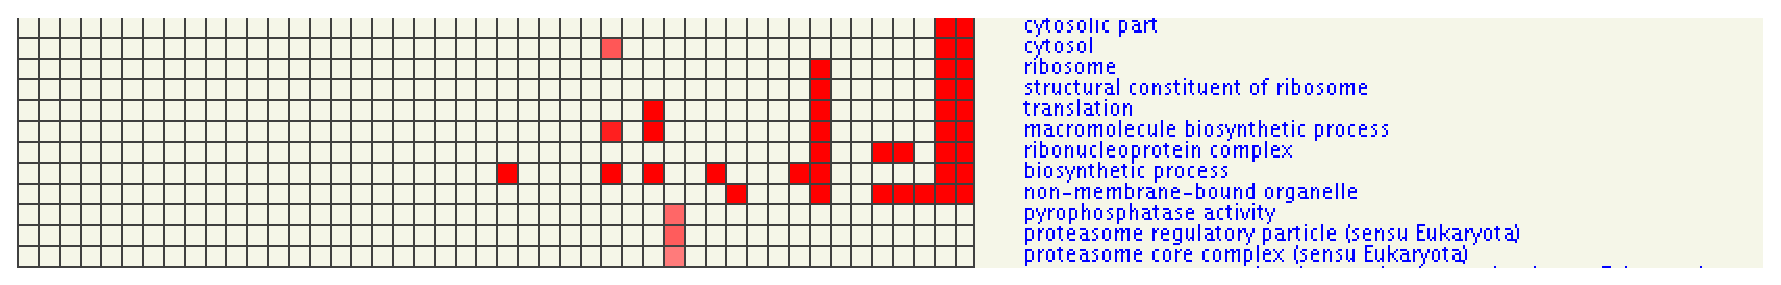
\includegraphics[scale=0.5]{images_only/semisup/results/analysis/img_stress_yt/1.eps}
\label{fig:stress_yt_enrich_1}
}
\subfigure[Section of the image showing significant enrichment]{
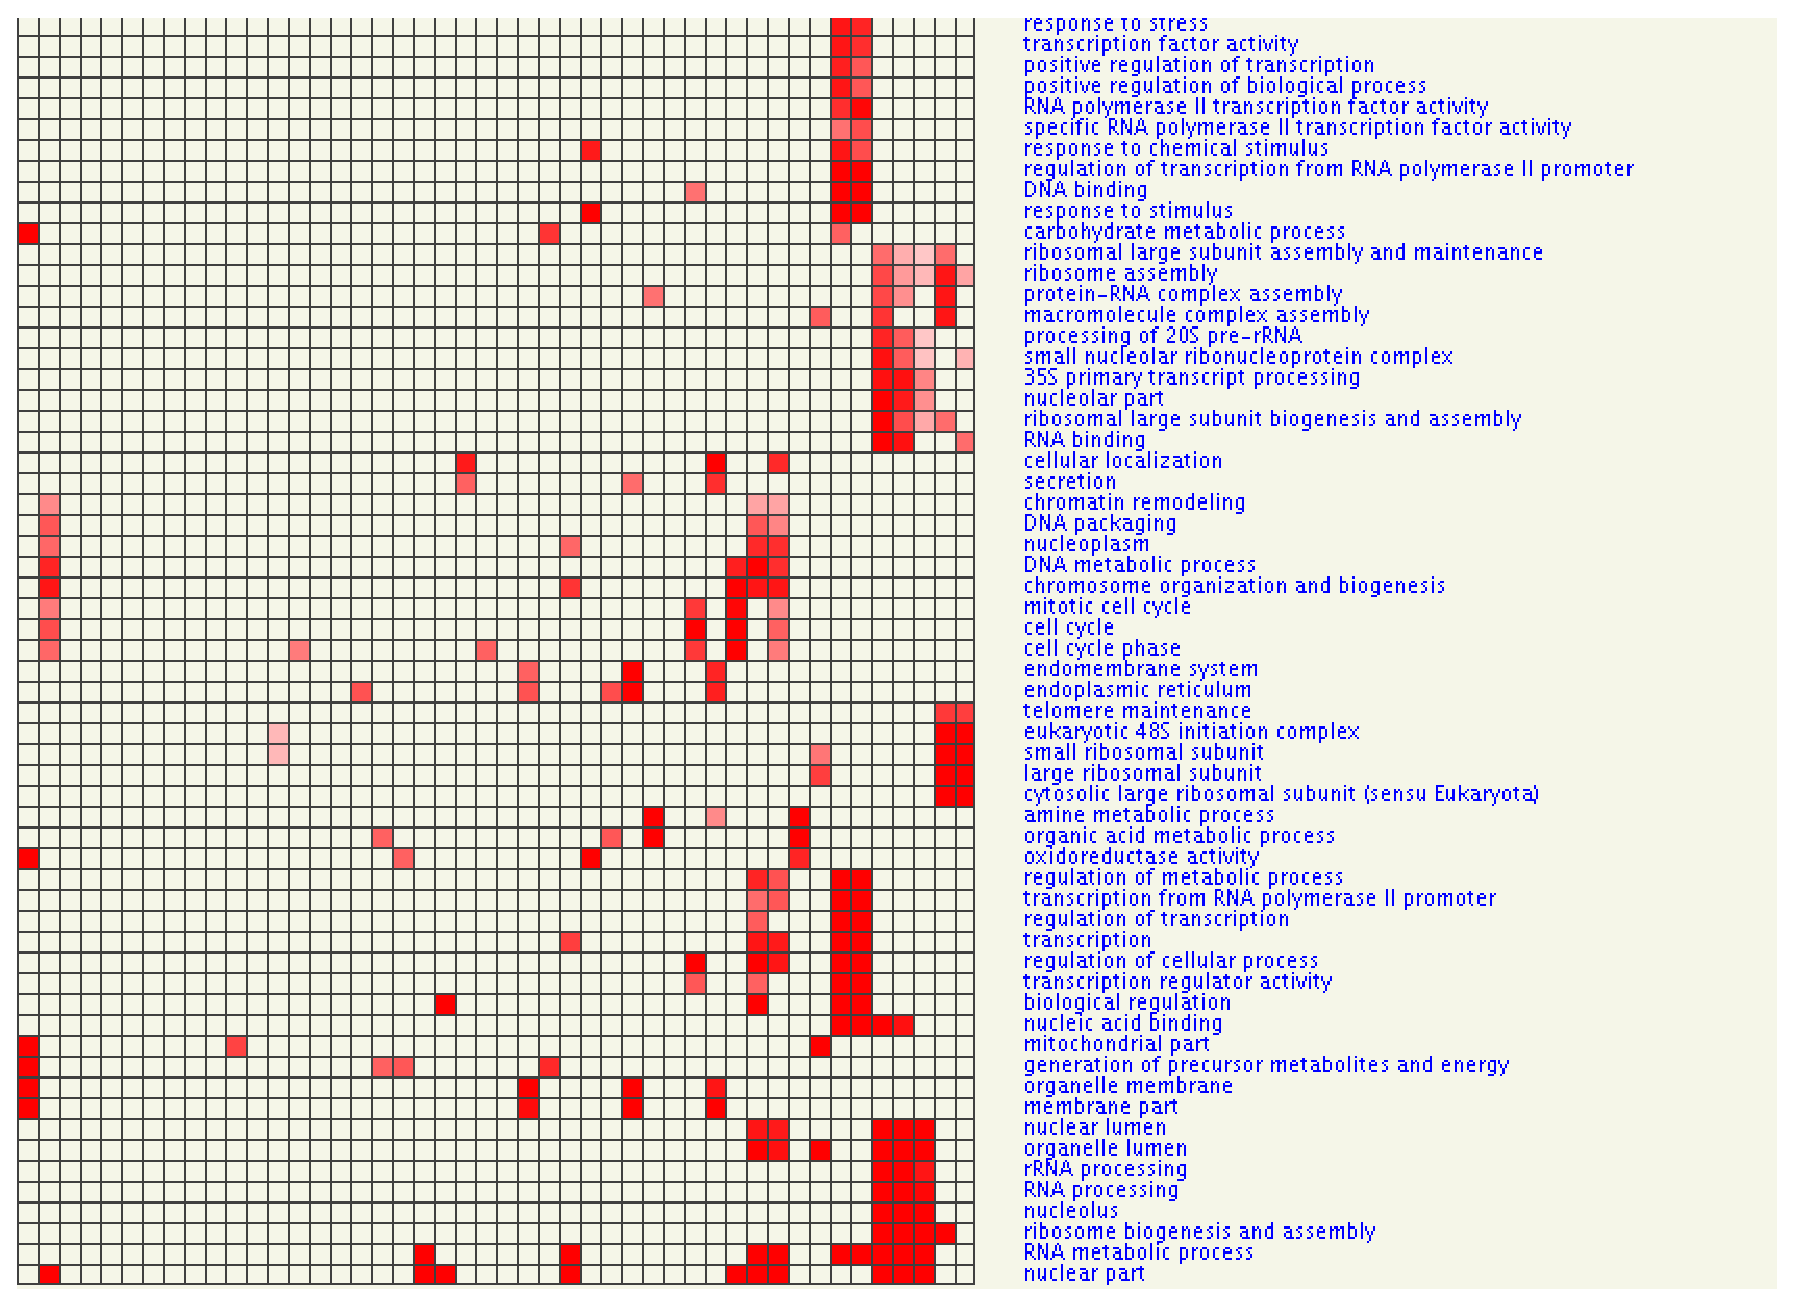
\includegraphics[scale=0.4]{images_only/semisup/results/analysis/img_stress_yt/2.eps}
\label{fig:stress_yt_enrich_2}
}
\caption{Sections of the image showing significant GO term enrichment in Stress dataset combined with knowledge (constraints) from Yeastract dataset. }
\label{fig:stress_yt_enrich}
\end{figure}

\subsubsection{Stress vs Stress and PPI}

Biological processes like RNA metabolism, RNA binding, rRNA processing, RNA processing, 35S primary transcription, nucleic acid binding, DNA metabolic process are common 
significant enrichments observed in the both the datasets. When combined with PPI dataset, it also shows significant enrichment for processes like oxidoreductase activity, 
transcription from RNA polymerase II promoter, transcription, regulation of transcription, regulation of metabolic process, developmental process, cell cycle phase, 
mitotic cell cycle, biological regulation, regulation of cellular process and chromosome organization and biogenesis when compared to Stress dataset alone. These genes associated to these
biological processes could be studied further to find relationships among them.

\subsubsection{Stress vs Stress and ChIP-chip}

Apart from processes like RNA processing, RNA metabolic process, ribosome biogenesis, macromolecule biosynthetic process and translation which are common enrichment observed 
in the two data sets, the Stress dataset when combined with ChIP-chip dataset also shows significant enrichment for processes like biosynthetic process, cellular localization, 
hydrolase activity, amine metabolic process, amine biosynthetic process, chromosome organization and biogenesis and regulation of cellular process.

\subsubsection{Stress vs Stress and Yeastract}

Translation, macromolecule biosynthetic process, biosynthetic process, 35S primary transcript processing, ribosomal biogenesis and assembly, RNA binding, DNA metabolic process, 
nucleic acid bing, rRNA processing, RNA processing and RNA metabolic process are a few of the common enriched processes observed between Stress and Stress Yeastract. 
However, processes like response to stress, transcription factor activity, positive regulation of transcription, positive regulation of biological process, 
RNA polymerase II transcription factor activity, response to chemical stimulus, regulation of transcription from RNA polymerase II promoter, 
DNA binding, response to stimulus, cellular localization, chromosome organization and biogenesis, mitotic cell cycle, cell cycle, cell cycle phase, 
telomere maintenance, amine metabolic process, organic acid metabolic process, oxidoreductase activity, regulation of metabolic process, regulation of transcription, transcription, 
regulation of cellular process, transcription of regulator activity and biological regulation are other significant enrichment observed only 
in Stress Yeastract as compared to Stress dataset.

\begin{figure}[p]
\centering
\subfigure[Section of the image showing significant enrichment]{
\includegraphics[scale=0.5]{images_only/ec2machine/semisup/results/analysis/ccycle_only/1.eps}
\label{fig:ccycle_only_enrich_1}
}
\caption{Sections of the image showing significant GO term enrichment in Cell-cycle only dataset. }
\label{fig:ccycle_only_enrich}
\end{figure}

\begin{figure}[p]
\centering
\subfigure[Section of the image showing significant enrichment]{
\includegraphics[scale=0.5]{images_only/ec2machine/semisup/results/analysis/ccycle_chip/1.eps}
\label{fig:ccycle_chip_enrich_1}
}
\subfigure[Section of the image showing significant enrichment]{
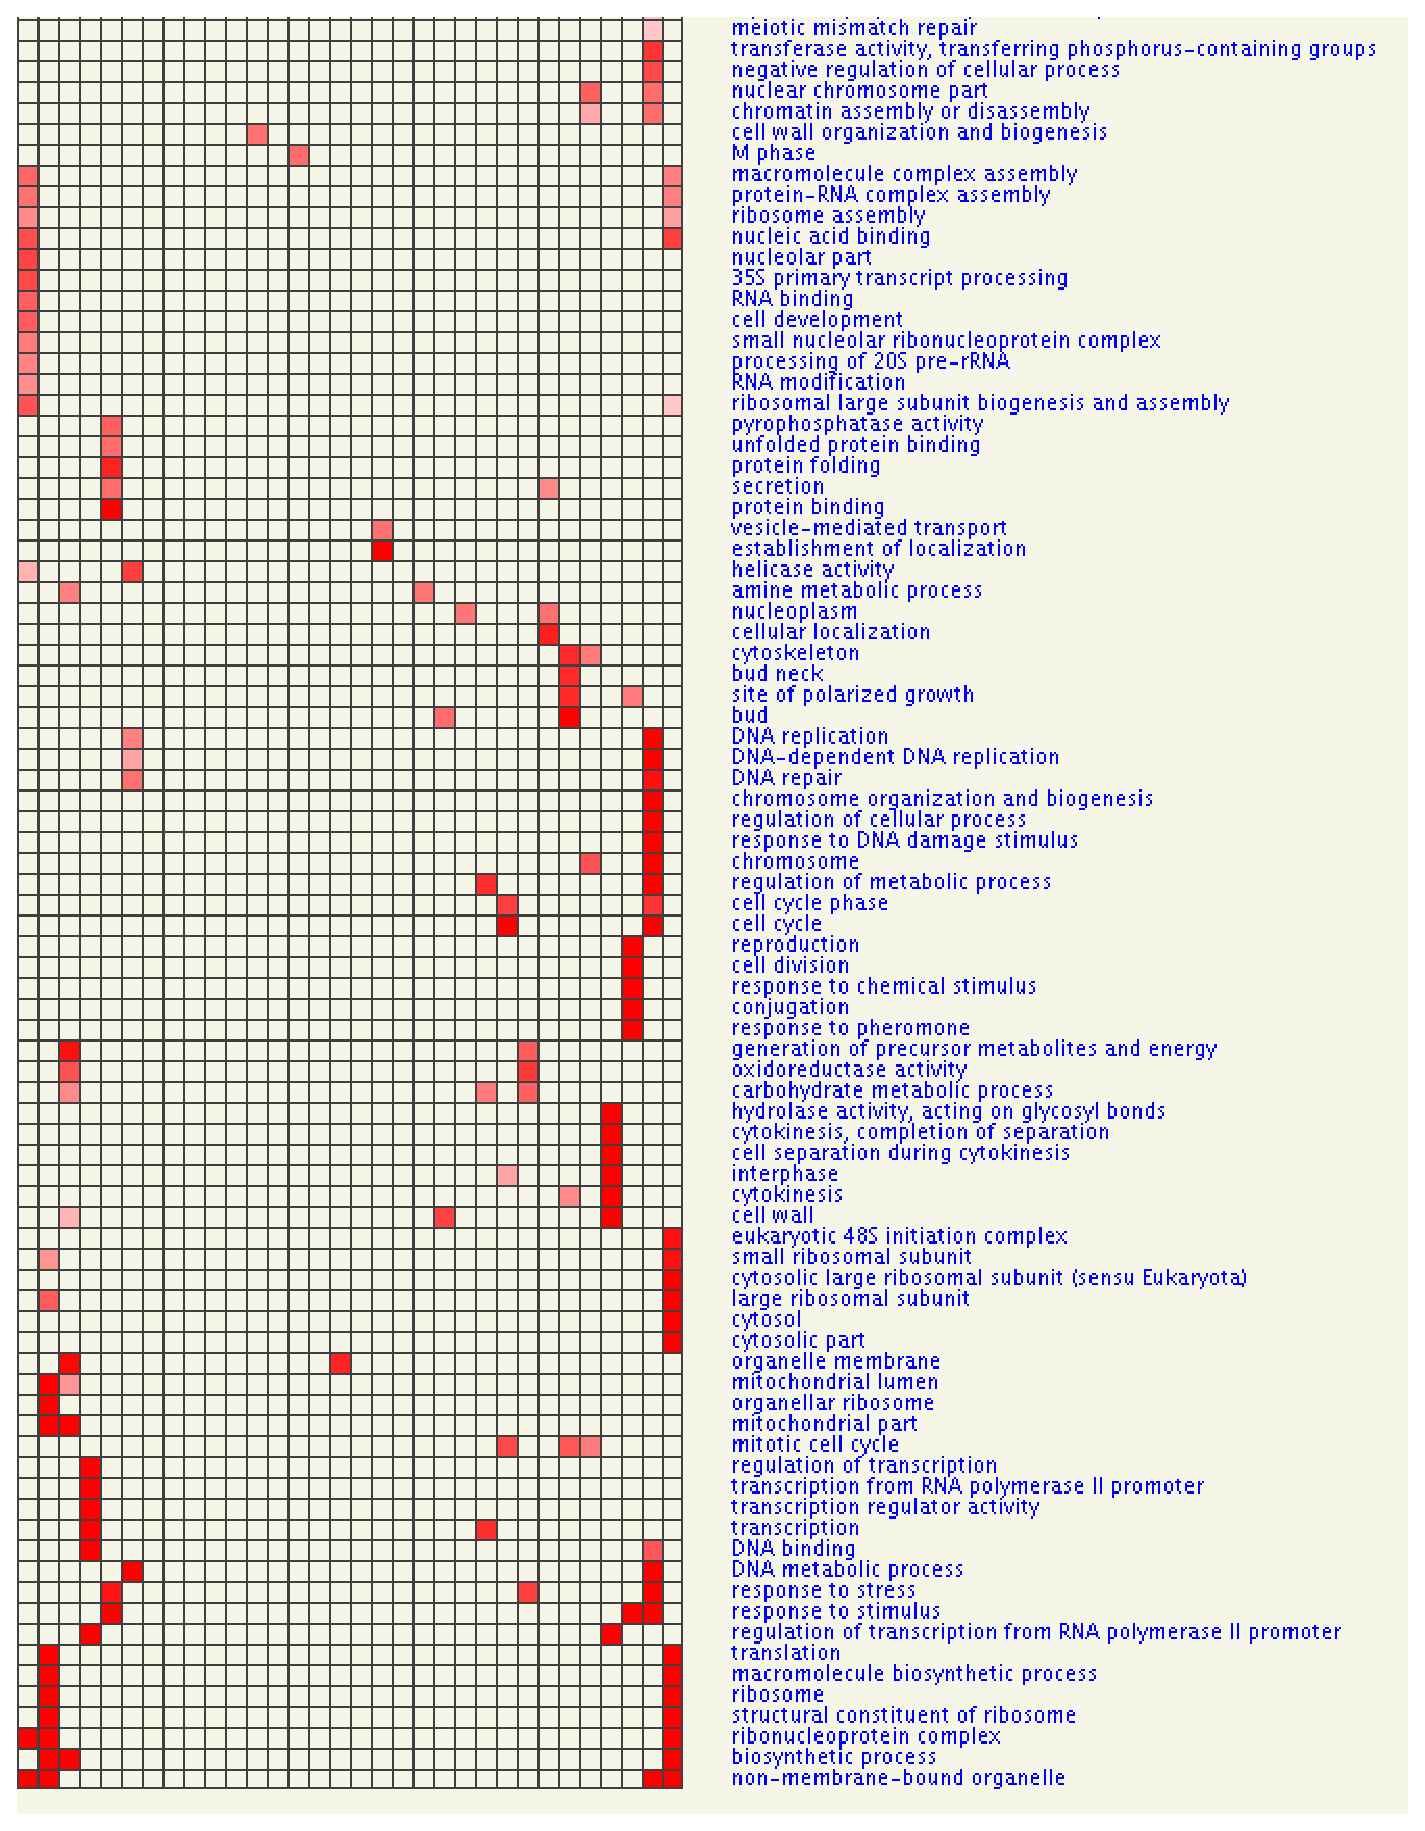
\includegraphics[scale=0.5]{images_only/ec2machine/semisup/results/analysis/ccycle_chip/2.eps}
\label{fig:ccycle_chip_enrich_2}
}
\caption{Sections of the image showing significant GO term enrichment in Cell-cycle dataset combined with knowledge (constraints) from ChIP-chip dataset. }
\label{fig:ccycle_chip_enrich}
\end{figure}

\begin{figure}[p]
\centering
\subfigure[Section of the image showing significant enrichment]{
\includegraphics[scale=0.5]{images_only/ec2machine/semisup/results/analysis/ccycle_ppi/1.eps}
\label{fig:ccycle_ppi_enrich_1}
}
\subfigure[Section of the image showing significant enrichment]{
\includegraphics[scale=0.5]{images_only/ec2machine/semisup/results/analysis/ccycle_ppi/2.eps}
\label{fig:ccycle_ppi_enrich_2}
}
\caption{Sections of the image showing significant GO term enrichment in Cell-cycle dataset combined with knowledge (constraints) from PPI dataset. }
\label{fig:ccycle_ppi_enrich}
\end{figure}

\begin{figure}[p]
\centering
\subfigure[Section of the image showing significant enrichment]{
\includegraphics[scale=0.5]{images_only/ec2machine/semisup/results/analysis/ccycle_only/1.eps}
\label{fig:ccycle_yt_enrich_1}
}

\caption{Sections of the image showing significant GO term enrichment in Cell-cycle dataset combined with knowledge (constraints) from Yeastract dataset. }
\label{fig:ccycle_yt_enrich}
\end{figure}

\subsubsection{Cell-Cycle vs Cell-Cycle and ChIP-chip}

DNA metabolic process, translation, macromolecule biosynthetic process and biosynthetic process are found to be common to the Cell-Cycle dataset before and after combination with the 
ChIP-chip dataset. After combination we see significant enrichment for response to stress, response to stimulus and regulation of transcription from polymerase II when compared 
to Cell-Cycle data set alone.

\subsubsection{Cell-Cycle Vs Cell-Cycle and PPI}

The DNA metabolic process, RNA processing, rRNA processing, the RNA metabolic process, macromolecule biosynthetic process, biosynthetic process and translation are 
some of the common enriched processes observed in both the data sets. Besides these, Cell-Cycle when combined with the PPI dataset also showed significant enrichment for 
oxidoreuctase activity, response to stress, cell-cycle, chromosome organization and biogenesis and protein binding 
when compared to the Cell Cycle data set alone. We observe that even though
cell-cycle processes were not accentuated earlier, after combination with the PPI dataset, they shows up prominently. 

\subsubsection{Cell-Cycle vs Cell-Cycle and Yeastract}

The RNA binding, 35S primary transcription process, RNA processing, rRNA processing, RNA metabolic process, macromolecule biosynthetic process, 
translation and biosynthetic process are the common significant enrichment sites observed in the Cell-Cycle dataset both before and after combination with the Yeastract dataset. 
The Cell-Cycle dataset when combined with the Yeastract dataset also showed enrichment significantly for RNA modification, response to stimulus, mitotic cell cycle 
and DNA metabolic process when compared to Cell Cycle data set alone. 

\begin{comment}
\section{Results}
\begin{table}[t]
\centering
\scalebox{0.9}{
\begin{tabular}{@{\extracolsep{\fill}}|p{0.75in}|p{0.90in}|p{0.70in}|p{0.70in}|p{0.65in}|p{0.70in}|p{0.70in}|p{0.65in}|}
\hline
\multicolumn{2}{|c|}{Constraint Source} & \multicolumn{6}{|c|}{Mean Enrichment}\\ \cline{1-8}
& p-value cutoffs (no. of constraints) & \multicolumn{3}{|c|}{across all terms} & \multicolumn{3}{|c|}{for top 50 terms}\\ \cline{3-8}
       & & Before integration &  After integration & Percent gain & Before integration &  After integration & Percent gain\\
\hline
\multirow{7}{*}{ChIP-chip}& & & & & & & \\ 
& 0.0001 (544)  &  8.101  &  9.029  &  11.457 & 11.057  &  12.266  &  10.938 \\ 
& 0.0005 (846)  &  8.101  &  8.923  &  10.151 & 11.057  &  13.324  &  20.500 \\ 
& 0.001 (1053)  &  8.101  &  8.404  &  3.735  & 11.057  &  12.546  &  13.465 \\ 
& 0.005 (1959)  &  8.101  &  7.617  &  -5.974 & 11.057  &  10.831  &  -2.048 \\ 
& 0.01 (2776)    &  8.101  &  8.613  &  6.323  & 11.057  &  12.206  &  10.389 \\ 
& 0.05 (7407)    &  8.101  &  7.927  &  -2.148 & 11.057  &  10.826  &  -2.088 \\ 
& 0.1 (12579)     &  8.101  &  7.692  &  -5.047 & 11.057  &  10.610  &  -4.045 \\ \hline
PPI  & All (442) &  8.101  &  7.849  &  -3.116 & 11.057  &  11.462  &  3.664  \\ \hline
Yeastract & All (8644) &  8.101  &  7.325  &  -9.579 & 11.057  &  10.695  &  -3.271 \\

\hline 
\end{tabular}
}
\caption{Stress microarray dataset: Comparison of mean p-values of enriched GO terms before and after supervision}
\label{tab:stress:semisup_mean_pvals}
\end{table}

\begin{table}[t]
\centering
\scalebox{0.9}{
\begin{tabular}{@{\extracolsep{\fill}}|p{0.75in}|p{0.94in}|p{0.70in}|p{0.70in}|p{0.65in}|p{0.70in}|p{0.70in}|p{0.65in}|}
\hline
\multicolumn{2}{|c|}{Constraint Source} & \multicolumn{6}{|c|}{Mean Enrichment}\\ \cline{1-8}
& p-value cutoffs (no. of constraints)& \multicolumn{3}{|c|}{across all terms} & \multicolumn{3}{|c|}{for top 50 terms}\\ \cline{3-8}
       & & Before integration &  After integration & Percent gain & Before integration &  After integration & Percent gain\\
\hline
\multirow{7}{*}{ChIP-chip}& & & & & & & \\ 
& 0.0001 (681) &   7.167 &   7.412 &   3.419	& 9.411 & 10.108 & 7.407 \\ 
& 0.0005 (1032) &   7.167 &   7.156 &   -0.158 & 9.411 & 9.547  & 1.442  \\
& 0.001 (1288)  &   7.167 &   7.124 &   -0.610 & 9.411 & 9.578  & 1.773  \\
& 0.005 (2442)  &   7.167 &   7.228 &   0.842	& 9.411 & 8.842  & -6.043 \\
& 0.01 (3505)   &   7.167 &   7.713 &   7.617	& 9.411 & 10.305 & 9.496  \\
& 0.05 (9713)   &   7.167 &   7.997 &   11.576 & 9.411 & 10.453 & 11.071 \\
& 0.1 (17055)    &   7.167 &   8.085 &   12.809 & 9.411 & 10.065 & 6.951  \\ \hline
PPI       & All (1129) &   7.167 &   6.784 &   -5.349 & 9.411 &   9.825  &   4.399 \\ \hline 
Yeastract & All (9717) &   7.167 &   7.392 &   3.134  & 9.411 &   10.155 &   7.910 \\
\hline 
\end{tabular}
}
\caption{Cell-cycle microarray dataset: Comparison of mean p-values of enriched GO terms before and after supervision}
\label{tab:ccycle:semisup_mean_pvals}
\end{table}
\end{comment}

\section{Related Work and Discussion}
\subsection{Constrained clustering}
The concept of applying prior knowledge in the form of constraints to clustering algorithms is not new. Initial \textit{supervised} clustering algorithms were modifications of traditional ones and ensured that the resulting clusters had to satisfy the applied constraints. One of the first papers in this area by \citet{bradley00constrained} proposed a constrained version of the famous \textit{k-means} \citep{MacQueen67kmeans} clustering algorithm by posing the problem in terms of minimum cost network flows. Their objective behind adding the constraints was to assign a certain minimum number of points to each cluster. \citet{tung2001constraint} have done a systematic study of various constrained clustering algorithms. \citet{basu2008constrained} is a recent book on constrained clustering.

\subsection{Semi-supervised clustering}
While constrained clustering algorithms work towards satisfying known constraints, other distance based clustering algorithms were developed in which the metric that a clustering algorithm uses in order to calculate distance between a pair of data-points was modified by incorporating constraints from other sources of data. These were the first \textit{semi-supervised} clustering algorithms. They did not enforce the constraints, but used the constraints to provide guidance in the cluster formation process. This is the crucial difference between a \textit{supervised} and a \textit{semi-supervised} clustering algorithm. In the former, the constraints are derived from known ground truth and have to be satisfied, whereas in the latter, the constraints are additional sources of information but are considered noisy and hence not necessarily exactly correct. This is a characteristic of the DNA-binding, PPI and TF-gene interactions data that we use for deriving our constraints, and also our justification for using the semi supervised algorithm. 

\citet{klein2002frominstance} used the concept of ``must-link'' and ``can-not link'' constraints on hierarchical agglomerative clustering \citep{jain1988algorithms}. 
They reported that it improved upon earlier constrained clustering algorithms and required a much smaller number of constraints for similar accuracy. 
According to them constraints suggest space-level generalizations beyond their instance-level assertions. In other words, if a point A is linked to another point B, 
then A should also probably be linked to points that are near B and \textit{vice-versa}. They used this idea to \textit{propagate} constraints. \citet{basu2004probabilistic} have 
proposed a probabilistic model for semi-supervised clustering based on \acp{HMRF} that provides a more principled framework for incorporating supervision. It combines the constraint based and distance based approached into a single unified model.
 
Our technique is likewise based on the concept of using the constraints obtained from one dataset in order to modify the similarity value that is obtained from another dataset. The key difference is that while all the previous work has used this principal to do clustering in some feature space, our technique uses the modified similarity values to cluster in spectral space (spectral clustering). 

\subsubsection{Spectral clustering}
The field of spectral clustering was started by \citet{donath1973lower} who came up with the idea of constructing graph partitions using the eigenvectors of an adjacency matrix. It has generated a lot of interest in recent years \citep{shi00normalized,ng2001onspectral} in clustering related research and has been applied from \textit{object retrieval} \citep{jain06spectral} to \textit{brain surface flattening} \citep{angenent99laplace}. A nice review of this subject and its relation to other related topics can be found in \citet{luxberg2006tutorial_spectral} and an upcoming\footnote{to be published in Feb 2010} book by \citet{ding2008spectral}.

As we have discussed earlier, spectral clustering works on similarity matrices. In that respect, it is similar to \textit{multi-dimensional scaling} or in general, the broader class of \textit{metric multidimensional scaling} \citep{deleeuw2005mds} algorithms which also operate on a similarity matrix and are useful for visualization of high dimensional data by mapping it to lower dimensions. The key difference between these and spectral clustering is that while they operate in the feature space, spectral clustering works in the spectral space. Spectral clustering has close relations to the field of non-linear dimensionality reduction techniques like \textit{manifold learning} \citep{saul2006smd, haifang2006manifold} and semi-supervised learning \citep{grira2005unsupsurvey}. \citet{nadler06fundamental} have discussed the fundamental limitations of spectral clustering. \citet{dhillon05unified} have shown the equivalence between kernel k-means \citep{johnshaw2004kernelmethods} and spectral clustering. This result gains importance when the similarity matrix is too large for eigen-decomposition and iterative techniques need to be used. 

Even before the recent interest in spectral clustering, a matrix formalism has been used to describe the functional states of transcriptional regulatory systems. \citet{gianchandani2006matrix} used such a model to characterise the properties of \acp{TRS} and facilitate the computation of the transcriptional state of the genome under any given environmental conditions. 

One of the first applications of spectral clustering to bioinformatics was by \citet{kluger2003spectral} who used it to simultaneously clusters genes and conditions (biclustering) for various cancer datasets. In a cancer context, the clusters correspond to genes that are markedly up or down regulated in patients with particular types of tumors. They present a number of variants of the approach, depending on whether the normalization over genes and conditions is done independently or in a coupled fashion. They analysed publicly available cancer expression data sets, and examined the degree to which the approach is able to identify clusters. They have also compared the performance against a number of reasonable benchmarks (e.g., direct application of SVD or normalized cuts to raw data). \citet{speer05spectral} used spectral clustering to cluster Gene Ontology terms to find sets of genes that might be functionally related. They used an information theoretic measure borrowed from text mining, where it had been used to calculate semantic similarities between words, to calculate the similarity values between the terms of the Gene Ontology.

\subsubsection{Semi-supervised spectral clustering}
\citet{kamvar03spectral} propose an algorithm for classification called \textit{spectral classification} which modifies the similarity matrix to 1 if the known training data 
belong to the same class and 0 otherwise. The similarity matrix is subject to eigen-decomposition and then classification is done in the spectral space. The advantage of doing this is that they can use labelled data (provides class constraints) as well as unlabelled data (similarity computation). They report better performance than the \textit{naive Bayes} classifier in classifying newsgroups. They have also proposed a constrained spectral clustering with must-link and cannot-link constraints along with an additive normalized laplacian \citep{fiedler1975property} and used it for classification. The results and the comparison with other algorithms for this is not systematic and clearly presented which makes it difficult to judge its performance. 

\citet{brian_semisupgraph2005} proposed a semi-supervised version of the kernel k-means algorithm. The difference between our formulation and theirs is that after modifying the similarity matrix we use spectral clustering while they have used kernel k-means algorithm. They argue that this might be better for larger datasets where eigenvalue computation might be computationally expensive whereas kernel k-means being a iterative algorithm, doesn't face this problem. This is true but the drawback with kernel k-means is that like k-means it can get stuck in local optima while spectral techniques always try to approximate the global optimum.

Most algorithms discussed till now rely critically on a good metric over their inputs. If a clustering algorithm fails to find clusters that are meaningful, then the recourse usually is to manually tweak the metric until sufficiently good clusters are found. \citet{xing2003metric} proposed an algorithm that, given examples of similar (and, if desired, dissimilar) pairs of points, \textit{learns} a distance metric that respects these relationships. They also demonstrate that the learned metrics can be used to significantly improve clustering performance. 

\subsection{Co-clustering}
This is a related and overlapping technique where two or more sources of data are combined. The key difference from semi-supervised or constrained clustering is that in co-clustering, one dataset is not used to guide the other. Rather, both the datasets are combined with equal or varying weights by combining their distance metrics to come up with a new one which is then used for clustering. We will see a detailed discussion and review in the next chapter.

\section{Conclusion}

We have proposed a technique to integrate diverse datasets where one is acting as a source of supervision on the clustering of the other. 
As part of this, we have investigated whether constraints are useful at all in order to retrieve the original clustering from a noisy version of the original dataset. We also investigated 
two methods for determining the best Gaussian kernel to obtain the affinity matrix from the data. Further, we have used a validation method which scores the resulting gene clusters 
by reference to a third type of data (Gene Ontology). Our results indicate that semi-supervised spectral clustering leads to improved biological significance if the datasets from 
which known facts are extracted is not widely varying from the datasets on which they are applied.  

Since our technique is quite generic, in future, our work can be extended by using other sources of prior knowledge, for example the similarity between 
the promoter sequences of genes. In the next chapter, we propose a technique where instead of creating definite constraints, we extract similarities from graphs of interactions and 
then integrate the datasets. It is based on the principle of maximizing the entropy of the resulting matrix. 

One of the shortcomings of this research is that it is known that gene regulation is a very condition specific activity and hence the expression values that 
we observe are a result of regulation happening at one particular time. However, the datasets that we have used are from different conditions. 
The microarray datasets as well as the DNA-binding, PPI and Yeastract datasets were not experimentally observed at the same time or even by the same researchers. 
This is also a fundamental limitation of the underlying experimental techniques, since microarrays themselves do not represent a single time point, 
but rather the integration of gene activity over a time period. Moreover, knowledge about gene modules is not complete and this hinders the validation process. 



\chapter{Maximum Entropy Kernel Integration for Regulatory Module Discovery} \label{chap_maxent}
% Add a section on Implementation Issues, choice of libraries, language etc
% compare normalized vs non-normalized combination of kernels
% maybe compare our own validation technique, p-value graph, pvalue avg
\begin{quote} ``But since the affairs of men rest still incertain, Let's reason with the worst that may befall.'' - \textit{William Shakespeare (Julius Caesar)}\end{quote} 
\section{Introduction}
As we saw in the previous chapters, each of the current datasets, e.g. microarrays, DNA-binding, protein-protein interaction and sequence datasets, provide a partial 
and noisy picture of cell regulation. Hence, integration among these is required in order to obtain an improved picture of the underlying process. Initial methods 
of data integration in regulatory module discovery were mostly ad-hoc approaches that used clustering with some form of prior knowledge. Later on these were 
enhanced to incorporate model based clustering methods as well. One of the major drawbacks of these techniques was that they worked well on vectorial data but as 
soon as other types of data were encountered, the principled nature of the algorithms broke down and they had to resort to ad-hoc statistical techniques for finding 
correlations in datasets.

In the previous chapter we proposed a similarity based method which is very pertinent for non-vectorial data as there are established techniques to compute similarity 
from these. We will continue using similarity based techniques in this chapter. The bigger challenge that we saw in the last chapter was that of 
\textit{ad hoc} combination of datasets. Since they are reported as p-values, the DNA-binding data could be interpreted as similarity values. 
The similarity values in the DNA-binding dataset were converted into constraints and then combined to the microarray data using \textit{ad hoc} p-value thresholds. 
In order to do the integration in a \textit{principled} manner, we needed a framework under which various types of data could be integrated and their effects analyzed. 
Various earlier researchers have used the Bayesian framework for merging data, but in our opinion it is unsuitable to cope with non-vectorial data (strings, graphs) 
in a principled manner as it was primarily developed for vectorial data. 

To summarise, the problem now is reduced to having two similarity matrices and we need some method to integrate them. A simpler approach to integrating matrices 
is the \textit{shrinkage} method. When there are two similarity matrices $K_{1} and K_{2}$, a final combination $K$ could be written as,
\begin{eqnarray}
K &=& \mu K_{1}+(1-\mu)K_{2}
\end{eqnarray}
which represents a \textit{convex combination}\footnote{A convex combination is a linear combination of where all coefficients are non-negative and sum up to 1} of $K_{1}$ and $K_{2}$ with the shrinkage parameter $\mu$ ranging between 0 and 1, and controlling what fraction of each similarity matrix contributes towards the final matrix. The \textit{shrinkage} method is named so because depending on the $\mu$, we shrink the contribution of the original evidence. For example, if we are combining microarray data with \ac{PPI} data to improve the predictions based just on microarray data, then the contribution of microarray data is being shrunk from its original contribution (which is 1). Optimum $\mu$ values can be chosen after running these various weight combinations of datasets through the Spectral clustering algorithm and then optimizing for the best cluster quality using the Dunn or Davies-Bouldin index values. While this is reasonable from a practical viewpoint, its not very principled. That motivates us towards our next step which is to use the principle of maximum entropy (Section-\ref{kern_integration}) in order to merge the similarity matrices. As we will see in following sections, this allows us to merge two datasets when there is no evidence available regarding their individual importance. For example, when we have two noisy data sources e.g. microarray and \ac{PPI}, and no other evidence regarding their individual importance, we can combine them to get better inference using the principle of maximum entropy.

As discussed in Section-\ref{kern_integration}, we need a more specialised version of the similarity matrix for maximum entropy integration. The extra requirement is that 
our similarity matrices should be positive semi-definite. There is a separate but similar branch of machine learning that operates only on such matrices and are 
known as \textit{kernel methods}. We describe them in Section-\ref{kern_methods}. Throughout this chapter, we have used similarity matrices, kernels and kernel 
matrices interchangeably to refer to \textit{positive semi-definite symmetric similarity matrices}.

\subsection{Spectral or eigen-decomposition}
Spectral or eigen decomposition of a symmetric $n \times n$ matrix $\mathbf{A}$ is represented as
\begin{displaymath}
    \mathbf{A} = \mathbf{Q} \Lambda \mathbf{Q}^{-1}  
\end{displaymath}
where $\Lambda = diag(\lambda_{i})$ is the diagonal matrix, $\lambda_{i}$'s are the eigenvalues of $\mathbf{A}$ and $\mathbf{Q}=[q_{1},\dots,q_{n}]$ is the square $n \times n$ matrix whose $i_{th}$ column is the basis eigenvector $q_{i}$ of $\mathbf{A}$.
  
A symmetric matrix $\mathbf{A}$ is said to be \textit{positive definite} if
\begin{displaymath}
    \mathbf{x}^{T}\mathbf{A}\mathbf{x} > 0 \mbox{ for all non-zero x}  
\end{displaymath}

A symmetric matrix $\mathbf{A}$ is said to be \textit{positive semi-definite} if
\begin{displaymath}
    \mathbf{x}^{T}\mathbf{A}\mathbf{x} \geq 0 \mbox{ for all non-zero x}  
\end{displaymath}
All the eigenvalues of a positive definite matrix are positive whereas the eigenvalues of a positive semi-definite matrix are non-negative.  

\section{Kernel Methods} \label{kern_methods}

\textit{Kernel methods} are algorithms that operate on a type of data representation known as a \textit{kernel} matrix. Kernel matrices provide a general framework to represent data and satisfy certain mathematical properties. A kernel matrix is defined not in terms of individual variables but in terms of pairwise similarity among all variables. So, instead of using a mapping $\phi:\mathcal{X}\rightarrow\mathcal{F}$ to represent each object $\mathbf{x}\in\mathcal{X}$ by $\phi(\mathbf{x})\in \mathcal{F}$, a real valued similarity function $k:\mathcal{X} \times\mathcal{X}\rightarrow\mathbb{R}$  is used and the dataset with n variables is represented by a n $\times$ n matrix of pairwise similarities $k_{ij}=k(\mathbf{x}_{i},\mathbf{x}_{j})$. The most significant fact regarding these methods is that once we have a kernel matrix representation of the data then the original data is not required and the methods can work on just these matrices. This is where the real beauty of these methods arise as different types of data types do not necessitate changes in the underlying algorithm. Kernel methods require that a kernel matrix is \textit{symmetric} and \textit{positive semi-definite}. This means that if $k$ is an $n \times n$ matrix of pairwise similarities then $k_{i,j}=k_{j,i}$ for $1 \leq i,j \leq n$, and $\mathbf{c}^\top k \mathbf{c} \geq 0$ for any $c \in \mathbb{R}^{n}$. This also implies that the matrix has non-negative real eigenvalues. 

Each similarity value ($k_{i,j}$) in a kernel matrix is calculated using a so called kernel function ( k(x,y) ) that acts a \textit{suitable} similarity between the variables. Hence, a real valued kernel matrix could be obtained for diverse data types (strings and graphs) as long as a similarity function can be defined over a pair. This nice property leads to complete separation of similarity function definition from the algorithms that operate on these matrices. This is specially useful in bioinformatics because of diverse types of datasets (as pointed in previous chapter) where a real valued representation of individual variables is non intuitive while a similarity score makes sense, e.g. genomic sequences. We will see different types of kernels in Section-\ref{kern_types}. 

\subsection{Various kernel or similarity functions}\label{kern_types}
We provide a short description of various possible kernels for different data types (vectors, strings and graphs) and their properties.

\subsubsection{Vector Data}
\begin{itemize}
 \item The \textit{Linear} or \textit{Dot kernel} is the simplest one.
\begin{equation}
 k_{L}(\textbf{x},\textbf{x}^{'})=\textbf{x}^{T}\textbf{x}^{'}
\end{equation} 
 \item The \textit{Polynomial kernel} is a more general case of the linear kernel
\begin{equation}
 k_{Poly}(\textbf{x},\textbf{x}^{'})=(\textbf{x}^{T}\textbf{x}^{'}+c)^d
\end{equation} 
where d is the degree of the polynomial and c is a constant. When c is non-zero then this kernel corresponds to a feature space spanned by all products of at most 2 variables i.e., ${\lbrace 1,x_{1},x_{2},x_{1}^{2},x_{1}x_{2},x_{2}^{2} \rbrace}$. When c is zero then this space is restricted to only the products of exactly 2 variables i.e., ${\lbrace x_{1}^{2},x_{1}x_{2},x_{2}^{2} \rbrace}$.
 \item The most popular and widely used kernel function used for real data is the \textit{Gaussian} or \textit{Radial Basis Function (RBF) kernel}
\begin{equation}
 k_{G}(\textbf{x},\textbf{x}^{'})=exp \left( -\frac{{\parallel \textbf{x}-\textbf{x}^{'} \parallel}^{2}}{2\sigma^{2}}\right)
\end{equation}
the width of the Gaussian being controlled using $\sigma$. This affinity function naturally encodes the local neighbourhood property and its value falls rapidly as the pairwise dissimilarity increases.
\item Another popularly used kernel is the \textit{Sigmoid kernel}

\begin{equation}
 k_{S}(\textbf{x},\textbf{x}^{'})=(k\textbf{x}^{T}\textbf{x}^{'}+\theta) 
\end{equation}
where $k>0$ and $\theta < 0$ are the \textit{gain} and \textit{threshold}. 

\end{itemize}

\subsubsection{Graph data}
A graph is informally defined as a set of \textit{nodes} connected by \textit{edges}. In bioinformatics, typical examples of a graph would be the interactions between the proteins of an organism or the interaction network representing the metabolic pathway. Other common examples of such graphs are social networks and hyperlinked internet web pages. While a graph represents \textit{local similarity} i.e., a node's direct interactions in its neighbourhood, we need a similarity function that represents \textit{global similarity} i.e., a node's interaction to every other node in the graph. The simplest measure of similarity on a graph is the shortest-path distance, but it is not positive semi-definite which is our requirement. Apart from this, this is very sensitive to insertions and deletions of edges. A more robust similarity measure is required which could perhaps average over many paths. The physical process of diffusion suggests a natural way of propagating such local information and has led to the most popular type of similarity on graphs known as the \textit{diffusion} kernel \citep{Kondor02diffusion}.

Laplacian $L$ of an \textit{undirected unweighted} graph is defined as,
\begin{eqnarray}
L_{i,j} &=& \begin{cases}
             -1 & \text{for i $\sim$ j,} \\
	     d_{i} & \text{for i=j,} \\
	     0 & \text{otherwise}
            \end{cases}
\end{eqnarray}
where $i \sim j$ implies that $i$ and $j$ are connected by an edge and $d_{i}$ is the number of edges originating from $i_{th}$ node. The kernel function on the graph can be defined using the negative of this Laplacian ($H=-L$) as
\begin{eqnarray}
K_{\beta} = e^{\beta H}= \lim_{m->\infty}\big ( \mathbf{I}+\frac{\beta H}{m}\big )^m
\end{eqnarray}
where $\beta$ is a positive constant and $\mathbf{I}$ is an identity matrix. $K_{\beta}$ represents an exponential family of similarity functions with generator $H$ and bandwidth parameter $\beta$. Using power series expansion this can be expanded to
\begin{eqnarray}
K_{\beta}=  \mathbf{I}+ \beta H +\frac{\beta ^2 H^2}{2} +\frac{\beta ^3 H^3}{3!} + \dots \label{diffusion}
\end{eqnarray}

Note that $e^{\beta H}$ yields a matrix but it is not the same as component-wise exponentiation $e^{\beta H_{ij}}$. If a matrix is diagonal then its exponential can be obtained by just exponentiating every entry on the diagonal, i.e., $e^{D}=diag(e^{d_{11}},e^{d_{22}},\dots,e^{d_{nn}})$. This is an important property that could be used for computing the exponential. If we diagonalise $H$ i.e., if $H = UDU^{-1}$ and D is diagonal, then $e^{H} = Ue^{D}U^{-1}$. Based on this, we have used the technique discussed in \citet{Moler2003Nineteen} to compute our matrix exponentials. It involves computing the normalized eigenvalues and eigenvectors of $H$.
\begin{equation}
    H = \sum_{i=1}^{n}v_{i}\lambda_{i}v_{i}^{T}
\end{equation}
which when replaced in Equation-\ref{diffusion}
\begin{equation}
   K_{\beta}=\sum_{i=1}^{n}v_{i}e^{\beta \lambda_{i}}v_{i}^{T}
\end{equation}

This similarity function is also known as the \textit{diffusion} function because its differential equation form resembles the diffusion equation of heat through continuous media in classical physics \citep{Kondor02diffusion}. The function of $\beta$ is to control the extent of diffusion similar to the $\sigma$ of the Gaussian kernel. In fact, as shown in \citet{kernel_methodsvert2004}, there is straightforward correspondence between the diffusion kernel and the Gaussian kernel. The former can be considered a discretized version of the latter. In the next section we discuss our actual technique of similarity matrix integration. 

\subsection{From similarities to a valid kernel}
Sometimes we have a well defined measure of similarity between a pair of objects, but the resulting matrix is not a valid kernel matrix according to the strict definition of positive semi-definiteness. In such cases, two methods have been proposed in the literature that may be used to convert the similarity matrix to a valid kernel. \citet{tsuda99supportasymmetric} have proposed a principled technique called \textit{empirical kernel map}. \citet{roth2002going} have proposed an ad-hoc technique of eigen-decomposition of the similarity matrix and then removal of negative eigenvalues. They have also showed that this preserves the cluster structure of the data. When we are not sure if the similarity matrix that we have obtained is a kernel matrix then one of these techniques could be used to make it a kernel matrix. 
\subsection{Kernel normalization}
In order to add kernels, we need to normalize them so that they are on the same scale. Given an unnormalized kernel matrix, K, the normalized version is
\begin{equation}
    \hat{K_{ij}} = \frac{K_{ij}}{\sqrt{K_{ii} \times K_{jj}}}
\end{equation} 
This can be easily computed if we define $A = (1/\sqrt{K_{11}}, \dots, 1/\sqrt{K_{nn}})$. Then, $\hat{K} = K \ast (AA^{T})$, where $\ast$ denotes element-wise product.
 
\section{Principle of Maximum Entropy}
\subsection{Entropy} \label{information_theory}
While the term \textit{entropy} is popularly associated with thermodynamics, the entropy which we describe here comes from \textit{information theory}. This branch of applied mathematics and electrical engineering which deals with quantification of information was introduced by Claude E. Shannon in his seminal paper \citep{sha48mathematical}. While this original paper dealt with the engineering problem of the transmission of information over a noisy channel, the scope of information theory has widened a lot and touches subjects as diverse as cryptography to neurobiology. The most fundamental result of this theory is the \textit{source coding theorem}, according to which, on average, the number of bits needed to represent the result of an uncertain event is given by its \textit{entropy}. In other words, \textit{entropy} is a measure of the uncertainty associated with a random variable. 

If a discrete random variable $X$ takes values $x_{1}, \dots, x_{n}$ then its entropy $H$ is
\begin{displaymath}
    H(X) = E(I(X))
\end{displaymath}

where E is the expected value and I(X) is the \textit{information} content or \textit{self-information} of X. Now, if $p(x_i)$ is the probability of $X$ taking value $x_{i}$ then the entropy can explicitly be written as
\begin{displaymath}
    H(X) = \sum_{i=1}^n p(x_i)I(x_i) = -\sum_{i=1}^n p(x_i) \log_b p(x_i),
\end{displaymath}

where b denotes the base of the logarithm. The unit of entropy is the \textit{bit} or \textit{nat} for bases 2 and e respectively. If any of the probabilities vanish ($p(x_i) = 0$ for any $i$, we use the fact that $\lim_{p\to0}p\log p = 0$ and hence the value for that particular $i$ is zero. 

\textit{Differential entropy} also known as continuous entropy tries to extend the idea of Shannon entropy which is restricted to random variables taking discrete values to continuous probability distributions, e.g. Gaussian distribution. Another widely used measure of entropy for the continuous case is the \textit{relative entropy} of a distribution also popularly known as the KL divergence (refer Section-\ref{kl-divergence}). We will later maximize the differential entropy associated with a 
Gaussian distribution in order to merge similarity matrices (refer Section-\ref{kern_integration}). 


\subsection{Principle of maximum entropy} \label{maxent_principle}
Before we discuss our technique in detail, here we discuss the background and philosophical underpinnings of principle of maximum entropy. While in the earlier section we made a strict distinction between entropy associated to thermodynamics and information theory, at a more philosophical level, connections can be made between these two seemingly unrelated subjects. According to E.T. Jaynes in his seminal papers \citep{jaynes57maxent, jaynes82onrationale} 
\begin{quotation}
Thermodynamics should be seen as an application of information theory and the thermodynamic entropy is interpreted as being an estimate of the amount of further Shannon information needed to define the detailed microscopic state of the system, that remains uncommunicated by a description solely in terms of the macroscopic variables of classical thermodynamics. 
\end{quotation}
He proposed correspondence between statistical mechanics and information theory and suggested that the entropy in statistical mechanics, and the information entropy in information theory, are essentially the same thing. Consequently, statistical mechanics should be seen just as a particular application of a general tool of logical inference and information theory.

Suppose some testable information about a probability distribution is known. If we consider the set of all probability distributions which encode this information then the \textit{principle of maximum entropy (MaxEnt)} states that the probability distribution which maximizes the information entropy in view of the testable information is the true probability distribution. By choosing to use the distribution with the maximum entropy allowed by our information, we are choosing the most \textit{uninformative} distribution possible. If we choose any distribution with lower entropy then that would imply that we are assuming information which we do not have. On the other hand, if we choose a distribution with a higher entropy that would violate the constraints of the information we possess. Thus the maximum entropy distribution is the only reasonable distribution. Maximum entropy principles are used to choose the smoothest distributions out of all possible distributions. 

In our context, intuitively, each similarity matrix represents a distribution and we need to merge them so that the final distribution doesn't make assumptions about the individual weights of the matrices because that information is unavailable. We allow maximum entropy for the resulting distribution implying no assumptions whatsoever. This is the only approach available to us for kernel integration in the unsupervised domain.

Information theory as shown in Section-\ref{information_theory} defines \textit{information} in terms of probability distributions thus providing us with a quantitative measure of uncertainty (entropy) or ignorance. This can be maximized to find the maximally unbiased probability distribution. 

\section{Maximum Entropy Kernel Integration} \label{kern_integration}

We assume the \textit{similarity matrix} which is a symmetric positive semi-definite matrix to be the \textit{covariance matrix} of a \textit{Gaussian} distribution. Based on the earlier justification for the maximum entropy principle, we need to combine two similarity matrices such that the resulting one has maximum entropy. 

Now, a Gaussian distribution is represented as,
\begin{equation}
p(\mathbf{x|\mu,\Sigma})=\frac{1}{(2\pi)^{n/2}\lvert\Sigma\rvert^{1/2}}\exp \big\lbrace -\frac{1}{2}(\mathbf{x-\mu})^{T}\Sigma^{-1} (\mathbf{x-\mu}) \big \rbrace
\end{equation}
where $\lvert\Sigma\rvert$ is the determinant of the covariance matrix $\Sigma$, and $\mu$ is the mean of distribution. Its differential entropy is given by \citep{brookes2005matrix},
\begin{eqnarray}
H(p(\mathbf{x})) &=& -\int_{-\infty}^{+\infty} \int_{-\infty}^{+\infty} \dots \int_{-\infty}^{+\infty}p(\mathbf{x})ln (p(\mathbf{x})) d\mathbf{x} \\
&=& \frac{1}{2}(n+n ln(2\pi)+ln|\Sigma|) \label{diff_entropy_gauss}
\end{eqnarray}
In order to maximize $H(p(\mathbf{x}))$ we can ignore the first two terms ($n$ and $n ln(2\pi)$) in maximizing equation-\ref{diff_entropy_gauss} as they are constants. So, it becomes a problem of maximizing the $ln|\Sigma|$ term. 
We know that the determinant of a symmetric matrix is equal to the the product of its eigenvalues, i.e.,
\[
|\Sigma|=\prod_{i=1}^{k}\lambda_{i}
\]
where $\lambda_{i}$ ($i=1\dots k$) are the $k$ eigenvalues of $\Sigma$. Therefore,
\begin{eqnarray}
ln|\Sigma|&=& ln\big (\prod_{i=1}^{k}\lambda_{i} \big) \\
&=& \sum_{i=1}^{k} ln (\lambda_{i}) \label{max_det}
\end{eqnarray}
Also, since logarithmic functions are monotonically increasing, so we can restate that \textit{in order to maximize the entropy of a Gaussian distribution, we need to maximize the $ln|\Sigma|$\footnote{this is also popularly known as log det maximization in optimization theory literature \citep{boyd2004convexopt}} which is equivalent to maximizing the sum of the eigenvalues of its covariance matrix}. Now assume that our covariance matrix is a combination of two covariance matrices and so can be rewritten as
\begin{eqnarray}
K &=& \sum_{i=1}^{2}\mu_{i}K_{i} \\
&=& \mu_{1}K_{1}+\mu_{2}K_{2}
\end{eqnarray}
where $\mu_{1}+\mu_{2}=1$. Now, according to spectral decomposition of a symmetric matrix,
\begin{eqnarray}
\Lambda &=& UKU^{T} \\ 
&=& U\big (\mu_{1}K_{1}+\mu_{2}K_{2} \big )U^{T} \\
&=& \mu_{1}UK_{1}U^{T}+\mu_{2}UK_{2}U^{T}  \\
&=& \mu_{1}Z_{1}+ \mu_{1}Z_{2} \label{eigv_split_1} 
\end{eqnarray}
where U is orthonormal and $\Lambda=diag[\lambda_{1},\lambda_{2},\dots,\lambda_{n}]$ is the diagonal matrix of eigenvalues. Matrices $Z_{1},Z_{2}$ are not diagonal matrices because U does not always diagonalises them. But, as U is the eigenvector matrix of the linear combination of $K_{1}$ and $K_{2}$, the off-diagonal elements of $Z_{1}$ and $Z_{2}$ cancel each other out \citep{thomaz2004covariance, carlos05maximum}. Therefore,
\begin{eqnarray}
\Lambda  &=& diag[\mu_{1}\lambda^{1}_{1},\mu_{1}\lambda^{1}_{2},\dots,\mu_{1}\lambda^{1}_{n}]+ diag[\mu_{2}\lambda^{2}_{1},\mu_{2}\lambda^{2}_{2},\dots,\mu_{2}\lambda^{2}_{n}] \label{eigv_split_2} \\
&=& diag[\mu_{1}\lambda^{1}_{1}+\mu_{2}\lambda^{2}_{1}, \mu_{1}\lambda^{1}_{2}+\mu_{2}\lambda^{2}_{2},\dots,\mu_{1}\lambda^{1}_{n}+\mu_{2}\lambda^{2}_{n}]  \\ 
%\lvert \Lambda \rvert &=& \prod_{i=1}^{n}{(\mu_{1}\lambda^{1}_{i}+\mu_{2}\lambda^{2}_{i})} \\
%ln \lvert \Lambda \rvert &=& \sum_{i=1}^{n}ln{(\mu_{1}\lambda^{1}_{i}+\mu_{2}\lambda^{2}_{i})}
\end{eqnarray}
where $\mu_{1}\lambda^{1}_{1},\mu_{1}\lambda^{1}_{2},\dots,\mu_{1}\lambda^{1}_{n}$ are the variance of $K_{1}$ spanned by the U eigenvector matrix and $\mu_{2}\lambda^{2}_{1},\mu_{2}\lambda^{2}_{2},\dots,\mu_{2}\lambda^{2}_{n}$ are the variance of $K_{2}$. In order to maximize the Eqn-\eqref{max_det}, we need to maximize the individual eigenvalues of the combined covariance matrix. So, effectively it implies that we need to maximize each of the $(\mu_{1}\lambda^{1}_{i}+\mu_{2}\lambda^{2}_{i})$ terms. As stated previously, the eigenvalues of positive semi-definite matrices are non-negative. We have used kernel functions to compute similarities, which resulted in our similarity matrices being positive semi-definite. Since this is a convex combination of two terms, and all the eigenvalues are non-negative, therefore, in order to maximize it, we just need to take the maximum out of both the terms because,
\begin{eqnarray}
(\mu_{1}\lambda^{1}_{i}+\mu_{2}\lambda^{2}_{i}) \leq \max (\lambda^{1}_{i},\lambda^{2}_{i})
\end{eqnarray} 
when both $\mu_{i},\lambda_{i}$ are positive. Therefore, the maximum entropy is obtained at either ($\mu_{1}$=0, $\mu_{2}=1)$ or ($\mu_{1}$=1, $\mu_{2}=0)$ for each eigenvalue, i.e., we do not take the combination of both the terms but only one of them which is the maximum. To summarise, our matrices are not combined using any particular values of $\mu_{1},\mu_{2}$ but by just picking the maximum of both the variances spanned by U. 

Till now we discussed the theoretical justification of the technique, next we discuss the practical aspects of its implementation.

\subsection{Algorithm}
From the discussion of the preceding section it is clear that in order to calculate $U$, we need a $K$ which is an unbiased (a=b) linear combination of two similarity matrices, i.e., has equal contribution from both the matrices. Since any unbiased combination gives the same set of eigenvectors we have chosen $a=b=1$. The final algorithm is described in Algorithm-\ref{alg:max_ent_integration}.

\begin{algorithm}[h]
\caption{Maximum Entropy Similarity matrix Integration}
\label{alg:max_ent_integration}
\begin{algorithmic}[1]
\REQUIRE Similarity Matrices ($K_{1}$ and $K_{2}$) 

\STATE Calculate the eigenvectors $U$ of matrix $K$ obtained by $K = K_{1} + K_{2}$.

\STATE Use this $U$ to calculate the variance contribution of both $K_{1}$ and $K_{2}$. These are  
\begin{eqnarray}
	diag[UK_{1}U^{T}] &=&  diag[\lambda^{1}_{1},\lambda^{1}_{2},\dots,\lambda^{1}_{n}] \label{var_contrib1} \\
	diag[UK_{2}U^{T}] &=&  diag[\lambda^{2}_{1},\lambda^{2}_{2},\dots,\lambda^{2}_{n}] \label{var_contrib2}
\end{eqnarray}

\STATE Now form the final eigenvalue matrix $Z$ by choosing the maximum eigenvalues from each diagonal matrix (\ref{var_contrib1} and \ref{var_contrib2}).
\begin{displaymath}
	Z =  diag[max(\lambda^{1}_{1},\lambda^{2}_{1}),max(\lambda^{1}_{2},\lambda^{2}_{2}),\dots,max(\lambda^{1}_{n},\lambda^{2}_{n})] 
\end{displaymath}
\STATE Finally, compute the maximum entropy matrix 
\begin{displaymath}
	K^{ME} = UZU^{T}
\end{displaymath}
\end{algorithmic}
\end{algorithm}  

The principal idea here is that we keep the dominant eigenvalues, while getting rid of the smaller, and hence unreliable ones, and replacing it with better ones from the other dataset. 
\section{Datasets and Methodology} \label{chap3:sec:materials}

We have used the same datasets that was used in the previous chapter as discussed in Section-\ref{chap2:sec:materials}. They are the yeast microarray 
datasets \citep{gasch00genomicexpn,spellman98comprehensive}, DNA-binding dataset \citep{harbison04transcriptional}, 
PPI dataset (from MIPS Comprehensive Yeast Genome Database (CYGD)) \citep{Gueldener2006MPact} and the TF-gene interactions (YEASTRACT) \citep{Teixeira06yeastract}. 

While in the previous chapter, we used full set of genes from the microarray datasets and applied available constraints on them, in this chapter we are unable to use 
the full set of genes. This is because now we are combining two matrices which must be similar in size. Therefore, We first pre-process and find common genes between 
pairs of datasets that are being combined. In the previous chapter, after removing the NORFs, the stress dataset had 6251 genes and cell-cycle dataset had 6257 genes. 
They had 156 and 60 experiment counts respectively. The counts get changed after finding common sets of genes among dataset apirs. The final number of common genes when pairing 
microarray datasets with ChIP-chip, PPI and Yeastract datasets are   
 
\begin{table}
\centering
\begin{tabular}{|c|c|}
\hline
Dataset Pair & Number of genes \\ 
\hline
Stress and ChIP-chip & 2346 \\
Stress and PPI       & 4508 \\
Stress and Yeastract  & 5654 \\
\hline 
Cell-cycle and ChIP-chip & 2346\\
Cell-cycle and PPI       & 4508\\
Cell-cycle and Yeastract  & 5654\\
\hline
\end{tabular}
\caption{Number of genes considered for individual dataset pairs}
\label{tab:no_constraints}
\end{table}

After pre-processing, for the microarray datasets, we compute the similarity matrices from both of them using parameters obtained by 
the optimization procedure in the previous chapter. For the PPI, Yeastract and ChIP-chip datasets that are in the form 
of pairwise interactions, we have used the total within-cluster sum of square distances as we did not have access to original data vectors but only 
the similarity (or adjacency graph). For these datasets, we need to do the optimization of the parameter for computing the diffusion matrix. 
As shown in Equation-\ref{diffusion} we need to find the optimum value for $\beta$. To do this, we first compute diffused matrices for a range of $\beta$ values 
and then we do spectral clustering on each of these diffused matrices to find the best parameter, which is the one that yields the best cluster quality. This 
optimization is different from the microarray dataset ones because here we don't have the original data vectors because of the nature of graphical data where only 
links are specified. Because of this, we can't use distance based optimization techniques. So we have used a simpler and straightforward metric called \textit{withinss} in order 
to judge the cluster quality. For a clustering run of the algorithm, we compute this by finding the cumulative sum across all the clusters of sum of squared 
distance of all points in a cluster from its cluster centre.
\begin{equation}
    \mathit{withinss}=\sum_{i=1}^{k}\sum_{x_{ij}\in \mathbf{C}_{i}}(x_{ij}-\bar{x}_{i})^2
\end{equation}
where $C_{1},\dots,C_{k}$ are the different clusters and $\bar{x}_{i}$ are the cluster centres. Since we do not have access to the data points, we compute the \textit{withinss} of the vectors on which k-means clustering is done for spectral clustering (refer Step-6 of Algorithm-\ref{alg:spectral_clustering}). A better clustering will have a lower $withinss$ value (hence more compact). 
 
Once we have the similarity matrices from both datasets that are being integrated, we merge both of them using the maximum entropy technique as 
discussed in Algorithm-\ref{alg:max_ent_integration}. We then use spectral clustering on resulting similarity matrix to get our final clusters and then validate 
the biological significance of our results using the Gene Ontology annotations like the previous chapter.

\subsection{Parameter optimisation results}\label{param_optimisation}

\subsubsection{Chip-Chip, PPI and Yeastract datasets}
As seen in Figure-\ref{fig:chip_withinss}, for the ChIP-chip dataset, the optimum value (smallest vwithinss value implies tightest clustering) is at $\beta=10$ where the total 
withinss falls significantly. It also has one of the smallest standard deviation at that point. For the PPI dataset, as seen in Figure-\ref{fig:ppi_withinss}, the optimum 
value again is at $\beta=10$ where it has the smallest withinss value. Even though the standard deviation is not the lowest, yet we choose is because of the smallest value.
Figure-\ref{fig:yt_withinss} for the Yeastract dataset, has a optimum range between $\beta=5$ and $\beta=10$, where the optimum value is at $\beta=5$ while the combination of small value and small standard deviation 
is at $\beta=10$. We chose $\beta=5$ because of the smallest withinss value.    

\begin{figure}[htp]
  \begin{center}
    \subfigure[ChIP-chip $\beta$ optimization using total within-cluster sum of square distances]
            {\label{fig:chip_withinss}\includegraphics[scale=0.7]{/home/alok/phd/post_viva/maxent/results/sigmaopt/plots/chip_withinss.eps}}
    \subfigure[PPI $\beta$ optimization using total within-cluster sum of square distances]
            {\label{fig:ppi_withinss}\includegraphics[scale=0.7]{/home/alok/phd/post_viva/maxent/results/sigmaopt/plots/ppi_withinss.eps}} \\
    \subfigure[Yeastract $\beta$ optimization using total within-cluster sum of square distances]
            {\label{fig:yt_withinss}\includegraphics[scale=0.7]{/home/alok/phd/post_viva/maxent/results/sigmaopt/plots/yt_withinss.eps}}
  \end{center}
  \caption{ChIP-chip, PPI and Yeastract datasets: Beta optimization}
  \label{fig:chip_ppi_yt_opt}
\end{figure}

\section{Biological Significance Analysis}

\subsection{Numerical Biological Significance comparison (using mutual information)} \label{num_biosig_mi}
\subsubsection{Results}

\begin{table}[p]
\centering
{\footnotesize
\begin{tabular}{@{\extracolsep{\fill}}|p{0.5in}|p{0.40in}|p{0.50in}|p{0.40in}|p{0.40in}|p{0.40in}||p{0.40in}|p{0.50in}|p{0.40in}|p{0.40in}|p{0.40in}|}
\hline

Datasets & & & \multicolumn{3}{|l|}{Semi-supervised integration} & \multicolumn{3}{|l|}{Maximum entropy integration}\\ \cline{2-9}
       & Dataset A &  Dataset B & After integration & Gain for A & Gain for B & After Integration & \% Gain for A & \% Gain for B\\
\hline
Stress \& ChIP-chip &  62.3   & 27.5  & 59.6  &  -4.3\%& 116.72\%   & 59.4   & -4.65\%  &  116\% \\ \hline
Stress \& PPI       &  62.3   & 29.2  & 66.5  &   6.74\%&  127.73\%  & 75.1   &  20.54\% &  157.19\% \\ \hline
Stress \& Yeastract &  62.3   & 38.0  & 94    &  50.88\%&  147.36\%  & 109.0  &  74.95\% &  186.84\% \\ \hline

\end{tabular}
}
\caption{Stress microarray dataset: Comparison of Biological significance index before and after maximum entropy data integration}
\label{tab:stress:maxent_biol_index}
\end{table}

\begin{table}[p]
\centering
{\footnotesize
\begin{tabular}{@{\extracolsep{\fill}}|p{0.5in}|p{0.40in}|p{0.50in}|p{0.40in}|p{0.40in}|p{0.40in}||p{0.40in}|p{0.50in}|p{0.40in}|p{0.40in}|p{0.40in}|}
\hline

Datasets & & & \multicolumn{3}{|l|}{Semi-supervised integration} & \multicolumn{3}{|l|}{Maximum entropy integration}\\ \cline{2-9}
       & Dataset A &  Dataset B & After integration & Gain for A & Gain for B & After Integration & Gain for A & Gain for B\\
\hline
Cell-cycle \& ChIP-chip &  39.1   & 27.5  & 39.7  &   1.53\%     &  44.36\%  & 48.2   &  23.27\% &  75.27\% \\ \hline
Cell-cycle \& PPI       &  39.1   & 29.2  & 40.9  &   4.60\%     &  40.06\%  & 39.3   &  0.51\%  &  34.58\% \\ \hline
Cell-cycle \& Yeastract &  39.1   & 38.0  & 59.3  &   51.66\%    &  35.94\%  & 47.6   & 21.73 \% &  25.26\% \\ \hline

\end{tabular}
}
\caption{Cell-cycle microarray dataset: Comparison of Biological significance index before and after maximum entropy data integration}
\label{tab:ccycle:maxent_biol_index}
\end{table}

We follow the same procedure that was followed in the previous chapter (refer Section-\ref{num_biosig_mi}) for biological validation of the resulting clusters using the technique based on 
mutual information by \citet{Gibons2002Judging}. The results of the integration of the stress microarray dataset with ChIP-chip, PPI and Yeastract are in 
Table-\ref{tab:stress:maxent_biol_index}. We have reported percentage gains in index values before and after integration for each pair of dataset being integrated. In order to compare our 
results with the semi-supervised technique, we also reran the semi-supervised experiments on the filtered (common) gene sets. For each pair of dataset, the first one is referred 
to as A and the second as B. For example, in the first full row of Table-\ref{tab:stress:maxent_biol_index}, stress dataset is referred to as A, while Chip-Chip dataset is called B. 

The results in Table-\ref{tab:stress:maxent_biol_index} clearly indicate that both our data integration techniques helps improve the quality of resulting clustering biologically. 
Both datasets A and B have improved biological significance after integration except in one scenario where Chip-Chip is integrated with Stress dataset. MaxEnt 
integration has resulted in improvements for the stress datasets with every other dataset except the Chip-Chip dataset. We also observe that the MaxEnt technique has outperformed 
the semi-supervised one except the Chip-Chip dataset combination where the semi-supervised technique shows a small improvement than the MaxEnt. 
Also, more than the stress datasets, the improvement in B datasets i.e. the Chip-Chip, PPI and Yeastract datasets, when combined, is better. 

For the cell-cycle dataset, as shown in Table-\ref{tab:ccycle:maxent_biol_index}, the results are somewhat different. Here, too both the datasets, A and B, have improved biological 
significance after integration. MaxEnt technique has resulted in improved biological significance
after combination in all the cases. However, the results for MaxEnt are not better than the semi-supervised one. While for stress dataset, the Chip-Chip dataset had performed 
better than the MaxEnt one, for the cell-cycle dataset, it's the opposite. MaxEnt is better than the semi-supervised one for the Chip-Chip dataset combination. 
For PPI and Yeastract combinations, the semi-supervised is better.
 
As we discussed earlier that this technique merges two datasets by taking their dominant eigenvectors. In the case of stress dataset, both the datasets gained biological significance whereas now cell-cycle is always the loser. The PPI, Yeastract 
are both curated datasets. Most of the curated datasets are taken from experiments that are conducted in non-stress environments to study the regular activities of genes. 
Therefore, they are more similar to the cell-cycle dataset. Because of this similarity, the cell-cycle dataset has not gained much from the others. 
In case of stress, they were very dissimilar and hence both gained information from each other which led to improvement in their scores.    

\subsection{Qualitative Biological Significance (using Gene Ontology annotations)} \label{semisup_biosig_go}

We put the final clusters of genes (before and after combination) through Genomica which is a tool to analyze the characteristics of resulting clustering using Gene Ontology and has been detailed in the 
previous chapter.
 
\begin{figure}[p]
\centering
\subfigure[Section of the image showing significant enrichment]{
\includegraphics[scale=0.5]{/home/alok/phd/post_viva/maxent/results/analysis/img_maxent_stress_chip/1.eps}
\label{fig:stress_chip_enrich_1}
}
\subfigure[Section of the image showing significant enrichment]{
\includegraphics[scale=0.4]{/home/alok/phd/post_viva/maxent/results/analysis/img_maxent_stress_chip/2.eps}
\label{fig:stress_chip_enrich_2}
}
\label{fig:stress_chip_enrich}
\caption{Sections of the image showing significant enrichment in Stress dataset combined with Chip-Chip dataset. Full image available in the Appendix}
\end{figure}

\begin{figure}[p]
\centering
\subfigure[Section of the image showing significant enrichment]{
\includegraphics[scale=0.5]{/home/alok/phd/post_viva/maxent/results/analysis/img_maxent_stress_ppi/1.eps}
\label{fig:stress_ppi_enrich_1}
}
\subfigure[Section of the image showing significant enrichment]{
\includegraphics[scale=0.4]{/home/alok/phd/post_viva/maxent/results/analysis/img_maxent_stress_ppi/2.eps}
\label{fig:stress_ppi_enrich_2}
}
\label{fig:stress_ppi_enrich}
\caption{Sections of the image showing significant enrichment in Stress dataset combined with PPI dataset. Full image available in the Appendix}
\end{figure}

\begin{figure}[p]
\centering
\subfigure[Section of the image showing significant enrichment]{
\includegraphics[scale=0.5]{/home/alok/phd/post_viva/maxent/results/analysis/img_maxent_stress_yt/1.eps}
\label{fig:stress_ppi_enrich_1}
}
\subfigure[Section of the image showing significant enrichment]{
\includegraphics[scale=0.4]{/home/alok/phd/post_viva/maxent/results/analysis/img_maxent_stress_yt/2.eps}
\label{fig:stress_ppi_enrich_2}
}
\label{fig:stress_ppi_enrich}
\caption{Sections of the image showing significant enrichment in Stress dataset combined with Yeastract dataset. Full image available in the Appendix}
\end{figure}

\subsubsection{Stress vs Stress and Chip-Chip}
Nucleic acid binding, ribosome biogenesis  and assembly, macromolecule biosynthetic process, translation and biosynthetic process are the 
few common significant enrichment observed in both the datasets. Processes like mitotic cell cycle, regulation of cell cycle, nucleotide biosynthetic process, 
ribonucleotide metabolic process, oxidoreductase activity, response to pheromone, conjugation, cell division, reproduction, organic metabolic process, 
amine metabolic process, and amine biosynthetic process were the significant enrichment sites observed in Stress Chip Chip dataset as compared to Stress.

\subsubsection{Stress vs Stress and PPI}
Protein RNA complex assembly, macromolecule complex assembly, nucleic acid binding, DNA metabolic process, rRNA processing, RNA processing, 
ribosome biogenesis and assembly and RNA metabolic process are the common enrichment. Whereas, oxidoreductase activity, carbohydrate metabolic process, 
transcription from RNA polymerase II promoter, transcription regulator activity, response to stimulus, response to stress, protein binding, mitotic cell 
cycle, cell cycle, M phase, cell cycle phase, developmental process, cell development, chromosome organization and biogenesis, biological regulation, 
regulation of cellular process and transcription are processes which were observed as highly significant enrichment in the Stress PPI dataset.

\subsubsection{Stress vs Stress and Yeastract}
Macromolecule biosynthetic process, translation. R RNA processing, RNA processing, RNA metabolic process, ribosome biogenesis and assembly, 
protein RNA complex assembly, ribosome  assembly, 35S primary transcript processing, nucleic acid binding, RNA binding, processing of 20S pre-rRNA and 
DNA metabolic process are the common enriched zones in both the sets. Processes like cellular localization, transcription, cell development, macromolecule complex 
assembly, ribosomal large subunit biogenesis and assembly, ribosomal large subunit aseembly and maintenance, sno RNA binding, carbohydrate 
metabolic process, chromosome organization and biogenesis, DNA packaging, regulation of cellular process, biological regulation, response to stimulus, 
response to stress, developmental process, amine metabolic process, generation of precursor metabolites and energy, telomere maintenance, 
oxidoreductase activity and organic acid metabolic process  are the many significant enrichment observed only in the Stress YT dataset when 
compared to Stress dataset.

\begin{figure}[p]
\centering
\subfigure[Section of the image showing significant enrichment]{
\includegraphics[scale=0.5]{/home/alok/phd/post_viva/ec2machine/maxent/results/analysis/img_maxent_ccycle_chip/1.eps}
\label{fig:ccycle_chip_enrich_1}
}
\label{fig:ccycle_chip_enrich}
\caption{Sections of the image showing significant enrichment in Cell-cycle dataset combined with Chip-Chip dataset. Full image available in the Appendix}
\end{figure}

\begin{figure}[p]
\centering
\subfigure[Section of the image showing significant enrichment]{
\includegraphics[scale=0.5]{/home/alok/phd/post_viva/ec2machine/maxent/results/analysis/img_maxent_ccycle_ppi/1.eps}
\label{fig:ccycle_ppi_enrich_1}
}
\subfigure[Section of the image showing significant enrichment]{
\includegraphics[scale=0.5]{/home/alok/phd/post_viva/ec2machine/maxent/results/analysis/img_maxent_ccycle_ppi/2.eps}
\label{fig:ccycle_ppi_enrich_2}
}
\label{fig:ccycle_ppi_enrich}
\caption{Sections of the image showing significant enrichment in Cell-cycle dataset combined with PPI dataset. Full image available in the Appendix}
\end{figure}

\begin{figure}[p]
\centering
\subfigure[Section of the image showing significant enrichment]{
\includegraphics[scale=0.5]{/home/alok/phd/post_viva/ec2machine/maxent/results/analysis/img_maxent_ccycle_yt/1.eps}
\label{fig:ccycle_yt_enrich_1}
}
\subfigure[Section of the image showing significant enrichment]{
\includegraphics[scale=0.5]{/home/alok/phd/post_viva/ec2machine/maxent/results/analysis/img_maxent_ccycle_yt/2.eps}
\label{fig:ccycle_yt_enrich_2}
}
\label{fig:ccycle_yt_enrich}
\caption{Sections of the image showing significant enrichment in Cell-cycle dataset combined with Yeastract dataset. Full image available in the Appendix}
\end{figure}



\subsubsection{Cell-Cycle vs Cell-Cycle and Chip-Chip}
Translation, macromolecule biosynthetic process and biosynthetic process are the only three common significant enrichment observed 
in both the datasets. Whereas, ribosome biogenesis and assembly, cell cycle, cell cycle phase, mitotic cell cycle, regulation of 
cell cycle, cell wall organization and biogenesis, cell wall division, reproduction, conjugation, response to pheromone, organic 
acid metabolic process, amine metabolic process and response to stimulus are the other significant enrichment 
sites observed in the Cell Cycle Chip Chip dataset.

\subsubsection{Cell-Cycle vs Cell-Cycle and PPI}
DNA metabolic process, macromolecule biosynthetic process, biosynthetic process, translation, RNA metabolic process, rRNA processing, 
RNA processing are few common enrichment in both the datasets. However, response to DNA damage stimulus, cell cycle, mitotic cell cycle, 
cell cycle phase, M phase, biological regulation, regulation of cellular process, developmental process, regulation of transcription, 
regulation of metabolic process, transcription, cellular localization, cell development, response to stimulus, response to 
stress and ribosome biogenesis assembly are processes which showed significant enrichment in the Cell Cycle PPI dataset.

\subsubsection{Cell-Cycle vs Cell-Cycle and Yeastract}
Macromolecule biosynthetic process, translation, biosynthetic process, RNA metabolic process and DNA metabolic process are common, 
whereas, response to stimulus, cell cycle, ribosome biogenesis and assembly and generation of precursor metabolites and energy are the other 
significantly enriched processes observed only in the Cell Cycle Yeastract dataset.

The goal of integration is to have more biologically relevant clusters from which hypotheses could be derived to be carried out and validated in wet labs. All our result data is available upon request. 

\section{Related Work and Discussion}

Combining evidence from multiple biological datasets is not a new phenomenon. Earlier efforts in this direction 
related to clustering were classified under co-clustering. In this technique, the datasets are combined by assigning equal 
or varying weights to each dataset. For distance based clustering techniques, individual distances derived from each datasets 
are merged in order to come up with a new one which is then used for clustering. \citet{Hanisch2002Coclustering} 
proposed a distance metric that combines information from expression data and biological networks and uses it for clustering 
genes. They define a graph distance function on a metabolic network derived from MIPS \citep{Gueldener2006MPact} 
and combine it with a correlation-based distance function for microarray gene expression measurements. They assigned 
equal weights to both the sources and then used the resulting distance for hierarchical clustering. They show that their technique was 
able to find biologically meaningful clusters. \citet{huang2006incorporating} developed a similar algorithm in which 
instead of combining the two information sources with equal weights, they used a \textit{shrinkage} approach with the 
genes belonging to the same functional classes assigned zero distance (maximal similarity) and the rest of the genes using the distance 
calculated from the microarray data. This is then used for K-medoids clustering on simulated data as well as real one for gene function 
prediction. \citet{bramier2007coclustering} proposed co-clustering based on a combined distance metric from microarray 
gene expression data and Gene Ontology terms for \ac{SOM}. Apart from distance based clustering, various researchers have combined datasets 
using model based clustering as well \citep{pan06incorporating}.

Kernel integration has been used in the field of supervised learning in order to combine kernels from different datasets. 
\citet{Holloway2006MachineLearning} used it for predicting the TF binding locations on DNA. They have used 18 different 
datasets - both sequence and non-sequence (expression, GO) and calculated kernels from them. The goal was to combine the kernels and then 
use the final combination in \ac{SVM} for classification. They have used each kernel individually and calculated the \textit{F statistic} 
(a widely used measure for performance of a classifier). In order to combine the kernels, these F values were used as weights 
for each of the kernel. One of the drawbacks is that the F-statistic does not take into account the relationship of the variables but 
only a macro view of the performace of the whole kernel encoding. They reported that combining all datasets resulted in 73\% coverage 
of known interactions. 

A more mathematically sound approach to kernel integration was developed by \citet{lanck04kerneldatafusion}. They have formulated the optimization 
problem as a convex optimization problem and then used \ac{SDP} to solve it. The technique is both statistically sound and computationally efficient. 
They used this technique in order to classify different classes of proteins (membrane vs ribosomal) using kernels derived from protein 
sequence, microarray expression and protein-protein interaction data. They have reported an improvement in the classification results when 
the kernels are combined as compared to individual kernels. The biggest drawback of such techniques is that the weights that are assigned to each 
dataset do not take into account the correlation between different variables across datasets and assigns one common weight for the 
whole dataset. Our technique tries to solve it by picking only the highest eigenvectors.

\citet{lewis06svm} did an investigation of weighted and unweighted kernel combination in classifying GO terms associated with protein 
sequences using SVM. They came to the interesting conclusion that for this particular task, unweighted combination of kernels 
is better than weighted ones. In order to compute the weights they too have used the SDP technique. \citet{Liang2008Adaptive} 
developed a technique to learn an optimal diffusion kernel as a convex combination of many kernels constructed from biological networks 
and then used the optimal kernel for protein function prediction. They report superior performance for the combined kernel 
in comparison to individual kernels. 

Most of the above kernel combination techniques are based on \textit{supervised learning} and the individual kernel weights are 
optimized using some training data. But Kernel integration in an unsupervised setting (when training data is unavailable) is hard 
because we have no way to compute the individual weights. 

\citet{Tsuda2004Learning} used a very different approach to guess a kernel matrix from incomplete data. The underlying approach is that some 
values in the matrix are known and they try to fill in the rest so that the resulting matrix has maximum possible entropy. 
They used this to compute kernels from PPI data and metabolic network and used these for the classification task and report that 
the maximum entropy kernel beats the diffusion kernel in classification accuracy. \citet{fujibuchi2007classification} have used the maximum 
entropy devised by \citet{Tsuda2004Learning} and applied it on three microarray datasets (heterogeneous kidney carcinoma, noise introduced 
leukemia and hetergenous oral cavity carcinoma metastasis) for the purpose of evaluating its classification performance as compared to 
single kernels (linear, polynomial and rbf). They report better overall performance for the maximum entropy kernel compared 
to others in classification performance.  

In practise, the principle of maximum entropy is useful when applied to verifiable information. A piece of information is verifiable if it can 
be determined whether a given distribution is consistent with it. Given this information, the maximum entropy procedure consists 
of seeking the probability distribution which maximizes information entropy, subject to the constraints of the information. This constrained 
optimization problem is typically solved using the method of Lagrange multipliers. Both these approaches to kernel approximation 
\citep{Tsuda2004Learning, fujibuchi2007classification} using maximum entropy is based on maximising the entropy subject to certain 
constraints. However, this is very different from our approach where we do not treat it as a entropy maximisation subject to certain constraints. 
We try to assume a distribution with maximum entropy as the ideal distribution when no other information is available in order to combine the 
similarity matrices. So, when we have multiple sets of evidence, e.g. PPI and microarray data, we try to combine them through their similarity 
matrices such that the resulting distribution (of the combined similarity matrix) has the maximum entropy.

The ideal scenario of its use is where one of the datasets is a very noisy sample while the other one is a \textit{compendium} or 
reference dataset collected over time from various sources. The compendium acts as an average of all known observations, which when 
combined using this technique with the sample, fills in the eigenvalues about which the sample dataset is most \textit{confused} about. 
So, the sample dataset gets to keep all its prominent eigenvalues while borrowing ones from the compendium about which it is not so confident. 


\section{Conclusion}

We have proposed a technique to integrate two diverse datasets where one is available in the form of vectorial data while the 
other is available in the form of a graph. The core idea is based on work done by \citet{thomaz2004covariance}. While they had 
used it to combine covariance matrices where one of them is singular, we have extended its use to general kernel combination after 
observing the similarities between the properties of a covariance matrix and a similarity matrix obtained using a kernel function. 

Integrating such diverse datasets is not possible unless we resort to some kind of normalization. We have used similarity functions 
to compute similarity matrices for these datasets as the \textit{normalization} step. We have used the same techniques that we used 
in the previous chapter in order to compute the similarity function parameters.
 
While in the supervised setting we have an objective function that we can use to optimize the contribution of each of 
the similarity functions, in an unsupervised setting there is no such facility. Hence, most previous works have 
used ad-hoc techniques in order to integrate different datasets. We argue that under such a setting when no further 
evidence is available to assign weights to individual datasets then the \textit{principle of maximum entropy} 
is the most natural and valid choice. Apart from conceptual elegance, other benefits of this technique are 
that no time consuming optimization is required to search for contributions of each dataset and fairly simple and 
intuitive linear algebra computations are needed. Since our technique is quite generic, in future, our work 
can be extended to integrating other sources of data, for example  the similarity between the promoter sequences of genes.  

One of the key shortcomings for the biological validation of our results is that it is not possible to get datasets 
that were generated on the same strains under similar experimental conditions. Both our datasets were compiled by 
independent researchers. When datasets that are generated under similar conditions start becoming available we 
would be more confident in assessing the biological significance of the results.

There is no gold-standard for validating the clusters and there are no reference datasets on which we can compare 
the results with other techniques. Gene ontology while being one of the more informative sources of validation is 
still an indirect validation technique. Also, there is a fundamental limitation of the underlying experimental 
techniques, since microarrays themselves do not represent a single time point, but rather the integration of 
gene activity over a time period. 

\chapter{Summary and Future Work}
\section{Summary}
The theme of this thesis is data integration. We started with outlining an empirical technique to calculate functional similarity of datasets using the concept of cluster similarity. This could be used as an index of microarray dataset similarity. We have also showed that similarity values gradually fall with increasing fraction of dissimilar data. We have established that as more diverse data-sets are merged then the similarity to individual data-sets (which have more local patterns) is reduced and the dominant ones overshadow the weaker signals. So, before taking a blind integrative approach, much care should be taken to ensure that we mix only similar types of data. We should also be careful about the choice of normalization method. In our results we demonstrated that normalization can distort the data and affect the resulting clusters significantly.

In order to integrate different types of datasets, we have proposed a technique to integrate two different types of  datasets where one is acting as a source of supervision on the clustering of the other. The source of supervision is in the form of binary constraints derived from DNA-binding, PPI and TF-gene interactions data, and are applied on microarray data. By replicating the trend available in the DNA-binding data, our results independently demonstrated that the information available in it has been successfully incorporated in the combined dataset. We computed the biological significance of the combined datasets using Gene Ontology annotations. 

Finally, we have proposed another technique to integrate two diverse datasets where one of the datasets is non-vectorial. For this, we have used the principle of maximum entropy considering it as the most valid approach under the unsupervised clustering setting where we have no other evidence regarding the weights to be assigned to individual datasets. Again, we computed the biological significance of the combined datasets using Gene Ontology annotations. 

\section{Challenges and Future Directions}
\begin{description}
\item[Holistic Data Integration] Transcriptional regulation occurs at multiple points from transcription to actual protein synthesis. It is well known that transcription activity (\ac{mRNA} concentration) alone is not a perfect indicator of protein concentration \citep{Griffin02Complementary} as there are many post translational factors, e.g. \ac{mRNA} stability, protein degradation, post-translational modifications, that affect the process. As more protein concentration data (\textit{proteome}) and newer types of data, e.g. nucleosome positions \citep{segal2007genomiccode,field2008distinct,kaplan2008nucleosome} become available, we need to develop techniques that can integrate all these and future sources of data in order to develop more precise models of regulation. Some of the ways in which our work could be extended are detailed below.
\begin{itemize}
    \item For semi-supervised clustering, our work can be extended by using other sources as prior knowledge, for example the constraints derived from known genetic interactions based on metabolic interaction data or pathway data. In future, when different types of data from experiments conducted simultaneously become available, the reliability of our technique would increase.

    \item Other sources of gene similarity could be derived from known genetic interactions based on metabolic interaction data or pathway data or similarity of promoter gene sequences \citep{jean2006kernels} and then used with the model discussed in Chapter-5.

    \item We have used the maximum entropy technique in order to combine two similarity matrices and used this integration for clustering which is known as an unsupervised classification technique in machine learning literature. We would also like to explore the possibilities of this integrated matrix which has all the properties of a \textit{kernel} to do SVM based classification and compare the results to other methods of kernel combination \citep{lanck04kerneldatafusion} and shrinkage based methods.

    \item Many researchers have used microarray data for cancer classification. Covariance matrix estimation is essential for many of these classification techniques, e.g. \ac{LDA} and \ac{RDA} as they involve computing the inverse of the covariance matrix. If the dataset has a large number of variables but only few samples, it is known as the ``Small $n$, Large $p$'' or $n\ll p$ problem. Microarray datasets are a typical case of this because the number of genes (p) is very large while the number of available microarray samples (n) is very limited. In such a case, the estimated covariance matrix looses its full rank (rank deficient). This leads to many unwanted properties. If the covariance matrix is not full rank then it is not positive definite anymore, which is a requirement for many algorithms that might use this covariance matrix as a similarity matrix, e.g. kernel based classifiers (SVM). Another bigger problem is that this rank deficient covariance matrix is not 
invertible. There has been a lot of research in proposing better estimators of the covariance matrix, e.g. \citet{schaefer05shrinkage}. As shown by \citet{carlos05maximum} where this formulation was first used for face detection, the maximum entropy principle is an ideal candidate for an estimator of the covariance matrix when some prior knowledge is available. We intend to use it for cancer classification and compare the results with existing shrinkage based methods e.g., \citet{Tai2008Incorporating}, who combined covariance matrices and then used the resulting covariance matrix in \ac{RDA} for cancer classification.  
\end{itemize}

\item[System Dynamics] Another growing area of research is based on more detailed modelling using reaction kinematics of gene products. This could help in understanding not only the qualitative models of regulation but also detailed quantitative ones. 

\item[Prior Knowledge] Most of the past research in molecular biology involved working with a small number of genes. This has led to the accumulation of a huge amount of biological knowledge. Genome wide global modelling of regulation has mostly used this high quality data for validation of the results. Apart from validation, this prior biological knowledge could be used to produce better models by integrating them along with other sources of experimental data.

\item[Incoherently Integrated Datasets] Orphanides and Reinberg (2002) argue very explicitly that there is no single model of regulation and each cell process has evolved its own detailed regulation model. Moreover, we usually observe only a few snapshots of these processes, which makes it very hard to reconstruct the underlying mechanisms. The data that is integrated comes from various laboratories where experiments are done under different conditions and with different platforms. We must be very careful while integrating such data and care must be taken to check beforehand if the data shows similar trends. The above conditions are some of the reasons why some researchers \citep{dolinski2005changing} have found the amount of overlap in the results based on different datasets to be small. 
 
\item[We Don't Know Biology fully!] Another big challenge that inhibits precise modelling of the process is lack of available data about the 3D structure of chromatin (DNA). Apart from the promoter sequence, the 3-D structure of chromatin decides whether a transcription factor is allowed access to a certain position or not. Sometimes a transcription factor itself facilitates changes in the chromatin structure that allows it access to the promoter sequence. Better techniques of modelling the chromatin structure will definitely aid in a better regulation model.

\item[Complexities of Higher Organisms] Simple unicellular organisms have the advantage that the sample of cells used in an experiment is homogeneous. Each cell is assumed to be performing the same regulatory actions. Based on the results so far, we are far away from a fully comprehensive model of regulation in even simpler organisms like yeast. Higher organisms pose other challenges because of cell and tissue heterogeneity. Apart from this, multi-cellular organisms are a big challenge as it's very difficult to segregate the expression of one cell from its neighbouring ones. Most genomic techniques measure an average signal in a sample from a cell population. When analysing a heterogeneous tissue, this is a big concern as individual signals from different cell types are obfuscated. Moreover, the averaging effect introduces an additional source of noise as the proportions of different cells are different across samples. 

\item[Validation of Results] Interpretation of results is very hard because it is done indirectly. Because of the huge quantity of hypothesis that could be derived from the clustering results, it is not possible to validate them experimentally. So most of the validation is done indirectly using other sources of data, e.g. gene ontology annotations. Even though gene ontology databases have contributed significantly to the creation of a common language to describe properties, we do not have annotations for all genes and gene products. Without high quality annotations, the best algorithms are rendered useless as we can never know how accurate they are. Another issue is that no standardised data sets exist on which existing and future techniques could be compared. Recent years have seen a huge increase in research on innovative techniques. Yet, there are no gold standards in validation unlike standardised data sets in other fields like Information Retrieval. We need more standard datasets and better validation metrics to more fruitfully analyse the effectiveness of various algorithms and measure their effectiveness progressively.
 
\end{description}

\section{Final Remarks} 

Despite all the challenges, high-throughput technologies have changed the research focus from studying a handful of genes to studying interactions at the whole genome level. The explosion in data generation has made Biology quickly move towards becoming an information science. Data integration seems to be the only approach which can help us understand the complex underlying processes responsible for functioning of organisms. Extensive amount of further research is required both in the measurement and analysis processes to improve our understanding of how genes interact. We have only begun to understand regulation quantitatively and have a long way to go before we can construct fully detailed regulatory network models. 

Future research in the area of integration will continue as more data of different types become available. The focus will likely shift towards integration of data from multiple cell types, conditions and even organisms. Apart from integration techniques, future research is likely to move towards better validation of the various techniques and the creation of gold standards against which results can be assessed. 

Despite all the challenges, positive results have been achieved with human tumour expression data while studying both individual cancers and, with an integrative approach \citep{segal04module}, simultaneously studying a large cancer compendium of multiple datasets. These have shown that the future of this area of research is bright.

\appendix
\addappheadtotoc
%\addtocontents{toc}{\protect\contentsline{chapter}{Appendix:}{}}

\chapter{GO Term Enrichment after Integration} \label{appendix:go_enrichment_results}
\centering
\small{
\begin{longtable}{|p{1in}|p{4in}|p{1in}|}
\caption[Stress microarray dataset: P-Values of enriched GO terms after supervision from ChIP-chip data]{Stress microarray dataset: P-Values of enriched Gene Ontology terms after supervision from ChIP-chip data at p-value of 0.0005} \label{appendix:semisup_stress_pval} \\

\hline \multicolumn{1}{|c|}{\textbf{Cluster Number}} & \multicolumn{1}{c|}{\textbf{Gene Ontology Term}} & \multicolumn{1}{c|}{\textbf{P-Value}} \\ \hline 
\endfirsthead

\multicolumn{3}{c}%
{{\bfseries \tablename\ \thetable{} -- continued from previous page}} \\
\hline \multicolumn{1}{|c|}{\textbf{Cluster Number}} &
\multicolumn{1}{c|}{\textbf{Gene Ontology Term}} &
\multicolumn{1}{c|}{\textbf{P-Value}} \\ \hline 
\endhead

\hline \multicolumn{3}{|r|}{{Continued on next page}} \\ \hline
\endfoot

\hline \hline
\endlastfoot

\hline
Cluster 1 & ribosome biogenesis and assembly & 6.149 \\ \hline
Cluster 1 & nucleolus & 5.354 \\ \hline
Cluster 1 & rRNA processing & 4.379 \\ \hline
Cluster 1 & RNA binding & 3.815 \\ \hline
Cluster 2 & cytosolic part & 60.129 \\ \hline
Cluster 2 & structural constituent of ribosome & 57.218 \\ \hline
Cluster 2 & cytosol & 49.521 \\ \hline
Cluster 2 & ribosome & 49.090 \\ \hline
Cluster 2 & translation & 47.320 \\ \hline
Cluster 3 & cytosolic part & 65.140 \\ \hline
Cluster 3 & structural constituent of ribosome & 61.810 \\ \hline
Cluster 3 & cytosol & 53.050 \\ \hline
Cluster 3 & ribosome & 52.559 \\ \hline
Cluster 3 & translation & 50.551 \\ \hline
Cluster 4 & ribosome & 24.158 \\ \hline
Cluster 4 & cytosolic part & 21.674 \\ \hline
Cluster 4 & translation & 19.451 \\ \hline
Cluster 4 & cytosol & 17.084 \\ \hline
Cluster 4 & structural constituent of ribosome & 15.256 \\ \hline
Cluster 5 & cell wall & 5.043 \\ \hline
Cluster 6 & oxidoreductase activity, acting on the aldehyde or oxo group of donors, NAD or NADP as acceptor & 4.567 \\ \hline
Cluster 6 & oxidoreductase activity, acting on the aldehyde or oxo group of donors & 4.216 \\ \hline
Cluster 7 & oxidoreductase activity & 4.362 \\ \hline
Cluster 8 & response to oxidative stress & 7.893 \\ \hline
Cluster 8 & oxidoreductase activity & 5.548 \\ \hline
Cluster 8 & cell redox homeostasis & 5.548 \\ \hline
Cluster 8 & peroxidase activity & 4.860 \\ \hline
Cluster 8 & organelle envelope lumen & 3.967 \\ \hline
Cluster 9 & cell redox homeostasis & 6.370 \\ \hline
Cluster 9 & peroxidase activity & 5.678 \\ \hline
Cluster 9 & oxidoreductase activity & 4.710 \\ \hline
Cluster 9 & response to oxidative stress & 3.947 \\ \hline
Cluster 10 & ribosome biogenesis and assembly & 26.783 \\ \hline
Cluster 10 & nucleolus & 21.924 \\ \hline
Cluster 10 & rRNA processing & 15.298 \\ \hline
Cluster 10 & RNA processing & 10.780 \\ \hline
Cluster 10 & ribosome assembly & 8.324 \\ \hline
Cluster 16 & regulation of transcription from RNA polymerase II promoter & 6.836 \\ \hline
Cluster 16 & transcription from RNA polymerase II promoter & 5.824 \\ \hline
Cluster 16 & transcription regulator activity & 5.701 \\ \hline
Cluster 16 & regulation of transcription & 5.471 \\ \hline
Cluster 16 & DNA binding & 5.054 \\ \hline
Cluster 17 & nucleolar part & 8.384 \\ \hline
Cluster 17 & snoRNA binding & 7.138 \\ \hline
Cluster 17 & small nucleolar ribonucleoprotein complex & 7.086 \\ \hline
Cluster 17 & nucleolus & 6.848 \\ \hline
Cluster 17 & ribosome biogenesis and assembly & 5.556 \\ \hline
Cluster 18 & amine biosynthetic process & 13.870 \\ \hline
Cluster 18 & arginine biosynthetic process & 11.668 \\ \hline
Cluster 18 & amine metabolic process & 11.155 \\ \hline
Cluster 18 & arginine metabolic process & 10.593 \\ \hline
Cluster 18 & organic acid metabolic process & 9.876 \\ \hline
Cluster 19 & ribosome biogenesis and assembly & 34.220 \\ \hline
Cluster 19 & nucleolus & 23.460 \\ \hline
Cluster 19 & rRNA processing & 14.101 \\ \hline
Cluster 19 & ribosomal large subunit biogenesis and assembly & 12.721 \\ \hline
Cluster 19 & RNA processing & 9.636 \\ \hline
Cluster 20 & carbohydrate metabolic process & 4.955 \\ \hline
Cluster 20 & energy reserve metabolic process & 4.588 \\ \hline
Cluster 20 & generation of precursor metabolites and energy & 4.057 \\ \hline
Cluster 22 & transcription regulator activity & 6.577 \\ \hline
Cluster 22 & transcription factor activity & 6.326 \\ \hline
Cluster 22 & DNA binding & 4.932 \\ \hline
Cluster 23 & carbohydrate metabolic process & 5.783 \\ \hline
Cluster 23 & energy reserve metabolic process & 4.290 \\ \hline
Cluster 25 & ribosome biogenesis and assembly & 5.439 \\ \hline
Cluster 26 & ion binding & 4.157 \\ \hline
Cluster 28 & protein folding & 15.561 \\ \hline
Cluster 28 & unfolded protein binding & 11.833 \\ \hline
Cluster 28 & protein binding & 9.214 \\ \hline
Cluster 28 & intracellular protein transport across a membrane & 6.983 \\ \hline
Cluster 28 & response to stress & 5.726 \\ \hline
Cluster 29 & aryl-alcohol dehydrogenase activity & 17.921 \\ \hline
Cluster 29 & aldehyde metabolic process & 13.764 \\ \hline
Cluster 29 & oxidoreductase activity, acting on CH-OH group of donors & 9.520 \\ \hline
Cluster 29 & oxidoreductase activity & 8.573 \\ \hline
Cluster 31 & acid phosphatase activity & 8.870 \\ \hline
Cluster 31 & periplasmic space & 5.230 \\ \hline
Cluster 31 & response to pheromone & 4.517 \\ \hline
Cluster 31 & conjugation & 3.996 \\ \hline
Cluster 32 & purine base metabolic process & 10.842 \\ \hline
Cluster 32 & nucleobase metabolic process & 9.194 \\ \hline
Cluster 32 & IMP metabolic process & 8.570 \\ \hline
Cluster 32 & aromatic compound metabolic process & 8.022 \\ \hline
Cluster 32 & nucleoside monophosphate metabolic process & 7.983 \\ \hline
Cluster 33 & siderophore transport & 11.967 \\ \hline
Cluster 33 & iron ion transporter activity & 11.171 \\ \hline
Cluster 33 & iron ion transport & 10.139 \\ \hline
Cluster 33 & siderophore-iron transport & 9.975 \\ \hline
Cluster 33 & transition metal ion transporter activity & 8.848 \\ \hline
Cluster 34 & response to inorganic substance & 5.189 \\ \hline
Cluster 35 & glutamate metabolic process & 6.397 \\ \hline
Cluster 35 & glutamine family amino acid metabolic process & 6.165 \\ \hline
Cluster 35 & tricarboxylic acid cycle intermediate metabolic process & 6.072 \\ \hline
Cluster 35 & glutamine family amino acid biosynthetic process & 5.426 \\ \hline
Cluster 35 & carbohydrate metabolic process & 4.910 \\ \hline
Cluster 37 & specific RNA polymerase II transcription factor activity & 7.123 \\ \hline
Cluster 37 & transcription regulator activity & 6.409 \\ \hline
Cluster 37 & RNA polymerase II transcription factor activity & 4.429 \\ \hline
Cluster 39 & oxidoreductase activity & 5.967 \\ \hline
Cluster 39 & glutathione peroxidase activity & 5.476 \\ \hline
Cluster 39 & pentose metabolic process & 4.567 \\ \hline
Cluster 39 & peroxidase activity & 3.886 \\ \hline
Cluster 40 & transcription from RNA polymerase II promoter & 6.783 \\ \hline
Cluster 40 & regulation of transcription from RNA polymerase II promoter & 6.724 \\ \hline
Cluster 40 & transcription regulator activity & 6.541 \\ \hline
Cluster 40 & regulation of transcription & 6.090 \\ \hline
Cluster 40 & specific RNA polymerase II transcription factor activity & 4.854 \\ \hline
Cluster 41 & ribosome biogenesis and assembly & 19.028 \\ \hline
Cluster 41 & rRNA processing & 18.252 \\ \hline
Cluster 41 & nucleolus & 16.195 \\ \hline
Cluster 41 & RNA processing & 13.336 \\ \hline
Cluster 41 & 35S primary transcript processing & 8.089 \\ \hline
Cluster 43 & nitrogen utilization & 4.386 \\ \hline
Cluster 45 & protein folding & 7.188 \\ \hline
Cluster 45 & response to stress & 6.214 \\ \hline
Cluster 45 & unfolded protein binding & 5.959 \\ \hline
Cluster 46 & ribosome biogenesis and assembly & 18.562 \\ \hline
Cluster 46 & nucleolus & 10.863 \\ \hline
Cluster 46 & rRNA processing & 7.187 \\ \hline
Cluster 46 & RNA processing & 4.478 \\ \hline
Cluster 46 & processing of 20S pre-rRNA & 4.260 \\ \hline
Cluster 49 & regulation of transcription & 5.245 \\ \hline
Cluster 49 & regulation of metabolic process & 4.967 \\ \hline
Cluster 49 & regulation of transcription from RNA polymerase II promoter & 3.827 \\ \hline

\end{longtable}
}
\newpage
\centering
\begin{longtable}{|p{1in}|p{4in}|p{1in}|}
\caption[P-Values of enriched GO terms after maximum entropy integration of stress microarray dataset and PPI dataset]{P-Values of enriched GO terms after maximum entropy integration of stress microarray dataset and PPI dataset} \label{appendix:maxent_stress_pval} \\

\hline \multicolumn{1}{|c|}{\textbf{Cluster Number}} & \multicolumn{1}{c|}{\textbf{Gene Ontology Term}} & \multicolumn{1}{c|}{\textbf{P-Value}} \\ \hline 
\endfirsthead

\multicolumn{3}{c}%
{{\bfseries \tablename\ \thetable{} -- continued from previous page}} \\
\hline \multicolumn{1}{|c|}{\textbf{Cluster Number}} &
\multicolumn{1}{c|}{\textbf{Gene Ontology Term}} &
\multicolumn{1}{c|}{\textbf{P-Value}} \\ \hline 
\endhead

\hline \multicolumn{3}{|r|}{{Continued on next page}} \\ \hline
\endfoot

\hline \hline
\endlastfoot

\hline
Cluster 8 & protein phosphatase type 1 regulator activity & 8.291 \\ \hline
Cluster 8 & phosphatase regulator activity & 7.452 \\ \hline
Cluster 9 & cytosolic part & 23.527 \\ \hline
Cluster 9 & structural constituent of ribosome & 22.340 \\ \hline
Cluster 9 & cytosol & 21.350 \\ \hline
Cluster 9 & ribosome & 18.971 \\ \hline
Cluster 9 & translation & 18.230 \\ \hline
Cluster 12 & protein folding & 15.788 \\ \hline
Cluster 12 & unfolded protein binding & 12.085 \\ \hline
Cluster 12 & protein binding & 7.431 \\ \hline
Cluster 12 & protein refolding & 6.507 \\ \hline
Cluster 12 & intracellular protein transport across a membrane & 6.215 \\ \hline
Cluster 13 & carbohydrate metabolic process & 7.394 \\ \hline
Cluster 13 & energy reserve metabolic process & 6.219 \\ \hline
Cluster 13 & generation of precursor metabolites and energy & 4.793 \\ \hline
Cluster 14 & ribosome biogenesis and assembly & 21.804 \\ \hline
Cluster 14 & nucleolus & 16.678 \\ \hline
Cluster 14 & ribosomal large subunit biogenesis and assembly & 14.446 \\ \hline
Cluster 14 & rRNA processing & 13.307 \\ \hline
Cluster 14 & RNA processing & 9.445 \\ \hline
Cluster 25 & ribosome biogenesis and assembly & 15.155 \\ \hline
Cluster 25 & nucleolus & 14.529 \\ \hline
Cluster 25 & rRNA processing & 11.664 \\ \hline
Cluster 25 & RNA processing & 8.735 \\ \hline
Cluster 25 & ribosomal large subunit biogenesis and assembly & 7.011 \\ \hline
Cluster 27 & ribosome biogenesis and assembly & 21.526 \\ \hline
Cluster 27 & nucleolus & 17.099 \\ \hline
Cluster 27 & rRNA processing & 8.120 \\ \hline
Cluster 27 & ribosome assembly & 6.172 \\ \hline
Cluster 27 & ribosomal large subunit biogenesis and assembly & 6.137 \\ \hline
Cluster 29 & sulfur amino acid metabolic process & 6.213 \\ \hline
Cluster 29 & sulfur metabolic process & 5.270 \\ \hline
Cluster 30 & autophagy & 4.588 \\ \hline
Cluster 32 & regulation of carbohydrate metabolic process & 8.660 \\ \hline
Cluster 32 & transcriptional activator activity & 7.472 \\ \hline
Cluster 32 & transcription factor complex & 5.921 \\ \hline
Cluster 32 & carbohydrate metabolic process & 5.145 \\ \hline
Cluster 32 & transcription regulator activity & 4.357 \\ \hline
Cluster 33 & ribosome biogenesis and assembly & 13.240 \\ \hline
Cluster 33 & nucleolus & 13.078 \\ \hline
Cluster 33 & rRNA processing & 8.996 \\ \hline
Cluster 33 & 35S primary transcript processing & 7.900 \\ \hline
Cluster 33 & ribosomal large subunit biogenesis and assembly & 6.616 \\ \hline
Cluster 34 & transcriptional repressor activity & 6.357 \\ \hline
Cluster 34 & chromatin assembly or disassembly & 5.151 \\ \hline
Cluster 36 & energy reserve metabolic process & 4.588 \\ \hline
Cluster 42 & cytosolic large ribosomal subunit (sensu Eukaryota) & 7.084 \\ \hline
Cluster 42 & large ribosomal subunit & 6.189 \\ \hline
Cluster 42 & ribosome & 5.567 \\ \hline
Cluster 42 & translational elongation & 5.533 \\ \hline
Cluster 42 & cytosolic part & 5.444 \\ \hline
\end{longtable}


\aloklinespacing
\addcontentsline{toc}{chapter}{Bibliography}
\bibliography{/home/alok/phd/post_viva/thesis/bioinfo} 
%\bibliography{/homes/am2203/phd/bioinfo/bioinforeports/bioinfo}
\addcontentsline{toc}{chapter}{Acronyms}
\aloklinespacing
\chapter*{Acronyms}
\begin{acronym}
\acro{mRNA}{messenger ribonucleic acid}
\acro{RNA}{ribonucleic acid}
\acro{TF}{transcription factor}
\acro{TRN}{transcriptional regulatory network}
\acro{TRS}{transcriptional regulatory system}
\acro{GRN}{gene regulatory network}
\acro{DNA}{deoxyribonucleic acid}
\acro{PPI}{protein-protein interaction}
\acro{ChIP}{chromatin immunoprecipitation}
\acro{GGM}{graphical Gaussian model}
\acro{KL}{Kullback-Leibler}
\acro{BN}{Bayesian network}
\acro{DBN}{dynamic Bayesian network}
\acro{EM}{expectation maximization}
\acro{SGD}{Saccharomyces Genome Database}
\acro{YPD}{Yeast Proteome Database}
\acro{GRAM}{Genetic Regulatory Modules}
\acro{SAMBA}{Statistical-Algorithmic Method for Bicluster Analysis}
\acro{SCPD}{\textit{Saccharomyces cerevisiae} Promoter Database}
\acro{SMD}{Stanford Microarray Database}
\acro{MAD}{median absolute deviation}
\acro{LDA}{linear discriminant analysis}
\acro{RDA}{regularized discriminant analysis}
\acro{SVM}{support vector machine}
\acro{SDP}{semi-definite programming}
\acro{SSSC}{semi-supervised spectral clustering}
\acro{KNN}{$k$-nearest neighbour}
\acro{HMRF}{Hidden Markov Random Field}
\acro{SOM}{self-organising map}
\end{acronym}

\end{document}

\begin{document}
\symbolfootnote
\bibliographystyle{apalike}
%\bibliographystyle{abbrv}

\title{\LARGE {\bf Data Integration for Regulatory Module Discovery}\\
 \vspace*{6mm}
}

\author{Alok Mishra}
\submitdate{June 2009}


\frontmatter
\maketitle
%%\preface
\begin{declaration}

I hereby declare that this submission is my own work and that, to the best of my knowledge and belief, it contains no material previously published or written by another person nor material which has been accepted for the award of any other degree or diploma of the university or other institute of higher learning, except where due acknowledgement has been made in the text.

\vspace{1in}
Name: Alok Mishra
\vspace{0.2in}

\raisebox{0.15in}{Signature:} \includegraphics[scale=0.7]{alok_sig.eps} \hspace{2.5in}  \raisebox{0.15in}{Date: 12 June 2009}

\end{declaration}



\addcontentsline{toc}{chapter}{Abstract}

\begin{abstract}

Genomic data relating to the functioning of individual genes and their products are rapidly being produced using many different and diverse experimental techniques. Each piece of data provides information on a specific aspect of the cell regulation process. Integration of these diverse types of data is essential in order to identify biologically relevant regulatory modules. In this thesis, we address this challenge by analyzing the nature of these datasets and propose new techniques of data integration.


Since microarray data is not available in quantities that are required for valid inference, many researchers have taken the blind integrative approach where data from diverse microarray experiments are merged. In order to understand the validity of this approach, we start this thesis with studying the heterogeneity of microarray datasets. We have used KL divergence between individual dataset distributions as well as an empirical technique proposed by us to calculate functional similarity between the datasets. Our results indicate that we should not use a blind integration of datasets and much care should be taken to ensure that we mix only similar types of data. We should also be careful about the choice of normalization method. 

Next, we propose a semi-supervised spectral clustering method which integrates two diverse types of data for the task of gene regulatory module discovery. The technique uses constraints derived from DNA-binding, PPI and TF-gene interactions datasets to guide the clustering (spectral) of microarray experiments. Our results on yeast stress and cell-cycle microarray data indicate that the integration is biologically meaningful. 

Finally, we propose a technique that integrates datasets under the principle of maximum entropy. We argue that this is the most valid approach in an unsupervised setting where we have no other evidence regarding the weights to be assigned to individual datasets. Our experiments with yeast microarray, PPI, DNA-binding and TF-gene interactions datasets show improved biological significance of results.

\end{abstract}



\cleardoublepage

\addcontentsline{toc}{chapter}{Acknowledgements}

\begin{acknowledgements}

First and foremost, I would like to thank my supervisor, Professor Duncan Gillies, for his support and advice over the past three years. Without his help and patience during many difficult periods, this thesis would not have been possible. Duncan is not only an excellent mentor but also a researcher in its truest meaning. I feel privileged that I had the opportunity to work with and learn from him to be humane while striving for excellence. I would also like to thank Duncan for providing me the opportunity to help three MSc students in their dissertation as well as tutorial opportunities. 

I would like to take this opportunity to thank my thesis examiners, Professor Michael Stumpf and Professor David Gilbert, for agreeing to examine my work. Also, my second supervisor, Professor Daniel Rueckert, for examining my transfer report and his valuable advice.

Imperial College and Beit Trust funded my stay for three years in this expensive city (London) with \textit{Imperial College Deputy Rector's Scholarship} and \textit{Beit Fellowship for Scientific Research}. I am thankful from the bottom of my heart for providing me this opportunity. I would also like to express my gratitude to the Department of Computing for funding my travel costs both within the United Kingdom and internationally. Many thanks to the Zebra Housing Association, for providing me a place to stay at subsidised cost, without which I would certainly have missed the joy and privilege of living in central London so close to the university. 

I would like to thank all the denizens of Room-433 of Imperial College DOC (Huxley Building) for lifelong memories. This includes non-logicians Georgia, Alexei, Joao, Peter, Simon and logicians Uri, Mohammed, Jonathan, Mark, Nick and Clemens.
	
A huge thanks to all my friends, most importantly, Lennon and Alexei for their company, support and help during various ups and downs. I would also like to thank Orlando for many a stimulating discussion and help with filling gaps in my education. 

My thanks go to the BR forum members and multitudes of other websites that provided much needed distraction when I was not working. A big thank you, to the coffee shops in and around Imperial College for the caffeine, when I was going through the daunting task of writing up this thesis.

I am grateful to my parents for their unending love, support and encouragement. Without the values that they taught me, I would not be here. I thank all my family members for encouraging me, and bearing my mood changes all along.

Finally, and most importantly, my wife Saswati, for her endless love, support and encouragement throughout this journey. It would not have been possible without you.

\end{acknowledgements}

\cleardoublepage

\begin{dedication}
  \centering \textit{To Ma, Papaji and Saswati} 
\end{dedication}

%%\input{quotes/quotes}

\body
%\normallinespacing
\mediumlinespacing
\mainmatter
\chapter{Introduction}
\begin{quote} ``We are drowning in information, while starving for wisdom'' - \textit{E.O. Wilson} \end{quote}

The most fundamental unit of life, a living cell, functions by a complex orchestration of various genes and their products (\acs{mRNA}, proteins etc.). In a more abstract manner we can say that genes are interrelated in highly structured networks of information flow in order for the cells to function. A network of such gene products (proteins) known as \acp{TF} which regulate the production of other transcription factors or other proteins is called a \acfi{TRN} or \acfi{GRN}. The understanding and reconstruction of this regulation process at a global level is one of the major challenges for the nascent field of bio-informatics \citep{kernel_methodsvert2004}. 

Considerable work has been done by molecular biologists over the past many years in identifying the functions of specific genes. In an ideal world it would be desirable to apply these results in order to build detailed models of regulation where the precise action of each gene is understood. However, the large number of genes and the complexity of the regulation process means that this approach has not been feasible. Research into discovering causal models based on the actions of individual genes has encountered a major difficulty in estimating a large number of parameters from a paucity of experimental data. Fortunately however, biological organisation opens up the possibility of modelling at a less detailed level. In nature, complex functions of living cells are carried out through the concerted activities of many genes and gene products which are organized into co-regulated sets also known as \textit{regulatory modules} \citep{segal03module}. Understanding the organization of these sets of genes will provide insights into the cellular response mechanism under various conditions. 

Recent advances in measurement technologies and computing resources have led to the wide availability of a considerable volume of genome-wide data on gene activity measured using several diverse techniques. By fusing this data using an integrative approach, we can try to unravel the regulation process at a more global level. Although an integrated model could never be as precise as one built from a small number of genes in controlled conditions, such global modelling can provide insights into higher processes where many genes are working together to achieve a task. Various techniques from statistics, machine learning \citep{hastie01statisticallearning} and computer science have been employed by researchers for the analysis and combination of the different types of data in an attempt to identify and understand the function of regulatory modules. 

There are two underlying problems resulting from the nature of the available data. Firstly, each of the different data types (microarray, DNA-binding, protein-protein interaction and sequence data) provides a partial and noisy picture of the regulatory process. They need to be integrated in order to obtain an improved and reliable picture of the whole underlying process. Secondly, the amount of data that is available from each of these techniques is severely limited. To learn good models we need lots of data \citep{yeung04fromexpr}, yet data is only available for a few experiments of each type. To alleviate this problem many researchers have taken the path of merging all available datasets before carrying out an analysis. Thus there can be some confusion regarding the term \textit{integrative} because it has been used to describe both of these two very different approaches to data integration: one among datasets of the same type, for example microarrays, but from different experiments, and the other among different types of data, for example microarray and DNA binding data. The goal of this thesis is to analyze the problems resulting from the existing integrative approaches and suggest better solutions for improved data integration.

\section{Biological Background}
This section presents a brief overview of elementary molecular biology concepts that are essential in order to fully understand this thesis. For a detailed understanding please refer to any standard text on molecular biology like \citet{alberts02molecular}\footnote{a free web book is available at \url{http://www.web-books.com/MoBio/}}; \citet{hunter_molbio93} has written a brief yet excellent introduction specially for people with computing background.

\begin{figure}
 \parbox[b]{0.5 \textwidth}{
 \begin{center}
 \scalebox{0.50}{\includegraphics{introduction/eukaryote_cell.eps}}
 \vspace{0.1in}
 \caption{\label{fig:cell}Eukaryote cell}
 \end{center}
 }
 \hfill
 \parbox[b]{0.5 \textwidth}{
 \begin{center}
 \scalebox{0.6}{\includegraphics{introduction/central_dogma.eps}}
 \vspace{0.1in}
 \caption{\label{fig:central_dogma}Central dogma of molecular biology: $DNA \longrightarrow RNA \longrightarrow Protein $}
 \end{center}
 }
 \end{figure}

Cells, which are the most fundamental units of life, differ in higher organisms, e.g. multicellular animals and plants, known as \textit{eukaryotes} from those of the less evolved \textit{prokaryotes}, e.g. bacteria, in having a well-defined \textit{nucleus} (see Figure-\ref{fig:cell}\footnote{image taken from online book at \url{http://www.estrellamountain.edu/faculty/farabee/biobk/biobooktoc.html}}) which carries the genetic material. The nucleus is the most prominent structure inside the eukaryotic cell and the genetic information inside it is contained in the form of a \ac{DNA} molecule. \ac{DNA} has a \textit{double-helix} structure formed by two complementary strands, each made up of a sequence of \textit{nucleotides} which are composed of adenine, thymine, cytosine or guanine. 

The central dogma of molecular biology is that the sequence information on the DNA is converted into \ac{RNA} through the process of \textit{transcription}. This sometimes is also referred as \textit{gene expression}. \ac{RNA}, through the process of \textit{translation} is later converted into a sequence of amino acids that results in a \textit{protein} (see Figure-\ref{fig:central_dogma}\footnote{image source: \url{http://en.wikipedia.org/wiki/File:Central\_Dogma\_of\_Molecular\_Biochemistry\_with\_Enzymes.jpg}}). The functional unit on the DNA that codes for an individual protein is known as a \textit{gene}. The sequence of the nucleotides in the double helix within a gene specifies the primary structure of a protein. The complete sequence of nucleotides on the DNA is also referred to as the \textit{DNA sequence}. 
Higher organisms are made up of various different cell types each of which performs a specific role requiring a specific set of gene products. The fascinating fact is that each of these cells contains exactly the same set of genes (DNA) but a different set of gene products. The remarkable diversity among the cells is a result of a precisely controlled mechanism of expression and regulation of a subset of genes in each cell type. 

\begin{figure}[ht]
 \centering
 \includegraphics[scale=0.6]{introduction/gene_regulation.eps}
 \caption{Gene regulation}
 \label{fig:gene_regulation}
\end{figure}
The transcription process begins when \acp{TF} are activated by a trans-membrane receptor, leading them to bind to gene regulatory elements and to promote access to the DNA and facilitate the recruitment of RNA polymerase to the transcriptional start site as shown in Figure-\ref{fig:gene_regulation}. The gene regulatory elements of the DNA, also known as \textit{promoter regions}, are situated upstream of the gene at a distance which can vary from a few base pairs to hundreds of base pairs. The regulatory elements contain binding sites for multiple transcription factors allowing each gene to respond to multiple signalling pathways and facilitate fine-tuning of the \acp{mRNA} that are produced. Once the transcription factors are bound on the regulatory elements, they can either promote or inhibit gene expression. In the case of a promoter, the process of transcription starts. A protein called RNA polymerase starts to copy the information contained in the gene into \ac{mRNA}. These \ac{mRNA} molecules, being exact replicas of the gene, contain both \textit{exons} (which will be used in the later process) and \textit{introns} (which will be removed). A process known as \textit{splicing} removes the introns and the remaining \ac{mRNA}, called spliced \ac{mRNA}, is transported out of the nucleus into the cellular material. There it is translated into a polypeptide chain with the help of ribosomes and this chain then folds into a three-dimensional structure known as protein. 

The previous paragraph gives only a partial picture. Since transcription factors themselves are proteins, the same process may regulate them. In fact, there are genes that code just for transcription factors. This process is similar to a feedback loop in which transcription factors are regulated by other transcription factors. A major goal of bioinformatics is to understand how transcription factors affect gene expression and which groups of genes are co-regulated by certain sets of transcription factors. 

\section{Data Sources}\label{bkg:datasources}
Recent technological advances have led to an explosion in both the quantity and types of data being generated. Various observation techniques capture different facets of the cell regulatory process. These are primarily generated by molecular biologists using experimental techniques. Some of the types currently available are:
\begin{itemize}
  \item \ac{mRNA} expression measured using microarrays. 
  \item Whole genome transcription factor binding measured using \ac{ChIP} on chip. 
  \item \ac{TF} binding motifs from the promoter sequences of genes. 
  \item Protein-protein interactions using co-immunoprecipitation and other techniques. 
\end{itemize}

\subsection{Microarrays}
\begin{floatingfigure}[p]{0.45\textwidth}
%\centering
\includegraphics[scale=0.25]{introduction/cdnMicroarray.eps}
\caption{A cross-section of hybridized cDNA microarray}
\label{fig:microarray}
\end{floatingfigure}

One of the most important sources of data related to the transcription process is the genome-wide measurement of \ac{mRNA} expression levels carried out using microarrays. These have received considerable attention in the last six years and various technologies for microarray measurement have been developed \citep{Schulze01navigating}. A microarray allows simultaneous measurement of the expression levels of a large number of genes. It consists of a grid of a large number of microscopic \textit{spots} of DNA oligonucleotides on a silicon chip, each containing a specific DNA sequence. Depending on the specific technique of manufacturing, these are either called \textit{cDNA microarrays} or \textit{oligonucleotide microarrays}. Microarray technology is based on the concept of \textit{hybridization} which means that DNA has complementary strands and given the right conditions, complementary strands will bind to each other. We want to measure \ac{mRNA} content, and since \ac{mRNA} is complementary to the DNA strand from which it was created, it will bind to its complement on the probe. Therefore, each of the spots contain a short section of a gene or other DNA element that we want to study as a probe to \textit{hybridize} a complementary cDNA sample (\ac{mRNA}). Before hybridization, the target is tagged with a fluorescent dye so that after hybridization, the intensity of colour detected by a fluorescence-based detector indicates the abundance of the target.

\textit{Two-channel microarrays} as shown in Figure-\ref{fig:microarray} are hybridized with samples from two conditions, e.g. diseased tissue versus healthy tissue, and are tagged with two different colours. Fluorescent dyes Cy3 (green) and Cy5 (red) are commonly used for tagging these samples. The two coloured cDNA samples are mixed and hybridized to a single microarray that is then scanned. Relative intensities of each colour are then used to identify up-regulated and down-regulated genes. On the other hand, in \textit{single-channel microarrays}, the arrays are designed to give estimates of the absolute levels of gene expression. Therefore, comparison of two conditions requires two separate single-dye hybridizations. 

Similar expression profiles identify genes that may be controlled by a shared regulatory mechanism. Paul Spellman is one of the microarray pioneers who used it to study global expression of genes at various time points in yeast cell cycle \citep{spellman98comprehensive}. He along with some other researchers \citep{gasch00genomicexpn} also studied the response of the yeast genes when subjected to various kinds of stress. Processing microarray data to reduce the errors introduced at various stages is known as \textit{normalization}. \citet{Quackenbush06computational} provides a good overview of the techniques used for normalization and analyzing while \citet{Smythe03Statistical} discuss in detail the statistical issues involved in normalization. 

\subsection{ChIP on chip}

\ac{ChIP} on chip,  also referred to as \textit{ChIP-chip} assay is a technique which allows us to study genome wide binding of transcription factors to the DNA simultaneously. It combines \textit{\ac{ChIP}} with microarray technology (chip) to determine \textit{in vivo} all the regions of interest on the DNA's promoter regions, i.e., where each of the transcription factors bind. \cite{harbison04transcriptional} determined the global genomic occupancy of 203 transcription factors in yeast, which are all known to bind to DNA in the yeast genome. \cite{lee02transcriptional} produced a similar yeast dataset for a smaller number of transcription factors. Both these researchers reported results in the form of a confidence value (statistical P value) of a transcription factor attaching to the promoter region of a gene. The reason behind using statistical techniques was to average the errors in microarray technology and account for multiple cell populations. One of the prominent problems with such approaches is that in order to infer whether a transcription factor attached to the promoter sequence or not, we have to choose an arbitrary artificial threshold of the P-value. 

\subsection{Transcription factor binding motifs}
Transcription factor binding motifs are sequence patterns observed in the intergenic regions of the genome usually located upstream of the genes (promoter region). They are thought to be responsible for allowing access of transcription factors to binding sites which eventually leads to regulation of transcription. While \textit{ChIP-chip} provides \textit{in vivo} evidence of \ac{TF} binding, this is an indirect technique that was used before the advent of \textit{ChIP-chip}. The primary reason for considering this as an information source in the presence of \textit{ChIP-chip} data is that \textit{ChIP-chip} is very noisy and uses evidence from multiple experiments \citep{lee02transcriptional} to report the possibility of a \ac{TF} binding to the promoter region of a gene in the form of a p-value. 

Most of the approaches to identifying these were based on first clustering genes by co-expression, and then looking for common sequences in the upstream regions of the genes located in the same cluster. The upstream sequences are catalogued in the \ac{YPD}, as well as \ac{SCPD} which is dedicated to the curation of yeast genes' promoter sequences \citep{zhu1999scpd}. 

\subsection{Protein-protein interactions}
\begin{floatingfigure}[p]{0.5\textwidth}
%\centering
\includegraphics[scale=1.25]{introduction/ppi.eps}
\caption{Protein-protein interactions in yeast}
\label{fig:ppi_yeast}
\end{floatingfigure}
The interactions between proteins is important for many biological functions, e.g. signal transduction, where signals from outside a cell are transmitted to the inside by protein-protein interactions of the signaling molecules. This dataset is important for our study because proteins are gene products and proteins with similar functions and localization are more likely to interact in groups. This was shown by \citet{schwikowski2000protein} where they observed that proteins of known function and cellular location tend to cluster together with 63\% of the interactions between proteins with a common functional assignment and 76\% occurring between proteins found in the same subcellular compartment. Therefore, genes producing interacting proteins are more likely to be co-regulated and have similar functionality. This was verified by \citet{ge01correlation} who provide global evidence that genes with similar expression profiles are more likely to encode interacting proteins. Protein-protein interaction data for yeast is available as a result of advances in technologies like co-immunoprecipitation, mass-spectroscopy and yeast two-hybrid assays. There has been a tremendous growth in this type of data in the recent years. \citet{Gueldener2006MPact} have manually compiled a \ac{PPI} dataset from the literature and published large-scale experiments for yeast which is used as a reference and has been called a gold standard because of its quality and comprehensiveness \citep{yu2004annotation}.
 

\section{Research Goals and Our Approach}
The underlying problem that is addressed results from the nature of the available data. The problem is two fold: firstly, each of the current datasets, e.g. microarrays, DNA-binding, protein-protein interaction and sequence datasets, provide a \textit{partial} and \textit{noisy} picture of the whole process. Hence, we need to integrate them in order to obtain an improved and reliable picture of underlying process. Secondly, the amount of data that is available for each of these types is severely limited. To \textit{learn} good models we need lots of data. Yet, data is only available for few of the experiments of one type. To alleviate this problem many researchers have taken the path of merging available datasets and then learning clusters from it. So, we see that there are two \textit{distinct} types of integration happening, one among \textit{different types} of datasets and the other among datasets of the \textit{same type} but from \textit{different experiments}.

Results are very hard to replicate when the datasets are different even if they result from experiments with the same conditions but done by different experimenters. As clearly stated by \citet{orph02thehuman} there is no single model of regulation and each cell process has evolved its own detailed regulation model. There are certain motifs that can be seen in most of the processes but the actual details of the process are very different from one another. Furthermore, for each underlying motif, the real size of the motif is very different from process to process and geneset to geneset. So, even though many researchers have used this approach of integrating data-sets (both types), its not very clear what the implications on the final results are.

The first part of our research work focuses on \textit{understanding the impact of integration} of the latter type (using datasets of the same type but different experiments) on the global modelling related to the transcriptional gene regulation processes. Most of the algorithms have justified their results \textit{qualitatively} by interpreting their results with the help of biologists. We are interested in studying the \textit{quantitative information overlap} among various datasets and whether our current algorithms are able to leverage the integration of diverse datasets in meaningful \textit{biologically relevant} results. Specifically, we studied the correlation between the theoretical distribution difference among the datasets being merged (using \ac{KL} divergence among distributions) to the functional difference among them (computed using cluster similarity). We also studied how much the functional similarity (in our case, the cluster similarity) varied because of dataset integration as we slowly integrate increasingly diverse datasets. 

The second part of our research deals with proposing a framework and analysis of integrating datasets of different types, e.g. microarray, \textit{ChIP-chip} and PPI datasets. The exact amount of overlap and correlation among functional datasets is unclear \citep{werner2002comparative,kemmeren2002protein}, yet data integration has been shown to increase the accuracy of tasks like gene function prediction compared to single source of data \citep{ge01correlation,gerstein2002proteomics}. For data integration, spectral clustering has been used as our primary tool. The main reason behind this choice is that it is based on computing similarities of variables which results in \textit{affinity} matrices. Similarity computation allows us to normalize diverse datatypes (which were previously considered unintegrable) into a common format (affinity matrices) and then integrate them. Increasingly, biological datasets are non-vectorial, e.g. sequence and PPI data (which is available as a graph). There have been a lot of recent developments in various techniques of similarity computation among these non-vectorial datasets. With this as our foundation, two innovative techniques of integrating these datasets have been proposed.

\subsection{Thesis Scope}
Bioinformatics has grown into a vast field. It is not possible to describe in detail all of the techniques that have been followed or that have been used by the providers of publicly available data. We have not included the details of \textit{within array} normalization techniques of microarray data used by their experimenters and assume that all the microarray data is suitably normalized. 

Even though we have used k-means clustering algorithm, we have not discussed it as it is one of the most well known and elementary techniques. Similarly, we have not discussed the Gene Ontology in great detail. For all these, suitable references have been provided in the thesis.
\section{Thesis Contributions and Publications}
\begin{itemize}
    \item A comprehensive and critical review of research work done in this field has been published as
	\begin{itemize}
	\item Mishra, A. and Gillies, D. (2008). Data integration for regulatory gene module discovery. In Daskalaki, A., editor, \textit{Handbook of Research on Systems Biology Applications in Medicine}. IGI Global, Hershey, PA.
        \end{itemize}	
    \item Issues related to calculation of biological significance of clusters using Gene Ontology has been published as
       \begin{itemize} 
       \item Mishra, A. and Gillies, D. (to be published in 2010). Validation Issues in Regulatory Module Discovery. In: Huma Lodhi and Stephen Muggleton (eds.), Elements of Computational Systems Biology, John Wiley \& Sons, Inc. ISBN: 0470180935.
       \end{itemize}
    \item An empirical technique to calculate the functional similarity of datasets using the concept of cluster similarity has been developed. We propose this can be used as an index for dataset similarity after showing a very high correlation with underlying data distribution differences. We have also demonstrated that dataset integration should only be done by first choosing similar datasets, otherwise the signals present in the datasets could be overwhelmed by noise. Part of this work published as
	\begin{itemize}
	    \item Mishra, A. and Gillies, D. (2007). Effect of microarray data heterogeneity on regulatory gene module discovery. \textit{BMC Systems Biology}, 1(Suppl 1):S2
	\end{itemize}
    \item A semi-supervised spectral clustering technique to integrate two datasets where one is acting as a source of supervision on the clustering of the other has been developed. We validated the results using Gene Ontology.\nocite{mishra2007data,mishra2008Semisup,mishra2007elements} Part of this work published as
	\begin{itemize}
    		\item Mishra, A. and Gillies, D. (2008). Semi supervised spectral clustering for regulatory module discovery. In \textit{Data Integration in the Life Sciences}, pages 192-203.
 	\end{itemize}
    \item A principled technique to integrate two diverse datasets where no evidence is available regarding their individual weights (importance) has been developed using the principle of maximum entropy. We validated the results after spectral clustering of the integrated matrix using Gene Ontology.
    \item Modular and reusable software implementations of all the techniques has been developed using python\footnote{a popular programming language with efficient Linear Algebra library} and R\footnote{a software environment for statistical computing}.	
\end{itemize}

\section{Thesis Outline}
The outline of this thesis is as follows. In Chapter-2, we present a critical literature review related to the evolution of the research related to transcriptional regulatory networks and modules. Even though this field is relatively new, the amount of research done is enormous because of increasing focus and funding. This chapter tries to tie together all the past efforts into a coherent story. 

In Chapter-3, we study the effect of \textit{integrating increasingly diverse microarray datasets}. For functional similarity, we compute the cluster similarity among datasets using modified Rand's index. To estimate the theoretical difference between the underlying distributions of individual datasets, we use the \ac{KL} divergence. Finally, we study the correlation between the two measures (functional and theoretical).

In Chapter-4, we start with a discussion of spectral clustering and its theoretical foundations. In order to integrate microarray datasets with other datasets e.g., PPI and DNA-binding datasets, we propose a semi-supervised spectral clustering technique. We apply this technique on two of the popular yeast microarray datasets and evaluate the results of integration using the Gene Ontology. 

While the semi-supervised algorithm is heuristic in combining separate evidence of similarity, in Chapter-5, we propose a more principled approach to integration of similarity matrices. We merge similarity matrices derived from various datasets (microarray, PPI and DNA-binding) using the principle of maximum entropy \citep{jaynes57maxent} and analyze the results.

Finally, Chapter-6 concludes this thesis with remarks about the drawbacks and challenges faced in our approach. It details where the field is heading and what would be the future challenges. We also discuss the scope and direction of extending the current work in future. 


\chapter{Regulatory Module Discovery Algorithms}
In this chapter, we review the research done in data integration techniques for regulatory module discovery. Initial research in this area involved plain clustering of microarray data. This was followed by progressively sophisticated modelling as well as integration of various data types.
   
\section{Plain Clustering} 

When microarray data started becoming available in the late 1990s, a prime goal was to identify sets of genes that act together functionally to perform certain cellular tasks such as metabolism or cell-cycle functions. In this early phase of data analysis, various clustering algorithms, e.g. \citet{eisen1998cluster}, were applied in order to find such gene modules.  An assumption behind this clustering approach was that co-expression implied co-regulation. In other words, if sets of genes were showing similar patterns of microarray expression, they must be co-regulated and hence belong to the same module. So, co-expression was assumed to imply co-regulation and co-regulation was assumed to imply similar function. However, both these assumptions are not always correct. The validity of the resulting clusters could be tested by identifying common promoter elements on the upstream portion of genes within the same cluster on the assumption that genes are co-regulated because they have similar promoter elements. Another popular way to show validity was by using gene ontology to show that the majority of genes belonging to a module were similar in function. This was done by computing the enrichment of gene ontology terms in each of the clusters. Better clusters were expected to have more significant enrichment of these terms. In these early works, no external information was used to guide the process of clustering. A review of the early techniques based on ad-hoc as well as model based clustering can be found in \citet{jong02modeling}.

\section{Causal Networks} 
Naturally, the research community wanted to model the causal relationships among various genes in much more detail, and this precipitated a second phase of modelling in which mostly Bayesian networks and their variants, such as dynamic Bayesian networks (DBNs), were applied to model the gene regulatory processes \citep{friedman00using,husmeier03sensitivity,murphy99modelling,zou05dynamic}. \citet{friedman00using} were the first to utilise Bayesian networks for modelling gene expression data and they tried two types of local distribution - discrete (multinomial) and continuous (linear Gaussian) to express the relation between dependent genes. They tested the work on the microarray expression data of \citet{spellman98comprehensive}. When networks that modelled the data accurately were identified, two pairwise features were computed from them - Markov relations and order relations. The Markov relation just checks if each gene of a pair is in the Markov blanket of the other. This would imply a direct causal relationship between them indicating a biological relation. The order relation checks if X is ancestor of Y in all the networks of an equivalence class. This can be determined directly from the directed graph by checking whether there is a path from X to Y that is directed towards Y consistently. An order relation implies that the two genes have a role in some more complex regulatory process. Temporal aspects of data were incorporated into the model by adding a discrete variable as the root. They suggested that non-linear local and temporal models should be used for better accuracy. Their analysis of the results shows that the method is sensitive to the choice of local model and in the case of the multinomial distribution is also sensitive to the discretization method used. \citet{werhli06comparative} carried out a comparative study of the performance of modelling gene regulatory networks using \acp{GGM}, relevance networks and \acp{BN}. They used both laboratory data as well as simulated data to evaluate the different approaches. They observed that on both types of data, Bayesian networks outperformed both relevance networks and graphical Gaussian models. 

The major difficulty with this fine tuned modelling approach is that for such a high dimensional problem involving many thousands of genes, the amount of experimental data available is never enough for accurate modelling. Moreover, it is very hard to deal with the cyclical feedback nature of gene networks using Bayesian networks since, without the explicit incorporation of time, they only handle acyclic relationships among the variables. The end result of such models was that the performance was not good and not many verifiable findings were made \citep{husmeier03sensitivity}. In order to improve upon the results, work was done to incorporate better prior knowledge in the Bayesian network based modelling. \citet{imoto03combining} combined PPI, DNA binding, promoter element motifs as well as literature text mining. \citet{tamada03estimating,tamada05utilizing} also used similar diverse datasets to build Bayesian network models. 

\citet{ihmels02revealing} proposed an algorithm called \textit{Signature}, which performs bi-clustering, that is to say clustering genes, and conditions together based on expression data. It is unlike the more established bi-clustering algorithms in that it does not simultaneously generate data partitions but works in steps. The input to the algorithm is a set of genes and, in the first step, experimental conditions under which these genes change their expression above a threshold are chosen. In the second stage, all genes that have changed expression significantly under these conditions are selected. They evaluate the consistency of their clustering algorithm by analysing the recurrence of the output gene sets in their resulting modules when the input is mixed with irrelevant genes. The idea is that the results of any good algorithm should not deviate too much when slight perturbations are introduced in the data. A module is considered to be reliable if it is obtained from several distinct slightly perturbed input gene sets. Since it carries out a refinement of clusters in two stages, there can be no guarantee that the results would be clustered in a globally optimal manner. A better formulation might be to use the \ac{EM} algorithm in order to maximise their objective function. 
 

\section{Supervised Module Algorithms} 

After these initial frustrations in moving from very naive modelling (plain clustering) to highly detailed modelling (\acs{DBN}), research began to tread a path somewhere in the middle. This pragmatic approach did yield very good results and is still the basis of current research. One of the most complete studies using these types of weakly supervised methods was carried out by \citet{segal03module}. Their method, called \textit{Module Networks} algorithm, takes as input a gene expression data set and a large precompiled set of candidate regulatory genes and outputs groups of co-regulated genes (modules), their regulators, and a regulation program that specifies behaviours of the modules as a function of regulator's expression and the conditions under which regulation takes place. It uses an iterative procedure that searches for a regulation program for each module (set of genes) and is based on the \ac{EM} method that is initialised with the results of another clustering algorithm. For each cluster of genes, it searches for a regulation program that provides the best prediction of the expression profiles of genes in the module as a function of the expression of a small number of genes from the regulator set. After identifying regulation programs for all clusters, the algorithm re-assigns each gene to the cluster whose program best predicts its behaviour. It iterates till convergence, refining both the regulation program and the gene partition in each iteration. 

In their experiments, they compiled a set of regulators from the \ac{SGD} \citep{cherry98sgd} and the \ac{YPD} \citep{payne98ypd} based on annotations that broadly suggest that certain genes have a regulatory role, as either a transcription factor or a signalling protein. They also identified more potential regulators by finding genes similar to those above but removing the global regulators from the list. Microarray data for gene expression for yeast was collected from the \ac{SMD}. They chose a subset that had significant gene expression change and removed from this set the cluster known to be generic environmental response genes. Finally, they added all the genes from the regulator list above. With these two datasets (expression and regulators), they use a module network learning algorithm \citep{segal05learning} to find separate sets of regulators and the regulated modules. They obtained modules that showed significant similarity in promoter element motifs as well as annotations in the gene ontology compiled by the Gene Ontology \citet{GO}. 

At about this time, more significant prior knowledge started becoming available in the form of ChIP-chip DNA binding data and other sources as described in the previous chapter. The next step of research focused on ways of integrating these datasets in order to find gene modules. 

\citet{barjoseph03computational} describe an algorithm for discovering regulatory modules. Their algorithm is called \ac{GRAM}, and combines microarray expression data with DNA-binding data. This was one of the first papers to have combined these two sources in order to achieve better clusters. DNA-binding data provides direct physical evidence of regulation and thus offers an improvement on previous work where only indirect evidence of interaction, for example promoter sequences, were used for prior information. The GRAM algorithm begins by performing an exhaustive search over all possible combinations of transcription factors indicated by the DNA-binding dataset using certain (strict) threshold P-values. This yields sets of genes that are regulated by sets of transcription factors. This gene list is filtered by studying their expression patterns to find genes that show co-expression. These act as seeds for gene modules. The next pass revisits transcription factors and expands the seed modules by adding genes with a relaxed P-value criterion that show co-expression. GRAM allows a gene to be part of more than one module. They identified 106 modules with 655 distinct genes regulated by 68 transcription factors. Within a module, the role of each transcription factor was identified as activator or repressor by analysing the correlation between the transcription factor's expression and the expression of regulated genes. Validation was done by analysing the promoter gene sequences in same cluster using the TRANSFAC \citep{transfac1996} database to identify common sequences. 

\citet{AmosTanay04revealing} analysed several diverse datasets in an attempt to reveal the modular organisation of the yeast regulation system. They defined modules as groups of genes with statistically significant correlated behaviour across the diverse datasets. Their algorithm is called \ac{SAMBA} which is an extensible framework that can be easily updated when new datasets become available. In their analysis, they have integrated expression, PPI and DNA-binding datasets. In \ac{SAMBA}, all genomic information is modelled as weighted bi-partite graphs. Nodes on one side of graph represent genes while the other side represents properties of genes, for example proteins encoded by them. Edges between property nodes and gene nodes are assigned weights. A module is a sub graph of this bi-partite graph and a high quality module is defined as a heavy sub graph in the weighted bi-partite graph. The key point is that all sources of data are considered as properties of genes or proteins encoded by genes and there is one unified representation of all data as a bi-partite graph. Since their algorithm is based on combinatorial principles rather than graph theoretic (spectral) methods, there are no guarantees of a globally optimum partitioning. For evaluation, they found the biological significance of resulting clusters by calculating the enrichment score of all gene ontology (GO) terms associated with the genes of a module and later annotated the modules with the highest valued terms, that is to say those terms that are shared by the highest number of genes. They also analysed 600 base pairs in the upstream promoter region of the genes in a module for common motif enrichment. For each potential motif, they calculated the enrichment score among all the genes of the module. The positive aspect of their approach is that it utilises all sources of information in one uniform representation and only requires a measure of similarity of genes across a subset of properties. It also allows overlapping modules (with common genes), which is not a feature of traditional clustering algorithms. One of the limitations of their approach is that all sources of data are assigned equal weights and it isn't possible to weigh them separately according to reliability or importance. 

In a later piece of work, \citet{amos05integrative} extended the work described above by investigating the \ac{SAMBA} algorithm in more detail. They analysed more diverse datasets and focused more on the biological significance of the results, explaining them much more fully. The paper mainly describes a study of fresh data in the context of an extensive compendium of existing datasets using \ac{SAMBA}. They proposed that future work should be carried out on integration across species on the basis that transcription modules are highly conserved among species. 

The work of \citet{lemmens06Inferring} is similar to other module discovery algorithms in that they propose a very simple and intuitive algorithm to find co-regulated sets of genes that have similar expression profiles, the same binding transcription factors and a commonality of promoter motifs. The principal difference from other algorithms is that where others used motif information to validate their results, they have used it in order to find the modules itself. Their algorithm, known as ReMoDiscovery works in two passes. In the first pass, known as the \textit{seed discovery} step, tightly co-expressed genes having a minimum number of common transcription factors and a minimum number of common conserved motifs are put together in separate modules known as \textit{seed modules}. In the second pass, known as the \textit{seed extension} step, the size of the modules is increased by computing the mean of the module's gene expression and ranking the remainder of the genes in the dataset in order of their decreasing correlation with the mean profile. They compared their algorithm results with \ac{SAMBA} and \ac{GRAM} (discussed earlier) and reported their findings. All parameters, such as the cut off for various datasets, have been chosen without much justification, and the basic idea seems very similar to the work of \citet{barjoseph03computational}. Some of the comparison metrics used do not seem very sound, for example average functional enrichment values have been calculated for the modules without normalising to account for the size of the modules. Similarly, summary statistics like minimum and maximum number of genes in modules do not provide relevant information for comparison of algorithms . 

\citet{huang2006incorporating} investigated a traditional clustering method known as k-medoids which is a robust version of the k-means clustering method. Unlike k-means, which uses the mean of all genes in a cluster as its centre, k-medoids uses the most central gene (median). It is found by locating the one with minimum average dissimilarity to rest of the genes. They incorporated prior knowledge into it by modifying the distance metric used while clustering. They have used microarray expression data for clustering while biological knowledge about the known similarity between pairs of genes is derived from gene ontology. Previous approaches to include biological knowledge in distance based clustering methods have used gene ontology and metabolic pathways to estimate distance or similarity measures among gene pairs and then used these along with microarray expression based distance metrics to create an average distance, which is later used to cluster expression data. Huang and Pan used a \textit{shrinkage} approach for the distance metric to shrink it towards zero in cases where there is strong evidence that two genes are functionally related. Their algorithm has two steps in which the first step uses the shrunk distance metric to cluster genes whose functionality is known from gene ontology. The second step clusters the remaining genes. In the second step clustered genes are assigned to either one of the step one clusters or to a step two cluster, depending on their distance from the medoids. The shrinkage parameter is chosen using cross validation. They evaluated their algorithm using both simulated as well as real data. In a later piece of work, \citet{pan06incorporating} used known functions of genes from existing biological research to assign different prior probabilities for a gene to belong to a cluster. He developed an \ac{EM} algorithm for this stratified mixture model. 

The research described above concerns the evaluation of individual techniques to integrate data from multiple sources. Some researchers have also focused on creating generic frameworks for data integration. \citet{Troyanskaya2003Bayesian} developed a \textit{meta} framework for integration of diverse sources of data. We call it \textit{meta} because it doesn't directly integrate the datasets but uses results from other techniques like clustering algorithms and combines them with other evidence. Their proposed framework is known as MAGIC (Multisource Association of Genes by Integration of Clusters) and is based on a Bayesian network whose conditional probability tables have been built with the advice of yeast genetic experts. Given a pair of genes, it outputs the probability that they are functionally related after weighing the evidences from various sources. Evaluation of the predictions from the system is done using gene ontology data. 

Most of the techniques that we have described work well for real (numerical) data but are less effective when dealing with string data, for example gene sequences, or graph data such as protein interactions. In many cases ad-hoc techniques have been deployed. In an approach to this problem, \citet{lanck04statframework} have proposed a framework where such diverse data could be merged in a principled manner. It is based on kernel methods \citep{johnshaw2004kernelmethods} in which algorithms work on kernel matrices that are derived from pairwise similarity among variables using kernel functions. If a valid kernel function can be defined to encode the similarity between two variables, then the methods are applicable regardless of the different types of data - strings, vectorial or graphical - being used. This framework provides a means to integrate more diverse types of data as and when they become available in the future. The original paper proposed the framework only for supervised learning but extensions to unsupervised learning are possible. 



\chapter{Data Integration for Regulatory Module Discovery}
\section{Introduction}

As discussed in the first chapter, a transcriptional regulatory module is a set of genes that is regulated by a common set of \acp{TF}. A considerable amount of work has been carried out to determine the network of inter-relationships between these regulatory modules, with the aim of understanding how they act together in order to carry out the complex biological functions of a cell. Microarrays allow us to study a large proportion of genome expression simultaneously. These expression data have been used to build models of the regulatory networks. In some of the recent work, \textit{integrative genomics}, in which data from experiments relating to different conditions or even different organisms are merged together, has been suggested as a method to discover these regulatory modules \citep{amos05integrative,segal04module}. The approach compensates for the fact that the models have a very large number of variables (genes) whereas the number of repeats of microarray experiments is typically quite small. Thus, for a typical single experiment, there is not enough data to model the regulatory modules reliably. Another justification for the integrative approach is that, in evolution, many genes are believed to have similar roles in different organisms and so collective analysis should help to counter experimental error in individual experiments.  

The motivation behind the research presented in this chapter is that, in our view, \textit{blind} integrative genomics can lead to misleading or incorrect results. Researchers conduct experiments with clear objectives in mind. For example, research conducted on yeast to study meiosis will profile gene expression in sporulation media and will have clear meiotic signal in the data. But, hardly any of these conditions will be in common with the experiments related to stress conditions on yeast. Integration should be used when we are \textit{only} concerned about either the background patterns or the most dominant patterns, and are not interested in patterns that may be visible in certain individual experiments. The global regulatory module network is the sum of smaller local regulatory module networks and by taking the integrative approach we run the risk that significant information from individual networks will be masked by the pooling process.

We believe that integrative genomics can sometimes be a useful technique. Our hypothesis is that as microarrays from different experimental conditions but same experiment type, for example stress, are merged, we should be able to readily identify stress specific regulatory modules. The clusters of co-regulated genes obtained should reinforce the local (stress specific) regulatory modules while suppressing the noise. By contrast, when microarrays from various different experiment types are merged together then the local (dataset specific) regulatory modules would be masked by conflicting patterns from other diverse datasets. Only sets of the genes that are strongly expressed among the majority of the conditions for which datasets have been mixed would be observed to behave in a consistent manner while the other genes would be expressed in an unpredictable manner. This should result in regulatory modules that are not very similar to the modules obtained with the original datasets.

One possible way of determining the similarity between datasets is using a statistical measure like the Kullback-Leibler divergence between the distribution of the different datasets \citep{ernstwit2004statis_microarrays}. We computed the difference in data distributions of various distinct and progressively mixed microarray datasets as discussed later. However, the problem with Kullback-Leibler divergence or other statistical methods is that such a theoretical measure is not guaranteed to be a good indicator of \textit{functional} similarity. They don't say much about how the final clusters are affected when we mix datasets. Therefore we validated our results by taking the functional route and studying the eventual effects directly by calculating the similarity among the resulting modules. We carried out experiments in which we obtained regulatory modules from various datasets and their mixtures and then measure their similarities to each other. In this way, we show that progressive mixing of data of differing types inhibits the discovery of local regulatory modules at the cost of more dominant regulatory modules. 

For our experiments, we chose to use the Module Networks algorithm \citep{segal03module} (refer Chapter-2), which is a well established approach and has had recognised success in finding biologically relevant modules. For measuring the similarities among the regulatory gene modules resulting from this algorithm, we chose to use the \textit{modified Rand Index} \citep{hubert85comparing} which has been shown to be a very stable measure of partition similarity. To our knowledge, there hasn't been any thorough study investigating the effects of mixing diverse datasets on the resulting clusters. We also haven't seen any research on understanding the correlation between theoretical data distributions and its impact on the resulting clusters.

\section{Methodology}\label{method}
In order to validate our hypothesis, we chose to work with two very diverse datasets compiled from yeast experiments. One of them is from experiments to study the gene expression when yeast is exposed to stress conditions. The other dataset was from the study of cell-cycle related genes in which the pattern of activity is very different from the previous one. The expression of genes when stress conditions are created is much more drastic (both repressed and induced genes) than the normal cell-cycle, where optimal conditions are created for growth and the expression levels are much smaller. We want to show how progressive dilution of these two datasets with other dissimilar datasets affects the similarity among resulting clusters. We would expect that, as we dilute the datasets, the resulting cluster similarity to the original dataset cluster decreases.

All the data used in our analysis were taken from the \ac{SMD} \citep{sherlock01smd} which hosts c-DNA microarray data-sets from various experimenters. We decided to focus our study on yeast as the regulatory mechanisms in more complex organisms are more involved and yeast has been studied extensively in recent years. We started with analysing data by individual researchers for experiments related to stress. In particular, we used data from \citet{gasch00genomicexpn} submitted by A.P. Gasch which we refer to as DS-STRESS1 (76 microarrays), \citet {saldanha04nutritional} called DS-STRESS2 (49 microarrays) and \citet{gasch00genomicexpn} submitted by P. Spellman called DS-STRESS3 (41 microarrays). We merged all 183 stress related microarray slides available (not only the above three) to create the data set that we refer to as DS-STRESS. To compare these clustering against an entirely different category, we took 93 microarray data sets for cell-cycle experiments \citep{spellman98comprehensive} referred to as DS-CCYCLE. A further mixing of both stress and cell-cycle data created a data set that was named DS-STRESS-CCYCLE (276 microarrays). Finally, we pooled all the available data (523 microarrays) for yeast (not only stress and cell-cycle) and named it DS-ALL. The clusters resulting from all these different data groupings were compared. In order to have a reference point to compare the similarity values, we also generated a random microarray dataset for all the genes by sampling random numbers from a Gaussian distribution with zero mean and unit standard deviation. This dataset was named DS-RANDOM.

To analyze the data we did some standard pre-processing to the datasets. We used the $log_{2}$ of the ratio of the mean of Channel 2 (experimental expression) to the mean of Channel 1 (control expression). We also used total intensity normalization which is based on the assumption that the average log ratio on the array should be zero. Having organised the data, we did three types of studies with the following further processing.

\begin{enumerate}
\item We took all the data described above without further processing.

\item We filtered the genes by choosing those where log(base2) ratio had changed by two fold at least once among all experiments. This retains only those genes that have shown significant change in their expression.

\item We scale normalized each of the above data-sets (without any filtering) across slides to account for different experimental conditions or different data-sets by using a variant of \ac{MAD} \citep{yang02normalization}. Note that this is different from normalizing microarray replicates for removing noise. The data that we are using has already been normalized to account for that. \ac{MAD} is a measure of statistical dispersion and is a more robust estimator of scale than the sample variance or standard deviation. MAD is unaffected by the magnitude of the distances of a small number of outliers whereas in the standard deviation, the distances from the mean are squared, therefore, large deviations are weighted more heavily, and thus outliers can heavily influence it. For our computations, the \ac{MAD} for the $i_{th}$ slide (or condition) is given by
\begin{equation}
MAD_{i}=median_{j}\{\mid M_{ij}-median_{j}(M_{ij}) \mid\}
\end{equation} 
where $j$ ranges across all the genes, $i$ ranges across all the slides (conditions) and $M_{ij}$ is the individual microarray value. We compute the \ac{MAD} value for all the slides and then normalize this score for each slide by taking into account other slides.
\begin{eqnarray}
{a}_{i}&=&\frac{MAD_{i}}{\sqrt[I]{\Pi_{i=1}^{I}MAD_{i}}} \\
M_{ij}(final) &=& \frac{M_{ij}}{a_{i}^{2}} 
\end{eqnarray}

As suggested by the authors, we have divided each value for slide $i$ by $a_{i}^{2}$. This normalization takes into account the \acp{MAD} for all slides and has been found as a reliable way to normalize variation across slides in microarray studies \citep{yang02normalization}.

\end{enumerate}

\subsection{Kullback Leibler divergence among datasets}\label{kl-divergence}
Before we start computing the cluster similarity among datasets, we first need to understand how different (quantitatively) the underlying data distributions are. For this, we have used the \ac{KL} divergence which is a statistical measure to compare distributions. 

For two distributions F and G with densities f and g respectively, the \ac{KL} divergence between them is defined as 
\begin{equation}
d_{KL}(F,G) = \int_{-\infty}^{\infty}f(x)log\frac{f(x)}{g(x)}dx
\end{equation}

However, \ac{KL} divergence is not a distance measure as it lacks symmetry (($d_{KL}(F,G)\neq d_{KL}(G,F)$)), i.e., the \ac{KL} divergence from F to G is not the same as from G to F. There have been some suggestions regarding how to make it symmetric. \citet{Jeffreys46} suggest that it should be modified to 

\begin{equation}
d_{Jeffreys}(F,G) = \frac{d_{KL}(F,G) + d_{KL}(G,F)}{2} \label{KL-Jeffreys}
\end{equation}
which is the mean of both the values. \citet{Johnson01symmetrizing} suggest the harmonic mean and name it as resistor-average mean
\begin{equation}
\frac{1}{d_{Resistor}(F,G)} = \frac{1}{d_{KL}(F,G)} + \frac{1}{d_{KL}(G,F)} 
\end{equation}

We have used the $d_{Jeffreys}$ to validate our results. Determining the underlying distribution of microarray data is another challenge, and more so with so few replicates. We have assumed that the gene expression data across slides (experiments or conditions) has a Gaussian distribution following \citet{ernstwit2004statis_microarrays} who have found that after a logarithmic transformation, most microarray gene expression values across slides have a Gaussian distribution. Another key benefit is that a Gaussian distribution yields an analytically simple and elegant computable form. If $r_{F}$ and $r_{G}$ replicate arrays are spotted for conditions F and G and p is the total number of genes then the two microarray datasets (F and G) could be represented as
\begin{eqnarray*}
f_{ij}: i = 1,\dots p, j = 1,\dots ,r_{F} \\
g_{ij}: i = 1,\dots p, j = 1,\dots ,r_{G}
\end{eqnarray*} 

and the empirical \ac{KL} divergence under the assumption of normality (Gaussian distribution) can be calculated as \citep{ernstwit2004statis_microarrays}

\[
\hat{d}_{KL}(F,G) = \sum_{i=1}^{p} \big[ log \frac{\hat{\sigma}_{gi}}{\hat{\sigma}_{fi}} + \frac{1}{2} \big( \frac{\hat{\sigma}_{fi}^2}{\hat{\sigma}_{gi}^2} + \frac{(\hat{\mu}_{gi}-\hat{\mu}_{fi})^2}{\hat{\sigma}_{gi}^2} -1 \big) \big]
\]
 
where 
\begin{eqnarray}
\hat{\mu}_{fi} &=& \frac{1}{r_{F}}\sum_{j=1}^{r_{F}}f_{ij} \\
\hat{\sigma}_{fi} &=& \frac{1}{r_{F}-1}\sum_{j=1}^{r_{F}}(f_{ij}-\hat{\mu}_{fi})^2
\end{eqnarray}
are the sample mean and variance of the observations associated with the $i_{th}$ gene. It should be noted that this assumes that each of the genes have a univariate Gaussian distribution and they are independent of each other. In essence we are computing pairwise \ac{KL} divergence between corresponding gene replicate data from two different experiments.

\subsection{Cluster similarity}\label{cluster_similarity}
For clustering, we have used the software package Genomica \citep{segal03module} which has been provided by the authors of the Module Network algorithm. The reason we chose this algorithm was because it has been shown in literature to identify biologically meaningful clusters. Its clustering process is driven by the expression of known TFs. The algorithm works as follows: given a gene expression dataset and a precompiled set of candidate regulatory genes, it simultaneously searches for a partition of genes into modules, and for a regulation program for each module that explains the behaviour of the genes in the module. It uses an \ac{EM} approach to do the search. For each module, the procedure searches for a regulation program that provides the best prediction of expression profiles of the genes in the module as a function of the expression of a subset of genes from the candidate regulator set. The approach is iterative and runs till convergence, refining both the regulation program and the gene modules in each iteration. 

This algorithm, apart from microarray data, also requires a list of \acp{TF} as prior knowledge on which to base the clustering. Our TFs were taken from the Yeastract database \citep{Teixeira06yeastract}\footnote{using their web interface \url{http://yeastract.com/} in Sept. 2006 when it had 145 TFs}. 

Since we are comparing the results on different data-sets our goal is to check the closeness of these resulting clusters (on different data-sets). This closeness was validated using \textit{cluster similarity} as described in the next section.

\subsection{Cluster similarity indices}
In order to compare the clusterings obtained on the different datasets, we need a measure of similarity. We have chosen a well established measure of clustering similarity - the \textit{adjusted Rand's Index} - which was proposed by \citet{hubert85comparing}. 

The Rand's index works on the concept of pair-wise matching on each of the cluster sets that are being compared. Given a set of objects of cardinality $n$, $S = {s_1, . . . , s_n}$, suppose we obtain two clusterings $C1$ and $C2$ such that $C1 = {c1_1, . . . , c1_k}$ and $C2 = {c2_1, . . . , c2_k }$ where $\bigcup_{i=1}^{k}c1_{i} = S = \bigcup_{j=1}^{k}c2_{j}$. If:
\begin{eqnarray*}
N_{11} & = & \mbox{number of pairs of objects in the same cluster in both C1 and C2}\nonumber\\
N_{00} & = & \mbox{number of pairs of objects in different clusters in both C1 and C2}\nonumber\\
N_{01} & = & \mbox{number of pairs of objects in different clusters in C1 but same cluster in C2}\nonumber\\
N_{10} & = & \mbox{number of pairs of objects in the same cluster in C1 but different clusters in C2}\nonumber\\
\end{eqnarray*}

then \textit{agreement(A)} is the sum of $N_{11}$ and $N_{00}$ and \textit{disagreement(D)} is the sum of $N_{01}$ and $N_{10}$. \textit{A} is the sum of pairs where both clusterings agree and \textit{D}, where both disagree. The Rand's index is simply the fraction in \textit{agreement} to the total (\textit{agreement} + \textit{disagreement}), i.e.,
\[
R_{C1C2}=\frac{(N_{11} + N_{00})}{(N_{11} + N_{00}+N_{01} + N_{10})}
\]
and its value lies between 0 and 1. When the two partitions are identical, the Rand's index is 1. It falls to 0 when the two clusters have nothing in common. The biggest drawback of this index is that it doesn't have a good spread of values. Another problem with the Rand's index is that the \textit{expected} value of two random partitions does not take a constant value. This is an expected statistical property of any good index to compare clusterings. The modified version of the Rand's index - also known as \textit{adjusted} or \textit{modified Rand's index} corrects for this by assuming the general form
\[
R_{C1C2adj}=\frac{\text{index value - expected(index value)}}{\text{maximum(index value) - expected(index value)}}
\]
For a detailed derivation of the analytical form of this equation, please refer \citet{hubert85comparing}. 
\begin{table}[t]
\centering
\begin{tabular}{|c|c|c|}
\hline
Datasets & \multicolumn{2}{|c|}{Cluster Similarity Index} \\
& Rand's &  \textit{adjusted} Rand's \\
\hline
DS-STRESS3 \& DS-RANDOM & 0.945 & 0.001 \\
DS-STRESS3 \& DS-CCYCLE & 0.946 & 0.100 \\ 
DS-STRESS3 \& DS-STRESS3 (different runs) & 0.957 & 0.453 \\
\hline 
\end{tabular}
\caption{Comparison of Rand's Index and \textit{adjusted} Rand's Index}
\label{tab:rand_vs_adjustedrands}
\end{table}

Its maximum value is 1 and its expected value in the case of random clusters is 0. Based on an extensive empirical comparison of several such measures, \citet{milligan85exam} recommended this index as the best measure of agreement even when comparing partitions having different numbers of clusters. We did a comparison of Rand's and \textit{adjusted} Rand's index on our clustering results. Table-\ref{tab:rand_vs_adjustedrands} shows that the spread of values by Rand's index is skewed (all the values seem to be above 0.94). On the other hand, the \textit{adjusted} Rand's index shows a very wide spread of values. Based on this justification, we chose to use it for all our cluster comparisons. Our whole methodology is summarised in Algorithm-\ref{alg:cluster_comparison}.

\begin{algorithm}
\caption{Summary of methodology}
\label{alg:cluster_comparison}
\begin{algorithmic}[1]

\STATE Pre-process the datasets using the filtering and normalization steps discussed earlier to create 3 separate datasets (normal, filtered and scale normalized).
\STATE Process (mix) datasets so that they contain data from progressively diverse microarray experiments. 
\STATE Run clustering algorithm over each of these resulting datasets. 
\STATE Calculate cluster similarity among the resulting sets of clusters.
\STATE Compute \ac{KL} divergence among all these datasets.
\STATE Compute the correlation coefficient between the cluster similarities and \ac{KL} divergences.
\end{algorithmic}
\end{algorithm}

\section{Results}
\subsection{Cluster similarity among datasets}
\begin{table}[p]\tiny
\begin{center}

\subtable[Cluster variation among stress datasets]
{
\label{results:unnorm:intra_class_clustering_variation}
\begin{tabular}{|c|c|c|c|}
\hline
& DS-STRESS1 & DS-STRESS2 & DS-STRESS3 \\

\hline

DS-STRESS1 & 0.5420 (0.0161) & 0.0261 (0.0024) & 0.0709 (0.0024)\\ \hline
DS-STRESS2 & -      & 0.5070 (0.0162) & 0.0213 (0.0014)\\ \hline
DS-STRESS3 & -      & -      & 0.5227 (0.0483)\\ \hline

\end{tabular}
}

\subtable[Comparison of clustering of individual stress datasets versus progressively mixed datasets]
{
\label{results:unnorm:stress_vs_mixed}
\begin{tabular}{|c|c|c|c|c|c|}
\hline
 & DS-STRESS & DS-STRESS-CCYCLE & DS-ALL & DS-CCYCLE & DS-RANDOM\\
\hline
DS-STRESS1 & 0.1616 & 0.1368 & 0.1186 & 0.0354 & 0.0003 \\ \hline
DS-STRESS2 & 0.0606 & 0.0555 & 0.0528 & 0.0176 & 0.0001 \\ \hline
DS-STRESS3 & 0.1105 & 0.1109 & 0.0989 & 0.0309 & 0.0001 \\ \hline

\end{tabular}
}

\subtable[Comparison of cell-cycle and stress to mixed data clustering]
{
\label{results:unnorm:cell-cycle_vs_mixed}
\begin{tabular}{|c|c|c|c|c|c|}
\hline
 & DS-STRESS & DS-CCYCLE & DS-STRESS-CCYCLE & DS-ALL & DS-RANDOM \\ \hline
DS-CCYCLE & 0.0418 & 0.4736 & 0.0783 & 0.0638 & 0.0007 \\ \hline
DS-STRESS & 0.5288 & 0.0418 & 0.2197 & 0.1784 & 0.0003 \\ \hline
\end{tabular}
}
\caption{Cluster similarity among full (non scale-normalized) datasets}
\label{results:unnorm}

\end{center}
\end{table}

\begin{table}[p]\tiny
\begin{center}

\subtable[Cluster variation among stress datasets]
{
\label{results:filtered:intra_class_clustering_variation}
\begin{tabular}{|c|c|c|c|}
\hline
& DS-STRESS1 & DS-STRESS2 & DS-STRESS3 \\
\hline

DS-STRESS1 & 0.6600 & 0.1747 & 0.2417 \\ \hline
DS-STRESS2 & -      & 0.5500 & 0.1155 \\ \hline
DS-STRESS3 & -      & -      & 0.5933 \\ \hline

\end{tabular}
}

\subtable[Comparison of clustering of individual stress datasets versus progressively mixed datasets]
{
\label{results:filtered:stress_vs_mixed}
\begin{tabular}{|c|c|c|c|c|c|}
\hline
 & DS-STRESS & DS-STRESS-CCYCLE & DS-ALL & DS-CCYCLE & DS-RANDOM\\
\hline
DS-STRESS1 & 0.3425 & 0.3378 & 0.3434 & 0.0981 & 0.0037 \\ \hline
DS-STRESS2 & 0.1060 & 0.0920 & 0.0759 & 0.0252 & 0.0022 \\ \hline
DS-STRESS3 & 0.2470 & 0.2534 & 0.2325 & 0.0925 & 0.0023 \\ \hline
\end{tabular}
}

\subtable[Comparison of cell-cycle and stress to mixed data clustering]
{
\label{results:filtered:cell-cycle_vs_mixed}
\begin{tabular}{|c|c|c|c|c|c|}
\hline
 & DS-STRESS & DS-CCYCLE & DS-STRESS-CCYCLE & DS-ALL & DS-RANDOM \\ \hline
DS-CCYCLE & 0.0663 & 0.4768 & 0.0812 & 0.0614 & 0.00068 \\ \hline
DS-STRESS & 0.5986 & 0.0663 & 0.3067 & 0.2244 & 0.0013 \\ \hline
\end{tabular}
}
\caption{Cluster similarity among filtered (non scale-normalized) datasets}
\label{results:filtered}

\end{center}
\end{table}

\begin{table}[p]\tiny
\begin{center}

\subtable[Cluster variation among stress datasets]
{
\label{results:norm:intra_class_clustering_variation}
\begin{tabular}{|c|c|c|c|}
\hline
& DS-STRESS1 & DS-STRESS2 & DS-STRESS3 \\
\hline
DS-STRESS1 & 0.4446 & 0.0125 & 0.0340 \\ \hline
DS-STRESS2 & -      & 0.4740 & 0.0086 \\ \hline
DS-STRESS3 & -      & -      & 0.4652 \\ \hline
\end{tabular}
}

\subtable[Comparison of clustering of individual stress datasets versus progressively mixed datasets]
{
\label{results:norm:stress_vs_mixed}
\begin{tabular}{|c|c|c|c|c|c|}
\hline
 & DS-STRESS & DS-STRESS-CCYCLE & DS-ALL & DS-CCYCLE & DS-RANDOM\\
\hline
DS-STRESS1 & 0.0550 & 0.0468 & 0.0532 & 0.0070 & 0.0001 \\ \hline
DS-STRESS2 & 0.0186 & 0.0165 & 0.0192 & 0.0025 & 0.0003 \\ \hline
DS-STRESS3 & 0.0419 & 0.0345 & 0.0364 & 0.0053 & 0.0004 \\ \hline
\end{tabular}
}
\subtable[Comparison of cell-cycle and stress to mixed data clustering]
{
\label{results:norm:cell-cycle_vs_mixed}
\begin{tabular}{|c|c|c|c|c|c|}
\hline
 & DS-STRESS & DS-CCYCLE & DS-STRESS-CCYCLE & DS-ALL & DS-RANDOM \\ \hline
DS-CCYCLE & 0.0068 & 0.5310 & 0.0117 & 0.0093 & 0.0008 \\ \hline
DS-STRESS & 0.4751 & 0.0068 & 0.0781 & 0.0623 & 0.0003 \\ \hline
\end{tabular}
}
\caption{Cluster similarity among full (scale-normalized) datasets}
\label{results:norm}
\end{center}
\end{table}


The results of cluster similarity computations are in Tables-\ref{results:unnorm}, \ref{results:filtered}, and \ref{results:norm}. The clustering algorithm groups together \textit{functionally} similar genes. By using the modified Rand index, we measure the similarity among the resulting sets of clusters. We ran the clustering algorithm 4 times for each dataset and have reported the mean values of all these runs. This was done because the initialization of the clustering algorithm is done by another non-deterministic algorithm. We observed that the final results did not have significant standard deviation (values in brackets in Table-\ref{results:unnorm}\subref{results:unnorm:intra_class_clustering_variation}). For clarity of presentation, we have not reported standard deviation values in remaining tables.

We first compared the individual stress datasets to each other to compare how similar the various runs of the same dataset are as well as to other stress datasets. We then compared each of the stress datasets against DS-STRESS, DS-STRESS-CCYCLE, DS-ALL, DS-CCYCLE which are increasingly distant from the stress datasets as described earlier. As a reference, we also compared them against DS-RANDOM which is a randomly generated dataset and gives us a baseline against which to compare the rest of the similarity values. 

The values in Table-\ref{results:unnorm}\subref{results:unnorm:intra_class_clustering_variation}, \ref{results:filtered}\subref{results:filtered:intra_class_clustering_variation}, and \ref{results:norm}\subref{results:norm:intra_class_clustering_variation} indicate the level of similarity among the same type of datasets. The results in all three suggest that even among datasets of the same type, e.g. stress, there is considerable variation in similarity values, for example DS-STRESS1 and DS-STRESS3 are much more similar to each other than to DS-STRESS2 which could be explained from the fact that they were done under similar conditions. We also observe that DS-STRESS1 is slightly more similar to DS-STRESS2 than DS-STRESS3 across all three classes. Another interesting observation is that DS-STRESS1 is more similar to DS-CCYCLE than DS-STRESS2 pointing to the fact that there could be large variations in results even under similar conditions.

Results in Table-\ref{results:unnorm}\subref{results:unnorm:stress_vs_mixed} show the expected trend. As diverse datasets are merged, the similarity of the resulting clusters to the original dataset falls progressively. We observe that all three stress datasets are most similar to the combined stress dataset (DS-STRESS). As the combined stress data is mixed with cell-cycle data, the similarity value falls. Since DS-ALL is even more diluted in stress data (it combines even more non-stress data), the similarity value has fallen further. All the stress datasets' similarity to DS-CCYCLE is very low, as we expected because of very different nature of expression in these diverse experiments. The similarity values for the random data-set are near zero in all the cases. Another interesting observation is that stress dataset seem to be very dominant in the final mixture (DS-ALL) as we see that the similarity values haven't fallen a lot between DS-STRESS and DS-ALL. Across all three stress datasets, we observe that the similarity values across DS-STRESS, DS-STRESS-CCYCLE and DS-ALL are much closer than the rest.

Table-\ref{results:unnorm}\subref{results:unnorm:cell-cycle_vs_mixed} shows the results at a more macro level using all stress data and all cell-cycle data. These results generalise and substantiate our earlier observations as the same trends are more robust here because of aggregation of data. Again we observe that similarity values across DS-STRESS, DS-STRESS-CCYCLE and DS-ALL are much closer than the rest.

When we filtered the datasets, retaining only those genes that changed their expression value by two fold at least once, the results, shown in Table-\ref{results:filtered} are somewhat different from the previous study. We observe that the similarity values are much higher when compared to the earlier unnormalized datasets. An explanation for this is that as we have retained only genes that are highly expressed, the total number of genes is smaller, and the uncorrelated background expression has been reduced. Results in Table-\ref{results:filtered}\subref{results:filtered:intra_class_clustering_variation} show similar trend as the earlier one where DS-STRESS1 and DS-STRESS3 are much more similar to each other than to DS-STRESS2. DS-STRESS1 is also slightly more similar to DS-STRESS2 than DS-STRESS3. Like the previous study, the similarity values in Table-\ref{results:filtered}\subref{results:filtered:stress_vs_mixed} indicate that DS-STRESS, DS-STRESS-CCYCLE and DS-ALL are quite similar to each other. The similarity values are in similar range and sometimes the trend is not very sharply delineated among them. 

A further look at Table-\ref{results:filtered}\subref{results:filtered:cell-cycle_vs_mixed} indicates that the cell-cycle data is almost equally dissimilar from each of the mixes (DS-STRESS, DS-STRESS-CCYCLE, and DS-ALL) like the previous study. This indicates that the stress data is somehow dominating other data in the combined datasets. The combined stress data is showing the expected trend as its similarity values are falling as more diverse data is mixed.

Our third study used scale normalization (with MAD) in order to bring all the expression values across various different experimental conditions into the same range. We chose to do this after observing that the stress expression values fall in a much larger range than the cell cycle values, which might explain the disparate similarity values found when the datasets were merged together in the previous two studies. After scale normalization, we got some interesting results as shown in Table-\ref{results:norm}. The similarity values fell considerably, especially among different types of datasets. We believe that the reason for this is that as the range of expression values have been brought to a similar scale, the clustering algorithm is not able to identify dominant clusters as clearly as earlier. 

Table-\ref{results:norm}\subref{results:norm:intra_class_clustering_variation} show similar trend as the earlier one where DS-STRESS1 and DS-STRESS3 are much more similar to each other than to DS-STRESS2. DS-STRESS1 is again slightly more similar to DS-STRESS2 than DS-STRESS3. Based on the results so far, it is possible that the DS-STRESS2 is not representative of the combined stress behaviour indicating that the data may be of lower quality. 

Table-\ref{results:norm}\subref{results:norm:stress_vs_mixed} shows that DS-STRESS, DS-STRESS-CCYCLE and DS-ALL are again quite similar to each other as the similarity values are in similar range and sometimes the trend is not very sharply delineated among them. Table-\ref{results:norm}\subref{results:norm:cell-cycle_vs_mixed} shows similar trends as seen previously.

\subsection{KL divergence among datasets}
\begin{sidewaystable}[htp]
\begin{center}

\subtable[KL Divergence among stress datasets]
{
\begin{tabular}{|c|c|c|c|}
\hline
& DS-STRESS1 & DS-STRESS2 & DS-STRESS3 \\

\hline

DS-STRESS1 & 0	& 4843.3 & 1329.0 \\ \hline
DS-STRESS2 & -	& 0 & 4712.3 \\ \hline
DS-STRESS3 & - & - & 0 \\ \hline

\end{tabular}
\label{results:unnorm:kldiv:intra_class_kldivergence}

}

\subtable[KL Divergence among individual stress datasets versus progressively mixed datasets]
{
\begin{tabular}{|c|c|c|c|c|c|}
\hline
 & DS-STRESS & DS-STRESS-CCYCLE & DS-ALL & DS-CCYCLE \\
\hline
DS-STRESS1 & 1066.2 & 897.29 & 1131.0 & 1885.25\\ \hline
DS-STRESS2 & 1226.6 & 1598.2 & 1646.0 & 5116.5\\ \hline
DS-STRESS3 & 1139.5 & 1039.2 & 1234.1 & 2747.0\\ \hline

\end{tabular}
\label{results:unnorm:kldiv:stress_vs_mixed_kldivergence}
}

\subtable[KL Divergence among cell-cycle, stress and mixed datasets]
{
\begin{tabular}{|c|c|c|c|c|c|}
\hline
 & DS-STRESS & DS-CCYCLE & DS-STRESS-CCYCLE & DS-ALL \\ \hline
DS-CCYCLE & 2186.5 & 0 & 1190.7 & 1805.8 \\ \hline
DS-STRESS & 0 & 2186.5 & 125.5& 194.5 \\ \hline
\end{tabular}
\label{results:unnorm:kldiv:cell-cycle_vs_mixed_kldivergence}
}
\caption{KL Divergence among full (non scale-normalized) datasets}
\label{results:unnorm:kldiv}

\end{center}
\end{sidewaystable}

%%%%%%%% next table %%%%%%%%%%%%%%%%%%%%%%%%%%%%%%%%%%%%%
%%%%%%%%%%%%%%%%%%%%%%%%%%%%%%%%%%%%%%%%%%%%%%%%%%%%%%%%%
\begin{sidewaystable}[htp]
\begin{center}

\subtable[KL Divergence among stress datasets]
{
\begin{tabular}{|c|c|c|c|}
\hline
& DS-STRESS1 & DS-STRESS2 & DS-STRESS3 \\

\hline

DS-STRESS1 & 0	& 475.5 & 242.7 \\ \hline
DS-STRESS2 & -	& 0 & 367.9 \\ \hline
DS-STRESS3 & - & - & 0 \\ \hline

\end{tabular}
\label{results:filtered:kldiv:intra_class_kldivergence}

}

\subtable[KL Divergence among individual stress datasets versus progressively mixed datasets]
{
\begin{tabular}{|c|c|c|c|c|c|}
\hline
 & DS-STRESS & DS-STRESS-CCYCLE & DS-ALL & DS-CCYCLE \\
\hline
DS-STRESS1 & 130.60 &         121.20 &         129.30 & 217.50 \\ \hline
DS-STRESS2 & 670.75   &       952.40  &        1011.20 & 638.40 \\ \hline
DS-STRESS3 & 132.10   &       226.65   &       199.20  & 380.70 \\ \hline 
\end{tabular}
\label{results:filtered:kldiv:stress_vs_mixed_kldivergence}
}

\subtable[KL Divergence among cell-cycle, stress and mixed datasets]
{
\begin{tabular}{|c|c|c|c|c|c|}
\hline
 & DS-STRESS & DS-CCYCLE & DS-STRESS-CCYCLE & DS-ALL \\ \hline
DS-CCYCLE & 340.5 & 0.0 &  198.3 & 297.5 \\ \hline
DS-STRESS & 0.0 & 340.5 & 92.0 & 147.7 \\ \hline
\end{tabular}
\label{results:filtered:kldiv:cell-cycle_vs_mixed_kldivergence}
}
\caption{KL Divergence among filtered (non scale-normalized) datasets}
\label{results:filtered:kldiv}

\end{center}
\end{sidewaystable}

%%%%%%%% next table %%%%%%%%%%%%%%%%%%%%%%%%%%%%%%%%%%%%%
%%%%%%%%%%%%%%%%%%%%%%%%%%%%%%%%%%%%%%%%%%%%%%%%%%%%%%%%%

\begin{sidewaystable}[htp]
\begin{center}

\subtable[KL Divergence among stress datasets]
{
\begin{tabular}{|c|c|c|c|}
\hline
& DS-STRESS1 & DS-STRESS2 & DS-STRESS3 \\

\hline

DS-STRESS1 & 0	& 4960.7 & 2116.05 \\ \hline
DS-STRESS2 & -	& 0 & 4390.90 \\ \hline
DS-STRESS3 & - & - & 0 \\ \hline

\end{tabular}
\label{results:norm:kldiv:intra_class_kldivergence}

}

\subtable[KL Divergence among individual stress datasets versus progressively mixed datasets]
{
\begin{tabular}{|c|c|c|c|c|c|}
\hline
 & DS-STRESS & DS-STRESS-CCYCLE & DS-ALL & DS-CCYCLE \\
\hline
DS-STRESS1 & 2885.85   &        2451.55 &         3819.50 & 3179.65\\ \hline
DS-STRESS2 & 1179.95   &        1203.85 &         1501.85 & 7768.15 \\ \hline
DS-STRESS3 & 2244.15   &        1944.65 &         2804.85 & 5644.25\\ \hline

\end{tabular}
\label{results:norm:kldiv:stress_vs_mixed_kldivergence}

}

\subtable[KL Divergence among cell-cycle, stress and mixed datasets]
{
\begin{tabular}{|c|c|c|c|c|c|}
\hline
 & DS-STRESS & DS-CCYCLE & DS-STRESS-CCYCLE & DS-ALL \\ \hline
DS-CCYCLE & 6818.35 &   0.00 & 4947.10 & 7625.75 \\ \hline
DS-STRESS & 0.00 & 6818.35 & 376.70 & 466.65 \\ \hline
\end{tabular}
\label{results:norm:kldiv:cell-cycle_vs_mixed_kldivergence}
}
\caption{KL Divergence among full (scale-normalized) datasets}
\label{results:norm:kldiv}

\end{center}
\end{sidewaystable}























The results for KL divergence computations using Jeffreys' adjustment (refer eqn-\ref{KL-Jeffreys}) among various datasets are shown in Tables-\ref{results:unnorm:kldiv}, \ref{results:filtered:kldiv}, and \ref{results:norm:kldiv}. Table-\ref{results:unnorm:kldiv} shows the KL divergence among the non-scale normalized datasets. Table-\ref{results:filtered:kldiv} has the results for filtered (non-scale normalized) datasets while Table-\ref{results:norm:kldiv} has the results for the scale-normalized datasets. While cluster similarity was used for \textit{functional} difference among datasets, these denote the \textit{theoretical} difference among the datasets by computing the \ac{KL} divergence between the underlying distributions. One thing to note is that these are \textit{distances} while the values in the cluster similarity section were \textit{similarity} values. Therefore, smaller KL-divergence indicates more similarity. 

Like the computations using cluster similarity, we first compared the individual stress datasets to each other to study their similarity.  The values in Table-\ref{results:unnorm:kldiv}\subref{results:unnorm:kldiv:intra_class_kldivergence}, \ref{results:filtered:kldiv}\subref{results:filtered:kldiv:intra_class_kldivergence}, and \ref{results:norm:kldiv}\subref{results:norm:kldiv:intra_class_kldivergence} indicate the level of similarity among the same type of datasets. Like the results of cluster similarity, the results in all three suggest that even among datasets of the same type, e.g. stress, there is considerable variation in similarity values, for example DS-STRESS1 and DS-STRESS3 are much more similar to each other than to DS-STRESS2 which could be explained from the fact that they were done under similar conditions. We also observe that DS-STRESS1 is slightly less similar to DS-STRESS2 than DS-STRESS3 across all three classes. This is in contrast to the observations in cluster similarity where DS-STRESS1 is slightly more similar to DS-STRESS2 than DS-STRESS3. It could be explained by the fact that clustering involves a number of steps that could loose information.

We then compared each of the stress datasets against DS-STRESS, DS-STRESS-CCYCLE, DS-ALL, DS-CCYCLE which are increasingly distant from the stress datasets as described earlier. As seen in Table-\ref{results:unnorm:kldiv}\subref{results:unnorm:kldiv:stress_vs_mixed_kldivergence}, all the stress datasets' similarity to DS-CCYCLE is very low as we expected because of very different nature of expression in these diverse experiments. Again, as diverse datasets are merged, the similarity of the resulting clusters to the original dataset falls progressively. We again observe that this trend is not very distinct among DS-STRESS, DS-STRESS-CCYCLE and DS-ALL. Like previously, we attribute it to the fact that those datasets are quite similar. Table-\ref{results:unnorm:kldiv}\subref{results:unnorm:kldiv:cell-cycle_vs_mixed_kldivergence} shows the results of the tests at a more macro level using all stress data and all cell-cycle data. These results generalise and substantiate our earlier observations as the trends are more robust here because of aggregation of data. This table has another very interesting result. The values for divergence between DS-STRESS and DS-STRESS-CCYCLE and DS-ALL are extremely low (125.5 and 194.5). This means that they are very close from the perspective of their data distribution. This could be the reason why other datasets' similarity to them were in close range and many times overlapping among them.

When we filtered the datasets, retaining only those genes that changed their expression value by two fold at least once, the results, shown in Table-\ref{results:filtered:kldiv} are again (like cluster similarity) different from the unnormalized data as the similarity values are much higher when compared to the unnormalized datasets. Results in Table-\ref{results:filtered:kldiv}\subref{results:filtered:kldiv:intra_class_kldivergence} show similar trends to the earlier one where DS-STRESS1 and DS-STRESS3 are much more similar to each other than to DS-STRESS2. DS-STRESS1 is slightly less similar to DS-STRESS2 than DS-STRESS3. Like the previous study, the similarity values in Table-\ref{results:filtered:kldiv}\subref{results:filtered:kldiv:stress_vs_mixed_kldivergence} do not show a distinct trend. But Table-\ref{results:filtered:kldiv}\subref{results:filtered:kldiv:cell-cycle_vs_mixed_kldivergence} has the expected trend of falling similarity with increasingly diverse data. It also indicates that DS-STRESS, DS-STRESS-CCYCLE and DS-ALL are quite similar to each other. This reinforces the idea that the stress data is somehow dominating other data in the combined datasets.

Our third study used scale normalization (MAD) in order to bring all the expression values across various different experimental conditions into the same range. Like the results of cluster similarity, the similarity values fell considerably, specially among different types of datasets (Table-\ref{results:norm:kldiv}). Again, we believe that the reason for this is that as the range of expression values have been brought to a similar scale, the clustering algorithm is not able to identify dominant clusters as clearly as earlier. Table-\ref{results:norm:kldiv}\subref{results:norm:kldiv:intra_class_kldivergence} show similar trends to the earlier one where DS-STRESS1 and DS-STRESS3 are much more similar to each other than to DS-STRESS2. DS-STRESS3 is again slightly more similar to DS-STRESS2 than DS-STRESS1. Again the trend in Table-\ref{results:norm:kldiv}\subref{results:norm:kldiv:stress_vs_mixed_kldivergence} is not very distinct while  Table-\ref{results:norm:kldiv}\subref{results:norm:kldiv:cell-cycle_vs_mixed_kldivergence} shows expected trend as seen previously.

%%%%%%%%%%%%%%%%%%%%%%%%%%%%%%%%%%%%%%Correlation indices %%%%%%%%
\subsection{Correlation between KL divergence and cluster similarity}

\begin{table}[t]
\centering
\begin{tabular}{|c|c|c|c|}
\hline
& Non-Scale normalized & Filtered & Scale normalized \\
\hline

DS-STRESS1 & -0.726	& -0.834  & -0.812 \\ \hline
DS-STRESS2 & -0.731	& -0.807  & -0.433 \\ \hline
DS-STRESS3 & -0.776     & -0.932  & -0.576 \\ \hline
DS-STRESS  & -0.967     & -0.952  & -0.978 \\ \hline
DS-CCYCLE & -0.925  & -0.994  & -0.660 \\ \hline
\end{tabular}
\caption{Pearson's Correlation betwen KL divergence and Cluster similarity}
\label{results:correlation_clustering_kldivergence}
\end {table}

In order to correlate the findings of \ac{KL} divergence computations with the cluster similarities, we computed the Pearson's Correlation among the corresponding KL divergence values and the cluster similarity values. For each of datasets, DS-STRESS1, DS-STRESS2 and DS-STRESS3, all the observations were combined into a single vector of observations. The results of correlation calculations are shown in Table-\ref{results:correlation_clustering_kldivergence}. It is clear from the results, that for all the datasets, there is a very strong correlation among the results of KL divergence among the datasets and the cluster similarities. The negative values only indicate that the correlation is negative which is expected because cluster similarity values are \textit{similarity} while the KL divergence is a \textit{distance}. If we convert both of them to either similarity or distance then the correlation would turn positive with the magnitude remaining the same. For unnormalised and filtered data, the correlation values are high, indicating strong correlation. The interesting pattern here is that as we move from full data to filtered data (both non scale-normalised) there is a slight improvement in the correlation values. This indicates that filtering of unwanted genes that mostly act as noise makes the datasets cleaner. On the other hand, after normalization, the values are not so strong. As we saw earlier in Table-\ref{results:norm}, even the similarity values had fallen after normalisation. This is the reason why the correlation is not strong here consistently.

Based on the correlation results shown in Table-\ref{results:correlation_clustering_kldivergence}, we consider cluster similarity to be an excellent indicator of dataset similarity. The cluster similarity values are in the range of 0 to 1 and we would like to propose cluster similarity as an index of microarray dataset similarity. It is easy to compute, unlike KL divergence. This index would be especially helpful for researchers who are anyways doing clustering as part of their analysis. This extra step would help them understand if various datasets that they are working on are compatible or not.

\subsection{Effect of data heterogeneity}

\begin{figure}[t]\centering
\includegraphics[scale=0.6]{chapter1/plot_unnorm.eps}
\caption{Full (non scale-normalized) data: Variation of cluster similarity with data homogeneity}
\label{graphs:all:unnorm}
\end{figure}

We also studied the variation of cluster similarity with the percentage of similar data as shown in Figures - (\ref{graphs:all:unnorm}, \ref{graphs:all:filtered} and \ref{graphs:all:norm}). For each mixed dataset, we calculated the fraction of original data type (e.g stress or cell-cycle) in the resulting mix. Similarity values were then plotted against these fractions. In all the figures, we see the general trend that as the fraction of the original datatype is increasing the cluster similarity values rises. We also observe that the combined datasets (both stress and cell-cycle) show a more consistent upward trend as compared to individual stress datasets. This is consistent with the observations we had in the earlier section and could be attributed to the dominance of stress data when mixed with other types. Figure-\ref{graphs:all:filtered} shows a gradually increasing trend though its not as smooth as Figure-\ref{graphs:all:unnorm} because of the increased dominance of the stress datasets when data is filtered. As seen from Figure-\ref{graphs:all:norm}, the general trend remains that similarity values increase with increasing fraction of similar data. These figures validate our hypothesis that we should be cautious towards integrating diverse datasets as they might be contributing to more noise and removing the original signals from the datasets. When we need to integrate different datasets, we should first compute their similarities and then only integrate similar ones while removing widely diverse ones.

\begin{figure}[t]\centering
\includegraphics[scale=0.6]{chapter1/plot_filtered.eps}
\caption{Filtered (non scale-normalized) data: Variation of cluster similarity with data homogeneity}
\label{graphs:all:filtered}
\end{figure}

\begin{figure}[t]\centering
\includegraphics[scale=0.6]{chapter1/plot_norm.eps}
\caption{Full (scale normalized data): Variation of cluster similarity with data homogeneity}
\label{graphs:all:norm}
\end{figure}

\section{Discussion}
Learning the structure of genetic regulatory module networks has attracted a lot of attention in the past years. We saw a review of these techniques in Chapter-2. Recently, many researchers have focused on integrated approaches where they analyze a big compendium of microarrays gathered from various sources. \citet{hughes00functional} created a reference database or \textit{compendium} of whole-genome microarray data for yeast from 300 diverse mutations and chemical treatments under similar growth conditions. They used this to identify the pathways perturbed by an uncharacterized mutation by computing the similarity of expression of the uncharacterized mutation to the ones in the compendium. 

A similar compendium approach was followed by \citet{amos05integrative} who used data encompassing 1767 conditions from 60 different publications to find regulatory programs. The key difference from \citet{hughes00functional} is that while \citet{hughes00functional} had created the compendium from experiments under similar conditions in a single lab, \citet{amos05integrative} have used data from widely varying conditions. They followed the normalization methods suggested by individual authors to process the individual datasets. However, they did not do any combined (across all conditions) normalization to account for diversity across different datasets. This compendium was then used as a reference against which new data was compared. They used the SAMBA algorithm (refer Chapter-2) to transform all sources of information into generalized conditions (bi-partite graphs) and then analyzed them together. They also reported that stress data dominated their entire compendium because of extreme response of the organism to environmental stress.

\citet{myers2007context} have also addressed the problem of heterogeneous data integration. In research that was carried out after the publication of our research \citep{mishra2007effect}, they measured context-dependent variation for a wide variety of public genome data for yeast, including a large number of microarray, \ac{PPI} and sequence datasets. Not surprisingly, one of their finding is that the quality of datasets varies dramatically and the degree to which we should trust any dataset depends on the process we are interested in. They have proposed a Bayesian approach to perform context-sensitive integration of data for protein network recovery. 

 We have observed in both cluster similarities and KL divergences that stress data, which has much much higher levels of change in expression, has \textit{dominated} the final clusters when mixed with the cell-cycle data where the expression level changes are much lower. This is in line with the observations made by \citet{amos05integrative} in their large scale microarray integration study. They state that two opposite environmental stress responses dominate their entire compendium and the responses to stress are so strong and widespread that other, condition-specific regulatory programs are hard to detect without the combination of multiple studies and sensitive algorithms.  

One source of error in our results might be attributed to the fact that our similarity index is based on pairwise matches of genes in each sets and even though the adjusted Rand's index is one of the most stable indices for cluster similarity, yet it's not perfect. Another drawback of our \ac{KL} divergence computations between pairs of datasets is that we have assumed the covariance matrix is diagonal with no interactions among various genes. This assumption is a very naive one even though some researchers have found it to be quite useful \citep{ernstwit2004statis_microarrays} for practical purposes. The \ac{KL} divergence between two \textit{multivariate} Gaussian distributions $N_{0}(\mathbf{\mu}_{0},\Sigma_{0})$ and $N_{1}(\mathbf{\mu}_{1},\Sigma_{1})$ is given by \citep{kullback1997info},  
\begin{equation}
    KL(\mathit{N}_{0}\parallel \mathit{N}_{1})=\frac{1}{2}\ln |\Sigma_{1}\Sigma_{0}^{-1}|+\frac{1}{2}tr\Sigma_{1}^{-1}((\mathbf{\mu}_{0}-\mathbf{\mu}_{1})(\mathbf{\mu}_{0}-\mathbf{\mu}_{1})^{T}+\Sigma_{0}-\Sigma_{1})
\end{equation}
This involves estimating the covariance matrix. Because of the small number of experimental data available compared to the dimensionality of data, the resulting covariance matrix usually turns out to be singular and hence can not be inverted as required above. This forced us to use the independence assumption among genes which might have introduced some errors in KL divergence computations.

\section{Conclusion}
One of the original contributions of our work is that we have outlined an empirical technique to calculate functional similarity of datasets using the concept of cluster similarity. Based on its high correlation with underlying data distribution difference, we would like to propose it as an index of microarray dataset similarity. We have also showed that similarity values gradually fall with increasing fraction of dissimilar data. As argued in \citet{orph02thehuman}, all cellular regulatory mechanisms are very local in nature and trying to use a blind integrative approach is most likely going to prove futile in determining meaningful results. We have tried to establish this from a different point of view that as more diverse data-sets are merged then the similarity to individual data-sets (which have more local patterns) is reduced and the dominant ones overshadow the weaker signals. Therefore, before taking a blind integrative approach, much care should be taken to ensure that we mix only similar types of data. We should also be careful about the choice of normalization method. In our results we demonstrated that normalization can distort the data and affect the resulting clusters significantly.

The next chapter deals with data integration of a different type from that we have seen here. It deals with integration of different \textit{types} of data and details a framework for that.
 

\chapter{Semi-supervised Regulatory Module Discovery}
\begin{quote} ``Just as the constant increase of entropy is the basic law of the universe, so it is the basic law of life to be ever more highly structured and to struggle against entropy'' - \textit{Vaclav Havel}  \end{quote} 
 
While our previous chapter discussed the impact of data integration of the same type (microarrays), in this chapter we focus on the integration of the other type, where datasets of different types are used in a cooperative manner. Different datasets are not being merged \textit{literally}, but one is used to \textit{guide} the clustering of the other. We propose a type of clustering method with \textit{supervision} extracted from \textit{prior biological knowledge} in order to guide the process of clustering.

When a small amount of prior knowledge is available in the form of \textit{pairwise relationships} between genes, instead of simply using this knowledge for the external validation of the results of clustering, we can use it in order to guide the clustering process thus providing a limited form of supervision. We call these methods \textit{semi-supervised clustering} \footnote{This is different from Semi-Supervised Learning \citep{grira2005unsupsurvey} which is a class of machine learning techniques that make use of both labelled and unlabelled data for training. They are called semi-supervised because the available knowledge is far from being enough for fully supervised learning even in a transductive form.} because unlike supervised or constrained clustering \citep{bradley00constrained}, the final results of clustering is not required to enforce the constraints. The constraints act as guidelines and are enforced only if they are complementary to the data being clustered. For semi-supervised clustering to be profitable, the two sources of information, i.e., the similarity measure (used by all clustering methods) as well as the constraints available should not completely contradict each other.
In our novel formulation, named \acfi{SSSC}, supervision (prior knowledge) is provided in the form of binary constraints and clustering is done in the spectral space \citep{shi00normalized, ng2001onspectral}. The prior knowledge is derived from DNA binding data from ChIP-chip experiments, PPI data and known TF-gene interactions from a curated database. These are used to guide the process of clustering microarray data.

\section{Spectral Clustering}
The goal of any clustering is to partition a set of points into disjoint sets where the points within a partition are as similar as possible while points within different partitions are as dissimilar as possible. In this section, we discuss how spectral clustering achieves this objective. 
\subsection{Graph notations}
Given a set of data points, we can compute similarities between them using a suitable \textit{similarity function}. Given these similarities between the data points, a dataset can be represented as a \textit{graph} which is a set of \textit{vertices} and \textit{edges} connecting vertices \textit{(V,E)}. The vertices \textit{(V)} represent the data points while the edges \textit{(E)} represent the links between the data points. Usually a certain threshold of similarity value is chosen above which the edges are linked between data points. For \textit{weighted} graphs the edges also have the similarity values as \textit{weights}. Once we have this undirected weighted graph, the goal of a clustering algorithm is to partition it such that edge weights between the points \textit{within} a partition are high while the edge weights between points of \textit{different} partitions are low. We begin with some definitions.

Let $G = (V,E)$ be an \textit{undirected weighted} graph with vertices $V = {v_{1},\dots,v_{n}}$, edges $E= {e_{1},\dots,e_{n}}$ and each edge $e_{ij}$ between vertex $i$ and $j$  has a non-negative weight $w_{ij}$. The weights matrix $W = (w_{ij})_{i,j=1,\dots,n}$ is also known as the \textit{adjacency matrix} of this graph. For non existing edges, $w_{ij}=0$. The graph is assumed to have no self-edges, i.e., $w_{ii}=0$. In order to understand spectral clustering we need some more definitions for this graph.

The \textit{degree} ($d_{i}$) of a vertex $v_{i}$ is defined as
\[
d_{i} = \sum_{j=1}^{n}w_{ij}
\]

which intuitively is the row-wise sum for the respective row of the adjacency matrix. In the graph, this can also be understood in terms of sum of edge weights for that particular vertex. The \textit{degree matrix} $D$ is defined as the \textit{diagonal} matrix with the individual vertex degrees $d_{1}$, \dots, $d_{n}$ along the diagonal, everything else being $0$.

\subsection{Similarity matrices and graph Laplacians}
There are various ways of converting similarities between a given set of data points into a graph - both in choosing the similarity function to compute similarities 
among the data points as well as deciding about how to turn the similarity values into a graph.

A \textit{$\varepsilon$-neighbourhood} graph is obtained by joining edges between points whose similarity values are larger than  $\varepsilon$. 
Figure-\ref{fig:constraints_with_pval} shows two examples of such a graph using two different values of $\varepsilon$. A \ac{KNN} graph has edges between a 
point and $k$ other points that are most similar to it. This leads to a directed graph because the neighbourhood relation is not 
symmetric, i.e., $v_{a}$ might have $v_{b}$ as one of its k-nearest neighbours but the vice-versa might not be true. To convert this into an 
undirected one, we can either totally ignore the direction or take a more restrictive approach where two nodes are connected \textit{only} if 
both of them are \aclp{KNN} of each other. The latter type is also referred to as a \textit{mutual \acl{KNN} graph}.

A \textit{fully connected} graph is one where all pairs of points have positive similarity values and are connected. This leads to a denser 
graph in comparison to previous ones. While in the earlier ones, the local neighbourhood relationship was enforced with either a 
threshold ($\varepsilon$) or a maximum of $k$-neighbours, in a fully connected graph we have to choose a similarity function that should 
do this. For all our work, we have used the Gaussian similarity function which encodes this neighbourhood relation automatically. 
In this function, $exp \left( -\frac{{\parallel \textbf{x}-\textbf{x}^{'} \parallel}^{2}}{2\sigma^{2}}\right)$, $\sigma$ controls the width of 
the neighbourhood and $\textbf{x}$,$\textbf{x}^{'}$ represent the two variables between which similarity is being computed. The Gaussian similarity 
function is an exponential function, therefore depending on $\sigma$, the similarity falls non-linearly 
(exponentially) with increasing distance. This property makes it desirable to use where neighbourhood relations are important. Various 
other similarity functions for vector data are discussed in Chapter-\ref{chap_maxent}.

Spectral clustering is based on the \textit{Laplacian} matrix which has its origins in spectral graph theory \citep{chung1997spectralgraph}. There are various types of Laplacians. All of these assume that we have an undirected graph $G$ with positive weight matrix $W$ ($w_{ij} \geq 0$) and a corresponding degree matrix $D$. An \textit{unnormalized} Laplacian is defined as 

\[
	L = D-W
\] 
The matrix $L$ has the following properties
\begin{itemize}
    \item $L$ is always symmetric and positive semi-definite.
    \item $L$ has $n$ non-negative, real-valued eigenvalues $\lambda_{1}(=0) \leq \lambda_{2}\leq \dots \leq \lambda_{n}$. The number of smallest eigenvalues (=0), i.e., its multiplicity, corresponds to the number of connected components in the graph. 
\end{itemize}

There are two popular variants of the \textit{normalized} Laplacian. They are defined as

\begin{eqnarray}
	L_{symmetric} &=& D^{-1/2} L D^{-1/2} = I - D^{-1/2} W D^{-1/2} \label{eqn-lap_sym}\\
	L_{random walk} &=& D^{-1}L = I - D^{-1}W 
\end{eqnarray}
where $D^{-1/2}$ is the inverse square root of matrix $D$. Since $D$ is a diagonal matrix and the square root of a diagonal matrix D is formed by taking the square root of all the entries on the diagonal

\begin{displaymath}
    \mathbf{D^{\frac{-1}{2}}} = \begin{bmatrix} \frac{1}{\sqrt{d_{11}}} & 0 & \dots & 0\\
				 0 & \frac{1}{\sqrt{d_{22}}} & \dots & 0\\
                                 \vdots & \vdots & \ddots & \vdots\\
				 0 & 0 & \dots & \frac{1}{\sqrt{d_{nn}}}\\
                 \end{bmatrix}
\end{displaymath}
Like the unnormalized Laplacian, the normalized ones are also always symmetric and positive semi-definite. They too have non-negative, real-valued 
eigenvalues $\lambda_{1}(=0) \leq \lambda_{2}\leq \dots \leq \lambda_{n}$ and the multiplicity of the smallest eigenvalue is the number of 
connected components in the graph. Laplacians could be interpreted as \textit{gradients} on graphs and it is related to differential geometry. 
\subsection{Graph clustering}
As seen earlier, given a set of data points, a similarity function can be used to calculate the pairwise similarities among them, resulting in a similarity matrix. Given its graph representation, the clustering can be defined as a \textit{graph partitioning} problem where the edges between the points of the \textit{same} cluster have high weights while the edges between points belonging to \textit{different} clusters have low weights. Before we discuss the algorithm in detail, we discuss the general problem of graph clustering and its relation to spectral clustering. 

We know that the key objective of clustering is to find sets of points that are \textit{maximally similar to each other within a set} 
and \textit{maximally dissimilar to points in other sets}. If we have a similarity graph, as discussed earlier, the problem can be restated to 
find a partition of the given graph such that the edges between points within a partition have higher weights as compared to edges 
between points in different partitions. Graph clustering or partitioning is an old problem 
and has been exhaustively studied \footnote{For a good review, see \cite{schaeffer1997graphclustering}}. Spectral clustering can be derived as an approximation to the graph partitioning objectives \citep{luxberg2006tutorial_spectral}. Before we start, we need some definitions.

If we have two disjoint partitions A, B then 
\[
	Cut(A,B) = \sum_{i \in A,j \in B}w_{ij}
\] 
	
So, if we have a graph G with adjacency matrix $W$, then we can construct a partition by solving the \textit{min-cut} problem, which can be understood 
as choosing the partitions $A_{1},\dots,A_{k}$ such that we minimize the following cut.

\[
	Cut(A_{1},\dots,A_{k}) = \sum_{i=1}^{k}Cut(A_{i},\bar{A}_{i})
\] 
where \={A} is the complement of $A$. While theoretically it can be solved, yet in practice it may yield clusters of 
size 1 (trivial clusters), which is not usually the goal of clustering. We want clusters that are \textit{reasonably} big. This is 
specified in terms of two popular \textit{objective functions} namely \textit{RatioCut} and normalized cut or \textit{NCut}.

\begin{eqnarray}
    RatioCut(A_{1},\dots,A_{k}) &=& \sum_{i=1}^{k}\frac{Cut(A_{i},\bar{A}_{i})}{|A_{i}|} \\
    NCut(A_{1},\dots,A_{k}) &=& \sum_{i=1}^{k}\frac{Cut(A_{i},\bar{A}_{i})}{vol(A_{i})}
\end{eqnarray}

While in RatioCut the normalizing factor is the $|A_{i}|$, which is the total number of vertices (points) in the $i_{th}$ partition, in NCut, the normalizing factor is $vol(A_{i})$ which is the sum of all edge weights in the partition. The role of this normalizing factor is to make the partition \textit{balanced} as measured by number of vertices or sum of edge weights. Even though the formulation is simple and elegant, it is an NP-hard\footnote{NP-hard (nondeterministic polynomial-time hard) is a class of problem in computational complexity theory} problem. The spectral clustering algorithm is a way to solve a relaxed version of these objective functions. 

Another way to understand this is that in both RatioCut and NCut, the numerator tries to achieve the objective of making different clusters as dissimilar to each other as possible, i.e., minimize the between cluster similarity. This is one half of the key requirement of any clustering algorithm's objective. The other half is that the within-cluster similarity should also be maximized. In other words $\sum_{i,j \in A}w_{ij}$ and $\sum_{i,j \in \bar{A}}w_{ij}$ should be maximized. Let's see how this is satisfied in each of the objective functions. 

\begin{eqnarray}
 \sum_{i,j \in A}w_{ij} &=& \sum_{i \in A, j \in A \cup \bar{A}}w_{ij} - \sum_{i \in A, j \in \bar{A}}w_{ij} \\
                        &=& vol(A) - Cut(A,\bar{A})	 
\end{eqnarray}

We can see that NCut satisfies this by maximizing $vol(A)$ and minimizing $Cut(A,\bar{A})$. RatioCut doesn't lead to this objective. As shown in \citet{luxberg2006tutorial_spectral}, relaxing NCut leads to using the \textit{normalized} Laplacian in spectral clustering while relaxing RatioCut leads to the use of \textit{unnormalized} Laplacian. Therefore, normalized spectral clustering satisfies both the key clustering criteria while unnormalized spectral clustering only implements the first criteria. One key point to note is that there is no guarantee on the quality of the clustering solution of the relaxed problem compared to the exact solution. 

\subsection{Algorithm explanation}
Spectral clustering is a technique in which the eigenvectors of the Laplacian matrix (which is derived from the \textit{similarity} matrix) corresponding to 
the smallest eigenvalues are used to derive a clustering of the given data points. The methods are called spectral, because 
they make use of the \textit{spectrum}\footnote{The set of eigenvectors of the normalized Laplacian matrix is usually called 
the \textit{spectrum} of the Laplacian (or the spectrum of the associated graph)} of the graph. It has been applied to diverse 
domains, e.g. image segmentation \citep{shi00normalized, weiss1999segmentation} and bioinformatics \citep{speer05spectral}. Most spectral clustering algorithms 
can be considered to have three stages:
\begin{description}
    \item[Normalization] This consists of computing the similarity matrix from the raw data using a suitable similarity function. We call this the \textit{normalization} step because different types of data (vector, graph or string) get converted to a common format (similarity matrix).
    \item[Eigen Decomposition] This consists of computing the eigenvalues and the corresponding eigenvectors of the similarity matrix. This step could be considered as the mapping of original data to the spectral domain.
    \item[Clustering] This step consists of using a traditional clustering algorithm (usually k-means) to cluster the vectors in the spectral domain.	
\end{description}
Different spectral clustering algorithms differ in the number of eigenvectors used (single or many) as well as the type of Laplacian 
used (unnormalized or normalized). \citet{verma2003comparison} did a systematic comparison of different popular 
spectral \citep{shi00normalized, ng2001onspectral, meila2000learning} and traditional clustering algorithms on artificial as well as 
real-world datasets. They report that spectral methods are more stable to noise than other tested algorithms. 
Both \citet{shi00normalized} and \citet{meila2000learning} have used the $L_{random walk}$ normalized Laplacian while \citet{ng2001onspectral} 
have used the $L_{symmetric}$ normalized Laplacian. Apart from this, there is no major difference between the techniques of all these algorithms. 
Since \citet{verma2003comparison} did not find significant differences among the two normalized Laplacians, we have used the 
algorithm by \citet{ng2001onspectral} which is the most recent one. This algorithm is described in Algorithm-\ref{alg:spectral_clustering}.
\begin{algorithm}
\caption{Spectral clustering}
\label{alg:spectral_clustering}
\begin{algorithmic}[1]
\REQUIRE Dataset ($X$), number of clusters ($k$) 

\STATE Calculate the symmetric similarity matrix $K_{n \times n}$  using Gaussian similarity function  $K_{ij}=exp \left( -\frac{{\parallel x_{i}-x_{j} \parallel}^{2}}{2\sigma^{2}}\right)$ if $i\neq j$, and set $K_{ii}=0$. 

\STATE Calculate normalized Laplacian $L'=D^{-1/2}KD^{-1/2}$ where D is the diagonal matrix with $d_{jj}=\sum_{i}d_{ji}$ 

\STATE Find the eigenvectors $v^{1},v^{2},\dots,v^{k}$ corresponding to the largest k eigenvalues of $L'$. 

\STATE Use these k eigenvectors as columns to get $V_{n \times k}$. 

\STATE Normalize the row to have unit norm, i.e., $U_{n \times k}$ such that $u_{ij}= v_{ij}/(\sum_{k}{v_{ik}^{2}})^{\frac{1}{2}}$

\STATE Cluster the points representing the rows of this matrix $(u_{i})_{i=1,...,n}$ using k-means algorithm into k clusters, $C_{1},C_{2},\dots,C_{k}$.  

\STATE Output clusters $A_{1},A_{2},\dots,A_{k}$ such that $A_{i}=\{x_{j}|u_{j}\in C_{i}\}$. This assigns the original point $x_{j}$ to cluster $A_{i}$ if $u_{j}$ is in cluster $C_{i}$. 

\end{algorithmic}
\end{algorithm}

In the previous description of this algorithm, we had mentioned that the eigenvectors corresponding to the smallest eigenvalues are used. However, in the step-3 of algorithm, we are proposing to take the eigenvectors corresponding to the largest k eigenvalues. This is because here we are using the Laplacian $L'$ instead of the form $L_{symmetric=}I-L'$ described earlier (refer eqn-\ref{eqn-lap_sym}). This changes the eigenvalues from $\lambda_{i}$ to $1-\lambda_{i}$.

To summarize the functioning of this algorithm: it changes the representation of the data points from the original space to the spectral space after the various steps (1-5) of transformation as shown in Algorithm-\ref{alg:spectral_clustering}. After that, any clustering algorithm can be used to cluster the data points. The reason for this transformation is that it allows better identification of non-linear clusters. Non-linear patterns are very hard to identify using traditional clustering methods but after the spatial transformation it becomes trivial to find them. For a detailed understanding of why this algorithm works, refer \citet{ng2001onspectral}. 

Spectral clustering is very appealing because it yields a very standard linear algebra problem for which there are various efficient solvers (algorithm implementations) already available. It can be implemented for even large datasets if the similarity matrix is sparse. Unlike traditional clustering algorithms like k-means, there are no issues of dependency on starting point or getting stuck in local optimum. On the flip side, choosing the right similarity function and its parameters is non-trivial.

\section{Datasets and Our Algorithm} \label{chap2:sec:materials}

\subsection{Microarray datasets}
We have used two popular microarray datasets on which the clustering is carried out, both of them based on experiments done on yeast (Saccharomyces cerevisiae). The dataset by \citet{gasch00genomicexpn} was obtained by exposing yeast to diverse environmental (stress) conditions such as temperature shocks, hydrogen peroxide, the superoxide generating drug menadione, the sulfhydryl-oxidizing agent diamide, the disulfide-reducing agent dithiothreitol, hyper and hypo-osmotic shock, amino-acid starvation and nitrogen source depletion. More than 900 genes showed drastic response to these environmental changes. We selected only those genes that displayed a change of three fold in \textit{at least one experiment}. There were 1246 genes fulfilling this criterion. The assumption behind this selection strategy is that the majority of genes which do not show much change in their expression levels during a process are unrelated to it.

The second microarray dataset was based on cell-cycle experiments by \citet{spellman98comprehensive} where the objective was to identify yeast genes which were involved in cell-cycle regulation. This was achieved using DNA microarrays synchronized using three independent methods: $\alpha$ factor arrest, elutriation, and arrest of a cdc15 temperature sensitive mutant. Again, we selected only those genes that displayed a change of two fold in \textit{at least one experiment}. There were 1732 genes fulfilling this criterion. The reason why we only filtered for two fold change is because stress leads to a much more widespread expression change across the genome. Therefore, the number of genes that show change at two fold are too high. On the other hand, expression level changes are not that severe in a normal cell-cycle study. So, the number of genes at two fold change are not that high.

In both the datasets, for data imputation we use the R \textit{impute} package which uses \textit{k-nearest neighbour} algorithm to impute missing values. It uses a Euclidean distance metric for finding nearest neighbours. We used the $log_{2}$ of the ratio of the mean of Channel 2 (experimental expression) to the mean of Channel 1 (control expression) since this is likely to create a Gaussian distribution \citep{ernstwit2004statis_microarrays}.

For the experiments where we combined microarray with DNA-binding data, we needed to do other steps of pre-processing. We found the list of genes responsible for the TFs that were tested for binding. Then we ensured that our microarray dataset had those. The reasoning behind this is that some of them might be missing after the filtering step. In such a case, they were extracted from the original unfiltered dataset and incorporated in the final filtered one. The number of these is small compared to the total number of genes and we didn't want to loose any of them.

\subsection{DNA-binding dataset}
One of the datasets which we have used to guide the clustering process is the DNA-binding dataset on yeast \citep{harbison04transcriptional}. It was created using genome-wide 
location analysis techniques to determine the genomic occupancy of 203 DNA-binding transcriptional factors. In this dataset, the likelihood of a particular TF 
binding to the promoter region of another gene is reported in terms of a confidence value (p-value). A lower p-value indicates higher confidence. In order to extract binary 
constraints from this dataset, we need some threshold on these reported p-values of interactions. We investigated a range of p-value cut-offs, each corresponding to a 
certain set of constraints. This was to study the impact of \textit{number} and \textit{quality} of constraints on the biological significance of clustering. 
Since these are experimentally determined, we consider them as a more reliable evidence of genetic interaction. After extracting the constraints, we use them for 
guiding the clustering process. 

As stated, we used the p-value thresholds to convert the confidence value data into binary constraints. For example, if the p-value threshold is  
0.001 then all values below this are considered as \textit{definitely bound} and hence assigned a value of 1. The rest are assigned 0 (not bound). A significant point to 
note is that these p-value cut-offs have a dual role. They determine the number of constraints as well as the quality of constraints. As the p-value cutoff is increased, 
the number of constraints increases, but a higher p-value also indicates lower confidence, hence the quality of the constraints falls. Table-\ref{tab:no_constraints} shows 
the number of constraints corresponding to various p-value cut-offs. Figure-\ref{fig:constraints_with_pval} shows these constraints graphically where we can see that the 
graph density is very high at p=0.001 compared to at p=0.0001. 

Our constraints are transformed into a $m \times n $ matrix where $m$ is the number of genes and $n$ is the number of TFs. This constraints matrix is used to modify 
the similarity matrix that we obtain from the microarray data as discussed in Section-\ref{sec:sssc}.

\begin{figure}[p]
  \begin{center}
   \subfigure[Constraints at p=0.0001]{\label{fig:graph_constraints_0.0001}\includegraphics[scale=0.2]{chapter2/graph_0.0001.eps}}
   \subfigure[Constraints at p=0.001]{\label{fig:graph_constraints_0.001}\includegraphics[scale=0.2]{chapter2/graph_0.001.eps}}

  \end{center}
\caption{Constraints derived from DNA-binding dataset at various p-value cutoffs}
\label{fig:constraints_with_pval}
\end{figure}

\begin{table}
\centering
\begin{tabular}{|c|c|c|c|}
\hline
p-value & \multicolumn{3}{|c|}{Number of Constraints} \\ \cline{2-4}
& All Genes & Common Genes (Stress) & Common Genes (Cell-cycle)\\
\hline
0.0001 & 2061  & 544   & 681\\
0.0005 & 3436  & 846   & 1032\\
0.001  & 4358  & 1053  & 1288\\
0.005  & 8562  & 1959  & 2442\\
0.01   & 12455 & 2776  & 3505\\
0.05   & 35917 & 7407  & 9713\\
0.1    & 63531 & 12579 & 17055\\
\hline 
\end{tabular}
\caption[Number of constraints from DNA-binding dataset at various p-value thresholds]{Number of constraints from DNA-binding dataset at various p-value thresholds. As the p-value 
cutoff is increased, the number of constraints increases.}
\label{tab:no_constraints}
\end{table}

\subsection{PPI dataset}
Another source of constraints is the popular PPI dataset from MIPS Comprehensive Yeast Genome Database (CYGD) \citep{Gueldener2006MPact}. It has been called a gold standard 
because of its quality and comprehensiveness \citep{yu2004annotation}. This dataset has information related to the proximity of proteins in yeast based on more than 
15446 protein-protein interaction records (9200 physical, 6400 genetic) which was compiled manually from the literature (3680 from single experiments) and published large-scale 
experiments. In addition to this, 268 manually extracted protein complexes as well as 783 complexes derived from large-scale experiments results in 87000 putative 
binary interactions. 

\subsection{TF-gene interactions dataset} \label{yeastract-db}
We also derived constrains from an independently curated database of known TF-gene interactions known as YEASTRACT(Yeast Search for Transcriptional Regulators And Consensus Tracking). 
YEASTRACT\footnote{interactions file created on 25/12/2008} \citep{Teixeira06yeastract} is a curated repository of 34471 regulatory associations between transcription factors and 
target genes in Saccharomyces cerevisiae, based on more than 1000 bibliographic references. In this database, the curators consider interaction to have occurred when there is change in the expression of the target gene owing to the deletion (or mutation) of the transcription factor-encoding gene. They also consider evidence based on TF binding to the promoter region of the target gene based on band-shift, footprinting or chromatin immunoprecipitation assays. They also describe potential associations but we have not considered them as we wanted to stick to known facts. 

\subsection{Semi-supervised spectral clustering} \label{sec:sssc}
We propose a semi supervised form of the spectral clustering method, which is detailed in Algorithm-\ref{alg:semi_sup_spectral_clustering} and shown in Figure-\ref{fig:semi_sup_spectral_clustering}. We are clustering microarray data, hence the genes can be considered the variables and their pairwise similarity values are calculated using a Gaussian affinity function. We have chosen this similarity function because it naturally encodes the local neighbourhood property and its value falls rapidly as the pairwise dissimilarity increases. Once we have this similarity matrix, we use the constraints derived from our secondary datasets to modify it. Since our constraints already encode our belief about potential interactions, we set each value in the similarity matrix to 1 (maximum similarity) if there is a 1 in the corresponding constraints matrix. All other values are left unchanged as we have no information regarding them. The idea behind changing the values to represent maximum similarity is to give the algorithm the maximum incentive to keep them in the same cluster. The resulting matrix is the final similarity matrix that we use for spectral clustering (Steps 3-7). We have used the algorithm suggested by \citet{ng2001onspectral}. The implementation was done in R using readily available libraries for linear algebra. 

We calculate the normalized Laplacian and then find its eigenvalues. If we believe there are $k$ clusters then eigenvectors corresponding to the $k$ smallest eigenvalues are chosen. If we arrange these $k$ eigenvectors column-wise then we end up with a $n \times k$ matrix. Each row of this matrix is then normalized to have unit norm. Then we cluster the rows using the k-means clustering algorithm. For all these integrated matrices, the k-means clustering of the eigenvectors was started from fixed centres. These 50 centres, each representing a cluster, were the genes encoding the TFs that had the highest numbers of DNA-interactions in the DNA-binding dataset. The idea behind this choice is to guide the clustering process to start from meaningful positions rather than random ones. Again, in step-4 of algorithm, we are proposing to take the eigenvectors corresponding to the largest k eigenvalues. This is because here we are using the Laplacian $L'$ instead of the form $L_{symmetric=}I-L'$ described earlier (refer eqn-\ref{eqn-lap_sym}). This changes the eigenvalues from $\lambda_{i}$ to $1-\lambda_{i}$. 

\begin{algorithm}
\caption{Semi-supervised spectral clustering}
\label{alg:semi_sup_spectral_clustering}
\begin{algorithmic}[1]
\REQUIRE Dataset ($X$), number of clusters ($k$) 

\STATE Calculate the symmetric similarity matrix $K_{n \times n}$  using Gaussian similarity function  $K_{ij}=exp \left( -\frac{{\parallel x_{i}-x_{j} \parallel}^{2}}{2\sigma^{2}}\right)$ if $i\neq j$, and set $K_{ii}=0$. 

\STATE Use the constraints to modify $K, K_{final}=K \oplus C$ where C is the constraints matrix. $K \oplus C$ implies that we set $K_{i,j}=1$ where $C_{i,j}=1$. 

\STATE Calculate the normalized Laplacian $L'=D^{-1/2}K_{final}D^{-1/2}$ where D is the diagonal matrix with $d_{jj}=\sum_{i}d_{ji}$ 

\STATE Find the eigenvectors $v^{1},v^{2},\dots,v^{k}$ corresponding to the largest k eigenvalues of $L'$. 

\STATE Use these k eigenvectors as columns to get $V_{n \times k}$. 

\STATE Normalize the rows to have unit norm, i.e., $U_{n \times k}$ such that $u_{ij}= v_{ij}/(\sum_{k}{v_{ik}^{2}})^{\frac{1}{2}}$

\STATE Cluster the points representing the rows of this matrix $(u_{i})_{i=1,...,n}$ using k-means algorithm into k clusters, $C_{1},C_{2},\dots,C_{k}$.  

\STATE Output clusters $A_{1},A_{2},\dots,A_{k}$ such that $A_{i}=\{x_{j}|u_{j}\in C_{i}\}$. This assigns the original point $x_{j}$ to cluster $A_{i}$ if $u_{j}$ is in cluster $C_{i}$. 

\end{algorithmic}
\end{algorithm}

\begin{figure*}[tp]
\centering
\scalebox{1.0}{
\begin{pspicture}(0,0)(16,12)
\psframe[framearc=0.1,linewidth=0.5mm](0,0)(16,12)

\rput(8.5,9.5){\Rnode{B}{$\begin{pmatrix}
1 & 1 & 0 & 0\\
0 & 0 & 0 & 1\\
1 & 0 & 1 & 1\\
0 & 0 & 0 & 0\\
\end{pmatrix}
$}}
\rput(5.1,9.5){\MyBox*[linecolor=lightgray]{4}{2}{Constraints Matrix derived from supervision sources}}

\pcline{->}(8.5,7)(8.5,5)
\pcline{->}(2.5,3.8)(3.5,3.8)

% microarray box and text
\rput(0.4,2.5){\Rnode{A}{\psgrid[gridwidth=0.02,subgridwidth=0.02,gridlabels=0.0pt,subgriddiv=4](0,0)(0,0)(2,3)}}
\rput(1.5,5.7){Conditions}
\rput(1.8,1.2){Microarray Data}
\rput{-270.0}(0.2,3.5){\rput(0,0){Genes}}

\rput(5.35,4){\Rnode{C}{$\begin{pmatrix}
0.2 & 0.5 & 0.6 & 0.2\\
0.3 & 0.3 & 0.3 & 0.3\\
0.2 & 0.4 & 0.6 & 0.2\\
0.7 & 0.4 & 0.3 & 0.6\\
\end{pmatrix}
$}}
\rput(5.5,1.2){Affinity Matrix}

\pcline{->}(7.6,3.8)(9.75,3.8)\nbput{\MyBox*[linecolor=lightgray]{3}{1}{set $A_{i,j}=1$ where $C_{i,j}=1$ }}
\rput(12,4){\Rnode{D}{$\begin{pmatrix}
1 & 1 & 0.6 & 0.2\\
0.3 & 0.3 & 0.3 & 1\\
1 & 0.4 & 1 & 1\\
0.7 & 0.4 & 0.3 & 0.6\\
\end{pmatrix}
$}}
\rput(12,1.2){Final Matrix}

\pcline{->}(14,3.8)(14.7,3.8)
\rput{-270.0}(15,3.8){\rput(0.1,-0.3){\MyBox*[linecolor=lightgray]{4}{1}{Spectral Clustering}}}

\end{pspicture} 
}

\caption{Visual representation of Semi-supervised spectral clustering}
\label{fig:semi_sup_spectral_clustering}
\end{figure*}

\subsection{Toy dataset explorations} \label{chap2:sec:spirals_dataset}
The semi-supervised problem can be stated as - there is a real distribution of data points that have certain pairwise similarities and an ideal clustering can be derived from it. 
We want to recover a clustering as close to the ideal one based on observing some noisy datasets and some facts (acting as constraints in our setup) that are known to us. Before we start work on real datasets 
we are going to show that semi-supervised clustering indeed is able to leverage external information in the form of pairwise constraints in order to better the clustering results. 

In order to do this, we take a toy dataset with non-linear patterns (points belonging to two classes are present in the form of two spirals) as seen in Figure-\ref{fig:spirals_original}. This data-set consists of two concentric clusters (300 points belonging to two classes) and was chosen because this is a specially 
hard problem on which many most traditional clustering algorithms fail. It also shows the effectiveness of spectral clustering in finding non-linear clusters which is not possible with 
traditional clustering algorithms. To represent the known facts or constraints, we extract some random constraints from it. Then to represent a noisy dataset, we skew the $\sigma$ with which pairwise similarities are computed from its optimum value to some random non-optimum value. After this, we study if the addition of progressively increasing quantities of the known relationships (constraints) improves the cluster quality of the noisy dataset.
We have used five-fold validation to study the effectiveness of our algorithm. So, in every run of the experiment 80\% of the data acts as training data 
while remaining 20\% is test data. The exact steps are detailed below 

\begin{enumerate}
 \item Take the spirals dataset which has two classes visually represented as red and black points as seen in Figure-\ref{fig:spirals_original}. 
We compute the optimal $\sigma$ with which to compute pairwise similarities by finding the least cumulative sum across all the clusters of sum of squared 
distance of all points in a cluster from its cluster centre as shown in Equation:\ref{maxent:eqn:withinss}. With this optimal $\sigma$ we compute the similarity matrix. 
We also generate a noisy version of it by changing the $\sigma$ to a random non-optimal value with which pairwise similarities are computed. 
The results of clustering with optimal and non-optimal $\sigma$ values are shown in Figures-\ref{fig:spirals_original} and \ref{fig:spirals_no_constraints} respectively.
 \item From the original dataset, we generate all possible pairs between all the points in each of the two classes respectively. Out of all these pairs, according to 5-fold cross validation procedure, take 4 parts as the training set and the remaining one as the testing set.
 \item Draw \textit{5} pairs of constraints from the training set randomly.
 \item Apply these pairwise constraints to the non-optimal similarity matrix, i.e., set the pairwise similarity of these data points to 1. Cluster it using spectral clustering.
 \item Compute the similarity between the resulting cluster and the original clustering using modified Rand's index (discussed in Chapter-3).
 \item Repeat this process 10 times by randomly drawing constraints from the training set.
 \item Increase the number of constraints used in Step-3 by 5 and repeat the whole process till perfect clustering is obtained all the time.
 \item Repeat this process 5 times for 5-fold cross validation.
 \end{enumerate}


\begin{figure}[p]
\centering
\subfigure[Original dataset clustering]{
\includegraphics[bb=0 0 720 720,scale=0.18]{images_only/semisup/spirals/100.eps}
\label{fig:spirals_original}
}
\subfigure[Noisy dataset clustering without any constraints]{
\includegraphics[bb=0 0 720 720,scale=0.18]{images_only/semisup/spirals/1.eps}
\label{fig:spirals_no_constraints}
}
\subfigure[Noisy dataset clustering with 5 constraints]{
\includegraphics[bb=0 0 720 720,scale=0.18]{images_only/semisup/spirals/5.eps}
\label{fig:spirals_5_constraints}
}
\subfigure[Noisy dataset clustering with 10 constraints]{
\includegraphics[bb=0 0 720 720,scale=0.18]{images_only/semisup/spirals/10.eps}
\label{fig:spirals_10_constraints}
}
\subfigure[Noisy dataset clustering with 15 constraints]{
\includegraphics[bb=0 0 720 720,scale=0.18]{images_only/semisup/spirals/15.eps}
\label{fig:spirals_15_constraints}
}
\subfigure[Noisy dataset clustering with 20 constraints]{
\includegraphics[bb=0 0 720 720,scale=0.18]{images_only/semisup/spirals/20.eps}
\label{fig:spirals_20_constraints}
}
\subfigure[Noisy dataset clustering with 25 constraints]{
\includegraphics[bb=0 0 720 720,scale=0.18]{images_only/semisup/spirals/25.eps}
\label{fig:spirals_25_constraints}
}
\subfigure[Noisy dataset clustering with 50 constraints]{
\includegraphics[bb=0 0 720 720,scale=0.18]{images_only/semisup/spirals/50.eps}
\label{fig:spirals_50_constraints}
}
\label{fig:spirals_visual}
\caption[Visual indication of Spirals dataset clustering quality improvement with increasing number of constraints.]{Visual indication of Spirals dataset clustering quality improvement with increasing number of constraints. With a relatively small number of 
constraints ($50$), we are able to retrieve the original clustering.}
\end{figure}


\begin{figure}[p]
\centering
\subfigure[Run-1]{
\includegraphics[bb=50 50 410 302,scale=0.5]{images_only/semisup/spirals/cv_fold1.eps}
\label{fig:spirals_cv_fold1}
}
\subfigure[Run-2]{
\includegraphics[bb=50 50 410 302,scale=0.5]{images_only/semisup/spirals/cv_fold2.eps}
\label{fig:spirals_cv_fold2}
}
\subfigure[Run-3]{
\includegraphics[bb=50 50 410 302,scale=0.5]{images_only/semisup/spirals/cv_fold3.eps}
\label{fig:spirals_cv_fold3}
}
\subfigure[Run-4]{
\includegraphics[bb=50 50 410 302,scale=0.5]{images_only/semisup/spirals/cv_fold4.eps}
\label{fig:spirals_cv_fold4}
}
\subfigure[Run-5]{
\includegraphics[bb=50 50 410 302,scale=0.5]{images_only/semisup/spirals/cv_fold5.eps}
\label{fig:spirals_cv_fold5}
}
\label{fig:spirals_cv}
\caption[Various runs showing clustering quality improvement with increasing number of known constraints.]{Various runs showing 
clustering quality improvement with increasing number of known constraints. The cluster similarity (to the original cluster) improves quickly with 
reducing standard deviation as the number of constraints increase.}
\end{figure}

In Figures-\ref{fig:spirals_no_constraints}-\ref{fig:spirals_50_constraints} we observe the results of one of the runs where increasing number of constraints are being applied. 
We see that the quality of clustering improves as the number of known constraints increase. We also observe that with a relatively small number of 
constraints ($50$), we are able to retrieve the original clustering.  

In Figures-\ref{fig:spirals_cv_fold1} to \ref{fig:spirals_cv_fold5}, we see that in all the runs, clustering quality improves quickly as the number of known constraints are applied. 
The cluster similarity (to the original cluster) improves quickly with reducing standard deviation as the number of constraints increase. The goal of 
semi-supervised clustering is to use external knowledge in the form of known pairwise relations between variables 
in order to improve the quality of clustering. We have shown that applying more constraints does indeed lead to better clustering.

\subsection{Parameter optimization} \label{chap2:sec:param_opt}
For any clustering algorithm, the most important decisions are the choice of the number of clusters and the free parameters. In our case, the similarity among gene pairs is calculated using a Gaussian similarity function and the only free parameter is the width of the Gaussian, $\sigma$. For any unsupervised task of an exploratory nature, the \textit{correct} number of clusters is data dependent. We chose to use 50 clusters in our experiments, based on earlier justifications by \citet{ihmels02revealing} and \citet{segal03module} which showed that the Saccharomyces Cerevisiae genome contains approximately 50 sets of functionally related genes. Both the authors have shown statistically that this number provides a better fit to the underlying data distribution, compared to a higher or lower numbers of modules.

In order to determine the value of $\sigma$, we chose to use cluster quality as the parameter to optimise in order to get the optimal value of $\sigma$. There are two major class of algorithms 
to validate the cluster quality. \textit{External} validation algorithms evaluate a clustering result based on the knowledge of the correct 
cluster class labels. This is external information that is not contained in the dataset, hence the name. This allows an objective evaluation and comparison of clustering algorithms based on known facts. In cases where no class labels are available, or the available labels are not reliable, 
we need to use \textit{internal} validation measures. Internal validation techniques do not use external class labels, but utilise information intrinsic to the data itself. They try to measure how well a given clustering corresponds to the natural cluster structure of the data.


\subsubsection{Internal Validation Indices} \label{chap2:subsec:cluster_validity_internal}
Internal measures take a clustering and the underlying dataset as the input, and use information intrinsic to the data to assess the quality of the clustering. 

\textit{Dunn's} index can be defined as 
\[
\text{Dunn's index}= \min_{C_{i}\in C} \left( \min_{C_{j} \in C \backslash i} \left( \frac{dist(C_{i},C_{j})}{\max_{C_{k}\in C}diam(C_{k})} \right) \right)
\]
where $diam(C_{k})$ is the maximum (complete) distance between two points within a cluster and $dist(C_{i},C_{j})$ is the minimum (single) distance between any two points in clusters $C_{i}$ and $C_{j}$. We can observe that the value of this index is high if the inter-cluster separation is high compared to the largest cluster diameter. This corresponds to a fundamental objective of good clustering, namely to maximize the inter-cluster separation and minimize the intra-cluster distances. Hence \textit{better} clustering will have \textit{higher} values of this index. This index, though very easy to comprehend, can be quite unstable especially in the presence of outliers. 

Another popular internal cluster quality validation index - \textit{Davies-Bouldin's} index that aims to identify sets of clusters that are compact and well separated, is defined as
\[
\text{Davies Bouldin's index}=\frac{1}{M} \sum_{i=1}^{M}\max_{\begin{subarray}{c}j=1\dots M \\ j\neq i \end{subarray}} \left( \frac{\sigma_{C_{i}}+\sigma_{C_{j}}}{\delta(C_{i},C_{j})} \right)
\]

where M is the total number of clusters, $\sigma_{C_{i}}$ is the average distance of all points in the $i_{th}$ cluster from the cluster centre and $\delta(C_{i},C_{j})$ is the distance between the cluster centres of the $i_{th}$ cluster and $j_{th}$ cluster. The value of this index decreases if clusters $i$ and $j$ are compact and their centres are far away from each other. Hence \textit{smaller} values of this index indicate better clustering.

The Silhouette index is another well known cluster validity index.
\[
s(i)=\frac{b(i)-a(i)}{max(a(i),b(i))} 
\]

For each datum $i$, let $a(i)$ be the average dissimilarity of $i$ with all other data within the same cluster. We can interpret $a(i)$ as how well matched $i$ is to the cluster it 
is assigned (the smaller the value, the better the matching). Then find the average dissimilarity of $i$ with the data of another single cluster. Repeat this for every cluster of 
which $i$ is not a member. Denote the lowest average dissimilarity to $i$ of any such cluster by $b(i)$. The cluster with this average dissimilarity is said to be the 
\textit{neighbouring cluster} of $i$ as it is, aside from the cluster $i$ is assigned, the cluster in which $i$ fits best.

From the above definition it is clear that
\[
-1<s(i)<1 
\]

For $s(i)$ to be close to 1 we require $a(i) \ll b(i)$. As $a(i)$ is a measure of how dissimilar $i$ is to its own cluster, a small value means it is well matched. 
A large $b(i)$ implies that $i$ is badly matched to its neighbouring cluster. Thus an $s(i)$ close to one means that the datum is appropriately clustered. If $s(i)$ is close to 
negative one, then by the same logic we see that $i$ would be more appropriate if it was clustered in its neighbouring cluster. The average $s(i)$ of a cluster is a measure of how tightly grouped all the 
data in the cluster are. Thus the average $s(i)$ of the entire dataset is a measure of how appropriately the data has been clustered. 

We chose to use Dunn's Index and Davies Bouldin's index in our studies to find the optimum value of $\sigma$.  The underlying logic of using this to choose $\sigma$ is to search for a value which results in the best quality clusters. 
We carried out this $\sigma$ optimization without using the supervision step, clustering only the microarray dataset because our objective is to study the impact of supervision. 
If we incorporate it prior to optimization then the constraints will impact the original similarity matrix.

We ran the spectral algorithm for a range of $\sigma$ values. The range of $\sigma$ values was determined as both the upper and lower extremes beyond which all the points 
resulted in a trivial clustering (single cluster).  For each $\sigma$ value, we did 10 runs as spectral clustering depends on k-means which has random starting points. 
We also repeated the k-means algorithm twenty five times, each run being initialised randomly, and chose the best clustering with the minimum total \textit{dispersion}. Dispersion was computed by taking the cumulative sum of within-cluster sum of squared distances (from each point to the centre) across all the clusters of a clustering run.  

\subsubsection{Stress dataset}

\begin{figure}[p]
 \centering
 \includegraphics[scale=1.0]{images_only/semisup/results/plots/stress_dunn.eps}
 \caption{Stress dataset: Sigma optimization using Dunn's Index}
 \label{fig:stress_sigma_opt_dunn}
\end{figure}

\begin{figure}[p]
 \centering
 \includegraphics[scale=1.0]{images_only/semisup/results/plots/stress_davies.eps}
 \caption{Stress dataset: Sigma optimization using Davies Bouldin's Index}
 \label{fig:stress_sigma_opt_dav}
\end{figure}

The results for the Dunn's index based sigma optimisation for the stress dataset is shown in Figure-\ref{fig:stress_sigma_opt_dunn} which shows the mean values along with standard deviation error bars. 
The x-axis uses a log-scale because of the spread of the data.  For Dunn's index, where higher values are better, the plot has the optimal region between 0.003 and 0.005 where the 
standard deviations are low.
The maximum value (best clustering) within this region is at $\sigma=0.005$. It is worthwhile to note that the best quality 
clustering also has a very low standard deviation.

As seen in Figure-\ref{fig:stress_sigma_opt_dav}, the Davies-Bouldin's index, where lower values indicate better clustering, has its optimal region between 0.003 and 0.03. It has its minimum value (best clustering) at $\sigma=0.01$. However, the standard deviation is unacceptably high.
Considering that the next best value is $\sigma=0.005$ and it also has low standard deviation as well as it is in agreement with the Dunn's index values we choose this as the optimal sigma value for this dataset for further computations.  

\subsubsection{Cell-cycle dataset}

\begin{figure}[p]
 \centering
 \includegraphics[scale=1.0]{images_only/semisup/results/plots/ccycle_dunn.eps}
 \caption{Cell-cycle dataset: Sigma optimization using Dunn's Index}
 \label{fig:ccycle_sigma_opt_dunn}
\end{figure}

\begin{figure}[p]
 \centering
 \includegraphics[scale=1.0]{images_only/semisup/results/plots/ccycle_davies.eps}
 \caption{Cell-cycle dataset: Sigma optimization using Davies Bouldin's Index}
 \label{fig:ccycle_sigma_opt_dav}
\end{figure}

The result for Dunn's index based optimisation for the cell-cycle dataset is shown in Figure-\ref{fig:ccycle_sigma_opt_dunn} which shows the mean values along with standard deviation error bars. 
The x-axis uses a log-scale because of the spread of the data.  Dunn's index has its maximum value (best clustering) at $\sigma=0.03$ and has a very low standard deviation there. 

As seen in Figure-\ref{fig:ccycle_sigma_opt_dav}, the Davies-Bouldin's index has its minimum value (best clustering) at $\sigma=0.05$ and the optimal region between 0.01 to 0.7. However, the standard deviation there is higher in comparison to at $\sigma=0.03$. 
Based on the consensus of both, we have used $\sigma=0.03$ value for all our further analysis for this dataset (cell-cycle). 

\begin{comment}
\section{Algorithm Validation}
After the parameter choices, we performed an independent validation of our results to check if the data integration was being effective. For this, we developed our own external cluster validity index, which is based on the concept of counting gene pairs within clusters that have a \textit{common} parent \ac{TF}.  We calculate a normalised count of such gene pairs in each cluster and use it as a measure of the biological significance of the cluster. The gene pairs with a common transcription factor were not derived from the DNA-binding dataset that we used for supervision but were taken from an independently curated database, YEASTRACT (refer Section-\ref{yeastract-db}). 

Suppose N is the total number of points in all the clusters, and K is the total number of clusters. If we define our clustering algorithm as an encoder, $k=E(i)$, which assigns each data point to a cluster $k$, then our Biological Significance Score, BSS is defined as

\[
BSS = \frac{1}{K}\sum_{i=1}^{K}\frac{1}{\binom{N_{i}}{2}}\sum_
{\substack{
a \neq b \\
E(a)=E(b)=i}}
 C((PTF(a) \cap PTF(b)) )
\]
where 
\begin{eqnarray*}
\binom{N_{i}}{2} & = & \frac{N_{i} * (N_{i}-1)}{2} \mbox{ ,}\\
N_{i} &=& \sum_{k=1}^{N}I(E(k)=i) \mbox{ and} \\
C(x) &=& \mbox{Cardinality of set x}\\
PTF(\textbf{g}) &=& \mbox{set of TFs that are known to bind to gene \textbf{g}}
\end{eqnarray*}

\begin{figure}[tp]
 \centering
 \includegraphics[scale=1.0]{chapter2/alg_valid.eps}
 \caption{Biological significance with constraints}
 \label{fig:bss_constraints}
\end{figure}

Using this (BSS) score, we were able to show that the algorithm can \textit{successfully use the information present in the DNA-binding data}. The original authors of the DNA-binding dataset \citep{harbison04transcriptional} have reported that they found the p-value of 0.001 to be the one which best represented known TF-DNA interactions. It maximizes inclusion of legitimate TFs and minimizes false positives. Lower values were too strict and higher values found many false positives. We were able to show a similar trend with our score (BSS) when different p-value cut-offs were used for selecting the constraints from the DNA-binding data. As discussed earlier in Section-\ref{chap2:sec:materials}, p-values are used as cutoffs in order to get our constraints. As a baseline, we also calculated the value when no constraints are applied (p-value=$10^{-6}$). 

From our results in Figure-\ref{fig:bss_constraints} for the stress dataset, we can see that with the addition of more constraints the cluster quality score improves till the p-value matches 0.0005 (which is very near the optimal p-value cut-off of 0.001 suggested by the original authors for best quality results for known TF-DNA interactions) and then gradually falls with increasing p-value after the peak. This signifies that when the number is larger than the optimum then the constraints represent noise and not-meaningful TF-gene interaction, and hence the clustering of microarray data is confused and the results get worse. From this result, we can conclude that the algorithm can meaningfully utilise the constraints. 

Now that we have seen that the algorithm really works and has been validated using an external index, we move on to study the biological significance of data integration. We would like to study if the resulting clusters are biologically any better or not when DNA-binding dataset constraints are used to guide the microarray data.
\end{comment}

\section{Statistical validation of results}
The datasets that we have, represent experiments done under particular conditions. If we base our results just on 
those datasets, the results that we obtain could be purely by chance because of the characteristics of those 
particular data-sets and it would be dangerous to draw conclusions based from them. 
Therefore, we have perturbed the datasets and report the mean and variance of results in order to justify that 
the results are not random. We begin by showing that spectral clustering results are immune to minor 
perturbations of data and the resulting clusters are not widely different from each other. The exact procedure 
is outlined as follows:

\begin{enumerate}
  
\item We used the full stress and cell-cycle data-sets. The stress dataset had 6361 genes while cell-cycle dataset had 6353 genes including non-annotated open reading frames (NORFs). Since not much is known about the function of NORFs, we removed all the NORFs from the data-sets. 
That left us with 6251 genes in the stress data-set and 6257 genes in the cell-cycle data-sets. They had 156 and 60 experiment counts respectively.
 
\item We created ten perturbed data-sets from both the stress and cell-cycle datasets after sub-sampling (drawing 90\% of the genes randomly).

\item In order to compute the similarity matrix from the stress and cell-cycle datasets, we need to find the most optimum sigma. In order to do this we compute the Dunn's index and Davies Bouldin's index for each of the datasets. The same sigma is used for all the perturbed datasets because sigma should not change significantly for a data-set because of perturbation.

\item Once we have the sigma values, we cluster all the original and perturbed datasets and compute the Dunn's and Davies Bouldin's index for the resulting clusters. 
Then we report the mean and standard deviation of the indices. 
\end{enumerate}

\begin{table}[p]
\centering
\begin{tabular}{|c|c|c|}
\hline
Serial No. & Dunn's index  & Davies Bouldin's index\\
\hline 
1 & 0.04398243 & 3.188676 \\
2 & 0.04306639 & 3.231177 \\
3 & 	0.04160664 & 3.136993 \\
4 & 	0.03673846 & 3.191647 \\
5 & 	0.04010983 & 3.154793 \\
6 & 	0.04787347 & 3.146264 \\
7 & 	0.02902327 & 3.212804 \\
8 & 	0.02349388 & 3.24161 \\
9 & 	0.03802108 & 3.163264 \\
10 & 	0.0563652 & 3.188100 \\
11 & 	0.03952356 & 3.168467 \\
\hline 
\end{tabular}
\caption[Dunn's and Davies Bouldin's index values for perturbed Stress dataset.]{Dunn's and Davies Bouldin's index values for perturbed Stress dataset. Results indicate that Spectral clustering results in consistent cluster quality.}
\label{tab:stress_only_perturb}
\end{table}

\begin{table}[p]
\centering
\begin{tabular}{|c|c|c|}
\hline
Serial No. & Dunn's index  & Davies Bouldin's index\\
\hline
1 & 0.03368041 & 2.989561 \\
2 & 0.04296991 & 3.026842 \\
3 & 0.01052886 & 3.127289 \\
4 & 0.03681052 & 2.967362 \\
5 & 0.04211076 & 3.005138 \\
6 & 0.01081028 & 3.112537 \\
7 & 0.03603748 & 3.027375 \\
8 & 0.02896914 & 2.975535 \\
9 & 0.03686515 & 3.038505 \\
10 & 0.03952675 & 2.871799 \\
11 & 0.02926203 & 3.00763 \\
\hline 
\end{tabular}
\caption[Dunn's and Davies Bouldin's index values for perturbed Cell-Cycle dataset.]{Dunn's and Davies Bouldin's index values for perturbed Cell-Cycle dataset. Results indicate that Spectral clustering results in consistent cluster quality.}
\label{tab:cellcycle_only_perturb}
\end{table}

\begin{table}[p]
\centering
\begin{tabular}{|l|c|c|c|c|}
\hline
Description & \multicolumn{2}{|c|}{Dunn's index}  & \multicolumn{2}{|c|}{Davies Bouldin's index}\\
\hline
 & Mean & St. Dev & Mean & St. Dev\\
\hline
Stress only  & 0.0400 & 0.0087 & 3.1840 & 0.0341 \\
Cell cycle only & 0.0316 & 0.0113 & 3.0136 & 0.0693 \\
\hline 
\end{tabular}
\caption[Summary of mean and standard deviation values of individual microarray datasets.]{Summary of mean and standard deviation values of individual microarray datasets. 
This indicates that our results are not random and a small perturbation in data doesn't change the results.}
\label{tab:stress_ccycle_perturb}
\end{table}

As we can see in the mean and standard deviation values in Table-\ref{tab:stress_ccycle_perturb}, the spectral clustering algorithm itself is quite stable with perturbations of 
data and resulting cluster qualities are not widely varying. We can see that the results of the cell cycle dataset have more variance in comparison to the stress dataset. 
This is seen in the results of both Dunn's and Davies Bouldin's indices.

Next we did a similar analysis of our proposed semi-supervised spectral clustering algorithm to demonstrate that it too does not produce results randomly and is consistent across 
sub-sampled datasets. In semi-supervised clustering, we are applying constraints in order to improve the quality 
of clustering. In order to justify that our results are not accidental, we need to sub-sample the data-sets as well as the constraints and then apply the sampled constraints. After this we need to compute the 
variance of cluster stability. We created ten constraints data-sets from each constraints dataset by sub-sampling (drawing 90\% of the genes randomly). Then we combined pairs of 
perturbed micro-array and constraints data-sets, cluster and then report the Dunn's and Davies Bouldin's clustering quality indices. We repeat this for all pairs. 
To reiterate, this was to demonstrate that our results are not random and that they are statistically valid.

\begin{table}[p]
\centering
\begin{tabular}{|c|c|c|}
\hline
Serial No. & Dunn's index  & Davies Bouldin's index\\
\hline
1 & 0.03089432 & 3.556163 \\
2 & 0.03321191 & 4.226998 \\
3 & 0.02888006 & 3.957121 \\
4 & 0.02731343 & 3.766975 \\
5 & 0.03100476 & 3.748136 \\
6 & 0.04172875 & 3.611934 \\
7 & 0.02727648 & 3.70486 \\
8 & 0.03053157 & 3.908451 \\
9 & 0.03172383 & 3.733790 \\
10 & 0.03420332 & 3.403322 \\
11 & 0.0312116 & 3.477314 \\
\hline 
\end{tabular}
\caption{Dunn's and Davies Bouldin's index values after combination of sub-sampled Stress and ChIP-chip datasets}
\label{tab:stress_chip_perturbed}
\end{table}


\begin{table}[p]
\centering
\begin{tabular}{|c|c|c|}
\hline
Serial No. & Dunn's index  & Davies Bouldin's index\\
\hline
1 & 0.04904669 & 3.563832 \\
2 & 0.05276492 & 3.552624 \\
3 & 0.03059342 & 3.65504 \\
4 & 0.03120301 & 3.729151 \\
5 & 0.03151477 & 3.712506 \\
6 & 0.03608802 & 3.581163 \\
7 & 0.02796911 & 3.691222 \\
8 & 0.04236918 & 3.713929 \\
9 & 0.03390614 & 3.513863 \\
10 & 0.0332141 & 3.770361 \\
11 & 0.03531316 & 3.625731 \\
\hline 
\end{tabular}
\caption{Dunn's and Davies Bouldin's index values after combination of sub-sampled Stress and PPI datasets}
\label{tab:stress_ppi_perturbed}
\end{table}

\begin{table}[p]
\centering
\begin{tabular}{|c|c|c|}
\hline
Serial No. & Dunn's index  & Davies Bouldin's index\\
\hline
1 &  0.02777897 & 3.523816 \\
2 & 0.01287181 & 3.365275 \\
3 & 0.03601802 & 3.40098 \\
4 & 0.02776162 & 3.563739 \\
5 & 0.03599602 & 3.4396 \\
6 & 0.03671904 &  3.631468 \\
7 &  0.03603748 & 3.429060 \\
8 &  0.03518232 & 3.406876 \\
9 &  0.03876811 & 3.441273 \\
10 &  0.03532557 & 3.563856 \\
11 &  0.03534912 &  3.297843 \\
\hline 
\end{tabular}
\caption{Dunn's and Davies Bouldin's index values after combination of sub-sampled Cell-cycle and ChIP-chip datasets}
\label{tab:ccycle_chip_perturbed}
\end{table}

\begin{table}[p]
\centering
\begin{tabular}{|c|c|c|}
\hline
Serial No. & Dunn's index  & Davies Bouldin's index\\
\hline
1 & 0.01359537 & 3.289819 \\
2 & 0.04214127 & 3.544937 \\
3 & 0.02760288 & 3.562716 \\
4 & 0.03359021 & 3.419286 \\
5 & 0.03575436 & 3.438057 \\
6 & 0.03155372 & 3.764982 \\
7 & 0.03372035 & 3.576627 \\
8 & 0.02835823 & 3.557268 \\
9 & 0.03526276 & 3.68283 \\
10 & 0.04028695 & 3.344107 \\
11 & 0.03255372 & 3.578498 \\
\hline 
\end{tabular}
\caption{Dunn's and Davies Bouldin's index values after combination of sub-sampled Cell-cycle and PPI datasets}
\label{tab:ccycle_ppi_perturbed}
\end{table}

\begin{table}[p]
\centering
\begin{tabular}{|c|c|c|}
\hline
Serial No. & Dunn's index  & Davies Bouldin's index\\
\hline
1 & 0.02746167 & 4.34282 \\
2 & 0.03222197 & 4.390683 \\
3 & 0.02823931 &  4.232013 \\
4 & 0.02939493 &  4.362611 \\
5 & 0.02742154 & 4.269306 \\
6 & 0.02760314 & 4.416886 \\
7 & 0.02787649 & 4.089062 \\
8 & 0.02709607 & 3.842911 \\
9 & 0.02733636 & 4.4379 \\
10 & 0.02829065 & 4.429637 \\
11 & 0.02746646 &  4.165664 \\
\hline 
\end{tabular}
\caption{Dunn's and Davies Bouldin's index values after combination of sub-sampled Cell-cycle and Yeastract datasets}
\label{tab:ccycle_yt_perturbed}
\end{table}

\begin{table}
\centering
\begin{tabular}{|l|c|c|c|c|}
\hline
Description & \multicolumn{2}{|c|}{Dunn's index}  & \multicolumn{2}{|c|}{Davies Bouldin's index}\\
\hline
 & Mean & St. Dev & Mean & St. Dev\\
\hline
Stress-Chip & 0.0316 & 0.0040 & 3.7359 & 0.2339 \\
Stress-PPI & 0.0324 & 0.0071 & 3.6367 & 0.0431 \\
Stress-YT & 0.0367 & 0.0080 & 3.6463 & 0.0843 \\

\hline
Cell-cycle-Chip & 0.0325 & 0.0074 & 3.4603 & 0.0992 \\
Cell-cycle-PPI & 0.0322 & 0.0076 & 3.5236 & 0.1406 \\
Cell-cycle-YT & 0.0282 & 0.0015 & 4.2709 & 0.1820 \\
\hline 
\end{tabular}
\caption[Mean and standard deviation of Dunn's and Davies Bouldin's index values for all combined datasets.]{Mean and standard deviation of Dunn's and Davies Bouldin's index values for all combined datasets. This shows that the results of 
semi-supervised clustering are not random and small perturbations in data do not change the results significantly.}
\label{tab:mean_stdev_combined_perturbed}
\end{table}

Tables-\ref{tab:stress_chip_perturbed} to \ref{tab:ccycle_yt_perturbed} show the cluster quality results of individual combinations of datasets. We have compiled the mean 
and standard deviation values of these individual results in Table-\ref{tab:mean_stdev_combined_perturbed}. 

We observe that the results of semi-supervised clustering are stable with perturbations in both the datasets. For the stress dataset the variability in results is even lower than
 observed for the stress only dataset according to Dunn's index, but the Davies Bouldin's index displays higher variability. For the cell-cycle dataset, the variability according to Dunn's
 index has fallen in all the instances of integration as compared to the cell-cycle only dataset. However, again Davies Bouldin's index is displaying higher variability.
  
Now that we are confident of clustering quality as well as the semi-supervised clustering results, 
we analyse the biological significance of combinations. For this, we need to observe the results of combinations of original datasets 
and not the perturbed versions. 

\section{Biological Significance Analysis}
Evaluation of the results of our clustering algorithm requires careful consideration since there are no gold standards against which performance can be measured. 
The two prominent types of cluster validation measures are \textit{internal} and \textit{external} validation indices. As indicated earlier, internal indices take a dataset and 
the resulting clustering and use information fully intrinsic to the data itself to assess the quality of clustering while external validation indices use information independent 
of the dataset for validating the clustering. We already saw the use of an internal validity measure for parameter ($\sigma$) selection. As they are fully dependent on the 
data itself, internal indices do not give any indication of the biological significance of the resulting clusters.  

There are various other methods that have been used in the past for external validation, many of which have used the information available in the Gene Ontology. 
They calculate the statistical significance of the gene ontology terms in the clusters. While this method gives us general ideas about which clusters might represent 
what functions, it doesn't allow us to functionally compare different clustering results \textit{numerically}. Some attempts have been made to provide 
such a numerical index using mutual information and related concepts by \citet{Gibons2002Judging} and \citet{gatviks03scoring} using Gene Ontology annotations. 

In order to compare two sets of clusters, e.g. before and after data integration, we have used the technique suggested by \citet{Gibons2002Judging}. We briefly discuss 
the ideas of these two papers and then justify our rationale behind our choice.

\subsection{Numerical Biological Significance comparison (using mutual information)} \label{semisup:num_biosig_mi}
\citet{Gibons2002Judging} devised a figure of merit, z-score, based on mutual information between a clustering result and gene annotation data. The z-score indicates relationships between 
clustering and annotation, relative to a clustering method that randomly assigns genes to clusters. A higher z-score indicates a clustering result that is further 
from random. 

The GO  project is a collaborative effort to address the need for consistent descriptions of gene products in different databases. The GO collaborators are developing three structured, controlled vocabularies (ontologies) that describe gene products in terms of their associated biological processes (BP), 
cellular components (CC) and molecular functions (MF) in a species-independent manner. The project not only writes 
and maintains the ontologies themselves but more importantly also makes cross-links between the ontologies and the genes and gene products in the collaborating databases. 
It is organized as three separate tree structured sets (directed acyclic graph (DAG)), consisting of directed edges and vertices, such that each vertex may be 
descended from several others. Annotation of a gene with a descendant attribute implies that the 
gene holds all ancestor attributes. They have parsed annotation from SGD of S. cerevisiae genes with GO attributes in such a way that attributes are inherited 
through the hierarchy, producing a table of \string~6300 genes and \string~2000 attributes in which a 1 in position (i,j) indicates that the gene i is known to possess attribute 
j, and a 0 indicates our lack of knowledge about whether gene i possesses attribute j. In other words, absence of annotation is not the same as absence of function.

We have not used the graphical structure and inter-relationships among the terms in the ontology graph. We have used only the relationship maintained between the 
ontology and genes and gene products across the BP category of it as we were interested in ascertaining whether the cluster were enriched in certain biological processes.

With this gene-attribute table, they construct a contingency table for each cluster-attribute pair, from which they compute the entropies for each cluster-attribute pair ($H_{A_{i}C}$), 
for the clustering result independent of attributes ($H_{C}$), and also for each of the $N_{A}$ attributes in the table independent of clusters ($H_{A_{i}}$). 
Using the definition of mutual information between two variables X and Y, $MI(X,Y) \equiv H(X)+H(Y)−H(X,Y)$, and assuming both absolute and conditional independence of attributes, 
they expand the total mutual information as a sum of mutual information between clusters and each individual attribute. 
They compute the total mutual information between the cluster result C and all the attributes $A_{i}$ as:
\[
MI(C,A_{1}A_{2},....A_{N_{A}}) = \sum_{i}MI(C,A_{i}) = N_{A}H_{C} + \sum_{i}H_{A_{i}}-\sum_{i}H_{A_{i}}C
\]

where summation is over all attributes i.

They score a partitioning as follows: 
\begin{itemize}
 \item Compute MI for the clustered data ($MI_{real}$), using the attribute database derived from GO/SGD; 
 \item Compute MI again, for a clustering obtained by randomly assigning genes to clusters of uniform size ($MI_{random}$), repeating until a distribution of values is obtained; 
 \item Compute a z-score for $MI_{real}$ and the distribution of $MI_{random}$ values (with mean $m_{random}$ and standard deviation $s_{random}$) according to 
\[
z = \frac{MI_{real}-m_{random}}{s_{random}} 
\]
\end{itemize}

The z-score can then be interpreted as a standardized distance between the MI value obtained by clustering and those MI values obtained by random assignment of genes to clusters. 
The larger the z-score, the greater the distance, and higher scores indicate clustering results more significantly related to gene function.

Clusters to which genes were randomly assigned were chosen to be as nearly uniform in size as possible, so that some of the success of a clustering algorithm relative 
to random may derive from producing nonuniform cluster size distributions. Uniform cluster sizes yield the highest value of $H_{C}$, which allows for the highest 
possible $MI(C,X)$ for some variable $X$ of unknown entropy $H(X)$, because $0 \leq MI(C,X) \leq min(H_{C},H(X))$.

\citet{gatviks03scoring} devised a method that is based on projecting vectors of biological attributes of the clustered elements onto the real line, such that the ratio 
of between-groups and within-group variance estimators is maximized. The projected data are then scored using a non-parametric analysis of variance test, and the 
score's confidence is evaluated.

Even though both the techniques use non-parametric techniques, we chose the former because \citet{gatviks03scoring} have indicated that their technique is sensitive to small perturbations in 
the clustering solution.  


\subsubsection{Results}
\begin{table}
\centering
\begin{tabular}{|l|l|l|l|}
\hline
Description & Before integration & After integration & \% Gain\\
\hline
Stress with ChIP-chip dataset & 89.2 & 86.7 & -2.8\\
Stress with PPI dataset & 89.2 & 95.2 & 6.72\\
Stress with Yeastract dataset & 89.2 & 93.2 & 4.48\\
\hline
Cell-cycle with ChIP-chip dataset & 52.2 & 44.8 & -14.17\\
Cell-cycle with PPI dataset & 52.2 & 55.2 & 5.74\\
Cell-cycle with Yeastract dataset & 52.2 & 64.8 & 24.13\\
\hline 
\end{tabular}
\caption[Comparison of Biological significance index values before and after semi-supervised integration.]{Comparison of Biological significance 
index values before and after semi-supervised integration. For both microarray datasets, combination with PPI and Yeastract datasets lead to better significance values while
when combined with ChIP-chip dataset, it leads to diminished Biological significance.}
\label{tab:biol_significance}
\end{table}

We started with the full set of stress and cell-cycle datasets as discussed earlier. The reason we had chosen stress and cell-cycle datasets is because they represent two ends of the spectrum \citep{amos05integrative}. 
For the ChIP-chip, PPI and Yeastract datasets, we took all the interactions that were between the common set of genes between the microarray and the interactions datasets. 
The biological significance index values before and after semi-supervised clustering are in Table-\ref{tab:biol_significance}. 

The different initial biological significance values for stress and cell-cycle datasets (89.2 and 52.2 respectively) are because of the nature of the data. Stress on the organism 
leads to extremely high levels of activity 
in the expression levels and many more genes are coordinating together which leads to higher significance values. Cell-cycle on the other hand is a routine activity and the 
expression patterns of genes do not change so extremely leading to smaller significance values.

We observe that the stress dataset when combined with ChIP-chip constraints leads to slightly worse biological significance (-2.8\%) after the combination. 
On the other hand, combination with PPI and Yeastract constraints lead to better significance values (6.72\% and 4.48\% respectively). For 
the cell-cycle dataset too, combination with ChIP-chip dataset leads to reduced biological significance (-14.17\%). When combined with both PPI and Yeastract constraints the biological significance 
has gone up. Based on the results we could say that the ChIP-chip dataset is probably the noisiest and does not bring much new information leading to reduced significance for the original datasets. 
One of the reasons for this is that integration could be meaningful if each of the datasets complement the other. If there are 
a lot of conflicting information in each of the datasets then the resulting matrix will have a lot of noise and this will be reflected in the final clusters. We know that ChIP-chip and PPI are uncurated datasets i.e. the information there is derived from experiments which always has the possibility of inducing noise. On the other hand Yeastract 
dataset is a manually curated dataset. That is the reason we see a high improvement when combined with it for both stress and cell-cycle datasets. 
  
The goal of integration is to have more biologically relevant clusters from which hypotheses could be derived to be carried out and validated in wet labs. All our result data is available upon request. 

\subsection{Qualitative Biological Significance (using Gene Ontology annotations)} \label{semisup_biosig_go}
Now that we have results of quantitative biological significance before and after applying our algorithm, we would also like to qualitatively analyze the resulting clusters after 
applying our algorithm. We would like to identify the biological processes represented by the genes in each cluster. For this, we use Genomica's gene set enrichment module available online (\url{http://genie.weizmann.ac.il/genomica_web/enrichment/gene_sets.jsp}). It allows us to compute 
p-value of a \textit{HyperGeometric} distribution to find the enrichment of individual genes in a cluster as detailed below.

The result of a clustering algorithm is a set of gene clusters. In order to find out how biologically significant the cluster set is, we have again used 
Gene Ontology \citep{GO} annotations. So, from this database, we extract annotations for each gene in a cluster. Then, we would like to know if any GO term is  overrepresented in the cluster 
compared to that happening by chance. This can be answered by \textit{p-value} from statistical hypothesis testing. 
The p-value is the probability of obtaining a result at least as extreme as the one that was actually observed, given that the null hypothesis is true. 
So, under our null hypothesis that the set of genes is randomly picked from the whole gene population we compute this p-value using a \textit{HyperGeometric} distribution 
as the probability that $n$ randomly chosen genes will have $k$ or more annotations of a certain type and can be written as

\[
P(X \geq k) = \sum_{i=k}^{n} \frac{\binom{K}{i} \binom{N-K}{n-i}}{\binom {N}{n}}
\]
 
Here, the total number of genes is $N$ of which $K$ are known to be of the particular annotation type that we are interested in. The cluster that we test for over-representation has $n$ genes.

In all our computations, we have only used GO terms that were associated with at least three genes in any cluster. Also, we have only used those terms that had p-value less than 0.01. 
We excluded all clusters that were having less than 3 genes or more than 500 genes in them considering them trivial clusters. In order to correct for multiple hypothesis, we have used the False Discovery Rate with 0.05 threshold.  

\begin{table}[tp]
\centering
\begin{tabular}{|l|l|l|}
\hline
Cluster Number&Enriched GO Term&Pvalue\\
\hline
Cluster 1 &	translation                                              &	8.44E-093 \\ \hline
Cluster 1 &	ribosome biogenesis and assembly                         &	6.84E-007 \\ \hline
Cluster 1 &	protein-RNA complex assembly                             &	1.06E-007 \\ \hline
Cluster 1 &	ribosome assembly                                        &	1.62E-011 \\ \hline
Cluster 1 &	ribosome                                                 &	1.83E-096 \\ \hline 
Cluster 1 &	small ribosomal subunit					 &	1.41E-042 \\ \hline
Cluster 1 &	structural constituent of ribosome			 &	1.60E-110 \\ \hline
Cluster 1 &	ribosomal small subunit biogenesis and assembly		 &	1.16E-008 \\ \hline
Cluster 1 &	ribosomal small subunit assembly and maintenance	 &	4.34E-007 \\ \hline
Cluster 1 &	cytosol							 &	2.32E-097 \\ \hline 
Cluster 1 &	cytosolic part						 &	4.11E-120 \\ \hline
Cluster 1 &	telomere maintenance					 &	8.30E-006 \\ \hline
Cluster 1 &	ribosomal large subunit biogenesis and assembly		 &	1.71E-005 \\ \hline
Cluster 1 &	eukaryotic 48S initiation complex			 &	9.11E-051 \\ \hline
Cluster 1 &	large ribosomal subunit					 &	3.36E-051 \\ \hline
Cluster 1 &	cytosolic large ribosomal subunit (sensu Eukaryota)	 &	1.50E-060 \\ \hline
Cluster 1 &	regulation of translation				 &	2.16E-005 \\ \hline
Cluster 1 &	regulation of translational fidelity			 &	1.59E-007 \\ \hline
Cluster 1 &	ribosomal large subunit assembly and maintenance	 &	7.36E-007 \\ \hline
Cluster 1 &	ribosomal small subunit export from nucleus		 &	7.64E-005 \\ \hline
Cluster 2 &	cell wall						 &	6.63E-006 \\ \hline
Cluster 2 &	DNA bending activity					 &	3.43E-006 \\ \hline
Cluster 4 &	pyrophosphatase activity				 &	1.44E-005 \\ 
\hline

\end{tabular}
\caption[A subset of GO term enrichment values for the stress microarray dataset]{A subset of GO term enrichment values for the stress microarray dataset after integration with ChIP-chip data at p-value threshold of 0.0001}
\label{tab:stress_chip_0.0001}
\end{table}


A sample of terms and their p-values obtained for the combined Stress and ChIP-chip datasets can be seen in 
Table-\ref{tab:stress_chip_0.0001} where we see the clusters to which a particular 
enriched GO term belongs and its corresponding p-value.   

Genomica also outputs a visual indication of the GO annotations that are significantly enriched using a colour code which is useful for analysis. The graphical view is a 
matrix of the two collections - gene sets and GO annotations, where each colored entry indicates that the two collections have a statistically significant 
overlap, and the intensity of each colored spot represents the fraction of genes in the overlap. 

We used Genomica to output images that represent the GO term enrichment before and after the semi-supervised clustering. 
The images in Figures-\ref{fig:stress_only_enrich} to \ref{fig:stress_yt_enrich} are stress related while Figures-\ref{fig:ccycle_only_enrich} to \ref{fig:ccycle_yt_enrich} are cell-cycle related.

\begin{figure}[p]
\centering
\subfigure[Section of the image showing significant enrichment]{
\includegraphics[bb=0 0 674 79, scale=0.5]{images_only/semisup/results/analysis/img_stress_only/1.eps}
\label{fig:stress_only_enrich_1}
}
\subfigure[Section of the image showing significant enrichment]{
\includegraphics[bb=0 0 775 967, scale=0.4]{images_only/semisup/results/analysis/img_stress_only/2.eps}
\label{fig:stress_only_enrich_2}
}
\caption{Sections of the image showing significant GO term enrichment in Stress only dataset. }
\label{fig:stress_only_enrich}
\end{figure}

\begin{figure}[p]
\centering
\subfigure[Section of the image showing significant enrichment]{
\includegraphics[scale=0.5]{images_only/semisup/results/analysis/img_stress_chip/1.eps}
\label{fig:stress_chip_enrich_1}
}
\subfigure[Section of the image showing significant enrichment]{
\includegraphics[scale=0.4]{images_only/semisup/results/analysis/img_stress_chip/2.eps}
\label{fig:stress_chip_enrich_2}
}
\caption{Sections of the image showing significant GO term enrichment in Stress dataset combined with knowledge (constraints) from ChIP-chip dataset. }
\label{fig:stress_chip_enrich}
\end{figure}

\begin{figure}[p]
\centering
\subfigure[Section of the image showing significant enrichments]{
\includegraphics[scale=0.5]{images_only/semisup/results/analysis/img_stress_ppi/1.eps}
\label{fig:stress_ppi_enrich_1}
}
\subfigure[Section of the image showing significant enrichments]{
\includegraphics[scale=0.4]{images_only/semisup/results/analysis/img_stress_ppi/2.eps}
\label{fig:stress_ppi_enrich_2}
}
\caption{Sections of the image showing significant GO term enrichments in Stress dataset combined with knowledge (constraints) from PPI dataset. }
\label{fig:stress_ppi_enrich}
\end{figure}

\begin{figure}[p]
\centering
\subfigure[Section of the image showing significant enrichment]{
\includegraphics[scale=0.5]{images_only/semisup/results/analysis/img_stress_yt/1.eps}
\label{fig:stress_yt_enrich_1}
}
\subfigure[Section of the image showing significant enrichment]{
\includegraphics[scale=0.4]{images_only/semisup/results/analysis/img_stress_yt/2.eps}
\label{fig:stress_yt_enrich_2}
}
\caption{Sections of the image showing significant GO term enrichment in Stress dataset combined with knowledge (constraints) from Yeastract dataset. }
\label{fig:stress_yt_enrich}
\end{figure}

\subsubsection{Stress vs Stress and PPI}

Biological processes like RNA metabolism, RNA binding, rRNA processing, RNA processing, 35S primary transcription, nucleic acid binding, DNA metabolic process are common 
significant enrichments observed in the both the datasets. When combined with PPI dataset, it also shows significant enrichment for processes like oxidoreductase activity, 
transcription from RNA polymerase II promoter, transcription, regulation of transcription, regulation of metabolic process, developmental process, cell cycle phase, 
mitotic cell cycle, biological regulation, regulation of cellular process and chromosome organization and biogenesis when compared to Stress dataset alone. These genes associated to these
biological processes could be studied further to find relationships among them.

\subsubsection{Stress vs Stress and ChIP-chip}

Apart from processes like RNA processing, RNA metabolic process, ribosome biogenesis, macromolecule biosynthetic process and translation which are common enrichment observed 
in the two data sets, the Stress dataset when combined with ChIP-chip dataset also shows significant enrichment for processes like biosynthetic process, cellular localization, 
hydrolase activity, amine metabolic process, amine biosynthetic process, chromosome organization and biogenesis and regulation of cellular process.

\subsubsection{Stress vs Stress and Yeastract}

Translation, macromolecule biosynthetic process, biosynthetic process, 35S primary transcript processing, ribosomal biogenesis and assembly, RNA binding, DNA metabolic process, 
nucleic acid bing, rRNA processing, RNA processing and RNA metabolic process are a few of the common enriched processes observed between Stress and Stress Yeastract. 
However, processes like response to stress, transcription factor activity, positive regulation of transcription, positive regulation of biological process, 
RNA polymerase II transcription factor activity, response to chemical stimulus, regulation of transcription from RNA polymerase II promoter, 
DNA binding, response to stimulus, cellular localization, chromosome organization and biogenesis, mitotic cell cycle, cell cycle, cell cycle phase, 
telomere maintenance, amine metabolic process, organic acid metabolic process, oxidoreductase activity, regulation of metabolic process, regulation of transcription, transcription, 
regulation of cellular process, transcription of regulator activity and biological regulation are other significant enrichment observed only 
in Stress Yeastract as compared to Stress dataset.

\begin{figure}[p]
\centering
\subfigure[Section of the image showing significant enrichment]{
\includegraphics[scale=0.5]{images_only/ec2machine/semisup/results/analysis/ccycle_only/1.eps}
\label{fig:ccycle_only_enrich_1}
}
\caption{Sections of the image showing significant GO term enrichment in Cell-cycle only dataset. }
\label{fig:ccycle_only_enrich}
\end{figure}

\begin{figure}[p]
\centering
\subfigure[Section of the image showing significant enrichment]{
\includegraphics[scale=0.5]{images_only/ec2machine/semisup/results/analysis/ccycle_chip/1.eps}
\label{fig:ccycle_chip_enrich_1}
}
\subfigure[Section of the image showing significant enrichment]{
\includegraphics[scale=0.5]{images_only/ec2machine/semisup/results/analysis/ccycle_chip/2.eps}
\label{fig:ccycle_chip_enrich_2}
}
\caption{Sections of the image showing significant GO term enrichment in Cell-cycle dataset combined with knowledge (constraints) from ChIP-chip dataset. }
\label{fig:ccycle_chip_enrich}
\end{figure}

\begin{figure}[p]
\centering
\subfigure[Section of the image showing significant enrichment]{
\includegraphics[scale=0.5]{images_only/ec2machine/semisup/results/analysis/ccycle_ppi/1.eps}
\label{fig:ccycle_ppi_enrich_1}
}
\subfigure[Section of the image showing significant enrichment]{
\includegraphics[scale=0.5]{images_only/ec2machine/semisup/results/analysis/ccycle_ppi/2.eps}
\label{fig:ccycle_ppi_enrich_2}
}
\caption{Sections of the image showing significant GO term enrichment in Cell-cycle dataset combined with knowledge (constraints) from PPI dataset. }
\label{fig:ccycle_ppi_enrich}
\end{figure}

\begin{figure}[p]
\centering
\subfigure[Section of the image showing significant enrichment]{
\includegraphics[scale=0.5]{images_only/ec2machine/semisup/results/analysis/ccycle_only/1.eps}
\label{fig:ccycle_yt_enrich_1}
}

\caption{Sections of the image showing significant GO term enrichment in Cell-cycle dataset combined with knowledge (constraints) from Yeastract dataset. }
\label{fig:ccycle_yt_enrich}
\end{figure}

\subsubsection{Cell-Cycle vs Cell-Cycle and ChIP-chip}

DNA metabolic process, translation, macromolecule biosynthetic process and biosynthetic process are found to be common to the Cell-Cycle dataset before and after combination with the 
ChIP-chip dataset. After combination we see significant enrichment for response to stress, response to stimulus and regulation of transcription from polymerase II when compared 
to Cell-Cycle data set alone.

\subsubsection{Cell-Cycle Vs Cell-Cycle and PPI}

The DNA metabolic process, RNA processing, rRNA processing, the RNA metabolic process, macromolecule biosynthetic process, biosynthetic process and translation are 
some of the common enriched processes observed in both the data sets. Besides these, Cell-Cycle when combined with the PPI dataset also showed significant enrichment for 
oxidoreuctase activity, response to stress, cell-cycle, chromosome organization and biogenesis and protein binding 
when compared to the Cell Cycle data set alone. We observe that even though
cell-cycle processes were not accentuated earlier, after combination with the PPI dataset, they shows up prominently. 

\subsubsection{Cell-Cycle vs Cell-Cycle and Yeastract}

The RNA binding, 35S primary transcription process, RNA processing, rRNA processing, RNA metabolic process, macromolecule biosynthetic process, 
translation and biosynthetic process are the common significant enrichment sites observed in the Cell-Cycle dataset both before and after combination with the Yeastract dataset. 
The Cell-Cycle dataset when combined with the Yeastract dataset also showed enrichment significantly for RNA modification, response to stimulus, mitotic cell cycle 
and DNA metabolic process when compared to Cell Cycle data set alone. 

\begin{comment}
\section{Results}
\begin{table}[t]
\centering
\scalebox{0.9}{
\begin{tabular}{@{\extracolsep{\fill}}|p{0.75in}|p{0.90in}|p{0.70in}|p{0.70in}|p{0.65in}|p{0.70in}|p{0.70in}|p{0.65in}|}
\hline
\multicolumn{2}{|c|}{Constraint Source} & \multicolumn{6}{|c|}{Mean Enrichment}\\ \cline{1-8}
& p-value cutoffs (no. of constraints) & \multicolumn{3}{|c|}{across all terms} & \multicolumn{3}{|c|}{for top 50 terms}\\ \cline{3-8}
       & & Before integration &  After integration & Percent gain & Before integration &  After integration & Percent gain\\
\hline
\multirow{7}{*}{ChIP-chip}& & & & & & & \\ 
& 0.0001 (544)  &  8.101  &  9.029  &  11.457 & 11.057  &  12.266  &  10.938 \\ 
& 0.0005 (846)  &  8.101  &  8.923  &  10.151 & 11.057  &  13.324  &  20.500 \\ 
& 0.001 (1053)  &  8.101  &  8.404  &  3.735  & 11.057  &  12.546  &  13.465 \\ 
& 0.005 (1959)  &  8.101  &  7.617  &  -5.974 & 11.057  &  10.831  &  -2.048 \\ 
& 0.01 (2776)    &  8.101  &  8.613  &  6.323  & 11.057  &  12.206  &  10.389 \\ 
& 0.05 (7407)    &  8.101  &  7.927  &  -2.148 & 11.057  &  10.826  &  -2.088 \\ 
& 0.1 (12579)     &  8.101  &  7.692  &  -5.047 & 11.057  &  10.610  &  -4.045 \\ \hline
PPI  & All (442) &  8.101  &  7.849  &  -3.116 & 11.057  &  11.462  &  3.664  \\ \hline
Yeastract & All (8644) &  8.101  &  7.325  &  -9.579 & 11.057  &  10.695  &  -3.271 \\

\hline 
\end{tabular}
}
\caption{Stress microarray dataset: Comparison of mean p-values of enriched GO terms before and after supervision}
\label{tab:stress:semisup_mean_pvals}
\end{table}

\begin{table}[t]
\centering
\scalebox{0.9}{
\begin{tabular}{@{\extracolsep{\fill}}|p{0.75in}|p{0.94in}|p{0.70in}|p{0.70in}|p{0.65in}|p{0.70in}|p{0.70in}|p{0.65in}|}
\hline
\multicolumn{2}{|c|}{Constraint Source} & \multicolumn{6}{|c|}{Mean Enrichment}\\ \cline{1-8}
& p-value cutoffs (no. of constraints)& \multicolumn{3}{|c|}{across all terms} & \multicolumn{3}{|c|}{for top 50 terms}\\ \cline{3-8}
       & & Before integration &  After integration & Percent gain & Before integration &  After integration & Percent gain\\
\hline
\multirow{7}{*}{ChIP-chip}& & & & & & & \\ 
& 0.0001 (681) &   7.167 &   7.412 &   3.419	& 9.411 & 10.108 & 7.407 \\ 
& 0.0005 (1032) &   7.167 &   7.156 &   -0.158 & 9.411 & 9.547  & 1.442  \\
& 0.001 (1288)  &   7.167 &   7.124 &   -0.610 & 9.411 & 9.578  & 1.773  \\
& 0.005 (2442)  &   7.167 &   7.228 &   0.842	& 9.411 & 8.842  & -6.043 \\
& 0.01 (3505)   &   7.167 &   7.713 &   7.617	& 9.411 & 10.305 & 9.496  \\
& 0.05 (9713)   &   7.167 &   7.997 &   11.576 & 9.411 & 10.453 & 11.071 \\
& 0.1 (17055)    &   7.167 &   8.085 &   12.809 & 9.411 & 10.065 & 6.951  \\ \hline
PPI       & All (1129) &   7.167 &   6.784 &   -5.349 & 9.411 &   9.825  &   4.399 \\ \hline 
Yeastract & All (9717) &   7.167 &   7.392 &   3.134  & 9.411 &   10.155 &   7.910 \\
\hline 
\end{tabular}
}
\caption{Cell-cycle microarray dataset: Comparison of mean p-values of enriched GO terms before and after supervision}
\label{tab:ccycle:semisup_mean_pvals}
\end{table}
\end{comment}

\section{Related Work and Discussion}
\subsection{Constrained clustering}
The concept of applying prior knowledge in the form of constraints to clustering algorithms is not new. Initial \textit{supervised} clustering algorithms were modifications of traditional ones and ensured that the resulting clusters had to satisfy the applied constraints. One of the first papers in this area by \citet{bradley00constrained} proposed a constrained version of the famous \textit{k-means} \citep{MacQueen67kmeans} clustering algorithm by posing the problem in terms of minimum cost network flows. Their objective behind adding the constraints was to assign a certain minimum number of points to each cluster. \citet{tung2001constraint} have done a systematic study of various constrained clustering algorithms. \citet{basu2008constrained} is a recent book on constrained clustering.

\subsection{Semi-supervised clustering}
While constrained clustering algorithms work towards satisfying known constraints, other distance based clustering algorithms were developed in which the metric that a clustering algorithm uses in order to calculate distance between a pair of data-points was modified by incorporating constraints from other sources of data. These were the first \textit{semi-supervised} clustering algorithms. They did not enforce the constraints, but used the constraints to provide guidance in the cluster formation process. This is the crucial difference between a \textit{supervised} and a \textit{semi-supervised} clustering algorithm. In the former, the constraints are derived from known ground truth and have to be satisfied, whereas in the latter, the constraints are additional sources of information but are considered noisy and hence not necessarily exactly correct. This is a characteristic of the DNA-binding, PPI and TF-gene interactions data that we use for deriving our constraints, and also our justification for using the semi supervised algorithm. 

\citet{klein2002frominstance} used the concept of ``must-link'' and ``can-not link'' constraints on hierarchical agglomerative clustering \citep{jain1988algorithms}. 
They reported that it improved upon earlier constrained clustering algorithms and required a much smaller number of constraints for similar accuracy. 
According to them constraints suggest space-level generalizations beyond their instance-level assertions. In other words, if a point A is linked to another point B, 
then A should also probably be linked to points that are near B and \textit{vice-versa}. They used this idea to \textit{propagate} constraints. \citet{basu2004probabilistic} have 
proposed a probabilistic model for semi-supervised clustering based on \acp{HMRF} that provides a more principled framework for incorporating supervision. It combines the constraint based and distance based approached into a single unified model.
 
Our technique is likewise based on the concept of using the constraints obtained from one dataset in order to modify the similarity value that is obtained from another dataset. The key difference is that while all the previous work has used this principal to do clustering in some feature space, our technique uses the modified similarity values to cluster in spectral space (spectral clustering). 

\subsubsection{Spectral clustering}
The field of spectral clustering was started by \citet{donath1973lower} who came up with the idea of constructing graph partitions using the eigenvectors of an adjacency matrix. It has generated a lot of interest in recent years \citep{shi00normalized,ng2001onspectral} in clustering related research and has been applied from \textit{object retrieval} \citep{jain06spectral} to \textit{brain surface flattening} \citep{angenent99laplace}. A nice review of this subject and its relation to other related topics can be found in \citet{luxberg2006tutorial_spectral} and an upcoming\footnote{to be published in Feb 2010} book by \citet{ding2008spectral}.

As we have discussed earlier, spectral clustering works on similarity matrices. In that respect, it is similar to \textit{multi-dimensional scaling} or in general, the broader class of \textit{metric multidimensional scaling} \citep{deleeuw2005mds} algorithms which also operate on a similarity matrix and are useful for visualization of high dimensional data by mapping it to lower dimensions. The key difference between these and spectral clustering is that while they operate in the feature space, spectral clustering works in the spectral space. Spectral clustering has close relations to the field of non-linear dimensionality reduction techniques like \textit{manifold learning} \citep{saul2006smd, haifang2006manifold} and semi-supervised learning \citep{grira2005unsupsurvey}. \citet{nadler06fundamental} have discussed the fundamental limitations of spectral clustering. \citet{dhillon05unified} have shown the equivalence between kernel k-means \citep{johnshaw2004kernelmethods} and spectral clustering. This result gains importance when the similarity matrix is too large for eigen-decomposition and iterative techniques need to be used. 

Even before the recent interest in spectral clustering, a matrix formalism has been used to describe the functional states of transcriptional regulatory systems. \citet{gianchandani2006matrix} used such a model to characterise the properties of \acp{TRS} and facilitate the computation of the transcriptional state of the genome under any given environmental conditions. 

One of the first applications of spectral clustering to bioinformatics was by \citet{kluger2003spectral} who used it to simultaneously clusters genes and conditions (biclustering) for various cancer datasets. In a cancer context, the clusters correspond to genes that are markedly up or down regulated in patients with particular types of tumors. They present a number of variants of the approach, depending on whether the normalization over genes and conditions is done independently or in a coupled fashion. They analysed publicly available cancer expression data sets, and examined the degree to which the approach is able to identify clusters. They have also compared the performance against a number of reasonable benchmarks (e.g., direct application of SVD or normalized cuts to raw data). \citet{speer05spectral} used spectral clustering to cluster Gene Ontology terms to find sets of genes that might be functionally related. They used an information theoretic measure borrowed from text mining, where it had been used to calculate semantic similarities between words, to calculate the similarity values between the terms of the Gene Ontology.

\subsubsection{Semi-supervised spectral clustering}
\citet{kamvar03spectral} propose an algorithm for classification called \textit{spectral classification} which modifies the similarity matrix to 1 if the known training data 
belong to the same class and 0 otherwise. The similarity matrix is subject to eigen-decomposition and then classification is done in the spectral space. The advantage of doing this is that they can use labelled data (provides class constraints) as well as unlabelled data (similarity computation). They report better performance than the \textit{naive Bayes} classifier in classifying newsgroups. They have also proposed a constrained spectral clustering with must-link and cannot-link constraints along with an additive normalized laplacian \citep{fiedler1975property} and used it for classification. The results and the comparison with other algorithms for this is not systematic and clearly presented which makes it difficult to judge its performance. 

\citet{brian_semisupgraph2005} proposed a semi-supervised version of the kernel k-means algorithm. The difference between our formulation and theirs is that after modifying the similarity matrix we use spectral clustering while they have used kernel k-means algorithm. They argue that this might be better for larger datasets where eigenvalue computation might be computationally expensive whereas kernel k-means being a iterative algorithm, doesn't face this problem. This is true but the drawback with kernel k-means is that like k-means it can get stuck in local optima while spectral techniques always try to approximate the global optimum.

Most algorithms discussed till now rely critically on a good metric over their inputs. If a clustering algorithm fails to find clusters that are meaningful, then the recourse usually is to manually tweak the metric until sufficiently good clusters are found. \citet{xing2003metric} proposed an algorithm that, given examples of similar (and, if desired, dissimilar) pairs of points, \textit{learns} a distance metric that respects these relationships. They also demonstrate that the learned metrics can be used to significantly improve clustering performance. 

\subsection{Co-clustering}
This is a related and overlapping technique where two or more sources of data are combined. The key difference from semi-supervised or constrained clustering is that in co-clustering, one dataset is not used to guide the other. Rather, both the datasets are combined with equal or varying weights by combining their distance metrics to come up with a new one which is then used for clustering. We will see a detailed discussion and review in the next chapter.

\section{Conclusion}

We have proposed a technique to integrate diverse datasets where one is acting as a source of supervision on the clustering of the other. 
As part of this, we have investigated whether constraints are useful at all in order to retrieve the original clustering from a noisy version of the original dataset. We also investigated 
two methods for determining the best Gaussian kernel to obtain the affinity matrix from the data. Further, we have used a validation method which scores the resulting gene clusters 
by reference to a third type of data (Gene Ontology). Our results indicate that semi-supervised spectral clustering leads to improved biological significance if the datasets from 
which known facts are extracted is not widely varying from the datasets on which they are applied.  

Since our technique is quite generic, in future, our work can be extended by using other sources of prior knowledge, for example the similarity between 
the promoter sequences of genes. In the next chapter, we propose a technique where instead of creating definite constraints, we extract similarities from graphs of interactions and 
then integrate the datasets. It is based on the principle of maximizing the entropy of the resulting matrix. 

One of the shortcomings of this research is that it is known that gene regulation is a very condition specific activity and hence the expression values that 
we observe are a result of regulation happening at one particular time. However, the datasets that we have used are from different conditions. 
The microarray datasets as well as the DNA-binding, PPI and Yeastract datasets were not experimentally observed at the same time or even by the same researchers. 
This is also a fundamental limitation of the underlying experimental techniques, since microarrays themselves do not represent a single time point, 
but rather the integration of gene activity over a time period. Moreover, knowledge about gene modules is not complete and this hinders the validation process. 



\chapter{Maximum Entropy Kernel Integration for Regulatory Module Discovery} \label{chap_maxent}
% Add a section on Implementation Issues, choice of libraries, language etc
% compare normalized vs non-normalized combination of kernels
% maybe compare our own validation technique, p-value graph, pvalue avg
\begin{quote} ``But since the affairs of men rest still incertain, Let's reason with the worst that may befall.'' - \textit{William Shakespeare (Julius Caesar)}\end{quote} 
\section{Introduction}
As we saw in the previous chapters, each of the current datasets, e.g. microarrays, DNA-binding, protein-protein interaction and sequence datasets, provide a partial 
and noisy picture of cell regulation. Hence, integration among these is required in order to obtain an improved picture of the underlying process. Initial methods 
of data integration in regulatory module discovery were mostly ad-hoc approaches that used clustering with some form of prior knowledge. Later on these were 
enhanced to incorporate model based clustering methods as well. One of the major drawbacks of these techniques was that they worked well on vectorial data but as 
soon as other types of data were encountered, the principled nature of the algorithms broke down and they had to resort to ad-hoc statistical techniques for finding 
correlations in datasets.

In the previous chapter we proposed a similarity based method which is very pertinent for non-vectorial data as there are established techniques to compute similarity 
from these. We will continue using similarity based techniques in this chapter. The bigger challenge that we saw in the last chapter was that of 
\textit{ad hoc} combination of datasets. Since they are reported as p-values, the DNA-binding data could be interpreted as similarity values. 
The similarity values in the DNA-binding dataset were converted into constraints and then combined to the microarray data using \textit{ad hoc} p-value thresholds. 
In order to do the integration in a \textit{principled} manner, we needed a framework under which various types of data could be integrated and their effects analyzed. 
Various earlier researchers have used the Bayesian framework for merging data, but in our opinion it is unsuitable to cope with non-vectorial data (strings, graphs) 
in a principled manner as it was primarily developed for vectorial data. 

To summarise, the problem now is reduced to having two similarity matrices and we need some method to integrate them. A simpler approach to integrating matrices 
is the \textit{shrinkage} method. When there are two similarity matrices $K_{1} and K_{2}$, a final combination $K$ could be written as,
\begin{eqnarray}
K &=& \mu K_{1}+(1-\mu)K_{2}
\end{eqnarray}
which represents a \textit{convex combination}\footnote{A convex combination is a linear combination of where all coefficients are non-negative and sum up to 1} of $K_{1}$ and $K_{2}$ with the shrinkage parameter $\mu$ ranging between 0 and 1, and controlling what fraction of each similarity matrix contributes towards the final matrix. The \textit{shrinkage} method is named so because depending on the $\mu$, we shrink the contribution of the original evidence. For example, if we are combining microarray data with \ac{PPI} data to improve the predictions based just on microarray data, then the contribution of microarray data is being shrunk from its original contribution (which is 1). Optimum $\mu$ values can be chosen after running these various weight combinations of datasets through the Spectral clustering algorithm and then optimizing for the best cluster quality using the Dunn or Davies-Bouldin index values. While this is reasonable from a practical viewpoint, its not very principled. That motivates us towards our next step which is to use the principle of maximum entropy (Section-\ref{kern_integration}) in order to merge the similarity matrices. As we will see in following sections, this allows us to merge two datasets when there is no evidence available regarding their individual importance. For example, when we have two noisy data sources e.g. microarray and \ac{PPI}, and no other evidence regarding their individual importance, we can combine them to get better inference using the principle of maximum entropy.

As discussed in Section-\ref{kern_integration}, we need a more specialised version of the similarity matrix for maximum entropy integration. The extra requirement is that 
our similarity matrices should be positive semi-definite. There is a separate but similar branch of machine learning that operates only on such matrices and are 
known as \textit{kernel methods}. We describe them in Section-\ref{kern_methods}. Throughout this chapter, we have used similarity matrices, kernels and kernel 
matrices interchangeably to refer to \textit{positive semi-definite symmetric similarity matrices}.

\subsection{Spectral or eigen-decomposition}
Spectral or eigen decomposition of a symmetric $n \times n$ matrix $\mathbf{A}$ is represented as
\begin{displaymath}
    \mathbf{A} = \mathbf{Q} \Lambda \mathbf{Q}^{-1}  
\end{displaymath}
where $\Lambda = diag(\lambda_{i})$ is the diagonal matrix, $\lambda_{i}$'s are the eigenvalues of $\mathbf{A}$ and $\mathbf{Q}=[q_{1},\dots,q_{n}]$ is the square $n \times n$ matrix whose $i_{th}$ column is the basis eigenvector $q_{i}$ of $\mathbf{A}$.
  
A symmetric matrix $\mathbf{A}$ is said to be \textit{positive definite} if
\begin{displaymath}
    \mathbf{x}^{T}\mathbf{A}\mathbf{x} > 0 \mbox{ for all non-zero x}  
\end{displaymath}

A symmetric matrix $\mathbf{A}$ is said to be \textit{positive semi-definite} if
\begin{displaymath}
    \mathbf{x}^{T}\mathbf{A}\mathbf{x} \geq 0 \mbox{ for all non-zero x}  
\end{displaymath}
All the eigenvalues of a positive definite matrix are positive whereas the eigenvalues of a positive semi-definite matrix are non-negative.  

\section{Kernel Methods} \label{kern_methods}

\textit{Kernel methods} are algorithms that operate on a type of data representation known as a \textit{kernel} matrix. Kernel matrices provide a general framework to represent data and satisfy certain mathematical properties. A kernel matrix is defined not in terms of individual variables but in terms of pairwise similarity among all variables. So, instead of using a mapping $\phi:\mathcal{X}\rightarrow\mathcal{F}$ to represent each object $\mathbf{x}\in\mathcal{X}$ by $\phi(\mathbf{x})\in \mathcal{F}$, a real valued similarity function $k:\mathcal{X} \times\mathcal{X}\rightarrow\mathbb{R}$  is used and the dataset with n variables is represented by a n $\times$ n matrix of pairwise similarities $k_{ij}=k(\mathbf{x}_{i},\mathbf{x}_{j})$. The most significant fact regarding these methods is that once we have a kernel matrix representation of the data then the original data is not required and the methods can work on just these matrices. This is where the real beauty of these methods arise as different types of data types do not necessitate changes in the underlying algorithm. Kernel methods require that a kernel matrix is \textit{symmetric} and \textit{positive semi-definite}. This means that if $k$ is an $n \times n$ matrix of pairwise similarities then $k_{i,j}=k_{j,i}$ for $1 \leq i,j \leq n$, and $\mathbf{c}^\top k \mathbf{c} \geq 0$ for any $c \in \mathbb{R}^{n}$. This also implies that the matrix has non-negative real eigenvalues. 

Each similarity value ($k_{i,j}$) in a kernel matrix is calculated using a so called kernel function ( k(x,y) ) that acts a \textit{suitable} similarity between the variables. Hence, a real valued kernel matrix could be obtained for diverse data types (strings and graphs) as long as a similarity function can be defined over a pair. This nice property leads to complete separation of similarity function definition from the algorithms that operate on these matrices. This is specially useful in bioinformatics because of diverse types of datasets (as pointed in previous chapter) where a real valued representation of individual variables is non intuitive while a similarity score makes sense, e.g. genomic sequences. We will see different types of kernels in Section-\ref{kern_types}. 

\subsection{Various kernel or similarity functions}\label{kern_types}
We provide a short description of various possible kernels for different data types (vectors, strings and graphs) and their properties.

\subsubsection{Vector Data}
\begin{itemize}
 \item The \textit{Linear} or \textit{Dot kernel} is the simplest one.
\begin{equation}
 k_{L}(\textbf{x},\textbf{x}^{'})=\textbf{x}^{T}\textbf{x}^{'}
\end{equation} 
 \item The \textit{Polynomial kernel} is a more general case of the linear kernel
\begin{equation}
 k_{Poly}(\textbf{x},\textbf{x}^{'})=(\textbf{x}^{T}\textbf{x}^{'}+c)^d
\end{equation} 
where d is the degree of the polynomial and c is a constant. When c is non-zero then this kernel corresponds to a feature space spanned by all products of at most 2 variables i.e., ${\lbrace 1,x_{1},x_{2},x_{1}^{2},x_{1}x_{2},x_{2}^{2} \rbrace}$. When c is zero then this space is restricted to only the products of exactly 2 variables i.e., ${\lbrace x_{1}^{2},x_{1}x_{2},x_{2}^{2} \rbrace}$.
 \item The most popular and widely used kernel function used for real data is the \textit{Gaussian} or \textit{Radial Basis Function (RBF) kernel}
\begin{equation}
 k_{G}(\textbf{x},\textbf{x}^{'})=exp \left( -\frac{{\parallel \textbf{x}-\textbf{x}^{'} \parallel}^{2}}{2\sigma^{2}}\right)
\end{equation}
the width of the Gaussian being controlled using $\sigma$. This affinity function naturally encodes the local neighbourhood property and its value falls rapidly as the pairwise dissimilarity increases.
\item Another popularly used kernel is the \textit{Sigmoid kernel}

\begin{equation}
 k_{S}(\textbf{x},\textbf{x}^{'})=(k\textbf{x}^{T}\textbf{x}^{'}+\theta) 
\end{equation}
where $k>0$ and $\theta < 0$ are the \textit{gain} and \textit{threshold}. 

\end{itemize}

\subsubsection{Graph data}
A graph is informally defined as a set of \textit{nodes} connected by \textit{edges}. In bioinformatics, typical examples of a graph would be the interactions between the proteins of an organism or the interaction network representing the metabolic pathway. Other common examples of such graphs are social networks and hyperlinked internet web pages. While a graph represents \textit{local similarity} i.e., a node's direct interactions in its neighbourhood, we need a similarity function that represents \textit{global similarity} i.e., a node's interaction to every other node in the graph. The simplest measure of similarity on a graph is the shortest-path distance, but it is not positive semi-definite which is our requirement. Apart from this, this is very sensitive to insertions and deletions of edges. A more robust similarity measure is required which could perhaps average over many paths. The physical process of diffusion suggests a natural way of propagating such local information and has led to the most popular type of similarity on graphs known as the \textit{diffusion} kernel \citep{Kondor02diffusion}.

Laplacian $L$ of an \textit{undirected unweighted} graph is defined as,
\begin{eqnarray}
L_{i,j} &=& \begin{cases}
             -1 & \text{for i $\sim$ j,} \\
	     d_{i} & \text{for i=j,} \\
	     0 & \text{otherwise}
            \end{cases}
\end{eqnarray}
where $i \sim j$ implies that $i$ and $j$ are connected by an edge and $d_{i}$ is the number of edges originating from $i_{th}$ node. The kernel function on the graph can be defined using the negative of this Laplacian ($H=-L$) as
\begin{eqnarray}
K_{\beta} = e^{\beta H}= \lim_{m->\infty}\big ( \mathbf{I}+\frac{\beta H}{m}\big )^m
\end{eqnarray}
where $\beta$ is a positive constant and $\mathbf{I}$ is an identity matrix. $K_{\beta}$ represents an exponential family of similarity functions with generator $H$ and bandwidth parameter $\beta$. Using power series expansion this can be expanded to
\begin{eqnarray}
K_{\beta}=  \mathbf{I}+ \beta H +\frac{\beta ^2 H^2}{2} +\frac{\beta ^3 H^3}{3!} + \dots \label{diffusion}
\end{eqnarray}

Note that $e^{\beta H}$ yields a matrix but it is not the same as component-wise exponentiation $e^{\beta H_{ij}}$. If a matrix is diagonal then its exponential can be obtained by just exponentiating every entry on the diagonal, i.e., $e^{D}=diag(e^{d_{11}},e^{d_{22}},\dots,e^{d_{nn}})$. This is an important property that could be used for computing the exponential. If we diagonalise $H$ i.e., if $H = UDU^{-1}$ and D is diagonal, then $e^{H} = Ue^{D}U^{-1}$. Based on this, we have used the technique discussed in \citet{Moler2003Nineteen} to compute our matrix exponentials. It involves computing the normalized eigenvalues and eigenvectors of $H$.
\begin{equation}
    H = \sum_{i=1}^{n}v_{i}\lambda_{i}v_{i}^{T}
\end{equation}
which when replaced in Equation-\ref{diffusion}
\begin{equation}
   K_{\beta}=\sum_{i=1}^{n}v_{i}e^{\beta \lambda_{i}}v_{i}^{T}
\end{equation}

This similarity function is also known as the \textit{diffusion} function because its differential equation form resembles the diffusion equation of heat through continuous media in classical physics \citep{Kondor02diffusion}. The function of $\beta$ is to control the extent of diffusion similar to the $\sigma$ of the Gaussian kernel. In fact, as shown in \citet{kernel_methodsvert2004}, there is straightforward correspondence between the diffusion kernel and the Gaussian kernel. The former can be considered a discretized version of the latter. In the next section we discuss our actual technique of similarity matrix integration. 

\subsection{From similarities to a valid kernel}
Sometimes we have a well defined measure of similarity between a pair of objects, but the resulting matrix is not a valid kernel matrix according to the strict definition of positive semi-definiteness. In such cases, two methods have been proposed in the literature that may be used to convert the similarity matrix to a valid kernel. \citet{tsuda99supportasymmetric} have proposed a principled technique called \textit{empirical kernel map}. \citet{roth2002going} have proposed an ad-hoc technique of eigen-decomposition of the similarity matrix and then removal of negative eigenvalues. They have also showed that this preserves the cluster structure of the data. When we are not sure if the similarity matrix that we have obtained is a kernel matrix then one of these techniques could be used to make it a kernel matrix. 
\subsection{Kernel normalization}
In order to add kernels, we need to normalize them so that they are on the same scale. Given an unnormalized kernel matrix, K, the normalized version is
\begin{equation}
    \hat{K_{ij}} = \frac{K_{ij}}{\sqrt{K_{ii} \times K_{jj}}}
\end{equation} 
This can be easily computed if we define $A = (1/\sqrt{K_{11}}, \dots, 1/\sqrt{K_{nn}})$. Then, $\hat{K} = K \ast (AA^{T})$, where $\ast$ denotes element-wise product.
 
\section{Principle of Maximum Entropy}
\subsection{Entropy} \label{information_theory}
While the term \textit{entropy} is popularly associated with thermodynamics, the entropy which we describe here comes from \textit{information theory}. This branch of applied mathematics and electrical engineering which deals with quantification of information was introduced by Claude E. Shannon in his seminal paper \citep{sha48mathematical}. While this original paper dealt with the engineering problem of the transmission of information over a noisy channel, the scope of information theory has widened a lot and touches subjects as diverse as cryptography to neurobiology. The most fundamental result of this theory is the \textit{source coding theorem}, according to which, on average, the number of bits needed to represent the result of an uncertain event is given by its \textit{entropy}. In other words, \textit{entropy} is a measure of the uncertainty associated with a random variable. 

If a discrete random variable $X$ takes values $x_{1}, \dots, x_{n}$ then its entropy $H$ is
\begin{displaymath}
    H(X) = E(I(X))
\end{displaymath}

where E is the expected value and I(X) is the \textit{information} content or \textit{self-information} of X. Now, if $p(x_i)$ is the probability of $X$ taking value $x_{i}$ then the entropy can explicitly be written as
\begin{displaymath}
    H(X) = \sum_{i=1}^n p(x_i)I(x_i) = -\sum_{i=1}^n p(x_i) \log_b p(x_i),
\end{displaymath}

where b denotes the base of the logarithm. The unit of entropy is the \textit{bit} or \textit{nat} for bases 2 and e respectively. If any of the probabilities vanish ($p(x_i) = 0$ for any $i$, we use the fact that $\lim_{p\to0}p\log p = 0$ and hence the value for that particular $i$ is zero. 

\textit{Differential entropy} also known as continuous entropy tries to extend the idea of Shannon entropy which is restricted to random variables taking discrete values to continuous probability distributions, e.g. Gaussian distribution. Another widely used measure of entropy for the continuous case is the \textit{relative entropy} of a distribution also popularly known as the KL divergence (refer Section-\ref{kl-divergence}). We will later maximize the differential entropy associated with a 
Gaussian distribution in order to merge similarity matrices (refer Section-\ref{kern_integration}). 


\subsection{Principle of maximum entropy} \label{maxent_principle}
Before we discuss our technique in detail, here we discuss the background and philosophical underpinnings of principle of maximum entropy. While in the earlier section we made a strict distinction between entropy associated to thermodynamics and information theory, at a more philosophical level, connections can be made between these two seemingly unrelated subjects. According to E.T. Jaynes in his seminal papers \citep{jaynes57maxent, jaynes82onrationale} 
\begin{quotation}
Thermodynamics should be seen as an application of information theory and the thermodynamic entropy is interpreted as being an estimate of the amount of further Shannon information needed to define the detailed microscopic state of the system, that remains uncommunicated by a description solely in terms of the macroscopic variables of classical thermodynamics. 
\end{quotation}
He proposed correspondence between statistical mechanics and information theory and suggested that the entropy in statistical mechanics, and the information entropy in information theory, are essentially the same thing. Consequently, statistical mechanics should be seen just as a particular application of a general tool of logical inference and information theory.

Suppose some testable information about a probability distribution is known. If we consider the set of all probability distributions which encode this information then the \textit{principle of maximum entropy (MaxEnt)} states that the probability distribution which maximizes the information entropy in view of the testable information is the true probability distribution. By choosing to use the distribution with the maximum entropy allowed by our information, we are choosing the most \textit{uninformative} distribution possible. If we choose any distribution with lower entropy then that would imply that we are assuming information which we do not have. On the other hand, if we choose a distribution with a higher entropy that would violate the constraints of the information we possess. Thus the maximum entropy distribution is the only reasonable distribution. Maximum entropy principles are used to choose the smoothest distributions out of all possible distributions. 

In our context, intuitively, each similarity matrix represents a distribution and we need to merge them so that the final distribution doesn't make assumptions about the individual weights of the matrices because that information is unavailable. We allow maximum entropy for the resulting distribution implying no assumptions whatsoever. This is the only approach available to us for kernel integration in the unsupervised domain.

Information theory as shown in Section-\ref{information_theory} defines \textit{information} in terms of probability distributions thus providing us with a quantitative measure of uncertainty (entropy) or ignorance. This can be maximized to find the maximally unbiased probability distribution. 

\section{Maximum Entropy Kernel Integration} \label{kern_integration}

We assume the \textit{similarity matrix} which is a symmetric positive semi-definite matrix to be the \textit{covariance matrix} of a \textit{Gaussian} distribution. Based on the earlier justification for the maximum entropy principle, we need to combine two similarity matrices such that the resulting one has maximum entropy. 

Now, a Gaussian distribution is represented as,
\begin{equation}
p(\mathbf{x|\mu,\Sigma})=\frac{1}{(2\pi)^{n/2}\lvert\Sigma\rvert^{1/2}}\exp \big\lbrace -\frac{1}{2}(\mathbf{x-\mu})^{T}\Sigma^{-1} (\mathbf{x-\mu}) \big \rbrace
\end{equation}
where $\lvert\Sigma\rvert$ is the determinant of the covariance matrix $\Sigma$, and $\mu$ is the mean of distribution. Its differential entropy is given by \citep{brookes2005matrix},
\begin{eqnarray}
H(p(\mathbf{x})) &=& -\int_{-\infty}^{+\infty} \int_{-\infty}^{+\infty} \dots \int_{-\infty}^{+\infty}p(\mathbf{x})ln (p(\mathbf{x})) d\mathbf{x} \\
&=& \frac{1}{2}(n+n ln(2\pi)+ln|\Sigma|) \label{diff_entropy_gauss}
\end{eqnarray}
In order to maximize $H(p(\mathbf{x}))$ we can ignore the first two terms ($n$ and $n ln(2\pi)$) in maximizing equation-\ref{diff_entropy_gauss} as they are constants. So, it becomes a problem of maximizing the $ln|\Sigma|$ term. 
We know that the determinant of a symmetric matrix is equal to the the product of its eigenvalues, i.e.,
\[
|\Sigma|=\prod_{i=1}^{k}\lambda_{i}
\]
where $\lambda_{i}$ ($i=1\dots k$) are the $k$ eigenvalues of $\Sigma$. Therefore,
\begin{eqnarray}
ln|\Sigma|&=& ln\big (\prod_{i=1}^{k}\lambda_{i} \big) \\
&=& \sum_{i=1}^{k} ln (\lambda_{i}) \label{max_det}
\end{eqnarray}
Also, since logarithmic functions are monotonically increasing, so we can restate that \textit{in order to maximize the entropy of a Gaussian distribution, we need to maximize the $ln|\Sigma|$\footnote{this is also popularly known as log det maximization in optimization theory literature \citep{boyd2004convexopt}} which is equivalent to maximizing the sum of the eigenvalues of its covariance matrix}. Now assume that our covariance matrix is a combination of two covariance matrices and so can be rewritten as
\begin{eqnarray}
K &=& \sum_{i=1}^{2}\mu_{i}K_{i} \\
&=& \mu_{1}K_{1}+\mu_{2}K_{2}
\end{eqnarray}
where $\mu_{1}+\mu_{2}=1$. Now, according to spectral decomposition of a symmetric matrix,
\begin{eqnarray}
\Lambda &=& UKU^{T} \\ 
&=& U\big (\mu_{1}K_{1}+\mu_{2}K_{2} \big )U^{T} \\
&=& \mu_{1}UK_{1}U^{T}+\mu_{2}UK_{2}U^{T}  \\
&=& \mu_{1}Z_{1}+ \mu_{1}Z_{2} \label{eigv_split_1} 
\end{eqnarray}
where U is orthonormal and $\Lambda=diag[\lambda_{1},\lambda_{2},\dots,\lambda_{n}]$ is the diagonal matrix of eigenvalues. Matrices $Z_{1},Z_{2}$ are not diagonal matrices because U does not always diagonalises them. But, as U is the eigenvector matrix of the linear combination of $K_{1}$ and $K_{2}$, the off-diagonal elements of $Z_{1}$ and $Z_{2}$ cancel each other out \citep{thomaz2004covariance, carlos05maximum}. Therefore,
\begin{eqnarray}
\Lambda  &=& diag[\mu_{1}\lambda^{1}_{1},\mu_{1}\lambda^{1}_{2},\dots,\mu_{1}\lambda^{1}_{n}]+ diag[\mu_{2}\lambda^{2}_{1},\mu_{2}\lambda^{2}_{2},\dots,\mu_{2}\lambda^{2}_{n}] \label{eigv_split_2} \\
&=& diag[\mu_{1}\lambda^{1}_{1}+\mu_{2}\lambda^{2}_{1}, \mu_{1}\lambda^{1}_{2}+\mu_{2}\lambda^{2}_{2},\dots,\mu_{1}\lambda^{1}_{n}+\mu_{2}\lambda^{2}_{n}]  \\ 
%\lvert \Lambda \rvert &=& \prod_{i=1}^{n}{(\mu_{1}\lambda^{1}_{i}+\mu_{2}\lambda^{2}_{i})} \\
%ln \lvert \Lambda \rvert &=& \sum_{i=1}^{n}ln{(\mu_{1}\lambda^{1}_{i}+\mu_{2}\lambda^{2}_{i})}
\end{eqnarray}
where $\mu_{1}\lambda^{1}_{1},\mu_{1}\lambda^{1}_{2},\dots,\mu_{1}\lambda^{1}_{n}$ are the variance of $K_{1}$ spanned by the U eigenvector matrix and $\mu_{2}\lambda^{2}_{1},\mu_{2}\lambda^{2}_{2},\dots,\mu_{2}\lambda^{2}_{n}$ are the variance of $K_{2}$. In order to maximize the Eqn-\eqref{max_det}, we need to maximize the individual eigenvalues of the combined covariance matrix. So, effectively it implies that we need to maximize each of the $(\mu_{1}\lambda^{1}_{i}+\mu_{2}\lambda^{2}_{i})$ terms. As stated previously, the eigenvalues of positive semi-definite matrices are non-negative. We have used kernel functions to compute similarities, which resulted in our similarity matrices being positive semi-definite. Since this is a convex combination of two terms, and all the eigenvalues are non-negative, therefore, in order to maximize it, we just need to take the maximum out of both the terms because,
\begin{eqnarray}
(\mu_{1}\lambda^{1}_{i}+\mu_{2}\lambda^{2}_{i}) \leq \max (\lambda^{1}_{i},\lambda^{2}_{i})
\end{eqnarray} 
when both $\mu_{i},\lambda_{i}$ are positive. Therefore, the maximum entropy is obtained at either ($\mu_{1}$=0, $\mu_{2}=1)$ or ($\mu_{1}$=1, $\mu_{2}=0)$ for each eigenvalue, i.e., we do not take the combination of both the terms but only one of them which is the maximum. To summarise, our matrices are not combined using any particular values of $\mu_{1},\mu_{2}$ but by just picking the maximum of both the variances spanned by U. 

Till now we discussed the theoretical justification of the technique, next we discuss the practical aspects of its implementation.

\subsection{Algorithm}
From the discussion of the preceding section it is clear that in order to calculate $U$, we need a $K$ which is an unbiased (a=b) linear combination of two similarity matrices, i.e., has equal contribution from both the matrices. Since any unbiased combination gives the same set of eigenvectors we have chosen $a=b=1$. The final algorithm is described in Algorithm-\ref{alg:max_ent_integration}.

\begin{algorithm}[h]
\caption{Maximum Entropy Similarity matrix Integration}
\label{alg:max_ent_integration}
\begin{algorithmic}[1]
\REQUIRE Similarity Matrices ($K_{1}$ and $K_{2}$) 

\STATE Calculate the eigenvectors $U$ of matrix $K$ obtained by $K = K_{1} + K_{2}$.

\STATE Use this $U$ to calculate the variance contribution of both $K_{1}$ and $K_{2}$. These are  
\begin{eqnarray}
	diag[UK_{1}U^{T}] &=&  diag[\lambda^{1}_{1},\lambda^{1}_{2},\dots,\lambda^{1}_{n}] \label{var_contrib1} \\
	diag[UK_{2}U^{T}] &=&  diag[\lambda^{2}_{1},\lambda^{2}_{2},\dots,\lambda^{2}_{n}] \label{var_contrib2}
\end{eqnarray}

\STATE Now form the final eigenvalue matrix $Z$ by choosing the maximum eigenvalues from each diagonal matrix (\ref{var_contrib1} and \ref{var_contrib2}).
\begin{displaymath}
	Z =  diag[max(\lambda^{1}_{1},\lambda^{2}_{1}),max(\lambda^{1}_{2},\lambda^{2}_{2}),\dots,max(\lambda^{1}_{n},\lambda^{2}_{n})] 
\end{displaymath}
\STATE Finally, compute the maximum entropy matrix 
\begin{displaymath}
	K^{ME} = UZU^{T}
\end{displaymath}
\end{algorithmic}
\end{algorithm}  

The principal idea here is that we keep the dominant eigenvalues, while getting rid of the smaller, and hence unreliable ones, and replacing it with better ones from the other dataset. 
\section{Datasets and Methodology} \label{chap3:sec:materials}

We have used the same datasets that was used in the previous chapter as discussed in Section-\ref{chap2:sec:materials}. They are the yeast microarray 
datasets \citep{gasch00genomicexpn,spellman98comprehensive}, DNA-binding dataset \citep{harbison04transcriptional}, 
PPI dataset (from MIPS Comprehensive Yeast Genome Database (CYGD)) \citep{Gueldener2006MPact} and the TF-gene interactions (YEASTRACT) \citep{Teixeira06yeastract}. 

While in the previous chapter, we used full set of genes from the microarray datasets and applied available constraints on them, in this chapter we are unable to use 
the full set of genes. This is because now we are combining two matrices which must be similar in size. Therefore, We first pre-process and find common genes between 
pairs of datasets that are being combined. In the previous chapter, after removing the NORFs, the stress dataset had 6251 genes and cell-cycle dataset had 6257 genes. 
They had 156 and 60 experiment counts respectively. The counts get changed after finding common sets of genes among dataset apirs. The final number of common genes when pairing 
microarray datasets with ChIP-chip, PPI and Yeastract datasets are   
 
\begin{table}
\centering
\begin{tabular}{|c|c|}
\hline
Dataset Pair & Number of genes \\ 
\hline
Stress and ChIP-chip & 2346 \\
Stress and PPI       & 4508 \\
Stress and Yeastract  & 5654 \\
\hline 
Cell-cycle and ChIP-chip & 2346\\
Cell-cycle and PPI       & 4508\\
Cell-cycle and Yeastract  & 5654\\
\hline
\end{tabular}
\caption{Number of genes considered for individual dataset pairs}
\label{tab:no_constraints}
\end{table}

After pre-processing, for the microarray datasets, we compute the similarity matrices from both of them using parameters obtained by 
the optimization procedure in the previous chapter. For the PPI, Yeastract and ChIP-chip datasets that are in the form 
of pairwise interactions, we have used the total within-cluster sum of square distances as we did not have access to original data vectors but only 
the similarity (or adjacency graph). For these datasets, we need to do the optimization of the parameter for computing the diffusion matrix. 
As shown in Equation-\ref{diffusion} we need to find the optimum value for $\beta$. To do this, we first compute diffused matrices for a range of $\beta$ values 
and then we do spectral clustering on each of these diffused matrices to find the best parameter, which is the one that yields the best cluster quality. This 
optimization is different from the microarray dataset ones because here we don't have the original data vectors because of the nature of graphical data where only 
links are specified. Because of this, we can't use distance based optimization techniques. So we have used a simpler and straightforward metric called \textit{withinss} in order 
to judge the cluster quality. For a clustering run of the algorithm, we compute this by finding the cumulative sum across all the clusters of sum of squared 
distance of all points in a cluster from its cluster centre.
\begin{equation}
    \mathit{withinss}=\sum_{i=1}^{k}\sum_{x_{ij}\in \mathbf{C}_{i}}(x_{ij}-\bar{x}_{i})^2
\end{equation}
where $C_{1},\dots,C_{k}$ are the different clusters and $\bar{x}_{i}$ are the cluster centres. Since we do not have access to the data points, we compute the \textit{withinss} of the vectors on which k-means clustering is done for spectral clustering (refer Step-6 of Algorithm-\ref{alg:spectral_clustering}). A better clustering will have a lower $withinss$ value (hence more compact). 
 
Once we have the similarity matrices from both datasets that are being integrated, we merge both of them using the maximum entropy technique as 
discussed in Algorithm-\ref{alg:max_ent_integration}. We then use spectral clustering on resulting similarity matrix to get our final clusters and then validate 
the biological significance of our results using the Gene Ontology annotations like the previous chapter.

\subsection{Parameter optimisation results}\label{param_optimisation}

\subsubsection{Chip-Chip, PPI and Yeastract datasets}
As seen in Figure-\ref{fig:chip_withinss}, for the ChIP-chip dataset, the optimum value (smallest vwithinss value implies tightest clustering) is at $\beta=10$ where the total 
withinss falls significantly. It also has one of the smallest standard deviation at that point. For the PPI dataset, as seen in Figure-\ref{fig:ppi_withinss}, the optimum 
value again is at $\beta=10$ where it has the smallest withinss value. Even though the standard deviation is not the lowest, yet we choose is because of the smallest value.
Figure-\ref{fig:yt_withinss} for the Yeastract dataset, has a optimum range between $\beta=5$ and $\beta=10$, where the optimum value is at $\beta=5$ while the combination of small value and small standard deviation 
is at $\beta=10$. We chose $\beta=5$ because of the smallest withinss value.    

\begin{figure}[htp]
  \begin{center}
    \subfigure[ChIP-chip $\beta$ optimization using total within-cluster sum of square distances]
            {\label{fig:chip_withinss}\includegraphics[scale=0.7]{/home/alok/phd/post_viva/maxent/results/sigmaopt/plots/chip_withinss.eps}}
    \subfigure[PPI $\beta$ optimization using total within-cluster sum of square distances]
            {\label{fig:ppi_withinss}\includegraphics[scale=0.7]{/home/alok/phd/post_viva/maxent/results/sigmaopt/plots/ppi_withinss.eps}} \\
    \subfigure[Yeastract $\beta$ optimization using total within-cluster sum of square distances]
            {\label{fig:yt_withinss}\includegraphics[scale=0.7]{/home/alok/phd/post_viva/maxent/results/sigmaopt/plots/yt_withinss.eps}}
  \end{center}
  \caption{ChIP-chip, PPI and Yeastract datasets: Beta optimization}
  \label{fig:chip_ppi_yt_opt}
\end{figure}

\section{Biological Significance Analysis}

\subsection{Numerical Biological Significance comparison (using mutual information)} \label{num_biosig_mi}
\subsubsection{Results}

\begin{table}[p]
\centering
{\footnotesize
\begin{tabular}{@{\extracolsep{\fill}}|p{0.5in}|p{0.40in}|p{0.50in}|p{0.40in}|p{0.40in}|p{0.40in}||p{0.40in}|p{0.50in}|p{0.40in}|p{0.40in}|p{0.40in}|}
\hline

Datasets & & & \multicolumn{3}{|l|}{Semi-supervised integration} & \multicolumn{3}{|l|}{Maximum entropy integration}\\ \cline{2-9}
       & Dataset A &  Dataset B & After integration & Gain for A & Gain for B & After Integration & \% Gain for A & \% Gain for B\\
\hline
Stress \& ChIP-chip &  62.3   & 27.5  & 59.6  &  -4.3\%& 116.72\%   & 59.4   & -4.65\%  &  116\% \\ \hline
Stress \& PPI       &  62.3   & 29.2  & 66.5  &   6.74\%&  127.73\%  & 75.1   &  20.54\% &  157.19\% \\ \hline
Stress \& Yeastract &  62.3   & 38.0  & 94    &  50.88\%&  147.36\%  & 109.0  &  74.95\% &  186.84\% \\ \hline

\end{tabular}
}
\caption{Stress microarray dataset: Comparison of Biological significance index before and after maximum entropy data integration}
\label{tab:stress:maxent_biol_index}
\end{table}

\begin{table}[p]
\centering
{\footnotesize
\begin{tabular}{@{\extracolsep{\fill}}|p{0.5in}|p{0.40in}|p{0.50in}|p{0.40in}|p{0.40in}|p{0.40in}||p{0.40in}|p{0.50in}|p{0.40in}|p{0.40in}|p{0.40in}|}
\hline

Datasets & & & \multicolumn{3}{|l|}{Semi-supervised integration} & \multicolumn{3}{|l|}{Maximum entropy integration}\\ \cline{2-9}
       & Dataset A &  Dataset B & After integration & Gain for A & Gain for B & After Integration & Gain for A & Gain for B\\
\hline
Cell-cycle \& ChIP-chip &  39.1   & 27.5  & 39.7  &   1.53\%     &  44.36\%  & 48.2   &  23.27\% &  75.27\% \\ \hline
Cell-cycle \& PPI       &  39.1   & 29.2  & 40.9  &   4.60\%     &  40.06\%  & 39.3   &  0.51\%  &  34.58\% \\ \hline
Cell-cycle \& Yeastract &  39.1   & 38.0  & 59.3  &   51.66\%    &  35.94\%  & 47.6   & 21.73 \% &  25.26\% \\ \hline

\end{tabular}
}
\caption{Cell-cycle microarray dataset: Comparison of Biological significance index before and after maximum entropy data integration}
\label{tab:ccycle:maxent_biol_index}
\end{table}

We follow the same procedure that was followed in the previous chapter (refer Section-\ref{num_biosig_mi}) for biological validation of the resulting clusters using the technique based on 
mutual information by \citet{Gibons2002Judging}. The results of the integration of the stress microarray dataset with ChIP-chip, PPI and Yeastract are in 
Table-\ref{tab:stress:maxent_biol_index}. We have reported percentage gains in index values before and after integration for each pair of dataset being integrated. In order to compare our 
results with the semi-supervised technique, we also reran the semi-supervised experiments on the filtered (common) gene sets. For each pair of dataset, the first one is referred 
to as A and the second as B. For example, in the first full row of Table-\ref{tab:stress:maxent_biol_index}, stress dataset is referred to as A, while Chip-Chip dataset is called B. 

The results in Table-\ref{tab:stress:maxent_biol_index} clearly indicate that both our data integration techniques helps improve the quality of resulting clustering biologically. 
Both datasets A and B have improved biological significance after integration except in one scenario where Chip-Chip is integrated with Stress dataset. MaxEnt 
integration has resulted in improvements for the stress datasets with every other dataset except the Chip-Chip dataset. We also observe that the MaxEnt technique has outperformed 
the semi-supervised one except the Chip-Chip dataset combination where the semi-supervised technique shows a small improvement than the MaxEnt. 
Also, more than the stress datasets, the improvement in B datasets i.e. the Chip-Chip, PPI and Yeastract datasets, when combined, is better. 

For the cell-cycle dataset, as shown in Table-\ref{tab:ccycle:maxent_biol_index}, the results are somewhat different. Here, too both the datasets, A and B, have improved biological 
significance after integration. MaxEnt technique has resulted in improved biological significance
after combination in all the cases. However, the results for MaxEnt are not better than the semi-supervised one. While for stress dataset, the Chip-Chip dataset had performed 
better than the MaxEnt one, for the cell-cycle dataset, it's the opposite. MaxEnt is better than the semi-supervised one for the Chip-Chip dataset combination. 
For PPI and Yeastract combinations, the semi-supervised is better.
 
As we discussed earlier that this technique merges two datasets by taking their dominant eigenvectors. In the case of stress dataset, both the datasets gained biological significance whereas now cell-cycle is always the loser. The PPI, Yeastract 
are both curated datasets. Most of the curated datasets are taken from experiments that are conducted in non-stress environments to study the regular activities of genes. 
Therefore, they are more similar to the cell-cycle dataset. Because of this similarity, the cell-cycle dataset has not gained much from the others. 
In case of stress, they were very dissimilar and hence both gained information from each other which led to improvement in their scores.    

\subsection{Qualitative Biological Significance (using Gene Ontology annotations)} \label{semisup_biosig_go}

We put the final clusters of genes (before and after combination) through Genomica which is a tool to analyze the characteristics of resulting clustering using Gene Ontology and has been detailed in the 
previous chapter.
 
\begin{figure}[p]
\centering
\subfigure[Section of the image showing significant enrichment]{
\includegraphics[scale=0.5]{/home/alok/phd/post_viva/maxent/results/analysis/img_maxent_stress_chip/1.eps}
\label{fig:stress_chip_enrich_1}
}
\subfigure[Section of the image showing significant enrichment]{
\includegraphics[scale=0.4]{/home/alok/phd/post_viva/maxent/results/analysis/img_maxent_stress_chip/2.eps}
\label{fig:stress_chip_enrich_2}
}
\label{fig:stress_chip_enrich}
\caption{Sections of the image showing significant enrichment in Stress dataset combined with Chip-Chip dataset. Full image available in the Appendix}
\end{figure}

\begin{figure}[p]
\centering
\subfigure[Section of the image showing significant enrichment]{
\includegraphics[scale=0.5]{/home/alok/phd/post_viva/maxent/results/analysis/img_maxent_stress_ppi/1.eps}
\label{fig:stress_ppi_enrich_1}
}
\subfigure[Section of the image showing significant enrichment]{
\includegraphics[scale=0.4]{/home/alok/phd/post_viva/maxent/results/analysis/img_maxent_stress_ppi/2.eps}
\label{fig:stress_ppi_enrich_2}
}
\label{fig:stress_ppi_enrich}
\caption{Sections of the image showing significant enrichment in Stress dataset combined with PPI dataset. Full image available in the Appendix}
\end{figure}

\begin{figure}[p]
\centering
\subfigure[Section of the image showing significant enrichment]{
\includegraphics[scale=0.5]{/home/alok/phd/post_viva/maxent/results/analysis/img_maxent_stress_yt/1.eps}
\label{fig:stress_ppi_enrich_1}
}
\subfigure[Section of the image showing significant enrichment]{
\includegraphics[scale=0.4]{/home/alok/phd/post_viva/maxent/results/analysis/img_maxent_stress_yt/2.eps}
\label{fig:stress_ppi_enrich_2}
}
\label{fig:stress_ppi_enrich}
\caption{Sections of the image showing significant enrichment in Stress dataset combined with Yeastract dataset. Full image available in the Appendix}
\end{figure}

\subsubsection{Stress vs Stress and Chip-Chip}
Nucleic acid binding, ribosome biogenesis  and assembly, macromolecule biosynthetic process, translation and biosynthetic process are the 
few common significant enrichment observed in both the datasets. Processes like mitotic cell cycle, regulation of cell cycle, nucleotide biosynthetic process, 
ribonucleotide metabolic process, oxidoreductase activity, response to pheromone, conjugation, cell division, reproduction, organic metabolic process, 
amine metabolic process, and amine biosynthetic process were the significant enrichment sites observed in Stress Chip Chip dataset as compared to Stress.

\subsubsection{Stress vs Stress and PPI}
Protein RNA complex assembly, macromolecule complex assembly, nucleic acid binding, DNA metabolic process, rRNA processing, RNA processing, 
ribosome biogenesis and assembly and RNA metabolic process are the common enrichment. Whereas, oxidoreductase activity, carbohydrate metabolic process, 
transcription from RNA polymerase II promoter, transcription regulator activity, response to stimulus, response to stress, protein binding, mitotic cell 
cycle, cell cycle, M phase, cell cycle phase, developmental process, cell development, chromosome organization and biogenesis, biological regulation, 
regulation of cellular process and transcription are processes which were observed as highly significant enrichment in the Stress PPI dataset.

\subsubsection{Stress vs Stress and Yeastract}
Macromolecule biosynthetic process, translation. R RNA processing, RNA processing, RNA metabolic process, ribosome biogenesis and assembly, 
protein RNA complex assembly, ribosome  assembly, 35S primary transcript processing, nucleic acid binding, RNA binding, processing of 20S pre-rRNA and 
DNA metabolic process are the common enriched zones in both the sets. Processes like cellular localization, transcription, cell development, macromolecule complex 
assembly, ribosomal large subunit biogenesis and assembly, ribosomal large subunit aseembly and maintenance, sno RNA binding, carbohydrate 
metabolic process, chromosome organization and biogenesis, DNA packaging, regulation of cellular process, biological regulation, response to stimulus, 
response to stress, developmental process, amine metabolic process, generation of precursor metabolites and energy, telomere maintenance, 
oxidoreductase activity and organic acid metabolic process  are the many significant enrichment observed only in the Stress YT dataset when 
compared to Stress dataset.

\begin{figure}[p]
\centering
\subfigure[Section of the image showing significant enrichment]{
\includegraphics[scale=0.5]{/home/alok/phd/post_viva/ec2machine/maxent/results/analysis/img_maxent_ccycle_chip/1.eps}
\label{fig:ccycle_chip_enrich_1}
}
\label{fig:ccycle_chip_enrich}
\caption{Sections of the image showing significant enrichment in Cell-cycle dataset combined with Chip-Chip dataset. Full image available in the Appendix}
\end{figure}

\begin{figure}[p]
\centering
\subfigure[Section of the image showing significant enrichment]{
\includegraphics[scale=0.5]{/home/alok/phd/post_viva/ec2machine/maxent/results/analysis/img_maxent_ccycle_ppi/1.eps}
\label{fig:ccycle_ppi_enrich_1}
}
\subfigure[Section of the image showing significant enrichment]{
\includegraphics[scale=0.5]{/home/alok/phd/post_viva/ec2machine/maxent/results/analysis/img_maxent_ccycle_ppi/2.eps}
\label{fig:ccycle_ppi_enrich_2}
}
\label{fig:ccycle_ppi_enrich}
\caption{Sections of the image showing significant enrichment in Cell-cycle dataset combined with PPI dataset. Full image available in the Appendix}
\end{figure}

\begin{figure}[p]
\centering
\subfigure[Section of the image showing significant enrichment]{
\includegraphics[scale=0.5]{/home/alok/phd/post_viva/ec2machine/maxent/results/analysis/img_maxent_ccycle_yt/1.eps}
\label{fig:ccycle_yt_enrich_1}
}
\subfigure[Section of the image showing significant enrichment]{
\includegraphics[scale=0.5]{/home/alok/phd/post_viva/ec2machine/maxent/results/analysis/img_maxent_ccycle_yt/2.eps}
\label{fig:ccycle_yt_enrich_2}
}
\label{fig:ccycle_yt_enrich}
\caption{Sections of the image showing significant enrichment in Cell-cycle dataset combined with Yeastract dataset. Full image available in the Appendix}
\end{figure}



\subsubsection{Cell-Cycle vs Cell-Cycle and Chip-Chip}
Translation, macromolecule biosynthetic process and biosynthetic process are the only three common significant enrichment observed 
in both the datasets. Whereas, ribosome biogenesis and assembly, cell cycle, cell cycle phase, mitotic cell cycle, regulation of 
cell cycle, cell wall organization and biogenesis, cell wall division, reproduction, conjugation, response to pheromone, organic 
acid metabolic process, amine metabolic process and response to stimulus are the other significant enrichment 
sites observed in the Cell Cycle Chip Chip dataset.

\subsubsection{Cell-Cycle vs Cell-Cycle and PPI}
DNA metabolic process, macromolecule biosynthetic process, biosynthetic process, translation, RNA metabolic process, rRNA processing, 
RNA processing are few common enrichment in both the datasets. However, response to DNA damage stimulus, cell cycle, mitotic cell cycle, 
cell cycle phase, M phase, biological regulation, regulation of cellular process, developmental process, regulation of transcription, 
regulation of metabolic process, transcription, cellular localization, cell development, response to stimulus, response to 
stress and ribosome biogenesis assembly are processes which showed significant enrichment in the Cell Cycle PPI dataset.

\subsubsection{Cell-Cycle vs Cell-Cycle and Yeastract}
Macromolecule biosynthetic process, translation, biosynthetic process, RNA metabolic process and DNA metabolic process are common, 
whereas, response to stimulus, cell cycle, ribosome biogenesis and assembly and generation of precursor metabolites and energy are the other 
significantly enriched processes observed only in the Cell Cycle Yeastract dataset.

The goal of integration is to have more biologically relevant clusters from which hypotheses could be derived to be carried out and validated in wet labs. All our result data is available upon request. 

\section{Related Work and Discussion}

Combining evidence from multiple biological datasets is not a new phenomenon. Earlier efforts in this direction 
related to clustering were classified under co-clustering. In this technique, the datasets are combined by assigning equal 
or varying weights to each dataset. For distance based clustering techniques, individual distances derived from each datasets 
are merged in order to come up with a new one which is then used for clustering. \citet{Hanisch2002Coclustering} 
proposed a distance metric that combines information from expression data and biological networks and uses it for clustering 
genes. They define a graph distance function on a metabolic network derived from MIPS \citep{Gueldener2006MPact} 
and combine it with a correlation-based distance function for microarray gene expression measurements. They assigned 
equal weights to both the sources and then used the resulting distance for hierarchical clustering. They show that their technique was 
able to find biologically meaningful clusters. \citet{huang2006incorporating} developed a similar algorithm in which 
instead of combining the two information sources with equal weights, they used a \textit{shrinkage} approach with the 
genes belonging to the same functional classes assigned zero distance (maximal similarity) and the rest of the genes using the distance 
calculated from the microarray data. This is then used for K-medoids clustering on simulated data as well as real one for gene function 
prediction. \citet{bramier2007coclustering} proposed co-clustering based on a combined distance metric from microarray 
gene expression data and Gene Ontology terms for \ac{SOM}. Apart from distance based clustering, various researchers have combined datasets 
using model based clustering as well \citep{pan06incorporating}.

Kernel integration has been used in the field of supervised learning in order to combine kernels from different datasets. 
\citet{Holloway2006MachineLearning} used it for predicting the TF binding locations on DNA. They have used 18 different 
datasets - both sequence and non-sequence (expression, GO) and calculated kernels from them. The goal was to combine the kernels and then 
use the final combination in \ac{SVM} for classification. They have used each kernel individually and calculated the \textit{F statistic} 
(a widely used measure for performance of a classifier). In order to combine the kernels, these F values were used as weights 
for each of the kernel. One of the drawbacks is that the F-statistic does not take into account the relationship of the variables but 
only a macro view of the performace of the whole kernel encoding. They reported that combining all datasets resulted in 73\% coverage 
of known interactions. 

A more mathematically sound approach to kernel integration was developed by \citet{lanck04kerneldatafusion}. They have formulated the optimization 
problem as a convex optimization problem and then used \ac{SDP} to solve it. The technique is both statistically sound and computationally efficient. 
They used this technique in order to classify different classes of proteins (membrane vs ribosomal) using kernels derived from protein 
sequence, microarray expression and protein-protein interaction data. They have reported an improvement in the classification results when 
the kernels are combined as compared to individual kernels. The biggest drawback of such techniques is that the weights that are assigned to each 
dataset do not take into account the correlation between different variables across datasets and assigns one common weight for the 
whole dataset. Our technique tries to solve it by picking only the highest eigenvectors.

\citet{lewis06svm} did an investigation of weighted and unweighted kernel combination in classifying GO terms associated with protein 
sequences using SVM. They came to the interesting conclusion that for this particular task, unweighted combination of kernels 
is better than weighted ones. In order to compute the weights they too have used the SDP technique. \citet{Liang2008Adaptive} 
developed a technique to learn an optimal diffusion kernel as a convex combination of many kernels constructed from biological networks 
and then used the optimal kernel for protein function prediction. They report superior performance for the combined kernel 
in comparison to individual kernels. 

Most of the above kernel combination techniques are based on \textit{supervised learning} and the individual kernel weights are 
optimized using some training data. But Kernel integration in an unsupervised setting (when training data is unavailable) is hard 
because we have no way to compute the individual weights. 

\citet{Tsuda2004Learning} used a very different approach to guess a kernel matrix from incomplete data. The underlying approach is that some 
values in the matrix are known and they try to fill in the rest so that the resulting matrix has maximum possible entropy. 
They used this to compute kernels from PPI data and metabolic network and used these for the classification task and report that 
the maximum entropy kernel beats the diffusion kernel in classification accuracy. \citet{fujibuchi2007classification} have used the maximum 
entropy devised by \citet{Tsuda2004Learning} and applied it on three microarray datasets (heterogeneous kidney carcinoma, noise introduced 
leukemia and hetergenous oral cavity carcinoma metastasis) for the purpose of evaluating its classification performance as compared to 
single kernels (linear, polynomial and rbf). They report better overall performance for the maximum entropy kernel compared 
to others in classification performance.  

In practise, the principle of maximum entropy is useful when applied to verifiable information. A piece of information is verifiable if it can 
be determined whether a given distribution is consistent with it. Given this information, the maximum entropy procedure consists 
of seeking the probability distribution which maximizes information entropy, subject to the constraints of the information. This constrained 
optimization problem is typically solved using the method of Lagrange multipliers. Both these approaches to kernel approximation 
\citep{Tsuda2004Learning, fujibuchi2007classification} using maximum entropy is based on maximising the entropy subject to certain 
constraints. However, this is very different from our approach where we do not treat it as a entropy maximisation subject to certain constraints. 
We try to assume a distribution with maximum entropy as the ideal distribution when no other information is available in order to combine the 
similarity matrices. So, when we have multiple sets of evidence, e.g. PPI and microarray data, we try to combine them through their similarity 
matrices such that the resulting distribution (of the combined similarity matrix) has the maximum entropy.

The ideal scenario of its use is where one of the datasets is a very noisy sample while the other one is a \textit{compendium} or 
reference dataset collected over time from various sources. The compendium acts as an average of all known observations, which when 
combined using this technique with the sample, fills in the eigenvalues about which the sample dataset is most \textit{confused} about. 
So, the sample dataset gets to keep all its prominent eigenvalues while borrowing ones from the compendium about which it is not so confident. 


\section{Conclusion}

We have proposed a technique to integrate two diverse datasets where one is available in the form of vectorial data while the 
other is available in the form of a graph. The core idea is based on work done by \citet{thomaz2004covariance}. While they had 
used it to combine covariance matrices where one of them is singular, we have extended its use to general kernel combination after 
observing the similarities between the properties of a covariance matrix and a similarity matrix obtained using a kernel function. 

Integrating such diverse datasets is not possible unless we resort to some kind of normalization. We have used similarity functions 
to compute similarity matrices for these datasets as the \textit{normalization} step. We have used the same techniques that we used 
in the previous chapter in order to compute the similarity function parameters.
 
While in the supervised setting we have an objective function that we can use to optimize the contribution of each of 
the similarity functions, in an unsupervised setting there is no such facility. Hence, most previous works have 
used ad-hoc techniques in order to integrate different datasets. We argue that under such a setting when no further 
evidence is available to assign weights to individual datasets then the \textit{principle of maximum entropy} 
is the most natural and valid choice. Apart from conceptual elegance, other benefits of this technique are 
that no time consuming optimization is required to search for contributions of each dataset and fairly simple and 
intuitive linear algebra computations are needed. Since our technique is quite generic, in future, our work 
can be extended to integrating other sources of data, for example  the similarity between the promoter sequences of genes.  

One of the key shortcomings for the biological validation of our results is that it is not possible to get datasets 
that were generated on the same strains under similar experimental conditions. Both our datasets were compiled by 
independent researchers. When datasets that are generated under similar conditions start becoming available we 
would be more confident in assessing the biological significance of the results.

There is no gold-standard for validating the clusters and there are no reference datasets on which we can compare 
the results with other techniques. Gene ontology while being one of the more informative sources of validation is 
still an indirect validation technique. Also, there is a fundamental limitation of the underlying experimental 
techniques, since microarrays themselves do not represent a single time point, but rather the integration of 
gene activity over a time period. 

\chapter{Summary and Future Work}
\section{Summary}
The theme of this thesis is data integration. We started with outlining an empirical technique to calculate functional similarity of datasets using the concept of cluster similarity. This could be used as an index of microarray dataset similarity. We have also showed that similarity values gradually fall with increasing fraction of dissimilar data. We have established that as more diverse data-sets are merged then the similarity to individual data-sets (which have more local patterns) is reduced and the dominant ones overshadow the weaker signals. So, before taking a blind integrative approach, much care should be taken to ensure that we mix only similar types of data. We should also be careful about the choice of normalization method. In our results we demonstrated that normalization can distort the data and affect the resulting clusters significantly.

In order to integrate different types of datasets, we have proposed a technique to integrate two different types of  datasets where one is acting as a source of supervision on the clustering of the other. The source of supervision is in the form of binary constraints derived from DNA-binding, PPI and TF-gene interactions data, and are applied on microarray data. By replicating the trend available in the DNA-binding data, our results independently demonstrated that the information available in it has been successfully incorporated in the combined dataset. We computed the biological significance of the combined datasets using Gene Ontology annotations. 

Finally, we have proposed another technique to integrate two diverse datasets where one of the datasets is non-vectorial. For this, we have used the principle of maximum entropy considering it as the most valid approach under the unsupervised clustering setting where we have no other evidence regarding the weights to be assigned to individual datasets. Again, we computed the biological significance of the combined datasets using Gene Ontology annotations. 

\section{Challenges and Future Directions}
\begin{description}
\item[Holistic Data Integration] Transcriptional regulation occurs at multiple points from transcription to actual protein synthesis. It is well known that transcription activity (\ac{mRNA} concentration) alone is not a perfect indicator of protein concentration \citep{Griffin02Complementary} as there are many post translational factors, e.g. \ac{mRNA} stability, protein degradation, post-translational modifications, that affect the process. As more protein concentration data (\textit{proteome}) and newer types of data, e.g. nucleosome positions \citep{segal2007genomiccode,field2008distinct,kaplan2008nucleosome} become available, we need to develop techniques that can integrate all these and future sources of data in order to develop more precise models of regulation. Some of the ways in which our work could be extended are detailed below.
\begin{itemize}
    \item For semi-supervised clustering, our work can be extended by using other sources as prior knowledge, for example the constraints derived from known genetic interactions based on metabolic interaction data or pathway data. In future, when different types of data from experiments conducted simultaneously become available, the reliability of our technique would increase.

    \item Other sources of gene similarity could be derived from known genetic interactions based on metabolic interaction data or pathway data or similarity of promoter gene sequences \citep{jean2006kernels} and then used with the model discussed in Chapter-5.

    \item We have used the maximum entropy technique in order to combine two similarity matrices and used this integration for clustering which is known as an unsupervised classification technique in machine learning literature. We would also like to explore the possibilities of this integrated matrix which has all the properties of a \textit{kernel} to do SVM based classification and compare the results to other methods of kernel combination \citep{lanck04kerneldatafusion} and shrinkage based methods.

    \item Many researchers have used microarray data for cancer classification. Covariance matrix estimation is essential for many of these classification techniques, e.g. \ac{LDA} and \ac{RDA} as they involve computing the inverse of the covariance matrix. If the dataset has a large number of variables but only few samples, it is known as the ``Small $n$, Large $p$'' or $n\ll p$ problem. Microarray datasets are a typical case of this because the number of genes (p) is very large while the number of available microarray samples (n) is very limited. In such a case, the estimated covariance matrix looses its full rank (rank deficient). This leads to many unwanted properties. If the covariance matrix is not full rank then it is not positive definite anymore, which is a requirement for many algorithms that might use this covariance matrix as a similarity matrix, e.g. kernel based classifiers (SVM). Another bigger problem is that this rank deficient covariance matrix is not 
invertible. There has been a lot of research in proposing better estimators of the covariance matrix, e.g. \citet{schaefer05shrinkage}. As shown by \citet{carlos05maximum} where this formulation was first used for face detection, the maximum entropy principle is an ideal candidate for an estimator of the covariance matrix when some prior knowledge is available. We intend to use it for cancer classification and compare the results with existing shrinkage based methods e.g., \citet{Tai2008Incorporating}, who combined covariance matrices and then used the resulting covariance matrix in \ac{RDA} for cancer classification.  
\end{itemize}

\item[System Dynamics] Another growing area of research is based on more detailed modelling using reaction kinematics of gene products. This could help in understanding not only the qualitative models of regulation but also detailed quantitative ones. 

\item[Prior Knowledge] Most of the past research in molecular biology involved working with a small number of genes. This has led to the accumulation of a huge amount of biological knowledge. Genome wide global modelling of regulation has mostly used this high quality data for validation of the results. Apart from validation, this prior biological knowledge could be used to produce better models by integrating them along with other sources of experimental data.

\item[Incoherently Integrated Datasets] Orphanides and Reinberg (2002) argue very explicitly that there is no single model of regulation and each cell process has evolved its own detailed regulation model. Moreover, we usually observe only a few snapshots of these processes, which makes it very hard to reconstruct the underlying mechanisms. The data that is integrated comes from various laboratories where experiments are done under different conditions and with different platforms. We must be very careful while integrating such data and care must be taken to check beforehand if the data shows similar trends. The above conditions are some of the reasons why some researchers \citep{dolinski2005changing} have found the amount of overlap in the results based on different datasets to be small. 
 
\item[We Don't Know Biology fully!] Another big challenge that inhibits precise modelling of the process is lack of available data about the 3D structure of chromatin (DNA). Apart from the promoter sequence, the 3-D structure of chromatin decides whether a transcription factor is allowed access to a certain position or not. Sometimes a transcription factor itself facilitates changes in the chromatin structure that allows it access to the promoter sequence. Better techniques of modelling the chromatin structure will definitely aid in a better regulation model.

\item[Complexities of Higher Organisms] Simple unicellular organisms have the advantage that the sample of cells used in an experiment is homogeneous. Each cell is assumed to be performing the same regulatory actions. Based on the results so far, we are far away from a fully comprehensive model of regulation in even simpler organisms like yeast. Higher organisms pose other challenges because of cell and tissue heterogeneity. Apart from this, multi-cellular organisms are a big challenge as it's very difficult to segregate the expression of one cell from its neighbouring ones. Most genomic techniques measure an average signal in a sample from a cell population. When analysing a heterogeneous tissue, this is a big concern as individual signals from different cell types are obfuscated. Moreover, the averaging effect introduces an additional source of noise as the proportions of different cells are different across samples. 

\item[Validation of Results] Interpretation of results is very hard because it is done indirectly. Because of the huge quantity of hypothesis that could be derived from the clustering results, it is not possible to validate them experimentally. So most of the validation is done indirectly using other sources of data, e.g. gene ontology annotations. Even though gene ontology databases have contributed significantly to the creation of a common language to describe properties, we do not have annotations for all genes and gene products. Without high quality annotations, the best algorithms are rendered useless as we can never know how accurate they are. Another issue is that no standardised data sets exist on which existing and future techniques could be compared. Recent years have seen a huge increase in research on innovative techniques. Yet, there are no gold standards in validation unlike standardised data sets in other fields like Information Retrieval. We need more standard datasets and better validation metrics to more fruitfully analyse the effectiveness of various algorithms and measure their effectiveness progressively.
 
\end{description}

\section{Final Remarks} 

Despite all the challenges, high-throughput technologies have changed the research focus from studying a handful of genes to studying interactions at the whole genome level. The explosion in data generation has made Biology quickly move towards becoming an information science. Data integration seems to be the only approach which can help us understand the complex underlying processes responsible for functioning of organisms. Extensive amount of further research is required both in the measurement and analysis processes to improve our understanding of how genes interact. We have only begun to understand regulation quantitatively and have a long way to go before we can construct fully detailed regulatory network models. 

Future research in the area of integration will continue as more data of different types become available. The focus will likely shift towards integration of data from multiple cell types, conditions and even organisms. Apart from integration techniques, future research is likely to move towards better validation of the various techniques and the creation of gold standards against which results can be assessed. 

Despite all the challenges, positive results have been achieved with human tumour expression data while studying both individual cancers and, with an integrative approach \citep{segal04module}, simultaneously studying a large cancer compendium of multiple datasets. These have shown that the future of this area of research is bright.

\appendix
\addappheadtotoc
%\addtocontents{toc}{\protect\contentsline{chapter}{Appendix:}{}}

\chapter{GO Term Enrichment after Integration} \label{appendix:go_enrichment_results}
\centering
\small{
\begin{longtable}{|p{1in}|p{4in}|p{1in}|}
\caption[Stress microarray dataset: P-Values of enriched GO terms after supervision from ChIP-chip data]{Stress microarray dataset: P-Values of enriched Gene Ontology terms after supervision from ChIP-chip data at p-value of 0.0005} \label{appendix:semisup_stress_pval} \\

\hline \multicolumn{1}{|c|}{\textbf{Cluster Number}} & \multicolumn{1}{c|}{\textbf{Gene Ontology Term}} & \multicolumn{1}{c|}{\textbf{P-Value}} \\ \hline 
\endfirsthead

\multicolumn{3}{c}%
{{\bfseries \tablename\ \thetable{} -- continued from previous page}} \\
\hline \multicolumn{1}{|c|}{\textbf{Cluster Number}} &
\multicolumn{1}{c|}{\textbf{Gene Ontology Term}} &
\multicolumn{1}{c|}{\textbf{P-Value}} \\ \hline 
\endhead

\hline \multicolumn{3}{|r|}{{Continued on next page}} \\ \hline
\endfoot

\hline \hline
\endlastfoot

\hline
Cluster 1 & ribosome biogenesis and assembly & 6.149 \\ \hline
Cluster 1 & nucleolus & 5.354 \\ \hline
Cluster 1 & rRNA processing & 4.379 \\ \hline
Cluster 1 & RNA binding & 3.815 \\ \hline
Cluster 2 & cytosolic part & 60.129 \\ \hline
Cluster 2 & structural constituent of ribosome & 57.218 \\ \hline
Cluster 2 & cytosol & 49.521 \\ \hline
Cluster 2 & ribosome & 49.090 \\ \hline
Cluster 2 & translation & 47.320 \\ \hline
Cluster 3 & cytosolic part & 65.140 \\ \hline
Cluster 3 & structural constituent of ribosome & 61.810 \\ \hline
Cluster 3 & cytosol & 53.050 \\ \hline
Cluster 3 & ribosome & 52.559 \\ \hline
Cluster 3 & translation & 50.551 \\ \hline
Cluster 4 & ribosome & 24.158 \\ \hline
Cluster 4 & cytosolic part & 21.674 \\ \hline
Cluster 4 & translation & 19.451 \\ \hline
Cluster 4 & cytosol & 17.084 \\ \hline
Cluster 4 & structural constituent of ribosome & 15.256 \\ \hline
Cluster 5 & cell wall & 5.043 \\ \hline
Cluster 6 & oxidoreductase activity, acting on the aldehyde or oxo group of donors, NAD or NADP as acceptor & 4.567 \\ \hline
Cluster 6 & oxidoreductase activity, acting on the aldehyde or oxo group of donors & 4.216 \\ \hline
Cluster 7 & oxidoreductase activity & 4.362 \\ \hline
Cluster 8 & response to oxidative stress & 7.893 \\ \hline
Cluster 8 & oxidoreductase activity & 5.548 \\ \hline
Cluster 8 & cell redox homeostasis & 5.548 \\ \hline
Cluster 8 & peroxidase activity & 4.860 \\ \hline
Cluster 8 & organelle envelope lumen & 3.967 \\ \hline
Cluster 9 & cell redox homeostasis & 6.370 \\ \hline
Cluster 9 & peroxidase activity & 5.678 \\ \hline
Cluster 9 & oxidoreductase activity & 4.710 \\ \hline
Cluster 9 & response to oxidative stress & 3.947 \\ \hline
Cluster 10 & ribosome biogenesis and assembly & 26.783 \\ \hline
Cluster 10 & nucleolus & 21.924 \\ \hline
Cluster 10 & rRNA processing & 15.298 \\ \hline
Cluster 10 & RNA processing & 10.780 \\ \hline
Cluster 10 & ribosome assembly & 8.324 \\ \hline
Cluster 16 & regulation of transcription from RNA polymerase II promoter & 6.836 \\ \hline
Cluster 16 & transcription from RNA polymerase II promoter & 5.824 \\ \hline
Cluster 16 & transcription regulator activity & 5.701 \\ \hline
Cluster 16 & regulation of transcription & 5.471 \\ \hline
Cluster 16 & DNA binding & 5.054 \\ \hline
Cluster 17 & nucleolar part & 8.384 \\ \hline
Cluster 17 & snoRNA binding & 7.138 \\ \hline
Cluster 17 & small nucleolar ribonucleoprotein complex & 7.086 \\ \hline
Cluster 17 & nucleolus & 6.848 \\ \hline
Cluster 17 & ribosome biogenesis and assembly & 5.556 \\ \hline
Cluster 18 & amine biosynthetic process & 13.870 \\ \hline
Cluster 18 & arginine biosynthetic process & 11.668 \\ \hline
Cluster 18 & amine metabolic process & 11.155 \\ \hline
Cluster 18 & arginine metabolic process & 10.593 \\ \hline
Cluster 18 & organic acid metabolic process & 9.876 \\ \hline
Cluster 19 & ribosome biogenesis and assembly & 34.220 \\ \hline
Cluster 19 & nucleolus & 23.460 \\ \hline
Cluster 19 & rRNA processing & 14.101 \\ \hline
Cluster 19 & ribosomal large subunit biogenesis and assembly & 12.721 \\ \hline
Cluster 19 & RNA processing & 9.636 \\ \hline
Cluster 20 & carbohydrate metabolic process & 4.955 \\ \hline
Cluster 20 & energy reserve metabolic process & 4.588 \\ \hline
Cluster 20 & generation of precursor metabolites and energy & 4.057 \\ \hline
Cluster 22 & transcription regulator activity & 6.577 \\ \hline
Cluster 22 & transcription factor activity & 6.326 \\ \hline
Cluster 22 & DNA binding & 4.932 \\ \hline
Cluster 23 & carbohydrate metabolic process & 5.783 \\ \hline
Cluster 23 & energy reserve metabolic process & 4.290 \\ \hline
Cluster 25 & ribosome biogenesis and assembly & 5.439 \\ \hline
Cluster 26 & ion binding & 4.157 \\ \hline
Cluster 28 & protein folding & 15.561 \\ \hline
Cluster 28 & unfolded protein binding & 11.833 \\ \hline
Cluster 28 & protein binding & 9.214 \\ \hline
Cluster 28 & intracellular protein transport across a membrane & 6.983 \\ \hline
Cluster 28 & response to stress & 5.726 \\ \hline
Cluster 29 & aryl-alcohol dehydrogenase activity & 17.921 \\ \hline
Cluster 29 & aldehyde metabolic process & 13.764 \\ \hline
Cluster 29 & oxidoreductase activity, acting on CH-OH group of donors & 9.520 \\ \hline
Cluster 29 & oxidoreductase activity & 8.573 \\ \hline
Cluster 31 & acid phosphatase activity & 8.870 \\ \hline
Cluster 31 & periplasmic space & 5.230 \\ \hline
Cluster 31 & response to pheromone & 4.517 \\ \hline
Cluster 31 & conjugation & 3.996 \\ \hline
Cluster 32 & purine base metabolic process & 10.842 \\ \hline
Cluster 32 & nucleobase metabolic process & 9.194 \\ \hline
Cluster 32 & IMP metabolic process & 8.570 \\ \hline
Cluster 32 & aromatic compound metabolic process & 8.022 \\ \hline
Cluster 32 & nucleoside monophosphate metabolic process & 7.983 \\ \hline
Cluster 33 & siderophore transport & 11.967 \\ \hline
Cluster 33 & iron ion transporter activity & 11.171 \\ \hline
Cluster 33 & iron ion transport & 10.139 \\ \hline
Cluster 33 & siderophore-iron transport & 9.975 \\ \hline
Cluster 33 & transition metal ion transporter activity & 8.848 \\ \hline
Cluster 34 & response to inorganic substance & 5.189 \\ \hline
Cluster 35 & glutamate metabolic process & 6.397 \\ \hline
Cluster 35 & glutamine family amino acid metabolic process & 6.165 \\ \hline
Cluster 35 & tricarboxylic acid cycle intermediate metabolic process & 6.072 \\ \hline
Cluster 35 & glutamine family amino acid biosynthetic process & 5.426 \\ \hline
Cluster 35 & carbohydrate metabolic process & 4.910 \\ \hline
Cluster 37 & specific RNA polymerase II transcription factor activity & 7.123 \\ \hline
Cluster 37 & transcription regulator activity & 6.409 \\ \hline
Cluster 37 & RNA polymerase II transcription factor activity & 4.429 \\ \hline
Cluster 39 & oxidoreductase activity & 5.967 \\ \hline
Cluster 39 & glutathione peroxidase activity & 5.476 \\ \hline
Cluster 39 & pentose metabolic process & 4.567 \\ \hline
Cluster 39 & peroxidase activity & 3.886 \\ \hline
Cluster 40 & transcription from RNA polymerase II promoter & 6.783 \\ \hline
Cluster 40 & regulation of transcription from RNA polymerase II promoter & 6.724 \\ \hline
Cluster 40 & transcription regulator activity & 6.541 \\ \hline
Cluster 40 & regulation of transcription & 6.090 \\ \hline
Cluster 40 & specific RNA polymerase II transcription factor activity & 4.854 \\ \hline
Cluster 41 & ribosome biogenesis and assembly & 19.028 \\ \hline
Cluster 41 & rRNA processing & 18.252 \\ \hline
Cluster 41 & nucleolus & 16.195 \\ \hline
Cluster 41 & RNA processing & 13.336 \\ \hline
Cluster 41 & 35S primary transcript processing & 8.089 \\ \hline
Cluster 43 & nitrogen utilization & 4.386 \\ \hline
Cluster 45 & protein folding & 7.188 \\ \hline
Cluster 45 & response to stress & 6.214 \\ \hline
Cluster 45 & unfolded protein binding & 5.959 \\ \hline
Cluster 46 & ribosome biogenesis and assembly & 18.562 \\ \hline
Cluster 46 & nucleolus & 10.863 \\ \hline
Cluster 46 & rRNA processing & 7.187 \\ \hline
Cluster 46 & RNA processing & 4.478 \\ \hline
Cluster 46 & processing of 20S pre-rRNA & 4.260 \\ \hline
Cluster 49 & regulation of transcription & 5.245 \\ \hline
Cluster 49 & regulation of metabolic process & 4.967 \\ \hline
Cluster 49 & regulation of transcription from RNA polymerase II promoter & 3.827 \\ \hline

\end{longtable}
}
\newpage
\centering
\begin{longtable}{|p{1in}|p{4in}|p{1in}|}
\caption[P-Values of enriched GO terms after maximum entropy integration of stress microarray dataset and PPI dataset]{P-Values of enriched GO terms after maximum entropy integration of stress microarray dataset and PPI dataset} \label{appendix:maxent_stress_pval} \\

\hline \multicolumn{1}{|c|}{\textbf{Cluster Number}} & \multicolumn{1}{c|}{\textbf{Gene Ontology Term}} & \multicolumn{1}{c|}{\textbf{P-Value}} \\ \hline 
\endfirsthead

\multicolumn{3}{c}%
{{\bfseries \tablename\ \thetable{} -- continued from previous page}} \\
\hline \multicolumn{1}{|c|}{\textbf{Cluster Number}} &
\multicolumn{1}{c|}{\textbf{Gene Ontology Term}} &
\multicolumn{1}{c|}{\textbf{P-Value}} \\ \hline 
\endhead

\hline \multicolumn{3}{|r|}{{Continued on next page}} \\ \hline
\endfoot

\hline \hline
\endlastfoot

\hline
Cluster 8 & protein phosphatase type 1 regulator activity & 8.291 \\ \hline
Cluster 8 & phosphatase regulator activity & 7.452 \\ \hline
Cluster 9 & cytosolic part & 23.527 \\ \hline
Cluster 9 & structural constituent of ribosome & 22.340 \\ \hline
Cluster 9 & cytosol & 21.350 \\ \hline
Cluster 9 & ribosome & 18.971 \\ \hline
Cluster 9 & translation & 18.230 \\ \hline
Cluster 12 & protein folding & 15.788 \\ \hline
Cluster 12 & unfolded protein binding & 12.085 \\ \hline
Cluster 12 & protein binding & 7.431 \\ \hline
Cluster 12 & protein refolding & 6.507 \\ \hline
Cluster 12 & intracellular protein transport across a membrane & 6.215 \\ \hline
Cluster 13 & carbohydrate metabolic process & 7.394 \\ \hline
Cluster 13 & energy reserve metabolic process & 6.219 \\ \hline
Cluster 13 & generation of precursor metabolites and energy & 4.793 \\ \hline
Cluster 14 & ribosome biogenesis and assembly & 21.804 \\ \hline
Cluster 14 & nucleolus & 16.678 \\ \hline
Cluster 14 & ribosomal large subunit biogenesis and assembly & 14.446 \\ \hline
Cluster 14 & rRNA processing & 13.307 \\ \hline
Cluster 14 & RNA processing & 9.445 \\ \hline
Cluster 25 & ribosome biogenesis and assembly & 15.155 \\ \hline
Cluster 25 & nucleolus & 14.529 \\ \hline
Cluster 25 & rRNA processing & 11.664 \\ \hline
Cluster 25 & RNA processing & 8.735 \\ \hline
Cluster 25 & ribosomal large subunit biogenesis and assembly & 7.011 \\ \hline
Cluster 27 & ribosome biogenesis and assembly & 21.526 \\ \hline
Cluster 27 & nucleolus & 17.099 \\ \hline
Cluster 27 & rRNA processing & 8.120 \\ \hline
Cluster 27 & ribosome assembly & 6.172 \\ \hline
Cluster 27 & ribosomal large subunit biogenesis and assembly & 6.137 \\ \hline
Cluster 29 & sulfur amino acid metabolic process & 6.213 \\ \hline
Cluster 29 & sulfur metabolic process & 5.270 \\ \hline
Cluster 30 & autophagy & 4.588 \\ \hline
Cluster 32 & regulation of carbohydrate metabolic process & 8.660 \\ \hline
Cluster 32 & transcriptional activator activity & 7.472 \\ \hline
Cluster 32 & transcription factor complex & 5.921 \\ \hline
Cluster 32 & carbohydrate metabolic process & 5.145 \\ \hline
Cluster 32 & transcription regulator activity & 4.357 \\ \hline
Cluster 33 & ribosome biogenesis and assembly & 13.240 \\ \hline
Cluster 33 & nucleolus & 13.078 \\ \hline
Cluster 33 & rRNA processing & 8.996 \\ \hline
Cluster 33 & 35S primary transcript processing & 7.900 \\ \hline
Cluster 33 & ribosomal large subunit biogenesis and assembly & 6.616 \\ \hline
Cluster 34 & transcriptional repressor activity & 6.357 \\ \hline
Cluster 34 & chromatin assembly or disassembly & 5.151 \\ \hline
Cluster 36 & energy reserve metabolic process & 4.588 \\ \hline
Cluster 42 & cytosolic large ribosomal subunit (sensu Eukaryota) & 7.084 \\ \hline
Cluster 42 & large ribosomal subunit & 6.189 \\ \hline
Cluster 42 & ribosome & 5.567 \\ \hline
Cluster 42 & translational elongation & 5.533 \\ \hline
Cluster 42 & cytosolic part & 5.444 \\ \hline
\end{longtable}


\aloklinespacing
\addcontentsline{toc}{chapter}{Bibliography}
\bibliography{/home/alok/phd/post_viva/thesis/bioinfo} 
%\bibliography{/homes/am2203/phd/bioinfo/bioinforeports/bioinfo}
\addcontentsline{toc}{chapter}{Acronyms}
\aloklinespacing
\chapter*{Acronyms}
\begin{acronym}
\acro{mRNA}{messenger ribonucleic acid}
\acro{RNA}{ribonucleic acid}
\acro{TF}{transcription factor}
\acro{TRN}{transcriptional regulatory network}
\acro{TRS}{transcriptional regulatory system}
\acro{GRN}{gene regulatory network}
\acro{DNA}{deoxyribonucleic acid}
\acro{PPI}{protein-protein interaction}
\acro{ChIP}{chromatin immunoprecipitation}
\acro{GGM}{graphical Gaussian model}
\acro{KL}{Kullback-Leibler}
\acro{BN}{Bayesian network}
\acro{DBN}{dynamic Bayesian network}
\acro{EM}{expectation maximization}
\acro{SGD}{Saccharomyces Genome Database}
\acro{YPD}{Yeast Proteome Database}
\acro{GRAM}{Genetic Regulatory Modules}
\acro{SAMBA}{Statistical-Algorithmic Method for Bicluster Analysis}
\acro{SCPD}{\textit{Saccharomyces cerevisiae} Promoter Database}
\acro{SMD}{Stanford Microarray Database}
\acro{MAD}{median absolute deviation}
\acro{LDA}{linear discriminant analysis}
\acro{RDA}{regularized discriminant analysis}
\acro{SVM}{support vector machine}
\acro{SDP}{semi-definite programming}
\acro{SSSC}{semi-supervised spectral clustering}
\acro{KNN}{$k$-nearest neighbour}
\acro{HMRF}{Hidden Markov Random Field}
\acro{SOM}{self-organising map}
\end{acronym}

\end{document}

\begin{document}
\symbolfootnote
\bibliographystyle{apalike}
%\bibliographystyle{abbrv}

\title{\LARGE {\bf Data Integration for Regulatory Module Discovery}\\
 \vspace*{6mm}
}

\author{Alok Mishra}
\submitdate{June 2009}


\frontmatter
\maketitle
%%\preface
\begin{declaration}

I hereby declare that this submission is my own work and that, to the best of my knowledge and belief, it contains no material previously published or written by another person nor material which has been accepted for the award of any other degree or diploma of the university or other institute of higher learning, except where due acknowledgement has been made in the text.

\vspace{1in}
Name: Alok Mishra
\vspace{0.2in}

\raisebox{0.15in}{Signature:} \includegraphics[scale=0.7]{alok_sig.eps} \hspace{2.5in}  \raisebox{0.15in}{Date: 12 June 2009}

\end{declaration}



\addcontentsline{toc}{chapter}{Abstract}

\begin{abstract}

Genomic data relating to the functioning of individual genes and their products are rapidly being produced using many different and diverse experimental techniques. Each piece of data provides information on a specific aspect of the cell regulation process. Integration of these diverse types of data is essential in order to identify biologically relevant regulatory modules. In this thesis, we address this challenge by analyzing the nature of these datasets and propose new techniques of data integration.


Since microarray data is not available in quantities that are required for valid inference, many researchers have taken the blind integrative approach where data from diverse microarray experiments are merged. In order to understand the validity of this approach, we start this thesis with studying the heterogeneity of microarray datasets. We have used KL divergence between individual dataset distributions as well as an empirical technique proposed by us to calculate functional similarity between the datasets. Our results indicate that we should not use a blind integration of datasets and much care should be taken to ensure that we mix only similar types of data. We should also be careful about the choice of normalization method. 

Next, we propose a semi-supervised spectral clustering method which integrates two diverse types of data for the task of gene regulatory module discovery. The technique uses constraints derived from DNA-binding, PPI and TF-gene interactions datasets to guide the clustering (spectral) of microarray experiments. Our results on yeast stress and cell-cycle microarray data indicate that the integration is biologically meaningful. 

Finally, we propose a technique that integrates datasets under the principle of maximum entropy. We argue that this is the most valid approach in an unsupervised setting where we have no other evidence regarding the weights to be assigned to individual datasets. Our experiments with yeast microarray, PPI, DNA-binding and TF-gene interactions datasets show improved biological significance of results.

\end{abstract}



\cleardoublepage

\addcontentsline{toc}{chapter}{Acknowledgements}

\begin{acknowledgements}

First and foremost, I would like to thank my supervisor, Professor Duncan Gillies, for his support and advice over the past three years. Without his help and patience during many difficult periods, this thesis would not have been possible. Duncan is not only an excellent mentor but also a researcher in its truest meaning. I feel privileged that I had the opportunity to work with and learn from him to be humane while striving for excellence. I would also like to thank Duncan for providing me the opportunity to help three MSc students in their dissertation as well as tutorial opportunities. 

I would like to take this opportunity to thank my thesis examiners, Professor Michael Stumpf and Professor David Gilbert, for agreeing to examine my work. Also, my second supervisor, Professor Daniel Rueckert, for examining my transfer report and his valuable advice.

Imperial College and Beit Trust funded my stay for three years in this expensive city (London) with \textit{Imperial College Deputy Rector's Scholarship} and \textit{Beit Fellowship for Scientific Research}. I am thankful from the bottom of my heart for providing me this opportunity. I would also like to express my gratitude to the Department of Computing for funding my travel costs both within the United Kingdom and internationally. Many thanks to the Zebra Housing Association, for providing me a place to stay at subsidised cost, without which I would certainly have missed the joy and privilege of living in central London so close to the university. 

I would like to thank all the denizens of Room-433 of Imperial College DOC (Huxley Building) for lifelong memories. This includes non-logicians Georgia, Alexei, Joao, Peter, Simon and logicians Uri, Mohammed, Jonathan, Mark, Nick and Clemens.
	
A huge thanks to all my friends, most importantly, Lennon and Alexei for their company, support and help during various ups and downs. I would also like to thank Orlando for many a stimulating discussion and help with filling gaps in my education. 

My thanks go to the BR forum members and multitudes of other websites that provided much needed distraction when I was not working. A big thank you, to the coffee shops in and around Imperial College for the caffeine, when I was going through the daunting task of writing up this thesis.

I am grateful to my parents for their unending love, support and encouragement. Without the values that they taught me, I would not be here. I thank all my family members for encouraging me, and bearing my mood changes all along.

Finally, and most importantly, my wife Saswati, for her endless love, support and encouragement throughout this journey. It would not have been possible without you.

\end{acknowledgements}

\cleardoublepage

\begin{dedication}
  \centering \textit{To Ma, Papaji and Saswati} 
\end{dedication}

%%\input{quotes/quotes}

\body
%\normallinespacing
\mediumlinespacing
\mainmatter
\chapter{Introduction}
\begin{quote} ``We are drowning in information, while starving for wisdom'' - \textit{E.O. Wilson} \end{quote}

The most fundamental unit of life, a living cell, functions by a complex orchestration of various genes and their products (\acs{mRNA}, proteins etc.). In a more abstract manner we can say that genes are interrelated in highly structured networks of information flow in order for the cells to function. A network of such gene products (proteins) known as \acp{TF} which regulate the production of other transcription factors or other proteins is called a \acfi{TRN} or \acfi{GRN}. The understanding and reconstruction of this regulation process at a global level is one of the major challenges for the nascent field of bio-informatics \citep{kernel_methodsvert2004}. 

Considerable work has been done by molecular biologists over the past many years in identifying the functions of specific genes. In an ideal world it would be desirable to apply these results in order to build detailed models of regulation where the precise action of each gene is understood. However, the large number of genes and the complexity of the regulation process means that this approach has not been feasible. Research into discovering causal models based on the actions of individual genes has encountered a major difficulty in estimating a large number of parameters from a paucity of experimental data. Fortunately however, biological organisation opens up the possibility of modelling at a less detailed level. In nature, complex functions of living cells are carried out through the concerted activities of many genes and gene products which are organized into co-regulated sets also known as \textit{regulatory modules} \citep{segal03module}. Understanding the organization of these sets of genes will provide insights into the cellular response mechanism under various conditions. 

Recent advances in measurement technologies and computing resources have led to the wide availability of a considerable volume of genome-wide data on gene activity measured using several diverse techniques. By fusing this data using an integrative approach, we can try to unravel the regulation process at a more global level. Although an integrated model could never be as precise as one built from a small number of genes in controlled conditions, such global modelling can provide insights into higher processes where many genes are working together to achieve a task. Various techniques from statistics, machine learning \citep{hastie01statisticallearning} and computer science have been employed by researchers for the analysis and combination of the different types of data in an attempt to identify and understand the function of regulatory modules. 

There are two underlying problems resulting from the nature of the available data. Firstly, each of the different data types (microarray, DNA-binding, protein-protein interaction and sequence data) provides a partial and noisy picture of the regulatory process. They need to be integrated in order to obtain an improved and reliable picture of the whole underlying process. Secondly, the amount of data that is available from each of these techniques is severely limited. To learn good models we need lots of data \citep{yeung04fromexpr}, yet data is only available for a few experiments of each type. To alleviate this problem many researchers have taken the path of merging all available datasets before carrying out an analysis. Thus there can be some confusion regarding the term \textit{integrative} because it has been used to describe both of these two very different approaches to data integration: one among datasets of the same type, for example microarrays, but from different experiments, and the other among different types of data, for example microarray and DNA binding data. The goal of this thesis is to analyze the problems resulting from the existing integrative approaches and suggest better solutions for improved data integration.

\section{Biological Background}
This section presents a brief overview of elementary molecular biology concepts that are essential in order to fully understand this thesis. For a detailed understanding please refer to any standard text on molecular biology like \citet{alberts02molecular}\footnote{a free web book is available at \url{http://www.web-books.com/MoBio/}}; \citet{hunter_molbio93} has written a brief yet excellent introduction specially for people with computing background.

\begin{figure}
 \parbox[b]{0.5 \textwidth}{
 \begin{center}
 \scalebox{0.50}{\includegraphics{introduction/eukaryote_cell.eps}}
 \vspace{0.1in}
 \caption{\label{fig:cell}Eukaryote cell}
 \end{center}
 }
 \hfill
 \parbox[b]{0.5 \textwidth}{
 \begin{center}
 \scalebox{0.6}{\includegraphics{introduction/central_dogma.eps}}
 \vspace{0.1in}
 \caption{\label{fig:central_dogma}Central dogma of molecular biology: $DNA \longrightarrow RNA \longrightarrow Protein $}
 \end{center}
 }
 \end{figure}

Cells, which are the most fundamental units of life, differ in higher organisms, e.g. multicellular animals and plants, known as \textit{eukaryotes} from those of the less evolved \textit{prokaryotes}, e.g. bacteria, in having a well-defined \textit{nucleus} (see Figure-\ref{fig:cell}\footnote{image taken from online book at \url{http://www.estrellamountain.edu/faculty/farabee/biobk/biobooktoc.html}}) which carries the genetic material. The nucleus is the most prominent structure inside the eukaryotic cell and the genetic information inside it is contained in the form of a \ac{DNA} molecule. \ac{DNA} has a \textit{double-helix} structure formed by two complementary strands, each made up of a sequence of \textit{nucleotides} which are composed of adenine, thymine, cytosine or guanine. 

The central dogma of molecular biology is that the sequence information on the DNA is converted into \ac{RNA} through the process of \textit{transcription}. This sometimes is also referred as \textit{gene expression}. \ac{RNA}, through the process of \textit{translation} is later converted into a sequence of amino acids that results in a \textit{protein} (see Figure-\ref{fig:central_dogma}\footnote{image source: \url{http://en.wikipedia.org/wiki/File:Central\_Dogma\_of\_Molecular\_Biochemistry\_with\_Enzymes.jpg}}). The functional unit on the DNA that codes for an individual protein is known as a \textit{gene}. The sequence of the nucleotides in the double helix within a gene specifies the primary structure of a protein. The complete sequence of nucleotides on the DNA is also referred to as the \textit{DNA sequence}. 
Higher organisms are made up of various different cell types each of which performs a specific role requiring a specific set of gene products. The fascinating fact is that each of these cells contains exactly the same set of genes (DNA) but a different set of gene products. The remarkable diversity among the cells is a result of a precisely controlled mechanism of expression and regulation of a subset of genes in each cell type. 

\begin{figure}[ht]
 \centering
 \includegraphics[scale=0.6]{introduction/gene_regulation.eps}
 \caption{Gene regulation}
 \label{fig:gene_regulation}
\end{figure}
The transcription process begins when \acp{TF} are activated by a trans-membrane receptor, leading them to bind to gene regulatory elements and to promote access to the DNA and facilitate the recruitment of RNA polymerase to the transcriptional start site as shown in Figure-\ref{fig:gene_regulation}. The gene regulatory elements of the DNA, also known as \textit{promoter regions}, are situated upstream of the gene at a distance which can vary from a few base pairs to hundreds of base pairs. The regulatory elements contain binding sites for multiple transcription factors allowing each gene to respond to multiple signalling pathways and facilitate fine-tuning of the \acp{mRNA} that are produced. Once the transcription factors are bound on the regulatory elements, they can either promote or inhibit gene expression. In the case of a promoter, the process of transcription starts. A protein called RNA polymerase starts to copy the information contained in the gene into \ac{mRNA}. These \ac{mRNA} molecules, being exact replicas of the gene, contain both \textit{exons} (which will be used in the later process) and \textit{introns} (which will be removed). A process known as \textit{splicing} removes the introns and the remaining \ac{mRNA}, called spliced \ac{mRNA}, is transported out of the nucleus into the cellular material. There it is translated into a polypeptide chain with the help of ribosomes and this chain then folds into a three-dimensional structure known as protein. 

The previous paragraph gives only a partial picture. Since transcription factors themselves are proteins, the same process may regulate them. In fact, there are genes that code just for transcription factors. This process is similar to a feedback loop in which transcription factors are regulated by other transcription factors. A major goal of bioinformatics is to understand how transcription factors affect gene expression and which groups of genes are co-regulated by certain sets of transcription factors. 

\section{Data Sources}\label{bkg:datasources}
Recent technological advances have led to an explosion in both the quantity and types of data being generated. Various observation techniques capture different facets of the cell regulatory process. These are primarily generated by molecular biologists using experimental techniques. Some of the types currently available are:
\begin{itemize}
  \item \ac{mRNA} expression measured using microarrays. 
  \item Whole genome transcription factor binding measured using \ac{ChIP} on chip. 
  \item \ac{TF} binding motifs from the promoter sequences of genes. 
  \item Protein-protein interactions using co-immunoprecipitation and other techniques. 
\end{itemize}

\subsection{Microarrays}
\begin{floatingfigure}[p]{0.45\textwidth}
%\centering
\includegraphics[scale=0.25]{introduction/cdnMicroarray.eps}
\caption{A cross-section of hybridized cDNA microarray}
\label{fig:microarray}
\end{floatingfigure}

One of the most important sources of data related to the transcription process is the genome-wide measurement of \ac{mRNA} expression levels carried out using microarrays. These have received considerable attention in the last six years and various technologies for microarray measurement have been developed \citep{Schulze01navigating}. A microarray allows simultaneous measurement of the expression levels of a large number of genes. It consists of a grid of a large number of microscopic \textit{spots} of DNA oligonucleotides on a silicon chip, each containing a specific DNA sequence. Depending on the specific technique of manufacturing, these are either called \textit{cDNA microarrays} or \textit{oligonucleotide microarrays}. Microarray technology is based on the concept of \textit{hybridization} which means that DNA has complementary strands and given the right conditions, complementary strands will bind to each other. We want to measure \ac{mRNA} content, and since \ac{mRNA} is complementary to the DNA strand from which it was created, it will bind to its complement on the probe. Therefore, each of the spots contain a short section of a gene or other DNA element that we want to study as a probe to \textit{hybridize} a complementary cDNA sample (\ac{mRNA}). Before hybridization, the target is tagged with a fluorescent dye so that after hybridization, the intensity of colour detected by a fluorescence-based detector indicates the abundance of the target.

\textit{Two-channel microarrays} as shown in Figure-\ref{fig:microarray} are hybridized with samples from two conditions, e.g. diseased tissue versus healthy tissue, and are tagged with two different colours. Fluorescent dyes Cy3 (green) and Cy5 (red) are commonly used for tagging these samples. The two coloured cDNA samples are mixed and hybridized to a single microarray that is then scanned. Relative intensities of each colour are then used to identify up-regulated and down-regulated genes. On the other hand, in \textit{single-channel microarrays}, the arrays are designed to give estimates of the absolute levels of gene expression. Therefore, comparison of two conditions requires two separate single-dye hybridizations. 

Similar expression profiles identify genes that may be controlled by a shared regulatory mechanism. Paul Spellman is one of the microarray pioneers who used it to study global expression of genes at various time points in yeast cell cycle \citep{spellman98comprehensive}. He along with some other researchers \citep{gasch00genomicexpn} also studied the response of the yeast genes when subjected to various kinds of stress. Processing microarray data to reduce the errors introduced at various stages is known as \textit{normalization}. \citet{Quackenbush06computational} provides a good overview of the techniques used for normalization and analyzing while \citet{Smythe03Statistical} discuss in detail the statistical issues involved in normalization. 

\subsection{ChIP on chip}

\ac{ChIP} on chip,  also referred to as \textit{ChIP-chip} assay is a technique which allows us to study genome wide binding of transcription factors to the DNA simultaneously. It combines \textit{\ac{ChIP}} with microarray technology (chip) to determine \textit{in vivo} all the regions of interest on the DNA's promoter regions, i.e., where each of the transcription factors bind. \cite{harbison04transcriptional} determined the global genomic occupancy of 203 transcription factors in yeast, which are all known to bind to DNA in the yeast genome. \cite{lee02transcriptional} produced a similar yeast dataset for a smaller number of transcription factors. Both these researchers reported results in the form of a confidence value (statistical P value) of a transcription factor attaching to the promoter region of a gene. The reason behind using statistical techniques was to average the errors in microarray technology and account for multiple cell populations. One of the prominent problems with such approaches is that in order to infer whether a transcription factor attached to the promoter sequence or not, we have to choose an arbitrary artificial threshold of the P-value. 

\subsection{Transcription factor binding motifs}
Transcription factor binding motifs are sequence patterns observed in the intergenic regions of the genome usually located upstream of the genes (promoter region). They are thought to be responsible for allowing access of transcription factors to binding sites which eventually leads to regulation of transcription. While \textit{ChIP-chip} provides \textit{in vivo} evidence of \ac{TF} binding, this is an indirect technique that was used before the advent of \textit{ChIP-chip}. The primary reason for considering this as an information source in the presence of \textit{ChIP-chip} data is that \textit{ChIP-chip} is very noisy and uses evidence from multiple experiments \citep{lee02transcriptional} to report the possibility of a \ac{TF} binding to the promoter region of a gene in the form of a p-value. 

Most of the approaches to identifying these were based on first clustering genes by co-expression, and then looking for common sequences in the upstream regions of the genes located in the same cluster. The upstream sequences are catalogued in the \ac{YPD}, as well as \ac{SCPD} which is dedicated to the curation of yeast genes' promoter sequences \citep{zhu1999scpd}. 

\subsection{Protein-protein interactions}
\begin{floatingfigure}[p]{0.5\textwidth}
%\centering
\includegraphics[scale=1.25]{introduction/ppi.eps}
\caption{Protein-protein interactions in yeast}
\label{fig:ppi_yeast}
\end{floatingfigure}
The interactions between proteins is important for many biological functions, e.g. signal transduction, where signals from outside a cell are transmitted to the inside by protein-protein interactions of the signaling molecules. This dataset is important for our study because proteins are gene products and proteins with similar functions and localization are more likely to interact in groups. This was shown by \citet{schwikowski2000protein} where they observed that proteins of known function and cellular location tend to cluster together with 63\% of the interactions between proteins with a common functional assignment and 76\% occurring between proteins found in the same subcellular compartment. Therefore, genes producing interacting proteins are more likely to be co-regulated and have similar functionality. This was verified by \citet{ge01correlation} who provide global evidence that genes with similar expression profiles are more likely to encode interacting proteins. Protein-protein interaction data for yeast is available as a result of advances in technologies like co-immunoprecipitation, mass-spectroscopy and yeast two-hybrid assays. There has been a tremendous growth in this type of data in the recent years. \citet{Gueldener2006MPact} have manually compiled a \ac{PPI} dataset from the literature and published large-scale experiments for yeast which is used as a reference and has been called a gold standard because of its quality and comprehensiveness \citep{yu2004annotation}.
 

\section{Research Goals and Our Approach}
The underlying problem that is addressed results from the nature of the available data. The problem is two fold: firstly, each of the current datasets, e.g. microarrays, DNA-binding, protein-protein interaction and sequence datasets, provide a \textit{partial} and \textit{noisy} picture of the whole process. Hence, we need to integrate them in order to obtain an improved and reliable picture of underlying process. Secondly, the amount of data that is available for each of these types is severely limited. To \textit{learn} good models we need lots of data. Yet, data is only available for few of the experiments of one type. To alleviate this problem many researchers have taken the path of merging available datasets and then learning clusters from it. So, we see that there are two \textit{distinct} types of integration happening, one among \textit{different types} of datasets and the other among datasets of the \textit{same type} but from \textit{different experiments}.

Results are very hard to replicate when the datasets are different even if they result from experiments with the same conditions but done by different experimenters. As clearly stated by \citet{orph02thehuman} there is no single model of regulation and each cell process has evolved its own detailed regulation model. There are certain motifs that can be seen in most of the processes but the actual details of the process are very different from one another. Furthermore, for each underlying motif, the real size of the motif is very different from process to process and geneset to geneset. So, even though many researchers have used this approach of integrating data-sets (both types), its not very clear what the implications on the final results are.

The first part of our research work focuses on \textit{understanding the impact of integration} of the latter type (using datasets of the same type but different experiments) on the global modelling related to the transcriptional gene regulation processes. Most of the algorithms have justified their results \textit{qualitatively} by interpreting their results with the help of biologists. We are interested in studying the \textit{quantitative information overlap} among various datasets and whether our current algorithms are able to leverage the integration of diverse datasets in meaningful \textit{biologically relevant} results. Specifically, we studied the correlation between the theoretical distribution difference among the datasets being merged (using \ac{KL} divergence among distributions) to the functional difference among them (computed using cluster similarity). We also studied how much the functional similarity (in our case, the cluster similarity) varied because of dataset integration as we slowly integrate increasingly diverse datasets. 

The second part of our research deals with proposing a framework and analysis of integrating datasets of different types, e.g. microarray, \textit{ChIP-chip} and PPI datasets. The exact amount of overlap and correlation among functional datasets is unclear \citep{werner2002comparative,kemmeren2002protein}, yet data integration has been shown to increase the accuracy of tasks like gene function prediction compared to single source of data \citep{ge01correlation,gerstein2002proteomics}. For data integration, spectral clustering has been used as our primary tool. The main reason behind this choice is that it is based on computing similarities of variables which results in \textit{affinity} matrices. Similarity computation allows us to normalize diverse datatypes (which were previously considered unintegrable) into a common format (affinity matrices) and then integrate them. Increasingly, biological datasets are non-vectorial, e.g. sequence and PPI data (which is available as a graph). There have been a lot of recent developments in various techniques of similarity computation among these non-vectorial datasets. With this as our foundation, two innovative techniques of integrating these datasets have been proposed.

\subsection{Thesis Scope}
Bioinformatics has grown into a vast field. It is not possible to describe in detail all of the techniques that have been followed or that have been used by the providers of publicly available data. We have not included the details of \textit{within array} normalization techniques of microarray data used by their experimenters and assume that all the microarray data is suitably normalized. 

Even though we have used k-means clustering algorithm, we have not discussed it as it is one of the most well known and elementary techniques. Similarly, we have not discussed the Gene Ontology in great detail. For all these, suitable references have been provided in the thesis.
\section{Thesis Contributions and Publications}
\begin{itemize}
    \item A comprehensive and critical review of research work done in this field has been published as
	\begin{itemize}
	\item Mishra, A. and Gillies, D. (2008). Data integration for regulatory gene module discovery. In Daskalaki, A., editor, \textit{Handbook of Research on Systems Biology Applications in Medicine}. IGI Global, Hershey, PA.
        \end{itemize}	
    \item Issues related to calculation of biological significance of clusters using Gene Ontology has been published as
       \begin{itemize} 
       \item Mishra, A. and Gillies, D. (to be published in 2010). Validation Issues in Regulatory Module Discovery. In: Huma Lodhi and Stephen Muggleton (eds.), Elements of Computational Systems Biology, John Wiley \& Sons, Inc. ISBN: 0470180935.
       \end{itemize}
    \item An empirical technique to calculate the functional similarity of datasets using the concept of cluster similarity has been developed. We propose this can be used as an index for dataset similarity after showing a very high correlation with underlying data distribution differences. We have also demonstrated that dataset integration should only be done by first choosing similar datasets, otherwise the signals present in the datasets could be overwhelmed by noise. Part of this work published as
	\begin{itemize}
	    \item Mishra, A. and Gillies, D. (2007). Effect of microarray data heterogeneity on regulatory gene module discovery. \textit{BMC Systems Biology}, 1(Suppl 1):S2
	\end{itemize}
    \item A semi-supervised spectral clustering technique to integrate two datasets where one is acting as a source of supervision on the clustering of the other has been developed. We validated the results using Gene Ontology.\nocite{mishra2007data,mishra2008Semisup,mishra2007elements} Part of this work published as
	\begin{itemize}
    		\item Mishra, A. and Gillies, D. (2008). Semi supervised spectral clustering for regulatory module discovery. In \textit{Data Integration in the Life Sciences}, pages 192-203.
 	\end{itemize}
    \item A principled technique to integrate two diverse datasets where no evidence is available regarding their individual weights (importance) has been developed using the principle of maximum entropy. We validated the results after spectral clustering of the integrated matrix using Gene Ontology.
    \item Modular and reusable software implementations of all the techniques has been developed using python\footnote{a popular programming language with efficient Linear Algebra library} and R\footnote{a software environment for statistical computing}.	
\end{itemize}

\section{Thesis Outline}
The outline of this thesis is as follows. In Chapter-2, we present a critical literature review related to the evolution of the research related to transcriptional regulatory networks and modules. Even though this field is relatively new, the amount of research done is enormous because of increasing focus and funding. This chapter tries to tie together all the past efforts into a coherent story. 

In Chapter-3, we study the effect of \textit{integrating increasingly diverse microarray datasets}. For functional similarity, we compute the cluster similarity among datasets using modified Rand's index. To estimate the theoretical difference between the underlying distributions of individual datasets, we use the \ac{KL} divergence. Finally, we study the correlation between the two measures (functional and theoretical).

In Chapter-4, we start with a discussion of spectral clustering and its theoretical foundations. In order to integrate microarray datasets with other datasets e.g., PPI and DNA-binding datasets, we propose a semi-supervised spectral clustering technique. We apply this technique on two of the popular yeast microarray datasets and evaluate the results of integration using the Gene Ontology. 

While the semi-supervised algorithm is heuristic in combining separate evidence of similarity, in Chapter-5, we propose a more principled approach to integration of similarity matrices. We merge similarity matrices derived from various datasets (microarray, PPI and DNA-binding) using the principle of maximum entropy \citep{jaynes57maxent} and analyze the results.

Finally, Chapter-6 concludes this thesis with remarks about the drawbacks and challenges faced in our approach. It details where the field is heading and what would be the future challenges. We also discuss the scope and direction of extending the current work in future. 


\chapter{Regulatory Module Discovery Algorithms}
In this chapter, we review the research done in data integration techniques for regulatory module discovery. Initial research in this area involved plain clustering of microarray data. This was followed by progressively sophisticated modelling as well as integration of various data types.
   
\section{Plain Clustering} 

When microarray data started becoming available in the late 1990s, a prime goal was to identify sets of genes that act together functionally to perform certain cellular tasks such as metabolism or cell-cycle functions. In this early phase of data analysis, various clustering algorithms, e.g. \citet{eisen1998cluster}, were applied in order to find such gene modules.  An assumption behind this clustering approach was that co-expression implied co-regulation. In other words, if sets of genes were showing similar patterns of microarray expression, they must be co-regulated and hence belong to the same module. So, co-expression was assumed to imply co-regulation and co-regulation was assumed to imply similar function. However, both these assumptions are not always correct. The validity of the resulting clusters could be tested by identifying common promoter elements on the upstream portion of genes within the same cluster on the assumption that genes are co-regulated because they have similar promoter elements. Another popular way to show validity was by using gene ontology to show that the majority of genes belonging to a module were similar in function. This was done by computing the enrichment of gene ontology terms in each of the clusters. Better clusters were expected to have more significant enrichment of these terms. In these early works, no external information was used to guide the process of clustering. A review of the early techniques based on ad-hoc as well as model based clustering can be found in \citet{jong02modeling}.

\section{Causal Networks} 
Naturally, the research community wanted to model the causal relationships among various genes in much more detail, and this precipitated a second phase of modelling in which mostly Bayesian networks and their variants, such as dynamic Bayesian networks (DBNs), were applied to model the gene regulatory processes \citep{friedman00using,husmeier03sensitivity,murphy99modelling,zou05dynamic}. \citet{friedman00using} were the first to utilise Bayesian networks for modelling gene expression data and they tried two types of local distribution - discrete (multinomial) and continuous (linear Gaussian) to express the relation between dependent genes. They tested the work on the microarray expression data of \citet{spellman98comprehensive}. When networks that modelled the data accurately were identified, two pairwise features were computed from them - Markov relations and order relations. The Markov relation just checks if each gene of a pair is in the Markov blanket of the other. This would imply a direct causal relationship between them indicating a biological relation. The order relation checks if X is ancestor of Y in all the networks of an equivalence class. This can be determined directly from the directed graph by checking whether there is a path from X to Y that is directed towards Y consistently. An order relation implies that the two genes have a role in some more complex regulatory process. Temporal aspects of data were incorporated into the model by adding a discrete variable as the root. They suggested that non-linear local and temporal models should be used for better accuracy. Their analysis of the results shows that the method is sensitive to the choice of local model and in the case of the multinomial distribution is also sensitive to the discretization method used. \citet{werhli06comparative} carried out a comparative study of the performance of modelling gene regulatory networks using \acp{GGM}, relevance networks and \acp{BN}. They used both laboratory data as well as simulated data to evaluate the different approaches. They observed that on both types of data, Bayesian networks outperformed both relevance networks and graphical Gaussian models. 

The major difficulty with this fine tuned modelling approach is that for such a high dimensional problem involving many thousands of genes, the amount of experimental data available is never enough for accurate modelling. Moreover, it is very hard to deal with the cyclical feedback nature of gene networks using Bayesian networks since, without the explicit incorporation of time, they only handle acyclic relationships among the variables. The end result of such models was that the performance was not good and not many verifiable findings were made \citep{husmeier03sensitivity}. In order to improve upon the results, work was done to incorporate better prior knowledge in the Bayesian network based modelling. \citet{imoto03combining} combined PPI, DNA binding, promoter element motifs as well as literature text mining. \citet{tamada03estimating,tamada05utilizing} also used similar diverse datasets to build Bayesian network models. 

\citet{ihmels02revealing} proposed an algorithm called \textit{Signature}, which performs bi-clustering, that is to say clustering genes, and conditions together based on expression data. It is unlike the more established bi-clustering algorithms in that it does not simultaneously generate data partitions but works in steps. The input to the algorithm is a set of genes and, in the first step, experimental conditions under which these genes change their expression above a threshold are chosen. In the second stage, all genes that have changed expression significantly under these conditions are selected. They evaluate the consistency of their clustering algorithm by analysing the recurrence of the output gene sets in their resulting modules when the input is mixed with irrelevant genes. The idea is that the results of any good algorithm should not deviate too much when slight perturbations are introduced in the data. A module is considered to be reliable if it is obtained from several distinct slightly perturbed input gene sets. Since it carries out a refinement of clusters in two stages, there can be no guarantee that the results would be clustered in a globally optimal manner. A better formulation might be to use the \ac{EM} algorithm in order to maximise their objective function. 
 

\section{Supervised Module Algorithms} 

After these initial frustrations in moving from very naive modelling (plain clustering) to highly detailed modelling (\acs{DBN}), research began to tread a path somewhere in the middle. This pragmatic approach did yield very good results and is still the basis of current research. One of the most complete studies using these types of weakly supervised methods was carried out by \citet{segal03module}. Their method, called \textit{Module Networks} algorithm, takes as input a gene expression data set and a large precompiled set of candidate regulatory genes and outputs groups of co-regulated genes (modules), their regulators, and a regulation program that specifies behaviours of the modules as a function of regulator's expression and the conditions under which regulation takes place. It uses an iterative procedure that searches for a regulation program for each module (set of genes) and is based on the \ac{EM} method that is initialised with the results of another clustering algorithm. For each cluster of genes, it searches for a regulation program that provides the best prediction of the expression profiles of genes in the module as a function of the expression of a small number of genes from the regulator set. After identifying regulation programs for all clusters, the algorithm re-assigns each gene to the cluster whose program best predicts its behaviour. It iterates till convergence, refining both the regulation program and the gene partition in each iteration. 

In their experiments, they compiled a set of regulators from the \ac{SGD} \citep{cherry98sgd} and the \ac{YPD} \citep{payne98ypd} based on annotations that broadly suggest that certain genes have a regulatory role, as either a transcription factor or a signalling protein. They also identified more potential regulators by finding genes similar to those above but removing the global regulators from the list. Microarray data for gene expression for yeast was collected from the \ac{SMD}. They chose a subset that had significant gene expression change and removed from this set the cluster known to be generic environmental response genes. Finally, they added all the genes from the regulator list above. With these two datasets (expression and regulators), they use a module network learning algorithm \citep{segal05learning} to find separate sets of regulators and the regulated modules. They obtained modules that showed significant similarity in promoter element motifs as well as annotations in the gene ontology compiled by the Gene Ontology \citet{GO}. 

At about this time, more significant prior knowledge started becoming available in the form of ChIP-chip DNA binding data and other sources as described in the previous chapter. The next step of research focused on ways of integrating these datasets in order to find gene modules. 

\citet{barjoseph03computational} describe an algorithm for discovering regulatory modules. Their algorithm is called \ac{GRAM}, and combines microarray expression data with DNA-binding data. This was one of the first papers to have combined these two sources in order to achieve better clusters. DNA-binding data provides direct physical evidence of regulation and thus offers an improvement on previous work where only indirect evidence of interaction, for example promoter sequences, were used for prior information. The GRAM algorithm begins by performing an exhaustive search over all possible combinations of transcription factors indicated by the DNA-binding dataset using certain (strict) threshold P-values. This yields sets of genes that are regulated by sets of transcription factors. This gene list is filtered by studying their expression patterns to find genes that show co-expression. These act as seeds for gene modules. The next pass revisits transcription factors and expands the seed modules by adding genes with a relaxed P-value criterion that show co-expression. GRAM allows a gene to be part of more than one module. They identified 106 modules with 655 distinct genes regulated by 68 transcription factors. Within a module, the role of each transcription factor was identified as activator or repressor by analysing the correlation between the transcription factor's expression and the expression of regulated genes. Validation was done by analysing the promoter gene sequences in same cluster using the TRANSFAC \citep{transfac1996} database to identify common sequences. 

\citet{AmosTanay04revealing} analysed several diverse datasets in an attempt to reveal the modular organisation of the yeast regulation system. They defined modules as groups of genes with statistically significant correlated behaviour across the diverse datasets. Their algorithm is called \ac{SAMBA} which is an extensible framework that can be easily updated when new datasets become available. In their analysis, they have integrated expression, PPI and DNA-binding datasets. In \ac{SAMBA}, all genomic information is modelled as weighted bi-partite graphs. Nodes on one side of graph represent genes while the other side represents properties of genes, for example proteins encoded by them. Edges between property nodes and gene nodes are assigned weights. A module is a sub graph of this bi-partite graph and a high quality module is defined as a heavy sub graph in the weighted bi-partite graph. The key point is that all sources of data are considered as properties of genes or proteins encoded by genes and there is one unified representation of all data as a bi-partite graph. Since their algorithm is based on combinatorial principles rather than graph theoretic (spectral) methods, there are no guarantees of a globally optimum partitioning. For evaluation, they found the biological significance of resulting clusters by calculating the enrichment score of all gene ontology (GO) terms associated with the genes of a module and later annotated the modules with the highest valued terms, that is to say those terms that are shared by the highest number of genes. They also analysed 600 base pairs in the upstream promoter region of the genes in a module for common motif enrichment. For each potential motif, they calculated the enrichment score among all the genes of the module. The positive aspect of their approach is that it utilises all sources of information in one uniform representation and only requires a measure of similarity of genes across a subset of properties. It also allows overlapping modules (with common genes), which is not a feature of traditional clustering algorithms. One of the limitations of their approach is that all sources of data are assigned equal weights and it isn't possible to weigh them separately according to reliability or importance. 

In a later piece of work, \citet{amos05integrative} extended the work described above by investigating the \ac{SAMBA} algorithm in more detail. They analysed more diverse datasets and focused more on the biological significance of the results, explaining them much more fully. The paper mainly describes a study of fresh data in the context of an extensive compendium of existing datasets using \ac{SAMBA}. They proposed that future work should be carried out on integration across species on the basis that transcription modules are highly conserved among species. 

The work of \citet{lemmens06Inferring} is similar to other module discovery algorithms in that they propose a very simple and intuitive algorithm to find co-regulated sets of genes that have similar expression profiles, the same binding transcription factors and a commonality of promoter motifs. The principal difference from other algorithms is that where others used motif information to validate their results, they have used it in order to find the modules itself. Their algorithm, known as ReMoDiscovery works in two passes. In the first pass, known as the \textit{seed discovery} step, tightly co-expressed genes having a minimum number of common transcription factors and a minimum number of common conserved motifs are put together in separate modules known as \textit{seed modules}. In the second pass, known as the \textit{seed extension} step, the size of the modules is increased by computing the mean of the module's gene expression and ranking the remainder of the genes in the dataset in order of their decreasing correlation with the mean profile. They compared their algorithm results with \ac{SAMBA} and \ac{GRAM} (discussed earlier) and reported their findings. All parameters, such as the cut off for various datasets, have been chosen without much justification, and the basic idea seems very similar to the work of \citet{barjoseph03computational}. Some of the comparison metrics used do not seem very sound, for example average functional enrichment values have been calculated for the modules without normalising to account for the size of the modules. Similarly, summary statistics like minimum and maximum number of genes in modules do not provide relevant information for comparison of algorithms . 

\citet{huang2006incorporating} investigated a traditional clustering method known as k-medoids which is a robust version of the k-means clustering method. Unlike k-means, which uses the mean of all genes in a cluster as its centre, k-medoids uses the most central gene (median). It is found by locating the one with minimum average dissimilarity to rest of the genes. They incorporated prior knowledge into it by modifying the distance metric used while clustering. They have used microarray expression data for clustering while biological knowledge about the known similarity between pairs of genes is derived from gene ontology. Previous approaches to include biological knowledge in distance based clustering methods have used gene ontology and metabolic pathways to estimate distance or similarity measures among gene pairs and then used these along with microarray expression based distance metrics to create an average distance, which is later used to cluster expression data. Huang and Pan used a \textit{shrinkage} approach for the distance metric to shrink it towards zero in cases where there is strong evidence that two genes are functionally related. Their algorithm has two steps in which the first step uses the shrunk distance metric to cluster genes whose functionality is known from gene ontology. The second step clusters the remaining genes. In the second step clustered genes are assigned to either one of the step one clusters or to a step two cluster, depending on their distance from the medoids. The shrinkage parameter is chosen using cross validation. They evaluated their algorithm using both simulated as well as real data. In a later piece of work, \citet{pan06incorporating} used known functions of genes from existing biological research to assign different prior probabilities for a gene to belong to a cluster. He developed an \ac{EM} algorithm for this stratified mixture model. 

The research described above concerns the evaluation of individual techniques to integrate data from multiple sources. Some researchers have also focused on creating generic frameworks for data integration. \citet{Troyanskaya2003Bayesian} developed a \textit{meta} framework for integration of diverse sources of data. We call it \textit{meta} because it doesn't directly integrate the datasets but uses results from other techniques like clustering algorithms and combines them with other evidence. Their proposed framework is known as MAGIC (Multisource Association of Genes by Integration of Clusters) and is based on a Bayesian network whose conditional probability tables have been built with the advice of yeast genetic experts. Given a pair of genes, it outputs the probability that they are functionally related after weighing the evidences from various sources. Evaluation of the predictions from the system is done using gene ontology data. 

Most of the techniques that we have described work well for real (numerical) data but are less effective when dealing with string data, for example gene sequences, or graph data such as protein interactions. In many cases ad-hoc techniques have been deployed. In an approach to this problem, \citet{lanck04statframework} have proposed a framework where such diverse data could be merged in a principled manner. It is based on kernel methods \citep{johnshaw2004kernelmethods} in which algorithms work on kernel matrices that are derived from pairwise similarity among variables using kernel functions. If a valid kernel function can be defined to encode the similarity between two variables, then the methods are applicable regardless of the different types of data - strings, vectorial or graphical - being used. This framework provides a means to integrate more diverse types of data as and when they become available in the future. The original paper proposed the framework only for supervised learning but extensions to unsupervised learning are possible. 



\chapter{Data Integration for Regulatory Module Discovery}
\section{Introduction}

As discussed in the first chapter, a transcriptional regulatory module is a set of genes that is regulated by a common set of \acp{TF}. A considerable amount of work has been carried out to determine the network of inter-relationships between these regulatory modules, with the aim of understanding how they act together in order to carry out the complex biological functions of a cell. Microarrays allow us to study a large proportion of genome expression simultaneously. These expression data have been used to build models of the regulatory networks. In some of the recent work, \textit{integrative genomics}, in which data from experiments relating to different conditions or even different organisms are merged together, has been suggested as a method to discover these regulatory modules \citep{amos05integrative,segal04module}. The approach compensates for the fact that the models have a very large number of variables (genes) whereas the number of repeats of microarray experiments is typically quite small. Thus, for a typical single experiment, there is not enough data to model the regulatory modules reliably. Another justification for the integrative approach is that, in evolution, many genes are believed to have similar roles in different organisms and so collective analysis should help to counter experimental error in individual experiments.  

The motivation behind the research presented in this chapter is that, in our view, \textit{blind} integrative genomics can lead to misleading or incorrect results. Researchers conduct experiments with clear objectives in mind. For example, research conducted on yeast to study meiosis will profile gene expression in sporulation media and will have clear meiotic signal in the data. But, hardly any of these conditions will be in common with the experiments related to stress conditions on yeast. Integration should be used when we are \textit{only} concerned about either the background patterns or the most dominant patterns, and are not interested in patterns that may be visible in certain individual experiments. The global regulatory module network is the sum of smaller local regulatory module networks and by taking the integrative approach we run the risk that significant information from individual networks will be masked by the pooling process.

We believe that integrative genomics can sometimes be a useful technique. Our hypothesis is that as microarrays from different experimental conditions but same experiment type, for example stress, are merged, we should be able to readily identify stress specific regulatory modules. The clusters of co-regulated genes obtained should reinforce the local (stress specific) regulatory modules while suppressing the noise. By contrast, when microarrays from various different experiment types are merged together then the local (dataset specific) regulatory modules would be masked by conflicting patterns from other diverse datasets. Only sets of the genes that are strongly expressed among the majority of the conditions for which datasets have been mixed would be observed to behave in a consistent manner while the other genes would be expressed in an unpredictable manner. This should result in regulatory modules that are not very similar to the modules obtained with the original datasets.

One possible way of determining the similarity between datasets is using a statistical measure like the Kullback-Leibler divergence between the distribution of the different datasets \citep{ernstwit2004statis_microarrays}. We computed the difference in data distributions of various distinct and progressively mixed microarray datasets as discussed later. However, the problem with Kullback-Leibler divergence or other statistical methods is that such a theoretical measure is not guaranteed to be a good indicator of \textit{functional} similarity. They don't say much about how the final clusters are affected when we mix datasets. Therefore we validated our results by taking the functional route and studying the eventual effects directly by calculating the similarity among the resulting modules. We carried out experiments in which we obtained regulatory modules from various datasets and their mixtures and then measure their similarities to each other. In this way, we show that progressive mixing of data of differing types inhibits the discovery of local regulatory modules at the cost of more dominant regulatory modules. 

For our experiments, we chose to use the Module Networks algorithm \citep{segal03module} (refer Chapter-2), which is a well established approach and has had recognised success in finding biologically relevant modules. For measuring the similarities among the regulatory gene modules resulting from this algorithm, we chose to use the \textit{modified Rand Index} \citep{hubert85comparing} which has been shown to be a very stable measure of partition similarity. To our knowledge, there hasn't been any thorough study investigating the effects of mixing diverse datasets on the resulting clusters. We also haven't seen any research on understanding the correlation between theoretical data distributions and its impact on the resulting clusters.

\section{Methodology}\label{method}
In order to validate our hypothesis, we chose to work with two very diverse datasets compiled from yeast experiments. One of them is from experiments to study the gene expression when yeast is exposed to stress conditions. The other dataset was from the study of cell-cycle related genes in which the pattern of activity is very different from the previous one. The expression of genes when stress conditions are created is much more drastic (both repressed and induced genes) than the normal cell-cycle, where optimal conditions are created for growth and the expression levels are much smaller. We want to show how progressive dilution of these two datasets with other dissimilar datasets affects the similarity among resulting clusters. We would expect that, as we dilute the datasets, the resulting cluster similarity to the original dataset cluster decreases.

All the data used in our analysis were taken from the \ac{SMD} \citep{sherlock01smd} which hosts c-DNA microarray data-sets from various experimenters. We decided to focus our study on yeast as the regulatory mechanisms in more complex organisms are more involved and yeast has been studied extensively in recent years. We started with analysing data by individual researchers for experiments related to stress. In particular, we used data from \citet{gasch00genomicexpn} submitted by A.P. Gasch which we refer to as DS-STRESS1 (76 microarrays), \citet {saldanha04nutritional} called DS-STRESS2 (49 microarrays) and \citet{gasch00genomicexpn} submitted by P. Spellman called DS-STRESS3 (41 microarrays). We merged all 183 stress related microarray slides available (not only the above three) to create the data set that we refer to as DS-STRESS. To compare these clustering against an entirely different category, we took 93 microarray data sets for cell-cycle experiments \citep{spellman98comprehensive} referred to as DS-CCYCLE. A further mixing of both stress and cell-cycle data created a data set that was named DS-STRESS-CCYCLE (276 microarrays). Finally, we pooled all the available data (523 microarrays) for yeast (not only stress and cell-cycle) and named it DS-ALL. The clusters resulting from all these different data groupings were compared. In order to have a reference point to compare the similarity values, we also generated a random microarray dataset for all the genes by sampling random numbers from a Gaussian distribution with zero mean and unit standard deviation. This dataset was named DS-RANDOM.

To analyze the data we did some standard pre-processing to the datasets. We used the $log_{2}$ of the ratio of the mean of Channel 2 (experimental expression) to the mean of Channel 1 (control expression). We also used total intensity normalization which is based on the assumption that the average log ratio on the array should be zero. Having organised the data, we did three types of studies with the following further processing.

\begin{enumerate}
\item We took all the data described above without further processing.

\item We filtered the genes by choosing those where log(base2) ratio had changed by two fold at least once among all experiments. This retains only those genes that have shown significant change in their expression.

\item We scale normalized each of the above data-sets (without any filtering) across slides to account for different experimental conditions or different data-sets by using a variant of \ac{MAD} \citep{yang02normalization}. Note that this is different from normalizing microarray replicates for removing noise. The data that we are using has already been normalized to account for that. \ac{MAD} is a measure of statistical dispersion and is a more robust estimator of scale than the sample variance or standard deviation. MAD is unaffected by the magnitude of the distances of a small number of outliers whereas in the standard deviation, the distances from the mean are squared, therefore, large deviations are weighted more heavily, and thus outliers can heavily influence it. For our computations, the \ac{MAD} for the $i_{th}$ slide (or condition) is given by
\begin{equation}
MAD_{i}=median_{j}\{\mid M_{ij}-median_{j}(M_{ij}) \mid\}
\end{equation} 
where $j$ ranges across all the genes, $i$ ranges across all the slides (conditions) and $M_{ij}$ is the individual microarray value. We compute the \ac{MAD} value for all the slides and then normalize this score for each slide by taking into account other slides.
\begin{eqnarray}
{a}_{i}&=&\frac{MAD_{i}}{\sqrt[I]{\Pi_{i=1}^{I}MAD_{i}}} \\
M_{ij}(final) &=& \frac{M_{ij}}{a_{i}^{2}} 
\end{eqnarray}

As suggested by the authors, we have divided each value for slide $i$ by $a_{i}^{2}$. This normalization takes into account the \acp{MAD} for all slides and has been found as a reliable way to normalize variation across slides in microarray studies \citep{yang02normalization}.

\end{enumerate}

\subsection{Kullback Leibler divergence among datasets}\label{kl-divergence}
Before we start computing the cluster similarity among datasets, we first need to understand how different (quantitatively) the underlying data distributions are. For this, we have used the \ac{KL} divergence which is a statistical measure to compare distributions. 

For two distributions F and G with densities f and g respectively, the \ac{KL} divergence between them is defined as 
\begin{equation}
d_{KL}(F,G) = \int_{-\infty}^{\infty}f(x)log\frac{f(x)}{g(x)}dx
\end{equation}

However, \ac{KL} divergence is not a distance measure as it lacks symmetry (($d_{KL}(F,G)\neq d_{KL}(G,F)$)), i.e., the \ac{KL} divergence from F to G is not the same as from G to F. There have been some suggestions regarding how to make it symmetric. \citet{Jeffreys46} suggest that it should be modified to 

\begin{equation}
d_{Jeffreys}(F,G) = \frac{d_{KL}(F,G) + d_{KL}(G,F)}{2} \label{KL-Jeffreys}
\end{equation}
which is the mean of both the values. \citet{Johnson01symmetrizing} suggest the harmonic mean and name it as resistor-average mean
\begin{equation}
\frac{1}{d_{Resistor}(F,G)} = \frac{1}{d_{KL}(F,G)} + \frac{1}{d_{KL}(G,F)} 
\end{equation}

We have used the $d_{Jeffreys}$ to validate our results. Determining the underlying distribution of microarray data is another challenge, and more so with so few replicates. We have assumed that the gene expression data across slides (experiments or conditions) has a Gaussian distribution following \citet{ernstwit2004statis_microarrays} who have found that after a logarithmic transformation, most microarray gene expression values across slides have a Gaussian distribution. Another key benefit is that a Gaussian distribution yields an analytically simple and elegant computable form. If $r_{F}$ and $r_{G}$ replicate arrays are spotted for conditions F and G and p is the total number of genes then the two microarray datasets (F and G) could be represented as
\begin{eqnarray*}
f_{ij}: i = 1,\dots p, j = 1,\dots ,r_{F} \\
g_{ij}: i = 1,\dots p, j = 1,\dots ,r_{G}
\end{eqnarray*} 

and the empirical \ac{KL} divergence under the assumption of normality (Gaussian distribution) can be calculated as \citep{ernstwit2004statis_microarrays}

\[
\hat{d}_{KL}(F,G) = \sum_{i=1}^{p} \big[ log \frac{\hat{\sigma}_{gi}}{\hat{\sigma}_{fi}} + \frac{1}{2} \big( \frac{\hat{\sigma}_{fi}^2}{\hat{\sigma}_{gi}^2} + \frac{(\hat{\mu}_{gi}-\hat{\mu}_{fi})^2}{\hat{\sigma}_{gi}^2} -1 \big) \big]
\]
 
where 
\begin{eqnarray}
\hat{\mu}_{fi} &=& \frac{1}{r_{F}}\sum_{j=1}^{r_{F}}f_{ij} \\
\hat{\sigma}_{fi} &=& \frac{1}{r_{F}-1}\sum_{j=1}^{r_{F}}(f_{ij}-\hat{\mu}_{fi})^2
\end{eqnarray}
are the sample mean and variance of the observations associated with the $i_{th}$ gene. It should be noted that this assumes that each of the genes have a univariate Gaussian distribution and they are independent of each other. In essence we are computing pairwise \ac{KL} divergence between corresponding gene replicate data from two different experiments.

\subsection{Cluster similarity}\label{cluster_similarity}
For clustering, we have used the software package Genomica \citep{segal03module} which has been provided by the authors of the Module Network algorithm. The reason we chose this algorithm was because it has been shown in literature to identify biologically meaningful clusters. Its clustering process is driven by the expression of known TFs. The algorithm works as follows: given a gene expression dataset and a precompiled set of candidate regulatory genes, it simultaneously searches for a partition of genes into modules, and for a regulation program for each module that explains the behaviour of the genes in the module. It uses an \ac{EM} approach to do the search. For each module, the procedure searches for a regulation program that provides the best prediction of expression profiles of the genes in the module as a function of the expression of a subset of genes from the candidate regulator set. The approach is iterative and runs till convergence, refining both the regulation program and the gene modules in each iteration. 

This algorithm, apart from microarray data, also requires a list of \acp{TF} as prior knowledge on which to base the clustering. Our TFs were taken from the Yeastract database \citep{Teixeira06yeastract}\footnote{using their web interface \url{http://yeastract.com/} in Sept. 2006 when it had 145 TFs}. 

Since we are comparing the results on different data-sets our goal is to check the closeness of these resulting clusters (on different data-sets). This closeness was validated using \textit{cluster similarity} as described in the next section.

\subsection{Cluster similarity indices}
In order to compare the clusterings obtained on the different datasets, we need a measure of similarity. We have chosen a well established measure of clustering similarity - the \textit{adjusted Rand's Index} - which was proposed by \citet{hubert85comparing}. 

The Rand's index works on the concept of pair-wise matching on each of the cluster sets that are being compared. Given a set of objects of cardinality $n$, $S = {s_1, . . . , s_n}$, suppose we obtain two clusterings $C1$ and $C2$ such that $C1 = {c1_1, . . . , c1_k}$ and $C2 = {c2_1, . . . , c2_k }$ where $\bigcup_{i=1}^{k}c1_{i} = S = \bigcup_{j=1}^{k}c2_{j}$. If:
\begin{eqnarray*}
N_{11} & = & \mbox{number of pairs of objects in the same cluster in both C1 and C2}\nonumber\\
N_{00} & = & \mbox{number of pairs of objects in different clusters in both C1 and C2}\nonumber\\
N_{01} & = & \mbox{number of pairs of objects in different clusters in C1 but same cluster in C2}\nonumber\\
N_{10} & = & \mbox{number of pairs of objects in the same cluster in C1 but different clusters in C2}\nonumber\\
\end{eqnarray*}

then \textit{agreement(A)} is the sum of $N_{11}$ and $N_{00}$ and \textit{disagreement(D)} is the sum of $N_{01}$ and $N_{10}$. \textit{A} is the sum of pairs where both clusterings agree and \textit{D}, where both disagree. The Rand's index is simply the fraction in \textit{agreement} to the total (\textit{agreement} + \textit{disagreement}), i.e.,
\[
R_{C1C2}=\frac{(N_{11} + N_{00})}{(N_{11} + N_{00}+N_{01} + N_{10})}
\]
and its value lies between 0 and 1. When the two partitions are identical, the Rand's index is 1. It falls to 0 when the two clusters have nothing in common. The biggest drawback of this index is that it doesn't have a good spread of values. Another problem with the Rand's index is that the \textit{expected} value of two random partitions does not take a constant value. This is an expected statistical property of any good index to compare clusterings. The modified version of the Rand's index - also known as \textit{adjusted} or \textit{modified Rand's index} corrects for this by assuming the general form
\[
R_{C1C2adj}=\frac{\text{index value - expected(index value)}}{\text{maximum(index value) - expected(index value)}}
\]
For a detailed derivation of the analytical form of this equation, please refer \citet{hubert85comparing}. 
\begin{table}[t]
\centering
\begin{tabular}{|c|c|c|}
\hline
Datasets & \multicolumn{2}{|c|}{Cluster Similarity Index} \\
& Rand's &  \textit{adjusted} Rand's \\
\hline
DS-STRESS3 \& DS-RANDOM & 0.945 & 0.001 \\
DS-STRESS3 \& DS-CCYCLE & 0.946 & 0.100 \\ 
DS-STRESS3 \& DS-STRESS3 (different runs) & 0.957 & 0.453 \\
\hline 
\end{tabular}
\caption{Comparison of Rand's Index and \textit{adjusted} Rand's Index}
\label{tab:rand_vs_adjustedrands}
\end{table}

Its maximum value is 1 and its expected value in the case of random clusters is 0. Based on an extensive empirical comparison of several such measures, \citet{milligan85exam} recommended this index as the best measure of agreement even when comparing partitions having different numbers of clusters. We did a comparison of Rand's and \textit{adjusted} Rand's index on our clustering results. Table-\ref{tab:rand_vs_adjustedrands} shows that the spread of values by Rand's index is skewed (all the values seem to be above 0.94). On the other hand, the \textit{adjusted} Rand's index shows a very wide spread of values. Based on this justification, we chose to use it for all our cluster comparisons. Our whole methodology is summarised in Algorithm-\ref{alg:cluster_comparison}.

\begin{algorithm}
\caption{Summary of methodology}
\label{alg:cluster_comparison}
\begin{algorithmic}[1]

\STATE Pre-process the datasets using the filtering and normalization steps discussed earlier to create 3 separate datasets (normal, filtered and scale normalized).
\STATE Process (mix) datasets so that they contain data from progressively diverse microarray experiments. 
\STATE Run clustering algorithm over each of these resulting datasets. 
\STATE Calculate cluster similarity among the resulting sets of clusters.
\STATE Compute \ac{KL} divergence among all these datasets.
\STATE Compute the correlation coefficient between the cluster similarities and \ac{KL} divergences.
\end{algorithmic}
\end{algorithm}

\section{Results}
\subsection{Cluster similarity among datasets}
\begin{table}[p]\tiny
\begin{center}

\subtable[Cluster variation among stress datasets]
{
\label{results:unnorm:intra_class_clustering_variation}
\begin{tabular}{|c|c|c|c|}
\hline
& DS-STRESS1 & DS-STRESS2 & DS-STRESS3 \\

\hline

DS-STRESS1 & 0.5420 (0.0161) & 0.0261 (0.0024) & 0.0709 (0.0024)\\ \hline
DS-STRESS2 & -      & 0.5070 (0.0162) & 0.0213 (0.0014)\\ \hline
DS-STRESS3 & -      & -      & 0.5227 (0.0483)\\ \hline

\end{tabular}
}

\subtable[Comparison of clustering of individual stress datasets versus progressively mixed datasets]
{
\label{results:unnorm:stress_vs_mixed}
\begin{tabular}{|c|c|c|c|c|c|}
\hline
 & DS-STRESS & DS-STRESS-CCYCLE & DS-ALL & DS-CCYCLE & DS-RANDOM\\
\hline
DS-STRESS1 & 0.1616 & 0.1368 & 0.1186 & 0.0354 & 0.0003 \\ \hline
DS-STRESS2 & 0.0606 & 0.0555 & 0.0528 & 0.0176 & 0.0001 \\ \hline
DS-STRESS3 & 0.1105 & 0.1109 & 0.0989 & 0.0309 & 0.0001 \\ \hline

\end{tabular}
}

\subtable[Comparison of cell-cycle and stress to mixed data clustering]
{
\label{results:unnorm:cell-cycle_vs_mixed}
\begin{tabular}{|c|c|c|c|c|c|}
\hline
 & DS-STRESS & DS-CCYCLE & DS-STRESS-CCYCLE & DS-ALL & DS-RANDOM \\ \hline
DS-CCYCLE & 0.0418 & 0.4736 & 0.0783 & 0.0638 & 0.0007 \\ \hline
DS-STRESS & 0.5288 & 0.0418 & 0.2197 & 0.1784 & 0.0003 \\ \hline
\end{tabular}
}
\caption{Cluster similarity among full (non scale-normalized) datasets}
\label{results:unnorm}

\end{center}
\end{table}

\begin{table}[p]\tiny
\begin{center}

\subtable[Cluster variation among stress datasets]
{
\label{results:filtered:intra_class_clustering_variation}
\begin{tabular}{|c|c|c|c|}
\hline
& DS-STRESS1 & DS-STRESS2 & DS-STRESS3 \\
\hline

DS-STRESS1 & 0.6600 & 0.1747 & 0.2417 \\ \hline
DS-STRESS2 & -      & 0.5500 & 0.1155 \\ \hline
DS-STRESS3 & -      & -      & 0.5933 \\ \hline

\end{tabular}
}

\subtable[Comparison of clustering of individual stress datasets versus progressively mixed datasets]
{
\label{results:filtered:stress_vs_mixed}
\begin{tabular}{|c|c|c|c|c|c|}
\hline
 & DS-STRESS & DS-STRESS-CCYCLE & DS-ALL & DS-CCYCLE & DS-RANDOM\\
\hline
DS-STRESS1 & 0.3425 & 0.3378 & 0.3434 & 0.0981 & 0.0037 \\ \hline
DS-STRESS2 & 0.1060 & 0.0920 & 0.0759 & 0.0252 & 0.0022 \\ \hline
DS-STRESS3 & 0.2470 & 0.2534 & 0.2325 & 0.0925 & 0.0023 \\ \hline
\end{tabular}
}

\subtable[Comparison of cell-cycle and stress to mixed data clustering]
{
\label{results:filtered:cell-cycle_vs_mixed}
\begin{tabular}{|c|c|c|c|c|c|}
\hline
 & DS-STRESS & DS-CCYCLE & DS-STRESS-CCYCLE & DS-ALL & DS-RANDOM \\ \hline
DS-CCYCLE & 0.0663 & 0.4768 & 0.0812 & 0.0614 & 0.00068 \\ \hline
DS-STRESS & 0.5986 & 0.0663 & 0.3067 & 0.2244 & 0.0013 \\ \hline
\end{tabular}
}
\caption{Cluster similarity among filtered (non scale-normalized) datasets}
\label{results:filtered}

\end{center}
\end{table}

\begin{table}[p]\tiny
\begin{center}

\subtable[Cluster variation among stress datasets]
{
\label{results:norm:intra_class_clustering_variation}
\begin{tabular}{|c|c|c|c|}
\hline
& DS-STRESS1 & DS-STRESS2 & DS-STRESS3 \\
\hline
DS-STRESS1 & 0.4446 & 0.0125 & 0.0340 \\ \hline
DS-STRESS2 & -      & 0.4740 & 0.0086 \\ \hline
DS-STRESS3 & -      & -      & 0.4652 \\ \hline
\end{tabular}
}

\subtable[Comparison of clustering of individual stress datasets versus progressively mixed datasets]
{
\label{results:norm:stress_vs_mixed}
\begin{tabular}{|c|c|c|c|c|c|}
\hline
 & DS-STRESS & DS-STRESS-CCYCLE & DS-ALL & DS-CCYCLE & DS-RANDOM\\
\hline
DS-STRESS1 & 0.0550 & 0.0468 & 0.0532 & 0.0070 & 0.0001 \\ \hline
DS-STRESS2 & 0.0186 & 0.0165 & 0.0192 & 0.0025 & 0.0003 \\ \hline
DS-STRESS3 & 0.0419 & 0.0345 & 0.0364 & 0.0053 & 0.0004 \\ \hline
\end{tabular}
}
\subtable[Comparison of cell-cycle and stress to mixed data clustering]
{
\label{results:norm:cell-cycle_vs_mixed}
\begin{tabular}{|c|c|c|c|c|c|}
\hline
 & DS-STRESS & DS-CCYCLE & DS-STRESS-CCYCLE & DS-ALL & DS-RANDOM \\ \hline
DS-CCYCLE & 0.0068 & 0.5310 & 0.0117 & 0.0093 & 0.0008 \\ \hline
DS-STRESS & 0.4751 & 0.0068 & 0.0781 & 0.0623 & 0.0003 \\ \hline
\end{tabular}
}
\caption{Cluster similarity among full (scale-normalized) datasets}
\label{results:norm}
\end{center}
\end{table}


The results of cluster similarity computations are in Tables-\ref{results:unnorm}, \ref{results:filtered}, and \ref{results:norm}. The clustering algorithm groups together \textit{functionally} similar genes. By using the modified Rand index, we measure the similarity among the resulting sets of clusters. We ran the clustering algorithm 4 times for each dataset and have reported the mean values of all these runs. This was done because the initialization of the clustering algorithm is done by another non-deterministic algorithm. We observed that the final results did not have significant standard deviation (values in brackets in Table-\ref{results:unnorm}\subref{results:unnorm:intra_class_clustering_variation}). For clarity of presentation, we have not reported standard deviation values in remaining tables.

We first compared the individual stress datasets to each other to compare how similar the various runs of the same dataset are as well as to other stress datasets. We then compared each of the stress datasets against DS-STRESS, DS-STRESS-CCYCLE, DS-ALL, DS-CCYCLE which are increasingly distant from the stress datasets as described earlier. As a reference, we also compared them against DS-RANDOM which is a randomly generated dataset and gives us a baseline against which to compare the rest of the similarity values. 

The values in Table-\ref{results:unnorm}\subref{results:unnorm:intra_class_clustering_variation}, \ref{results:filtered}\subref{results:filtered:intra_class_clustering_variation}, and \ref{results:norm}\subref{results:norm:intra_class_clustering_variation} indicate the level of similarity among the same type of datasets. The results in all three suggest that even among datasets of the same type, e.g. stress, there is considerable variation in similarity values, for example DS-STRESS1 and DS-STRESS3 are much more similar to each other than to DS-STRESS2 which could be explained from the fact that they were done under similar conditions. We also observe that DS-STRESS1 is slightly more similar to DS-STRESS2 than DS-STRESS3 across all three classes. Another interesting observation is that DS-STRESS1 is more similar to DS-CCYCLE than DS-STRESS2 pointing to the fact that there could be large variations in results even under similar conditions.

Results in Table-\ref{results:unnorm}\subref{results:unnorm:stress_vs_mixed} show the expected trend. As diverse datasets are merged, the similarity of the resulting clusters to the original dataset falls progressively. We observe that all three stress datasets are most similar to the combined stress dataset (DS-STRESS). As the combined stress data is mixed with cell-cycle data, the similarity value falls. Since DS-ALL is even more diluted in stress data (it combines even more non-stress data), the similarity value has fallen further. All the stress datasets' similarity to DS-CCYCLE is very low, as we expected because of very different nature of expression in these diverse experiments. The similarity values for the random data-set are near zero in all the cases. Another interesting observation is that stress dataset seem to be very dominant in the final mixture (DS-ALL) as we see that the similarity values haven't fallen a lot between DS-STRESS and DS-ALL. Across all three stress datasets, we observe that the similarity values across DS-STRESS, DS-STRESS-CCYCLE and DS-ALL are much closer than the rest.

Table-\ref{results:unnorm}\subref{results:unnorm:cell-cycle_vs_mixed} shows the results at a more macro level using all stress data and all cell-cycle data. These results generalise and substantiate our earlier observations as the same trends are more robust here because of aggregation of data. Again we observe that similarity values across DS-STRESS, DS-STRESS-CCYCLE and DS-ALL are much closer than the rest.

When we filtered the datasets, retaining only those genes that changed their expression value by two fold at least once, the results, shown in Table-\ref{results:filtered} are somewhat different from the previous study. We observe that the similarity values are much higher when compared to the earlier unnormalized datasets. An explanation for this is that as we have retained only genes that are highly expressed, the total number of genes is smaller, and the uncorrelated background expression has been reduced. Results in Table-\ref{results:filtered}\subref{results:filtered:intra_class_clustering_variation} show similar trend as the earlier one where DS-STRESS1 and DS-STRESS3 are much more similar to each other than to DS-STRESS2. DS-STRESS1 is also slightly more similar to DS-STRESS2 than DS-STRESS3. Like the previous study, the similarity values in Table-\ref{results:filtered}\subref{results:filtered:stress_vs_mixed} indicate that DS-STRESS, DS-STRESS-CCYCLE and DS-ALL are quite similar to each other. The similarity values are in similar range and sometimes the trend is not very sharply delineated among them. 

A further look at Table-\ref{results:filtered}\subref{results:filtered:cell-cycle_vs_mixed} indicates that the cell-cycle data is almost equally dissimilar from each of the mixes (DS-STRESS, DS-STRESS-CCYCLE, and DS-ALL) like the previous study. This indicates that the stress data is somehow dominating other data in the combined datasets. The combined stress data is showing the expected trend as its similarity values are falling as more diverse data is mixed.

Our third study used scale normalization (with MAD) in order to bring all the expression values across various different experimental conditions into the same range. We chose to do this after observing that the stress expression values fall in a much larger range than the cell cycle values, which might explain the disparate similarity values found when the datasets were merged together in the previous two studies. After scale normalization, we got some interesting results as shown in Table-\ref{results:norm}. The similarity values fell considerably, especially among different types of datasets. We believe that the reason for this is that as the range of expression values have been brought to a similar scale, the clustering algorithm is not able to identify dominant clusters as clearly as earlier. 

Table-\ref{results:norm}\subref{results:norm:intra_class_clustering_variation} show similar trend as the earlier one where DS-STRESS1 and DS-STRESS3 are much more similar to each other than to DS-STRESS2. DS-STRESS1 is again slightly more similar to DS-STRESS2 than DS-STRESS3. Based on the results so far, it is possible that the DS-STRESS2 is not representative of the combined stress behaviour indicating that the data may be of lower quality. 

Table-\ref{results:norm}\subref{results:norm:stress_vs_mixed} shows that DS-STRESS, DS-STRESS-CCYCLE and DS-ALL are again quite similar to each other as the similarity values are in similar range and sometimes the trend is not very sharply delineated among them. Table-\ref{results:norm}\subref{results:norm:cell-cycle_vs_mixed} shows similar trends as seen previously.

\subsection{KL divergence among datasets}
\begin{sidewaystable}[htp]
\begin{center}

\subtable[KL Divergence among stress datasets]
{
\begin{tabular}{|c|c|c|c|}
\hline
& DS-STRESS1 & DS-STRESS2 & DS-STRESS3 \\

\hline

DS-STRESS1 & 0	& 4843.3 & 1329.0 \\ \hline
DS-STRESS2 & -	& 0 & 4712.3 \\ \hline
DS-STRESS3 & - & - & 0 \\ \hline

\end{tabular}
\label{results:unnorm:kldiv:intra_class_kldivergence}

}

\subtable[KL Divergence among individual stress datasets versus progressively mixed datasets]
{
\begin{tabular}{|c|c|c|c|c|c|}
\hline
 & DS-STRESS & DS-STRESS-CCYCLE & DS-ALL & DS-CCYCLE \\
\hline
DS-STRESS1 & 1066.2 & 897.29 & 1131.0 & 1885.25\\ \hline
DS-STRESS2 & 1226.6 & 1598.2 & 1646.0 & 5116.5\\ \hline
DS-STRESS3 & 1139.5 & 1039.2 & 1234.1 & 2747.0\\ \hline

\end{tabular}
\label{results:unnorm:kldiv:stress_vs_mixed_kldivergence}
}

\subtable[KL Divergence among cell-cycle, stress and mixed datasets]
{
\begin{tabular}{|c|c|c|c|c|c|}
\hline
 & DS-STRESS & DS-CCYCLE & DS-STRESS-CCYCLE & DS-ALL \\ \hline
DS-CCYCLE & 2186.5 & 0 & 1190.7 & 1805.8 \\ \hline
DS-STRESS & 0 & 2186.5 & 125.5& 194.5 \\ \hline
\end{tabular}
\label{results:unnorm:kldiv:cell-cycle_vs_mixed_kldivergence}
}
\caption{KL Divergence among full (non scale-normalized) datasets}
\label{results:unnorm:kldiv}

\end{center}
\end{sidewaystable}

%%%%%%%% next table %%%%%%%%%%%%%%%%%%%%%%%%%%%%%%%%%%%%%
%%%%%%%%%%%%%%%%%%%%%%%%%%%%%%%%%%%%%%%%%%%%%%%%%%%%%%%%%
\begin{sidewaystable}[htp]
\begin{center}

\subtable[KL Divergence among stress datasets]
{
\begin{tabular}{|c|c|c|c|}
\hline
& DS-STRESS1 & DS-STRESS2 & DS-STRESS3 \\

\hline

DS-STRESS1 & 0	& 475.5 & 242.7 \\ \hline
DS-STRESS2 & -	& 0 & 367.9 \\ \hline
DS-STRESS3 & - & - & 0 \\ \hline

\end{tabular}
\label{results:filtered:kldiv:intra_class_kldivergence}

}

\subtable[KL Divergence among individual stress datasets versus progressively mixed datasets]
{
\begin{tabular}{|c|c|c|c|c|c|}
\hline
 & DS-STRESS & DS-STRESS-CCYCLE & DS-ALL & DS-CCYCLE \\
\hline
DS-STRESS1 & 130.60 &         121.20 &         129.30 & 217.50 \\ \hline
DS-STRESS2 & 670.75   &       952.40  &        1011.20 & 638.40 \\ \hline
DS-STRESS3 & 132.10   &       226.65   &       199.20  & 380.70 \\ \hline 
\end{tabular}
\label{results:filtered:kldiv:stress_vs_mixed_kldivergence}
}

\subtable[KL Divergence among cell-cycle, stress and mixed datasets]
{
\begin{tabular}{|c|c|c|c|c|c|}
\hline
 & DS-STRESS & DS-CCYCLE & DS-STRESS-CCYCLE & DS-ALL \\ \hline
DS-CCYCLE & 340.5 & 0.0 &  198.3 & 297.5 \\ \hline
DS-STRESS & 0.0 & 340.5 & 92.0 & 147.7 \\ \hline
\end{tabular}
\label{results:filtered:kldiv:cell-cycle_vs_mixed_kldivergence}
}
\caption{KL Divergence among filtered (non scale-normalized) datasets}
\label{results:filtered:kldiv}

\end{center}
\end{sidewaystable}

%%%%%%%% next table %%%%%%%%%%%%%%%%%%%%%%%%%%%%%%%%%%%%%
%%%%%%%%%%%%%%%%%%%%%%%%%%%%%%%%%%%%%%%%%%%%%%%%%%%%%%%%%

\begin{sidewaystable}[htp]
\begin{center}

\subtable[KL Divergence among stress datasets]
{
\begin{tabular}{|c|c|c|c|}
\hline
& DS-STRESS1 & DS-STRESS2 & DS-STRESS3 \\

\hline

DS-STRESS1 & 0	& 4960.7 & 2116.05 \\ \hline
DS-STRESS2 & -	& 0 & 4390.90 \\ \hline
DS-STRESS3 & - & - & 0 \\ \hline

\end{tabular}
\label{results:norm:kldiv:intra_class_kldivergence}

}

\subtable[KL Divergence among individual stress datasets versus progressively mixed datasets]
{
\begin{tabular}{|c|c|c|c|c|c|}
\hline
 & DS-STRESS & DS-STRESS-CCYCLE & DS-ALL & DS-CCYCLE \\
\hline
DS-STRESS1 & 2885.85   &        2451.55 &         3819.50 & 3179.65\\ \hline
DS-STRESS2 & 1179.95   &        1203.85 &         1501.85 & 7768.15 \\ \hline
DS-STRESS3 & 2244.15   &        1944.65 &         2804.85 & 5644.25\\ \hline

\end{tabular}
\label{results:norm:kldiv:stress_vs_mixed_kldivergence}

}

\subtable[KL Divergence among cell-cycle, stress and mixed datasets]
{
\begin{tabular}{|c|c|c|c|c|c|}
\hline
 & DS-STRESS & DS-CCYCLE & DS-STRESS-CCYCLE & DS-ALL \\ \hline
DS-CCYCLE & 6818.35 &   0.00 & 4947.10 & 7625.75 \\ \hline
DS-STRESS & 0.00 & 6818.35 & 376.70 & 466.65 \\ \hline
\end{tabular}
\label{results:norm:kldiv:cell-cycle_vs_mixed_kldivergence}
}
\caption{KL Divergence among full (scale-normalized) datasets}
\label{results:norm:kldiv}

\end{center}
\end{sidewaystable}























The results for KL divergence computations using Jeffreys' adjustment (refer eqn-\ref{KL-Jeffreys}) among various datasets are shown in Tables-\ref{results:unnorm:kldiv}, \ref{results:filtered:kldiv}, and \ref{results:norm:kldiv}. Table-\ref{results:unnorm:kldiv} shows the KL divergence among the non-scale normalized datasets. Table-\ref{results:filtered:kldiv} has the results for filtered (non-scale normalized) datasets while Table-\ref{results:norm:kldiv} has the results for the scale-normalized datasets. While cluster similarity was used for \textit{functional} difference among datasets, these denote the \textit{theoretical} difference among the datasets by computing the \ac{KL} divergence between the underlying distributions. One thing to note is that these are \textit{distances} while the values in the cluster similarity section were \textit{similarity} values. Therefore, smaller KL-divergence indicates more similarity. 

Like the computations using cluster similarity, we first compared the individual stress datasets to each other to study their similarity.  The values in Table-\ref{results:unnorm:kldiv}\subref{results:unnorm:kldiv:intra_class_kldivergence}, \ref{results:filtered:kldiv}\subref{results:filtered:kldiv:intra_class_kldivergence}, and \ref{results:norm:kldiv}\subref{results:norm:kldiv:intra_class_kldivergence} indicate the level of similarity among the same type of datasets. Like the results of cluster similarity, the results in all three suggest that even among datasets of the same type, e.g. stress, there is considerable variation in similarity values, for example DS-STRESS1 and DS-STRESS3 are much more similar to each other than to DS-STRESS2 which could be explained from the fact that they were done under similar conditions. We also observe that DS-STRESS1 is slightly less similar to DS-STRESS2 than DS-STRESS3 across all three classes. This is in contrast to the observations in cluster similarity where DS-STRESS1 is slightly more similar to DS-STRESS2 than DS-STRESS3. It could be explained by the fact that clustering involves a number of steps that could loose information.

We then compared each of the stress datasets against DS-STRESS, DS-STRESS-CCYCLE, DS-ALL, DS-CCYCLE which are increasingly distant from the stress datasets as described earlier. As seen in Table-\ref{results:unnorm:kldiv}\subref{results:unnorm:kldiv:stress_vs_mixed_kldivergence}, all the stress datasets' similarity to DS-CCYCLE is very low as we expected because of very different nature of expression in these diverse experiments. Again, as diverse datasets are merged, the similarity of the resulting clusters to the original dataset falls progressively. We again observe that this trend is not very distinct among DS-STRESS, DS-STRESS-CCYCLE and DS-ALL. Like previously, we attribute it to the fact that those datasets are quite similar. Table-\ref{results:unnorm:kldiv}\subref{results:unnorm:kldiv:cell-cycle_vs_mixed_kldivergence} shows the results of the tests at a more macro level using all stress data and all cell-cycle data. These results generalise and substantiate our earlier observations as the trends are more robust here because of aggregation of data. This table has another very interesting result. The values for divergence between DS-STRESS and DS-STRESS-CCYCLE and DS-ALL are extremely low (125.5 and 194.5). This means that they are very close from the perspective of their data distribution. This could be the reason why other datasets' similarity to them were in close range and many times overlapping among them.

When we filtered the datasets, retaining only those genes that changed their expression value by two fold at least once, the results, shown in Table-\ref{results:filtered:kldiv} are again (like cluster similarity) different from the unnormalized data as the similarity values are much higher when compared to the unnormalized datasets. Results in Table-\ref{results:filtered:kldiv}\subref{results:filtered:kldiv:intra_class_kldivergence} show similar trends to the earlier one where DS-STRESS1 and DS-STRESS3 are much more similar to each other than to DS-STRESS2. DS-STRESS1 is slightly less similar to DS-STRESS2 than DS-STRESS3. Like the previous study, the similarity values in Table-\ref{results:filtered:kldiv}\subref{results:filtered:kldiv:stress_vs_mixed_kldivergence} do not show a distinct trend. But Table-\ref{results:filtered:kldiv}\subref{results:filtered:kldiv:cell-cycle_vs_mixed_kldivergence} has the expected trend of falling similarity with increasingly diverse data. It also indicates that DS-STRESS, DS-STRESS-CCYCLE and DS-ALL are quite similar to each other. This reinforces the idea that the stress data is somehow dominating other data in the combined datasets.

Our third study used scale normalization (MAD) in order to bring all the expression values across various different experimental conditions into the same range. Like the results of cluster similarity, the similarity values fell considerably, specially among different types of datasets (Table-\ref{results:norm:kldiv}). Again, we believe that the reason for this is that as the range of expression values have been brought to a similar scale, the clustering algorithm is not able to identify dominant clusters as clearly as earlier. Table-\ref{results:norm:kldiv}\subref{results:norm:kldiv:intra_class_kldivergence} show similar trends to the earlier one where DS-STRESS1 and DS-STRESS3 are much more similar to each other than to DS-STRESS2. DS-STRESS3 is again slightly more similar to DS-STRESS2 than DS-STRESS1. Again the trend in Table-\ref{results:norm:kldiv}\subref{results:norm:kldiv:stress_vs_mixed_kldivergence} is not very distinct while  Table-\ref{results:norm:kldiv}\subref{results:norm:kldiv:cell-cycle_vs_mixed_kldivergence} shows expected trend as seen previously.

%%%%%%%%%%%%%%%%%%%%%%%%%%%%%%%%%%%%%%Correlation indices %%%%%%%%
\subsection{Correlation between KL divergence and cluster similarity}

\begin{table}[t]
\centering
\begin{tabular}{|c|c|c|c|}
\hline
& Non-Scale normalized & Filtered & Scale normalized \\
\hline

DS-STRESS1 & -0.726	& -0.834  & -0.812 \\ \hline
DS-STRESS2 & -0.731	& -0.807  & -0.433 \\ \hline
DS-STRESS3 & -0.776     & -0.932  & -0.576 \\ \hline
DS-STRESS  & -0.967     & -0.952  & -0.978 \\ \hline
DS-CCYCLE & -0.925  & -0.994  & -0.660 \\ \hline
\end{tabular}
\caption{Pearson's Correlation betwen KL divergence and Cluster similarity}
\label{results:correlation_clustering_kldivergence}
\end {table}

In order to correlate the findings of \ac{KL} divergence computations with the cluster similarities, we computed the Pearson's Correlation among the corresponding KL divergence values and the cluster similarity values. For each of datasets, DS-STRESS1, DS-STRESS2 and DS-STRESS3, all the observations were combined into a single vector of observations. The results of correlation calculations are shown in Table-\ref{results:correlation_clustering_kldivergence}. It is clear from the results, that for all the datasets, there is a very strong correlation among the results of KL divergence among the datasets and the cluster similarities. The negative values only indicate that the correlation is negative which is expected because cluster similarity values are \textit{similarity} while the KL divergence is a \textit{distance}. If we convert both of them to either similarity or distance then the correlation would turn positive with the magnitude remaining the same. For unnormalised and filtered data, the correlation values are high, indicating strong correlation. The interesting pattern here is that as we move from full data to filtered data (both non scale-normalised) there is a slight improvement in the correlation values. This indicates that filtering of unwanted genes that mostly act as noise makes the datasets cleaner. On the other hand, after normalization, the values are not so strong. As we saw earlier in Table-\ref{results:norm}, even the similarity values had fallen after normalisation. This is the reason why the correlation is not strong here consistently.

Based on the correlation results shown in Table-\ref{results:correlation_clustering_kldivergence}, we consider cluster similarity to be an excellent indicator of dataset similarity. The cluster similarity values are in the range of 0 to 1 and we would like to propose cluster similarity as an index of microarray dataset similarity. It is easy to compute, unlike KL divergence. This index would be especially helpful for researchers who are anyways doing clustering as part of their analysis. This extra step would help them understand if various datasets that they are working on are compatible or not.

\subsection{Effect of data heterogeneity}

\begin{figure}[t]\centering
\includegraphics[scale=0.6]{chapter1/plot_unnorm.eps}
\caption{Full (non scale-normalized) data: Variation of cluster similarity with data homogeneity}
\label{graphs:all:unnorm}
\end{figure}

We also studied the variation of cluster similarity with the percentage of similar data as shown in Figures - (\ref{graphs:all:unnorm}, \ref{graphs:all:filtered} and \ref{graphs:all:norm}). For each mixed dataset, we calculated the fraction of original data type (e.g stress or cell-cycle) in the resulting mix. Similarity values were then plotted against these fractions. In all the figures, we see the general trend that as the fraction of the original datatype is increasing the cluster similarity values rises. We also observe that the combined datasets (both stress and cell-cycle) show a more consistent upward trend as compared to individual stress datasets. This is consistent with the observations we had in the earlier section and could be attributed to the dominance of stress data when mixed with other types. Figure-\ref{graphs:all:filtered} shows a gradually increasing trend though its not as smooth as Figure-\ref{graphs:all:unnorm} because of the increased dominance of the stress datasets when data is filtered. As seen from Figure-\ref{graphs:all:norm}, the general trend remains that similarity values increase with increasing fraction of similar data. These figures validate our hypothesis that we should be cautious towards integrating diverse datasets as they might be contributing to more noise and removing the original signals from the datasets. When we need to integrate different datasets, we should first compute their similarities and then only integrate similar ones while removing widely diverse ones.

\begin{figure}[t]\centering
\includegraphics[scale=0.6]{chapter1/plot_filtered.eps}
\caption{Filtered (non scale-normalized) data: Variation of cluster similarity with data homogeneity}
\label{graphs:all:filtered}
\end{figure}

\begin{figure}[t]\centering
\includegraphics[scale=0.6]{chapter1/plot_norm.eps}
\caption{Full (scale normalized data): Variation of cluster similarity with data homogeneity}
\label{graphs:all:norm}
\end{figure}

\section{Discussion}
Learning the structure of genetic regulatory module networks has attracted a lot of attention in the past years. We saw a review of these techniques in Chapter-2. Recently, many researchers have focused on integrated approaches where they analyze a big compendium of microarrays gathered from various sources. \citet{hughes00functional} created a reference database or \textit{compendium} of whole-genome microarray data for yeast from 300 diverse mutations and chemical treatments under similar growth conditions. They used this to identify the pathways perturbed by an uncharacterized mutation by computing the similarity of expression of the uncharacterized mutation to the ones in the compendium. 

A similar compendium approach was followed by \citet{amos05integrative} who used data encompassing 1767 conditions from 60 different publications to find regulatory programs. The key difference from \citet{hughes00functional} is that while \citet{hughes00functional} had created the compendium from experiments under similar conditions in a single lab, \citet{amos05integrative} have used data from widely varying conditions. They followed the normalization methods suggested by individual authors to process the individual datasets. However, they did not do any combined (across all conditions) normalization to account for diversity across different datasets. This compendium was then used as a reference against which new data was compared. They used the SAMBA algorithm (refer Chapter-2) to transform all sources of information into generalized conditions (bi-partite graphs) and then analyzed them together. They also reported that stress data dominated their entire compendium because of extreme response of the organism to environmental stress.

\citet{myers2007context} have also addressed the problem of heterogeneous data integration. In research that was carried out after the publication of our research \citep{mishra2007effect}, they measured context-dependent variation for a wide variety of public genome data for yeast, including a large number of microarray, \ac{PPI} and sequence datasets. Not surprisingly, one of their finding is that the quality of datasets varies dramatically and the degree to which we should trust any dataset depends on the process we are interested in. They have proposed a Bayesian approach to perform context-sensitive integration of data for protein network recovery. 

 We have observed in both cluster similarities and KL divergences that stress data, which has much much higher levels of change in expression, has \textit{dominated} the final clusters when mixed with the cell-cycle data where the expression level changes are much lower. This is in line with the observations made by \citet{amos05integrative} in their large scale microarray integration study. They state that two opposite environmental stress responses dominate their entire compendium and the responses to stress are so strong and widespread that other, condition-specific regulatory programs are hard to detect without the combination of multiple studies and sensitive algorithms.  

One source of error in our results might be attributed to the fact that our similarity index is based on pairwise matches of genes in each sets and even though the adjusted Rand's index is one of the most stable indices for cluster similarity, yet it's not perfect. Another drawback of our \ac{KL} divergence computations between pairs of datasets is that we have assumed the covariance matrix is diagonal with no interactions among various genes. This assumption is a very naive one even though some researchers have found it to be quite useful \citep{ernstwit2004statis_microarrays} for practical purposes. The \ac{KL} divergence between two \textit{multivariate} Gaussian distributions $N_{0}(\mathbf{\mu}_{0},\Sigma_{0})$ and $N_{1}(\mathbf{\mu}_{1},\Sigma_{1})$ is given by \citep{kullback1997info},  
\begin{equation}
    KL(\mathit{N}_{0}\parallel \mathit{N}_{1})=\frac{1}{2}\ln |\Sigma_{1}\Sigma_{0}^{-1}|+\frac{1}{2}tr\Sigma_{1}^{-1}((\mathbf{\mu}_{0}-\mathbf{\mu}_{1})(\mathbf{\mu}_{0}-\mathbf{\mu}_{1})^{T}+\Sigma_{0}-\Sigma_{1})
\end{equation}
This involves estimating the covariance matrix. Because of the small number of experimental data available compared to the dimensionality of data, the resulting covariance matrix usually turns out to be singular and hence can not be inverted as required above. This forced us to use the independence assumption among genes which might have introduced some errors in KL divergence computations.

\section{Conclusion}
One of the original contributions of our work is that we have outlined an empirical technique to calculate functional similarity of datasets using the concept of cluster similarity. Based on its high correlation with underlying data distribution difference, we would like to propose it as an index of microarray dataset similarity. We have also showed that similarity values gradually fall with increasing fraction of dissimilar data. As argued in \citet{orph02thehuman}, all cellular regulatory mechanisms are very local in nature and trying to use a blind integrative approach is most likely going to prove futile in determining meaningful results. We have tried to establish this from a different point of view that as more diverse data-sets are merged then the similarity to individual data-sets (which have more local patterns) is reduced and the dominant ones overshadow the weaker signals. Therefore, before taking a blind integrative approach, much care should be taken to ensure that we mix only similar types of data. We should also be careful about the choice of normalization method. In our results we demonstrated that normalization can distort the data and affect the resulting clusters significantly.

The next chapter deals with data integration of a different type from that we have seen here. It deals with integration of different \textit{types} of data and details a framework for that.
 

\chapter{Semi-supervised Regulatory Module Discovery}
\begin{quote} ``Just as the constant increase of entropy is the basic law of the universe, so it is the basic law of life to be ever more highly structured and to struggle against entropy'' - \textit{Vaclav Havel}  \end{quote} 
 
While our previous chapter discussed the impact of data integration of the same type (microarrays), in this chapter we focus on the integration of the other type, where datasets of different types are used in a cooperative manner. Different datasets are not being merged \textit{literally}, but one is used to \textit{guide} the clustering of the other. We propose a type of clustering method with \textit{supervision} extracted from \textit{prior biological knowledge} in order to guide the process of clustering.

When a small amount of prior knowledge is available in the form of \textit{pairwise relationships} between genes, instead of simply using this knowledge for the external validation of the results of clustering, we can use it in order to guide the clustering process thus providing a limited form of supervision. We call these methods \textit{semi-supervised clustering} \footnote{This is different from Semi-Supervised Learning \citep{grira2005unsupsurvey} which is a class of machine learning techniques that make use of both labelled and unlabelled data for training. They are called semi-supervised because the available knowledge is far from being enough for fully supervised learning even in a transductive form.} because unlike supervised or constrained clustering \citep{bradley00constrained}, the final results of clustering is not required to enforce the constraints. The constraints act as guidelines and are enforced only if they are complementary to the data being clustered. For semi-supervised clustering to be profitable, the two sources of information, i.e., the similarity measure (used by all clustering methods) as well as the constraints available should not completely contradict each other.
In our novel formulation, named \acfi{SSSC}, supervision (prior knowledge) is provided in the form of binary constraints and clustering is done in the spectral space \citep{shi00normalized, ng2001onspectral}. The prior knowledge is derived from DNA binding data from ChIP-chip experiments, PPI data and known TF-gene interactions from a curated database. These are used to guide the process of clustering microarray data.

\section{Spectral Clustering}
The goal of any clustering is to partition a set of points into disjoint sets where the points within a partition are as similar as possible while points within different partitions are as dissimilar as possible. In this section, we discuss how spectral clustering achieves this objective. 
\subsection{Graph notations}
Given a set of data points, we can compute similarities between them using a suitable \textit{similarity function}. Given these similarities between the data points, a dataset can be represented as a \textit{graph} which is a set of \textit{vertices} and \textit{edges} connecting vertices \textit{(V,E)}. The vertices \textit{(V)} represent the data points while the edges \textit{(E)} represent the links between the data points. Usually a certain threshold of similarity value is chosen above which the edges are linked between data points. For \textit{weighted} graphs the edges also have the similarity values as \textit{weights}. Once we have this undirected weighted graph, the goal of a clustering algorithm is to partition it such that edge weights between the points \textit{within} a partition are high while the edge weights between points of \textit{different} partitions are low. We begin with some definitions.

Let $G = (V,E)$ be an \textit{undirected weighted} graph with vertices $V = {v_{1},\dots,v_{n}}$, edges $E= {e_{1},\dots,e_{n}}$ and each edge $e_{ij}$ between vertex $i$ and $j$  has a non-negative weight $w_{ij}$. The weights matrix $W = (w_{ij})_{i,j=1,\dots,n}$ is also known as the \textit{adjacency matrix} of this graph. For non existing edges, $w_{ij}=0$. The graph is assumed to have no self-edges, i.e., $w_{ii}=0$. In order to understand spectral clustering we need some more definitions for this graph.

The \textit{degree} ($d_{i}$) of a vertex $v_{i}$ is defined as
\[
d_{i} = \sum_{j=1}^{n}w_{ij}
\]

which intuitively is the row-wise sum for the respective row of the adjacency matrix. In the graph, this can also be understood in terms of sum of edge weights for that particular vertex. The \textit{degree matrix} $D$ is defined as the \textit{diagonal} matrix with the individual vertex degrees $d_{1}$, \dots, $d_{n}$ along the diagonal, everything else being $0$.

\subsection{Similarity matrices and graph Laplacians}
There are various ways of converting similarities between a given set of data points into a graph - both in choosing the similarity function to compute similarities 
among the data points as well as deciding about how to turn the similarity values into a graph.

A \textit{$\varepsilon$-neighbourhood} graph is obtained by joining edges between points whose similarity values are larger than  $\varepsilon$. 
Figure-\ref{fig:constraints_with_pval} shows two examples of such a graph using two different values of $\varepsilon$. A \ac{KNN} graph has edges between a 
point and $k$ other points that are most similar to it. This leads to a directed graph because the neighbourhood relation is not 
symmetric, i.e., $v_{a}$ might have $v_{b}$ as one of its k-nearest neighbours but the vice-versa might not be true. To convert this into an 
undirected one, we can either totally ignore the direction or take a more restrictive approach where two nodes are connected \textit{only} if 
both of them are \aclp{KNN} of each other. The latter type is also referred to as a \textit{mutual \acl{KNN} graph}.

A \textit{fully connected} graph is one where all pairs of points have positive similarity values and are connected. This leads to a denser 
graph in comparison to previous ones. While in the earlier ones, the local neighbourhood relationship was enforced with either a 
threshold ($\varepsilon$) or a maximum of $k$-neighbours, in a fully connected graph we have to choose a similarity function that should 
do this. For all our work, we have used the Gaussian similarity function which encodes this neighbourhood relation automatically. 
In this function, $exp \left( -\frac{{\parallel \textbf{x}-\textbf{x}^{'} \parallel}^{2}}{2\sigma^{2}}\right)$, $\sigma$ controls the width of 
the neighbourhood and $\textbf{x}$,$\textbf{x}^{'}$ represent the two variables between which similarity is being computed. The Gaussian similarity 
function is an exponential function, therefore depending on $\sigma$, the similarity falls non-linearly 
(exponentially) with increasing distance. This property makes it desirable to use where neighbourhood relations are important. Various 
other similarity functions for vector data are discussed in Chapter-\ref{chap_maxent}.

Spectral clustering is based on the \textit{Laplacian} matrix which has its origins in spectral graph theory \citep{chung1997spectralgraph}. There are various types of Laplacians. All of these assume that we have an undirected graph $G$ with positive weight matrix $W$ ($w_{ij} \geq 0$) and a corresponding degree matrix $D$. An \textit{unnormalized} Laplacian is defined as 

\[
	L = D-W
\] 
The matrix $L$ has the following properties
\begin{itemize}
    \item $L$ is always symmetric and positive semi-definite.
    \item $L$ has $n$ non-negative, real-valued eigenvalues $\lambda_{1}(=0) \leq \lambda_{2}\leq \dots \leq \lambda_{n}$. The number of smallest eigenvalues (=0), i.e., its multiplicity, corresponds to the number of connected components in the graph. 
\end{itemize}

There are two popular variants of the \textit{normalized} Laplacian. They are defined as

\begin{eqnarray}
	L_{symmetric} &=& D^{-1/2} L D^{-1/2} = I - D^{-1/2} W D^{-1/2} \label{eqn-lap_sym}\\
	L_{random walk} &=& D^{-1}L = I - D^{-1}W 
\end{eqnarray}
where $D^{-1/2}$ is the inverse square root of matrix $D$. Since $D$ is a diagonal matrix and the square root of a diagonal matrix D is formed by taking the square root of all the entries on the diagonal

\begin{displaymath}
    \mathbf{D^{\frac{-1}{2}}} = \begin{bmatrix} \frac{1}{\sqrt{d_{11}}} & 0 & \dots & 0\\
				 0 & \frac{1}{\sqrt{d_{22}}} & \dots & 0\\
                                 \vdots & \vdots & \ddots & \vdots\\
				 0 & 0 & \dots & \frac{1}{\sqrt{d_{nn}}}\\
                 \end{bmatrix}
\end{displaymath}
Like the unnormalized Laplacian, the normalized ones are also always symmetric and positive semi-definite. They too have non-negative, real-valued 
eigenvalues $\lambda_{1}(=0) \leq \lambda_{2}\leq \dots \leq \lambda_{n}$ and the multiplicity of the smallest eigenvalue is the number of 
connected components in the graph. Laplacians could be interpreted as \textit{gradients} on graphs and it is related to differential geometry. 
\subsection{Graph clustering}
As seen earlier, given a set of data points, a similarity function can be used to calculate the pairwise similarities among them, resulting in a similarity matrix. Given its graph representation, the clustering can be defined as a \textit{graph partitioning} problem where the edges between the points of the \textit{same} cluster have high weights while the edges between points belonging to \textit{different} clusters have low weights. Before we discuss the algorithm in detail, we discuss the general problem of graph clustering and its relation to spectral clustering. 

We know that the key objective of clustering is to find sets of points that are \textit{maximally similar to each other within a set} 
and \textit{maximally dissimilar to points in other sets}. If we have a similarity graph, as discussed earlier, the problem can be restated to 
find a partition of the given graph such that the edges between points within a partition have higher weights as compared to edges 
between points in different partitions. Graph clustering or partitioning is an old problem 
and has been exhaustively studied \footnote{For a good review, see \cite{schaeffer1997graphclustering}}. Spectral clustering can be derived as an approximation to the graph partitioning objectives \citep{luxberg2006tutorial_spectral}. Before we start, we need some definitions.

If we have two disjoint partitions A, B then 
\[
	Cut(A,B) = \sum_{i \in A,j \in B}w_{ij}
\] 
	
So, if we have a graph G with adjacency matrix $W$, then we can construct a partition by solving the \textit{min-cut} problem, which can be understood 
as choosing the partitions $A_{1},\dots,A_{k}$ such that we minimize the following cut.

\[
	Cut(A_{1},\dots,A_{k}) = \sum_{i=1}^{k}Cut(A_{i},\bar{A}_{i})
\] 
where \={A} is the complement of $A$. While theoretically it can be solved, yet in practice it may yield clusters of 
size 1 (trivial clusters), which is not usually the goal of clustering. We want clusters that are \textit{reasonably} big. This is 
specified in terms of two popular \textit{objective functions} namely \textit{RatioCut} and normalized cut or \textit{NCut}.

\begin{eqnarray}
    RatioCut(A_{1},\dots,A_{k}) &=& \sum_{i=1}^{k}\frac{Cut(A_{i},\bar{A}_{i})}{|A_{i}|} \\
    NCut(A_{1},\dots,A_{k}) &=& \sum_{i=1}^{k}\frac{Cut(A_{i},\bar{A}_{i})}{vol(A_{i})}
\end{eqnarray}

While in RatioCut the normalizing factor is the $|A_{i}|$, which is the total number of vertices (points) in the $i_{th}$ partition, in NCut, the normalizing factor is $vol(A_{i})$ which is the sum of all edge weights in the partition. The role of this normalizing factor is to make the partition \textit{balanced} as measured by number of vertices or sum of edge weights. Even though the formulation is simple and elegant, it is an NP-hard\footnote{NP-hard (nondeterministic polynomial-time hard) is a class of problem in computational complexity theory} problem. The spectral clustering algorithm is a way to solve a relaxed version of these objective functions. 

Another way to understand this is that in both RatioCut and NCut, the numerator tries to achieve the objective of making different clusters as dissimilar to each other as possible, i.e., minimize the between cluster similarity. This is one half of the key requirement of any clustering algorithm's objective. The other half is that the within-cluster similarity should also be maximized. In other words $\sum_{i,j \in A}w_{ij}$ and $\sum_{i,j \in \bar{A}}w_{ij}$ should be maximized. Let's see how this is satisfied in each of the objective functions. 

\begin{eqnarray}
 \sum_{i,j \in A}w_{ij} &=& \sum_{i \in A, j \in A \cup \bar{A}}w_{ij} - \sum_{i \in A, j \in \bar{A}}w_{ij} \\
                        &=& vol(A) - Cut(A,\bar{A})	 
\end{eqnarray}

We can see that NCut satisfies this by maximizing $vol(A)$ and minimizing $Cut(A,\bar{A})$. RatioCut doesn't lead to this objective. As shown in \citet{luxberg2006tutorial_spectral}, relaxing NCut leads to using the \textit{normalized} Laplacian in spectral clustering while relaxing RatioCut leads to the use of \textit{unnormalized} Laplacian. Therefore, normalized spectral clustering satisfies both the key clustering criteria while unnormalized spectral clustering only implements the first criteria. One key point to note is that there is no guarantee on the quality of the clustering solution of the relaxed problem compared to the exact solution. 

\subsection{Algorithm explanation}
Spectral clustering is a technique in which the eigenvectors of the Laplacian matrix (which is derived from the \textit{similarity} matrix) corresponding to 
the smallest eigenvalues are used to derive a clustering of the given data points. The methods are called spectral, because 
they make use of the \textit{spectrum}\footnote{The set of eigenvectors of the normalized Laplacian matrix is usually called 
the \textit{spectrum} of the Laplacian (or the spectrum of the associated graph)} of the graph. It has been applied to diverse 
domains, e.g. image segmentation \citep{shi00normalized, weiss1999segmentation} and bioinformatics \citep{speer05spectral}. Most spectral clustering algorithms 
can be considered to have three stages:
\begin{description}
    \item[Normalization] This consists of computing the similarity matrix from the raw data using a suitable similarity function. We call this the \textit{normalization} step because different types of data (vector, graph or string) get converted to a common format (similarity matrix).
    \item[Eigen Decomposition] This consists of computing the eigenvalues and the corresponding eigenvectors of the similarity matrix. This step could be considered as the mapping of original data to the spectral domain.
    \item[Clustering] This step consists of using a traditional clustering algorithm (usually k-means) to cluster the vectors in the spectral domain.	
\end{description}
Different spectral clustering algorithms differ in the number of eigenvectors used (single or many) as well as the type of Laplacian 
used (unnormalized or normalized). \citet{verma2003comparison} did a systematic comparison of different popular 
spectral \citep{shi00normalized, ng2001onspectral, meila2000learning} and traditional clustering algorithms on artificial as well as 
real-world datasets. They report that spectral methods are more stable to noise than other tested algorithms. 
Both \citet{shi00normalized} and \citet{meila2000learning} have used the $L_{random walk}$ normalized Laplacian while \citet{ng2001onspectral} 
have used the $L_{symmetric}$ normalized Laplacian. Apart from this, there is no major difference between the techniques of all these algorithms. 
Since \citet{verma2003comparison} did not find significant differences among the two normalized Laplacians, we have used the 
algorithm by \citet{ng2001onspectral} which is the most recent one. This algorithm is described in Algorithm-\ref{alg:spectral_clustering}.
\begin{algorithm}
\caption{Spectral clustering}
\label{alg:spectral_clustering}
\begin{algorithmic}[1]
\REQUIRE Dataset ($X$), number of clusters ($k$) 

\STATE Calculate the symmetric similarity matrix $K_{n \times n}$  using Gaussian similarity function  $K_{ij}=exp \left( -\frac{{\parallel x_{i}-x_{j} \parallel}^{2}}{2\sigma^{2}}\right)$ if $i\neq j$, and set $K_{ii}=0$. 

\STATE Calculate normalized Laplacian $L'=D^{-1/2}KD^{-1/2}$ where D is the diagonal matrix with $d_{jj}=\sum_{i}d_{ji}$ 

\STATE Find the eigenvectors $v^{1},v^{2},\dots,v^{k}$ corresponding to the largest k eigenvalues of $L'$. 

\STATE Use these k eigenvectors as columns to get $V_{n \times k}$. 

\STATE Normalize the row to have unit norm, i.e., $U_{n \times k}$ such that $u_{ij}= v_{ij}/(\sum_{k}{v_{ik}^{2}})^{\frac{1}{2}}$

\STATE Cluster the points representing the rows of this matrix $(u_{i})_{i=1,...,n}$ using k-means algorithm into k clusters, $C_{1},C_{2},\dots,C_{k}$.  

\STATE Output clusters $A_{1},A_{2},\dots,A_{k}$ such that $A_{i}=\{x_{j}|u_{j}\in C_{i}\}$. This assigns the original point $x_{j}$ to cluster $A_{i}$ if $u_{j}$ is in cluster $C_{i}$. 

\end{algorithmic}
\end{algorithm}

In the previous description of this algorithm, we had mentioned that the eigenvectors corresponding to the smallest eigenvalues are used. However, in the step-3 of algorithm, we are proposing to take the eigenvectors corresponding to the largest k eigenvalues. This is because here we are using the Laplacian $L'$ instead of the form $L_{symmetric=}I-L'$ described earlier (refer eqn-\ref{eqn-lap_sym}). This changes the eigenvalues from $\lambda_{i}$ to $1-\lambda_{i}$.

To summarize the functioning of this algorithm: it changes the representation of the data points from the original space to the spectral space after the various steps (1-5) of transformation as shown in Algorithm-\ref{alg:spectral_clustering}. After that, any clustering algorithm can be used to cluster the data points. The reason for this transformation is that it allows better identification of non-linear clusters. Non-linear patterns are very hard to identify using traditional clustering methods but after the spatial transformation it becomes trivial to find them. For a detailed understanding of why this algorithm works, refer \citet{ng2001onspectral}. 

Spectral clustering is very appealing because it yields a very standard linear algebra problem for which there are various efficient solvers (algorithm implementations) already available. It can be implemented for even large datasets if the similarity matrix is sparse. Unlike traditional clustering algorithms like k-means, there are no issues of dependency on starting point or getting stuck in local optimum. On the flip side, choosing the right similarity function and its parameters is non-trivial.

\section{Datasets and Our Algorithm} \label{chap2:sec:materials}

\subsection{Microarray datasets}
We have used two popular microarray datasets on which the clustering is carried out, both of them based on experiments done on yeast (Saccharomyces cerevisiae). The dataset by \citet{gasch00genomicexpn} was obtained by exposing yeast to diverse environmental (stress) conditions such as temperature shocks, hydrogen peroxide, the superoxide generating drug menadione, the sulfhydryl-oxidizing agent diamide, the disulfide-reducing agent dithiothreitol, hyper and hypo-osmotic shock, amino-acid starvation and nitrogen source depletion. More than 900 genes showed drastic response to these environmental changes. We selected only those genes that displayed a change of three fold in \textit{at least one experiment}. There were 1246 genes fulfilling this criterion. The assumption behind this selection strategy is that the majority of genes which do not show much change in their expression levels during a process are unrelated to it.

The second microarray dataset was based on cell-cycle experiments by \citet{spellman98comprehensive} where the objective was to identify yeast genes which were involved in cell-cycle regulation. This was achieved using DNA microarrays synchronized using three independent methods: $\alpha$ factor arrest, elutriation, and arrest of a cdc15 temperature sensitive mutant. Again, we selected only those genes that displayed a change of two fold in \textit{at least one experiment}. There were 1732 genes fulfilling this criterion. The reason why we only filtered for two fold change is because stress leads to a much more widespread expression change across the genome. Therefore, the number of genes that show change at two fold are too high. On the other hand, expression level changes are not that severe in a normal cell-cycle study. So, the number of genes at two fold change are not that high.

In both the datasets, for data imputation we use the R \textit{impute} package which uses \textit{k-nearest neighbour} algorithm to impute missing values. It uses a Euclidean distance metric for finding nearest neighbours. We used the $log_{2}$ of the ratio of the mean of Channel 2 (experimental expression) to the mean of Channel 1 (control expression) since this is likely to create a Gaussian distribution \citep{ernstwit2004statis_microarrays}.

For the experiments where we combined microarray with DNA-binding data, we needed to do other steps of pre-processing. We found the list of genes responsible for the TFs that were tested for binding. Then we ensured that our microarray dataset had those. The reasoning behind this is that some of them might be missing after the filtering step. In such a case, they were extracted from the original unfiltered dataset and incorporated in the final filtered one. The number of these is small compared to the total number of genes and we didn't want to loose any of them.

\subsection{DNA-binding dataset}
One of the datasets which we have used to guide the clustering process is the DNA-binding dataset on yeast \citep{harbison04transcriptional}. It was created using genome-wide 
location analysis techniques to determine the genomic occupancy of 203 DNA-binding transcriptional factors. In this dataset, the likelihood of a particular TF 
binding to the promoter region of another gene is reported in terms of a confidence value (p-value). A lower p-value indicates higher confidence. In order to extract binary 
constraints from this dataset, we need some threshold on these reported p-values of interactions. We investigated a range of p-value cut-offs, each corresponding to a 
certain set of constraints. This was to study the impact of \textit{number} and \textit{quality} of constraints on the biological significance of clustering. 
Since these are experimentally determined, we consider them as a more reliable evidence of genetic interaction. After extracting the constraints, we use them for 
guiding the clustering process. 

As stated, we used the p-value thresholds to convert the confidence value data into binary constraints. For example, if the p-value threshold is  
0.001 then all values below this are considered as \textit{definitely bound} and hence assigned a value of 1. The rest are assigned 0 (not bound). A significant point to 
note is that these p-value cut-offs have a dual role. They determine the number of constraints as well as the quality of constraints. As the p-value cutoff is increased, 
the number of constraints increases, but a higher p-value also indicates lower confidence, hence the quality of the constraints falls. Table-\ref{tab:no_constraints} shows 
the number of constraints corresponding to various p-value cut-offs. Figure-\ref{fig:constraints_with_pval} shows these constraints graphically where we can see that the 
graph density is very high at p=0.001 compared to at p=0.0001. 

Our constraints are transformed into a $m \times n $ matrix where $m$ is the number of genes and $n$ is the number of TFs. This constraints matrix is used to modify 
the similarity matrix that we obtain from the microarray data as discussed in Section-\ref{sec:sssc}.

\begin{figure}[p]
  \begin{center}
   \subfigure[Constraints at p=0.0001]{\label{fig:graph_constraints_0.0001}\includegraphics[scale=0.2]{chapter2/graph_0.0001.eps}}
   \subfigure[Constraints at p=0.001]{\label{fig:graph_constraints_0.001}\includegraphics[scale=0.2]{chapter2/graph_0.001.eps}}

  \end{center}
\caption{Constraints derived from DNA-binding dataset at various p-value cutoffs}
\label{fig:constraints_with_pval}
\end{figure}

\begin{table}
\centering
\begin{tabular}{|c|c|c|c|}
\hline
p-value & \multicolumn{3}{|c|}{Number of Constraints} \\ \cline{2-4}
& All Genes & Common Genes (Stress) & Common Genes (Cell-cycle)\\
\hline
0.0001 & 2061  & 544   & 681\\
0.0005 & 3436  & 846   & 1032\\
0.001  & 4358  & 1053  & 1288\\
0.005  & 8562  & 1959  & 2442\\
0.01   & 12455 & 2776  & 3505\\
0.05   & 35917 & 7407  & 9713\\
0.1    & 63531 & 12579 & 17055\\
\hline 
\end{tabular}
\caption[Number of constraints from DNA-binding dataset at various p-value thresholds]{Number of constraints from DNA-binding dataset at various p-value thresholds. As the p-value 
cutoff is increased, the number of constraints increases.}
\label{tab:no_constraints}
\end{table}

\subsection{PPI dataset}
Another source of constraints is the popular PPI dataset from MIPS Comprehensive Yeast Genome Database (CYGD) \citep{Gueldener2006MPact}. It has been called a gold standard 
because of its quality and comprehensiveness \citep{yu2004annotation}. This dataset has information related to the proximity of proteins in yeast based on more than 
15446 protein-protein interaction records (9200 physical, 6400 genetic) which was compiled manually from the literature (3680 from single experiments) and published large-scale 
experiments. In addition to this, 268 manually extracted protein complexes as well as 783 complexes derived from large-scale experiments results in 87000 putative 
binary interactions. 

\subsection{TF-gene interactions dataset} \label{yeastract-db}
We also derived constrains from an independently curated database of known TF-gene interactions known as YEASTRACT(Yeast Search for Transcriptional Regulators And Consensus Tracking). 
YEASTRACT\footnote{interactions file created on 25/12/2008} \citep{Teixeira06yeastract} is a curated repository of 34471 regulatory associations between transcription factors and 
target genes in Saccharomyces cerevisiae, based on more than 1000 bibliographic references. In this database, the curators consider interaction to have occurred when there is change in the expression of the target gene owing to the deletion (or mutation) of the transcription factor-encoding gene. They also consider evidence based on TF binding to the promoter region of the target gene based on band-shift, footprinting or chromatin immunoprecipitation assays. They also describe potential associations but we have not considered them as we wanted to stick to known facts. 

\subsection{Semi-supervised spectral clustering} \label{sec:sssc}
We propose a semi supervised form of the spectral clustering method, which is detailed in Algorithm-\ref{alg:semi_sup_spectral_clustering} and shown in Figure-\ref{fig:semi_sup_spectral_clustering}. We are clustering microarray data, hence the genes can be considered the variables and their pairwise similarity values are calculated using a Gaussian affinity function. We have chosen this similarity function because it naturally encodes the local neighbourhood property and its value falls rapidly as the pairwise dissimilarity increases. Once we have this similarity matrix, we use the constraints derived from our secondary datasets to modify it. Since our constraints already encode our belief about potential interactions, we set each value in the similarity matrix to 1 (maximum similarity) if there is a 1 in the corresponding constraints matrix. All other values are left unchanged as we have no information regarding them. The idea behind changing the values to represent maximum similarity is to give the algorithm the maximum incentive to keep them in the same cluster. The resulting matrix is the final similarity matrix that we use for spectral clustering (Steps 3-7). We have used the algorithm suggested by \citet{ng2001onspectral}. The implementation was done in R using readily available libraries for linear algebra. 

We calculate the normalized Laplacian and then find its eigenvalues. If we believe there are $k$ clusters then eigenvectors corresponding to the $k$ smallest eigenvalues are chosen. If we arrange these $k$ eigenvectors column-wise then we end up with a $n \times k$ matrix. Each row of this matrix is then normalized to have unit norm. Then we cluster the rows using the k-means clustering algorithm. For all these integrated matrices, the k-means clustering of the eigenvectors was started from fixed centres. These 50 centres, each representing a cluster, were the genes encoding the TFs that had the highest numbers of DNA-interactions in the DNA-binding dataset. The idea behind this choice is to guide the clustering process to start from meaningful positions rather than random ones. Again, in step-4 of algorithm, we are proposing to take the eigenvectors corresponding to the largest k eigenvalues. This is because here we are using the Laplacian $L'$ instead of the form $L_{symmetric=}I-L'$ described earlier (refer eqn-\ref{eqn-lap_sym}). This changes the eigenvalues from $\lambda_{i}$ to $1-\lambda_{i}$. 

\begin{algorithm}
\caption{Semi-supervised spectral clustering}
\label{alg:semi_sup_spectral_clustering}
\begin{algorithmic}[1]
\REQUIRE Dataset ($X$), number of clusters ($k$) 

\STATE Calculate the symmetric similarity matrix $K_{n \times n}$  using Gaussian similarity function  $K_{ij}=exp \left( -\frac{{\parallel x_{i}-x_{j} \parallel}^{2}}{2\sigma^{2}}\right)$ if $i\neq j$, and set $K_{ii}=0$. 

\STATE Use the constraints to modify $K, K_{final}=K \oplus C$ where C is the constraints matrix. $K \oplus C$ implies that we set $K_{i,j}=1$ where $C_{i,j}=1$. 

\STATE Calculate the normalized Laplacian $L'=D^{-1/2}K_{final}D^{-1/2}$ where D is the diagonal matrix with $d_{jj}=\sum_{i}d_{ji}$ 

\STATE Find the eigenvectors $v^{1},v^{2},\dots,v^{k}$ corresponding to the largest k eigenvalues of $L'$. 

\STATE Use these k eigenvectors as columns to get $V_{n \times k}$. 

\STATE Normalize the rows to have unit norm, i.e., $U_{n \times k}$ such that $u_{ij}= v_{ij}/(\sum_{k}{v_{ik}^{2}})^{\frac{1}{2}}$

\STATE Cluster the points representing the rows of this matrix $(u_{i})_{i=1,...,n}$ using k-means algorithm into k clusters, $C_{1},C_{2},\dots,C_{k}$.  

\STATE Output clusters $A_{1},A_{2},\dots,A_{k}$ such that $A_{i}=\{x_{j}|u_{j}\in C_{i}\}$. This assigns the original point $x_{j}$ to cluster $A_{i}$ if $u_{j}$ is in cluster $C_{i}$. 

\end{algorithmic}
\end{algorithm}

\begin{figure*}[tp]
\centering
\scalebox{1.0}{
\begin{pspicture}(0,0)(16,12)
\psframe[framearc=0.1,linewidth=0.5mm](0,0)(16,12)

\rput(8.5,9.5){\Rnode{B}{$\begin{pmatrix}
1 & 1 & 0 & 0\\
0 & 0 & 0 & 1\\
1 & 0 & 1 & 1\\
0 & 0 & 0 & 0\\
\end{pmatrix}
$}}
\rput(5.1,9.5){\MyBox*[linecolor=lightgray]{4}{2}{Constraints Matrix derived from supervision sources}}

\pcline{->}(8.5,7)(8.5,5)
\pcline{->}(2.5,3.8)(3.5,3.8)

% microarray box and text
\rput(0.4,2.5){\Rnode{A}{\psgrid[gridwidth=0.02,subgridwidth=0.02,gridlabels=0.0pt,subgriddiv=4](0,0)(0,0)(2,3)}}
\rput(1.5,5.7){Conditions}
\rput(1.8,1.2){Microarray Data}
\rput{-270.0}(0.2,3.5){\rput(0,0){Genes}}

\rput(5.35,4){\Rnode{C}{$\begin{pmatrix}
0.2 & 0.5 & 0.6 & 0.2\\
0.3 & 0.3 & 0.3 & 0.3\\
0.2 & 0.4 & 0.6 & 0.2\\
0.7 & 0.4 & 0.3 & 0.6\\
\end{pmatrix}
$}}
\rput(5.5,1.2){Affinity Matrix}

\pcline{->}(7.6,3.8)(9.75,3.8)\nbput{\MyBox*[linecolor=lightgray]{3}{1}{set $A_{i,j}=1$ where $C_{i,j}=1$ }}
\rput(12,4){\Rnode{D}{$\begin{pmatrix}
1 & 1 & 0.6 & 0.2\\
0.3 & 0.3 & 0.3 & 1\\
1 & 0.4 & 1 & 1\\
0.7 & 0.4 & 0.3 & 0.6\\
\end{pmatrix}
$}}
\rput(12,1.2){Final Matrix}

\pcline{->}(14,3.8)(14.7,3.8)
\rput{-270.0}(15,3.8){\rput(0.1,-0.3){\MyBox*[linecolor=lightgray]{4}{1}{Spectral Clustering}}}

\end{pspicture} 
}

\caption{Visual representation of Semi-supervised spectral clustering}
\label{fig:semi_sup_spectral_clustering}
\end{figure*}

\subsection{Toy dataset explorations} \label{chap2:sec:spirals_dataset}
The semi-supervised problem can be stated as - there is a real distribution of data points that have certain pairwise similarities and an ideal clustering can be derived from it. 
We want to recover a clustering as close to the ideal one based on observing some noisy datasets and some facts (acting as constraints in our setup) that are known to us. Before we start work on real datasets 
we are going to show that semi-supervised clustering indeed is able to leverage external information in the form of pairwise constraints in order to better the clustering results. 

In order to do this, we take a toy dataset with non-linear patterns (points belonging to two classes are present in the form of two spirals) as seen in Figure-\ref{fig:spirals_original}. This data-set consists of two concentric clusters (300 points belonging to two classes) and was chosen because this is a specially 
hard problem on which many most traditional clustering algorithms fail. It also shows the effectiveness of spectral clustering in finding non-linear clusters which is not possible with 
traditional clustering algorithms. To represent the known facts or constraints, we extract some random constraints from it. Then to represent a noisy dataset, we skew the $\sigma$ with which pairwise similarities are computed from its optimum value to some random non-optimum value. After this, we study if the addition of progressively increasing quantities of the known relationships (constraints) improves the cluster quality of the noisy dataset.
We have used five-fold validation to study the effectiveness of our algorithm. So, in every run of the experiment 80\% of the data acts as training data 
while remaining 20\% is test data. The exact steps are detailed below 

\begin{enumerate}
 \item Take the spirals dataset which has two classes visually represented as red and black points as seen in Figure-\ref{fig:spirals_original}. 
We compute the optimal $\sigma$ with which to compute pairwise similarities by finding the least cumulative sum across all the clusters of sum of squared 
distance of all points in a cluster from its cluster centre as shown in Equation:\ref{maxent:eqn:withinss}. With this optimal $\sigma$ we compute the similarity matrix. 
We also generate a noisy version of it by changing the $\sigma$ to a random non-optimal value with which pairwise similarities are computed. 
The results of clustering with optimal and non-optimal $\sigma$ values are shown in Figures-\ref{fig:spirals_original} and \ref{fig:spirals_no_constraints} respectively.
 \item From the original dataset, we generate all possible pairs between all the points in each of the two classes respectively. Out of all these pairs, according to 5-fold cross validation procedure, take 4 parts as the training set and the remaining one as the testing set.
 \item Draw \textit{5} pairs of constraints from the training set randomly.
 \item Apply these pairwise constraints to the non-optimal similarity matrix, i.e., set the pairwise similarity of these data points to 1. Cluster it using spectral clustering.
 \item Compute the similarity between the resulting cluster and the original clustering using modified Rand's index (discussed in Chapter-3).
 \item Repeat this process 10 times by randomly drawing constraints from the training set.
 \item Increase the number of constraints used in Step-3 by 5 and repeat the whole process till perfect clustering is obtained all the time.
 \item Repeat this process 5 times for 5-fold cross validation.
 \end{enumerate}


\begin{figure}[p]
\centering
\subfigure[Original dataset clustering]{
\includegraphics[bb=0 0 720 720,scale=0.18]{images_only/semisup/spirals/100.eps}
\label{fig:spirals_original}
}
\subfigure[Noisy dataset clustering without any constraints]{
\includegraphics[bb=0 0 720 720,scale=0.18]{images_only/semisup/spirals/1.eps}
\label{fig:spirals_no_constraints}
}
\subfigure[Noisy dataset clustering with 5 constraints]{
\includegraphics[bb=0 0 720 720,scale=0.18]{images_only/semisup/spirals/5.eps}
\label{fig:spirals_5_constraints}
}
\subfigure[Noisy dataset clustering with 10 constraints]{
\includegraphics[bb=0 0 720 720,scale=0.18]{images_only/semisup/spirals/10.eps}
\label{fig:spirals_10_constraints}
}
\subfigure[Noisy dataset clustering with 15 constraints]{
\includegraphics[bb=0 0 720 720,scale=0.18]{images_only/semisup/spirals/15.eps}
\label{fig:spirals_15_constraints}
}
\subfigure[Noisy dataset clustering with 20 constraints]{
\includegraphics[bb=0 0 720 720,scale=0.18]{images_only/semisup/spirals/20.eps}
\label{fig:spirals_20_constraints}
}
\subfigure[Noisy dataset clustering with 25 constraints]{
\includegraphics[bb=0 0 720 720,scale=0.18]{images_only/semisup/spirals/25.eps}
\label{fig:spirals_25_constraints}
}
\subfigure[Noisy dataset clustering with 50 constraints]{
\includegraphics[bb=0 0 720 720,scale=0.18]{images_only/semisup/spirals/50.eps}
\label{fig:spirals_50_constraints}
}
\label{fig:spirals_visual}
\caption[Visual indication of Spirals dataset clustering quality improvement with increasing number of constraints.]{Visual indication of Spirals dataset clustering quality improvement with increasing number of constraints. With a relatively small number of 
constraints ($50$), we are able to retrieve the original clustering.}
\end{figure}


\begin{figure}[p]
\centering
\subfigure[Run-1]{
\includegraphics[bb=50 50 410 302,scale=0.5]{images_only/semisup/spirals/cv_fold1.eps}
\label{fig:spirals_cv_fold1}
}
\subfigure[Run-2]{
\includegraphics[bb=50 50 410 302,scale=0.5]{images_only/semisup/spirals/cv_fold2.eps}
\label{fig:spirals_cv_fold2}
}
\subfigure[Run-3]{
\includegraphics[bb=50 50 410 302,scale=0.5]{images_only/semisup/spirals/cv_fold3.eps}
\label{fig:spirals_cv_fold3}
}
\subfigure[Run-4]{
\includegraphics[bb=50 50 410 302,scale=0.5]{images_only/semisup/spirals/cv_fold4.eps}
\label{fig:spirals_cv_fold4}
}
\subfigure[Run-5]{
\includegraphics[bb=50 50 410 302,scale=0.5]{images_only/semisup/spirals/cv_fold5.eps}
\label{fig:spirals_cv_fold5}
}
\label{fig:spirals_cv}
\caption[Various runs showing clustering quality improvement with increasing number of known constraints.]{Various runs showing 
clustering quality improvement with increasing number of known constraints. The cluster similarity (to the original cluster) improves quickly with 
reducing standard deviation as the number of constraints increase.}
\end{figure}

In Figures-\ref{fig:spirals_no_constraints}-\ref{fig:spirals_50_constraints} we observe the results of one of the runs where increasing number of constraints are being applied. 
We see that the quality of clustering improves as the number of known constraints increase. We also observe that with a relatively small number of 
constraints ($50$), we are able to retrieve the original clustering.  

In Figures-\ref{fig:spirals_cv_fold1} to \ref{fig:spirals_cv_fold5}, we see that in all the runs, clustering quality improves quickly as the number of known constraints are applied. 
The cluster similarity (to the original cluster) improves quickly with reducing standard deviation as the number of constraints increase. The goal of 
semi-supervised clustering is to use external knowledge in the form of known pairwise relations between variables 
in order to improve the quality of clustering. We have shown that applying more constraints does indeed lead to better clustering.

\subsection{Parameter optimization} \label{chap2:sec:param_opt}
For any clustering algorithm, the most important decisions are the choice of the number of clusters and the free parameters. In our case, the similarity among gene pairs is calculated using a Gaussian similarity function and the only free parameter is the width of the Gaussian, $\sigma$. For any unsupervised task of an exploratory nature, the \textit{correct} number of clusters is data dependent. We chose to use 50 clusters in our experiments, based on earlier justifications by \citet{ihmels02revealing} and \citet{segal03module} which showed that the Saccharomyces Cerevisiae genome contains approximately 50 sets of functionally related genes. Both the authors have shown statistically that this number provides a better fit to the underlying data distribution, compared to a higher or lower numbers of modules.

In order to determine the value of $\sigma$, we chose to use cluster quality as the parameter to optimise in order to get the optimal value of $\sigma$. There are two major class of algorithms 
to validate the cluster quality. \textit{External} validation algorithms evaluate a clustering result based on the knowledge of the correct 
cluster class labels. This is external information that is not contained in the dataset, hence the name. This allows an objective evaluation and comparison of clustering algorithms based on known facts. In cases where no class labels are available, or the available labels are not reliable, 
we need to use \textit{internal} validation measures. Internal validation techniques do not use external class labels, but utilise information intrinsic to the data itself. They try to measure how well a given clustering corresponds to the natural cluster structure of the data.


\subsubsection{Internal Validation Indices} \label{chap2:subsec:cluster_validity_internal}
Internal measures take a clustering and the underlying dataset as the input, and use information intrinsic to the data to assess the quality of the clustering. 

\textit{Dunn's} index can be defined as 
\[
\text{Dunn's index}= \min_{C_{i}\in C} \left( \min_{C_{j} \in C \backslash i} \left( \frac{dist(C_{i},C_{j})}{\max_{C_{k}\in C}diam(C_{k})} \right) \right)
\]
where $diam(C_{k})$ is the maximum (complete) distance between two points within a cluster and $dist(C_{i},C_{j})$ is the minimum (single) distance between any two points in clusters $C_{i}$ and $C_{j}$. We can observe that the value of this index is high if the inter-cluster separation is high compared to the largest cluster diameter. This corresponds to a fundamental objective of good clustering, namely to maximize the inter-cluster separation and minimize the intra-cluster distances. Hence \textit{better} clustering will have \textit{higher} values of this index. This index, though very easy to comprehend, can be quite unstable especially in the presence of outliers. 

Another popular internal cluster quality validation index - \textit{Davies-Bouldin's} index that aims to identify sets of clusters that are compact and well separated, is defined as
\[
\text{Davies Bouldin's index}=\frac{1}{M} \sum_{i=1}^{M}\max_{\begin{subarray}{c}j=1\dots M \\ j\neq i \end{subarray}} \left( \frac{\sigma_{C_{i}}+\sigma_{C_{j}}}{\delta(C_{i},C_{j})} \right)
\]

where M is the total number of clusters, $\sigma_{C_{i}}$ is the average distance of all points in the $i_{th}$ cluster from the cluster centre and $\delta(C_{i},C_{j})$ is the distance between the cluster centres of the $i_{th}$ cluster and $j_{th}$ cluster. The value of this index decreases if clusters $i$ and $j$ are compact and their centres are far away from each other. Hence \textit{smaller} values of this index indicate better clustering.

The Silhouette index is another well known cluster validity index.
\[
s(i)=\frac{b(i)-a(i)}{max(a(i),b(i))} 
\]

For each datum $i$, let $a(i)$ be the average dissimilarity of $i$ with all other data within the same cluster. We can interpret $a(i)$ as how well matched $i$ is to the cluster it 
is assigned (the smaller the value, the better the matching). Then find the average dissimilarity of $i$ with the data of another single cluster. Repeat this for every cluster of 
which $i$ is not a member. Denote the lowest average dissimilarity to $i$ of any such cluster by $b(i)$. The cluster with this average dissimilarity is said to be the 
\textit{neighbouring cluster} of $i$ as it is, aside from the cluster $i$ is assigned, the cluster in which $i$ fits best.

From the above definition it is clear that
\[
-1<s(i)<1 
\]

For $s(i)$ to be close to 1 we require $a(i) \ll b(i)$. As $a(i)$ is a measure of how dissimilar $i$ is to its own cluster, a small value means it is well matched. 
A large $b(i)$ implies that $i$ is badly matched to its neighbouring cluster. Thus an $s(i)$ close to one means that the datum is appropriately clustered. If $s(i)$ is close to 
negative one, then by the same logic we see that $i$ would be more appropriate if it was clustered in its neighbouring cluster. The average $s(i)$ of a cluster is a measure of how tightly grouped all the 
data in the cluster are. Thus the average $s(i)$ of the entire dataset is a measure of how appropriately the data has been clustered. 

We chose to use Dunn's Index and Davies Bouldin's index in our studies to find the optimum value of $\sigma$.  The underlying logic of using this to choose $\sigma$ is to search for a value which results in the best quality clusters. 
We carried out this $\sigma$ optimization without using the supervision step, clustering only the microarray dataset because our objective is to study the impact of supervision. 
If we incorporate it prior to optimization then the constraints will impact the original similarity matrix.

We ran the spectral algorithm for a range of $\sigma$ values. The range of $\sigma$ values was determined as both the upper and lower extremes beyond which all the points 
resulted in a trivial clustering (single cluster).  For each $\sigma$ value, we did 10 runs as spectral clustering depends on k-means which has random starting points. 
We also repeated the k-means algorithm twenty five times, each run being initialised randomly, and chose the best clustering with the minimum total \textit{dispersion}. Dispersion was computed by taking the cumulative sum of within-cluster sum of squared distances (from each point to the centre) across all the clusters of a clustering run.  

\subsubsection{Stress dataset}

\begin{figure}[p]
 \centering
 \includegraphics[scale=1.0]{images_only/semisup/results/plots/stress_dunn.eps}
 \caption{Stress dataset: Sigma optimization using Dunn's Index}
 \label{fig:stress_sigma_opt_dunn}
\end{figure}

\begin{figure}[p]
 \centering
 \includegraphics[scale=1.0]{images_only/semisup/results/plots/stress_davies.eps}
 \caption{Stress dataset: Sigma optimization using Davies Bouldin's Index}
 \label{fig:stress_sigma_opt_dav}
\end{figure}

The results for the Dunn's index based sigma optimisation for the stress dataset is shown in Figure-\ref{fig:stress_sigma_opt_dunn} which shows the mean values along with standard deviation error bars. 
The x-axis uses a log-scale because of the spread of the data.  For Dunn's index, where higher values are better, the plot has the optimal region between 0.003 and 0.005 where the 
standard deviations are low.
The maximum value (best clustering) within this region is at $\sigma=0.005$. It is worthwhile to note that the best quality 
clustering also has a very low standard deviation.

As seen in Figure-\ref{fig:stress_sigma_opt_dav}, the Davies-Bouldin's index, where lower values indicate better clustering, has its optimal region between 0.003 and 0.03. It has its minimum value (best clustering) at $\sigma=0.01$. However, the standard deviation is unacceptably high.
Considering that the next best value is $\sigma=0.005$ and it also has low standard deviation as well as it is in agreement with the Dunn's index values we choose this as the optimal sigma value for this dataset for further computations.  

\subsubsection{Cell-cycle dataset}

\begin{figure}[p]
 \centering
 \includegraphics[scale=1.0]{images_only/semisup/results/plots/ccycle_dunn.eps}
 \caption{Cell-cycle dataset: Sigma optimization using Dunn's Index}
 \label{fig:ccycle_sigma_opt_dunn}
\end{figure}

\begin{figure}[p]
 \centering
 \includegraphics[scale=1.0]{images_only/semisup/results/plots/ccycle_davies.eps}
 \caption{Cell-cycle dataset: Sigma optimization using Davies Bouldin's Index}
 \label{fig:ccycle_sigma_opt_dav}
\end{figure}

The result for Dunn's index based optimisation for the cell-cycle dataset is shown in Figure-\ref{fig:ccycle_sigma_opt_dunn} which shows the mean values along with standard deviation error bars. 
The x-axis uses a log-scale because of the spread of the data.  Dunn's index has its maximum value (best clustering) at $\sigma=0.03$ and has a very low standard deviation there. 

As seen in Figure-\ref{fig:ccycle_sigma_opt_dav}, the Davies-Bouldin's index has its minimum value (best clustering) at $\sigma=0.05$ and the optimal region between 0.01 to 0.7. However, the standard deviation there is higher in comparison to at $\sigma=0.03$. 
Based on the consensus of both, we have used $\sigma=0.03$ value for all our further analysis for this dataset (cell-cycle). 

\begin{comment}
\section{Algorithm Validation}
After the parameter choices, we performed an independent validation of our results to check if the data integration was being effective. For this, we developed our own external cluster validity index, which is based on the concept of counting gene pairs within clusters that have a \textit{common} parent \ac{TF}.  We calculate a normalised count of such gene pairs in each cluster and use it as a measure of the biological significance of the cluster. The gene pairs with a common transcription factor were not derived from the DNA-binding dataset that we used for supervision but were taken from an independently curated database, YEASTRACT (refer Section-\ref{yeastract-db}). 

Suppose N is the total number of points in all the clusters, and K is the total number of clusters. If we define our clustering algorithm as an encoder, $k=E(i)$, which assigns each data point to a cluster $k$, then our Biological Significance Score, BSS is defined as

\[
BSS = \frac{1}{K}\sum_{i=1}^{K}\frac{1}{\binom{N_{i}}{2}}\sum_
{\substack{
a \neq b \\
E(a)=E(b)=i}}
 C((PTF(a) \cap PTF(b)) )
\]
where 
\begin{eqnarray*}
\binom{N_{i}}{2} & = & \frac{N_{i} * (N_{i}-1)}{2} \mbox{ ,}\\
N_{i} &=& \sum_{k=1}^{N}I(E(k)=i) \mbox{ and} \\
C(x) &=& \mbox{Cardinality of set x}\\
PTF(\textbf{g}) &=& \mbox{set of TFs that are known to bind to gene \textbf{g}}
\end{eqnarray*}

\begin{figure}[tp]
 \centering
 \includegraphics[scale=1.0]{chapter2/alg_valid.eps}
 \caption{Biological significance with constraints}
 \label{fig:bss_constraints}
\end{figure}

Using this (BSS) score, we were able to show that the algorithm can \textit{successfully use the information present in the DNA-binding data}. The original authors of the DNA-binding dataset \citep{harbison04transcriptional} have reported that they found the p-value of 0.001 to be the one which best represented known TF-DNA interactions. It maximizes inclusion of legitimate TFs and minimizes false positives. Lower values were too strict and higher values found many false positives. We were able to show a similar trend with our score (BSS) when different p-value cut-offs were used for selecting the constraints from the DNA-binding data. As discussed earlier in Section-\ref{chap2:sec:materials}, p-values are used as cutoffs in order to get our constraints. As a baseline, we also calculated the value when no constraints are applied (p-value=$10^{-6}$). 

From our results in Figure-\ref{fig:bss_constraints} for the stress dataset, we can see that with the addition of more constraints the cluster quality score improves till the p-value matches 0.0005 (which is very near the optimal p-value cut-off of 0.001 suggested by the original authors for best quality results for known TF-DNA interactions) and then gradually falls with increasing p-value after the peak. This signifies that when the number is larger than the optimum then the constraints represent noise and not-meaningful TF-gene interaction, and hence the clustering of microarray data is confused and the results get worse. From this result, we can conclude that the algorithm can meaningfully utilise the constraints. 

Now that we have seen that the algorithm really works and has been validated using an external index, we move on to study the biological significance of data integration. We would like to study if the resulting clusters are biologically any better or not when DNA-binding dataset constraints are used to guide the microarray data.
\end{comment}

\section{Statistical validation of results}
The datasets that we have, represent experiments done under particular conditions. If we base our results just on 
those datasets, the results that we obtain could be purely by chance because of the characteristics of those 
particular data-sets and it would be dangerous to draw conclusions based from them. 
Therefore, we have perturbed the datasets and report the mean and variance of results in order to justify that 
the results are not random. We begin by showing that spectral clustering results are immune to minor 
perturbations of data and the resulting clusters are not widely different from each other. The exact procedure 
is outlined as follows:

\begin{enumerate}
  
\item We used the full stress and cell-cycle data-sets. The stress dataset had 6361 genes while cell-cycle dataset had 6353 genes including non-annotated open reading frames (NORFs). Since not much is known about the function of NORFs, we removed all the NORFs from the data-sets. 
That left us with 6251 genes in the stress data-set and 6257 genes in the cell-cycle data-sets. They had 156 and 60 experiment counts respectively.
 
\item We created ten perturbed data-sets from both the stress and cell-cycle datasets after sub-sampling (drawing 90\% of the genes randomly).

\item In order to compute the similarity matrix from the stress and cell-cycle datasets, we need to find the most optimum sigma. In order to do this we compute the Dunn's index and Davies Bouldin's index for each of the datasets. The same sigma is used for all the perturbed datasets because sigma should not change significantly for a data-set because of perturbation.

\item Once we have the sigma values, we cluster all the original and perturbed datasets and compute the Dunn's and Davies Bouldin's index for the resulting clusters. 
Then we report the mean and standard deviation of the indices. 
\end{enumerate}

\begin{table}[p]
\centering
\begin{tabular}{|c|c|c|}
\hline
Serial No. & Dunn's index  & Davies Bouldin's index\\
\hline 
1 & 0.04398243 & 3.188676 \\
2 & 0.04306639 & 3.231177 \\
3 & 	0.04160664 & 3.136993 \\
4 & 	0.03673846 & 3.191647 \\
5 & 	0.04010983 & 3.154793 \\
6 & 	0.04787347 & 3.146264 \\
7 & 	0.02902327 & 3.212804 \\
8 & 	0.02349388 & 3.24161 \\
9 & 	0.03802108 & 3.163264 \\
10 & 	0.0563652 & 3.188100 \\
11 & 	0.03952356 & 3.168467 \\
\hline 
\end{tabular}
\caption[Dunn's and Davies Bouldin's index values for perturbed Stress dataset.]{Dunn's and Davies Bouldin's index values for perturbed Stress dataset. Results indicate that Spectral clustering results in consistent cluster quality.}
\label{tab:stress_only_perturb}
\end{table}

\begin{table}[p]
\centering
\begin{tabular}{|c|c|c|}
\hline
Serial No. & Dunn's index  & Davies Bouldin's index\\
\hline
1 & 0.03368041 & 2.989561 \\
2 & 0.04296991 & 3.026842 \\
3 & 0.01052886 & 3.127289 \\
4 & 0.03681052 & 2.967362 \\
5 & 0.04211076 & 3.005138 \\
6 & 0.01081028 & 3.112537 \\
7 & 0.03603748 & 3.027375 \\
8 & 0.02896914 & 2.975535 \\
9 & 0.03686515 & 3.038505 \\
10 & 0.03952675 & 2.871799 \\
11 & 0.02926203 & 3.00763 \\
\hline 
\end{tabular}
\caption[Dunn's and Davies Bouldin's index values for perturbed Cell-Cycle dataset.]{Dunn's and Davies Bouldin's index values for perturbed Cell-Cycle dataset. Results indicate that Spectral clustering results in consistent cluster quality.}
\label{tab:cellcycle_only_perturb}
\end{table}

\begin{table}[p]
\centering
\begin{tabular}{|l|c|c|c|c|}
\hline
Description & \multicolumn{2}{|c|}{Dunn's index}  & \multicolumn{2}{|c|}{Davies Bouldin's index}\\
\hline
 & Mean & St. Dev & Mean & St. Dev\\
\hline
Stress only  & 0.0400 & 0.0087 & 3.1840 & 0.0341 \\
Cell cycle only & 0.0316 & 0.0113 & 3.0136 & 0.0693 \\
\hline 
\end{tabular}
\caption[Summary of mean and standard deviation values of individual microarray datasets.]{Summary of mean and standard deviation values of individual microarray datasets. 
This indicates that our results are not random and a small perturbation in data doesn't change the results.}
\label{tab:stress_ccycle_perturb}
\end{table}

As we can see in the mean and standard deviation values in Table-\ref{tab:stress_ccycle_perturb}, the spectral clustering algorithm itself is quite stable with perturbations of 
data and resulting cluster qualities are not widely varying. We can see that the results of the cell cycle dataset have more variance in comparison to the stress dataset. 
This is seen in the results of both Dunn's and Davies Bouldin's indices.

Next we did a similar analysis of our proposed semi-supervised spectral clustering algorithm to demonstrate that it too does not produce results randomly and is consistent across 
sub-sampled datasets. In semi-supervised clustering, we are applying constraints in order to improve the quality 
of clustering. In order to justify that our results are not accidental, we need to sub-sample the data-sets as well as the constraints and then apply the sampled constraints. After this we need to compute the 
variance of cluster stability. We created ten constraints data-sets from each constraints dataset by sub-sampling (drawing 90\% of the genes randomly). Then we combined pairs of 
perturbed micro-array and constraints data-sets, cluster and then report the Dunn's and Davies Bouldin's clustering quality indices. We repeat this for all pairs. 
To reiterate, this was to demonstrate that our results are not random and that they are statistically valid.

\begin{table}[p]
\centering
\begin{tabular}{|c|c|c|}
\hline
Serial No. & Dunn's index  & Davies Bouldin's index\\
\hline
1 & 0.03089432 & 3.556163 \\
2 & 0.03321191 & 4.226998 \\
3 & 0.02888006 & 3.957121 \\
4 & 0.02731343 & 3.766975 \\
5 & 0.03100476 & 3.748136 \\
6 & 0.04172875 & 3.611934 \\
7 & 0.02727648 & 3.70486 \\
8 & 0.03053157 & 3.908451 \\
9 & 0.03172383 & 3.733790 \\
10 & 0.03420332 & 3.403322 \\
11 & 0.0312116 & 3.477314 \\
\hline 
\end{tabular}
\caption{Dunn's and Davies Bouldin's index values after combination of sub-sampled Stress and ChIP-chip datasets}
\label{tab:stress_chip_perturbed}
\end{table}


\begin{table}[p]
\centering
\begin{tabular}{|c|c|c|}
\hline
Serial No. & Dunn's index  & Davies Bouldin's index\\
\hline
1 & 0.04904669 & 3.563832 \\
2 & 0.05276492 & 3.552624 \\
3 & 0.03059342 & 3.65504 \\
4 & 0.03120301 & 3.729151 \\
5 & 0.03151477 & 3.712506 \\
6 & 0.03608802 & 3.581163 \\
7 & 0.02796911 & 3.691222 \\
8 & 0.04236918 & 3.713929 \\
9 & 0.03390614 & 3.513863 \\
10 & 0.0332141 & 3.770361 \\
11 & 0.03531316 & 3.625731 \\
\hline 
\end{tabular}
\caption{Dunn's and Davies Bouldin's index values after combination of sub-sampled Stress and PPI datasets}
\label{tab:stress_ppi_perturbed}
\end{table}

\begin{table}[p]
\centering
\begin{tabular}{|c|c|c|}
\hline
Serial No. & Dunn's index  & Davies Bouldin's index\\
\hline
1 &  0.02777897 & 3.523816 \\
2 & 0.01287181 & 3.365275 \\
3 & 0.03601802 & 3.40098 \\
4 & 0.02776162 & 3.563739 \\
5 & 0.03599602 & 3.4396 \\
6 & 0.03671904 &  3.631468 \\
7 &  0.03603748 & 3.429060 \\
8 &  0.03518232 & 3.406876 \\
9 &  0.03876811 & 3.441273 \\
10 &  0.03532557 & 3.563856 \\
11 &  0.03534912 &  3.297843 \\
\hline 
\end{tabular}
\caption{Dunn's and Davies Bouldin's index values after combination of sub-sampled Cell-cycle and ChIP-chip datasets}
\label{tab:ccycle_chip_perturbed}
\end{table}

\begin{table}[p]
\centering
\begin{tabular}{|c|c|c|}
\hline
Serial No. & Dunn's index  & Davies Bouldin's index\\
\hline
1 & 0.01359537 & 3.289819 \\
2 & 0.04214127 & 3.544937 \\
3 & 0.02760288 & 3.562716 \\
4 & 0.03359021 & 3.419286 \\
5 & 0.03575436 & 3.438057 \\
6 & 0.03155372 & 3.764982 \\
7 & 0.03372035 & 3.576627 \\
8 & 0.02835823 & 3.557268 \\
9 & 0.03526276 & 3.68283 \\
10 & 0.04028695 & 3.344107 \\
11 & 0.03255372 & 3.578498 \\
\hline 
\end{tabular}
\caption{Dunn's and Davies Bouldin's index values after combination of sub-sampled Cell-cycle and PPI datasets}
\label{tab:ccycle_ppi_perturbed}
\end{table}

\begin{table}[p]
\centering
\begin{tabular}{|c|c|c|}
\hline
Serial No. & Dunn's index  & Davies Bouldin's index\\
\hline
1 & 0.02746167 & 4.34282 \\
2 & 0.03222197 & 4.390683 \\
3 & 0.02823931 &  4.232013 \\
4 & 0.02939493 &  4.362611 \\
5 & 0.02742154 & 4.269306 \\
6 & 0.02760314 & 4.416886 \\
7 & 0.02787649 & 4.089062 \\
8 & 0.02709607 & 3.842911 \\
9 & 0.02733636 & 4.4379 \\
10 & 0.02829065 & 4.429637 \\
11 & 0.02746646 &  4.165664 \\
\hline 
\end{tabular}
\caption{Dunn's and Davies Bouldin's index values after combination of sub-sampled Cell-cycle and Yeastract datasets}
\label{tab:ccycle_yt_perturbed}
\end{table}

\begin{table}
\centering
\begin{tabular}{|l|c|c|c|c|}
\hline
Description & \multicolumn{2}{|c|}{Dunn's index}  & \multicolumn{2}{|c|}{Davies Bouldin's index}\\
\hline
 & Mean & St. Dev & Mean & St. Dev\\
\hline
Stress-Chip & 0.0316 & 0.0040 & 3.7359 & 0.2339 \\
Stress-PPI & 0.0324 & 0.0071 & 3.6367 & 0.0431 \\
Stress-YT & 0.0367 & 0.0080 & 3.6463 & 0.0843 \\

\hline
Cell-cycle-Chip & 0.0325 & 0.0074 & 3.4603 & 0.0992 \\
Cell-cycle-PPI & 0.0322 & 0.0076 & 3.5236 & 0.1406 \\
Cell-cycle-YT & 0.0282 & 0.0015 & 4.2709 & 0.1820 \\
\hline 
\end{tabular}
\caption[Mean and standard deviation of Dunn's and Davies Bouldin's index values for all combined datasets.]{Mean and standard deviation of Dunn's and Davies Bouldin's index values for all combined datasets. This shows that the results of 
semi-supervised clustering are not random and small perturbations in data do not change the results significantly.}
\label{tab:mean_stdev_combined_perturbed}
\end{table}

Tables-\ref{tab:stress_chip_perturbed} to \ref{tab:ccycle_yt_perturbed} show the cluster quality results of individual combinations of datasets. We have compiled the mean 
and standard deviation values of these individual results in Table-\ref{tab:mean_stdev_combined_perturbed}. 

We observe that the results of semi-supervised clustering are stable with perturbations in both the datasets. For the stress dataset the variability in results is even lower than
 observed for the stress only dataset according to Dunn's index, but the Davies Bouldin's index displays higher variability. For the cell-cycle dataset, the variability according to Dunn's
 index has fallen in all the instances of integration as compared to the cell-cycle only dataset. However, again Davies Bouldin's index is displaying higher variability.
  
Now that we are confident of clustering quality as well as the semi-supervised clustering results, 
we analyse the biological significance of combinations. For this, we need to observe the results of combinations of original datasets 
and not the perturbed versions. 

\section{Biological Significance Analysis}
Evaluation of the results of our clustering algorithm requires careful consideration since there are no gold standards against which performance can be measured. 
The two prominent types of cluster validation measures are \textit{internal} and \textit{external} validation indices. As indicated earlier, internal indices take a dataset and 
the resulting clustering and use information fully intrinsic to the data itself to assess the quality of clustering while external validation indices use information independent 
of the dataset for validating the clustering. We already saw the use of an internal validity measure for parameter ($\sigma$) selection. As they are fully dependent on the 
data itself, internal indices do not give any indication of the biological significance of the resulting clusters.  

There are various other methods that have been used in the past for external validation, many of which have used the information available in the Gene Ontology. 
They calculate the statistical significance of the gene ontology terms in the clusters. While this method gives us general ideas about which clusters might represent 
what functions, it doesn't allow us to functionally compare different clustering results \textit{numerically}. Some attempts have been made to provide 
such a numerical index using mutual information and related concepts by \citet{Gibons2002Judging} and \citet{gatviks03scoring} using Gene Ontology annotations. 

In order to compare two sets of clusters, e.g. before and after data integration, we have used the technique suggested by \citet{Gibons2002Judging}. We briefly discuss 
the ideas of these two papers and then justify our rationale behind our choice.

\subsection{Numerical Biological Significance comparison (using mutual information)} \label{semisup:num_biosig_mi}
\citet{Gibons2002Judging} devised a figure of merit, z-score, based on mutual information between a clustering result and gene annotation data. The z-score indicates relationships between 
clustering and annotation, relative to a clustering method that randomly assigns genes to clusters. A higher z-score indicates a clustering result that is further 
from random. 

The GO  project is a collaborative effort to address the need for consistent descriptions of gene products in different databases. The GO collaborators are developing three structured, controlled vocabularies (ontologies) that describe gene products in terms of their associated biological processes (BP), 
cellular components (CC) and molecular functions (MF) in a species-independent manner. The project not only writes 
and maintains the ontologies themselves but more importantly also makes cross-links between the ontologies and the genes and gene products in the collaborating databases. 
It is organized as three separate tree structured sets (directed acyclic graph (DAG)), consisting of directed edges and vertices, such that each vertex may be 
descended from several others. Annotation of a gene with a descendant attribute implies that the 
gene holds all ancestor attributes. They have parsed annotation from SGD of S. cerevisiae genes with GO attributes in such a way that attributes are inherited 
through the hierarchy, producing a table of \string~6300 genes and \string~2000 attributes in which a 1 in position (i,j) indicates that the gene i is known to possess attribute 
j, and a 0 indicates our lack of knowledge about whether gene i possesses attribute j. In other words, absence of annotation is not the same as absence of function.

We have not used the graphical structure and inter-relationships among the terms in the ontology graph. We have used only the relationship maintained between the 
ontology and genes and gene products across the BP category of it as we were interested in ascertaining whether the cluster were enriched in certain biological processes.

With this gene-attribute table, they construct a contingency table for each cluster-attribute pair, from which they compute the entropies for each cluster-attribute pair ($H_{A_{i}C}$), 
for the clustering result independent of attributes ($H_{C}$), and also for each of the $N_{A}$ attributes in the table independent of clusters ($H_{A_{i}}$). 
Using the definition of mutual information between two variables X and Y, $MI(X,Y) \equiv H(X)+H(Y)−H(X,Y)$, and assuming both absolute and conditional independence of attributes, 
they expand the total mutual information as a sum of mutual information between clusters and each individual attribute. 
They compute the total mutual information between the cluster result C and all the attributes $A_{i}$ as:
\[
MI(C,A_{1}A_{2},....A_{N_{A}}) = \sum_{i}MI(C,A_{i}) = N_{A}H_{C} + \sum_{i}H_{A_{i}}-\sum_{i}H_{A_{i}}C
\]

where summation is over all attributes i.

They score a partitioning as follows: 
\begin{itemize}
 \item Compute MI for the clustered data ($MI_{real}$), using the attribute database derived from GO/SGD; 
 \item Compute MI again, for a clustering obtained by randomly assigning genes to clusters of uniform size ($MI_{random}$), repeating until a distribution of values is obtained; 
 \item Compute a z-score for $MI_{real}$ and the distribution of $MI_{random}$ values (with mean $m_{random}$ and standard deviation $s_{random}$) according to 
\[
z = \frac{MI_{real}-m_{random}}{s_{random}} 
\]
\end{itemize}

The z-score can then be interpreted as a standardized distance between the MI value obtained by clustering and those MI values obtained by random assignment of genes to clusters. 
The larger the z-score, the greater the distance, and higher scores indicate clustering results more significantly related to gene function.

Clusters to which genes were randomly assigned were chosen to be as nearly uniform in size as possible, so that some of the success of a clustering algorithm relative 
to random may derive from producing nonuniform cluster size distributions. Uniform cluster sizes yield the highest value of $H_{C}$, which allows for the highest 
possible $MI(C,X)$ for some variable $X$ of unknown entropy $H(X)$, because $0 \leq MI(C,X) \leq min(H_{C},H(X))$.

\citet{gatviks03scoring} devised a method that is based on projecting vectors of biological attributes of the clustered elements onto the real line, such that the ratio 
of between-groups and within-group variance estimators is maximized. The projected data are then scored using a non-parametric analysis of variance test, and the 
score's confidence is evaluated.

Even though both the techniques use non-parametric techniques, we chose the former because \citet{gatviks03scoring} have indicated that their technique is sensitive to small perturbations in 
the clustering solution.  


\subsubsection{Results}
\begin{table}
\centering
\begin{tabular}{|l|l|l|l|}
\hline
Description & Before integration & After integration & \% Gain\\
\hline
Stress with ChIP-chip dataset & 89.2 & 86.7 & -2.8\\
Stress with PPI dataset & 89.2 & 95.2 & 6.72\\
Stress with Yeastract dataset & 89.2 & 93.2 & 4.48\\
\hline
Cell-cycle with ChIP-chip dataset & 52.2 & 44.8 & -14.17\\
Cell-cycle with PPI dataset & 52.2 & 55.2 & 5.74\\
Cell-cycle with Yeastract dataset & 52.2 & 64.8 & 24.13\\
\hline 
\end{tabular}
\caption[Comparison of Biological significance index values before and after semi-supervised integration.]{Comparison of Biological significance 
index values before and after semi-supervised integration. For both microarray datasets, combination with PPI and Yeastract datasets lead to better significance values while
when combined with ChIP-chip dataset, it leads to diminished Biological significance.}
\label{tab:biol_significance}
\end{table}

We started with the full set of stress and cell-cycle datasets as discussed earlier. The reason we had chosen stress and cell-cycle datasets is because they represent two ends of the spectrum \citep{amos05integrative}. 
For the ChIP-chip, PPI and Yeastract datasets, we took all the interactions that were between the common set of genes between the microarray and the interactions datasets. 
The biological significance index values before and after semi-supervised clustering are in Table-\ref{tab:biol_significance}. 

The different initial biological significance values for stress and cell-cycle datasets (89.2 and 52.2 respectively) are because of the nature of the data. Stress on the organism 
leads to extremely high levels of activity 
in the expression levels and many more genes are coordinating together which leads to higher significance values. Cell-cycle on the other hand is a routine activity and the 
expression patterns of genes do not change so extremely leading to smaller significance values.

We observe that the stress dataset when combined with ChIP-chip constraints leads to slightly worse biological significance (-2.8\%) after the combination. 
On the other hand, combination with PPI and Yeastract constraints lead to better significance values (6.72\% and 4.48\% respectively). For 
the cell-cycle dataset too, combination with ChIP-chip dataset leads to reduced biological significance (-14.17\%). When combined with both PPI and Yeastract constraints the biological significance 
has gone up. Based on the results we could say that the ChIP-chip dataset is probably the noisiest and does not bring much new information leading to reduced significance for the original datasets. 
One of the reasons for this is that integration could be meaningful if each of the datasets complement the other. If there are 
a lot of conflicting information in each of the datasets then the resulting matrix will have a lot of noise and this will be reflected in the final clusters. We know that ChIP-chip and PPI are uncurated datasets i.e. the information there is derived from experiments which always has the possibility of inducing noise. On the other hand Yeastract 
dataset is a manually curated dataset. That is the reason we see a high improvement when combined with it for both stress and cell-cycle datasets. 
  
The goal of integration is to have more biologically relevant clusters from which hypotheses could be derived to be carried out and validated in wet labs. All our result data is available upon request. 

\subsection{Qualitative Biological Significance (using Gene Ontology annotations)} \label{semisup_biosig_go}
Now that we have results of quantitative biological significance before and after applying our algorithm, we would also like to qualitatively analyze the resulting clusters after 
applying our algorithm. We would like to identify the biological processes represented by the genes in each cluster. For this, we use Genomica's gene set enrichment module available online (\url{http://genie.weizmann.ac.il/genomica_web/enrichment/gene_sets.jsp}). It allows us to compute 
p-value of a \textit{HyperGeometric} distribution to find the enrichment of individual genes in a cluster as detailed below.

The result of a clustering algorithm is a set of gene clusters. In order to find out how biologically significant the cluster set is, we have again used 
Gene Ontology \citep{GO} annotations. So, from this database, we extract annotations for each gene in a cluster. Then, we would like to know if any GO term is  overrepresented in the cluster 
compared to that happening by chance. This can be answered by \textit{p-value} from statistical hypothesis testing. 
The p-value is the probability of obtaining a result at least as extreme as the one that was actually observed, given that the null hypothesis is true. 
So, under our null hypothesis that the set of genes is randomly picked from the whole gene population we compute this p-value using a \textit{HyperGeometric} distribution 
as the probability that $n$ randomly chosen genes will have $k$ or more annotations of a certain type and can be written as

\[
P(X \geq k) = \sum_{i=k}^{n} \frac{\binom{K}{i} \binom{N-K}{n-i}}{\binom {N}{n}}
\]
 
Here, the total number of genes is $N$ of which $K$ are known to be of the particular annotation type that we are interested in. The cluster that we test for over-representation has $n$ genes.

In all our computations, we have only used GO terms that were associated with at least three genes in any cluster. Also, we have only used those terms that had p-value less than 0.01. 
We excluded all clusters that were having less than 3 genes or more than 500 genes in them considering them trivial clusters. In order to correct for multiple hypothesis, we have used the False Discovery Rate with 0.05 threshold.  

\begin{table}[tp]
\centering
\begin{tabular}{|l|l|l|}
\hline
Cluster Number&Enriched GO Term&Pvalue\\
\hline
Cluster 1 &	translation                                              &	8.44E-093 \\ \hline
Cluster 1 &	ribosome biogenesis and assembly                         &	6.84E-007 \\ \hline
Cluster 1 &	protein-RNA complex assembly                             &	1.06E-007 \\ \hline
Cluster 1 &	ribosome assembly                                        &	1.62E-011 \\ \hline
Cluster 1 &	ribosome                                                 &	1.83E-096 \\ \hline 
Cluster 1 &	small ribosomal subunit					 &	1.41E-042 \\ \hline
Cluster 1 &	structural constituent of ribosome			 &	1.60E-110 \\ \hline
Cluster 1 &	ribosomal small subunit biogenesis and assembly		 &	1.16E-008 \\ \hline
Cluster 1 &	ribosomal small subunit assembly and maintenance	 &	4.34E-007 \\ \hline
Cluster 1 &	cytosol							 &	2.32E-097 \\ \hline 
Cluster 1 &	cytosolic part						 &	4.11E-120 \\ \hline
Cluster 1 &	telomere maintenance					 &	8.30E-006 \\ \hline
Cluster 1 &	ribosomal large subunit biogenesis and assembly		 &	1.71E-005 \\ \hline
Cluster 1 &	eukaryotic 48S initiation complex			 &	9.11E-051 \\ \hline
Cluster 1 &	large ribosomal subunit					 &	3.36E-051 \\ \hline
Cluster 1 &	cytosolic large ribosomal subunit (sensu Eukaryota)	 &	1.50E-060 \\ \hline
Cluster 1 &	regulation of translation				 &	2.16E-005 \\ \hline
Cluster 1 &	regulation of translational fidelity			 &	1.59E-007 \\ \hline
Cluster 1 &	ribosomal large subunit assembly and maintenance	 &	7.36E-007 \\ \hline
Cluster 1 &	ribosomal small subunit export from nucleus		 &	7.64E-005 \\ \hline
Cluster 2 &	cell wall						 &	6.63E-006 \\ \hline
Cluster 2 &	DNA bending activity					 &	3.43E-006 \\ \hline
Cluster 4 &	pyrophosphatase activity				 &	1.44E-005 \\ 
\hline

\end{tabular}
\caption[A subset of GO term enrichment values for the stress microarray dataset]{A subset of GO term enrichment values for the stress microarray dataset after integration with ChIP-chip data at p-value threshold of 0.0001}
\label{tab:stress_chip_0.0001}
\end{table}


A sample of terms and their p-values obtained for the combined Stress and ChIP-chip datasets can be seen in 
Table-\ref{tab:stress_chip_0.0001} where we see the clusters to which a particular 
enriched GO term belongs and its corresponding p-value.   

Genomica also outputs a visual indication of the GO annotations that are significantly enriched using a colour code which is useful for analysis. The graphical view is a 
matrix of the two collections - gene sets and GO annotations, where each colored entry indicates that the two collections have a statistically significant 
overlap, and the intensity of each colored spot represents the fraction of genes in the overlap. 

We used Genomica to output images that represent the GO term enrichment before and after the semi-supervised clustering. 
The images in Figures-\ref{fig:stress_only_enrich} to \ref{fig:stress_yt_enrich} are stress related while Figures-\ref{fig:ccycle_only_enrich} to \ref{fig:ccycle_yt_enrich} are cell-cycle related.

\begin{figure}[p]
\centering
\subfigure[Section of the image showing significant enrichment]{
\includegraphics[bb=0 0 674 79, scale=0.5]{images_only/semisup/results/analysis/img_stress_only/1.eps}
\label{fig:stress_only_enrich_1}
}
\subfigure[Section of the image showing significant enrichment]{
\includegraphics[bb=0 0 775 967, scale=0.4]{images_only/semisup/results/analysis/img_stress_only/2.eps}
\label{fig:stress_only_enrich_2}
}
\caption{Sections of the image showing significant GO term enrichment in Stress only dataset. }
\label{fig:stress_only_enrich}
\end{figure}

\begin{figure}[p]
\centering
\subfigure[Section of the image showing significant enrichment]{
\includegraphics[scale=0.5]{images_only/semisup/results/analysis/img_stress_chip/1.eps}
\label{fig:stress_chip_enrich_1}
}
\subfigure[Section of the image showing significant enrichment]{
\includegraphics[scale=0.4]{images_only/semisup/results/analysis/img_stress_chip/2.eps}
\label{fig:stress_chip_enrich_2}
}
\caption{Sections of the image showing significant GO term enrichment in Stress dataset combined with knowledge (constraints) from ChIP-chip dataset. }
\label{fig:stress_chip_enrich}
\end{figure}

\begin{figure}[p]
\centering
\subfigure[Section of the image showing significant enrichments]{
\includegraphics[scale=0.5]{images_only/semisup/results/analysis/img_stress_ppi/1.eps}
\label{fig:stress_ppi_enrich_1}
}
\subfigure[Section of the image showing significant enrichments]{
\includegraphics[scale=0.4]{images_only/semisup/results/analysis/img_stress_ppi/2.eps}
\label{fig:stress_ppi_enrich_2}
}
\caption{Sections of the image showing significant GO term enrichments in Stress dataset combined with knowledge (constraints) from PPI dataset. }
\label{fig:stress_ppi_enrich}
\end{figure}

\begin{figure}[p]
\centering
\subfigure[Section of the image showing significant enrichment]{
\includegraphics[scale=0.5]{images_only/semisup/results/analysis/img_stress_yt/1.eps}
\label{fig:stress_yt_enrich_1}
}
\subfigure[Section of the image showing significant enrichment]{
\includegraphics[scale=0.4]{images_only/semisup/results/analysis/img_stress_yt/2.eps}
\label{fig:stress_yt_enrich_2}
}
\caption{Sections of the image showing significant GO term enrichment in Stress dataset combined with knowledge (constraints) from Yeastract dataset. }
\label{fig:stress_yt_enrich}
\end{figure}

\subsubsection{Stress vs Stress and PPI}

Biological processes like RNA metabolism, RNA binding, rRNA processing, RNA processing, 35S primary transcription, nucleic acid binding, DNA metabolic process are common 
significant enrichments observed in the both the datasets. When combined with PPI dataset, it also shows significant enrichment for processes like oxidoreductase activity, 
transcription from RNA polymerase II promoter, transcription, regulation of transcription, regulation of metabolic process, developmental process, cell cycle phase, 
mitotic cell cycle, biological regulation, regulation of cellular process and chromosome organization and biogenesis when compared to Stress dataset alone. These genes associated to these
biological processes could be studied further to find relationships among them.

\subsubsection{Stress vs Stress and ChIP-chip}

Apart from processes like RNA processing, RNA metabolic process, ribosome biogenesis, macromolecule biosynthetic process and translation which are common enrichment observed 
in the two data sets, the Stress dataset when combined with ChIP-chip dataset also shows significant enrichment for processes like biosynthetic process, cellular localization, 
hydrolase activity, amine metabolic process, amine biosynthetic process, chromosome organization and biogenesis and regulation of cellular process.

\subsubsection{Stress vs Stress and Yeastract}

Translation, macromolecule biosynthetic process, biosynthetic process, 35S primary transcript processing, ribosomal biogenesis and assembly, RNA binding, DNA metabolic process, 
nucleic acid bing, rRNA processing, RNA processing and RNA metabolic process are a few of the common enriched processes observed between Stress and Stress Yeastract. 
However, processes like response to stress, transcription factor activity, positive regulation of transcription, positive regulation of biological process, 
RNA polymerase II transcription factor activity, response to chemical stimulus, regulation of transcription from RNA polymerase II promoter, 
DNA binding, response to stimulus, cellular localization, chromosome organization and biogenesis, mitotic cell cycle, cell cycle, cell cycle phase, 
telomere maintenance, amine metabolic process, organic acid metabolic process, oxidoreductase activity, regulation of metabolic process, regulation of transcription, transcription, 
regulation of cellular process, transcription of regulator activity and biological regulation are other significant enrichment observed only 
in Stress Yeastract as compared to Stress dataset.

\begin{figure}[p]
\centering
\subfigure[Section of the image showing significant enrichment]{
\includegraphics[scale=0.5]{images_only/ec2machine/semisup/results/analysis/ccycle_only/1.eps}
\label{fig:ccycle_only_enrich_1}
}
\caption{Sections of the image showing significant GO term enrichment in Cell-cycle only dataset. }
\label{fig:ccycle_only_enrich}
\end{figure}

\begin{figure}[p]
\centering
\subfigure[Section of the image showing significant enrichment]{
\includegraphics[scale=0.5]{images_only/ec2machine/semisup/results/analysis/ccycle_chip/1.eps}
\label{fig:ccycle_chip_enrich_1}
}
\subfigure[Section of the image showing significant enrichment]{
\includegraphics[scale=0.5]{images_only/ec2machine/semisup/results/analysis/ccycle_chip/2.eps}
\label{fig:ccycle_chip_enrich_2}
}
\caption{Sections of the image showing significant GO term enrichment in Cell-cycle dataset combined with knowledge (constraints) from ChIP-chip dataset. }
\label{fig:ccycle_chip_enrich}
\end{figure}

\begin{figure}[p]
\centering
\subfigure[Section of the image showing significant enrichment]{
\includegraphics[scale=0.5]{images_only/ec2machine/semisup/results/analysis/ccycle_ppi/1.eps}
\label{fig:ccycle_ppi_enrich_1}
}
\subfigure[Section of the image showing significant enrichment]{
\includegraphics[scale=0.5]{images_only/ec2machine/semisup/results/analysis/ccycle_ppi/2.eps}
\label{fig:ccycle_ppi_enrich_2}
}
\caption{Sections of the image showing significant GO term enrichment in Cell-cycle dataset combined with knowledge (constraints) from PPI dataset. }
\label{fig:ccycle_ppi_enrich}
\end{figure}

\begin{figure}[p]
\centering
\subfigure[Section of the image showing significant enrichment]{
\includegraphics[scale=0.5]{images_only/ec2machine/semisup/results/analysis/ccycle_only/1.eps}
\label{fig:ccycle_yt_enrich_1}
}

\caption{Sections of the image showing significant GO term enrichment in Cell-cycle dataset combined with knowledge (constraints) from Yeastract dataset. }
\label{fig:ccycle_yt_enrich}
\end{figure}

\subsubsection{Cell-Cycle vs Cell-Cycle and ChIP-chip}

DNA metabolic process, translation, macromolecule biosynthetic process and biosynthetic process are found to be common to the Cell-Cycle dataset before and after combination with the 
ChIP-chip dataset. After combination we see significant enrichment for response to stress, response to stimulus and regulation of transcription from polymerase II when compared 
to Cell-Cycle data set alone.

\subsubsection{Cell-Cycle Vs Cell-Cycle and PPI}

The DNA metabolic process, RNA processing, rRNA processing, the RNA metabolic process, macromolecule biosynthetic process, biosynthetic process and translation are 
some of the common enriched processes observed in both the data sets. Besides these, Cell-Cycle when combined with the PPI dataset also showed significant enrichment for 
oxidoreuctase activity, response to stress, cell-cycle, chromosome organization and biogenesis and protein binding 
when compared to the Cell Cycle data set alone. We observe that even though
cell-cycle processes were not accentuated earlier, after combination with the PPI dataset, they shows up prominently. 

\subsubsection{Cell-Cycle vs Cell-Cycle and Yeastract}

The RNA binding, 35S primary transcription process, RNA processing, rRNA processing, RNA metabolic process, macromolecule biosynthetic process, 
translation and biosynthetic process are the common significant enrichment sites observed in the Cell-Cycle dataset both before and after combination with the Yeastract dataset. 
The Cell-Cycle dataset when combined with the Yeastract dataset also showed enrichment significantly for RNA modification, response to stimulus, mitotic cell cycle 
and DNA metabolic process when compared to Cell Cycle data set alone. 

\begin{comment}
\section{Results}
\begin{table}[t]
\centering
\scalebox{0.9}{
\begin{tabular}{@{\extracolsep{\fill}}|p{0.75in}|p{0.90in}|p{0.70in}|p{0.70in}|p{0.65in}|p{0.70in}|p{0.70in}|p{0.65in}|}
\hline
\multicolumn{2}{|c|}{Constraint Source} & \multicolumn{6}{|c|}{Mean Enrichment}\\ \cline{1-8}
& p-value cutoffs (no. of constraints) & \multicolumn{3}{|c|}{across all terms} & \multicolumn{3}{|c|}{for top 50 terms}\\ \cline{3-8}
       & & Before integration &  After integration & Percent gain & Before integration &  After integration & Percent gain\\
\hline
\multirow{7}{*}{ChIP-chip}& & & & & & & \\ 
& 0.0001 (544)  &  8.101  &  9.029  &  11.457 & 11.057  &  12.266  &  10.938 \\ 
& 0.0005 (846)  &  8.101  &  8.923  &  10.151 & 11.057  &  13.324  &  20.500 \\ 
& 0.001 (1053)  &  8.101  &  8.404  &  3.735  & 11.057  &  12.546  &  13.465 \\ 
& 0.005 (1959)  &  8.101  &  7.617  &  -5.974 & 11.057  &  10.831  &  -2.048 \\ 
& 0.01 (2776)    &  8.101  &  8.613  &  6.323  & 11.057  &  12.206  &  10.389 \\ 
& 0.05 (7407)    &  8.101  &  7.927  &  -2.148 & 11.057  &  10.826  &  -2.088 \\ 
& 0.1 (12579)     &  8.101  &  7.692  &  -5.047 & 11.057  &  10.610  &  -4.045 \\ \hline
PPI  & All (442) &  8.101  &  7.849  &  -3.116 & 11.057  &  11.462  &  3.664  \\ \hline
Yeastract & All (8644) &  8.101  &  7.325  &  -9.579 & 11.057  &  10.695  &  -3.271 \\

\hline 
\end{tabular}
}
\caption{Stress microarray dataset: Comparison of mean p-values of enriched GO terms before and after supervision}
\label{tab:stress:semisup_mean_pvals}
\end{table}

\begin{table}[t]
\centering
\scalebox{0.9}{
\begin{tabular}{@{\extracolsep{\fill}}|p{0.75in}|p{0.94in}|p{0.70in}|p{0.70in}|p{0.65in}|p{0.70in}|p{0.70in}|p{0.65in}|}
\hline
\multicolumn{2}{|c|}{Constraint Source} & \multicolumn{6}{|c|}{Mean Enrichment}\\ \cline{1-8}
& p-value cutoffs (no. of constraints)& \multicolumn{3}{|c|}{across all terms} & \multicolumn{3}{|c|}{for top 50 terms}\\ \cline{3-8}
       & & Before integration &  After integration & Percent gain & Before integration &  After integration & Percent gain\\
\hline
\multirow{7}{*}{ChIP-chip}& & & & & & & \\ 
& 0.0001 (681) &   7.167 &   7.412 &   3.419	& 9.411 & 10.108 & 7.407 \\ 
& 0.0005 (1032) &   7.167 &   7.156 &   -0.158 & 9.411 & 9.547  & 1.442  \\
& 0.001 (1288)  &   7.167 &   7.124 &   -0.610 & 9.411 & 9.578  & 1.773  \\
& 0.005 (2442)  &   7.167 &   7.228 &   0.842	& 9.411 & 8.842  & -6.043 \\
& 0.01 (3505)   &   7.167 &   7.713 &   7.617	& 9.411 & 10.305 & 9.496  \\
& 0.05 (9713)   &   7.167 &   7.997 &   11.576 & 9.411 & 10.453 & 11.071 \\
& 0.1 (17055)    &   7.167 &   8.085 &   12.809 & 9.411 & 10.065 & 6.951  \\ \hline
PPI       & All (1129) &   7.167 &   6.784 &   -5.349 & 9.411 &   9.825  &   4.399 \\ \hline 
Yeastract & All (9717) &   7.167 &   7.392 &   3.134  & 9.411 &   10.155 &   7.910 \\
\hline 
\end{tabular}
}
\caption{Cell-cycle microarray dataset: Comparison of mean p-values of enriched GO terms before and after supervision}
\label{tab:ccycle:semisup_mean_pvals}
\end{table}
\end{comment}

\section{Related Work and Discussion}
\subsection{Constrained clustering}
The concept of applying prior knowledge in the form of constraints to clustering algorithms is not new. Initial \textit{supervised} clustering algorithms were modifications of traditional ones and ensured that the resulting clusters had to satisfy the applied constraints. One of the first papers in this area by \citet{bradley00constrained} proposed a constrained version of the famous \textit{k-means} \citep{MacQueen67kmeans} clustering algorithm by posing the problem in terms of minimum cost network flows. Their objective behind adding the constraints was to assign a certain minimum number of points to each cluster. \citet{tung2001constraint} have done a systematic study of various constrained clustering algorithms. \citet{basu2008constrained} is a recent book on constrained clustering.

\subsection{Semi-supervised clustering}
While constrained clustering algorithms work towards satisfying known constraints, other distance based clustering algorithms were developed in which the metric that a clustering algorithm uses in order to calculate distance between a pair of data-points was modified by incorporating constraints from other sources of data. These were the first \textit{semi-supervised} clustering algorithms. They did not enforce the constraints, but used the constraints to provide guidance in the cluster formation process. This is the crucial difference between a \textit{supervised} and a \textit{semi-supervised} clustering algorithm. In the former, the constraints are derived from known ground truth and have to be satisfied, whereas in the latter, the constraints are additional sources of information but are considered noisy and hence not necessarily exactly correct. This is a characteristic of the DNA-binding, PPI and TF-gene interactions data that we use for deriving our constraints, and also our justification for using the semi supervised algorithm. 

\citet{klein2002frominstance} used the concept of ``must-link'' and ``can-not link'' constraints on hierarchical agglomerative clustering \citep{jain1988algorithms}. 
They reported that it improved upon earlier constrained clustering algorithms and required a much smaller number of constraints for similar accuracy. 
According to them constraints suggest space-level generalizations beyond their instance-level assertions. In other words, if a point A is linked to another point B, 
then A should also probably be linked to points that are near B and \textit{vice-versa}. They used this idea to \textit{propagate} constraints. \citet{basu2004probabilistic} have 
proposed a probabilistic model for semi-supervised clustering based on \acp{HMRF} that provides a more principled framework for incorporating supervision. It combines the constraint based and distance based approached into a single unified model.
 
Our technique is likewise based on the concept of using the constraints obtained from one dataset in order to modify the similarity value that is obtained from another dataset. The key difference is that while all the previous work has used this principal to do clustering in some feature space, our technique uses the modified similarity values to cluster in spectral space (spectral clustering). 

\subsubsection{Spectral clustering}
The field of spectral clustering was started by \citet{donath1973lower} who came up with the idea of constructing graph partitions using the eigenvectors of an adjacency matrix. It has generated a lot of interest in recent years \citep{shi00normalized,ng2001onspectral} in clustering related research and has been applied from \textit{object retrieval} \citep{jain06spectral} to \textit{brain surface flattening} \citep{angenent99laplace}. A nice review of this subject and its relation to other related topics can be found in \citet{luxberg2006tutorial_spectral} and an upcoming\footnote{to be published in Feb 2010} book by \citet{ding2008spectral}.

As we have discussed earlier, spectral clustering works on similarity matrices. In that respect, it is similar to \textit{multi-dimensional scaling} or in general, the broader class of \textit{metric multidimensional scaling} \citep{deleeuw2005mds} algorithms which also operate on a similarity matrix and are useful for visualization of high dimensional data by mapping it to lower dimensions. The key difference between these and spectral clustering is that while they operate in the feature space, spectral clustering works in the spectral space. Spectral clustering has close relations to the field of non-linear dimensionality reduction techniques like \textit{manifold learning} \citep{saul2006smd, haifang2006manifold} and semi-supervised learning \citep{grira2005unsupsurvey}. \citet{nadler06fundamental} have discussed the fundamental limitations of spectral clustering. \citet{dhillon05unified} have shown the equivalence between kernel k-means \citep{johnshaw2004kernelmethods} and spectral clustering. This result gains importance when the similarity matrix is too large for eigen-decomposition and iterative techniques need to be used. 

Even before the recent interest in spectral clustering, a matrix formalism has been used to describe the functional states of transcriptional regulatory systems. \citet{gianchandani2006matrix} used such a model to characterise the properties of \acp{TRS} and facilitate the computation of the transcriptional state of the genome under any given environmental conditions. 

One of the first applications of spectral clustering to bioinformatics was by \citet{kluger2003spectral} who used it to simultaneously clusters genes and conditions (biclustering) for various cancer datasets. In a cancer context, the clusters correspond to genes that are markedly up or down regulated in patients with particular types of tumors. They present a number of variants of the approach, depending on whether the normalization over genes and conditions is done independently or in a coupled fashion. They analysed publicly available cancer expression data sets, and examined the degree to which the approach is able to identify clusters. They have also compared the performance against a number of reasonable benchmarks (e.g., direct application of SVD or normalized cuts to raw data). \citet{speer05spectral} used spectral clustering to cluster Gene Ontology terms to find sets of genes that might be functionally related. They used an information theoretic measure borrowed from text mining, where it had been used to calculate semantic similarities between words, to calculate the similarity values between the terms of the Gene Ontology.

\subsubsection{Semi-supervised spectral clustering}
\citet{kamvar03spectral} propose an algorithm for classification called \textit{spectral classification} which modifies the similarity matrix to 1 if the known training data 
belong to the same class and 0 otherwise. The similarity matrix is subject to eigen-decomposition and then classification is done in the spectral space. The advantage of doing this is that they can use labelled data (provides class constraints) as well as unlabelled data (similarity computation). They report better performance than the \textit{naive Bayes} classifier in classifying newsgroups. They have also proposed a constrained spectral clustering with must-link and cannot-link constraints along with an additive normalized laplacian \citep{fiedler1975property} and used it for classification. The results and the comparison with other algorithms for this is not systematic and clearly presented which makes it difficult to judge its performance. 

\citet{brian_semisupgraph2005} proposed a semi-supervised version of the kernel k-means algorithm. The difference between our formulation and theirs is that after modifying the similarity matrix we use spectral clustering while they have used kernel k-means algorithm. They argue that this might be better for larger datasets where eigenvalue computation might be computationally expensive whereas kernel k-means being a iterative algorithm, doesn't face this problem. This is true but the drawback with kernel k-means is that like k-means it can get stuck in local optima while spectral techniques always try to approximate the global optimum.

Most algorithms discussed till now rely critically on a good metric over their inputs. If a clustering algorithm fails to find clusters that are meaningful, then the recourse usually is to manually tweak the metric until sufficiently good clusters are found. \citet{xing2003metric} proposed an algorithm that, given examples of similar (and, if desired, dissimilar) pairs of points, \textit{learns} a distance metric that respects these relationships. They also demonstrate that the learned metrics can be used to significantly improve clustering performance. 

\subsection{Co-clustering}
This is a related and overlapping technique where two or more sources of data are combined. The key difference from semi-supervised or constrained clustering is that in co-clustering, one dataset is not used to guide the other. Rather, both the datasets are combined with equal or varying weights by combining their distance metrics to come up with a new one which is then used for clustering. We will see a detailed discussion and review in the next chapter.

\section{Conclusion}

We have proposed a technique to integrate diverse datasets where one is acting as a source of supervision on the clustering of the other. 
As part of this, we have investigated whether constraints are useful at all in order to retrieve the original clustering from a noisy version of the original dataset. We also investigated 
two methods for determining the best Gaussian kernel to obtain the affinity matrix from the data. Further, we have used a validation method which scores the resulting gene clusters 
by reference to a third type of data (Gene Ontology). Our results indicate that semi-supervised spectral clustering leads to improved biological significance if the datasets from 
which known facts are extracted is not widely varying from the datasets on which they are applied.  

Since our technique is quite generic, in future, our work can be extended by using other sources of prior knowledge, for example the similarity between 
the promoter sequences of genes. In the next chapter, we propose a technique where instead of creating definite constraints, we extract similarities from graphs of interactions and 
then integrate the datasets. It is based on the principle of maximizing the entropy of the resulting matrix. 

One of the shortcomings of this research is that it is known that gene regulation is a very condition specific activity and hence the expression values that 
we observe are a result of regulation happening at one particular time. However, the datasets that we have used are from different conditions. 
The microarray datasets as well as the DNA-binding, PPI and Yeastract datasets were not experimentally observed at the same time or even by the same researchers. 
This is also a fundamental limitation of the underlying experimental techniques, since microarrays themselves do not represent a single time point, 
but rather the integration of gene activity over a time period. Moreover, knowledge about gene modules is not complete and this hinders the validation process. 



\chapter{Maximum Entropy Kernel Integration for Regulatory Module Discovery} \label{chap_maxent}
% Add a section on Implementation Issues, choice of libraries, language etc
% compare normalized vs non-normalized combination of kernels
% maybe compare our own validation technique, p-value graph, pvalue avg
\begin{quote} ``But since the affairs of men rest still incertain, Let's reason with the worst that may befall.'' - \textit{William Shakespeare (Julius Caesar)}\end{quote} 
\section{Introduction}
As we saw in the previous chapters, each of the current datasets, e.g. microarrays, DNA-binding, protein-protein interaction and sequence datasets, provide a partial 
and noisy picture of cell regulation. Hence, integration among these is required in order to obtain an improved picture of the underlying process. Initial methods 
of data integration in regulatory module discovery were mostly ad-hoc approaches that used clustering with some form of prior knowledge. Later on these were 
enhanced to incorporate model based clustering methods as well. One of the major drawbacks of these techniques was that they worked well on vectorial data but as 
soon as other types of data were encountered, the principled nature of the algorithms broke down and they had to resort to ad-hoc statistical techniques for finding 
correlations in datasets.

In the previous chapter we proposed a similarity based method which is very pertinent for non-vectorial data as there are established techniques to compute similarity 
from these. We will continue using similarity based techniques in this chapter. The bigger challenge that we saw in the last chapter was that of 
\textit{ad hoc} combination of datasets. Since they are reported as p-values, the DNA-binding data could be interpreted as similarity values. 
The similarity values in the DNA-binding dataset were converted into constraints and then combined to the microarray data using \textit{ad hoc} p-value thresholds. 
In order to do the integration in a \textit{principled} manner, we needed a framework under which various types of data could be integrated and their effects analyzed. 
Various earlier researchers have used the Bayesian framework for merging data, but in our opinion it is unsuitable to cope with non-vectorial data (strings, graphs) 
in a principled manner as it was primarily developed for vectorial data. 

To summarise, the problem now is reduced to having two similarity matrices and we need some method to integrate them. A simpler approach to integrating matrices 
is the \textit{shrinkage} method. When there are two similarity matrices $K_{1} and K_{2}$, a final combination $K$ could be written as,
\begin{eqnarray}
K &=& \mu K_{1}+(1-\mu)K_{2}
\end{eqnarray}
which represents a \textit{convex combination}\footnote{A convex combination is a linear combination of where all coefficients are non-negative and sum up to 1} of $K_{1}$ and $K_{2}$ with the shrinkage parameter $\mu$ ranging between 0 and 1, and controlling what fraction of each similarity matrix contributes towards the final matrix. The \textit{shrinkage} method is named so because depending on the $\mu$, we shrink the contribution of the original evidence. For example, if we are combining microarray data with \ac{PPI} data to improve the predictions based just on microarray data, then the contribution of microarray data is being shrunk from its original contribution (which is 1). Optimum $\mu$ values can be chosen after running these various weight combinations of datasets through the Spectral clustering algorithm and then optimizing for the best cluster quality using the Dunn or Davies-Bouldin index values. While this is reasonable from a practical viewpoint, its not very principled. That motivates us towards our next step which is to use the principle of maximum entropy (Section-\ref{kern_integration}) in order to merge the similarity matrices. As we will see in following sections, this allows us to merge two datasets when there is no evidence available regarding their individual importance. For example, when we have two noisy data sources e.g. microarray and \ac{PPI}, and no other evidence regarding their individual importance, we can combine them to get better inference using the principle of maximum entropy.

As discussed in Section-\ref{kern_integration}, we need a more specialised version of the similarity matrix for maximum entropy integration. The extra requirement is that 
our similarity matrices should be positive semi-definite. There is a separate but similar branch of machine learning that operates only on such matrices and are 
known as \textit{kernel methods}. We describe them in Section-\ref{kern_methods}. Throughout this chapter, we have used similarity matrices, kernels and kernel 
matrices interchangeably to refer to \textit{positive semi-definite symmetric similarity matrices}.

\subsection{Spectral or eigen-decomposition}
Spectral or eigen decomposition of a symmetric $n \times n$ matrix $\mathbf{A}$ is represented as
\begin{displaymath}
    \mathbf{A} = \mathbf{Q} \Lambda \mathbf{Q}^{-1}  
\end{displaymath}
where $\Lambda = diag(\lambda_{i})$ is the diagonal matrix, $\lambda_{i}$'s are the eigenvalues of $\mathbf{A}$ and $\mathbf{Q}=[q_{1},\dots,q_{n}]$ is the square $n \times n$ matrix whose $i_{th}$ column is the basis eigenvector $q_{i}$ of $\mathbf{A}$.
  
A symmetric matrix $\mathbf{A}$ is said to be \textit{positive definite} if
\begin{displaymath}
    \mathbf{x}^{T}\mathbf{A}\mathbf{x} > 0 \mbox{ for all non-zero x}  
\end{displaymath}

A symmetric matrix $\mathbf{A}$ is said to be \textit{positive semi-definite} if
\begin{displaymath}
    \mathbf{x}^{T}\mathbf{A}\mathbf{x} \geq 0 \mbox{ for all non-zero x}  
\end{displaymath}
All the eigenvalues of a positive definite matrix are positive whereas the eigenvalues of a positive semi-definite matrix are non-negative.  

\section{Kernel Methods} \label{kern_methods}

\textit{Kernel methods} are algorithms that operate on a type of data representation known as a \textit{kernel} matrix. Kernel matrices provide a general framework to represent data and satisfy certain mathematical properties. A kernel matrix is defined not in terms of individual variables but in terms of pairwise similarity among all variables. So, instead of using a mapping $\phi:\mathcal{X}\rightarrow\mathcal{F}$ to represent each object $\mathbf{x}\in\mathcal{X}$ by $\phi(\mathbf{x})\in \mathcal{F}$, a real valued similarity function $k:\mathcal{X} \times\mathcal{X}\rightarrow\mathbb{R}$  is used and the dataset with n variables is represented by a n $\times$ n matrix of pairwise similarities $k_{ij}=k(\mathbf{x}_{i},\mathbf{x}_{j})$. The most significant fact regarding these methods is that once we have a kernel matrix representation of the data then the original data is not required and the methods can work on just these matrices. This is where the real beauty of these methods arise as different types of data types do not necessitate changes in the underlying algorithm. Kernel methods require that a kernel matrix is \textit{symmetric} and \textit{positive semi-definite}. This means that if $k$ is an $n \times n$ matrix of pairwise similarities then $k_{i,j}=k_{j,i}$ for $1 \leq i,j \leq n$, and $\mathbf{c}^\top k \mathbf{c} \geq 0$ for any $c \in \mathbb{R}^{n}$. This also implies that the matrix has non-negative real eigenvalues. 

Each similarity value ($k_{i,j}$) in a kernel matrix is calculated using a so called kernel function ( k(x,y) ) that acts a \textit{suitable} similarity between the variables. Hence, a real valued kernel matrix could be obtained for diverse data types (strings and graphs) as long as a similarity function can be defined over a pair. This nice property leads to complete separation of similarity function definition from the algorithms that operate on these matrices. This is specially useful in bioinformatics because of diverse types of datasets (as pointed in previous chapter) where a real valued representation of individual variables is non intuitive while a similarity score makes sense, e.g. genomic sequences. We will see different types of kernels in Section-\ref{kern_types}. 

\subsection{Various kernel or similarity functions}\label{kern_types}
We provide a short description of various possible kernels for different data types (vectors, strings and graphs) and their properties.

\subsubsection{Vector Data}
\begin{itemize}
 \item The \textit{Linear} or \textit{Dot kernel} is the simplest one.
\begin{equation}
 k_{L}(\textbf{x},\textbf{x}^{'})=\textbf{x}^{T}\textbf{x}^{'}
\end{equation} 
 \item The \textit{Polynomial kernel} is a more general case of the linear kernel
\begin{equation}
 k_{Poly}(\textbf{x},\textbf{x}^{'})=(\textbf{x}^{T}\textbf{x}^{'}+c)^d
\end{equation} 
where d is the degree of the polynomial and c is a constant. When c is non-zero then this kernel corresponds to a feature space spanned by all products of at most 2 variables i.e., ${\lbrace 1,x_{1},x_{2},x_{1}^{2},x_{1}x_{2},x_{2}^{2} \rbrace}$. When c is zero then this space is restricted to only the products of exactly 2 variables i.e., ${\lbrace x_{1}^{2},x_{1}x_{2},x_{2}^{2} \rbrace}$.
 \item The most popular and widely used kernel function used for real data is the \textit{Gaussian} or \textit{Radial Basis Function (RBF) kernel}
\begin{equation}
 k_{G}(\textbf{x},\textbf{x}^{'})=exp \left( -\frac{{\parallel \textbf{x}-\textbf{x}^{'} \parallel}^{2}}{2\sigma^{2}}\right)
\end{equation}
the width of the Gaussian being controlled using $\sigma$. This affinity function naturally encodes the local neighbourhood property and its value falls rapidly as the pairwise dissimilarity increases.
\item Another popularly used kernel is the \textit{Sigmoid kernel}

\begin{equation}
 k_{S}(\textbf{x},\textbf{x}^{'})=(k\textbf{x}^{T}\textbf{x}^{'}+\theta) 
\end{equation}
where $k>0$ and $\theta < 0$ are the \textit{gain} and \textit{threshold}. 

\end{itemize}

\subsubsection{Graph data}
A graph is informally defined as a set of \textit{nodes} connected by \textit{edges}. In bioinformatics, typical examples of a graph would be the interactions between the proteins of an organism or the interaction network representing the metabolic pathway. Other common examples of such graphs are social networks and hyperlinked internet web pages. While a graph represents \textit{local similarity} i.e., a node's direct interactions in its neighbourhood, we need a similarity function that represents \textit{global similarity} i.e., a node's interaction to every other node in the graph. The simplest measure of similarity on a graph is the shortest-path distance, but it is not positive semi-definite which is our requirement. Apart from this, this is very sensitive to insertions and deletions of edges. A more robust similarity measure is required which could perhaps average over many paths. The physical process of diffusion suggests a natural way of propagating such local information and has led to the most popular type of similarity on graphs known as the \textit{diffusion} kernel \citep{Kondor02diffusion}.

Laplacian $L$ of an \textit{undirected unweighted} graph is defined as,
\begin{eqnarray}
L_{i,j} &=& \begin{cases}
             -1 & \text{for i $\sim$ j,} \\
	     d_{i} & \text{for i=j,} \\
	     0 & \text{otherwise}
            \end{cases}
\end{eqnarray}
where $i \sim j$ implies that $i$ and $j$ are connected by an edge and $d_{i}$ is the number of edges originating from $i_{th}$ node. The kernel function on the graph can be defined using the negative of this Laplacian ($H=-L$) as
\begin{eqnarray}
K_{\beta} = e^{\beta H}= \lim_{m->\infty}\big ( \mathbf{I}+\frac{\beta H}{m}\big )^m
\end{eqnarray}
where $\beta$ is a positive constant and $\mathbf{I}$ is an identity matrix. $K_{\beta}$ represents an exponential family of similarity functions with generator $H$ and bandwidth parameter $\beta$. Using power series expansion this can be expanded to
\begin{eqnarray}
K_{\beta}=  \mathbf{I}+ \beta H +\frac{\beta ^2 H^2}{2} +\frac{\beta ^3 H^3}{3!} + \dots \label{diffusion}
\end{eqnarray}

Note that $e^{\beta H}$ yields a matrix but it is not the same as component-wise exponentiation $e^{\beta H_{ij}}$. If a matrix is diagonal then its exponential can be obtained by just exponentiating every entry on the diagonal, i.e., $e^{D}=diag(e^{d_{11}},e^{d_{22}},\dots,e^{d_{nn}})$. This is an important property that could be used for computing the exponential. If we diagonalise $H$ i.e., if $H = UDU^{-1}$ and D is diagonal, then $e^{H} = Ue^{D}U^{-1}$. Based on this, we have used the technique discussed in \citet{Moler2003Nineteen} to compute our matrix exponentials. It involves computing the normalized eigenvalues and eigenvectors of $H$.
\begin{equation}
    H = \sum_{i=1}^{n}v_{i}\lambda_{i}v_{i}^{T}
\end{equation}
which when replaced in Equation-\ref{diffusion}
\begin{equation}
   K_{\beta}=\sum_{i=1}^{n}v_{i}e^{\beta \lambda_{i}}v_{i}^{T}
\end{equation}

This similarity function is also known as the \textit{diffusion} function because its differential equation form resembles the diffusion equation of heat through continuous media in classical physics \citep{Kondor02diffusion}. The function of $\beta$ is to control the extent of diffusion similar to the $\sigma$ of the Gaussian kernel. In fact, as shown in \citet{kernel_methodsvert2004}, there is straightforward correspondence between the diffusion kernel and the Gaussian kernel. The former can be considered a discretized version of the latter. In the next section we discuss our actual technique of similarity matrix integration. 

\subsection{From similarities to a valid kernel}
Sometimes we have a well defined measure of similarity between a pair of objects, but the resulting matrix is not a valid kernel matrix according to the strict definition of positive semi-definiteness. In such cases, two methods have been proposed in the literature that may be used to convert the similarity matrix to a valid kernel. \citet{tsuda99supportasymmetric} have proposed a principled technique called \textit{empirical kernel map}. \citet{roth2002going} have proposed an ad-hoc technique of eigen-decomposition of the similarity matrix and then removal of negative eigenvalues. They have also showed that this preserves the cluster structure of the data. When we are not sure if the similarity matrix that we have obtained is a kernel matrix then one of these techniques could be used to make it a kernel matrix. 
\subsection{Kernel normalization}
In order to add kernels, we need to normalize them so that they are on the same scale. Given an unnormalized kernel matrix, K, the normalized version is
\begin{equation}
    \hat{K_{ij}} = \frac{K_{ij}}{\sqrt{K_{ii} \times K_{jj}}}
\end{equation} 
This can be easily computed if we define $A = (1/\sqrt{K_{11}}, \dots, 1/\sqrt{K_{nn}})$. Then, $\hat{K} = K \ast (AA^{T})$, where $\ast$ denotes element-wise product.
 
\section{Principle of Maximum Entropy}
\subsection{Entropy} \label{information_theory}
While the term \textit{entropy} is popularly associated with thermodynamics, the entropy which we describe here comes from \textit{information theory}. This branch of applied mathematics and electrical engineering which deals with quantification of information was introduced by Claude E. Shannon in his seminal paper \citep{sha48mathematical}. While this original paper dealt with the engineering problem of the transmission of information over a noisy channel, the scope of information theory has widened a lot and touches subjects as diverse as cryptography to neurobiology. The most fundamental result of this theory is the \textit{source coding theorem}, according to which, on average, the number of bits needed to represent the result of an uncertain event is given by its \textit{entropy}. In other words, \textit{entropy} is a measure of the uncertainty associated with a random variable. 

If a discrete random variable $X$ takes values $x_{1}, \dots, x_{n}$ then its entropy $H$ is
\begin{displaymath}
    H(X) = E(I(X))
\end{displaymath}

where E is the expected value and I(X) is the \textit{information} content or \textit{self-information} of X. Now, if $p(x_i)$ is the probability of $X$ taking value $x_{i}$ then the entropy can explicitly be written as
\begin{displaymath}
    H(X) = \sum_{i=1}^n p(x_i)I(x_i) = -\sum_{i=1}^n p(x_i) \log_b p(x_i),
\end{displaymath}

where b denotes the base of the logarithm. The unit of entropy is the \textit{bit} or \textit{nat} for bases 2 and e respectively. If any of the probabilities vanish ($p(x_i) = 0$ for any $i$, we use the fact that $\lim_{p\to0}p\log p = 0$ and hence the value for that particular $i$ is zero. 

\textit{Differential entropy} also known as continuous entropy tries to extend the idea of Shannon entropy which is restricted to random variables taking discrete values to continuous probability distributions, e.g. Gaussian distribution. Another widely used measure of entropy for the continuous case is the \textit{relative entropy} of a distribution also popularly known as the KL divergence (refer Section-\ref{kl-divergence}). We will later maximize the differential entropy associated with a 
Gaussian distribution in order to merge similarity matrices (refer Section-\ref{kern_integration}). 


\subsection{Principle of maximum entropy} \label{maxent_principle}
Before we discuss our technique in detail, here we discuss the background and philosophical underpinnings of principle of maximum entropy. While in the earlier section we made a strict distinction between entropy associated to thermodynamics and information theory, at a more philosophical level, connections can be made between these two seemingly unrelated subjects. According to E.T. Jaynes in his seminal papers \citep{jaynes57maxent, jaynes82onrationale} 
\begin{quotation}
Thermodynamics should be seen as an application of information theory and the thermodynamic entropy is interpreted as being an estimate of the amount of further Shannon information needed to define the detailed microscopic state of the system, that remains uncommunicated by a description solely in terms of the macroscopic variables of classical thermodynamics. 
\end{quotation}
He proposed correspondence between statistical mechanics and information theory and suggested that the entropy in statistical mechanics, and the information entropy in information theory, are essentially the same thing. Consequently, statistical mechanics should be seen just as a particular application of a general tool of logical inference and information theory.

Suppose some testable information about a probability distribution is known. If we consider the set of all probability distributions which encode this information then the \textit{principle of maximum entropy (MaxEnt)} states that the probability distribution which maximizes the information entropy in view of the testable information is the true probability distribution. By choosing to use the distribution with the maximum entropy allowed by our information, we are choosing the most \textit{uninformative} distribution possible. If we choose any distribution with lower entropy then that would imply that we are assuming information which we do not have. On the other hand, if we choose a distribution with a higher entropy that would violate the constraints of the information we possess. Thus the maximum entropy distribution is the only reasonable distribution. Maximum entropy principles are used to choose the smoothest distributions out of all possible distributions. 

In our context, intuitively, each similarity matrix represents a distribution and we need to merge them so that the final distribution doesn't make assumptions about the individual weights of the matrices because that information is unavailable. We allow maximum entropy for the resulting distribution implying no assumptions whatsoever. This is the only approach available to us for kernel integration in the unsupervised domain.

Information theory as shown in Section-\ref{information_theory} defines \textit{information} in terms of probability distributions thus providing us with a quantitative measure of uncertainty (entropy) or ignorance. This can be maximized to find the maximally unbiased probability distribution. 

\section{Maximum Entropy Kernel Integration} \label{kern_integration}

We assume the \textit{similarity matrix} which is a symmetric positive semi-definite matrix to be the \textit{covariance matrix} of a \textit{Gaussian} distribution. Based on the earlier justification for the maximum entropy principle, we need to combine two similarity matrices such that the resulting one has maximum entropy. 

Now, a Gaussian distribution is represented as,
\begin{equation}
p(\mathbf{x|\mu,\Sigma})=\frac{1}{(2\pi)^{n/2}\lvert\Sigma\rvert^{1/2}}\exp \big\lbrace -\frac{1}{2}(\mathbf{x-\mu})^{T}\Sigma^{-1} (\mathbf{x-\mu}) \big \rbrace
\end{equation}
where $\lvert\Sigma\rvert$ is the determinant of the covariance matrix $\Sigma$, and $\mu$ is the mean of distribution. Its differential entropy is given by \citep{brookes2005matrix},
\begin{eqnarray}
H(p(\mathbf{x})) &=& -\int_{-\infty}^{+\infty} \int_{-\infty}^{+\infty} \dots \int_{-\infty}^{+\infty}p(\mathbf{x})ln (p(\mathbf{x})) d\mathbf{x} \\
&=& \frac{1}{2}(n+n ln(2\pi)+ln|\Sigma|) \label{diff_entropy_gauss}
\end{eqnarray}
In order to maximize $H(p(\mathbf{x}))$ we can ignore the first two terms ($n$ and $n ln(2\pi)$) in maximizing equation-\ref{diff_entropy_gauss} as they are constants. So, it becomes a problem of maximizing the $ln|\Sigma|$ term. 
We know that the determinant of a symmetric matrix is equal to the the product of its eigenvalues, i.e.,
\[
|\Sigma|=\prod_{i=1}^{k}\lambda_{i}
\]
where $\lambda_{i}$ ($i=1\dots k$) are the $k$ eigenvalues of $\Sigma$. Therefore,
\begin{eqnarray}
ln|\Sigma|&=& ln\big (\prod_{i=1}^{k}\lambda_{i} \big) \\
&=& \sum_{i=1}^{k} ln (\lambda_{i}) \label{max_det}
\end{eqnarray}
Also, since logarithmic functions are monotonically increasing, so we can restate that \textit{in order to maximize the entropy of a Gaussian distribution, we need to maximize the $ln|\Sigma|$\footnote{this is also popularly known as log det maximization in optimization theory literature \citep{boyd2004convexopt}} which is equivalent to maximizing the sum of the eigenvalues of its covariance matrix}. Now assume that our covariance matrix is a combination of two covariance matrices and so can be rewritten as
\begin{eqnarray}
K &=& \sum_{i=1}^{2}\mu_{i}K_{i} \\
&=& \mu_{1}K_{1}+\mu_{2}K_{2}
\end{eqnarray}
where $\mu_{1}+\mu_{2}=1$. Now, according to spectral decomposition of a symmetric matrix,
\begin{eqnarray}
\Lambda &=& UKU^{T} \\ 
&=& U\big (\mu_{1}K_{1}+\mu_{2}K_{2} \big )U^{T} \\
&=& \mu_{1}UK_{1}U^{T}+\mu_{2}UK_{2}U^{T}  \\
&=& \mu_{1}Z_{1}+ \mu_{1}Z_{2} \label{eigv_split_1} 
\end{eqnarray}
where U is orthonormal and $\Lambda=diag[\lambda_{1},\lambda_{2},\dots,\lambda_{n}]$ is the diagonal matrix of eigenvalues. Matrices $Z_{1},Z_{2}$ are not diagonal matrices because U does not always diagonalises them. But, as U is the eigenvector matrix of the linear combination of $K_{1}$ and $K_{2}$, the off-diagonal elements of $Z_{1}$ and $Z_{2}$ cancel each other out \citep{thomaz2004covariance, carlos05maximum}. Therefore,
\begin{eqnarray}
\Lambda  &=& diag[\mu_{1}\lambda^{1}_{1},\mu_{1}\lambda^{1}_{2},\dots,\mu_{1}\lambda^{1}_{n}]+ diag[\mu_{2}\lambda^{2}_{1},\mu_{2}\lambda^{2}_{2},\dots,\mu_{2}\lambda^{2}_{n}] \label{eigv_split_2} \\
&=& diag[\mu_{1}\lambda^{1}_{1}+\mu_{2}\lambda^{2}_{1}, \mu_{1}\lambda^{1}_{2}+\mu_{2}\lambda^{2}_{2},\dots,\mu_{1}\lambda^{1}_{n}+\mu_{2}\lambda^{2}_{n}]  \\ 
%\lvert \Lambda \rvert &=& \prod_{i=1}^{n}{(\mu_{1}\lambda^{1}_{i}+\mu_{2}\lambda^{2}_{i})} \\
%ln \lvert \Lambda \rvert &=& \sum_{i=1}^{n}ln{(\mu_{1}\lambda^{1}_{i}+\mu_{2}\lambda^{2}_{i})}
\end{eqnarray}
where $\mu_{1}\lambda^{1}_{1},\mu_{1}\lambda^{1}_{2},\dots,\mu_{1}\lambda^{1}_{n}$ are the variance of $K_{1}$ spanned by the U eigenvector matrix and $\mu_{2}\lambda^{2}_{1},\mu_{2}\lambda^{2}_{2},\dots,\mu_{2}\lambda^{2}_{n}$ are the variance of $K_{2}$. In order to maximize the Eqn-\eqref{max_det}, we need to maximize the individual eigenvalues of the combined covariance matrix. So, effectively it implies that we need to maximize each of the $(\mu_{1}\lambda^{1}_{i}+\mu_{2}\lambda^{2}_{i})$ terms. As stated previously, the eigenvalues of positive semi-definite matrices are non-negative. We have used kernel functions to compute similarities, which resulted in our similarity matrices being positive semi-definite. Since this is a convex combination of two terms, and all the eigenvalues are non-negative, therefore, in order to maximize it, we just need to take the maximum out of both the terms because,
\begin{eqnarray}
(\mu_{1}\lambda^{1}_{i}+\mu_{2}\lambda^{2}_{i}) \leq \max (\lambda^{1}_{i},\lambda^{2}_{i})
\end{eqnarray} 
when both $\mu_{i},\lambda_{i}$ are positive. Therefore, the maximum entropy is obtained at either ($\mu_{1}$=0, $\mu_{2}=1)$ or ($\mu_{1}$=1, $\mu_{2}=0)$ for each eigenvalue, i.e., we do not take the combination of both the terms but only one of them which is the maximum. To summarise, our matrices are not combined using any particular values of $\mu_{1},\mu_{2}$ but by just picking the maximum of both the variances spanned by U. 

Till now we discussed the theoretical justification of the technique, next we discuss the practical aspects of its implementation.

\subsection{Algorithm}
From the discussion of the preceding section it is clear that in order to calculate $U$, we need a $K$ which is an unbiased (a=b) linear combination of two similarity matrices, i.e., has equal contribution from both the matrices. Since any unbiased combination gives the same set of eigenvectors we have chosen $a=b=1$. The final algorithm is described in Algorithm-\ref{alg:max_ent_integration}.

\begin{algorithm}[h]
\caption{Maximum Entropy Similarity matrix Integration}
\label{alg:max_ent_integration}
\begin{algorithmic}[1]
\REQUIRE Similarity Matrices ($K_{1}$ and $K_{2}$) 

\STATE Calculate the eigenvectors $U$ of matrix $K$ obtained by $K = K_{1} + K_{2}$.

\STATE Use this $U$ to calculate the variance contribution of both $K_{1}$ and $K_{2}$. These are  
\begin{eqnarray}
	diag[UK_{1}U^{T}] &=&  diag[\lambda^{1}_{1},\lambda^{1}_{2},\dots,\lambda^{1}_{n}] \label{var_contrib1} \\
	diag[UK_{2}U^{T}] &=&  diag[\lambda^{2}_{1},\lambda^{2}_{2},\dots,\lambda^{2}_{n}] \label{var_contrib2}
\end{eqnarray}

\STATE Now form the final eigenvalue matrix $Z$ by choosing the maximum eigenvalues from each diagonal matrix (\ref{var_contrib1} and \ref{var_contrib2}).
\begin{displaymath}
	Z =  diag[max(\lambda^{1}_{1},\lambda^{2}_{1}),max(\lambda^{1}_{2},\lambda^{2}_{2}),\dots,max(\lambda^{1}_{n},\lambda^{2}_{n})] 
\end{displaymath}
\STATE Finally, compute the maximum entropy matrix 
\begin{displaymath}
	K^{ME} = UZU^{T}
\end{displaymath}
\end{algorithmic}
\end{algorithm}  

The principal idea here is that we keep the dominant eigenvalues, while getting rid of the smaller, and hence unreliable ones, and replacing it with better ones from the other dataset. 
\section{Datasets and Methodology} \label{chap3:sec:materials}

We have used the same datasets that was used in the previous chapter as discussed in Section-\ref{chap2:sec:materials}. They are the yeast microarray 
datasets \citep{gasch00genomicexpn,spellman98comprehensive}, DNA-binding dataset \citep{harbison04transcriptional}, 
PPI dataset (from MIPS Comprehensive Yeast Genome Database (CYGD)) \citep{Gueldener2006MPact} and the TF-gene interactions (YEASTRACT) \citep{Teixeira06yeastract}. 

While in the previous chapter, we used full set of genes from the microarray datasets and applied available constraints on them, in this chapter we are unable to use 
the full set of genes. This is because now we are combining two matrices which must be similar in size. Therefore, We first pre-process and find common genes between 
pairs of datasets that are being combined. In the previous chapter, after removing the NORFs, the stress dataset had 6251 genes and cell-cycle dataset had 6257 genes. 
They had 156 and 60 experiment counts respectively. The counts get changed after finding common sets of genes among dataset apirs. The final number of common genes when pairing 
microarray datasets with ChIP-chip, PPI and Yeastract datasets are   
 
\begin{table}
\centering
\begin{tabular}{|c|c|}
\hline
Dataset Pair & Number of genes \\ 
\hline
Stress and ChIP-chip & 2346 \\
Stress and PPI       & 4508 \\
Stress and Yeastract  & 5654 \\
\hline 
Cell-cycle and ChIP-chip & 2346\\
Cell-cycle and PPI       & 4508\\
Cell-cycle and Yeastract  & 5654\\
\hline
\end{tabular}
\caption{Number of genes considered for individual dataset pairs}
\label{tab:no_constraints}
\end{table}

After pre-processing, for the microarray datasets, we compute the similarity matrices from both of them using parameters obtained by 
the optimization procedure in the previous chapter. For the PPI, Yeastract and ChIP-chip datasets that are in the form 
of pairwise interactions, we have used the total within-cluster sum of square distances as we did not have access to original data vectors but only 
the similarity (or adjacency graph). For these datasets, we need to do the optimization of the parameter for computing the diffusion matrix. 
As shown in Equation-\ref{diffusion} we need to find the optimum value for $\beta$. To do this, we first compute diffused matrices for a range of $\beta$ values 
and then we do spectral clustering on each of these diffused matrices to find the best parameter, which is the one that yields the best cluster quality. This 
optimization is different from the microarray dataset ones because here we don't have the original data vectors because of the nature of graphical data where only 
links are specified. Because of this, we can't use distance based optimization techniques. So we have used a simpler and straightforward metric called \textit{withinss} in order 
to judge the cluster quality. For a clustering run of the algorithm, we compute this by finding the cumulative sum across all the clusters of sum of squared 
distance of all points in a cluster from its cluster centre.
\begin{equation}
    \mathit{withinss}=\sum_{i=1}^{k}\sum_{x_{ij}\in \mathbf{C}_{i}}(x_{ij}-\bar{x}_{i})^2
\end{equation}
where $C_{1},\dots,C_{k}$ are the different clusters and $\bar{x}_{i}$ are the cluster centres. Since we do not have access to the data points, we compute the \textit{withinss} of the vectors on which k-means clustering is done for spectral clustering (refer Step-6 of Algorithm-\ref{alg:spectral_clustering}). A better clustering will have a lower $withinss$ value (hence more compact). 
 
Once we have the similarity matrices from both datasets that are being integrated, we merge both of them using the maximum entropy technique as 
discussed in Algorithm-\ref{alg:max_ent_integration}. We then use spectral clustering on resulting similarity matrix to get our final clusters and then validate 
the biological significance of our results using the Gene Ontology annotations like the previous chapter.

\subsection{Parameter optimisation results}\label{param_optimisation}

\subsubsection{Chip-Chip, PPI and Yeastract datasets}
As seen in Figure-\ref{fig:chip_withinss}, for the ChIP-chip dataset, the optimum value (smallest vwithinss value implies tightest clustering) is at $\beta=10$ where the total 
withinss falls significantly. It also has one of the smallest standard deviation at that point. For the PPI dataset, as seen in Figure-\ref{fig:ppi_withinss}, the optimum 
value again is at $\beta=10$ where it has the smallest withinss value. Even though the standard deviation is not the lowest, yet we choose is because of the smallest value.
Figure-\ref{fig:yt_withinss} for the Yeastract dataset, has a optimum range between $\beta=5$ and $\beta=10$, where the optimum value is at $\beta=5$ while the combination of small value and small standard deviation 
is at $\beta=10$. We chose $\beta=5$ because of the smallest withinss value.    

\begin{figure}[htp]
  \begin{center}
    \subfigure[ChIP-chip $\beta$ optimization using total within-cluster sum of square distances]
            {\label{fig:chip_withinss}\includegraphics[scale=0.7]{/home/alok/phd/post_viva/maxent/results/sigmaopt/plots/chip_withinss.eps}}
    \subfigure[PPI $\beta$ optimization using total within-cluster sum of square distances]
            {\label{fig:ppi_withinss}\includegraphics[scale=0.7]{/home/alok/phd/post_viva/maxent/results/sigmaopt/plots/ppi_withinss.eps}} \\
    \subfigure[Yeastract $\beta$ optimization using total within-cluster sum of square distances]
            {\label{fig:yt_withinss}\includegraphics[scale=0.7]{/home/alok/phd/post_viva/maxent/results/sigmaopt/plots/yt_withinss.eps}}
  \end{center}
  \caption{ChIP-chip, PPI and Yeastract datasets: Beta optimization}
  \label{fig:chip_ppi_yt_opt}
\end{figure}

\section{Biological Significance Analysis}

\subsection{Numerical Biological Significance comparison (using mutual information)} \label{num_biosig_mi}
\subsubsection{Results}

\begin{table}[p]
\centering
{\footnotesize
\begin{tabular}{@{\extracolsep{\fill}}|p{0.5in}|p{0.40in}|p{0.50in}|p{0.40in}|p{0.40in}|p{0.40in}||p{0.40in}|p{0.50in}|p{0.40in}|p{0.40in}|p{0.40in}|}
\hline

Datasets & & & \multicolumn{3}{|l|}{Semi-supervised integration} & \multicolumn{3}{|l|}{Maximum entropy integration}\\ \cline{2-9}
       & Dataset A &  Dataset B & After integration & Gain for A & Gain for B & After Integration & \% Gain for A & \% Gain for B\\
\hline
Stress \& ChIP-chip &  62.3   & 27.5  & 59.6  &  -4.3\%& 116.72\%   & 59.4   & -4.65\%  &  116\% \\ \hline
Stress \& PPI       &  62.3   & 29.2  & 66.5  &   6.74\%&  127.73\%  & 75.1   &  20.54\% &  157.19\% \\ \hline
Stress \& Yeastract &  62.3   & 38.0  & 94    &  50.88\%&  147.36\%  & 109.0  &  74.95\% &  186.84\% \\ \hline

\end{tabular}
}
\caption{Stress microarray dataset: Comparison of Biological significance index before and after maximum entropy data integration}
\label{tab:stress:maxent_biol_index}
\end{table}

\begin{table}[p]
\centering
{\footnotesize
\begin{tabular}{@{\extracolsep{\fill}}|p{0.5in}|p{0.40in}|p{0.50in}|p{0.40in}|p{0.40in}|p{0.40in}||p{0.40in}|p{0.50in}|p{0.40in}|p{0.40in}|p{0.40in}|}
\hline

Datasets & & & \multicolumn{3}{|l|}{Semi-supervised integration} & \multicolumn{3}{|l|}{Maximum entropy integration}\\ \cline{2-9}
       & Dataset A &  Dataset B & After integration & Gain for A & Gain for B & After Integration & Gain for A & Gain for B\\
\hline
Cell-cycle \& ChIP-chip &  39.1   & 27.5  & 39.7  &   1.53\%     &  44.36\%  & 48.2   &  23.27\% &  75.27\% \\ \hline
Cell-cycle \& PPI       &  39.1   & 29.2  & 40.9  &   4.60\%     &  40.06\%  & 39.3   &  0.51\%  &  34.58\% \\ \hline
Cell-cycle \& Yeastract &  39.1   & 38.0  & 59.3  &   51.66\%    &  35.94\%  & 47.6   & 21.73 \% &  25.26\% \\ \hline

\end{tabular}
}
\caption{Cell-cycle microarray dataset: Comparison of Biological significance index before and after maximum entropy data integration}
\label{tab:ccycle:maxent_biol_index}
\end{table}

We follow the same procedure that was followed in the previous chapter (refer Section-\ref{num_biosig_mi}) for biological validation of the resulting clusters using the technique based on 
mutual information by \citet{Gibons2002Judging}. The results of the integration of the stress microarray dataset with ChIP-chip, PPI and Yeastract are in 
Table-\ref{tab:stress:maxent_biol_index}. We have reported percentage gains in index values before and after integration for each pair of dataset being integrated. In order to compare our 
results with the semi-supervised technique, we also reran the semi-supervised experiments on the filtered (common) gene sets. For each pair of dataset, the first one is referred 
to as A and the second as B. For example, in the first full row of Table-\ref{tab:stress:maxent_biol_index}, stress dataset is referred to as A, while Chip-Chip dataset is called B. 

The results in Table-\ref{tab:stress:maxent_biol_index} clearly indicate that both our data integration techniques helps improve the quality of resulting clustering biologically. 
Both datasets A and B have improved biological significance after integration except in one scenario where Chip-Chip is integrated with Stress dataset. MaxEnt 
integration has resulted in improvements for the stress datasets with every other dataset except the Chip-Chip dataset. We also observe that the MaxEnt technique has outperformed 
the semi-supervised one except the Chip-Chip dataset combination where the semi-supervised technique shows a small improvement than the MaxEnt. 
Also, more than the stress datasets, the improvement in B datasets i.e. the Chip-Chip, PPI and Yeastract datasets, when combined, is better. 

For the cell-cycle dataset, as shown in Table-\ref{tab:ccycle:maxent_biol_index}, the results are somewhat different. Here, too both the datasets, A and B, have improved biological 
significance after integration. MaxEnt technique has resulted in improved biological significance
after combination in all the cases. However, the results for MaxEnt are not better than the semi-supervised one. While for stress dataset, the Chip-Chip dataset had performed 
better than the MaxEnt one, for the cell-cycle dataset, it's the opposite. MaxEnt is better than the semi-supervised one for the Chip-Chip dataset combination. 
For PPI and Yeastract combinations, the semi-supervised is better.
 
As we discussed earlier that this technique merges two datasets by taking their dominant eigenvectors. In the case of stress dataset, both the datasets gained biological significance whereas now cell-cycle is always the loser. The PPI, Yeastract 
are both curated datasets. Most of the curated datasets are taken from experiments that are conducted in non-stress environments to study the regular activities of genes. 
Therefore, they are more similar to the cell-cycle dataset. Because of this similarity, the cell-cycle dataset has not gained much from the others. 
In case of stress, they were very dissimilar and hence both gained information from each other which led to improvement in their scores.    

\subsection{Qualitative Biological Significance (using Gene Ontology annotations)} \label{semisup_biosig_go}

We put the final clusters of genes (before and after combination) through Genomica which is a tool to analyze the characteristics of resulting clustering using Gene Ontology and has been detailed in the 
previous chapter.
 
\begin{figure}[p]
\centering
\subfigure[Section of the image showing significant enrichment]{
\includegraphics[scale=0.5]{/home/alok/phd/post_viva/maxent/results/analysis/img_maxent_stress_chip/1.eps}
\label{fig:stress_chip_enrich_1}
}
\subfigure[Section of the image showing significant enrichment]{
\includegraphics[scale=0.4]{/home/alok/phd/post_viva/maxent/results/analysis/img_maxent_stress_chip/2.eps}
\label{fig:stress_chip_enrich_2}
}
\label{fig:stress_chip_enrich}
\caption{Sections of the image showing significant enrichment in Stress dataset combined with Chip-Chip dataset. Full image available in the Appendix}
\end{figure}

\begin{figure}[p]
\centering
\subfigure[Section of the image showing significant enrichment]{
\includegraphics[scale=0.5]{/home/alok/phd/post_viva/maxent/results/analysis/img_maxent_stress_ppi/1.eps}
\label{fig:stress_ppi_enrich_1}
}
\subfigure[Section of the image showing significant enrichment]{
\includegraphics[scale=0.4]{/home/alok/phd/post_viva/maxent/results/analysis/img_maxent_stress_ppi/2.eps}
\label{fig:stress_ppi_enrich_2}
}
\label{fig:stress_ppi_enrich}
\caption{Sections of the image showing significant enrichment in Stress dataset combined with PPI dataset. Full image available in the Appendix}
\end{figure}

\begin{figure}[p]
\centering
\subfigure[Section of the image showing significant enrichment]{
\includegraphics[scale=0.5]{/home/alok/phd/post_viva/maxent/results/analysis/img_maxent_stress_yt/1.eps}
\label{fig:stress_ppi_enrich_1}
}
\subfigure[Section of the image showing significant enrichment]{
\includegraphics[scale=0.4]{/home/alok/phd/post_viva/maxent/results/analysis/img_maxent_stress_yt/2.eps}
\label{fig:stress_ppi_enrich_2}
}
\label{fig:stress_ppi_enrich}
\caption{Sections of the image showing significant enrichment in Stress dataset combined with Yeastract dataset. Full image available in the Appendix}
\end{figure}

\subsubsection{Stress vs Stress and Chip-Chip}
Nucleic acid binding, ribosome biogenesis  and assembly, macromolecule biosynthetic process, translation and biosynthetic process are the 
few common significant enrichment observed in both the datasets. Processes like mitotic cell cycle, regulation of cell cycle, nucleotide biosynthetic process, 
ribonucleotide metabolic process, oxidoreductase activity, response to pheromone, conjugation, cell division, reproduction, organic metabolic process, 
amine metabolic process, and amine biosynthetic process were the significant enrichment sites observed in Stress Chip Chip dataset as compared to Stress.

\subsubsection{Stress vs Stress and PPI}
Protein RNA complex assembly, macromolecule complex assembly, nucleic acid binding, DNA metabolic process, rRNA processing, RNA processing, 
ribosome biogenesis and assembly and RNA metabolic process are the common enrichment. Whereas, oxidoreductase activity, carbohydrate metabolic process, 
transcription from RNA polymerase II promoter, transcription regulator activity, response to stimulus, response to stress, protein binding, mitotic cell 
cycle, cell cycle, M phase, cell cycle phase, developmental process, cell development, chromosome organization and biogenesis, biological regulation, 
regulation of cellular process and transcription are processes which were observed as highly significant enrichment in the Stress PPI dataset.

\subsubsection{Stress vs Stress and Yeastract}
Macromolecule biosynthetic process, translation. R RNA processing, RNA processing, RNA metabolic process, ribosome biogenesis and assembly, 
protein RNA complex assembly, ribosome  assembly, 35S primary transcript processing, nucleic acid binding, RNA binding, processing of 20S pre-rRNA and 
DNA metabolic process are the common enriched zones in both the sets. Processes like cellular localization, transcription, cell development, macromolecule complex 
assembly, ribosomal large subunit biogenesis and assembly, ribosomal large subunit aseembly and maintenance, sno RNA binding, carbohydrate 
metabolic process, chromosome organization and biogenesis, DNA packaging, regulation of cellular process, biological regulation, response to stimulus, 
response to stress, developmental process, amine metabolic process, generation of precursor metabolites and energy, telomere maintenance, 
oxidoreductase activity and organic acid metabolic process  are the many significant enrichment observed only in the Stress YT dataset when 
compared to Stress dataset.

\begin{figure}[p]
\centering
\subfigure[Section of the image showing significant enrichment]{
\includegraphics[scale=0.5]{/home/alok/phd/post_viva/ec2machine/maxent/results/analysis/img_maxent_ccycle_chip/1.eps}
\label{fig:ccycle_chip_enrich_1}
}
\label{fig:ccycle_chip_enrich}
\caption{Sections of the image showing significant enrichment in Cell-cycle dataset combined with Chip-Chip dataset. Full image available in the Appendix}
\end{figure}

\begin{figure}[p]
\centering
\subfigure[Section of the image showing significant enrichment]{
\includegraphics[scale=0.5]{/home/alok/phd/post_viva/ec2machine/maxent/results/analysis/img_maxent_ccycle_ppi/1.eps}
\label{fig:ccycle_ppi_enrich_1}
}
\subfigure[Section of the image showing significant enrichment]{
\includegraphics[scale=0.5]{/home/alok/phd/post_viva/ec2machine/maxent/results/analysis/img_maxent_ccycle_ppi/2.eps}
\label{fig:ccycle_ppi_enrich_2}
}
\label{fig:ccycle_ppi_enrich}
\caption{Sections of the image showing significant enrichment in Cell-cycle dataset combined with PPI dataset. Full image available in the Appendix}
\end{figure}

\begin{figure}[p]
\centering
\subfigure[Section of the image showing significant enrichment]{
\includegraphics[scale=0.5]{/home/alok/phd/post_viva/ec2machine/maxent/results/analysis/img_maxent_ccycle_yt/1.eps}
\label{fig:ccycle_yt_enrich_1}
}
\subfigure[Section of the image showing significant enrichment]{
\includegraphics[scale=0.5]{/home/alok/phd/post_viva/ec2machine/maxent/results/analysis/img_maxent_ccycle_yt/2.eps}
\label{fig:ccycle_yt_enrich_2}
}
\label{fig:ccycle_yt_enrich}
\caption{Sections of the image showing significant enrichment in Cell-cycle dataset combined with Yeastract dataset. Full image available in the Appendix}
\end{figure}



\subsubsection{Cell-Cycle vs Cell-Cycle and Chip-Chip}
Translation, macromolecule biosynthetic process and biosynthetic process are the only three common significant enrichment observed 
in both the datasets. Whereas, ribosome biogenesis and assembly, cell cycle, cell cycle phase, mitotic cell cycle, regulation of 
cell cycle, cell wall organization and biogenesis, cell wall division, reproduction, conjugation, response to pheromone, organic 
acid metabolic process, amine metabolic process and response to stimulus are the other significant enrichment 
sites observed in the Cell Cycle Chip Chip dataset.

\subsubsection{Cell-Cycle vs Cell-Cycle and PPI}
DNA metabolic process, macromolecule biosynthetic process, biosynthetic process, translation, RNA metabolic process, rRNA processing, 
RNA processing are few common enrichment in both the datasets. However, response to DNA damage stimulus, cell cycle, mitotic cell cycle, 
cell cycle phase, M phase, biological regulation, regulation of cellular process, developmental process, regulation of transcription, 
regulation of metabolic process, transcription, cellular localization, cell development, response to stimulus, response to 
stress and ribosome biogenesis assembly are processes which showed significant enrichment in the Cell Cycle PPI dataset.

\subsubsection{Cell-Cycle vs Cell-Cycle and Yeastract}
Macromolecule biosynthetic process, translation, biosynthetic process, RNA metabolic process and DNA metabolic process are common, 
whereas, response to stimulus, cell cycle, ribosome biogenesis and assembly and generation of precursor metabolites and energy are the other 
significantly enriched processes observed only in the Cell Cycle Yeastract dataset.

The goal of integration is to have more biologically relevant clusters from which hypotheses could be derived to be carried out and validated in wet labs. All our result data is available upon request. 

\section{Related Work and Discussion}

Combining evidence from multiple biological datasets is not a new phenomenon. Earlier efforts in this direction 
related to clustering were classified under co-clustering. In this technique, the datasets are combined by assigning equal 
or varying weights to each dataset. For distance based clustering techniques, individual distances derived from each datasets 
are merged in order to come up with a new one which is then used for clustering. \citet{Hanisch2002Coclustering} 
proposed a distance metric that combines information from expression data and biological networks and uses it for clustering 
genes. They define a graph distance function on a metabolic network derived from MIPS \citep{Gueldener2006MPact} 
and combine it with a correlation-based distance function for microarray gene expression measurements. They assigned 
equal weights to both the sources and then used the resulting distance for hierarchical clustering. They show that their technique was 
able to find biologically meaningful clusters. \citet{huang2006incorporating} developed a similar algorithm in which 
instead of combining the two information sources with equal weights, they used a \textit{shrinkage} approach with the 
genes belonging to the same functional classes assigned zero distance (maximal similarity) and the rest of the genes using the distance 
calculated from the microarray data. This is then used for K-medoids clustering on simulated data as well as real one for gene function 
prediction. \citet{bramier2007coclustering} proposed co-clustering based on a combined distance metric from microarray 
gene expression data and Gene Ontology terms for \ac{SOM}. Apart from distance based clustering, various researchers have combined datasets 
using model based clustering as well \citep{pan06incorporating}.

Kernel integration has been used in the field of supervised learning in order to combine kernels from different datasets. 
\citet{Holloway2006MachineLearning} used it for predicting the TF binding locations on DNA. They have used 18 different 
datasets - both sequence and non-sequence (expression, GO) and calculated kernels from them. The goal was to combine the kernels and then 
use the final combination in \ac{SVM} for classification. They have used each kernel individually and calculated the \textit{F statistic} 
(a widely used measure for performance of a classifier). In order to combine the kernels, these F values were used as weights 
for each of the kernel. One of the drawbacks is that the F-statistic does not take into account the relationship of the variables but 
only a macro view of the performace of the whole kernel encoding. They reported that combining all datasets resulted in 73\% coverage 
of known interactions. 

A more mathematically sound approach to kernel integration was developed by \citet{lanck04kerneldatafusion}. They have formulated the optimization 
problem as a convex optimization problem and then used \ac{SDP} to solve it. The technique is both statistically sound and computationally efficient. 
They used this technique in order to classify different classes of proteins (membrane vs ribosomal) using kernels derived from protein 
sequence, microarray expression and protein-protein interaction data. They have reported an improvement in the classification results when 
the kernels are combined as compared to individual kernels. The biggest drawback of such techniques is that the weights that are assigned to each 
dataset do not take into account the correlation between different variables across datasets and assigns one common weight for the 
whole dataset. Our technique tries to solve it by picking only the highest eigenvectors.

\citet{lewis06svm} did an investigation of weighted and unweighted kernel combination in classifying GO terms associated with protein 
sequences using SVM. They came to the interesting conclusion that for this particular task, unweighted combination of kernels 
is better than weighted ones. In order to compute the weights they too have used the SDP technique. \citet{Liang2008Adaptive} 
developed a technique to learn an optimal diffusion kernel as a convex combination of many kernels constructed from biological networks 
and then used the optimal kernel for protein function prediction. They report superior performance for the combined kernel 
in comparison to individual kernels. 

Most of the above kernel combination techniques are based on \textit{supervised learning} and the individual kernel weights are 
optimized using some training data. But Kernel integration in an unsupervised setting (when training data is unavailable) is hard 
because we have no way to compute the individual weights. 

\citet{Tsuda2004Learning} used a very different approach to guess a kernel matrix from incomplete data. The underlying approach is that some 
values in the matrix are known and they try to fill in the rest so that the resulting matrix has maximum possible entropy. 
They used this to compute kernels from PPI data and metabolic network and used these for the classification task and report that 
the maximum entropy kernel beats the diffusion kernel in classification accuracy. \citet{fujibuchi2007classification} have used the maximum 
entropy devised by \citet{Tsuda2004Learning} and applied it on three microarray datasets (heterogeneous kidney carcinoma, noise introduced 
leukemia and hetergenous oral cavity carcinoma metastasis) for the purpose of evaluating its classification performance as compared to 
single kernels (linear, polynomial and rbf). They report better overall performance for the maximum entropy kernel compared 
to others in classification performance.  

In practise, the principle of maximum entropy is useful when applied to verifiable information. A piece of information is verifiable if it can 
be determined whether a given distribution is consistent with it. Given this information, the maximum entropy procedure consists 
of seeking the probability distribution which maximizes information entropy, subject to the constraints of the information. This constrained 
optimization problem is typically solved using the method of Lagrange multipliers. Both these approaches to kernel approximation 
\citep{Tsuda2004Learning, fujibuchi2007classification} using maximum entropy is based on maximising the entropy subject to certain 
constraints. However, this is very different from our approach where we do not treat it as a entropy maximisation subject to certain constraints. 
We try to assume a distribution with maximum entropy as the ideal distribution when no other information is available in order to combine the 
similarity matrices. So, when we have multiple sets of evidence, e.g. PPI and microarray data, we try to combine them through their similarity 
matrices such that the resulting distribution (of the combined similarity matrix) has the maximum entropy.

The ideal scenario of its use is where one of the datasets is a very noisy sample while the other one is a \textit{compendium} or 
reference dataset collected over time from various sources. The compendium acts as an average of all known observations, which when 
combined using this technique with the sample, fills in the eigenvalues about which the sample dataset is most \textit{confused} about. 
So, the sample dataset gets to keep all its prominent eigenvalues while borrowing ones from the compendium about which it is not so confident. 


\section{Conclusion}

We have proposed a technique to integrate two diverse datasets where one is available in the form of vectorial data while the 
other is available in the form of a graph. The core idea is based on work done by \citet{thomaz2004covariance}. While they had 
used it to combine covariance matrices where one of them is singular, we have extended its use to general kernel combination after 
observing the similarities between the properties of a covariance matrix and a similarity matrix obtained using a kernel function. 

Integrating such diverse datasets is not possible unless we resort to some kind of normalization. We have used similarity functions 
to compute similarity matrices for these datasets as the \textit{normalization} step. We have used the same techniques that we used 
in the previous chapter in order to compute the similarity function parameters.
 
While in the supervised setting we have an objective function that we can use to optimize the contribution of each of 
the similarity functions, in an unsupervised setting there is no such facility. Hence, most previous works have 
used ad-hoc techniques in order to integrate different datasets. We argue that under such a setting when no further 
evidence is available to assign weights to individual datasets then the \textit{principle of maximum entropy} 
is the most natural and valid choice. Apart from conceptual elegance, other benefits of this technique are 
that no time consuming optimization is required to search for contributions of each dataset and fairly simple and 
intuitive linear algebra computations are needed. Since our technique is quite generic, in future, our work 
can be extended to integrating other sources of data, for example  the similarity between the promoter sequences of genes.  

One of the key shortcomings for the biological validation of our results is that it is not possible to get datasets 
that were generated on the same strains under similar experimental conditions. Both our datasets were compiled by 
independent researchers. When datasets that are generated under similar conditions start becoming available we 
would be more confident in assessing the biological significance of the results.

There is no gold-standard for validating the clusters and there are no reference datasets on which we can compare 
the results with other techniques. Gene ontology while being one of the more informative sources of validation is 
still an indirect validation technique. Also, there is a fundamental limitation of the underlying experimental 
techniques, since microarrays themselves do not represent a single time point, but rather the integration of 
gene activity over a time period. 

\chapter{Summary and Future Work}
\section{Summary}
The theme of this thesis is data integration. We started with outlining an empirical technique to calculate functional similarity of datasets using the concept of cluster similarity. This could be used as an index of microarray dataset similarity. We have also showed that similarity values gradually fall with increasing fraction of dissimilar data. We have established that as more diverse data-sets are merged then the similarity to individual data-sets (which have more local patterns) is reduced and the dominant ones overshadow the weaker signals. So, before taking a blind integrative approach, much care should be taken to ensure that we mix only similar types of data. We should also be careful about the choice of normalization method. In our results we demonstrated that normalization can distort the data and affect the resulting clusters significantly.

In order to integrate different types of datasets, we have proposed a technique to integrate two different types of  datasets where one is acting as a source of supervision on the clustering of the other. The source of supervision is in the form of binary constraints derived from DNA-binding, PPI and TF-gene interactions data, and are applied on microarray data. By replicating the trend available in the DNA-binding data, our results independently demonstrated that the information available in it has been successfully incorporated in the combined dataset. We computed the biological significance of the combined datasets using Gene Ontology annotations. 

Finally, we have proposed another technique to integrate two diverse datasets where one of the datasets is non-vectorial. For this, we have used the principle of maximum entropy considering it as the most valid approach under the unsupervised clustering setting where we have no other evidence regarding the weights to be assigned to individual datasets. Again, we computed the biological significance of the combined datasets using Gene Ontology annotations. 

\section{Challenges and Future Directions}
\begin{description}
\item[Holistic Data Integration] Transcriptional regulation occurs at multiple points from transcription to actual protein synthesis. It is well known that transcription activity (\ac{mRNA} concentration) alone is not a perfect indicator of protein concentration \citep{Griffin02Complementary} as there are many post translational factors, e.g. \ac{mRNA} stability, protein degradation, post-translational modifications, that affect the process. As more protein concentration data (\textit{proteome}) and newer types of data, e.g. nucleosome positions \citep{segal2007genomiccode,field2008distinct,kaplan2008nucleosome} become available, we need to develop techniques that can integrate all these and future sources of data in order to develop more precise models of regulation. Some of the ways in which our work could be extended are detailed below.
\begin{itemize}
    \item For semi-supervised clustering, our work can be extended by using other sources as prior knowledge, for example the constraints derived from known genetic interactions based on metabolic interaction data or pathway data. In future, when different types of data from experiments conducted simultaneously become available, the reliability of our technique would increase.

    \item Other sources of gene similarity could be derived from known genetic interactions based on metabolic interaction data or pathway data or similarity of promoter gene sequences \citep{jean2006kernels} and then used with the model discussed in Chapter-5.

    \item We have used the maximum entropy technique in order to combine two similarity matrices and used this integration for clustering which is known as an unsupervised classification technique in machine learning literature. We would also like to explore the possibilities of this integrated matrix which has all the properties of a \textit{kernel} to do SVM based classification and compare the results to other methods of kernel combination \citep{lanck04kerneldatafusion} and shrinkage based methods.

    \item Many researchers have used microarray data for cancer classification. Covariance matrix estimation is essential for many of these classification techniques, e.g. \ac{LDA} and \ac{RDA} as they involve computing the inverse of the covariance matrix. If the dataset has a large number of variables but only few samples, it is known as the ``Small $n$, Large $p$'' or $n\ll p$ problem. Microarray datasets are a typical case of this because the number of genes (p) is very large while the number of available microarray samples (n) is very limited. In such a case, the estimated covariance matrix looses its full rank (rank deficient). This leads to many unwanted properties. If the covariance matrix is not full rank then it is not positive definite anymore, which is a requirement for many algorithms that might use this covariance matrix as a similarity matrix, e.g. kernel based classifiers (SVM). Another bigger problem is that this rank deficient covariance matrix is not 
invertible. There has been a lot of research in proposing better estimators of the covariance matrix, e.g. \citet{schaefer05shrinkage}. As shown by \citet{carlos05maximum} where this formulation was first used for face detection, the maximum entropy principle is an ideal candidate for an estimator of the covariance matrix when some prior knowledge is available. We intend to use it for cancer classification and compare the results with existing shrinkage based methods e.g., \citet{Tai2008Incorporating}, who combined covariance matrices and then used the resulting covariance matrix in \ac{RDA} for cancer classification.  
\end{itemize}

\item[System Dynamics] Another growing area of research is based on more detailed modelling using reaction kinematics of gene products. This could help in understanding not only the qualitative models of regulation but also detailed quantitative ones. 

\item[Prior Knowledge] Most of the past research in molecular biology involved working with a small number of genes. This has led to the accumulation of a huge amount of biological knowledge. Genome wide global modelling of regulation has mostly used this high quality data for validation of the results. Apart from validation, this prior biological knowledge could be used to produce better models by integrating them along with other sources of experimental data.

\item[Incoherently Integrated Datasets] Orphanides and Reinberg (2002) argue very explicitly that there is no single model of regulation and each cell process has evolved its own detailed regulation model. Moreover, we usually observe only a few snapshots of these processes, which makes it very hard to reconstruct the underlying mechanisms. The data that is integrated comes from various laboratories where experiments are done under different conditions and with different platforms. We must be very careful while integrating such data and care must be taken to check beforehand if the data shows similar trends. The above conditions are some of the reasons why some researchers \citep{dolinski2005changing} have found the amount of overlap in the results based on different datasets to be small. 
 
\item[We Don't Know Biology fully!] Another big challenge that inhibits precise modelling of the process is lack of available data about the 3D structure of chromatin (DNA). Apart from the promoter sequence, the 3-D structure of chromatin decides whether a transcription factor is allowed access to a certain position or not. Sometimes a transcription factor itself facilitates changes in the chromatin structure that allows it access to the promoter sequence. Better techniques of modelling the chromatin structure will definitely aid in a better regulation model.

\item[Complexities of Higher Organisms] Simple unicellular organisms have the advantage that the sample of cells used in an experiment is homogeneous. Each cell is assumed to be performing the same regulatory actions. Based on the results so far, we are far away from a fully comprehensive model of regulation in even simpler organisms like yeast. Higher organisms pose other challenges because of cell and tissue heterogeneity. Apart from this, multi-cellular organisms are a big challenge as it's very difficult to segregate the expression of one cell from its neighbouring ones. Most genomic techniques measure an average signal in a sample from a cell population. When analysing a heterogeneous tissue, this is a big concern as individual signals from different cell types are obfuscated. Moreover, the averaging effect introduces an additional source of noise as the proportions of different cells are different across samples. 

\item[Validation of Results] Interpretation of results is very hard because it is done indirectly. Because of the huge quantity of hypothesis that could be derived from the clustering results, it is not possible to validate them experimentally. So most of the validation is done indirectly using other sources of data, e.g. gene ontology annotations. Even though gene ontology databases have contributed significantly to the creation of a common language to describe properties, we do not have annotations for all genes and gene products. Without high quality annotations, the best algorithms are rendered useless as we can never know how accurate they are. Another issue is that no standardised data sets exist on which existing and future techniques could be compared. Recent years have seen a huge increase in research on innovative techniques. Yet, there are no gold standards in validation unlike standardised data sets in other fields like Information Retrieval. We need more standard datasets and better validation metrics to more fruitfully analyse the effectiveness of various algorithms and measure their effectiveness progressively.
 
\end{description}

\section{Final Remarks} 

Despite all the challenges, high-throughput technologies have changed the research focus from studying a handful of genes to studying interactions at the whole genome level. The explosion in data generation has made Biology quickly move towards becoming an information science. Data integration seems to be the only approach which can help us understand the complex underlying processes responsible for functioning of organisms. Extensive amount of further research is required both in the measurement and analysis processes to improve our understanding of how genes interact. We have only begun to understand regulation quantitatively and have a long way to go before we can construct fully detailed regulatory network models. 

Future research in the area of integration will continue as more data of different types become available. The focus will likely shift towards integration of data from multiple cell types, conditions and even organisms. Apart from integration techniques, future research is likely to move towards better validation of the various techniques and the creation of gold standards against which results can be assessed. 

Despite all the challenges, positive results have been achieved with human tumour expression data while studying both individual cancers and, with an integrative approach \citep{segal04module}, simultaneously studying a large cancer compendium of multiple datasets. These have shown that the future of this area of research is bright.

\appendix
\addappheadtotoc
%\addtocontents{toc}{\protect\contentsline{chapter}{Appendix:}{}}

\chapter{GO Term Enrichment after Integration} \label{appendix:go_enrichment_results}
\centering
\small{
\begin{longtable}{|p{1in}|p{4in}|p{1in}|}
\caption[Stress microarray dataset: P-Values of enriched GO terms after supervision from ChIP-chip data]{Stress microarray dataset: P-Values of enriched Gene Ontology terms after supervision from ChIP-chip data at p-value of 0.0005} \label{appendix:semisup_stress_pval} \\

\hline \multicolumn{1}{|c|}{\textbf{Cluster Number}} & \multicolumn{1}{c|}{\textbf{Gene Ontology Term}} & \multicolumn{1}{c|}{\textbf{P-Value}} \\ \hline 
\endfirsthead

\multicolumn{3}{c}%
{{\bfseries \tablename\ \thetable{} -- continued from previous page}} \\
\hline \multicolumn{1}{|c|}{\textbf{Cluster Number}} &
\multicolumn{1}{c|}{\textbf{Gene Ontology Term}} &
\multicolumn{1}{c|}{\textbf{P-Value}} \\ \hline 
\endhead

\hline \multicolumn{3}{|r|}{{Continued on next page}} \\ \hline
\endfoot

\hline \hline
\endlastfoot

\hline
Cluster 1 & ribosome biogenesis and assembly & 6.149 \\ \hline
Cluster 1 & nucleolus & 5.354 \\ \hline
Cluster 1 & rRNA processing & 4.379 \\ \hline
Cluster 1 & RNA binding & 3.815 \\ \hline
Cluster 2 & cytosolic part & 60.129 \\ \hline
Cluster 2 & structural constituent of ribosome & 57.218 \\ \hline
Cluster 2 & cytosol & 49.521 \\ \hline
Cluster 2 & ribosome & 49.090 \\ \hline
Cluster 2 & translation & 47.320 \\ \hline
Cluster 3 & cytosolic part & 65.140 \\ \hline
Cluster 3 & structural constituent of ribosome & 61.810 \\ \hline
Cluster 3 & cytosol & 53.050 \\ \hline
Cluster 3 & ribosome & 52.559 \\ \hline
Cluster 3 & translation & 50.551 \\ \hline
Cluster 4 & ribosome & 24.158 \\ \hline
Cluster 4 & cytosolic part & 21.674 \\ \hline
Cluster 4 & translation & 19.451 \\ \hline
Cluster 4 & cytosol & 17.084 \\ \hline
Cluster 4 & structural constituent of ribosome & 15.256 \\ \hline
Cluster 5 & cell wall & 5.043 \\ \hline
Cluster 6 & oxidoreductase activity, acting on the aldehyde or oxo group of donors, NAD or NADP as acceptor & 4.567 \\ \hline
Cluster 6 & oxidoreductase activity, acting on the aldehyde or oxo group of donors & 4.216 \\ \hline
Cluster 7 & oxidoreductase activity & 4.362 \\ \hline
Cluster 8 & response to oxidative stress & 7.893 \\ \hline
Cluster 8 & oxidoreductase activity & 5.548 \\ \hline
Cluster 8 & cell redox homeostasis & 5.548 \\ \hline
Cluster 8 & peroxidase activity & 4.860 \\ \hline
Cluster 8 & organelle envelope lumen & 3.967 \\ \hline
Cluster 9 & cell redox homeostasis & 6.370 \\ \hline
Cluster 9 & peroxidase activity & 5.678 \\ \hline
Cluster 9 & oxidoreductase activity & 4.710 \\ \hline
Cluster 9 & response to oxidative stress & 3.947 \\ \hline
Cluster 10 & ribosome biogenesis and assembly & 26.783 \\ \hline
Cluster 10 & nucleolus & 21.924 \\ \hline
Cluster 10 & rRNA processing & 15.298 \\ \hline
Cluster 10 & RNA processing & 10.780 \\ \hline
Cluster 10 & ribosome assembly & 8.324 \\ \hline
Cluster 16 & regulation of transcription from RNA polymerase II promoter & 6.836 \\ \hline
Cluster 16 & transcription from RNA polymerase II promoter & 5.824 \\ \hline
Cluster 16 & transcription regulator activity & 5.701 \\ \hline
Cluster 16 & regulation of transcription & 5.471 \\ \hline
Cluster 16 & DNA binding & 5.054 \\ \hline
Cluster 17 & nucleolar part & 8.384 \\ \hline
Cluster 17 & snoRNA binding & 7.138 \\ \hline
Cluster 17 & small nucleolar ribonucleoprotein complex & 7.086 \\ \hline
Cluster 17 & nucleolus & 6.848 \\ \hline
Cluster 17 & ribosome biogenesis and assembly & 5.556 \\ \hline
Cluster 18 & amine biosynthetic process & 13.870 \\ \hline
Cluster 18 & arginine biosynthetic process & 11.668 \\ \hline
Cluster 18 & amine metabolic process & 11.155 \\ \hline
Cluster 18 & arginine metabolic process & 10.593 \\ \hline
Cluster 18 & organic acid metabolic process & 9.876 \\ \hline
Cluster 19 & ribosome biogenesis and assembly & 34.220 \\ \hline
Cluster 19 & nucleolus & 23.460 \\ \hline
Cluster 19 & rRNA processing & 14.101 \\ \hline
Cluster 19 & ribosomal large subunit biogenesis and assembly & 12.721 \\ \hline
Cluster 19 & RNA processing & 9.636 \\ \hline
Cluster 20 & carbohydrate metabolic process & 4.955 \\ \hline
Cluster 20 & energy reserve metabolic process & 4.588 \\ \hline
Cluster 20 & generation of precursor metabolites and energy & 4.057 \\ \hline
Cluster 22 & transcription regulator activity & 6.577 \\ \hline
Cluster 22 & transcription factor activity & 6.326 \\ \hline
Cluster 22 & DNA binding & 4.932 \\ \hline
Cluster 23 & carbohydrate metabolic process & 5.783 \\ \hline
Cluster 23 & energy reserve metabolic process & 4.290 \\ \hline
Cluster 25 & ribosome biogenesis and assembly & 5.439 \\ \hline
Cluster 26 & ion binding & 4.157 \\ \hline
Cluster 28 & protein folding & 15.561 \\ \hline
Cluster 28 & unfolded protein binding & 11.833 \\ \hline
Cluster 28 & protein binding & 9.214 \\ \hline
Cluster 28 & intracellular protein transport across a membrane & 6.983 \\ \hline
Cluster 28 & response to stress & 5.726 \\ \hline
Cluster 29 & aryl-alcohol dehydrogenase activity & 17.921 \\ \hline
Cluster 29 & aldehyde metabolic process & 13.764 \\ \hline
Cluster 29 & oxidoreductase activity, acting on CH-OH group of donors & 9.520 \\ \hline
Cluster 29 & oxidoreductase activity & 8.573 \\ \hline
Cluster 31 & acid phosphatase activity & 8.870 \\ \hline
Cluster 31 & periplasmic space & 5.230 \\ \hline
Cluster 31 & response to pheromone & 4.517 \\ \hline
Cluster 31 & conjugation & 3.996 \\ \hline
Cluster 32 & purine base metabolic process & 10.842 \\ \hline
Cluster 32 & nucleobase metabolic process & 9.194 \\ \hline
Cluster 32 & IMP metabolic process & 8.570 \\ \hline
Cluster 32 & aromatic compound metabolic process & 8.022 \\ \hline
Cluster 32 & nucleoside monophosphate metabolic process & 7.983 \\ \hline
Cluster 33 & siderophore transport & 11.967 \\ \hline
Cluster 33 & iron ion transporter activity & 11.171 \\ \hline
Cluster 33 & iron ion transport & 10.139 \\ \hline
Cluster 33 & siderophore-iron transport & 9.975 \\ \hline
Cluster 33 & transition metal ion transporter activity & 8.848 \\ \hline
Cluster 34 & response to inorganic substance & 5.189 \\ \hline
Cluster 35 & glutamate metabolic process & 6.397 \\ \hline
Cluster 35 & glutamine family amino acid metabolic process & 6.165 \\ \hline
Cluster 35 & tricarboxylic acid cycle intermediate metabolic process & 6.072 \\ \hline
Cluster 35 & glutamine family amino acid biosynthetic process & 5.426 \\ \hline
Cluster 35 & carbohydrate metabolic process & 4.910 \\ \hline
Cluster 37 & specific RNA polymerase II transcription factor activity & 7.123 \\ \hline
Cluster 37 & transcription regulator activity & 6.409 \\ \hline
Cluster 37 & RNA polymerase II transcription factor activity & 4.429 \\ \hline
Cluster 39 & oxidoreductase activity & 5.967 \\ \hline
Cluster 39 & glutathione peroxidase activity & 5.476 \\ \hline
Cluster 39 & pentose metabolic process & 4.567 \\ \hline
Cluster 39 & peroxidase activity & 3.886 \\ \hline
Cluster 40 & transcription from RNA polymerase II promoter & 6.783 \\ \hline
Cluster 40 & regulation of transcription from RNA polymerase II promoter & 6.724 \\ \hline
Cluster 40 & transcription regulator activity & 6.541 \\ \hline
Cluster 40 & regulation of transcription & 6.090 \\ \hline
Cluster 40 & specific RNA polymerase II transcription factor activity & 4.854 \\ \hline
Cluster 41 & ribosome biogenesis and assembly & 19.028 \\ \hline
Cluster 41 & rRNA processing & 18.252 \\ \hline
Cluster 41 & nucleolus & 16.195 \\ \hline
Cluster 41 & RNA processing & 13.336 \\ \hline
Cluster 41 & 35S primary transcript processing & 8.089 \\ \hline
Cluster 43 & nitrogen utilization & 4.386 \\ \hline
Cluster 45 & protein folding & 7.188 \\ \hline
Cluster 45 & response to stress & 6.214 \\ \hline
Cluster 45 & unfolded protein binding & 5.959 \\ \hline
Cluster 46 & ribosome biogenesis and assembly & 18.562 \\ \hline
Cluster 46 & nucleolus & 10.863 \\ \hline
Cluster 46 & rRNA processing & 7.187 \\ \hline
Cluster 46 & RNA processing & 4.478 \\ \hline
Cluster 46 & processing of 20S pre-rRNA & 4.260 \\ \hline
Cluster 49 & regulation of transcription & 5.245 \\ \hline
Cluster 49 & regulation of metabolic process & 4.967 \\ \hline
Cluster 49 & regulation of transcription from RNA polymerase II promoter & 3.827 \\ \hline

\end{longtable}
}
\newpage
\centering
\begin{longtable}{|p{1in}|p{4in}|p{1in}|}
\caption[P-Values of enriched GO terms after maximum entropy integration of stress microarray dataset and PPI dataset]{P-Values of enriched GO terms after maximum entropy integration of stress microarray dataset and PPI dataset} \label{appendix:maxent_stress_pval} \\

\hline \multicolumn{1}{|c|}{\textbf{Cluster Number}} & \multicolumn{1}{c|}{\textbf{Gene Ontology Term}} & \multicolumn{1}{c|}{\textbf{P-Value}} \\ \hline 
\endfirsthead

\multicolumn{3}{c}%
{{\bfseries \tablename\ \thetable{} -- continued from previous page}} \\
\hline \multicolumn{1}{|c|}{\textbf{Cluster Number}} &
\multicolumn{1}{c|}{\textbf{Gene Ontology Term}} &
\multicolumn{1}{c|}{\textbf{P-Value}} \\ \hline 
\endhead

\hline \multicolumn{3}{|r|}{{Continued on next page}} \\ \hline
\endfoot

\hline \hline
\endlastfoot

\hline
Cluster 8 & protein phosphatase type 1 regulator activity & 8.291 \\ \hline
Cluster 8 & phosphatase regulator activity & 7.452 \\ \hline
Cluster 9 & cytosolic part & 23.527 \\ \hline
Cluster 9 & structural constituent of ribosome & 22.340 \\ \hline
Cluster 9 & cytosol & 21.350 \\ \hline
Cluster 9 & ribosome & 18.971 \\ \hline
Cluster 9 & translation & 18.230 \\ \hline
Cluster 12 & protein folding & 15.788 \\ \hline
Cluster 12 & unfolded protein binding & 12.085 \\ \hline
Cluster 12 & protein binding & 7.431 \\ \hline
Cluster 12 & protein refolding & 6.507 \\ \hline
Cluster 12 & intracellular protein transport across a membrane & 6.215 \\ \hline
Cluster 13 & carbohydrate metabolic process & 7.394 \\ \hline
Cluster 13 & energy reserve metabolic process & 6.219 \\ \hline
Cluster 13 & generation of precursor metabolites and energy & 4.793 \\ \hline
Cluster 14 & ribosome biogenesis and assembly & 21.804 \\ \hline
Cluster 14 & nucleolus & 16.678 \\ \hline
Cluster 14 & ribosomal large subunit biogenesis and assembly & 14.446 \\ \hline
Cluster 14 & rRNA processing & 13.307 \\ \hline
Cluster 14 & RNA processing & 9.445 \\ \hline
Cluster 25 & ribosome biogenesis and assembly & 15.155 \\ \hline
Cluster 25 & nucleolus & 14.529 \\ \hline
Cluster 25 & rRNA processing & 11.664 \\ \hline
Cluster 25 & RNA processing & 8.735 \\ \hline
Cluster 25 & ribosomal large subunit biogenesis and assembly & 7.011 \\ \hline
Cluster 27 & ribosome biogenesis and assembly & 21.526 \\ \hline
Cluster 27 & nucleolus & 17.099 \\ \hline
Cluster 27 & rRNA processing & 8.120 \\ \hline
Cluster 27 & ribosome assembly & 6.172 \\ \hline
Cluster 27 & ribosomal large subunit biogenesis and assembly & 6.137 \\ \hline
Cluster 29 & sulfur amino acid metabolic process & 6.213 \\ \hline
Cluster 29 & sulfur metabolic process & 5.270 \\ \hline
Cluster 30 & autophagy & 4.588 \\ \hline
Cluster 32 & regulation of carbohydrate metabolic process & 8.660 \\ \hline
Cluster 32 & transcriptional activator activity & 7.472 \\ \hline
Cluster 32 & transcription factor complex & 5.921 \\ \hline
Cluster 32 & carbohydrate metabolic process & 5.145 \\ \hline
Cluster 32 & transcription regulator activity & 4.357 \\ \hline
Cluster 33 & ribosome biogenesis and assembly & 13.240 \\ \hline
Cluster 33 & nucleolus & 13.078 \\ \hline
Cluster 33 & rRNA processing & 8.996 \\ \hline
Cluster 33 & 35S primary transcript processing & 7.900 \\ \hline
Cluster 33 & ribosomal large subunit biogenesis and assembly & 6.616 \\ \hline
Cluster 34 & transcriptional repressor activity & 6.357 \\ \hline
Cluster 34 & chromatin assembly or disassembly & 5.151 \\ \hline
Cluster 36 & energy reserve metabolic process & 4.588 \\ \hline
Cluster 42 & cytosolic large ribosomal subunit (sensu Eukaryota) & 7.084 \\ \hline
Cluster 42 & large ribosomal subunit & 6.189 \\ \hline
Cluster 42 & ribosome & 5.567 \\ \hline
Cluster 42 & translational elongation & 5.533 \\ \hline
Cluster 42 & cytosolic part & 5.444 \\ \hline
\end{longtable}


\aloklinespacing
\addcontentsline{toc}{chapter}{Bibliography}
\bibliography{/home/alok/phd/post_viva/thesis/bioinfo} 
%\bibliography{/homes/am2203/phd/bioinfo/bioinforeports/bioinfo}
\addcontentsline{toc}{chapter}{Acronyms}
\aloklinespacing
\chapter*{Acronyms}
\begin{acronym}
\acro{mRNA}{messenger ribonucleic acid}
\acro{RNA}{ribonucleic acid}
\acro{TF}{transcription factor}
\acro{TRN}{transcriptional regulatory network}
\acro{TRS}{transcriptional regulatory system}
\acro{GRN}{gene regulatory network}
\acro{DNA}{deoxyribonucleic acid}
\acro{PPI}{protein-protein interaction}
\acro{ChIP}{chromatin immunoprecipitation}
\acro{GGM}{graphical Gaussian model}
\acro{KL}{Kullback-Leibler}
\acro{BN}{Bayesian network}
\acro{DBN}{dynamic Bayesian network}
\acro{EM}{expectation maximization}
\acro{SGD}{Saccharomyces Genome Database}
\acro{YPD}{Yeast Proteome Database}
\acro{GRAM}{Genetic Regulatory Modules}
\acro{SAMBA}{Statistical-Algorithmic Method for Bicluster Analysis}
\acro{SCPD}{\textit{Saccharomyces cerevisiae} Promoter Database}
\acro{SMD}{Stanford Microarray Database}
\acro{MAD}{median absolute deviation}
\acro{LDA}{linear discriminant analysis}
\acro{RDA}{regularized discriminant analysis}
\acro{SVM}{support vector machine}
\acro{SDP}{semi-definite programming}
\acro{SSSC}{semi-supervised spectral clustering}
\acro{KNN}{$k$-nearest neighbour}
\acro{HMRF}{Hidden Markov Random Field}
\acro{SOM}{self-organising map}
\end{acronym}

\end{document}
